\input{./preambule-sacha-utf8.ltx}


\ifdefined\COMPLETE
\else
    \newcommand{\COMPLETE}
\fi                        % Autorise la compilation de illustrations
                          % soit isolées, soit inluses 


\usepackage{textcomp}

\title {  \Huge     Mathématiques\\
             Seconde Générale \\
       }

\author{ \Large   Monsieur Hilaire  }

\date  { \large  Année 2012-2013   }



\begin{document}

\maketitle\thispagestyle{empty} % Cette forme est obligatoire, sinon numero
\vfill

\centerline {\large  Lycée International de Saint-Germain-en-Laye} 

\newpage

\thispagestyle{empty}

\def\TikZ{{\fontfamily{cmr}Ti{\em k}Z}} 
    \begin {quote}
    Ce document a été composé sous  Unix\footnote{Unix  est une
    marque déposée des  Laboratoires  Bell d'{\sc att}} au moyen  
    du logiciel \LaTeX (domaine  public),
    et de l'éditeur {\TeX}{Maker}\footnote{TeXmaker (créé par Pascal Brachet en 2003) est un éditeur libre de documents LaTeX, utilisable sur Linux, Mac et Windows.} (domain public). 
    Les figures ont été réalisées avec {\TikZ}\footnote{TikZ est une extension permettant de générer des images PGF. Selon son auteur Till Tantau, TikZ est un acronyme récursif qui veut dire « TikZ ist kein Zeichenprogramm » : TikZ n'est pas un logiciel de dessin - au sens de « TikZ est un langage pour graphiques ».} (domaine
    public)  et  intégrées  directement  dans le  document  final.
    \end {quote}

    \vspace {15cm}
% \centerline {\large \textcopyleft Lycée International de Saint-Germain-en-Laye} 

    \begin {quote}
    \em Les enseignants et formateurs demeurent titulaires des droits d'auteur sur les cours qu'ils dispensent.    
Dans la mesure où l'auteur n'a pas renoncé à ses droits, les modifications de sa création, qui constituent une œuvre dérivée, nécessitent son autorisation. 
    Toute  reproduction,  sans le consentement de l'auteur, 
    même  partielle,  de ce document est
    interdite.  Une copie ou reproduction  par quelque procédé que
    ce   soit,   photographie,    photocopie,   microfilm,   bande
    magnétique,   disque  ou  autre,   constitue  une  contrefaçon
    passible  de la loi du 11  mars  1957  sur la  protection  des
    droits d'auteur.
    \end {quote}
\newpage

\setcounter{page}{1}

\tableofcontents
\newpage
~ % On veut commencer sur une page de droite 
\newpage

\ifdefined\COMPLETE
\else
    \input{./preambule-sacha-utf8.ltx}
    \begin{document}
\fi


\section{Les ensembles de nombres.}

\subsection{Ensembles fondamentaux de nombres}

$\mathbb{N}$ est l'ensemble des nombres entiers  : $ 3 \in \N $ et $-3 \notin \N$

$ \Z $ est l'ensemble des nombres entiers relatifs (vient de "zahlen" = les nombres en allemand) : \\ $ 3 \in \Z, -4 \in \Z $ mais $ -4 \notin \N $ \\

On a : $ \N \subset \Z $ \\


$ \Q $ est l'ensemble des nombres rationnels : $ 3 \in \Q, -4 \in \Q, \dfrac{3}{4} \in \Q $ mais $ \dfrac{3}{4} \notin \N $ et $ \dfrac{3}{4} \notin \Z $

On a : $ \N \subset \Z \subset Q $ \\

\underline{Remarque :} $ \D $ est l'ensemble des nombres décimaux : $ \dfrac{3}{4} = 0,75 $ donc $ \dfrac{3}{4} \in \D $ mais  $ \dfrac{4}{3} = 1,333... $ \\ d'où $ \dfrac{4}{3} \notin \D $ \\ 

On a : $ \N \subset \Z \subset \D \subset Q $ \\

$ \R $ est l'ensemble des nombres réels : $ 3 \in \R, -4 \in \R, \dfrac{3}{4} \in \R, \dfrac{4}{3} \in \R, \sqrt{2} \in \R $ \\ mais $ \sqrt{2} \notin \N, \sqrt{2} \notin \Z, \sqrt{2} \notin \Q $. \\

On a : $ \N \subset \Z \subset \Q \subset \R $ \\

\underline{Remarque :} \\ $ \pi \in \R $ \\
$ \sqrt{2} $ est un nombre irrationnel  (c'est-à-dire qu'il est solution d'une équation algébrique à coefficients entiers) ; on peut avoir : $ x^{2} = 2 $ \\

$\pi $ est un nombre irrationnel transcendant. 

$ e $ est un nombre irrationnel transcendant. \\

$ \C $ est l'ensemble des nombres complexes (aussi appelés nombres imaginaires ou nombres impossibles)

$ \imath \in \C $ 

$ \imath^2 = -1 $

\newpage

\subsection{Intervalles}

\subsubsection{Définition}

Soient $ a \in \R $ et $ b \in \R $ avec $ a < b $ \\

$ \left[ a, b \right] $ est l'ensemble des nombres réels x tels que $ a\leqslant x\leqslant b $. C'est un intervalle fermé. \\

% [a, b]  intervalle fermé
\begin{tikzpicture}
     \tkzInit[xmin=-30,xmax=20,xstep=6]
     \tkzDrawX[label={},noticks,nograd]
     
     \tkzXHW[color=green]    % I=]-10,7[
     {
      -30/T//-10/T/[,        % On hachure  de -inf à -10
        7/T/]/20/T/          % et de 9 à +inf
     }
     \tkzText(-10,-.5){a}    % Etiquette gauche
     \tkzText(7,-.5){b}      % Etiquette droite
     \tkzText(0,0){\textcolor{red}{$\times$}}  % Etiquette croix sur R
     \tkzText(0,-.3){\textcolor{red}{$x$}}     % Etiquette x sous croix
\end{tikzpicture}

$ \left] a, b \right[ $ est l'ensemble des nombres réels x tels que $ a\ < x\ < b $. C'est un intervalle ouvert. \\

% ]a, b[  intervalle ouvert
\begin{tikzpicture}
     \tkzInit[xmin=-30,xmax=20,xstep=6]
     \tkzDrawX[label={},noticks,nograd]
     
     \tkzXHW[color=green]    % I=]-10,7[
     {
      -30/T//-10/T/],        % On hachure  de -inf à -10
        7/T/[/20/T/          % et de 9 à +inf
     }
     \tkzText(-10,-.5){a}    % Etiquette gauche
     \tkzText(7,-.5){b}      % Etiquette droite
     \tkzText(0,0){\textcolor{red}{$\times$}}  % Etiquette croix sur R
     \tkzText(0,-.3){\textcolor{red}{$x$}}     % Etiquette x sous croix
\end{tikzpicture}

$ \left[ a, b \right[ $ est l'ensemble des nombres réels x tels que $ a\ \leqslant x\ < b $. C'est un intervalle semi-ouvert à  droite. \\

% [a, b[  intervalle  semi ouvert à droite
\begin{tikzpicture}
     \tkzInit[xmin=-30,xmax=20,xstep=6]
     \tkzDrawX[label={},noticks,nograd]
     
     \tkzXHW[color=green]    % I=]-10,7[
     {
      -30/T//-10/T/[,        % On hachure  de -inf à -10
        7/T/[/20/T/          % et de 9 à +inf
     }
     \tkzText(-10,-.5){a}    % Etiquette gauche
     \tkzText(7,-.5){b}      % Etiquette droite
     \tkzText(0,0){\textcolor{red}{$\times$}}  % Etiquette croix sur R
     \tkzText(0,-.3){\textcolor{red}{$x$}}     % Etiquette x sous croix
\end{tikzpicture}

$ \left] a, b \right] $ est l'ensemble des nombres réels x tels que $ a\ < x\ \leqslant b $. C'est un intervalle semi-ouvert à  gauche. \\

% semi ouvert à gauche
\begin{tikzpicture}
     \tkzInit[xmin=-30,xmax=20,xstep=6]
     \tkzDrawX[label={},noticks,nograd]
     
     \tkzXHW[color=green]    % I=]-10,7[
     {
      -30/T//-10/T/],        % On hachure  de -inf à -10
        7/T/]/20/T/          % et de 9 à +inf
     }
     \tkzText(-10,-.5){a}    % Etiquette gauche
     \tkzText(7,-.5){b}      % Etiquette droite
     \tkzText(0,0){\textcolor{red}{$\times$}}  % Etiquette croix sur R
     \tkzText(0,-.3){\textcolor{red}{$x$}}     % Etiquette x sous croix
\end{tikzpicture}


\subsubsection{Extension de la notion d'intervalle :}

$ \left]-\infty , a \right] $ est l'ensemble des nombres réels x tels que $ x \leqslant a. $

% x <= a (Inférieur ou égal) 
\begin{tikzpicture}
     \tkzInit[xmin=-30,xmax=20,xstep=6]
     \tkzDrawX[label={},noticks,nograd]
     
     \tkzXHW[color=green]    % I=]-10,7[
     {
        7/T/]/20/T/          % On hachure  de -inf à 7
     }
     \tkzText(7,-.5){a}      % Etiquette gauche
     \tkzText(0,0){\textcolor{red}{$\times$}}  % cf ci-dessus
     \tkzText(0,-.3){\textcolor{red}{$x$}}
      
\end{tikzpicture}

$ \left]-\infty , a \right[ $ est l'ensemble des nombres réels x tels que $ x < a. $ \\

% x < a (Strictement inférieur) 
\begin{tikzpicture}
     \tkzInit[xmin=-30,xmax=20,xstep=6]
     \tkzDrawX[label={},noticks,nograd]
     
     \tkzXHW[color=green]    % I=]-10,7[
     {
        7/T/[/20/T/          % On hachure  de -inf à 7
     }
     \tkzText(7,-.5){a}      % Etiquette gauche
     \tkzText(0,0){\textcolor{red}{$\times$}}  % cf ci-dessus
     \tkzText(0,-.3){\textcolor{red}{$x$}}
      
\end{tikzpicture}


$ \left[ a, +\infty \right[ $ est l'ensemble des nombres réels x tels que $ x \geqslant a. $ \\

% x >= a
\begin{tikzpicture}
     \tkzInit[xmin=-30,xmax=20,xstep=6]
     \tkzDrawX[label={},noticks,nograd]
     
     \tkzXHW[color=green]    % I=]-10,7[
     {
       -30/T//-10/T/[       % On hachure  de -inf à -10
     }
     \tkzText(-10,-.5){a}    % Etiquette gauche
     \tkzText(0,0){\textcolor{red}{$\times$}}  % Etiquette croix sur R
     \tkzText(0,-.3){\textcolor{red}{$x$}}     % Etiquette x sous croix
\end{tikzpicture}

$ \left] a, +\infty \right[ $ est l'ensemble des nombres réels x tels que $ x > a. $ \\

% x > a
\begin{tikzpicture}
     \tkzInit[xmin=-30,xmax=20,xstep=6]
     \tkzDrawX[label={},noticks,nograd]
     
     \tkzXHW[color=green]    % I=]-10,7[
     {
       -30/T//-10/T/]       % On hachure  de -inf à -10
     }
     \tkzText(-10,-.5){a}    % Etiquette gauche
     \tkzText(0,0){\textcolor{red}{$\times$}}  % Etiquette croix sur R
     \tkzText(0,-.3){\textcolor{red}{$x$}}     % Etiquette x sous croix
\end{tikzpicture}








$ \left] -\infty, +\infty \right[ = \R $ \\

% ] -inf, +inf [
\begin{tikzpicture}
     \tkzInit[xmin=-30,xmax=20,xstep=6]
     \tkzDrawX[label={},noticks,nograd]
     \tkzText(0,0){\textcolor{red}{$\times$}}  % Etiquette croix sur R
     \tkzText(0,-.3){\textcolor{red}{$x$}}     % Etiquette x sous croix
     
\end{tikzpicture}

\newpage

\subsubsection{Intersection d'intervalles}

\textbf{Exemple \no 1}

$ I = \left[-3, 5 \right[ $ et $ J = \left] 2, 8 \right] $ \\

% ex 1 Intersection I=[-3, 5[ n J=]2, 8]
\begin{tikzpicture}
     \tkzInit[xmin=-5,xmax=10,xstep=1.8] % Le pas fixe la longueur
     \tkzDrawX[label={},noticks,nograd]
     
     \tkzXH[color=green]    % I=]-3, 5[
     {
      -5/T//-3/T/[,
        5/T/[/10/T/
     }
     \tkzText(-3,-.5){-3}
     \tkzText(5,-.5){5}
      \tkzXHW[color=red]   % J=]2, 8]
     {
        -5/T//2/T/],   % On retire de -inf à -21 
         8/T/]/10/T/        % et de 9 à +inf
     }
     \tkzText(2,-.5){2}
     \tkzText(8,-.5){8}
\end{tikzpicture}

$ I \cap J $ est l'ensemble des nombres réels qui appartiennent à  $ I $ \textbf{et}   $ J $  \\

$ I \cap J = \left] 2,5 \right[ $ \\

\textbf{Exemple \no 2}

$ I = \left]-10, 7 \right[ $ et $ J = \left[ -21, 9 \right[ $ \\

% ex2
\begin{tikzpicture}
     \tkzInit[xmin=-30,xmax=20,xstep=6]
     \tkzDrawX[label={},noticks,nograd]
     
     \tkzXH[color=green]    % I=]-10,7[
     {
      -30/T//-10/T/],
        7/T/[/20/T/
     }
     \tkzText(7,-.5){7}
     \tkzText(9,-.5){9}
      \tkzXHW[color=red]   % J=[-21,9[
     {
      -30/T//-21/T/[,   % On retire de -inf à -21 
        9/T/[/20/T/        % et de 9 à +inf
     }
     \tkzText(-21,-.5){-21}
     \tkzText(-10,-.5){-10}
\end{tikzpicture}

$ I \cap J = \left] -10,7 \right[ $ \\

\underline{Remarque :} $ I \cap J = I $ car $ I \subset J $ \\

\textbf{Exemple \no 3}

$ I = \left[-7, 3 \right] $ et $ J = \left] 5, 11 \right[ $ \\

% ex3
\begin{tikzpicture}
     \tkzInit[xmin=-10,xmax=15,xstep=3]
     \tkzDrawX[label={},noticks,nograd]
     \tkzXHW[color=red]
     {
         -10/T//-7/T/[, % On retire de -inf à -7 
           3/T/]/15/T/  % et de 3 à +inf
     }
     \tkzText(-7,-.5){-7}
     \tkzText(3,-.5){3}
     \tkzXH[color=green]
     {
      -10/T//5/T/],
       11/T/[/15/T/
     }
     \tkzText(5,-.5){5}
     \tkzText(11,-.5){11}
        
\end{tikzpicture}

$ I \cap J = \varnothing $ (l'ensemble vide)

\subsubsection{Réunion d'intervalles}

\textbf{Exemple \no 1} 

$ I = \left[1,5 \right] $ et $ J= \left[4,9 \right[ $ \\

$ I \cup J $ est l'ensemble des nombres réels $ x $ tels que $ x \in I $ \textbf{ou} $ x \in J $ \\

% ex 4 I=[1,5] J=[4,9[
\begin{tikzpicture}
     \tkzInit[xmin=-0,xmax=10,xstep=1.2]  % Definit la portion dans R
     \tkzDrawX[label={},noticks,nograd]   % Trace l'axe 
% I=[1,5]                                 
     \tkzText(1,0){\bf [}      % Place le crochet gauche en 1
     \tkzText(5,0){\bf ]}      % Place le crochet droit en 5
     \tkzDefPoint(1,.05){I1}   % Nomme I1 le point gauche 
     \tkzDefPoint(5,.05){I2}   % Nomme I2 le point droit 
     \tkzDrawSegments[color=red](I1,I2) % Trace l'intervalle en rouge
     \tkzText(1,-.5){1}        % Etiquette gauche
     \tkzText(5,-.5){5}        % Etiquette droite
% J=[4,9[     
      \tkzText(4,0){\bf [}     % Place le crochet gauche en 4 
     \tkzText(9,0){\bf [}      % Place le crochet droit en 9
     \tkzDefPoint(4,-.05){J1}  % Nomme J1 le point gauche 
     \tkzDefPoint(9,-.05){J2}  % Nomme J2 le point droit
     \tkzDrawSegments[color=green](J1,J2) % Trace l'intervalle en vert
     \tkzText(4,-.5){4}        % Etiquette gauche
     \tkzText(9,-.5){9}        % Etiquette droite
        
\end{tikzpicture}

$ I \cup J = \left[1,9\right[ $ \\

\textbf{Exemple \no 2}

$ I = \left]-1,3 \right[ $ et $ J= \left]6,10 \right] $ \\

% ex 5 I=]-1,3[ J=]6,10]
\begin{tikzpicture}
     \tkzInit[xmin=-3,xmax=12,xstep=1.2]  % Definit la portion dans R
     \tkzDrawX[label={},noticks,nograd]   % Trace l'axe 
% I=]-1,3[                                 
     \tkzText(-1,0){\bf ]}      % Place le crochet gauche en -1
     \tkzText(3,0){\bf [}      % Place le crochet droit en 3
     \tkzDefPoint(-1,.05){I1}   % Nomme I1 le point gauche 
     \tkzDefPoint(3,.05){I2}   % Nomme I2 le point droit 
     \tkzDrawSegments[color=red](I1,I2) % Trace l'intervalle en rouge
     \tkzText(-1,-.5){-1}        % Etiquette gauche
     \tkzText(3,-.5){3}        % Etiquette droite
% J=]6,10]     
      \tkzText(6,0){\bf ]}     % Place le crochet gauche en 4 
     \tkzText(10,0){\bf ]}      % Place le crochet droit en 9
     \tkzDefPoint(6,-.05){J1}  % Nomme J1 le point gauche 
     \tkzDefPoint(10,-.05){J2}  % Nomme J2 le point droit
     \tkzDrawSegments[color=green](J1,J2) % Trace l'intervalle en vert
     \tkzText(6,-.5){6}        % Etiquette gauche
     \tkzText(10,-.5){10}        % Etiquette droite
        
\end{tikzpicture}

$ I \cup J = \left]-1,3\right[ \cup \left]6,10\right] $ \\

\underline{Remarque :} Dans ce cas, la réunion des deux intervalles n'est pas un intervalle, mais une réunion d'intervalles.
De plus, on a $ I \cap J = \varnothing $ \\

\newpage

\textbf{Exemple \no 3}

$ I = \left]3,5 \right[ $ et $ J= \left]-6,11 \right] $ \\

% ex 4 I]3,5[ J=]-6,11]
\begin{tikzpicture}
     \tkzInit[xmin=-7,xmax=12,xstep=1.5]  % Definit la portion dans R
     \tkzDrawX[label={},noticks,nograd]   % Trace l'axe 
% I=[1,5]                                 
     \tkzText(3,0){\bf ]}      % Place le crochet gauche en 1
     \tkzText(5,0){\bf [}      % Place le crochet droit en 5
     \tkzDefPoint(3,.05){I1}   % Nomme I1 le point gauche 
     \tkzDefPoint(5,.05){I2}   % Nomme I2 le point droit 
     \tkzDrawSegments[color=red](I1,I2) % Trace l'intervalle en rouge
     \tkzText(3,-.5){3}        % Etiquette gauche
     \tkzText(5,-.5){5}        % Etiquette droite
% J=[4,9[     
      \tkzText(-6,0){\bf ]}     % Place le crochet gauche en 4 
     \tkzText(11,0){\bf ]}      % Place le crochet droit en 9
     \tkzDefPoint(-6,-.05){J1}  % Nomme J1 le point gauche 
     \tkzDefPoint(11,-.05){J2}  % Nomme J2 le point droit
     \tkzDrawSegments[color=green](J1,J2) % Trace l'intervalle en vert
     \tkzText(-6,-.5){-6}        % Etiquette gauche
     \tkzText(11,-.5){11}        % Etiquette droite
        
\end{tikzpicture}

$ I \cup J = \left]-6,11\right] $ \\

\underline{Remarque :} $ I \cup J = J $ car $ I \subset J $


\ifdefined\COMPLETE
\else
    \end{document}
\fi
                          \newpage 


\section{Activités Numériques}

\subsection{Fractions}

\subsubsection{Rappels}



Écrire sous la forme d'une fraction irréductible :\\

$ A = ${$\dfrac{7}{9} - \dfrac{1}{9} \times \dfrac{3}{2} $ }\\

$ A = ${  $\dfrac{7}{9} - \dfrac{3}{18} $}\\

$ A = ${  $\dfrac{14-3}{18} $ }\\

$ A = ${  $\dfrac{11}{18} $ }\\

\vspace{1cm}

$ B = ${  $\left(\dfrac{2}{3}\right)^2 - \dfrac{3}{2} $ }\\

$ B = ${  $\dfrac{4}{9} - \dfrac{3}{2} $ }\\

$ B = ${  $\dfrac{8}{18} - \dfrac{27}{18} $} \\

$ B = - ${  $\dfrac{19}{18} $ }\\

\vspace{1cm}

$ C = ${  $\dfrac{A}{B} + \dfrac{11}{19} $ }\\

\vspace{.1cm}

$ C = { \Large \tfrac{\dfrac{11}{18}}{-\dfrac{19}{18}}} + \dfrac{11}{19}$ \\

\vspace{.3cm}

$ C = ${  $\dfrac{11}{18} \times \dfrac{18}{-19} + \dfrac{11}{19} $} \\

$ C = - ${  $\dfrac{11}{19} + \dfrac{11}{19} $ }\\

$ C = 0 $ \\

\newpage

\subsubsection{Un peu plus dur...}

\begin{minipage}{0.29\textwidth}
\vspace*{\stretch{1}}
$ A = ${  $\dfrac{9}{8} - \dfrac{\dfrac{7}{6}}{5} + \dfrac{4}{\dfrac{3}{2}} $ }\\

\vspace{.5cm}

$ A = ${  $\dfrac{9}{8} - \dfrac{7}{6} \times \dfrac{1}{5} + 4 \times \dfrac{2}{3} $} \\

\vspace{.5cm}

$ A = ${  $\dfrac{9}{8} - \dfrac{7}{30} + \dfrac{8}{3} $ }\\

\vspace{.5cm}

$ A = ${  $\dfrac{135}{120} - \dfrac{28}{120} + \dfrac{320}{120} $} \\

\vspace{.5cm}

$ A = ${  $\dfrac{107}{120} + \dfrac{320}{120} $ }\\

\vspace{.5cm}

$ A = ${  $\dfrac{427}{120} $ }
\vspace*{\stretch{2}}
\end{minipage}
\begin{minipage}{0.29\textwidth}
\vspace*{\stretch{1}}
$ B = ${$ \dfrac {1}{2-\dfrac{1}{3-\dfrac{1}{4-\dfrac{1}{5}}}} $} \\


$ B = ${$\dfrac{1}{2-\dfrac{1}{3-\dfrac{1}{\dfrac{19}{5}}}} $ }\\


$ B = ${  $\dfrac{1}{2-\dfrac{1}{3-\dfrac{5}{19}}} $ }\\


$ B = ${  $\dfrac{1}{2-\dfrac{1}{\dfrac{52}{19}}} $ }\\


$ B = ${  $\dfrac{1}{2-\dfrac{19}{52}} $ }\\

\vspace{.5cm}

$ B = ${  $\dfrac{1}{\dfrac{85}{52}} $ }\\

\vspace{.5cm}

$ B = ${  $\dfrac{52}{85} $ }\\

\vspace*{\stretch{2}}
\end{minipage}
\begin{minipage}{0.29\textwidth}
\vspace*{\stretch{1}}
$ C = \dfrac{1248}{7259} \times \dfrac{A}{B} $ \\

\vspace{.5cm}

$ C = \dfrac{1248}{7259} \times \dfrac{\dfrac{427}{120}}{\dfrac{52}{85}} $ \\

\vspace{.5cm}

$ C = \dfrac{1248}{7259} \times \dfrac{427}{120} \times \dfrac{85}{52} $ \\

\vspace{.5cm}

$ C = \dfrac{24}{17} \times \dfrac{85}{120} $ \\

\vspace{.5cm}

$ C = \dfrac{24}{17} \times \dfrac{17}{24} $ \\

$ C = 1 $ \\
\vspace*{\stretch{2}}
\end{minipage}

%\end{multicols}

\newpage

\subsection{Puissances}

\textbf{Exemple \no 0}

Écrire sous la forme d'une fraction irréductible. \\

$ A = \dfrac{\left(10^{-3}\right)^5 \times 10^8}{5 \times 10^{-6}} $ \\

$ A = \dfrac{10^{-15} \times 10^8}{5	\times10^{-6}} $ \\

$ A = \dfrac{10^{-7}}{10^{-6}} \times \dfrac{1}{5} $ \\

$ A = \dfrac{1}{5} \times 10^{-1} $ \\

$ A = \dfrac{1}{50} $ \\

\subsubsection{Rappels}



Soit a un nombre réel tel que $ a \neq 0 $. 

Soient n et p des nombres entiers relatifs. \\

\begin{itemize}

\item[*] $ a^n \times a^p = a^{n+p} $ \\

\item[*] $ \dfrac{a^n}{a^p} = a^{n-p} $ \\

\item[*] $ \left(a^n\right)^p = a^{np} $ \\

\end{itemize}

Soient $ a \in \R $ et $ b \in \R $ avec $ b \neq 0 $ \\

\begin{itemize}

\item[*] $ \left(ab\right)^n = a^nb^n $ \\

\item[*] $ \left(\dfrac{a}{b}\right)^n = \dfrac{a^n}{b^n} $ \\

\end{itemize}

\textbf{Et aussi...}

\begin{itemize}

\item[*] $ a^0 = 1 $ si et seulement si $ a \neq 0 $ \\

\item[*] $ a^{-n} = \dfrac{1}{a^n} $ si et seulement si $ a \neq 0 $ \\

\end{itemize}

\newpage
\subsubsection{Un peu plus dur...}

$ A = \dfrac{189}{2\left(-5\right)^{-2}-5\left(-2\right)^{-5}} $ \\

... \\

$ A = 800 $ \\

Soit $ B(n) = \dfrac{9^{n+1} + 9^n}{3^{2n+1} - 3^{2n}} $ \\

Calculer $ B(0) $, $ B(1) $, $ B(2)$ et $ B(3) $. Que remarque-t-on ? Justifiez. \\

Pour calculer $ B(1)$, $B(2)$ ou $ B(3)$, on remplace $n$ par $ 1 $, $2$ ou $3$

$ B(0) = 5 $ 

$ B(1) = 5 $

$ B(2) = 5 $

$ B(3) = 5 $

Pour justifier, on calculer $ B(n) $ : \\

$ B(n) = \dfrac{9^{n+1} + 9^n}{3^{2n+1} - 3^{2n}} $ \\

$ B(n) = \dfrac{\left(3^2\right)^{n+1} + \left(3^2\right)^n}{3^{2n+1} - 3^{2n}} $

$ B(n) = \dfrac{3^{2n+2} + 3^{2n}}{3^{2n+1} - 3^{2n}} $ \\

$ B(n) = \dfrac{3^{2n} \times 3^2 + 3^{2n}}{3^{2n} \times 3 - 3^{2n}} $ \\

$ B(n) = \dfrac{3^{2n}\left(3^{2} + 1\right)}{3^{2n}\left(3-1\right)} $ \\

$ B(n) = \dfrac{10}{2} $ \\

$ B(n) = 5 $ \\

$ C = \dfrac{8 + 2\sqrt{28} - \sqrt{252}}{3 ± 2\sqrt{63} - \sqrt{343}} $ \\

... \\

$ C = 5 + \sqrt{7} $

$ D = \dfrac{\dfrac{1}{\dfrac{\sqrt{3}}{\sqrt{11}}}-\dfrac{\dfrac{1}{\sqrt{3}}}{\sqrt{11}}}{\dfrac{1}{\sqrt{33}}} $ \\

...

$ D = 10 $

\newpage

\subsection{Racines carrées}

\subsubsection{Écrire sous la forme $ \mathbf{a\sqrt{b}} $}

Soient $ a \in \N $ et $ b \in \N $ et $ b $ le plus petit possible. \\

$ A = 2\sqrt{8} - 3\sqrt{32} + 2\sqrt{98} $ \\

$ A = 4\sqrt{2} - 12 \sqrt{2} + 14\sqrt{2} $ \\

$ A = \left(4-12+14)\right)\sqrt{2} $ \\

$ A = 6\sqrt{2} $ \\

$ A_{bis} = 3\sqrt{1183} - \sqrt{3703} - 2\sqrt{11767} $ \\

$ A_{bis} = 39\sqrt{7} - 23\sqrt{7} - 82\sqrt{7} $ \\

$ A_{bis} = \left(39-23-82\right)\sqrt{7} $ \\

$ A_{bis} = -66\sqrt{7} $ \\

$ B = 3\sqrt{5} \times 5\sqrt{2} \times 2\sqrt{15} $ \\

$ B = 3\sqrt{5} \times 5\sqrt{2} \times 2\sqrt{3 \times 5} $ \\

$ B = 3\sqrt{5}^2 \times 5\sqrt{2} \times 2\sqrt{3} $ \\

$ B = 15 \times 5\sqrt{2} \times 2\sqrt{3} $ \\

$ B = 150\sqrt{6} $ \\

$ B_{bis} = 4\sqrt{7} \times 11\sqrt{14} 5\sqrt{6} $ \\

$ B_{bis} =4\sqrt{7} \times 11\sqrt{2\times7} \times 5\sqrt{2\times3} $ \\

$ B_{bis} = 4 \times 11 \times 2 \times 5 \times 7\sqrt{3} $ \\

$ B_{bis} = 3080\sqrt{3} $

\subsubsection*{Rappels}

$ \sqrt{ab} = \sqrt{a}\sqrt{b} $ avec $ a \geqslant 0 $ et $ b \geqslant 0 $ \\

$ \sqrt{\dfrac{a}{b}} = \dfrac{\sqrt{a}}{\sqrt{b}} $ avec $ a \geqslant 0 $ et $ b > 0 $ \\

$ \sqrt{a + b} = $ Rien !

\newpage

\subsubsection{Racines carrées au dénominateur}

$ A = \dfrac{1}{\sqrt{5}} = \dfrac{\sqrt{5}}{\sqrt{5}^2} = \dfrac{\sqrt{5}}{5} $ \\

\vspace{0,2cm}

$ A_{bis} = \dfrac{15\sqrt{2}}{\sqrt{5}} = \dfrac{15\sqrt{10}}{5} = 3\sqrt{10} $ \\

$ B = \dfrac{4}{3-\sqrt{5}} $ \\

\vspace{1cm}

\textbf{1$^{re}$ idée :} \\

$ \dfrac{4\sqrt{5}}{\sqrt{5}\left(3-\sqrt{5}\right)} = \dfrac{4\sqrt{5}}{3\sqrt{5}-5} \Longrightarrow $ \textbf{NON !} \\
 
 
\vspace{1cm}


 \textbf{2$^{e}$ idée :}\\
 
$ \dfrac{4\left(3-\sqrt{5}\right)}{\left(3-\sqrt{5}\right)^2} = \dfrac{12 - 4\sqrt{5}}{14-6\sqrt{5}} \Longrightarrow $ \textbf{NON !} \\


\vspace{1cm}

\textbf{Idée géniale :} \\

$ \dfrac{4\left(3+\sqrt{5}\right)}{\left(3-\sqrt{5}\right) \left(3+\sqrt{5}\right)} = \dfrac{12+ 4\sqrt{5}}{9 - 5} = \dfrac{4\left(3+\sqrt{5}\right)}{4} = 3 + \sqrt{5} $ \\
 
$ 3 + \sqrt{5} $ est le \textbf{conjugué} de $ 3 - \sqrt{5} $. \\

$ B_{bis} = \dfrac{44}{3\sqrt{5} + 1} $ \\

$ B_{bis} = \dfrac{44\left(3\sqrt{5}-1\right)}{\left(3\sqrt{5} + 1\right)\left(3\sqrt{5}-1\right)} $ \\

$ B_{bis} = \dfrac{44\left(3\sqrt{5}-1\right)}{45-1} $ \\

$ B_{bis} = \dfrac{44\left(3\sqrt{5}-1\right)}{44} $ \\

$ B_{bis} = 3\sqrt{5} -1 $ \\

\newpage

\subsection{Exercices}

\textbf{Simplifier}

$ A = \left(\dfrac{\sqrt{17-2\sqrt{7}}}{5}\right)^2 + \left(\dfrac{1 + \sqrt{7}}{5}\right)^2 $ \\

... \\

$ A = 1 $ \\

$ B = \left(\sqrt{11+4\sqrt{7}} - \sqrt{11-4\sqrt{7}}\right)^2 $ \\

... \\

$ B = 16 $ \\

D'où $ \sqrt{11+4\sqrt{7}} - \sqrt{11-4\sqrt{7}} = 4 $ \\

$ C = \left(\sqrt{37-12\sqrt{7}} - \sqrt{37 + 12\sqrt{7}} \right)^2 $

... \\

$ C = 36 $ \\

Ainsi $ \sqrt{37-12\sqrt{7}} - \sqrt{37+12\sqrt{7}} = -6 $ car $ \sqrt{37-12\sqrt{7}} - \sqrt{37} +\sqrt{12\sqrt{7}} < 0 $ \\

\underline{Amusette :} \\

$ \sqrt{37-12\sqrt{7}} = \sqrt{\left(3-2\sqrt{7}\right)^2} = -3 + 2\sqrt{7} $ car $ 3^2 < \left(2\sqrt{7}\right)^2 $ \\

$ \sqrt{37 + 12\sqrt{7}} = \sqrt{\left(3 + 2\sqrt{7}\right)^2} = 3+2\sqrt{7} $ \\

 Ainsi $ \sqrt{37-12\sqrt{7}} - \sqrt{37+12\sqrt{7}} = \left(-3 + 2\sqrt{7}\right) -\left(3+2\sqrt{7}\right) = -3 = 2\sqrt{7} -3 -2\sqrt{7} = -6 $ \\
 
\newpage

\subsection{L'apothéose :}

On donne $ \varphi = \dfrac{1+\sqrt{5}}{2} $. Ce nombre s'appelle le nombre d'or et a des propriétés bien particulières. \\

\subsubsection{Montrer que $\mathbf{\varphi^2 = \varphi + 1 }$}

$ A = \left(\dfrac{1+\sqrt{5}}{2}\right)^2 $ \\

$ A = \dfrac{6 + 2\sqrt{5}}{4} $ \\

$ A = \dfrac{2\left(3+\sqrt{5}\right)}{2\times 2} $ \\

$ A = \dfrac{3+\sqrt{5}}{2} $ \\

$ B = \dfrac{1 + \sqrt{5}}{2} + 1 $ \\

$ B = \dfrac{1 + \sqrt{5} + 2}{2} $ \\

$ B = \dfrac{3 + \sqrt{5}}{2} $ \\

\subsubsection{Calculez d'un seul coup}

$ C = \sqrt{1+\sqrt{1+\sqrt{1+\varphi}}} $ \\

$ C = \sqrt{1+\sqrt{1+\sqrt{1+\dfrac{1 + \sqrt{5}}{2}}}} $ \\

$ C = \dfrac{1 + \sqrt{5}}{2} $ \\


               \newpage 

\section{Calcul littéral : Développement et factorisation}

\subsection{Rappels}

\textbf{Exemple \no 0}

$ A(x) = \left(7x + 5\right)^2 - \left(4x-9\right)^2 $ \\

\underline{Développement :}

$ A(x) = \left(49x^2 + 70x + 25\right)-\left(16x^2-72x+81\right) $

$A(x) = 33x^2+142x-56$ \\


\underline{Factorisation :}

$ A(x) = \left(7x + 5 + 4x -9\right)\left(7x+5-4x+9\right) $

$ A(x) = \left(11x-4\right)\left(3x+14\right) $ \\

\underline{Vérification :}

$ A(x) = \left(11x-4\right)\left(3x+14\right) $

$ A(x) = 33x^2 + 154x - 12x - 56 $

$ A(x) = 33x^2 + 142x - 56 $ \\

\underline{Calculer $ A(10) $ de trois manières différentes :} \\

\begin{itemize}
\item Avec la forme donnée :

$ A(10) = \left( 10\times7+5\right)^2 - \left(4\times 10-9\right)^2 $

$ A(10) = \left(70+5\right)^2 - \left(40-9\right)^2 $

$A(10) = 75^2 - 31^2 $

$A(10) = 5625 - 961 $

$A(10) = 4664 $ \\

\item Avec la forme développée : 

$ A(10) = 33 \times 10^2 + 142 \times 10 - 56 $

$A(10) = 3300 + 1420 - 56 $

$ A(10) = 4720 - 56 $

$ A(10) = 4664 $ \\

\item Avec la forme factorisée :

$ A(10) = \left(11\times 10 - 4\right)\left(3\times 10 + 14\right) $

$ A(10) =\left(110-4\right)\left(30 + 14\right) $

$ A(10) = 106 \times 44 $

$ A(10) = 4664 $
\end{itemize}

\newpage

\subsection{Exercices}

$ A(x) = \left(2x-1\right)\left(4x+7\right) - \left(2x-1\right)\left(3x+1\right) $ 

...

Développer : $ A(x) = 2x^2 + 11x -6 $ 

Factoriser : $ A(x) = \left(2x-1\right)\left(x+6\right) $ \\

$ B(x) = \left(28x-12\right)\left(2x-1\right)-\left(35x-15\right)\left(x+8\right) $ 

...  

Développer : $ B(x) =21x^2 - 317x + 132 $ 

Factoriser : le facteur commun est caché : 

$ B(x) = 4\left(7x-3\right)\left(2x-1\right)-5\left(7x-3\right)\left(x+3\right) $ 

... 

$B(x) =\left(7x-3\right)\left(3x-44\right) $ \\

$ C(x) = 9x^2-30x+25-\left(3x-5\right)\left(x+2\right) $

...

Développer : $ C(x) = 6x^2 - 31x + 35 $

Factoriser : Attention à l'identité remarquable :

$ C(x) = \left(3x-5\right)^2-\left(3x-5\right)\left(x+2\right) $

...
 
$ C(x) = \left(3x-5\right)\left(2x-7\right) $ \\

$ D(x) = 9x^2-25-\left(3x-5\right)\left(2x-1\right) $

...

Développer : $ D(x) = 3x^2 + 13x - 30 $

Factoriser : Attention à l'identité remarquable :

$ D(x) = \left(3x-5\right)\left(3x+5\right)-\left(3x-5\right)\left(2x-1\right) $

...

$ D(x) = \left(3x-5\right)\left(x+6\right) $ \\

$ E(x) = 63x^2-168x+112-\left(15x-20\right)\left(x+3\right) $

...

Développer : $ E(x) =48x^2-193x+172 $ 

Factoriser : Il y a plusieurs étapes pour faire apparaître le facteur commun :

$ E(x) =7\left(9x^2-24x+16\right)-5\left(3x-4\right)\left(x+3\right) $

$ E(x) = 7\left(3x-4\right)^2-5\left(3x-4\right)\left(x+3\right) $

...

$ E(x) = \left(3x-4\right)\left(16x-43\right) $ \\

$ F(x) = 80x^2-45-\left(28x+21\right)\left(x+3\right) $

...

Développer : $ F(x) = 52x^2 - 105x - 108 $

Factoriser : Il y a plusieurs étapes pour faire apparaître le facteur commun :

$ F(x) = 5\left(16x^2-9\right)-7\left(4x+3\right)\left(x+3\right) $

$ F(x) = 5\left(4x-3\right)\left(4x+3\right)-7\left(4x+3\right)\left(x+3\right) $

...

$ F(x) = 5\left(4x+3\right)\left(13x+36\right)$

\newpage

$ G(x) = 1127x^2 + 3542x + 2783 - \left(63x + 99\right)\left(4x-13\right) $

...

Développer : $ G(x) = 875x^2 + 3965x + 4070 $

Factoriser : Il y a plusieurs étapes pour faire apparaître le facteur commun :

$ G(x) = 23\left(49x^2 + 154x + 121\right) - 9\left(7x + 11\right)\left(4x-13\right) $

$ G(x) = 23\left(7x+11\right)^2 - 9\left(7x + 11\right)\left(4x-13\right) $

...

$ G(x) = \left(7x+11\right)\left(125x+370\right) $ \\

$ H(x) = 1088x^2 - 2873 - \left(56x-91\right)\left(2x+19\right) $

...

Développer : $ H(x) = 976x^2 - 882x - 1144 $

Factoriser : Il y a plusieurs étapes pour faire apparaître le facteur commun :

$ H(x) = 17\left(64x^2 - 169\right) - 7\left(8x-13\right)\left(2x+19\right) $

$ H(x) = 17\left(8x+13\right)\left(8x-13\right) - 7\left(8x-13\right)\left(2x+19\right) $

...

$ H(x) = \left(8x-13\right)\left(122x + 88\right) $ \\

\newpage 
\subsection{L'apothéose :}

\textbf{Factoriser :}

\vspace{1cm}

\begin{minipage}{.5 \textwidth}
$ A(x) = x^2 + 6x - 7 $\\

$ A(x) = \left(x^2 + 6x + 9\right) - 16 $\\

$ A(x) = \left(x + 3 \right)^2 - 4^2 $\\

$ A(x) = \left(x+3-4\right)\left(x+3+4\right) $\\

$ A(x) = \left(x-1\right)\left(x+7\right) $
\end{minipage}
\begin{minipage}{.5 \textwidth}
$ B(x) = x^2 - 8x - 9 $\\

$ B(x) = \left(x^2-8x+16\right) - 25 $\\

$ B(x) = \left(x-4\right)^2 - 5^2 $\\

$ B(x) = \left(x-4+5\right)\left(x-4-5\right) $\\

$ B(x) = \left(x+1\right)\left(x-9\right) $
\end{minipage}


\vspace{1cm}


\textbf{Plus musclé :}

\vspace{1cm}


\begin{minipage}{.5 \textwidth}
$ C(x) = x^2 + 3x - 28 $\\

$ C(x) = \left(x^2+3x+\dfrac{9}{4}\right)-\dfrac{121}{4} $\\

$ C(x) = \left(x+\dfrac{3}{2}\right)^2 - \left(\dfrac{11}{2}\right)^2 $\\

$ C(x) =\left(x + \dfrac{3}{2} + \dfrac{11}{2} \right)\left(x + \dfrac{3}{2} - \dfrac{11}{2}\right) $ \\

$ C(x) =\left(x+7\right)\left(x-4\right) $

\vspace{1cm}

$ D(x) = x^2 - 31x + 58 $\\

$ D(x) = \left(x^2 + 31x + \dfrac{961}{4}\right)-\dfrac{729}{4} $\\

$ D(x) = \left(x+\dfrac{31}{2}\right)^2 - \left(\dfrac{27}{2}\right)^2 $\\

$ D(x) = \left(x - \dfrac{31}{2} + \dfrac{27}{2} \right)\left(x - \dfrac{31}{2} - \dfrac{27}{2} \right) $\\

$ D(x) = \left(x - 2 \right)\left(x - 29 \right) $
\end{minipage}
\begin{minipage}{.5 \textwidth}


$ E(x) = 49x^2+70x-56 $\\

$ E(x) = \left(49x^2 + 70x + 25\right)- 81 $\\

$ E(x) = \left(7x+5\right)^2 - 9^2 $\\

$ E(x) = \left(7x+5+9\right)\left(7x+5-9\right) $\\

$ E(x) = \left(7x + 14\right)\left(7x-4\right) $


\vspace{1cm}

$ F(x) = 121x^2 - 286x - 27 $\\

$ F(x) = \left(121x^2 - 286 + 169\right)-196 $\\

$ F(x) = \left(11x-13\right)^2-14^2 $\\

$ F(x) = \left(11x-13+14\right)\left(11x-13-14\right) $\\

$ F(x) = \left(11x +1\right)\left(11x-27\right) $
\end{minipage}
\newpage 

\textbf{Attention !}

$ G(x) = x^2 - 20x + 116 $

$ G(x) = \left(x^2-20x + 100\right) + 16 $

$ G(x) = \left(x-10\right)^2 + 4^2 $ \\

Donc $ G(x) $ ne se factorise pas. \\

$ H(x) = 169x^2+130x+146 $

$ H(x) = \left(169x^2+130x+25\right)+121 $

$ H(x) = \left(13x+5\right)^2 + 11^2 $ \\

Donc $ H(x) $ ne se factorise pas. \\

\newpage

\subsection{Exercices}

$ A(x) = \left(7x+2\right)^2-\left(4x-15\right)^2 $

...

Développée : $ A(x) = 33x^2 + 148x - 221 $

Factorisée : $ A(x) = \left(11x-13\right)\left(3x+17\right) $ \\

Calculez $ A(10) $ de trois manières différentes :

Forme donnée : $ A(10) = 4559 $

Forme développée : $ A(10) = 4559 $

Forme factorisée : $ A(10) = 4559 $ \\

$ B(x) = 36x^2-84x-95 $

...

$ B(x) = \left(6x+5\right)\left(6x-19\right) $ \\

$ C(x) = 99x^2 - 330x + 275 - \left(12x-20\right)\left(x-7\right) $

...

$ C(x) = \left(3x-5\right)\left(29x-27\right) $ \\

$ D(x) = 117x^2 - 208 - \left(6x+8\right)\left(x+7\right)$ 

...

$ D(x) = \left(3x+4\right)\left(37x-66\right) $


      \newpage
\ifdefined\COMPLETE
\else
    \input{./preambule-sacha-utf8.ltx}
    \begin{document}
\fi


\section{Équations à une inconnue}

\subsection{Équations du premier degré}

\textbf{Exemple \no 0}

$ 2x - 3 = 0 $ \\

Résoudre l'équation $ 2x-3=0$

c'est trouver l'\textbf{ensemble} des nombres réels x tels que $2x-3=0$ \\

$ 2x-3=0$

$ 2x-3+3 = 0+3$ 

$2x=3$ \\

$ 2x \times \dfrac{1}{2} = 3 \times \dfrac{1}{2} $ \\

$ x = \dfrac{3}{2} $ \\

$ S = \left\lbrace\dfrac{3}{2}\right\rbrace $ \\

\textbf{Remarque}

Un ensemble ne contenant qu'un élément s'appelle un \textbf{singleton} \\

\textbf{Exemple \no 1}

$ 3x-5=9x+1 $

$ 3x-9x=1+5 $

$-6x=6 $

$6x=-6 $

$x = -1 $ \\

$ S = \left\lbrace-1\right\rbrace $ \\

\textbf{Exemple \no 2}

$ 6-4\left(1-x\right) = 4x+5 $

$ 6 - 4 + 4x = 4x + 5 $

$ 4x - 4x = 5 -6 + 4 $

$ 0x = 3  $ \\

L'équation n'admet aucune solution, donc : 

$ S = \varnothing $ \\

\textbf{Exemple \no 3}

$ 3 - \left[5-\left(2x-7\right)\right] = 2\left(x-4\right)-1 $

$ 3 - \left(5-2x+7\right) = 2x - 8 - 1 $ 

$ 3 - 5 + 2x - 7 = 2x - 8 -1 $

$ 2x - 2x = -8 -1 -3 + 5 + 7 $

$ 0x = 0 $ 

L'équation admet une infinité de solutions, donc :

$ S = \R $ 

\subsection{Équations produit}

\textbf{Exemple \no 0}

\vspace{.1cm}

$ \left(2x+5\right)\left(x-3\right)=0 $

Trouver l'ensemble des nombres réels x tels que $\left(2x+5\right)\left(x-3\right)=0 $ \\

\begin{tabular}{lcl}
$ 2x + 5 = 0 $ &  ou   & $ x-3 = 0 $ \\
&&\\
$ 2x = -5 $ & ou & $ x=3 $\\ 
&&\\
$x = -\dfrac{5}{2} $ &&\\
\end{tabular}\\

$ S = \left\lbrace -\dfrac{5}{2} \quad ; \quad 3 \right\rbrace $ \\

\textbf{Remarque :}

Un ensemble qui contient 2 éléments s'appelle une \textbf{paire}. \\

\textbf{Exemple \no 1}

$ x^2 - 9 = 0 $\\

$\left(x+3\right)\left(x-3\right) = 0 $\\

\begin{tabular}{lcl}
$ x+3 = 0 $ & ou &$ x-3 = 0 $\\
&&\\
$ x = -3 $ &ou& $ x =3 $ \\
\end{tabular}\\

$ S = \left\lbrace -3 ; 3 \right\rbrace $ \\

\textbf{Exemple \no 2}

$ 64x^2 + 25 = 0 $\\

$64x^2 = -25 $ 

Or un carré est toujours positif, donc l'équation n'admet aucune solution


$ S = \varnothing $ \\

\textbf{Exemple \no 3}

$ x^2 + 12x - 13 = 0 $\\

$ \left(x^2 - 12x + 36 \right) -49 = 0 $\\

$ \left(x+6\right)^2 - 7^2 = 0 $\\

$\left(x+6+7\right)\left(x+6-7\right)=0 $\\

$ \left(x+13\right)\left(x-1\right) = 0 $ \\

\begin{tabular}{lcl}
$x + 13 = 0 $ &ou& $ x-1 = 0 $\\
&&\\
$ x = -13 $ &ou &$ x=1 $ \\
\end{tabular}\\

$ S = \left\lbrace -13 ; 1 \right\rbrace $

\newpage

\textbf{Exemple \no 4}\\

$ 81x^2-36x-21 = 0 $\\

$ \left(81x^2 - 36x + 4\right) - 25 = 0 $\\

$ \left(9x-2\right)^2 - 5^2 = 0 $\\

$ \left(9x-2+5\right)\left(9x-2-5\right)  = 0 $\\

$ \left(9x + 3\right)\left(9x - 7 \right) = 0 $ \\

\begin{tabular}{lcl}
$ 9x + 3 = 0 $ &ou& $ 9x - 7 = 0 $\\
&&\\
$ 9x = -3 $ &ou& $ 9x = 7 $ \\
&&\\
$ x = -\dfrac{1}{3} $ & ou& $ x = \dfrac{7}{9} $ \\
\end{tabular}\\

$ S = \left\lbrace -\dfrac{1}{3} ; \dfrac{7}{9} \right\rbrace $ \\

\textbf{Exemple \no 5}\\

$ 225x^2 - 60x + 533 = 0 $

$ \left(225x^2 - 60x +4\right) + 529 = 0 $\\

$ \left(15x-2\right)^2 + 529 = 0 $\\

$ \left(15x-2\right)^2 = -529 $ \\

Or, un carré est toujours positif, donc l'équation n'admet aucune solution : \\

$ S = \varnothing $ \\

\textbf{Exemple \no 6}\\

$ 169x^2 - 286x + 121 = 0 $\\

$ \left(13x - 11\right)^2 = 0 $\\ 

$ 13x - 11 = 0 $\\

$ 13x = 11 $ \\

$ x = \dfrac{11}{13} $ \\

$ S = \left\lbrace \dfrac{11}{13} \right\rbrace $ \\

\textbf{Remarque}

Le singleton obtenu dans cette équation du second dégré est en fait une double solution.

\newpage

\subsection{Exercices}

$ 5x^2 - 15 = 0 $

...

$ S = \lb \sqrt{3} ; -\sqrt{3} \rb $ \\

$ \left(21x - 23\right)^2 = \left(17x - 19\right)^2 $

...

$ S = \lb 1 ; \dfrac{21}{19} \rb $ \\

$ 847^2 - 462x + 63 = \left(55x-15\right)\left(x+13\right) $

...

$ S = \lb \dfrac{3}{11} ; \dfrac{43}{36} \rb $ \\

$ 845x^2 - 45 = \left(91x-21\right)\left(x-11\right) $

...

$ S = \lb -\dfrac{46}{29} ; \dfrac{3}{13} \rb $

\newpage

\subsection{Équations comportant des racines carrées}

\begin{minipage}{.5\textwidth}
\textbf{Exemple \no 1}\\

$ x\sqrt{6} + 7 = x\sqrt{7} + \sqrt{42} $\\

$ x\sqrt{6} - x\sqrt{7} = \sqrt{42} - 7 $\\

$ x \left(\sqrt{6} - \sqrt{7}\right) = \sqrt{42} - 7 $ \\

$ x = \dfrac{\sqrt{42}-7}{\sqrt{6} - \sqrt{7}} $ \\

$ x = \dfrac{\left(\sqrt{42}-7\right)\left(\sqrt{6}+\sqrt{7}\right)}{\left(\sqrt{6} - \sqrt{7}\right)\left(\sqrt{6}+\sqrt{7}\right)} $ \\

$ x = \dfrac{6\sqrt{7}+7\sqrt{6}-7\sqrt{6}-7\sqrt{7}}{-1} $\\ 

$ x = \sqrt{7} $ \\

$ S = \lb \sqrt{7} \rb $ \\

\vspace{.5cm}
\textbf{Exemple \no 2}\\

$ 3x + 5 -2\sqrt{10} = x\sqrt{10} - 2 $\\ 

$ 3x - x\sqrt{10} = -5 + 2\sqrt{10} -2 $\\

$ x\left(3-\sqrt{10}\right) = -7 + 2\sqrt{10} $ \\

$ x = \dfrac{-7+2\sqrt{10}}{3-\sqrt{10}} $ \\

$ x =  \dfrac{-\left(7+2\sqrt{10}\right)\left(3+\sqrt{10}\right)}{\left(3-\sqrt{10}\right)\left(3+\sqrt{10}\right)} $ \\

$ x = \dfrac{-21-7\sqrt{10}+6\sqrt{10}+20}{-1} $\\

$ x = 1 + \sqrt{10} $ \\

$ S = \lb 1+\sqrt{10} \rb $ \\
\end{minipage}
\begin{minipage}{.5\textwidth}
\textbf{Exemple \no 3}\\

$ 5x^2 - 49 = 0 $ \\

$ \left(x\sqrt{5} + 7\right)\left(x\sqrt{5} - 7\right) = 0 $ \\

$ x\sqrt{5} + 7 = 0 $ ou $ x\sqrt{5} - 7 = 0 $ \\

$ x\sqrt{5} = -7 $ ou $ x\sqrt{5} = 7 $ \\

$ x = -\dfrac{7}{\sqrt{5}} $ ou $ x = \dfrac{7}{\sqrt{5}} $ \\

$ x = -\dfrac{7\sqrt{5}}{5} $ ou $ x = \dfrac{7\sqrt{5}}{5} $ \\

$ S = \lb -\dfrac{7\sqrt{5}}{5} ; \dfrac{7\sqrt{5}}{5} \rb $ \\

\vspace{.5cm}

\textbf{Exemple \no 4}

$ x^2 - 14x + 44 = 0 $\\

$ \left(x^2-14x+49\right)-5 = 0 $\\

$ \left(x-7\right)^2 - \sqrt{5}^2 = 0 $\\

$ \left(x-7+\sqrt{5}\right)\left(x-7-\sqrt{5}\right) = 0 $ \\

$ x-7 + \sqrt{5} = 0 $ ou $ x-7-\sqrt{5} = 0 $\\

$ x = 7 - \sqrt{5} $ ou $ x = 7 + \sqrt{5} $ \\

$ S = \lb 7 - \sqrt{5} ; 7+\sqrt{5} \rb $ \\
\end{minipage}

\newpage


\subsection{Équations avec l'inconnue au dénominateur}

\textbf{Exemple \no 1}

$ \dfrac{x+7}{x-5} = -3 $ \\

\textbf{Il ne faut pas que $ \mathbf{x -5 = 0} $, donc que $ \mathbf{x = 5 }$. $ \mathbf{x = 5}$  est donc une \underline{valeur interdite} }
\\

$ x + 7 = -3\left(x-5\right) $

$ x + 7 = -3x +15 $

$ x + 3x = 15 - 7 $

$ 4x = 8 $

$ x = 2 $ \\

La solution convient, donc on a : \\

$ S = \lb 2 \rb $ \\

\textbf{Exemple \no 2} \\

$ \dfrac{x^2-8}{\left(x-3\right)\left(x-2\right)} = \dfrac{1}{x-3} - \dfrac{1}{x-2} $ \\

\textbf{Valeurs interdites : $ x = 3 $ ou $ x = 2 $} \\

$ \dfrac{x^2 - 8}{\left(x-3\right)\left(x-2\right)} = \dfrac{\left(x-2\right)-\left(x-3\right)}{\left(x-3\right)\left(x-2\right)} $ \\

$ x^2 - 8 = x-2-x+3 $\\

$ x^2 - 8 - x + 2 + x - 3 = 0 $\\

$ x^2 - 9 = 0 $ \\

$ \left(x+3\right)\left(x-3\right) = 0 $ \\

\begin{tabular}{lcl}
$ x + 3 = 0 $ & ou &$ x-3 = 0 $\\
&&\\
$ x= -3 $ & ou & $ x= 3 $. \\
\end{tabular}\\

$ 3 $ ne convient pas, mais $ -3$ convient. Donc : \\

$ S = \lb -3 \rb $

\newpage

\textbf{Exemple \no 3}

$ \dfrac{x-1}{x+3} + \dfrac{x-6}{x-1} = \dfrac{x^2-x+4}{\left(x+3\right)\left(x-1\right)} $ \\

\textbf{Valeurs interdites : $ \mathbf{x=-3} $ et $ \mathbf{x=1} $} \\

$ \dfrac{\left(x-1\right)^2+\left(x+6\right)\left(x+3\right)}{\left(x+3\right)\left(x-1\right)} = \dfrac{x^2-x+4}{\left(x+3\right)\left(x-1\right)} $ \\

$ \left(x-1\right)^2+\left(x+6\right)\left(x+3\right)= x^2-x+4 $ 

$ x^2 - 2x + 1 + x^2 + 3x + 6x + 18 - x^2 + x - 4 = 0 $

$ x^2 - 4x - 21 = 0 $

$ \left(x^2 - 4x + 4\right) - 25 = 0 $

$ \left(x-2\right)^2 - 5^2 = 0 $

$ \left(x-2+5\right)\left(x-2-5\right)=0 $

$ \left(x+3\right)\left(x-7\right) = 0 $

$ x = -3 $ ou $ x = 7 $ \\

$ -3 $ ne convient pas, mais $ 7 $ convient : \\

$ S = \lb 7 \rb $  \\

\textbf{Exercice \no 4} \\

$ \dfrac{x^2+x}{\dfrac{x^3-1}{x-1}-1} = 1 $ \\

\textbf{Valeur interdites : $ \mathbf{x = 1 }$, $ \mathbf{x = 0 }$ et $ \mathbf{x = -1 }$} \\

$ x^2 + x = \dfrac{x^3 - 1}{x-1} - 1 $ \\

$ x^2 + x = \dfrac{x^3-1-\left(x-1\right)}{x-1} $

$ \left(x^2+x\right)\left(x-1\right) = x^3 - 1 - \left(x-1\right) $

$ x^3 - x^2 + x^2 - x = x^3 - 1 - x + 1 $

$ x^3 - x^2 + x^2 - x - x^3 + 1 + x - 1 = 0 $

$ 0x = 0 $ \\

Sans oublier les valeurs interdites, on a : \\

$ S = \R \setminus \lb -1, 0, 1 \rb $ \\

\textbf{Remarque} \\

$S$ peut aussi s'écrire : \\

$ S = \left]-\infty,-1\right[ \cup \left]-1,0\right[\cup\left]0,1\right[\cup\left]1,+\infty\right[$

\newpage

\subsection{Exemple de problèmes pratiques}

\subsubsection{Exemple \no 1}


Un père a 27 ans de plus que son fils. Dans 6 ans, l'âge du père sera le double de l'âge du fils. Quels sont les âges actuels du père et du fils ? \\

\textbf{1) Choix de l'inconnue } \\

Soit $x$ l'âge actuel du fils \\

\textbf{2) Mise en équation du problème} \\

\begin{tabular}{l|c|c|}
&fils&père \\
\hline
âge & $x$ & $ x+27 $ \\
\hline
âge dans 6 ans & $x+6$ & $ \left(x+27\right)+6$ \\
\hline
\end{tabular} \\


$ x+33 = 2\left(x+6\right) $ \\

\textbf{3) Résolution de l'équation} \\

$x+33 = 2\left(x+6\right)$

$x+33 = 2x+12 $

$x-2x = 12 - 33$

$ -x = -21 $

$ x = 21 $ \\

\textbf{4) Réponse au problème}

Le père a actuellement 48 ans, et son fils a actuellement 21 ans.

\newpage

\subsubsection{Exemple \no 2}



Un troupeau est constitué de chameaux et de dromadaires. On compte 180 têtes, et 304 bosses. Combien y a-t-il d'animaux de chaque espèce ? \\

\textbf{1) Choix de l'inconnue } \\

Soit $x$ le nombre de dromadaires. \\

\textbf{2) Mise en équation du problème} \\

\begin{tabular}{l|c|c|}
& Dromadaires & Chameaux \\
\hline
Têtes & $x$ & $180-x$ \\
\hline
Bosses & $x$ & $2\left(180-x\right)$ \\ 
\hline
\end{tabular}  \\

$304-x = 360 - 2x $

car $x+2\left(180-x\right)=304$ \\

\textbf{3) Résolution de l'équation} \\

$304-x = 360 - 2x$

$-x+2x = 360-304 $

$x = 56 $ \\

\textbf{4) Réponse au problème} \\

Donc il y a 56 dromadaires et 124 chameaux dans le troupeau.

\newpage

\subsubsection{Exemple \no 3}

On augmente de 3 cm la longueur de chacun des côtés d'un carré. L'aire augmente alors de 45  cm$^2 $, quelle était l'aire initiale du carré ? \\



\textbf{1) Choix de l'inconnue} \\

Soit $x$ la longueur initiale du côté du carré. L'unité est le centimètre. \\

\textbf{2) Mise en équation du problème} \\

\begin{tabular}{l|c|c|}
&Longueur&aire \\
\hline
avant & $x$ & $x^2$  \\
\hline
après & $x+3$ & $\left(x+3\right)^2$ \\

\end{tabular} \\

$ x^2 + 45 = \left(x+3\right)^2 $ \\

\textbf{3) Résolution de l'équation} \\

$ x^2 + 45 = \left(x+3\right)^2 $

$ x^2 + 45 = x^2 + 6x + 9 $

$ -6x = -36 $

$ -x = -6 $

$ x = 6 $ \\

\textbf{4) Réponse au problème} \\

Donc l'aire initiale du carré était de 36cm$^2$. \\

\newpage

\subsubsection{Exemple \no 4}


Monsieur X place à intérêts composés 10 000 \euro $ \; $ le 1er janvier 2010 à $ t \% $, puis 5 000 \euro $ \; $ le 1er janvier 2011 toujours à $ t\% $.
Le montant de son capital le 1er janvier 2012 est de 16 275 euro. Quel est le taux de placement ? \\

\underline{Préliminaires :} \\


\begin{itemize}

\item \og Ajouter 15 $\%$ à p \fg $ \; $ se traduit par : $ p+\dfrac{15}{100}p = p + 0,15p = p\left(1+0,15\right)= 1,15p $ \\

\item \og Retrancher 15 $\% \; $ de p \fg $\; $ se traduit par : $ p-\dfrac{15}{100}p = p - 0,15p = p\left(1-0,15\right)= 0,85p $ \\
\end{itemize}

\textbf{1) Choix de l'inconnue} \\

Soit $ t $ le taux de placement. \\

\textbf{2) Mise en équation du problème} \\

$ 10 000 \left(1 + \dfrac{t}{100}\right)^2 + 5 000 \left(1 + \dfrac{t}{100}\right) = 16 275 $ \\

\textbf{3) Résolution de l'équation} \\

$ 10 000 \left(1 + \dfrac{t}{100}\right)^2 + 5 000 \left(1 + \dfrac{t}{100}\right) = 16 275 $ \\

$ 10 000 \left(1+\dfrac{2t}{100} + \dfrac{t^2}{10 000}\right) + 5 000 + \dfrac{5 000t}{100} = 16275 $ \\

$ 10 000 + 200t + t^2 + 5 000 + 50t = 16275 $ 

$ t^2 + 250t - 275 = 0 $

$ \left(t^2 +250t + 15625\right)-16 000 + 0 $

$ \left(t+125\right)^2-130^2=0 $ 

$ \left(t + 125 + 130\right) \left(t + 125 - 130\right) = 0 $

$ \left(t+235\right)\left(t-5\right) = 0 $

Donc $t= -235$ ou $t=5$ \\

$-235$ ne convient pas, mais $5$ convient. \\

\textbf{4) Réponse au problème} \\


Le taux de placement est de $ 5\% $.

\newpage

\subsubsection{Exemple \no 5}


\definecolor{xdxdff}{rgb}{0.49,0.49,1}
\definecolor{ttqqqq}{rgb}{0.2,0,0}
\definecolor{ffffff}{rgb}{1,1,1}
\definecolor{zzttqq}{rgb}{0.6,0.2,0}
\definecolor{qqqqff}{rgb}{0,0,1}
\begin{tikzpicture}[scale=.5]

\tkzDefPoint [label=above left:$A$](0,6){A} 
\tkzDefPoint [label=above right:$B$](10,6){B} 
\tkzDefPoint [label=below right:$C$](10,0){C}
\tkzDefPoint [label=below left:$D$](0,0){D}
\tkzDefPoint [label=below right:$E$](1,5){E}
\tkzDefPoint [label=below left:$F$](9,5){F}
\tkzDefPoint [label=above left:$G$](9,1){G}
\tkzDefPoint [label=above right:$H$](1,1){H}

\fill[pattern color=zzttqq,fill=zzttqq,pattern=north east lines] (0,6) -- (10,6) -- (10,0) -- (0,0) -- cycle;
\fill[line width=0pt,color=ffffff,fill=ffffff,fill opacity=1.0] (1,5) -- (9,5) -- (9,1) -- (1,1) -- cycle;

\tkzDrawPoints[size=2,color=black](A,B,C,D,E,F,G,H)
\draw [color=black] (A)--node[midway,above]{$10m$}(B) -- (C) -- (D) --node[midway,left]{$6m$} (A)  ; 
\draw [color=black] (E)--(F) -- (G) -- (H) -- cycle ; 
\draw [color=black, very thick, <->] (0,4) -- node[midway,above]{\Large $\mathbf{x}$} (1,4) ;  

\end{tikzpicture}

Déterminer la longueur de la bande hachurée pour que l'aire du rectangle EFGH soit égale aux trois quarts de l'aire du rectangle ABCD. \\

\textbf{1) Choix de l'inconnue} \\

Soit $x$ la longueur de la bande hachurée. L'unité est le mètre. \\

\textbf{2) Mise en équation du problème} \\

Aire du rectagle ABCD : $60 $m$^2$

Aire du rectangle EFGH : $\left(10-2x\right)\left(6-2x\right)$m$^2$ \\

$ \left(10-2x\right)\left(6-2x\right) = \dfrac{3}{4} \times 60 $ \\

\textbf{3) Résolution de l'équation}

$ \left(10-2x\right)\left(6-2x\right) = 45 $

$ 60 - 20x - 12x + 4x^2  =45 $

$ 4x^2 - 32x + 60 = 45 $

$ 4x^2 - 32x + 15 = 0 $

$ \left(4x^2 - 32x  + 64\right)-49=0 $

$ \left(2x - 8\right)^2 - 7^2 = 0 $

$ \left(2x-8+7\right)\left(2x-8-7\right) = 0 $

$ \left(2x-1\right)\left(2x-15\right) = 0 $ \\

\begin{tabular}{ccc}
$2x-1=0$ & ou &$2x-15=0$ \\
$2x=1$ & ou & $2x = 15$ \\
$x=\dfrac{1}{2}$& ou &$ x = \dfrac{15}{2} $ \\
\\
$x=0,5$& ou &$x= 7,5$ \\
\end{tabular} \\

$7,5$ ne convient pas, mais $0,5$ convient. \\

\textbf{4) Réponse au problème} \\

La longueur de la bande hachurée est de 0,5m.

\newpage

\subsubsection{Exemple \no 6}

À 10 heures, Sylvain part à bibyclette de A et se dirige vers B. Il route à $15$ km/h.

À 10h30, Sylvette part de B et se dirige vers A. Elle roule à $10$ km/h.


Sylvain et Sylvette se rencontrent en C pour pique-niquer.

Quelle heure est-il alors ?\\

On donne : 

% Figure.

\textbf{1) Choix de l'inconnue}

Soit $h$ l'heure de la rencontre. \\

\textbf{2) Mise en équation du problème} 

Distance parcourue par Sylvain : $15\left(h-10\right)$ \\

Distance parcourue par Sylvette : $10\left(h-10,5\right)$ \\

$15\left(h-10\right) = 2\left[10\left(h-10,5\right)\right]$ \\

\textbf{3) Résolution de l'équation} \\

$15\left(h-10\right) = 2\left[10\left(h-10,5\right)\right]$

$ 15h - 150 = 2\left(10h-105\right) $

$ 15h - 150 = 20h - 210 $

$ 15h - 20h = -210 + 150 $

$ - 5h = - 60 $

$ 5h = 60 $

$ h = 12 $ \\

\textbf{4) Réponse au problème}

Sylvain et Sylvette se sont rencontrés à midi pour pique-niquer.

\centerline{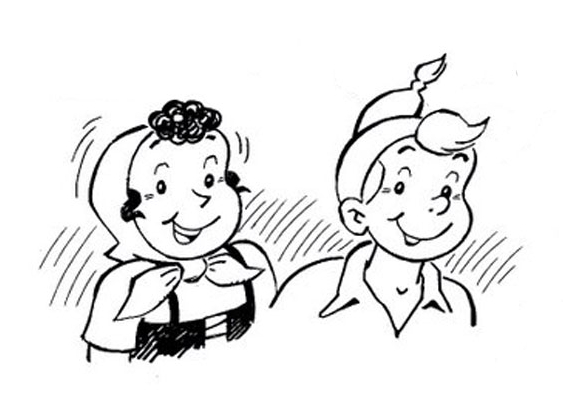
\includegraphics[width=.6\textwidth]{Sylvain+Sylvette_NB.jpg}} 
\newpage

\subsubsection{Exemple \no 7}

Sylvain part à bicyclette de A et se dirige vers B. Il roule à $20$ km/h.



Après avoir parcouru 8 km, il revient en A, s'arrête 12 minutes, puis repart vers B.

Sylvette va directement de A vers B. Elle roule à 16 km/h.

Sylvain et Sylvette sont partis en même temps de A et sont arrivés ensemble à B.

Quelle est la distance entre A et B ? 




\begin{enumerate}
\item \textbf{Choix de l'inconnue}

      Soit d la distance entre A et B. (l'unité est le kilomètre)

\item \textbf{ Mise en équation du problème}

Temps mis par Sylvain : $\dfrac{d+16}{20} + 0,2$

Temps mis par Sylvette : $\dfrac{d}{16}$

$\dfrac{d+16}{20} + \dfrac{1}{5} = \dfrac{d}{16} $


\item \textbf{ Résolution de l'équation}

$\dfrac{d+16}{20} + \dfrac{1}{5} = \dfrac{d}{16} $

$\dfrac{d+16}{20} + \dfrac{4}{20} = \dfrac{d}{16} $

$\dfrac{d+20}{20} = \dfrac{d}{16} $

$\dfrac{4\left(d+20\right)}{80} = \dfrac{5d}{80} $

$4\left(d+20\right) = 5d $

$ 4d + 80 = 5d$

$ -d = -80 $

$ d = 80 $

\item \textbf{ Réponse au problème}

La distance entre A et B est de 80 km.

\end{enumerate}


\newpage

\subsubsection{Exemple \no 8}



Sylvain et Sylvette partent simultanément pour effectuer un trajet de 54 km.


La vitesse de Sylvain est supérieure de 6 km/h à celle de Sylvette.

Sylvain arrive 45 min avant Sylvette.

Quelles sont les vitesses respectives de Sylvain et Sylvette ?



\begin{enumerate}
\item \textbf{Choix de l'inconnue}

Soit V la vitesse de Sylvette en km/h.

\item \textbf{Mise en équation du problème}

Temps mis par Sylvain : $\dfrac{54}{V+6}$

Temps mis par Sylvette : $\dfrac{54}{V}$

$\dfrac{54}{V+6} + \dfrac{3}{4} = \dfrac{54}{V}$

\item \textbf{Résolution de l'équation}

$\dfrac{54}{V+6} + \dfrac{3}{4} = \dfrac{54}{V}$

$\dfrac{216}{4V+24} + \dfrac{3V+18}{4V+24} = \dfrac{54}{V}$

$V\left(216+3V+18\right)=54\left(4V+24\right) $

$ 216V + 3V^2 + 18V = 216V + 1296 $

$ 3V^2 + 18V -1296 = 0 $

$ 3\left(V^2 + 6V - 432\right)=0 $

$ 3\left[\left(V^2 + 6V +9\right) - 441\right] = 0 $

$ 3\left(V+3\right)^2 - 21^2 = 0 $

$ 3\left(V + 3 + 21 \right)\left(V+3-21\right)=0 $

$ 3\left(V+24\right)\left(V-18\right) = 0 $ \\

\begin{tabular}{lcl}
$V+24 = 0$ & ou &$V-18=0$\\
$V=-24$ & ou &$V=18$\\
\end{tabular} \\

Une vitesse ne peut être négative, donc $V=18$.

On sait que la vitesse de Sylvain est $V+6$. Donc la vitesse de Sylvette est de 18 hm/h et celle de Sylvain 24 km/h.
\end{enumerate}



\ifdefined\COMPLETE
\else
    \end{document}
\fi             \newpage  $\;$ \newpage

\section{Inéquations à une inconnue}


\subsection{Inéquations du premier degré}

$ 2x - 5 \leqslant 0 $\\

$2x \leqslant 5 $\\

$ x \leqslant \dfrac{5}{2} $\\ 

Résoudre l'inéquation $ 2x-5\leqslant 0 $, c'est trouver l'ensemble des nombres réels x tels que :\\

$ 2x -5 \leqslant 0 $.

\vspace*{-.3cm}
\begin{tikzpicture}
     \tkzInit[xmin=-30,xmax=20,xstep=6]
     \tkzDrawX[label={},noticks,nograd]
     
     \tkzXHW    % I=]-10,7[
     {
%      -30/T//-10/T/],        % On hachure  de -inf à -10
        7/T/[/20/T/          % et de 9 à +inf
     }
%     \tkzText(-10,-.5){a}    % Etiquette gauche
     \tkzText(6.5,.6){$\dfrac{5}{2}$}      % Etiquette droite
%     \tkzText(0,0){\textcolor{red}{$\times$}}  % Etiquette croix sur R
%     \tkzText(0,-.3){\textcolor{red}{$x$}}     % Etiquette x sous croix
\end{tikzpicture}

$ S = \left]-\infty ; \dfrac{5}{2}\right[ $ \\

Néanmoins, il faut faire attention, car parfois, le sens se modifie : \\

$ -3x + 7 < 0 $\\

$ -3x < -7 $\\

$ 3x > 7 $\\

$ x > \dfrac{7}{3} $ 

\vspace*{-.3cm}
\begin{tikzpicture}
     \tkzInit[xmin=-30,xmax=20,xstep=6]
     \tkzDrawX[label={},noticks,nograd]
     
     \tkzXHW {
      -30/T//-10/T/]        % On hachure  de -inf à -10
%        7/T/[/20/T/          % et de 9 à +inf
     }
     \tkzText(-9.5,.6){$\dfrac{7}{3}$}    % Etiquette gauche
%     \tkzText(6.5,.6){$\dfrac{5}{2}$}      % Etiquette droite
%     \tkzText(0,0){\textcolor{red}{$\times$}}  % Etiquette croix sur R
%     \tkzText(0,-.3){\textcolor{red}{$x$}}     % Etiquette x sous croix
\end{tikzpicture}

\hspace*{4cm}$ S = \left]\dfrac{7}{3}, +\infty\right[ $ \\

\textbf{Attention à certaines inéquations}

$ 2x + 3 \leqslant x + 1 + x + 7 $\\

$ 2x - 2x \leqslant 1 + 7 - 3 $\\

$ 0x \leqslant 5 $ \\

Toujours vrai, donc : $ S = \R = \left]-\infty, +\infty\right[ $ \\

\newpage 

\textbf{Remarque}

Pour les 3 autres équations de la même famille, on aurait : 

$ 0x < 5 $ donne $ S = \R = \left]-\infty, +\infty\right[ $\\

$ 0x > 5 $ donne $ S = \varnothing $\\

$ 0x \geqslant 5 $ donne $ S = \varnothing $ \\

Pour $ 3 + 5x > 2 + 3x + 1 + 2x $, on a :\\

$ -3x - 2x + 5x > 1 + 2 - 3 $\\

$ 0x > 0 $ 

Impossible, donc $ S = \varnothing $ \\

\newpage 
\subsection{Signe de $\mathbf{ax+b}$ (Tableau de signes)}

\begin{tabular}{rl}
Soit : & $ f : \R \rightarrow \R$\\
& $ x\mapsto f(x) = ax + b $ avec $ a \neq 0 $ \\
&\\
& \textbf{Remarque}\\
& La fonction $f$ est une fonction affine, car $ f(x) = ax + b $\\
\end{tabular}

\subsubsection{Exemple \no 1}

Si $ f(x) = 2x-5 $ avec $a = 2$ et $b = -5$, on a : \\

\begin{tabular}{ccc}

$f(x) = 0$ & $f(x) < 0 $ & $f(x) > 0$ \\
\\
$2x - 5 = 0$ & $2x - 5 < 0$ & $2x - 5 > 0$ \\
$2x = 5 $ & $ 2x < 5 $ & $2x > 5 $ \\
$ x = \dfrac{5}{2} $ & $x <\dfrac{5}{2}$ & $x>\dfrac{5}{2}$ \\
\end{tabular}\\


\begin{tikzpicture} 

\tkzTabInit[lgt=2,espcl=1] 
{ $x$         /1, 
$2x-5$   /1}
{$ - \infty $ , $ \dfrac{5}{2} $ , $ + \infty $}
\tkzTabLine{ , - , z , + , }

\end{tikzpicture} 


\subsubsection{Exemple \no 2}

$ f(x) = -3x + 7 $ \\

\begin{tabular}{ccc}

$f(x) = 0$ & $f(x) < 0 $ & $f(x) > 0$ \\

$-3x +7 = 0$ & $-3x +7 < 0$ & $-3x +7 > 0$ \\
$-3x = -7 $ & $ -3x < -7 $ & $-3x > -7 $ \\
$ x = \dfrac{7}{3} $ & $x >\dfrac{7}{3}$ & $x<\dfrac{7}{3}$ \\
\end{tabular}

\begin{tikzpicture} 

\tkzTabInit[lgt=2,espcl=1] 
{ $x$         /1, 
$-3x+7$   /1}
{$ - \infty $ , $ \dfrac{7}{3} $ , $ + \infty $}
\tkzTabLine{ , + , z , - , }

\end{tikzpicture} 

\subsubsection{Tableau récapitulatif}

$ f(x) = ax + b $ avec $ a \neq 0 $ 

$ ax + b = 0 $

$ax = -b $

$ x = -\dfrac{b}{a} $

\vspace {.5cm}

\begin{tikzpicture} 

\tkzTabInit[lgt=4,espcl=3] 
{ $x$ /1, 
$ax+b$  /1}
{$ - \infty $ , $-\dfrac{b}{a} $ , $ + \infty $}
\tkzTabLine{ , $Signe de $-a$$ , z , $Signe de $a$$ }
\end{tikzpicture} 


\subsection{Inéquations produit}

\subsubsection*{Comment faire ?}

\textbf{Exemple \no 0}

$ \left(2x + 5\right)\left(-3x + 7\right) \leqslant 0 $ \\

Il faut faire un tableau de signes : \\

\begin{tikzpicture}

\tkzTabInit[lgt=3,espcl=2]
{ $x$  /1,
$2x+5$   /1,
$-3x + 7$ /1,
$\left(2x+5\right)\left(-3x+7\right)$ /1}
{$ - \infty $ , $-\dfrac{5}{2} $ , $\dfrac{7}{3} $ , $ + \infty $}
\tkzTabLine{ , - , z , +, t  ,+  }
\tkzTabLine{ , + , t , + , z, - }
\tkzTabLine{ , - , z , +, z, - }
\draw[decoration={brace, mirror, raise=0.2cm}, decorate, line width=2pt,black] (T14) -- (N24) ;
\draw[decoration={brace, mirror, raise=0.2cm}, decorate, line width=2pt,black] (N34) -- (T24) ;
\end{tikzpicture}
\\

\begin{tabular}{ccc}
$2x-5=0$& et &$-3x + 7 = 0$ \\
\\
$2x = -5$& et &$-3x = 7 $ \\
\\
$x= -\dfrac{5}{2}$& et & $x=\dfrac{7}{3}$ \\
\end{tabular}\\

\vspace{.1cm}

$ S = \left]-\infty, -\dfrac{5}{2}\right]\cup\left[\dfrac{7}{3},+\infty\right[ $ \\

\textbf{Exemple \no 1}\\

$ x^2 - 9 \leqslant 0 $\\

$ \left(x+3\right)\left(x-3\right) \leqslant 0 $\\

\begin{tabular}{lcl}

$x+3$ & ou & $ x - 3 = 0 $ \\
$x=-3$ & ou & $ x = 3 $ \\
\end{tabular}

\vspace{.5cm}

\begin{tikzpicture}
\tkzTabInit[lgt=3,espcl=2] 
{ $x$        /1 , 
$x+3$ /1 ,
$x-3$ /1,
$\left(x+3\right)\left(x-3\right)$ /1}
{$ -\infty $ , $-3 $ , $3$ , $ +\infty $}
\tkzTabLine{ , - , z , +, t  ,+  }
\tkzTabLine{ , - , t , - , z, + }
\tkzTabLine{ , + , z , -, z, + }
\end{tikzpicture} 

\newpage

\textbf{Exemple \no 2}

$ -x^2+5x < 0 $\\

$ x\left(-x+5\right) = 0$\\

\vspace{.5cm}

\begin{tikzpicture}
\tkzTabInit[lgt=3,espcl=2] 
{ $x$        /1 , 
$x$        /1 , 
$-x+5$ /1 ,
$x\left(-x+5\right)$ /1}
{$ -\infty $ , $0 $ , $5$ , $ +\infty $}
\tkzTabLine{ , - , z , +, t  ,+  }
\tkzTabLine{ , + , t , + , z, - }
\tkzTabLine{ , - , z , +, z, - }
\draw[decoration={brace, mirror, raise=0.2cm}, decorate, line width=2pt,black] (T14) -- (N24) ;
\draw[decoration={brace, mirror, raise=0.2cm}, decorate, line width=2pt,black] (N34) -- (T24) ;
\end{tikzpicture}
\\


$ S = \left]-\infty, 0 \right[\cup\left]5, +\infty\right[ $ \\

\textbf{Exercice \no 1}\\

$ x^2+24x-52 \geqslant 0 $

... 

$ \left(x+26\right)\left(x-2\right) \geqslant 0 $ \\

\begin{tabular}{ccc}
$x+26$ & ou & $x-2 = 0$ \\
$x=-26$ & ou &$x=2$ \\
\end{tabular}

\vspace{.5cm}

\begin{tikzpicture}

\tkzTabInit[lgt=3,espcl=2]
{ $x$  /1,
$x+26$   /1,
$x-2$ /1,
$\left(x+26\right)\left(x-2\right)$ /1}
{$ - \infty $ , $-26 $ , $2 $ , $ + \infty $}
\tkzTabLine{ , - , z , +, t  ,+  }
\tkzTabLine{ , - , t , - , z, + }
\tkzTabLine{ , + , z , -, z, + }
\draw[decoration={brace, mirror, raise=0.2cm}, decorate, line width=2pt,black] (T14) -- (N24) ;
\draw[decoration={brace, mirror, raise=0.2cm}, decorate, line width=2pt,black] (N34) -- (T24) ;
\end{tikzpicture}
\\

$ S = \left]-\infty, -26\right]\cup\left[2, +\infty\right[ $ \\


\newpage 

\textbf{Exercice \no 2}\\

$-9x^2+21x+8 > 0 $

...

$ \left(3x+1\right)\left(3x-8\right)<0 $

\begin{tabular}{ccc}
$3x + 1 = 0$ & ou & $3x - 8 = 0 $ \\
$x = -\dfrac{1}{3} $ & ou & $x=\dfrac{8}{3} $ \\
\end{tabular}\\

\begin{tikzpicture}
\tkzTabInit[lgt=3,espcl=2,]
{ $x$  /1,
$3x+1$   /1,
$3x - 8$ /1,
$\left(3x+1\right)\left(3x-8\right)$ /1}
{$ - \infty $ , $-\dfrac{1}{3} $ , $\dfrac{8}{3} $ , $ + \infty $}
\tkzTabLine{ , - , z , +, t  ,+  }
\tkzTabLine{ , - , t , - , z, + }
\tkzTabLine{ , + , z , -, z, + }
\draw[decoration={brace, mirror, raise=0.2cm}, decorate, line width=2pt,black] (N24) -- (N34) ;

\end{tikzpicture}

$ S = \left]-\dfrac{1}{3}, \dfrac{8}{3} \right[ $ \\

\textbf{Attentions à certaines inéquations}

\textbf{Exemple \no 1}\\

$ 49x^2 - 14x + 1 \leqslant 0 $\\

$ \left(7x-1\right)^2 \leqslant 0 $ \\

$ 7x - 1 = 0 $\\

$ 7x = 1 $\\

$ x = \dfrac{1}{7} $

\begin{tikzpicture}

\tkzTabInit[lgt=3,espcl=2]
{ $x$  /1,
$7x-1$   /1,
$7x-1$ /1,
$\left(7x-1\right)^2$ /1}
{$ - \infty $ , $\dfrac{1}{7} $ , $ + \infty $}
\tkzTabLine{ , - , z , +  }
\tkzTabLine{ , - , z , + }
\tkzTabLine{ , + , z , +, }
\end{tikzpicture}

$ S = \lb \dfrac{1}{7} \rb $ \\

\textbf{Remarque :}

Pour les 3 autres inéquations de la même famille, on aura :

\begin{tabular}{cc}
$49x^2 - 14x + 1 < 0$ & $S = \varnothing$ \\
$49x^2 - 14x + 1 \geqslant 0$& $ S = \R = \left]-\infty ; +\infty\right[$ \\
$49x^2 - 14x + 1 > 0$ & $ S = \left]-\infty ; \dfrac{1}{7} \right[\cup \left]\dfrac{1}{7}; +\infty\right[ $ \\
\end{tabular}

\newpage 

\textbf{Exemple \no 2} 

$ 25x^2 + 20x + 13 \leqslant 0 $\\

$ 25x^2 + 20x + 4 + 9 \leqslant 0 $\\

$ \left(5x + 2\right)^2 + 9 \leqslant 0 $\\

$ \left(5x + 2\right)^2 \leqslant - 9 $\\

Or, le carré d'un nombre est toujours positif. \\
Donc $ S = \varnothing $.\\

\textbf{Remarque :}

Pour les 3 autres inéquations de la même famille, on aura :

\begin{tabular}{cc}
$25x^2 + 20x + 13 < 0$ & $S = \varnothing$ \\
$25x^2 + 20x + 13 < 0$ & $ S = \R = \left]-\infty ; +\infty\right[$ \\
$25x^2 + 20x + 13 < 0$ & $ S = \R = \left]-\infty ; +\infty\right[$ \\
\end{tabular}

\newpage 
\subsection{Inéquation avec l'inconnue au dénominateur}

$ \dfrac{6}{x-2} \leqslant x-3 $\\

\textbf{Il ne faut pas que $ x-2 = 0 $ donc que $ x = 2 $}\\

\textbf{Valeur interdite : $ x = 2 $}\\

\textbf{Attention, dans le cas des inéquations, le produit en croix est interdit}\\

$ \dfrac{6}{x-2} - \left(x-3\right) \leqslant 0 $\\

$ \dfrac{6 - \left(x-2\right)\left(x-3\right)}{x-2} \leqslant 0 $\\

$ \dfrac{6 - \left(x^2 - 5x + 6 \right)}{x-2} \leqslant 0 $\\

$ \dfrac{-x^2 + 5x}{x-2} \leqslant 0 $\\

\vspace{.5cm}

\begin{tikzpicture}

\tkzTabInit[lgt=3,espcl=2,]
{ $x$  /1,
$x$ /1,
$-x+5$   /1,
$x -2 $ /1,
$\dfrac{x\left(-x+5\right)}{x-2}$ /1}
{$ - \infty $ , $0 $ , $2 $ , $5$ , $ + \infty $}
\tkzTabLine{ , - , z , +, t  ,+ , t , + }
\tkzTabLine{ , + , t , + , t , + , z, - }
\tkzTabLine{ , - , t , - , z , + , t , + }
\tkzTabLine{ , + , z , - , d , + , z , - }
\draw[decoration={brace, mirror, raise=0.2cm}, decorate, line width=2pt,black] (N25) -- (N35) ;
\draw[decoration={brace, mirror, raise=0.2cm}, decorate, line width=2pt,black] (N45) -- (T25) ;
\end{tikzpicture}
\\

$ S = \left[0,2\right[\cup \left[5, + \infty \right[ $ \\
\newpage
\textbf{Exercice \no 2} \\

$ \dfrac{x^2-15}{\left(x-4\right)\left(x-3\right)} \geqslant \dfrac{1}{x-4} - \dfrac{1}{x-3} $ \\

\textbf{Valeurs interdites : $x=4 $ et $ x = 3 $}  \\

$ \dfrac{x^2-15}{\left(x-4\right)\left(x-3\right)} \geqslant \dfrac{\left(x-3\right)-\left(x-4\right)}{\left(x-4\right)\left(x+3\right)} $ \\

$ \dfrac{x^2-15}{\left(x-4\right)\left(x-3\right)} \geqslant \dfrac{1}{\left(x-4\right)\left(x+3\right)} $ \\

$ \dfrac{x^2-15-1}{\left(x-4\right)\left(x-3\right)} \geqslant 0  $ \\

$ \dfrac{x^2-16}{\left(x-4\right)\left(x-3\right)} \geqslant 0  $ \\

$ \dfrac{\left(x+4\right)\left(x-4\right)}{\left(x-4\right)\left(x-3\right)} \geqslant 0  $ \\

\textbf{Remarque}

Simplifier est alors dangereux... Il est plus prudent d'écrire le tableau de signes ainsi : \\

\begin{tikzpicture}

\tkzTabInit[lgt=3,espcl=2]
{ $x$  /1,
$x+4$ /1,
$x-4$   /1,
$x-4 $ /1,
$x-3$ /1,
$\dfrac{x\left(x+4\right)\left(x-4\right)}{\left(x-4\right)\left(x-3\right)}$ /1}
{$ - \infty $ , $-4 $ , $3 $ , $4$ , $ + \infty $}
\tkzTabLine{ , - , z , +, t  ,+ , t , + }
\tkzTabLine{ , - , t , - , t , - , z, + }
\tkzTabLine{ , - , t , - , t , - , z, + }
\tkzTabLine{ , - , t , - , z , + , t , + }
\tkzTabLine{ , + , z , - , d , + , d , + }
\draw[decoration={brace, mirror, raise=0.2cm}, decorate, line width=2pt,black] (T16) -- (N26) ;
\draw[decoration={brace, mirror, raise=0.2cm}, decorate, line width=2pt,black] (N36) -- (N46) ;
\draw[decoration={brace, mirror, raise=0.2cm}, decorate, line width=2pt,black] (N46) -- (T26) ;
\end{tikzpicture}\\

$S=\left]-\infty,-4\right]\cup\left]3,4\right[\cup\left]4,+\infty\right[$

\newpage 
\subsection{Systèmes d'inéquations}

\subsubsection{Exemple \no 1}

\vspace*{.5cm}

\begin{minipage}{3cm}
\begin{equation*}
\left\lbrace \begin{aligned}
2x+3      &> 3x-2\\
3(x-2)    &\geqslant 2-5x\\
\end{aligned}
\right.
\end{equation*}
\end{minipage}

\vspace*{.5cm}

Résoudre un tel système, c'est trouver l'ensemble des nombres réels $x$ \\
tels que $ 2x + 3 > 3x - 2 $ 
\textbf{et} $ 3\left(x-2\right) \geqslant 2 -5x $\\

\textbf{1$^{re}$ inéquation :}\\

$2x + 3 > 3x - 2$\\

$- x > -5$\\

$x < 5$ \\

$ S_1 = \left]-\infty, 5 \right[ $ \\

\textbf{2$^{me}$ inéquation :}\\

$ 3\left(x-2\right) \geqslant 2 - 5x $\\

$ 3x - 5 \geqslant 2 - 5x $\\

$ 8 x \geqslant 8 $\\

$ x \geqslant 1 $ \\

$ S_2 = \left[1, +\infty\right[ $ \\

\textbf{3 : Système}\\

$ S = S_1 \cap S_2 $


\vspace*{-.3cm}
\begin{tikzpicture}
     \tkzInit[xmin=-30,xmax=20,xstep=6]
     \tkzDrawX[label={},noticks,nograd]
     
      \tkzDefPoint(-30,-.05){A1} 
      \tkzDefPoint(7,-.05){A2} 
     \tkzDrawSegment[color=green](A1,A2) ; 
       \tkzXHW [color=green]  % XHW : hachures SW -> NE  
     {
%      -30/T//-10/T/],        % On hachure  de -inf à -10
        7/T/[/20/T/          % et de 9 à +inf
     }
        
     \tkzDefPoint(-10,.05){B1} 
      \tkzDefPoint(20,.05){B2} 
     \tkzDrawSegment[color=red](B1,B2) ; 
     \tkzXH [color=red]   % XH : hachures NW -> SE
     {
      -30/T//-10/T/[        % On hachure  de -inf à -10
%        7/T/[/20/T/          % et de 9 à +inf
     }
     
     \tkzText(-10,.5){$1$}    % Etiquette gauche
     \tkzText(6.5,.6){$5$}      % Etiquette droite
%     \tkzText(0,0){\textcolor{red}{$\times$}}  % Etiquette croix sur R
%     \tkzText(0,-.3){\textcolor{red}{$x$}}     % Etiquette x sous croix
\end{tikzpicture}


$ S= \left[1,5\right[ $
\newpage
\subsubsection{Exemple \no 2}

\vspace*{.5cm}

\begin{minipage}{3cm}
\begin{equation*}
\left\lbrace \begin{aligned}
\dfrac{3}{5}x     &  >     \dfrac{1}{5} + x \\
6\left(2-x\right) & \leqslant   -2x \\
\end{aligned}
\right.
\end{equation*}
\end{minipage}

\vspace*{.5cm}

\textbf{1$^{re}$ inéquation :}

$ \dfrac{3}{5}x - x > \dfrac{1}{5} $\\

$ x \left(\dfrac{3}{5} - 1\right) > \dfrac{1}{5} $\\

$ -\dfrac{2}{5}x > \dfrac{1}{5} $\\

$ x < \dfrac{1}{5} \times \left(-\dfrac{5}{2}\right) $\\

$ x < -\dfrac{1}{2} $ \\

$ S_1 = \left]-\infty, -\dfrac{1}{2} \right[ $\\

\textbf{2$^{me}$ inéquation :}

$12 - 6x \leqslant -2x $\\

$ -4x \leqslant -12 $\\

$ 4x \geqslant 12 $\\

$ x \geqslant 3 $ \\

$ S_2 = \left[3, +\infty\right[ $\\

\textbf{3 : Système}\\

$ S = S_1 \cap S_2 = \varnothing $\\

\vspace*{-.3cm}
\begin{tikzpicture}   
     \tkzInit[xmin=-5,xmax=7]
     \tkzDrawX[label={},noticks,nograd]
     
      \tkzDefPoint(3,.1){A1} 
      \tkzDefPoint(7,.1){A2} 
     \tkzDrawSegment[color=red](A1,A2) ; 
       \tkzXH [color=red]  % XHW : hachures SW -> NE  
     {
        -5/T//3/T/[          % True de 3 à +inf 
     }
        
     \tkzDefPoint(-5,-.1){B1} 
      \tkzDefPoint(-1/2,-.1){B2} 
     \tkzDrawSegment[color=blue](B1,B2) ; 
     \tkzXHW [color=blue]   % XH : hachures NW -> SE
     {
      -.5/T/[/7/T/        % On hachure  de -inf à -10
     }
     
    \tkzText(-1/2,.5){$-\dfrac{1}{2}$}    % Etiquette gauche
    \tkzText(3,.6){$3$}      % Etiquette droite
\end{tikzpicture}

\textbf{Remarque}

Les 2 inéquations sont incompatibles.
\newpage 
\subsubsection{Exercice \no 1}

\begin{minipage}{3cm}
\begin{equation*}
\left\lbrace \begin{aligned}
4x^2 + 3x + 1&\geqslant x^2 - 3x + 1\\
\left(x+1\right)^2&> 5x+5 \\
\end{aligned}
\right.
\end{equation*}
\end{minipage}

\vspace{.5cm}

\textbf{1$^{re}$ inéquation}\\

$ 3x^2 + 6x \geqslant 0 $

$ 3x \left(x+2\right) \geqslant 0 $\\ 

\begin{tikzpicture}
\tkzTabInit[lgt=3,espcl=2]
{ $x$  /1,
$3x$ /1,
$x+2$   /1,
$3x\left(x+2\right)$ /1}
{$ - \infty $ , $-2 $ , $0 $ , $ + \infty $}
\tkzTabLine{ , - , t , -, z  ,+ }
\tkzTabLine{ , - , z , + , t , + }
\tkzTabLine{ , + , z , - , z , + }
\draw[decoration={brace, mirror, raise=0.2cm}, decorate, line width=2pt,black] (T14) -- (N24) ;
\draw[decoration={brace, mirror, raise=0.2cm}, decorate, line width=2pt,black] (N34) -- (T24) ;
\end{tikzpicture}


$ S_1 = \left]-\infty, -2\right]\cup[0,+\infty[ $ \\

\textbf{2$^{me}$ inéquation}\\

$ \left(x+1\right)^2 > 5\left(x+1\right) $

$ \left(x+1\right)^2 - 5\left(x+1\right)  > 0 $

$ \left(x+1\right)\left(x+1-5\right) > 0 $

$ \left(x+1\right)\left(x-4\right) > 0 $\\



\begin{tikzpicture}
\tkzTabInit[lgt=3,espcl=2]
{ $x$  /1,
$x+1$ /1,
$x-4$   /1,
$\left(x+1\right)\left(x-4\right)$ /1}
{$ - \infty $ , $-1 $ , $4 $ , $ + \infty $}
\tkzTabLine{ , - , z , +, t  ,+ }
\tkzTabLine{ , - , t , - , z , + }
\tkzTabLine{ , + , z , - , z , + }
\draw[decoration={brace, mirror, raise=0.2cm}, decorate, line width=2pt,black] (T14) -- (N24) ;
\draw[decoration={brace, mirror, raise=0.2cm}, decorate, line width=2pt,black] (N34) -- (T24) ;
\end{tikzpicture}\\

$ S_2 = \left]-\infty, -1\right[\cup\left]4, + \infty \right[ $\\

\textbf{3 : Système}

$ S = S_1 \cap S_2 = \left]-\infty, -2\right]\cup\left]4, + \infty\right[ $\\


\begin{tikzpicture}   
     \tkzInit[xmin=-5,xmax=7]
     \tkzDrawX[label={},noticks,nograd]
     
      \tkzDefPoint(-5,.1){A1} 
      \tkzDefPoint(-1,.1){A2} 
      \tkzDefPoint(4,.1){A3} 
      \tkzDefPoint(7,.1){A4} 
      \tkzDrawSegments[color=red](A1,A2 A3,A4) ; 
       \tkzXHW [color=red]   
     {
        -1/T/[/4/T/]          
     }
        
     \tkzDefPoint(-5,-.1){B1} 
     \tkzDefPoint(-2,-.1){B2}
     \tkzDefPoint(0,-.1){B3} 
     \tkzDefPoint(7,-.1){B4}  
     \tkzDrawSegments[color=blue](B1,B2 B3,B4) ; 
     \tkzXH [color=blue]  
     {
      -2/T/]/0/T/[       
     }
     
    \tkzText(-2,.5){$-2$} 
    \tkzText(-1,.5){$-1$}  
    \tkzText(0,.5){$0$}   
    \tkzText(4,.5){$4$}  
\end{tikzpicture}

\newpage 

\subsubsection{Exercice \no 2}

$ 0 \leqslant \left(3x-8\right)^2-\left(x-4\right)^2 \leqslant 48 $

C'est une \textbf{double inéquation}, cela veut dire que : \\

$ \left(3x-8\right)^2-\left(x-4\right)^2 \geqslant 0 $

$ \left(3x-8\right)^2-\left(x-4\right)^2 \leqslant 48 $ \\

\textbf{1$^{re}$ inéquation}

$ \left(3x-8+x+4\right)\left[\left(3x-8\right)-\left(x+4\right)\right] \geqslant 0 $

$ \left(3x-8+x+4\right)\left(3x-8-x-4\right) \geqslant 0 $

$ \left(4x-4\right)\left(2x-12\right) \geqslant 0 $ \\

\begin{tikzpicture}
\tkzTabInit[lgt=3,espcl=2]
{ $x$  /1,
$4x-4$ /1,
$2x-12$   /1,
$\left(4x-4\right)\left(2x-12\right)$ /1}
{$ - \infty $ , $1 $ , $6 $ , $ + \infty $}
\tkzTabLine{ , - , z , +, t  ,+ }
\tkzTabLine{ , - , t , - , z , + }
\tkzTabLine{ , + , z , - , z , + }
\draw[decoration={brace, mirror, raise=0.2cm}, decorate, line width=2pt,black] (T14) -- (N24) ;
\draw[decoration={brace, mirror, raise=0.2cm}, decorate, line width=2pt,black] (N34) -- (T24) ;
\end{tikzpicture}

$ S_1 = \left]-\infty, 1 \right]\cup\left[6, + \infty\right[ $ \\

\textbf{2$^{me}$ inéquation}

$ \left(3x-8\right)^2-\left(x+4\right)^2 \leqslant 48 $

$ \left(9x^2 - 48x + 64\right)-\left(x^2+8x+16\right) \leqslant 48 $

$ 9x^2 - 48x + 64 -x^2- 8x- 16 \leqslant 48 $

$ 8x^2 -56x + 48 \leqslant 48 $

$ 8x^2 - 56x \leqslant 0 $

$ 8x \left(x-7\right)\leqslant 0 $\\

\begin{tikzpicture}
\tkzTabInit[lgt=3,espcl=2]
{ $x$  /1,
$8x$ /1,
$x-7$   /1,
$8x\left(x-7\right)$ /1}
{$ - \infty $ , $0 $ , $7 $ , $ + \infty $}
\tkzTabLine{ , - , z , +, t  ,+ }
\tkzTabLine{ , - , t , - , z , + }
\tkzTabLine{ , + , z , - , z , + }
\draw[decoration={brace, mirror, raise=0.2cm}, decorate, line width=2pt,black] (N24) -- (N34) ;
\end{tikzpicture}

$ S_2 = \left[0,7\right] $ \\

\textbf{3 : Système}\\

$ S = S_1 \cap S_2 = \left[0,1\right]\cup \left[6,7\right] $\\

\begin{tikzpicture}   
     \tkzInit[xmin=-2,xmax=9]
     \tkzDrawX[label={},noticks,nograd]
 
       \tkzXHW [color=blue]   
     {
        -2/T//0/T/[,   
         7/T/]/9/T/           
     }

     \tkzXH [color=blue]  
     {
      1/T/]/6/T/[       
     }
     
    \tkzText(0,.5){$0$} 
    \tkzText(1,.5){$1$}  
    \tkzText(6,.5){$6$}   
    \tkzText(7,.5){$7$}  
\end{tikzpicture}
\subsubsection{Exercice \no 3}

$ 2 \leqslant \dfrac{x+5}{x+2} \leqslant 3 $ \\

\textbf{Valeur interdite : $\mathbf{x = -2 }$} \\

Pour la première inéquation, on a :\\

$ \dfrac{-x+1}{x+2} \geqslant 0 $ \\

\vspace{.5cm}

\begin{tikzpicture}
\tkzTabInit[lgt=3,espcl=2]
{ $x$  /1,
$-x+1$ /1,
$x+2$   /1,
$\left(-x+1\right)\left(x+2\right)$ /1}
{$ - \infty $ , $-2 $ , $1 $ , $ + \infty $}
\tkzTabLine{ , + , t , +, z  ,- }
\tkzTabLine{ , - , z , + , t , + }
\tkzTabLine{ , - , d , + , z , - }
\draw[decoration={brace, mirror, raise=0.2cm}, decorate, line width=2pt,black] (N24) -- (N34) ;
\end{tikzpicture}
\\

$ S_1 = \left]-2, 1 \right] $ \\

Pour la deuxième inéquation, on a : \\

$ \dfrac{-2x-1}{x+2} \leqslant 0 $ \\

\vspace{.5cm}

\begin{tikzpicture}
\tkzTabInit[lgt=3,espcl=2]
{ $x$  /1,
$-2x-1$ /1,
$x+2$   /1,
$\left(-2x-1\right)\left(x+2\right)$ /1}
{$ - \infty $ , $-2 $ , $-\dfrac{1}{2} $ , $ + \infty $}
\tkzTabLine{ , +, t , +, z  ,- }
\tkzTabLine{ , - , z , + , t , + }
\tkzTabLine{ , - , d , + , z , - }
\draw[decoration={brace, mirror, raise=0.2cm}, decorate, line width=2pt,black] (T14) -- (N24) ;
\draw[decoration={brace, mirror, raise=0.2cm}, decorate, line width=2pt,black] (N34) -- (T24) ;
\end{tikzpicture}
\\

$ S_2 = \left]-\infty,-2\right[\cup\left[-\dfrac{1}{2}, +\infty \right[ $ \\

$  S = S_1 \cap S_2 = \left[-\dfrac{1}{2}, 1 \right] $\\

\begin{tikzpicture}   
     \tkzInit[xmin=-4,xmax=3]
     \tkzDrawX[label={},noticks,nograd]
 
       \tkzXHW [color=blue]   
     {
        -4/T//-2/T/],   
         1/T/]/3/T/           
     }

     \tkzXH [color=blue]  
     {
      -2/T/]/-.5/T/[       
     }
     
    \tkzText(-2,.5){$-2$} 
    \tkzText(-1/2,.5){$-\dfrac{1}{2}$}  
    \tkzText(1,.5){$1$}   
\end{tikzpicture}

\newpage

\subsection{Exemples de problèmes pratiques}

\subsubsection{Exemple \no 1}

Un motard poursuit une voiture sur l'autoroute. La voiture est à $150$ km de la sortie. Elle roule à 120 km/h. \\ 

Le motard est à $x$ km derrière la voiture. Il roule à $130$ km/h. \\ 

Pour quelles valeurs de $x$ Sylvain rattrape-t-il Sylvette, avant la sortie de l'autoroute ? \\

\textbf{1) Choix de l'inconnue.}

Soit $x$ la distance, en km, qui sépare le motard de la voiture. \\

\textbf{2) Mise en équation du problème} \\

Temps mis par le motard  : $\dfrac{x+150}{130} $ \\

Temps mis par la voiture : $\dfrac{150}{120} $ \\

Donc $ \dfrac{x+150}{130} \leqslant \dfrac{150}{120}$ \\

\textbf{3) Résolution de l'équation}

$ \dfrac{x+150}{130} \leqslant \dfrac{150}{120}$ \\

$ \dfrac{x+150}{130} \leqslant \dfrac{5}{4}$ \\

$ \dfrac{2\left(x+150\right)}{260} \leqslant \dfrac{325}{260} $ \\

$ 2x + 300 \leqslant 325 $ \\

$ 2x \leqslant 25 $ \\

$ x \leqslant 12,5 $ \\

\textbf{4) Réponse au problème}

Donc le motard rattrapera la voiture si la distance qui le sépare est inférieur à $12,5$ km. \\

\newpage

\subsubsection{Exemple \no 2}

Voici les tarifs pratiqués par 3 agences de location de voiture pour des véhicules identiques : \\

\begin{itemize}
\item Agence A : $52,74$\euro par jour et $0,41$ \euro par km ; 
\item Agence B : $43,14$\euro  par jour et $0,49$ \euro par km ; 
\item Agence C : $47,40$\euro par jour et $0,44$ \euro par km. \\
\end{itemize} 

Sylvain et Sylvette désirent parcourir $x$ km par jour. Quelle agence choisissent-ils ? \\

\begin{enumerate}


\item \textbf{Choix de l'inconnue.}

Soit $x$ le nombre de km parcourus. \\

\item \textbf{ Mise en équation du problème} \\

$P_A(x) = 52,74$\euro $+0,41x$ 

$P_B(x) = 43,14$\euro $+0,49x$ 

$P_C(x) = 57,40$\euro $+0,44x$ \\

Sylvain et Sylvette choisissent l'agence A si $P_A(x) \leqslant P_B(x)$ et $ P_A(x) \leqslant P_C(x)$. 

Sylvain et Sylvette choisissent l'agence B si $P_B(x) \leqslant P_A(x)$ et $ P_B(x) \leqslant P_C(x)$. 

Sylvain et Sylvette choisissent l'agence C si $P_C(x) \leqslant P_A(x)$ et $ P_C(x) \leqslant P_B(x)$. \\

\item \textbf{Résolution de l'équation} \\

\begin{enumerate}


\item {$\begin{cases}
52,74+0,41x &\leqslant 43,14+0,49x\\
52,74+0,41x & \leqslant 57,40+0,44x\\
\end{cases}$}

\begin{enumerate}


\item $52,74+0,41x \leqslant 43,14+0,49x$ 

$ -0,08x \leqslant -9,6 $

$ 0,08 \geqslant 9,6 $

$ x \geqslant 120 $ \\

\item $52,74+0,41x \leqslant 57,40+0,44x$

$-0,03x \leqslant -5,34$ 

$ 0,03x \geqslant  5,34 $

$ x \geqslant 178 $ \\


\begin{tikzpicture}   
     \tkzInit[xmin=8,xmax=20]
     \tkzDrawX[label={},noticks,nograd]
 
       \tkzXH [color=blue]   
     {
        8/T//17.8/T/|            
     }

     \tkzXHW [color=blue]  
     {
      8/T//12/T/|       
     }
     
    \tkzText(12,1){$120$} 
    \tkzText(17.8,1){$178$}     
\end{tikzpicture}

Sylvain et Sylvette choisissent l'agence A s'ils parcourent une distance supérieure à $178$ km. \\
\end{enumerate}
\newpage

\item  $\begin{cases}
43,14+0,49x &\leqslant 52,74+0,41x\\
43,14+0,49x & \leqslant 57,40+0,44x\\
\end{cases}$  \\

\begin{enumerate}
\item $43,14+0,49x \leqslant 52,74+0,41x$ \\

       D'après (a)i. , on a : $x\leqslant 120$ \\

\item $43,14+0,49x \leqslant 57,40+0,44x$\\

$0,05x \leqslant 4,26 $\\

$x \leqslant 85,2 $ \\


\begin{tikzpicture}   
     \tkzInit[xmin=8,xmax=20]
     \tkzDrawX[label={},noticks,nograd]
 
       \tkzXH [color=blue]   
     {
        12/T/|/20/T/            
     }

     \tkzXHW [color=blue]  
     {
      8.52/T/|/20/T/       
     }

    \tkzText(8.52,1){$85,2$}       
    \tkzText(12,1){$120$} 
   
\end{tikzpicture}


Sylvain et Sylvette choisissent l'agence $B$ s'ils parcourent une distance inférieure à $85,2$ km. 
\end{enumerate}

\item  $\begin{cases}
57,40+0,44x &\leqslant 52,74+0,41x\\
57,40+0,44x & \leqslant 43,14+0,49x\\
\end{cases}$  \\

\begin{enumerate}


\item  D'après (a)ii, on a : $x 178$ \\

\item 
 D'après (b)ii, on a : $x\geq 85,2$ \\

\end{enumerate}
\end{enumerate}
\end{enumerate}

\begin{tikzpicture}   
     \tkzInit[xmin=5,xmax=20]
     \tkzDrawX[label={},noticks,nograd]
 
       \tkzXHW [color=blue]   
     {
        17.8/T/|/20/T/            
     }

     \tkzXH [color=blue]  
     {
      5/T//8.52/T/|       
     }

    \tkzText(8.52,1){$85,2$}       
    \tkzText(17.8,1){$178$} 
   
\end{tikzpicture}

Sylvain et Sylvette choisissent l'agence $C$ s'ils parcourent une distance comprise entre $85,2$ km et $178$ km. \\


           \newpage  $\;$ \newpage
\ifdefined\COMPLETE
\else
    \input{./preambule-sacha-utf8.ltx}
    \begin{document}
\fi

\section{Fonctions numérique de la variable réelle : Généralités et définitions}

\subsection{Fonction}

\begin{tabular}{lll}
Soit & $f:$ & $ \R \rightarrow \R$ \\
& & $x\mapsto \underbrace{f(x)}_{\textrm{image de} x}$ \\
\end{tabular}

$f$ est une fonction numérique de la variable réelle si et seulement si :

\textbf{Tout élément de $\mathbf{\R}$ a au plus une image dans $\mathbf{\R}$.} \\

\textbf{Remarques}

\begin{itemize}


\item[*]Vocabulaire : "Au plus une" veut dire, soit une, soit aucune. \\ 

\item[*] $f$ est une fonction et $f(x)$ un nombre réel.
\end{itemize}
\subsection{Ensemble de définition d'une fonction}

\begin{tabular}{lll}

Soit & $f:$& $ \R \rightarrow \R$ \\
& & $x\mapsto f(x)$ \\
\end{tabular}

\textbf{L'ensemble de définition de f, noté $ \mathbf{D_f} $, est l'ensemble de élément de $\mathbf{\R}$\\qui ont une image dans $\mathbf{\R}$}


\begin{minipage}{5cm}
\begin{tikzpicture}[scale=.8]

\tkzDefPoint [label=left:$a$](0,1.5){a}
\tkzDrawPoint[size=10,color=black](a)
\tkzDefPoint [label=left:$b$](0,1){b}
\tkzDrawPoint[size=10,color=black](b)
\tkzDefPoint [label=left:$c$](0,.5){c}
\tkzDrawPoint[size=10,color=black](c)
\tkzDefPoint [label=left:$d$](0,0){d}
\tkzDrawPoint[size=10,color=black](d)
\tkzDefPoint [label=right:$\Delta$](3,1.5){de}
\tkzDrawPoint[size=10,color=black](de)
\tkzDefPoint [label=right:$\bigstar$](3,1){st}
\tkzDrawPoint[size=10,color=black](st)
\tkzDefPoint [label=right:$\bigcirc$](3,.5){nada}
\tkzDrawPoint[size=10,color=black](nada)



\node [draw,ellipse,minimum height=3cm,minimum width=1.5cm, fit={(a) (b) (c) (d) }] {};
\node [draw,ellipse,minimum height=3cm,minimum width=1cm,fit={(de) (st) (nada) }] {};

\draw  [bend left=20,-latex](a) to (de) ; 
\draw  [bend right=20,-latex](b) to (de) ; 
\draw  [bend right=20,-latex](c) to (st) ; 
\end{tikzpicture}
\end{minipage}
\begin{minipage}{3cm}

$f(a) = \Delta$

$f(b) = \Delta$

$f(c) = \bigstar $ \\

$ D_f = \lb a, b, c \rb $

$D_f = E \setminus\lb d \rb $

\end{minipage}\\


\subsubsection{Exercice \no 1}

\begin{tabular}{llll}
Soit & $f:$& $ \R \rightarrow \R$ & \\
& & $x\mapsto f(x)$ & $=\dfrac{x-4}{x-2}$ \\
\end{tabular}\\

Il ne faut pas que $x-2=0$, donc que $x=2$.

$D_f = \R \setminus \lb 2 \rb = \left]-\infty,2\right[\cup\left]2, +\infty\right[$

\subsubsection{Exercice \no 2}

\begin{tabular}{llll}

Soit & $f:$& $ \R \rightarrow \R$ & \\
& & $x\mapsto f(x)$ & $=\sqrt{x-2}$ \\
\end{tabular}\\

Il faut que $x-2 \geqslant 0$, donc que $x \geqslant 2 $

$D_f = \left[2, +\infty\right[ $

\newpage

\subsubsection{Exercice \no 3}

\begin{tabular}{llll}

Soit & $f:$& $ \R \rightarrow \R$ & \\
& & $x\mapsto f(x)$ & $=\dfrac{x^2 + 4}{x^2 - 4}$ \\
\end{tabular}\\

Il ne faut pas que $x^2 - 4 = 0$, donc que $\left(x+2\right)\left(x-2\right) = 0 $

\begin{tabular}{lll}
$x+2=0$ & ou & $x-2 = 0 $ \\
$x = -2 $ & ou & $x=2$ \\
\end{tabular}

$ D_f = \R \setminus\lb -2,2\rb = \left]-\infty, -2\right[\cup \left]-2,2\right[\cup\left]2, +\infty\right[ $

\subsubsection{Exercice \no 4}

\begin{tabular}{llll}

Soit & $f:$& $ \R \rightarrow \R$ & \\
& & $x\mapsto f(x)$ & $=\sqrt{x^2 - 4}$ \\
\end{tabular}

Il faut que $x^2 - 4 \geqslant 0 $, donc que $\left(x+2\right)\left(x-2\right) \geqslant 0$

\begin{tikzpicture}
\tkzTabInit[lgt=3,espcl=2]
{ $x$  /1,
$x+2$ /1,
$x-2$   /1,
$\left(x+2\right)\left(x-2\right)$ /1}
{$ - \infty $ , $-2 $ , $2 $ , $ + \infty $}
\tkzTabLine{ , - , z , +, t  ,+ }
\tkzTabLine{ , - , t , - , z , + }
\tkzTabLine{ , + , z , - , z , + }
\draw[decoration={brace, mirror, raise=0.2cm}, decorate, line width=2pt,black] (T14) -- (N24) ;
\draw[decoration={brace, mirror, raise=0.2cm}, decorate, line width=2pt,black] (N34) -- (T24) ;
\end{tikzpicture}

$D_f = \left]-\infty,-2\right[\cup\left[2,+\infty\right[ $

\subsubsection{Exercice \no 5}

\begin{tabular}{llll}

Soit & $f:$& $ \R \rightarrow \R$ & \\
& & $x\mapsto f(x)$ & $=\dfrac{x^2 - 4}{x^2 + 4}$ \\
\end{tabular}\\

Il ne faut pas que $x^2 + 4 = 0$, donc $x^2 = -4$.

Ceci est impossible, donc $D_f = \R$.

\textbf{Remarque}

Il s'agit du problème de la continuité.

\subsubsection{Exercice \no 6}

\begin{tabular}{llll}

Soit & $f:$& $ \R \rightarrow \R$ & \\
& & $x\mapsto f(x)$ & $=\sqrt{x^2 + 4}$ \\
\end{tabular}

Il faut que $x^2+4 \geqslant 0$, donc $x^2 \geqslant -4$

Ceci est toujours vrai, donc $D_f = \R$.

\subsection{Représentation graphique d'une fonction}

\begin{tabular}{lll}

Soit & $f:$& $ \R \rightarrow \R$ \\
& & $x\mapsto f(x)$ \\
\end{tabular}\\

Soit $\left(0, \overrightarrow{i}, \overrightarrow{j}\right)$ un repère.

La représentation graphique de $f$, notée $C_f$, est l'ensemble des points $M\left(x,y\right)$ avec $x\in D_f$ et $y = f(x)$.

\newpage

\vspace*{-2cm}
\textbf{I}\\

\centerline{
\begin{minipage}{.45\textwidth}
\shorthandoff{:}
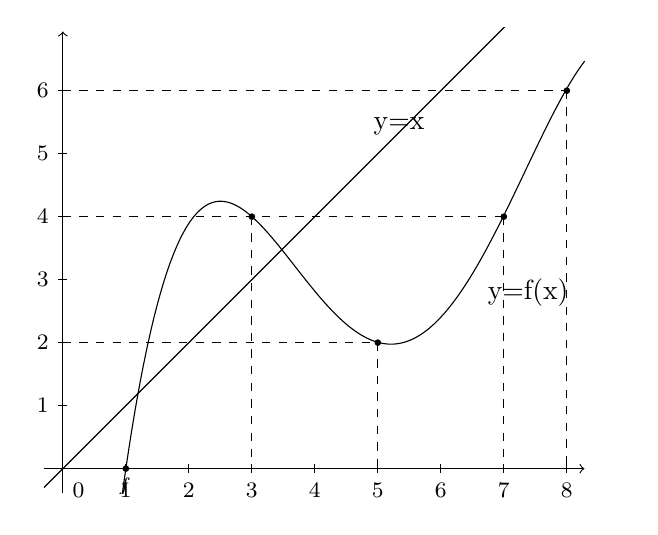
\begin{tikzpicture}[scale=0.8]
\draw[->,color=black] (-0.3,0) -- (8.28,0);
\foreach \x in {,1,2,3,4,5,6,7,8}
\draw[shift={(\x,0)},color=black] (0pt,2pt) -- (0pt,-2pt) node[below] {\footnotesize $\x$};
\draw[->,color=black] (0,-0.38) -- (0,6.94);
\foreach \y in {,1,2,3,4,5,6}
\draw[shift={(0,\y)},color=black] (2pt,0pt) -- (-2pt,0pt) node[left] {\footnotesize $\y$};
\draw[color=black] (0pt,-10pt) node[right] {\footnotesize $0$};
\clip(-0.3,-0.4) rectangle (9,7);
\draw[smooth,samples=100,domain=-0.301:8.284] plot(\x,{
-(29/840)*(\x)^4 
+(213/280)*(\x)^3 
-(4699/840)*(\x)^2 
+(4443/280)*\x 
-11});
\draw [dashed] (3,4)-- (3,0);
\draw [dashed] (0,4)-- (7,4);
\draw [dashed] (7,4)-- (7,0);
\draw [dashed] (0,2)-- (5,2);
\draw [dashed] (5,2)-- (5,0);
\draw [dashed] (0,6)-- (8,6);
\draw [dashed] (8,6)-- (8,0);
\draw[smooth,samples=100,domain=-0.301:8.284] plot(\x,{(\x)});
\draw (6.59,3.17) node[anchor=north west] {y=f(x)};
\draw (4.78,5.72) node[anchor=north west] {y=x};
\begin{scriptsize}
\fill (1,0) circle (1.5pt);
\fill (3,4) circle (1.5pt);
\fill (5,2) circle (1.5pt);
\fill (7,4) circle (1.5pt);
\draw(0.98,-0.29) node {$f$};
\fill (8,6) circle (1.5pt);
\end{scriptsize}
\end{tikzpicture}
\shorthandon{:}
\end{minipage} \hspace*{1cm}
\begin{minipage}{.45\textwidth}
On a représenté ci-contre : \\
\begin{itemize}
\item[*] La droite d'équation $y=x$ ; 
\item[*] La courbe représentative d'une fonction $f$ définie sur l'intervalle $[1;8]$. 
\end{itemize}
Les question posées seront résolues par {\bf lecture graphique}. 
\end{minipage}}
\vspace{.5cm}
Répondre par vrai ou faux aux questions suivantes : 

\vspace{.1cm}

\begin{tabular}{|l|c|l}
\multicolumn{2}{r}{vrai ou faux} & \\
\cline{1-2}
$1$ a pour image $0$ par la fonction $f$ & \textcolor{blue} {\it \Large V } & \\
\cline{1-2}
$0$ a pour image $1$ par la fonction $f$ & \textcolor{blue} {\it \Large F } & \\
\cline{1-2}
$5$ est un antécédent de $2$ par la fonction $f$ & \textcolor{blue} {\it \Large V } & \\
\cline{1-2}
$4$ a deux  antécédents  par la fonction $f$ : $3$ et $7$ &  \textcolor{blue} {\it \Large F}& \\
\cline{1-2}
\textcolor{blue} {\it Combien 3 a-t-il d'antécédents ? }& \textcolor{blue} {\it \Large 3 }&\\
\cline{1-2}
& \\
\cline{1-2}
$f(3) \leqslant f(5) $ & \textcolor{blue} {\it \Large F } &\\
\cline{1-2}
$f$ est croissante sur l'intervalle $[1 ; 8]$ & \textcolor{blue} {\it \Large V } & pas strictement\\
\cline{1-2}
& \\
\cline{1-2}
& \\
\cline{1-2}
L'équation $f(x) = x $ a au moins une solution dans l'intervalle $[1 ; 8]$ &  \textcolor{blue} {\it \Large V } &\\
\cline{1-2}
Si $x$ appartient à l'intervalle $[3 ; 5]$ alors $f(x) \leqslant x $ & \textcolor{blue} {\it \Large F } &\\
\cline{1-2}
\end{tabular}

\medskip 

\textbf{II}\\

On considère la fonction $f$ définie sur l'intervalle $[-7 ; 4]$ par sa représentation graphique $\mathcal{C}$ et la fonction $g$ dont la représentation graphique est la droite $d$.
 
\centerline{
\begin{minipage}{.6\textwidth}
\textbf{Répondre aux questions suivantes par lecture graphique}
\begin{enumerate}
\item  \begin{enumerate}
        \item Quelles sont les images par $f$ des réels $-3$ et $0$ ? 
        \item  Quels sont les antécédents éventuels de $4$ par $f$ ?  
       \end{enumerate}
\item Résoudre graphiquement les équations et les inéquations suivantes en justifiant les réponses ; 
        \begin{enumerate}
        \item $f(x)= 5$ 
        \item $f(x)= g(x)$ 
        \item $f(x)\geqslant 4$ 
        \item $f(x) > g(x)$ 
        \end{enumerate}
\item Dresser le tableau de variations de la fonction $f$.
\end{enumerate}
\end{minipage}\hspace*{1cm}
\begin{minipage}{.35\textwidth}
\definecolor{ffqqtt}{rgb}{1,0,0.2}
\definecolor{ttzzqq}{rgb}{0.2,0.6,0}
\definecolor{qqqqff}{rgb}{0,0,1}
\definecolor{xdxdff}{rgb}{0.49,0.49,1}
\definecolor{cqcqcq}{rgb}{0.75,0.75,0.75}
\begin{tikzpicture}[scale=.4,line cap=round,line join=round,>=triangle 45,x=1.0cm,y=1.0cm]
\draw [color=cqcqcq,dotted, xstep=1.0cm,ystep=1.0cm] (-9,-7.66) grid (6,9.19);
\draw[->,color=black] (-9,0) -- (6,0);
\foreach \x in {-8,-6,-4,-2,2,4,6}
\draw[shift={(\x,0)},color=black] (0pt,2pt) -- (0pt,-2pt);
\draw[->,color=black] (0,-7.66) -- (0,9.19);
\foreach \y in {-6,-4,-2,2,4,6,8}
\draw[shift={(0,\y)},color=black] (2pt,0pt) -- (-2pt,0pt);
\clip(-8.5,-4.5) rectangle (5.5,5.5);
\draw[smooth,samples=100,domain=-7.0:-3.0] plot(\x,{0.5*(\x)^2+3*(\x)+0.5});
\draw (-3,-4)-- (-1,2);
\draw[color=ttzzqq, smooth,samples=100,domain=-7.0:-5.0] plot(\x,{0.5*(\x)^2+3*(\x)+0.5});
\draw [color=ttzzqq] (-1,2)-- (2,5);
\draw [color=ttzzqq] (2,5)-- (4,3);
\draw [color=ffqqtt] (1,4)-- (2,5);
\draw [color=ffqqtt] (2,5)-- (3,4);
\draw[smooth,samples=100,domain=-9.0:6.000000000000002] plot(\x,{(\x)/3-1/3});
\draw (-6.57,4.01) node[anchor=north west] {$ \mathcal{C} $};
\draw (-8.08,-2.08) node[anchor=north west] {$$ d $$};
\begin{scriptsize}
\fill [color=xdxdff] (1,0) circle (1.5pt);
\draw[color=xdxdff] (1.11,0.26) node {$I$};
\fill [color=xdxdff] (0,1) circle (1.5pt);
\draw[color=xdxdff] (0.12,1.27) node {$J$};
\fill [color=qqqqff] (-7,4) circle (1.5pt);
\end{scriptsize}
\end{tikzpicture}
\end{minipage} 
}

\newpage


        
\textcolor{blue} 
{
     \begin{enumerate}
     \item \begin{enumerate}
     	   \item $f(-3)=-4 $\\
     	      $f(0) = 3 $
     	   \item Les antécédents de $4$ par $f$ sont $-7$, $1$ et $3$.
           \end{enumerate}
     \item \begin{enumerate}
           \item $f(x) = 5$\\
               $S = \lbrace 2 \rbrace$ 
           \item $f(x) = g(x) $\\ 
               $S = \lbrace -5, -2\rbrace$   
           \item $f(x) \geqslant 4$\\
              $S = \lbrace -7\rbrace \cup \left[ 1,3\right]$                        
           \end{enumerate} 
     \item $S = \left[ -7, -5\right[ \cup \left] -2,4 \right] $\\
     \vspace{1cm}
   \centerline{\variations
            x   & -7  &    &   -3  &     &  2  &    &  4   \\ 
    f(x)  & \h{4} & \dl &  \b {-4} &  \cl & \h{5} & \dl & \b{3} \\
               \fin }                                      
     \end{enumerate}   
}



\ifdefined\COMPLETE
\else
    \end{document}
\fi


 \newpage
\vspace*{-1.5cm}
\section{Vecteurs du plan}

\subsection{Définition}

\subsubsection{Direction d'une droite, et sens sur une direction de droite}

\begin{itemize}
\item Soit $D$ une droite \\ On appelle \textbf{direction de D} l'ensemble des droites parallèles à $D$.

\item Soit $D$ une droite \\ On dit qu'on a choisi un \textbf{sens sur la direction de $\mathbf{D}$} dès que l'on a orienté toutes les droites  parralèles à $\mathbf{D}$ de la même façon.
\end{itemize}

\subsubsection{Définition fondamentale}

On appelle \textbf{vecteur} la donnée de : \\

\begin{itemize}
\item[*] Une direction de droite ;
\item[*] Un sens sur cette direction ;
\item[*] Un nombre réel positif. \\


\end{itemize}

Plus précisément : Soient A et B deux points distincts.

La donnée \textbf{dans cet ordre} des points A et B définit un vecteur noté $\overrightarrow{AB}$ : \\

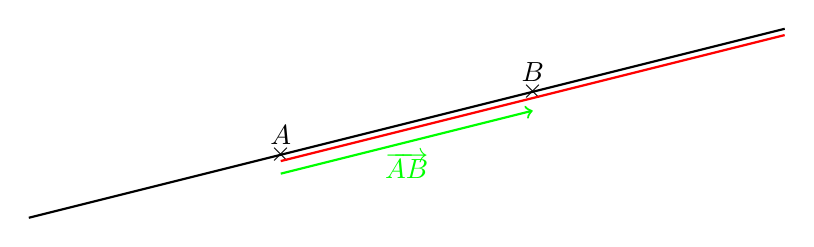
\begin{tikzpicture}[scale=0.8]
\coordinate (A) at (0, 0) ; 
\coordinate (B) at (4, 1) ; 
% Le coef directeur est 1/4 et le vecteur directeur (4 ; 1)     
   
\coordinate (A2) at (0, 0) ; 
\coordinate (B2) at (3, 1) ; 
\coordinate (A3) at (0, 0) ; 
\coordinate (B3) at (3, 1) ; 
\draw[thick] (-4,-1)  -- (8,2) ;
\draw (0,0) node {$\times$} ; \draw (0,0) node [above] {$A$} ;
\draw (4,1) node {$\times$} ; \draw (4,1) node [above] {$B$} ;
    
\draw[thick,red] (0,-0.1)  -- (8,1.9) ;
\draw[thick,green, ->] (0,-0.3)  -- node[midway,below, green]{$ \overrightarrow{AB}$} (4,0.7) ;
\end{tikzpicture}

\begin{itemize}
\item[*] La direction de droite est la direction de la droite $ \left(AB\right) $
\item[*] Le sens sur cete direction est le sens de A vers B, c'est-à-dire le sens de la demi-droite $\left[AB\right)$
\item[*] Le nombre réel positif est la longueur du segment $\left[AB\right]$, c'est-à-dire la distance AB.
\end{itemize}

\subsection{Égalité de 2 vecteurs}

Soient $\overrightarrow{AB}$ et $\overrightarrow{CD}$ deux vecteurs. \\

$\overrightarrow{AB}=\overrightarrow{CD}$ si et seulement si :
\begin{itemize}
\item[*] La direction $(AB) =$ la direction de $(CD)$, c'est-à-dire $(AB)//(CD)$.
\item[*] Le sens de $\left[AB\right) =$ le sens de $\left[CD\right)$
\item[*] La longueur de $[AB] =$ la longueur de $[CD]$
\end{itemize}

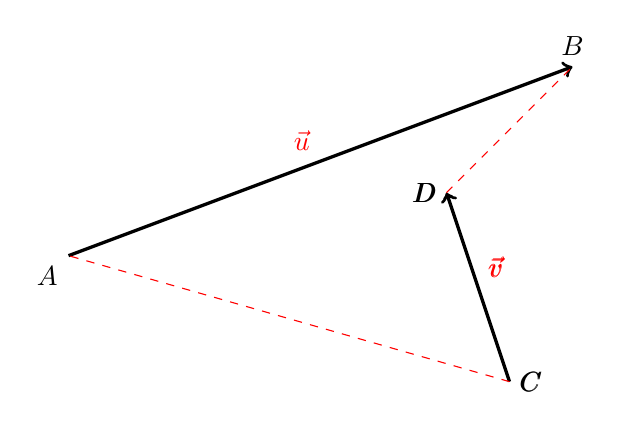
\begin{tikzpicture}[scale=0.8]
\draw[color=black,very thick, ->]
% A(0,0) L'étiquette est à côté de du point.
% Le nom du vecteur u est au dessus à gauche du milieu du trait épais 
(0,2) node [below left] {$A$} --  node[color=red, midway,above left]{$\vec{u}$}
% Le + signifie la translation 
+(8,3) node [above] {$B$} ;
\draw[color=black,very thick,->] (7,0) node [right] {$C$} --  node[color=red, above right]{$\vec{v}$} +(-1,3) node [left] {$D$} ;
\draw[color=black,->] (7,0) node [right] {$C$} --  node[color=red, above right]{$\vec{v}$} +(-1,3) node [left] {$D$} ;
\draw[color=red,dashed] (7,0)  -- (0,2) ;
\draw[color=red,dashed] (6,3)  -- (8,5) ;
\end{tikzpicture}\\
$\overrightarrow{AB} \neq \overrightarrow{CD}$ car $(AB)$ et $(CD)$ ne sont pas parralèles

\newpage



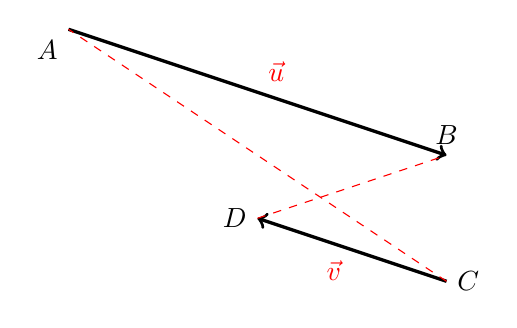
\begin{tikzpicture}[scale=0.8]
\draw[color=black,very thick, ->]
(0,4) node [below left] {$A$} --  node[color=red, midway,above right]{$\vec{u}$}+(6,-2) node [above] {$B$} ;
\draw[color=black,very thick,->] (6,0) node [right] {$C$} --  node[color=red, below left]{$\vec{v}$} +(-3,1) node [left] {$D$} ;
\draw[color=red,dashed] (6,0)  -- (0,4) ;
\draw[color=red,dashed] (3,1)  -- (6,2) ;
\end{tikzpicture}\\


$\overrightarrow{AB} \neq \overrightarrow{CD}$ car $(AB) // (CD)$ mais le sens de $[AB) \neq$ le sens de $[CD)$.

\vspace{1cm}

\begin{tikzpicture}[scale=0.8]
\draw[color=black,very thick, ->]
(5,5) node [below left] {$A$} --  node[color=red, midway,above left]{$\vec{u}$}+(-4,-2) node [above] {$B$} ;
\draw[color=black,very thick,->] (9,5) node [right] {$C$} --  node[color=red, below right]{$\vec{v}$} +(-9,-5) node [left] {$D$} ;
\draw[color=red,dashed] (0,0)  -- (1,3) ;
\draw[color=red,dashed] (5,5)  -- (9,5) ;
\end{tikzpicture}\\

$\overrightarrow{AB} \neq \overrightarrow{CD}$ car $(AB) // (CD)$, le sens de $[AB) = $ le sens de $[CD)$, mais $AB \neq CD$.

\vspace{1cm}

\begin{tikzpicture}[scale=0.8]
\draw[color=black,very thick, ->]
(0,2) node [above left] {$A$} --  node[color=red, midway,above left]{$\vec{u}$}+(8, 2) node [above] {$B$} ;
\draw[color=black,very thick,->] (0,0) node [left] {$C$} --  node[color=red, below right]{$\vec{v}$} +(8, 2) node [right] {$D$} ;
\draw[color=red,dashed] (0,0)  -- (0, 2) ;
\draw[color=red,dashed] (8,2)  -- (8, 4) ;
\end{tikzpicture}\\

$\overrightarrow{AB} = \overrightarrow{CD}$ car $(AB) // (CD)$, le sens de $[AB) = $ le sens de $[CD)$ et $AB = CD$.

$\overrightarrow{u} =\overrightarrow{AB} = \overrightarrow{CD}$

En rouge, le quadrilatère ABDC.

$\overrightarrow{AB} = \overrightarrow{CD} \Longleftrightarrow$ ABDC est un parallélogramme.

Remarques :
\begin{itemize}
\item[*] {\Large $\Longleftrightarrow$} se lit : \og  équivalent à \fg , ou \og  si et seulement si \fg
\item[*] Si $\overrightarrow{AB} = \overrightarrow{CD}$, et ABDC est un parallélogramme, on a aussi :
\begin{itemize}
\item[*]$\overrightarrow{BA} = \overrightarrow{DC}$
\item[*]$\overrightarrow{AC} = \overrightarrow{BD}$
\item[*]$\overrightarrow{CA} = \overrightarrow{DB}$
\end{itemize}
\end{itemize}

\newpage

\subsection{Axiome fondamental}

Soit O un point. 

Soit $\overrightarrow{u}$ un vecteur.

\begin{tikzpicture}[scale=0.8]
\tkzDefPoint [label=left:$O$](0,0){O}
\tkzDrawPoint[size=10,color=black](O)

	\coordinate (M) at (6, 2) ; 

    \draw[very thick,->] (0,0) --  (6,2) node [above] {$M$}  ;
    \draw[thick, ->] (0,-2) -- node[midway,above]{$\vec{u}$} +(6,2);
\end{tikzpicture} \\

Il existe un point M et un seul tel que $\overrightarrow{OM} = \overrightarrow{u}$

\subsection{Addition de vecteurs}

Soit $\vec{u}$ et $\vec{v}$ deux vecteurs.

\begin{tikzpicture}[scale=0.8]
    \coordinate (A) at (0, 0) ; 
    \coordinate (B) at (2, 4) ; 
    \coordinate (C) at (7, 4) ; 	
    \coordinate (C) at (11, 4) ; 	

  \draw[thick,green, ->] (0,0)  --  node[midway,above, green]{$\vec{u}$} +(2,4);
    \draw[thick, ->] (7,4) -- node[midway,above]{$\vec{v}$} +(4,0);

\end{tikzpicture} \\

\subsubsection{Méthode mathématique}

\begin{tikzpicture}[scale=0.8]
    \coordinate (A) at (0, 0) ; 
    \coordinate (B) at (2, 4) ; 
    \coordinate (C) at (2, 4) ; 	
    \coordinate (C) at (6, 4) ; 	
    \draw[thick,green, ->] (0,0) node [below left, black] {$A$} --  node[midway,above, green]{$\vec{u}$} +(2,4) node [above, black] {$B$} ;
    \draw[thick, ->] (2,4) -- node[midway,above]{$\vec{v}$} +(4,0) node [above] {$C$} ;
    \draw[thick,red, ->] (0,0) --  node[midway,below right]{$\vec{u}+\vec{v}$} +(6,4);
\end{tikzpicture}

$\vec{u} + \vec{v} = \overrightarrow{AC}$ \\

$\overrightarrow{AB} + \overrightarrow{BC} = \overrightarrow{AC}$ \\

Ceci s'appelle la \textbf{Relation de Chasles} (Michel Chasles est un mathématicien français (1793-1880)).

\subsubsection{Méthode physique}

\begin{tikzpicture}[scale=0.8]
    \coordinate (A) at (0, 0) ; 
    \coordinate (B) at (2, 4) ; 
    \coordinate (C) at (2, 4) ; 	
    \coordinate (C) at (6, 4) ; 	
    \draw[thick,green, ->] (0,0) node [below left, black] {$O$} --  node[midway,above, green]{$\vec{u}$} +(2,4) node [above, black] {$A$} ;
    \draw[dashed] (2,4) --  +(4,0) node [above] {$C$} ;
    \draw[thick, ->] (0,0) -- node[midway,above]{$\vec{v}$} +(4,0) node [above] {$B$} ;
    \draw[thick,red, ->] (0,0) --  node[midway,below right]{$\vec{u}+\vec{v}$} +(6,4);
    \draw[dashed] (4,0) --  +(2,4) node [above] {$C$} ;
\end{tikzpicture} 

$\vec{u} + \vec{v} = \overrightarrow{OC}$ \\

$\overrightarrow{OA} + \overrightarrow{OB} = \overrightarrow{OC}$ \\

Ceci est \textbf{la règle du parallélogramme}. Le vecteur
$\overrightarrow{OC}$ s'appelle \textbf{la résultante des forces}. \\

\subsection{Conséquences de la relation de Chasles}

\subsubsection{Le vecteur nul}

Soit A un point. \\

Combien vaut le vecteur $\overrightarrow{AA}$ ? \\


$\overrightarrow{AA} + \overrightarrow{AB} = \overrightarrow{AB}$

$ x + a = a $

$ x = 0 $.

Donc $\overrightarrow{AA} = \overrightarrow{0}$ (<-- vecteur nul) \\

\subsubsection{L'opposé d'un vecteur}

Soient A et B deux points.


Combien vaut le vecteur $\overrightarrow{BA}$ ? \\


$\overrightarrow{AB} + \overrightarrow{BA} = \overrightarrow{AA}$

$\overrightarrow{AB} + \overrightarrow{BA} = \overrightarrow{0}$

$ a + x = 0 $

$ x = - a $

Donc $\overrightarrow{BA} = -\overrightarrow{AB}$ (<-- opposé de $\overrightarrow{AB}$

\subsubsection{Soustraction de deux vecteurs}

\begin{tikzpicture}[scale=0.8]
 \draw[thick,green, ->] (0,0)  --  node[midway,below right , green]{$\vec{u}$} +(2,4);
    \draw[thick, ->] (7,4) -- node[midway,above]{$\vec{v}$} +(4,0);
\end{tikzpicture} 

$\overrightarrow{u} - \overrightarrow{v} = \overrightarrow{u}+\left(-\overrightarrow{v}\right)$

\begin{tikzpicture}[scale=0.8]

    \draw[thick, <-] (0,0) -- node[midway,above]{$-\vec{v}$} +(-4,0) node [above] {$C$} ;
    \draw[thick,green, ->] (-2,-4) --  node[midway,below right, green]{$\vec{u}$} +(2,4);
    \draw[thick,red, ->] (-2,-4) --  node[midway,below left]{$\vec{u}-\vec{v}$} +(-2,4);
\end{tikzpicture} 

\subsection{Multiplication d'un vecteur par un nombre réel}

Soit $\overrightarrow{u}$ un vecteur.

Soit $\lambda$ un nombre réel. 

\begin{tikzpicture}[scale=0.8]
 \draw[thick,green, ->] (0,0)  --  node[midway,below right , green]{$\vec{u}$} +(2,4);
\end{tikzpicture} 

Le produit du vecteur $\overrightarrow{u}$ par le nombre réel $\lambda$ est le vecteur noté $\lambda\overrightarrow{u}$ défini par : 

-- La direction de $\left(CD\right) = $ la direction de $\left(AB\right)$, c'est-à-dire $\left(AB\right) // \left(CD\right) $ \\

\begin{tabular}{l|l}

$\lambda > 0 $ & $\lambda < 0$ \\
* Le sens de $\left[CD\right) $ & * le sens de $\left[AB\right) $ \\ 
 $ CD = \lambda AB $ & $ CD = -\lambda AB$ \\
\end{tabular}


\subsubsection{Exemple \no 1}

$\lambda = 3 $

\begin{tikzpicture}[scale=0.6]
\draw[thick,green, ->] (1,2) node [below left] {$A$} --  node[midway,above left, green]{$\vec{u}$} +(1,2) node [above] {$B$} ;
    
\draw[thick,green, ->] (3,0) node [below] {$C$} --  node[midway, below right, green]{$3\vec{u}$} +(3,6) node [above ] {$D$} ;
\draw (4,2) node {$-$} ; \draw (5,4) node {$-$} ; 
\end{tikzpicture}

\subsubsection{Exemple \no 2}

$\lambda = -2 $

\begin{tikzpicture}[scale=0.8]
\draw[thick, ->] (1,2) node [below left] {$A$} --  node[midway,above left]{$\vec{u}$} +(1,2) node [above] {$B$} ;
    
\draw[thick, <-] (3,0) node [below] {$D$} --  node[midway, below right]{$-2\vec{u}$} +(2,4) node [above ] {$C$} ;
\draw (4,2) node {$-$} ; 
\end{tikzpicture}

Et si $\lambda = 0$ ? \\

Alors $0\overrightarrow{u} = \overrightarrow{0}$

\subsection{Notions d'espace vectoriel}

Soient $\overrightarrow{u}$, $\overrightarrow{v}$, et  $\overrightarrow{w}$ trois vecteurs.

Soient $\lambda$ et $\mu$ deux nombres réels. \\

\subsubsection{Relations avec des vecteurs}

\begin{itemize}
\item[*] $\overrightarrow{u} + \overrightarrow{v}$ = $\overrightarrow{v} + \overrightarrow{u}$
\item[*] $\overrightarrow{u} + \left(\overrightarrow{v} + \overrightarrow{w} \right) = \left( \overrightarrow{u} + \overrightarrow{v} \right) + \overrightarrow{w}$
\item[*] $\overrightarrow{u} + \overrightarrow{0} = \overrightarrow{u}$
\item[*] $\overrightarrow{u} + \left(-\overrightarrow{u}\right) = \overrightarrow{0}$
\end{itemize}

\subsubsection{Relations avec des vecteurs et des nombres réels}

\begin{itemize}
\item[*]$1\overrightarrow{u} = \overrightarrow{u}$
\item[*]$\lambda\left(\mu \overrightarrow{u} \right) = \left(\lambda\mu\right)\overrightarrow{u}$
\item[*] $\lambda \times \left( \overrightarrow{u} + \overrightarrow{v}\right) = \lambda \overrightarrow{u} + \lambda \overrightarrow{v}$
\item[*] $\left(\lambda + \mu \right) \overrightarrow{u} = \lambda \overrightarrow{u} + \mu \overrightarrow{u}$
\end{itemize}

\newpage 
\subsection{Vecteurs colinéaires}

\subsubsection{Définition}

Soient $\overrightarrow{u}$ et $\overrightarrow{v}$ deux vecteurs, avec $\overrightarrow{u} \neq \overrightarrow{0}$.

$\overrightarrow{v}$ est colinéaire à $\overrightarrow{u}$ si et seulement si : il existe $\lambda \in \R$ tel que $\overrightarrow{v} = \lambda\overrightarrow{u}$ \\

Exemple :

\begin{tikzpicture}[scale=0.6]
% A(0,0) L'étiquette est à côté de du point.
% Le nom du vecteur u est au dessus à gauche du milieu du trait épais 
\draw[thick, ->] (0,0) node [below left] {$A$} --  node[midway,above left]{$\vec{u}$}
% Le + signifie la translation 
+(2,2) node [above] {$B$} ;

% D(3,0)
\draw[thick, ->] (3,0) node [below] {$D$} --  node[midway, below right]{$\vec{v}$} +(6,6) node [above ] {$C$} ;
% On place deux petites marques pour montrer v = 3u
\draw (5,2) node {$\setminus$} ; 
\draw (7,4) node {$\setminus$} ; 
\end{tikzpicture}

$\overrightarrow{v}$ est coliénaire à $\overrightarrow{u}$ car  $\overrightarrow{v} = 3 \overrightarrow{u}$. \\

\textbf{Remarque}

$\overrightarrow{0}$ est colinéaire à tous les vecteurs du plan. En effet, pour tout vecteur $\overrightarrow{u}$, on a $\overrightarrow{0} = 0 \overrightarrow{u}$ \\

Soient $\overrightarrow{u} \neq \overrightarrow{0}$ et $\overrightarrow{v} \neq \overrightarrow{0}$ tels que $\overrightarrow{v}$ est colinéaire à $\overrightarrow{u}$. Il existe $ \lambda \in \R $ tel que $\overrightarrow{v} = \lambda\overrightarrow{u}$ avec $\lambda \neq 0 $.

On a donc $\overrightarrow{u} = \dfrac{1}{\lambda}\overrightarrow{v}$ et non $\overrightarrow{u} = \dfrac{\overrightarrow{v}}{\lambda}$

\subsubsection{Syntaxe}

On dit que $\overrightarrow{u}$ et $\overrightarrow{v}$ sont colinéaires, ou que $\overrightarrow{v}$ est colinéaire à  $\overrightarrow{u}$. 

\subsubsection{À retenir}

Soient $\overrightarrow{u}$ et $ \overrightarrow{v} $ deux vecteurs 
colinéaires. Il existe un nombre $\lambda \in \R $ tel que $ \overrightarrow{v} = \lambda \overrightarrow{u} $ avec $ \lambda \neq 0$ \\

\begin{tabular}{c|c}

Si $\lambda > 0 $ & Si $\lambda < 0$ \\
$\overrightarrow{u}$ et $\overrightarrow{v}$ sont colinéaires et de même sens & $\overrightarrow{u}$ et $\overrightarrow{v}$ sont colinéaires et de sens contraires.

\end{tabular}

\subsubsection{Points alignés}

Soient A, B et C trois points alignés.\\

A, B et C sont alignés si et seulement si : $ \overrightarrow{AB}$ et $\overrightarrow{AC}$ sont colinéaires.

% Points alignés
\begin{tikzpicture}[scale=0.8]
\draw[thick, ->] (0,0) --  +(5,3)  ;
 \tkzText(0.5,0.3){\textcolor{black}{$\times$}}  % cf ci-dessus
 \tkzText(.5,.7){\textcolor{black}{A}}
 \tkzText(1.5,.9){\textcolor{black}{$\times$}}  % cf ci-dessus
 \tkzText(1.5,1.3){\textcolor{black}{B}}
 \tkzText(4,2.4){\textcolor{black}{$\times$}}  % cf ci-dessus
 \tkzText(3.9,2.8){\textcolor{black}{C}}
\end{tikzpicture}

A, B et C sont alignés car $\overrightarrow{AB}$ et $\overrightarrow{AC}$ sont colinéaires.

\subsubsection{Droites parallèles}

Soient $\left(AB\right)$ et $\left(CD\right)$ deux droites : \\

$\left(AB\right)$ et $\left(CD\right)$ sont parallèles si et seulement si : $\overrightarrow{AB}$ et $\overrightarrow{AC}$ sont colinéaires.

% Droites //
\begin{tikzpicture}[scale=0.8]
% A(0,0) 
\draw[-] (-2,-1) -- +(8,4) ;
\draw[very thick, ->] (0,0) node [below left] {$A$} -- +(4,2) ;
\draw (0,0) node {$\setminus$} ; 
%\draw (2,1) node {$-$} ; 
%\draw (4,2) node {$-$} ; 
%\draw (4,2) node {$\times$} ; 
%\draw (4,2) node {$\times$} ; 
\draw (4,2) node [above]{$B$} ; 
% D(3,0)
\draw[-] (2,-1) -- +(8,4) ;
\draw[very thick, ->] (4,0) node [below] {$C$} --   +(1, .5) node [above ] {$D$} ;
\end{tikzpicture}

$\left(AB\right) // \left(CD\right) $ car $\overrightarrow{CD} = \dfrac{1}{4} \overrightarrow{AB}$

\subsection{Milieu d'un segment}

\subsubsection{Définition}

Soient A et B deux points distincts.

Il existe un point I et un seul tel que $\overrightarrow{IA} + \overrightarrow{IB} = \overrightarrow{0}$, c'est-à-dire $\overrightarrow{AI} = \dfrac{1}{2} \overrightarrow{AB} $

I est le milieu de $\left[AB\right]$

% milieu d'un segmeny
\begin{tikzpicture}[scale=0.8]
\draw[very thick, -] (-.2,0) --  +(6.4,0)  ;
 \tkzText(0,0){\textcolor{black}{$|$}}  % cf ci-dessus
 \tkzText(0,.5){\textcolor{black}{A}}
 \tkzText(3,0){\textcolor{black}{$|$}}  % cf ci-dessus
 \tkzText(3,.5){\textcolor{black}{$I$}}
 \tkzText(6,0){\textcolor{black}{$|$}}  % cf ci-dessus
 \tkzText(6,.5){\textcolor{black}{$B$}}
\draw (1.47,0.09) -- (1.47,-0.09);
\draw (1.54,0.09) -- (1.54,-0.09);
\draw (4.47,0.09) -- (4.47,-0.09);
\draw (4.54,0.09) -- (4.54,-0.09);
\end{tikzpicture}

\subsubsection{Démonstration}

$\overrightarrow{IA} + \overrightarrow{IB} = \overrightarrow{0} $\\

$ \overrightarrow{IA} + \left(\overrightarrow{IA} + \overrightarrow{AB}\right) = \overrightarrow{0} $\\

$ 2\overrightarrow{IA} + \overrightarrow{AB} = \overrightarrow{0} $\\

$ 2\overrightarrow{IA} = -\overrightarrow{AB} $\\

$\overrightarrow{IA} = -\dfrac{1}{2} \overrightarrow{AB} $\\

$ \overrightarrow{AI} = \dfrac{1}{2} \overrightarrow{AB} $\\

\newpage 

\subsection{Centre de gravité d'un triangle}

Soient A, B et C trois points non-alignés.

Il existe un point G et un seul tel que $\overrightarrow{GA} + \overrightarrow{GB} + \overrightarrow{GC} = \overrightarrow{0} $, c'est-à-dire $\overrightarrow{AG} = \dfrac{1}{3} \overrightarrow{AB} + \dfrac{1}{3} \overrightarrow{AC} $ \\

\subsubsection{Démonstration}

$\overrightarrow{GA}+\overrightarrow{BG}+\overrightarrow{GC}=\overrightarrow{0}$\\

$ \overrightarrow{GA} + \left(\overrightarrow{GA} + \overrightarrow{AB} \right) + \left(\overrightarrow{GA} + \overrightarrow{AC}\right) = \overrightarrow{0} $\\

$ 3\overrightarrow{GA} = -\overrightarrow{AB} - \overrightarrow{AC} $\\

$ \overrightarrow{GA} = -\dfrac{1}{3} \overrightarrow{AB} - \dfrac{1}{3} \overrightarrow{AC} $\\

$ \overrightarrow{AG} = \dfrac{1}{3} \overrightarrow{AB} + \dfrac{1}{3} \overrightarrow{AC} $\\

\subsubsection{Propriété fondamentale}

\begin{tikzpicture}[scale=0.5]
\coordinate (G) at (0.2,-0.07) ; 

\draw (6,8) node [above] {$A$} --  (-8.7,-5) node [left] {$B$} -- (8.7,-5) node [right] {$C$}-- (6, 8) ; 
\draw (6,8) -- (0,-5) node [below] {$A'$} ;
\draw (-8.7,-5) -- (7.4,1.5) node [right] {$B'$} ;
\draw (8.7,-5) -- (-1.3,1.5) node [left] {$C'$} ;
\draw (2,-0.7) node [below right] {$G$} ; 

\draw [very thick, ->](6,8) -- +(-14.7/3, -13/3) ; % 1/3 de vec(AB)
\draw [dashed](2, -0.7) -- +(-2.7/3, 13/3) ;       % 1/3 de vec(-AC)
\draw [very thick, ->](6,8) -- +(2.7/3, -13/3) ;   % 1/3 de vec(AC)
\draw [dashed](2, -0.7) -- +(14.7/3, 13/3) ;       % 1/3 de vec(-AB)
\draw [very thick, ->](6,8) -- +(-12/3, -26/3) ;   % 2/3 de vec(AA')
\draw [very thick, red] (4,7.3/2) node {\bf ---} ; % 1/2 de AG 

\end{tikzpicture}

Soit A' le milieu de $\left[BC\right]$

$ \overrightarrow{AG} = \dfrac{1}{3} \overrightarrow{AB} + \dfrac{1}{3} \overrightarrow{AC} $\\

$ \overrightarrow{AG} = \dfrac{1}{3} \left(\overrightarrow{AA'} + \overrightarrow{A'B}\right) + \dfrac{1}{3} \left(\overrightarrow{AA'} + \overrightarrow{A'C} \right) $ \\

$ \overrightarrow{AG} = \dfrac{2}{3} \overrightarrow{AA'} + \dfrac{1}{3} \underbrace{\left(\overrightarrow{A'B} + \overrightarrow{A'C}\right)}_{= \overrightarrow{0} \textrm {car} A' \textrm {est le milieu de} \left[BC\right]} $\\

$ \overrightarrow{AG} = \dfrac{2}{3} \overrightarrow{AA'} $\\

On aussi, avec B' le milieu de $\left[AC\right]$, on a $\overrightarrow{BG} = \dfrac{2}{3} \overrightarrow{BB'} $, et avec C' le milieu de $\left[AB\right]$, on a $\overrightarrow{CG} = \dfrac{2}{3} \overrightarrow{CC'} $

Les trois médianes du triangle sont concourantes en un point, ici G.

\newpage

\subsection{Exercices}

\subsubsection{Exercice \no 0}

Soit ABC un triangle. \\

1. Soit A' le milieu de $\left[BC\right]$. Montrer que $\overrightarrow{AB} + \overrightarrow{AC} = 2\overrightarrow{AA'}$. \\

2. Soient I le milieu de $\left[AB\right]$ et J le milieu de $\left[AC\right]$. Montrer que $\overrightarrow{IJ} = \dfrac{1}{2} \overrightarrow{BC}$.

\begin{tikzpicture}[scale=0.3]
\draw (6,8) node [above] {$A$} --  (-8.7,-5) node [left] {$B$} -- (8.7,-5) node [right] {$C$} -- (6, 8) ; 
\draw [red,->](6,8) -- +(-12, -26) node [midway,below right] {$A'$} node [below] {$G$} ;

\draw [green, ->] (-1.3, 1.5) node [left] {$I$} -- (7.4,1.5) node [right] {$J$} ;

\draw [dashed] (-8.7, -5) -- +(2.7,-13) ;     % ie vec(AC)
\draw [dashed] (8.7, -5) -- +(-14.7,-13) ;     % ie vec(AB)

\end{tikzpicture}

1. $\overrightarrow{AB} + \overrightarrow{AC} = \left(\overrightarrow{AA'} + \overrightarrow{A'B}\right) + \left(\overrightarrow{AA'} + \overrightarrow{A'C}\right) $\\

$ \overrightarrow{AB} + \overrightarrow{AC} = 2 \overrightarrow{AA'} + \underbrace{\overrightarrow{A'B} + \overrightarrow{A'C}}_{= \overrightarrow{0} \textrm{ car } A' \textrm { est le milieu de } \left[BC\right]} $

$ \overrightarrow{AB} + \overrightarrow{AC} = 2 \overrightarrow{AA'} $\\

Donc les diagonales du parallélogramme se coupent en leur milieu. \\

2. $ \overrightarrow{IJ} = \overrightarrow{IA} + \overrightarrow{AJ} $\\

$ \overrightarrow{IJ} = -\overrightarrow{AI} + \overrightarrow{AJ} $\\

$ \overrightarrow{IJ} = -\dfrac{1}{2} \overrightarrow{AB} + \dfrac{1}{2} \overrightarrow{AC} $\\

$ \overrightarrow{IJ} = \dfrac{1}{2} \left(-\overrightarrow{AB} + \overrightarrow{AC} \right) $\\

$ \overrightarrow{IJ} = \dfrac{1}{2} \left(\overrightarrow{BA} + \overrightarrow{AC}\right) $\\

$ \overrightarrow{IJ} = \dfrac{1}{2} \overrightarrow{BC} $
\newpage
\subsubsection{Un superbe exercice}

Soit ABC un triangle.

Soit A' le milieu de $\left[BC\right]$.

Soit G le centre de gravité de ABC.

Soit M un point quelconque.\\

1. Montrer que $ \overrightarrow{MA} + \overrightarrow{MB} + \overrightarrow{MC} = 3\overrightarrow{MA} + 2\overrightarrow{AA'}$

2. Montrer que $ \overrightarrow{MA} + \overrightarrow{MB} + \overrightarrow{MC} = 3\overrightarrow{MG} $

\begin{tikzpicture}[scale=0.7]
\draw (0,8) node [left] {$A$} --  (8,4) node [below] {$B$} -- (12,16) node [right] {$C$} -- (0, 8) ; 
\draw [thick, ->] (0,8) -- +(10,2) node [right] {$A'$} ;   
\draw [dashed] (8,4) -- +(-2,8) ;   
\draw [dashed] (12,16) -- +(-8,-10);   
\draw (20/3, 18/2) node [below] {$G$} ; 

\draw [blue, ->] (0,12) node [left] {$M$} -- +(0,-4) ; 
\draw [green, ->] (0,12) node [left] {$M$} -- +(8,-8) ; 
\draw [violet, ->] (0,12) node [left] {$M$} -- +(12,4) ; 

\draw [thick, blue, ->] (0,12) node [left] {$M$} -- +(0,-12) ; 
\draw [black, ->] (0,0) --  +(20,4) ; 
\draw [red, ->] (0,12) -- +(20, -8) ; 

\draw [green, ->] (0,8) -- +(8,-8) ; 
\draw [violet, ->] (8,0) -- +(12,4) ; 

\end{tikzpicture}

\vspace*{1cm}

\begin{enumerate}


\item $\overrightarrow{MA} + \overrightarrow{MB} + \overrightarrow{MC} = \overrightarrow{MA} + \left(\overrightarrow{MA} + \overrightarrow{AA'} + \overrightarrow{A'B}\right) + \left(\overrightarrow{MA} + \overrightarrow{AA'} + \overrightarrow{A'C}\right) $\\

$ \overrightarrow{MA} + \overrightarrow{MB} + \overrightarrow{MC} = 3\overrightarrow{MA} + 2\overrightarrow{AA'} +$\hspace*{-0.94cm}$ \underbrace{\overrightarrow{A'B} + \overrightarrow{A'C}}_{= \overrightarrow{0} \textrm{ car } A' \textrm{ est le milieu de } \left[BC\right]}$ 

\item  $ \overrightarrow{MA} + \overrightarrow{MB} + \overrightarrow{MC} = \left(\overrightarrow{MG} + \overrightarrow{GA}\right) + \left(\overrightarrow{MG} + \overrightarrow{GB} \right) + \left(\overrightarrow{MG} + \overrightarrow{GC} \right) $\\

$ \overrightarrow{MA} + \overrightarrow{MB} + \overrightarrow{MC} =
3\overrightarrow{MG} + $\hspace*{-1.8cm}$\underbrace{\overrightarrow{GA} + \overrightarrow{GB} + \overrightarrow{GC}}_{=\overrightarrow{0} \textrm{car } G \textrm { est le centre de gravité du triangle } ABC} $

\end{enumerate}
\newpage
\subsubsection{Exercice \no 1}

Soit ABC un triangle.

1. Construire les points M et N définis par : \\

\begin{itemize}
\item[*] $ \overrightarrow{AM} = \dfrac{1}{3} \overrightarrow{AB} + \overrightarrow{AC} $ \\
\item[*] $ \overrightarrow{AN} = 2\overrightarrow{AB} - \dfrac{2}{3} \overrightarrow{AC} $ \\
\end{itemize}

2. Exprimer $\overrightarrow{MN}$ en fonction de $\overrightarrow{AB}$ et de $\overrightarrow{AC}$. \\

3. Montrer que les droites $\left(MN\right)$ et $\left(BC\right)$ sont parallèles. \\

\begin{enumerate}


\item ~   % Le tilde (~) est nécessaire pour que le numéro précède la figure

\begin{tikzpicture}[scale=0.2]
\draw [color=black] (0,0) node [left] {$B'$} --  (6,12) node [below] {$B$} -- (12,24) node [right] {$A$} ; 
\draw [color=violet] (12,24) -- +(+12, -12)  node [right] {$C$} ; 
\draw [color=black] (24,12) -- (6, 12) ; 
\draw (8,16) node {$-$} ;   
\draw (16,20) node {$-$} ;   
\draw (20,16) node {$-$} ;   

\draw [color=green, very thick, ->] (12, 24) -- +(-2,-4) ; 
\draw [color=violet, thick, ->] (10, 20) -- +(12,-12) node [below] {$M$} ; 
\draw [color=magenta, thick, ->] (0, 0) -- +(-8,8) node [below] {$N$} ; 

\draw [color=red, thick, -] (-10, 12) -- (26,12) ; 
\draw [color=red, thick, -] (-10, 8) -- (26,8) ; 

\end{tikzpicture}\\


\item  $\overrightarrow{MN} = \overrightarrow{MA} + \overrightarrow{AN} $\\

$ \overrightarrow{MN} = -\overrightarrow{AM} + \overrightarrow{AN} $\\

$ \overrightarrow{MN} = -\dfrac{1}{3} \overrightarrow{AB} - \overrightarrow{AC} + 2\overrightarrow{AB} - \dfrac{2}{3} \overrightarrow{AC} $\\

$ \overrightarrow{MN} = \dfrac{5}{3} \overrightarrow{AB} - \dfrac{5}{3} \overrightarrow{AC} $\\

$ \overrightarrow{MN} = \dfrac{5}{3} \left(\overrightarrow{AB} - \overrightarrow{AC}\right) $\\

\item  $ \overrightarrow{MN} = \dfrac{5}{3} \left(\overrightarrow{AB} - \overrightarrow{AC} \right)$\\

$ \overrightarrow{MN} = \dfrac{5}{3} \left(\overrightarrow{AB} + \overrightarrow{CA} \right)$\\

$ \overrightarrow{MN} = \dfrac{5}{3} \left(\overrightarrow{CA} + \overrightarrow{AB} \right)$\\

$ \overrightarrow{MN} = \dfrac{5}{3} \left(\overrightarrow{CB} \right)$\\

$ \overrightarrow{MN} = -\dfrac{5}{3} \left(\overrightarrow{BC}\right)$\\

Les vecteurs $\overrightarrow{MN}$ et $\overrightarrow{BC}$ sont colinéaires, donc $\left(MN\right)//\left(BC\right)$
\end{enumerate}
\newpage
\subsubsection{Exercice \no 2}

Soit ABC un triangle.

\begin{enumerate}


\item  Construire les points I, J et K définis par :

\begin{itemize}
\item[*] $\overrightarrow{AI} = \dfrac{1}{3} \overrightarrow{AB}$\\
\item[*] $\overrightarrow{BJ} = \dfrac{1}{2} \overrightarrow{BA} - \dfrac{1}{4} \overrightarrow{BC}$\\
\item[*] $\overrightarrow{CK} = -\overrightarrow{AB} - \dfrac{1}{2} \overrightarrow{BC}$\\
\end{itemize}

\item  Exprimer $\overrightarrow{IJ}$ fonction de $\overrightarrow{AB}$ et de $ \overrightarrow{BC}$. 

Puis, exprimer $\overrightarrow{IK}$ en fonction de $\overrightarrow{AB}$ et de $\overrightarrow{BC}$.

\item  Montrer que les points I, J et K sont alignés.

\end{enumerate}

~

\begin{enumerate}

\item  ~ % (Garder là le tilde) Exercice n°2 

\begin{tikzpicture}[scale=0.3]

\draw [->] (0, 0) node [left] {$B$} --  +(12, 0) node [below] {$C$} ; 
\draw [color=green, <-] (0, 0) -- +(3, 9) node [above] {$A$} ; 
\draw      (3, 9) --  (12, 0); 

\draw [very thick, color=green, ->] (3, 9) -- +(-1, -3) node [left] {$I$} ; 
\draw [->] (3/2, 9/2) -- +(-3, 0) node [above] {$J$} ; 
\draw [color=green, ->] (12, 0) -- +(3, 9); 
\draw [color=violet, ->] (15, 9) -- +(-6, 0) node [above] {$K$} ; 
\draw [color=red] (2, 6) -- +(14, 6) -- +(-7, -3); 

\end{tikzpicture}\\

\begin{multicols}{2}


\item  {\small $\overrightarrow{IJ} = \overrightarrow{IA} + \overrightarrow{AB} + \overrightarrow{BJ} $\\

$\overrightarrow{IJ} = -\dfrac{1}{3} \overrightarrow{AB} + \overrightarrow{AB} + \dfrac{1}{2} \overrightarrow{BA} - \dfrac{1}{4} \overrightarrow{BC} $\\

$\overrightarrow{IJ} = -\dfrac{1}{3} \overrightarrow{AB} + \overrightarrow{AB} - \dfrac{1}{2} \overrightarrow{AB} - \dfrac{1}{4} \overrightarrow{BC} $\\

$ \overrightarrow{IJ} = \dfrac{1}{6} \overrightarrow{AB} - \dfrac{1}{4} \overrightarrow{BC} $\\

Et : $\overrightarrow{IK} = \overrightarrow{IA} + \overrightarrow{AB} + \overrightarrow{BC} + \overrightarrow{CK} $\\

$ \overrightarrow{IK} = -\dfrac{1}{3} \overrightarrow{AB} + \overrightarrow{AB} + \overrightarrow{BC} - \overrightarrow{AB} - \dfrac{1}{2} \overrightarrow{BC} $\\

$ \overrightarrow{IK} = -\dfrac{1}{3} \overrightarrow{AB} + \dfrac{1}{2} \overrightarrow{BC} $\\

\item $\overrightarrow{IK} = \overrightarrow{IB} + \overrightarrow{BC} + \overrightarrow{BA} + \dfrac{1}{2} \overrightarrow{CB} $\\

$ \overrightarrow{IK} = \dfrac{2}{3} \overrightarrow{AB} + \overrightarrow{BC} - \overrightarrow{AB} - \dfrac{1}{2} \overrightarrow{BC} $\\

$ \overrightarrow{IK} = -\dfrac{1}{3} \overrightarrow{AB} + \dfrac{1}{2} \overrightarrow{BC} $\\

On constate que $\overrightarrow{IK} = -2\left(\dfrac{1}{6} \overrightarrow{AB} + \dfrac{1}{2} \overrightarrow{BC}\right) $\\

$ \overrightarrow{IK} = -2\overrightarrow{IJ} $
}\\

Donc les vecteurs $\overrightarrow{IK}$ et $\overrightarrow{IJ}$ sont colinéaires, donc les points I, J et K sont alignés.

\end{multicols} 
\end{enumerate}
\newpage
\subsubsection{Exercice \no 3}

Soit ABC un triangle.

\begin{enumerate}


\item  Construire les points I et J tels que :

\begin{itemize}
\item[*] $\overrightarrow{AI} = -2\overrightarrow{AB}$\\
\item[*] $\overrightarrow{AJ} = - \overrightarrow{AB} + \dfrac{1}{2} \overrightarrow{AC}$\\
\end{itemize}

\item  Montrer que J et le milieu de $\left[IC\right]$
\end{enumerate}



\begin{enumerate}

 \item ~ \\% Exercice n°3 (suite) 
 
\begin{tikzpicture}[scale=.4]

\draw [color=black] (0, 0) node [left] {$B$} --  (6, 6) node [left] {$A$} ; 
\draw [color=green, ->] (6, 6) -- +(4, -6) node [right] {$C$} ; 
\draw (0, 0) --  (10, 0); 
\draw [color=green, ->] (6, 6) -- +(2, -3); 
\draw [color=violet, ->] (6, 6) -- +(12, 12) node [right] {$I$} ; 
\draw [color=red, ->] (10, 0) -- +(8, 18); 
\draw [color=green, ->] (12, 12) -- +(2, -3) node [right] {$J$} ; 
\end{tikzpicture}

\vspace*{1cm}


\item $\overrightarrow{JI} + \overrightarrow{JC} = \left(\overrightarrow{JA} + \overrightarrow{AI}\right) + \left(\overrightarrow{JA} + \overrightarrow{AC}\right) $

$ \overrightarrow{JI} + \overrightarrow{JC} = \overrightarrow{AB} - \dfrac{1}{2} \overrightarrow{AC} + \overrightarrow{AI} +\overrightarrow{AB} - \dfrac{1}{2} \overrightarrow{AC} + \overrightarrow{AC} $

$\overrightarrow{JI} + \overrightarrow{JC} = 2\overrightarrow{AB} + \overrightarrow{AI} $

$ \overrightarrow{JI} + \overrightarrow{JC} = 2\overrightarrow{AB} + \left(-2\right)\overrightarrow{AB} $

$ \overrightarrow{JI} + \overrightarrow{JC} = \overrightarrow{0} $

Donc J est le milieu de $\left[IC\right]$.

\end{enumerate}

\newpage
\subsubsection{Exercice \no 4}

Soit ABC un triangle.

Soient A' le milieu de $\left[BC\right]$, B' le milieu de $\left[AC\right]$, et C' le milieu de $\left[AB\right]$

Soit G le centre de gravité de ABC.

\begin{enumerate}


\item  Exprimer :

\begin{itemize}
\item[*] $\overrightarrow{AB} + \overrightarrow{AC} $ en fonction de $\overrightarrow{AA'}$\\
\item[*] $\overrightarrow{BA} + \overrightarrow{BC}$ en fonction de $\overrightarrow{BB'}$\\
\item[*] $\overrightarrow{CA} + \overrightarrow{CB}$ en fontion de $\overrightarrow{CC'}$\\
\end{itemize}

\item Montrer que $\overrightarrow{AA'} + \overrightarrow{BB'} + \overrightarrow{CC'} = \overrightarrow{0} $

\item  Montrer que $G$ est le centre de gravité du triangle A'B'C'.
\end{enumerate}



\begin{enumerate}

\item ~ 

\begin{tikzpicture}[scale=1]
\draw (0,0) node [left] {$B$} -- (2,4) node [above] {$A$} -- (8,0) node [right] {$C$} -- cycle ;  
\draw [red] (1,2) node [left] {$C'$} -- (5,2) node [right] {$B'$} -- (4,0) node [below] {$A'$} -- cycle ; 
\draw [thick, ->] (2,4) -- (4,0) ; 
\draw [blue, ->] (0,0) -- +(5,2) (4,0) -- +(5,2) ; 
\draw [green, ->] (8,0) -- +(-7,2) (9,2) -- +(-7,2) ; 
\end{tikzpicture}


 $\overrightarrow{AB} + \overrightarrow{AC} = \left(\overrightarrow{AA'} + \overrightarrow{A'B}\right) + \left(\overrightarrow{AA'} + \overrightarrow{A'C}\right) $\\

$ \overrightarrow{AB} + \overrightarrow{AC} = 2\overrightarrow{AA'} + \underbrace{\overrightarrow{A'B} + \overrightarrow{A'C}}_{= \overrightarrow{0} \textrm { car } A' \textrm { est le milieu de } \left[BC\right]}$\\

$\overrightarrow{AB} + \overrightarrow{AC} = 2\overrightarrow{AA'} $\\

Donc $\overrightarrow{BA} + \overrightarrow{BC} = 2\overrightarrow{BB'} $ et $ \overrightarrow{CA} + \overrightarrow{CB} = 2\overrightarrow{CC'} $\\

\item  $\overrightarrow{AA'} + \overrightarrow{BB'} + \overrightarrow{CC'} = \dfrac{1}{2} \left(\overrightarrow{AB} + \overrightarrow{AC} \right) + \dfrac{1}{2} \left(\overrightarrow{BA} + \overrightarrow{BC} \right) + \dfrac{1}{2} \left( \overrightarrow{CA} + \overrightarrow{CB} \right) $\\

$\overrightarrow{AA'} + \overrightarrow{BB'} + \overrightarrow{CC'} = \dfrac{1}{2} \overrightarrow{AB} + \dfrac{1}{2} \overrightarrow{BA} + \dfrac{1}{2} \overrightarrow{AC} + \dfrac{1}{2} \overrightarrow{CA} + \dfrac{1}{2} \overrightarrow{BC} + \dfrac{1}{2} \overrightarrow{CB} $\\

$ \overrightarrow{AA'} + \overrightarrow{BB'} + \overrightarrow{CC'} = \dfrac{1}{2} \overrightarrow{AA} + \dfrac{1}{2} \overrightarrow{AA} + \dfrac{1}{2} \overrightarrow{BB} $

$ \overrightarrow{AA'} + \overrightarrow{BB'} + \overrightarrow{CC'} = \overrightarrow{0} $\\

\item $\overrightarrow{GA'} + \overrightarrow{GB'} + \overrightarrow{GC'} = \left(\overrightarrow{GA} + \overrightarrow{AA'} \right) + \left(\overrightarrow{GB} + \overrightarrow{BB'} \right) + \left(\overrightarrow{GC} + \overrightarrow{CC'} \right) $\\

$ \overrightarrow{GA'} + \overrightarrow{GB'} + \overrightarrow{GC'} = \underbrace{\overrightarrow{GA} + \overrightarrow{GB} + \overrightarrow{GC}}_{=\overrightarrow{0} \textrm { car } G \textrm { est le centre de gravité de }  ABC} + \underbrace{\overrightarrow{AA'} + \overrightarrow{BB'} + \overrightarrow{CC'}}_{=\overrightarrow{0} \textrm { d'après } 2.} $\\

Donc G est le centre de gravité du triangle A'B'C'.
\end{enumerate}
\newpage
\subsubsection{Exercice \no 5}

Soit ABCD un quadrilatère quelconque.

Soit $O$ le point d'intersection de $\left[AC\right]$ et de $\left[BD\right] $

\begin{enumerate}


\item  Construire les points I, J, K et L tels que 

\begin{itemize}
\item[*]$\overrightarrow{OI} = \overrightarrow{OA} + \overrightarrow{OB} $\\
\item [*]$ \overrightarrow{OJ} = \overrightarrow{OB} + \overrightarrow{OC} $\\
\item [*]$ \overrightarrow{OK} = \overrightarrow{OC} + \overrightarrow{OD} $\\
\item[*] $ \overrightarrow{OL} = \overrightarrow{OD} + \overrightarrow{OA} $\\
\end{itemize}

\item  Montrer que $\overrightarrow{IJ} = \overrightarrow{AC}$.

De même, exprimer $\overrightarrow{LK}$ en fonction de $\overrightarrow{AC}$

\item  Montrer qie IJKL est un parallélogramme.
\end{enumerate}

\begin{enumerate}


\item ~

\begin{tikzpicture}[scale=1]
\draw (1,6) node [left] {$D$} -- (6,12) node [above] {$A$} -- (11, 11) node [right] {$B$} -- (9,3) node [below] {$C$} -- cycle ;  

\draw [green, ->]  (7,9) node [right] {$O$} -- +(4,2) ; 
\draw [blue, ->]   (7,9) -- +(2, -6) ; 
\draw [violet, ->] (7,9) -- +(-6, -3) ; 
\draw [->]         (7,9) -- +(-1,3) ; 

\draw [dashed] (7,9) -- (0,9) ;
\draw [dashed] (7,9) -- (10,14) ;
\draw [dashed] (7,9) -- (13,5) ;
\draw [dashed] (7,9) -- (3,0) ;

\draw [green, ->]  (6,12)  -- +(4,2)   node [above] {$I$} ; 
\draw [blue, ->]   (11,11) -- +(2,-6)  node [right] {$J$} ; 
\draw [violet, ->] (9,3)   -- +(-6,-3) node [below] {$K$} ; 
\draw [->]         (1,6)   -- +(-1,3)  node [left] {$L$} ; 

\draw [red] (10,14) -- ++(3, -9) -- ++(-10, -5) -- ++(-3, 9) -- cycle ; 

\end{tikzpicture}

\item  $\overrightarrow{IJ} = \overrightarrow{IO} + \overrightarrow{OJ}$\\

$ \overrightarrow{IJ} = -\left(\overrightarrow{OA} + \overrightarrow{OB}\right) + \left(\overrightarrow{OB} + \overrightarrow{OC}\right) $\\

$ \overrightarrow{IJ} = -\overrightarrow{OA} - \overrightarrow{OB} + \overrightarrow{OB} + \overrightarrow{OC} $\\

$ \overrightarrow{IJ} = \overrightarrow{AO} + \overrightarrow{OC} $\\

$ \overrightarrow{IJ} = \overrightarrow{AC} $\\

De même :\\

$\overrightarrow{LK} = \overrightarrow{LO} + \overrightarrow{OK}$\\

$ \overrightarrow{LK} = -\left(\overrightarrow{OD} + \overrightarrow{OA}\right) + \left(\overrightarrow{OC} + \overrightarrow{OD}\right) $\\

$ \overrightarrow{LK} = -\overrightarrow{AO} - \overrightarrow{OD} + \overrightarrow{OC} + \overrightarrow{OD} $\\

$ \overrightarrow{LK} = \overrightarrow{AO} + \overrightarrow{OC} $\\

$ \overrightarrow{LK} = \overrightarrow{AC} $\\

\item $ \overrightarrow{IJ} = \overrightarrow{LK} $\\

Donc IJKL est un parallélogramme.

\end{enumerate}
\newpage
\subsubsection{Exercice \no 6}

Soit ABCD un parallélogramme de centre O.

\begin{enumerate}

\item  Montrer que $\overrightarrow{OA} + \overrightarrow{OB} + \overrightarrow{OC} + \overrightarrow{OD} = \overrightarrow{0} $

\item  Soient les points E, F, G et H définis par :

\begin{itemize}
\item[*] $\overrightarrow{OE} = \overrightarrow{OA} + \overrightarrow{OB} $\\
\item [*]$ \overrightarrow{OF} = \overrightarrow{OB} + \overrightarrow{OC} $\\
\item [*]$ \overrightarrow{OG} = \overrightarrow{OC} + \overrightarrow{OD} $\\
\item [*]$ \overrightarrow{OH} = \overrightarrow{OD} + \overrightarrow{OA} $\\
\end{itemize}

Montrer que EFGH est un parallélogramme.

\end{enumerate}


\begin{enumerate}

\item ~

\begin{tikzpicture}[scale=0.8]
\draw [color=black] (1.5, 5) node [left] {$D$} -- 
   (7.5, 7) node [above] {$A$} -- 
   (10.5, 3) node [right] {$B$}  --
   (4.5, 1) node [below] {$C$} -- cycle ; 
\draw [color=black, dashed] (0, 2) node [left] {$G$} -- 
   (3, 8) node [above] {$H$} -- 
   (12, 6) node [right] {$E$}  --
   (9, 0) node [below] {$F$} -- cycle ; 
\draw [color=black] (1.5, 5) -- (10.5, 3)  ;  
\draw [color=black] (7.5, 7) -- (4.5, 1)  ;  
\tkzText(6.4,4.2){\textcolor{black}{$0$}} % A côté de l'intersection 
 
\end{tikzpicture}

$\overrightarrow{OA} + \overrightarrow{OB} + \overrightarrow{OC} + \overrightarrow{OD} = \underbrace{\left(\overrightarrow{OA} + \overrightarrow{OB}\right)}_{=\overrightarrow{0} \textrm { car } O \textrm{ est le milieu de }  \left[AC\right]} + \underbrace{\left(\overrightarrow{OB} + \overrightarrow{OD}\right)}_{\overrightarrow{0} \textrm{ car } O \textrm{ est le milieu de}  \left[BD\right]} $

\item  $\overrightarrow{OE} + \overrightarrow{OG} = \overrightarrow{OA} + \overrightarrow{OB} + \overrightarrow{OC} + \overrightarrow{OD} $

$\overrightarrow{OE} + \overrightarrow{OG} = \overrightarrow{0}$ 

Donc O est le milieu de $\left[EG\right]$. \\

De même, $\overrightarrow{OF} + \overrightarrow{OH} = \overrightarrow{OA} + \overrightarrow{OC} + \overrightarrow{OB} + \overrightarrow{OD} $\\

$\overrightarrow{OF} + \overrightarrow{OH} = \overrightarrow{0}$ \\

Donc O est le milieu de $\left[HF\right]$.\\

O est le milieu de $\left[EG\right]$ et de $\left[HF\right]$, donc EFGH est un parallélogramme de centre O.

\end{enumerate}
                   \newpage
\ifdefined\COMPLETE
\else
    \input{./preambule-sacha-utf8.ltx}
    \begin{document}
\fi


\section{Repères du plan}

\subsection{Définition}

Soit O un point.

Soient $\vec{i}$ et $\vec{j}$ deux vecteurs non colinéaires.

% Les petits poids 
\begin{tikzpicture}[scale=0.6]

\draw[thick, ->] (0,0)  --  node[midway,above]{$\vec{i}$}(2,0) ;
\draw[color=green, thick, ->] (0,1)  --  node[midway,above]{$\vec{j}$}(1,2) ;
\tkzDefPoint [label=below left:$O$](6,0){O}
\tkzDrawPoint [color=black,size=5](O)

\draw[thick, ->] (6,0)  --  node[midway,above]{$\vec{i}$}(8,0) ;
\draw[color=green, thick, ->] (6,0)  --  node[midway,above]{$\vec{j}$}(7,1) ;

\end{tikzpicture}

$\left(O, \vec{i}, \vec{J}\right)$ est un repère du plan.

\subsection{Coordonnées d'un point dans un repère}

Soit $\left(O, \vec{i}, \vec{j}\right)$\\

Soit M un point. \\

Il existe un nombre réel x unique et un nombre réel y unique tels que : \\

$ \overrightarrow{OM} = x\vec{i} + y\vec{j} $ \\

On écrit :

\begin{itemize}
\item $x$ est l'abscisse de M dans $\left(O, \vec{i}, \vec{j}\right)$\\
\item $y$ est l'ordonnée de M dans $\left(O,\vec{i}, \vec{j}\right)$\\
\end{itemize}

\textbf{Remarque}

On dit que $x$ et $y$ sont les coordonnées de M dans $\left(O, \vec{i}, \vec{j}\right) $\\

% Le repère oblique 
\begin{tikzpicture}[scale=0.5]

\draw[color=black, very thick, ->] (0,0)  --  node[midway,below]{$\vec{i}$}(2,0) ;
\draw[color=black, very thick, ->] (0,0)  --  node[midway,above]{$\vec{j}$}(1,1) ;
\draw[color=black, ->] (-3,0) --( 15,0) ; 
\tkzText(12,-0.3){\textcolor{black}{Axes des abscisses}}
\draw[color=black, ->] (-3,-3) -- ( 10,10) ; 
\tkzText(7,8){\textcolor{black}{Axes des}}
\tkzText(6,7.5){\textcolor{black}{ordonnées}}
\draw[color=black, thick, ->] (0, 0) -- (8, 0) ; 
\tkzText(4, 0){\textcolor{black}{|}} 
\tkzText(6, 0){\textcolor{black}{|}} 

\draw[color=black, thick, ->] (8, 0) -- (11, 3) ; 
\tkzText(2, 2){\textcolor{black}{-}} 
\tkzText(3, 3){\textcolor{black}{-}} 

\draw[color=black, thick, -] (3, 3) -- (11, 3) ; 
\draw[color=red, very thick, ->] (0, 0) -- (11, 3) ; 

\tkzText(11.3,3.3){\textcolor{black}{M}}
\end{tikzpicture}\\

$M\left(x,y,\right) \textrm{dans} \left(O, \vec{i}, \vec{j}\right) \Longleftrightarrow \overrightarrow{OM} = x\vec{i} + y\vec{j} $\\
\newpage 
Dans la pratique, on utilise un repère orthogonal, ou mieux, un repère orthonormal. Avant, on appelait cela un repère "orthonormé".\\

% Repère orthogonal
\begin{tikzpicture}[scale=.8]
\tkzInit[xmin=-3,xmax=4, ymin=-2, ymax=4]
\tkzDrawXY [noticks]

\draw[color=red, very thick, ->] (0,0)  --  node[midway,below]{$\vec{i}$}(2,0) ;
\draw [color=red, very thick] (0,.4)  -- (.4,.4) -- (.4, 0) ;  
\draw[color=black, very thick, ->] (0,0) node [below left] {$O$} --  node[midway,above left]{$\vec{j}$}(0,1) ;
\end{tikzpicture} \hspace{1cm}
% Repère orthonormal                 <<<<<<<<<<<<<<<<<<<<<<
\begin{tikzpicture}[scale=.8]
\tkzInit[xmin=-3,xmax=4, ymin=-2, ymax=4]
\tkzDrawXY [noticks]

\draw[color=black, very thick, ->] (0,0)  --  node[midway,below]{$\vec{i}$}(1,0) ;
\draw[color=black, very thick, ->] (0,0) node [below left] {$O$} --  node[midway,above left]{$\vec{j}$}(0,1) ;
\draw [color=red, very thick] (0,.4)  -- (.4,.4) -- (.4, 0) ;  
\end{tikzpicture}
\newpage 
\subsection{Milieu d'un segment}

Soit $\left(O,\vec{i}, \vec{j}\right)$ un repère.

Soient $A\left(x_A,y_A \right) $ et $B \left( x_B,y_B \right) $. 

Soit I le milieu de $\left[AB\right]$ \\

On a I $ \left(\underbrace{\dfrac{x_A + x_B}{2}}_{\textrm{Moyenne des abscisses}}, \underbrace{\dfrac{y_A + y_B}{2}}_{\textrm{Moyenne des ordonnées}}\right) $ \\

\subsubsection{Exemple}

\begin{tabular}{ll}
$x_I = \dfrac{x_A + x_B}{2} $ & $y_I = \dfrac{y_A + y_B}{2}$ \\
 & \\
$ x_I = \dfrac{-3 + 7}{2}$ & $y_I = \dfrac{2+6}{2}$ \\
 & \\
$x_I = 2$ & $y_I = 4$ \\
\end{tabular}

Donc $I\left(2,4\right)$

\begin{center}
% Milieu d'un segment
\begin{tikzpicture}[scale=.4]
\tkzInit[xmin=-4,xmax=8, ymin=-4, ymax=10]
\tkzDrawXY [noticks]
\draw[color=black, very thick, ->] (0,0)  --  node[midway,below]{$\vec{i}$}(1,0) ;
\draw[color=black, very thick, ->] (0,0) node [below left] {$O$} --  node[midway,above left]{$\vec{j}$}(0,1) ;

\draw [color=red, thick] (-3,2) node [color=black, above] {$A (-3, 2)$} -- (2,4)
node [color=black, below right] {$I (2, 4)$} -- (7,6)  node [color=black, above] {$B (7, 6)$} ; 
\tkzText(-3,2){\textcolor{black}{$\times$}}
\tkzText(2,4){\textcolor{black}{$\times$}}
\tkzText(7,6){\textcolor{black}{$\times$}}

\tkzDefPoint(-3,0){XA} 
\tkzText(-3,0){\textcolor{black}{|}}
\tkzLabelPoint[color=black,below](XA){$-3$}
\tkzDefPoint(0,2){YA}
\tkzText(0,2){\textcolor{black}{-}}
\tkzLabelPoint[color=black,right](YA){$2$}
\tkzDefPoint(7,0){XB} 
\tkzLabelPoint[color=black,below](7,-.5){$7$}
\tkzText(7,0){\textcolor{black}{|}}
\tkzDefPoint(0,6){YB}
\tkzText(0,6){\textcolor{black}{-}}
\tkzLabelPoint[color=black,right](YB){$6$}

\end{tikzpicture}\\
\end{center}

\subsubsection{Démonstration}

$ \overrightarrow{IA} + \overrightarrow{IB} = \overrightarrow{0} $\\

$ \overrightarrow{IO} + \overrightarrow{OA} + \overrightarrow{IO} + \overrightarrow{OB} = \overrightarrow{0} $\\

$ 2\overrightarrow{IO} = -\overrightarrow{OA} -\overrightarrow{OB} $\\

$ \overrightarrow{IO} = -\dfrac{1}{2} \overrightarrow{OA} - \dfrac{1}{2} \overrightarrow{OB} $\\

$ \overrightarrow{OI} = \dfrac{1}{2} \overrightarrow{OA} + \dfrac{1}{2} \overrightarrow{OB} $\\

$ \overrightarrow{OI} = \dfrac{1}{2} \left(x_A\vec{i} + x_B\vec{j} \right) + \dfrac{1}{2} \left( y_A\vec{i} + y_B\vec{j}\right) $\\

$ \overrightarrow{OI} = \dfrac{x_A + x_B}{2}\vec{i} + \dfrac{y_A + y_B}{2} \vec{j} $


\newpage


\subsection{Centre de gravité d'un triangle}

Soit $\left(O, \vec{i}, \vec{j}\right)$ un repère.

Soient les points :

\begin{itemize}
\item $A\left(x_A,y_A\right)$\\
\item $B\left(x_B,y_B\right)$\\
\item $C\left(x_C,y_C\right)$\\
\end{itemize}
 
 Soit G le centre de gravité de ABC.
 
On a G $ \left(\underbrace{\dfrac{x_A + x_B + x_C}{3}}_{\textrm{Moyenne des abscisses}}, \underbrace{\dfrac{y_A + y_B + y_C}{3}}_{\textrm{Moyenne des ordonnées}}\right) $ \\

\subsubsection{Exemple}

\begin{tabular}{ll}
$x_G = \dfrac{x_A + x_B + x_C}{3} $ & $y_G = \dfrac{y_A + y_B + y_C}{3}$ \\
$ x_G = \dfrac{5 + 1 + 9}{3}$ & $y_G = \dfrac{10 + 2+6}{3}$ \\
$x_G = 5$ & $y_G = 6$ \\
\end{tabular}

Donc $G\left(5,6\right)$\\

% Centre de gravité
\begin{tikzpicture}[scale=.8]
\tkzInit[xmin=-1,xmax=10, ymin=-1, ymax=11]
\tkzDrawXY [noticks]
\draw[color=black, very thick, ->] (0,0)  --  node[midway,below]{$\vec{i}$}(1,0) ;
\draw[color=black, very thick, ->] (0,0) node [below left] {$O$} --  node[midway,above left]{$\vec{j}$}(0,1) ;

\tkzText(1,2){\textcolor{black}{$\times$}}
\tkzText(5,10){\textcolor{black}{$\times$}}
\tkzText(9,6){\textcolor{black}{$\times$}}
\tkzText(5,6){\textcolor{black}{$\times$}}

\tkzDefPoint(5,10){A} 
\tkzDefPoint(1,2){B} 
\tkzDefPoint(9,6){C} 
\tkzDefPoint(5,6){G} 

\tkzText(5,0){\textcolor{black}{|}}
\tkzText(9,0){\textcolor{black}{|}}
\tkzText(0,2){\textcolor{black}{-}}
\tkzText(0,6){\textcolor{black}{-}}
\tkzText(0,10){\textcolor{black}{-}}


\tkzDefPoint(5,0){XA}  \tkzDefPoint(0,10){YA}
\tkzDefPoint(1,0){XB}  \tkzDefPoint(0,2){YB}
\tkzDefPoint(9,0){XC}  \tkzDefPoint(0,6){YC}

\tkzLabelPoint[color=black,below](XA){$5$}
\tkzLabelPoint[color=black,left](YA){$10$}
\tkzLabelPoint[color=black,left](YB){$2$}
\tkzLabelPoint[color=black,below](XC){$9$}
\tkzLabelPoint[color=black,left](YC){$6$}

\draw [color=red, thick] (A)  node [color=black, above ] {$A$} 
-- (B) node  [color=black,below] {$B$}   -- (C) node  [color=black,right] {$C$}   -- cycle ; 

\draw [color=black, dashed] (3,6) -- (9,6) ; 
\draw [color=black, dashed] (5,10) -- (5,4) ; 

\tkzLabelPoint[color=black,above right](G){$G$}

\end{tikzpicture}

\subsubsection{Démonstration}

$ \overrightarrow{GA} + \overrightarrow{GB} + \overrightarrow{GC} = \overrightarrow{0} $\\

$\left( \overrightarrow{GO} + \overrightarrow{OA} \right) + \left(\overrightarrow{GO} + \overrightarrow{OB}\right) + \left(\overrightarrow{GO} + \overrightarrow{OC} \right) = \overrightarrow{0} $\\

$ 3\overrightarrow{GO} + \overrightarrow{OA} + \overrightarrow{OB} + \overrightarrow{OC} = \overrightarrow{0} $\\

$ \overrightarrow{GO} = \dfrac{1}{3} \left(-\overrightarrow{OA} -\overrightarrow{OB} - \overrightarrow{OC} \right) $\\

$ \overrightarrow{GO} = -\dfrac{1}{3} \overrightarrow{OA} -\dfrac{1}{3} \overrightarrow{OB} - \dfrac{1}{3} \overrightarrow{OC} $\\

$ \overrightarrow{OG} = \dfrac{1}{3} \overrightarrow{OA} +\dfrac{1}{3} \overrightarrow{OB} + \dfrac{1}{3} \overrightarrow{OC} $\\

$ \overrightarrow{OG} = \dfrac{1}{3} \left(x_A\vec{i} + y_A\vec{j} \right) +\dfrac{1}{3} \left(x_B\vec{i} + y_B\vec{j} \right) + \dfrac{1}{3} \left(x_C\vec{i} / y_C\vec{j} \right) $\\

$ \overrightarrow{OG} = \dfrac{x_A + x_B + x_C}{3}\vec{i} + \dfrac{y_A + y_B + y_C}{3} \vec{j} $\\

\newpage

\subsection{Coordonnées d'un vecteur défini par un de ses représentants}

Soit $\left( O, \vec{i}, \vec{j}\right)$\\

Soient  $A\left(x_A, y_A\right)$ et $B\left(x_B, y_B\right) $.\\

$\overrightarrow{AB} \left(\begin{array}{c} x_B - x_A\\ y_B - y_A \end{array}\right)$\\

\subsubsection{Exemple}

Soient les points :\\

\begin{minipage}{.4\textwidth}
\begin{itemize}
\item[*] $A\left(-5,-4\right) $\\
\item[*] $B\left(-2,-3\right) $\\
\item[*] $C\left(1,2\right) $\\
\item [*] $D\left(4,3\right) $\\
\end{itemize}
\end{minipage}
\begin{minipage}{.3\textwidth}
$ x_B - x_A = -2 + 5 = 3 $\\

$ y_B - y_A = -3 - (-4) = -3 + 4 = 1 $\\

$ x_D - x_C = 4 - 1 = 3 $\\

$ y_D - y_C = 3 - 2 = 1 $\\
\end{minipage}

\hspace*{1cm} Donc $ \overrightarrow{AB} \left(\begin{array}{c} 3\\ 1 \end{array}\right)$ et $\overrightarrow{CD} \left(\begin{array}{c} 3\\ 1 \end{array}\right)$\\

\begin{center} 
% \vspace*{.1cm} 
% Vecteur 
\begin{tikzpicture}[scale=.4]
\tkzInit[xmin=-6,xmax=7, ymin=-5, ymax=5]
\tkzDrawXY [noticks]
\draw[color=black, very thick, ->] (0,0)  --  node[midway,below]{$\vec{i}$}(1,0) ;
\draw[color=black, very thick, ->] (0,0) node [below left] {$O$} --  node[midway,above left]{$\vec{j}$}(0,1) ;

\tkzDefPoint(-5,-4){A} 
\tkzDefPoint(-2,-3){B} 
\tkzDefPoint(1,2){C} 
\tkzDefPoint(4,3){D} 

\draw [color=red, thick, ->] (A) node [color=black, above] {$A$} -- +(3, 1) node [color=black, above] {$B$} ; 

\draw [color=red, thick, ->] (C) node [color=black, above] {$C$} -- +(3, 1) node [color=black, above] {$D$} ; 
\end{tikzpicture}
\end{center}

$ \overrightarrow{AB} = 3\vec{i} + \vec{j}$\\

On constate que $\overrightarrow{AB} = \overrightarrow{CD}$\\

\subsubsection{Démonstration}

$\overrightarrow{AB} = \overrightarrow{AO} + \overrightarrow{OB} $\\

$ \overrightarrow{AB} = -\overrightarrow{OA} + \overrightarrow{OB} $\\

$ \overrightarrow{AB} = \overrightarrow{OB} - \overrightarrow{OA} $\\

$ \overrightarrow{AB} = \left( x_B \vec{i} + y_B\vec{j} \right) - \left( x_A\vec{i} + y_A\vec{j} \right) $\\

$ \overrightarrow{AB} = \left(x_B - x_A\right) \vec{i} + \left(y_B - y_A\right) \vec{j} $\\
\newpage
\subsection{Exemples de changements de repères}

\subsubsection{Exemple \no 1}

Soit $\left(O,\vec{i}, \vec{j}\right)$ un repère.\

Soit $\Omega\left(-2,1\right)$\\

Soit $\vec{u} \left(\begin{array}{c} 1\\ 1 \end{array}\right) $ et $\vec{v} \left(\begin{array}{c} 1\\ -1 \end{array}\right)$\\

Soit $M\left(1,4\right)$ dans $\left(\Omega,\vec{u}, \vec{v}\right) $\\

Déterminer les coordonnées de M dans $\left(O, \vec{i}, \vec{j}\right)$\\

% Changement de repères
\begin{tikzpicture}[scale=.8]
\tkzInit[xmin=-6,xmax=5, ymin=-5, ymax=7]
\tkzDrawXY [noticks, label={}]

\draw[color=black,thick, ->] (0,0)  --  node[midway,below]{$\vec{i}$}(1,0) ;
\draw[color=black,very thick, ->] (0,0) node [below left] {$O$} --  node[midway,above left]{$\vec{j}$}(0,1) ;

\tkzDefPoint  (-2,1){Omega} 
\tkzDrawPoints (Omega)
\tkzLabelPoint[left](Omega){$\Omega$}

\tkzDefPoint(3, -2){M} 
\tkzDrawPoints(M)
\tkzLabelPoint[right](M){$M$}

\draw [color=black, thick, ->] (-5, -2) -- (5,8) ; 
\draw [color=black, thick, ->] (-5, 4) -- (4, -5) ; 

\draw[color=black,very thick, ->] (-2,1)  --  node[midway,above]{$\vec{u}$}(-1,2) ;
\draw[color=black,very thick, ->] (-2,1)  --  node[midway,below] {$\vec{v}$}(-1,0) ;
\tkzText(0,-1){\textcolor{black}{/}} \tkzLabelPoint[color=black,left](0,-1){$2$}
\tkzText(1,-2){\textcolor{black}{/}}\tkzLabelPoint[color=black,left](1,-2){$3$}
\tkzText(2,-3){\textcolor{black}{/}}\tkzLabelPoint[color=black,left](2,-3){$2$}

\tkzText(0,3){\textcolor{black}{$\setminus$}} \tkzLabelPoint[color=black,left](0,3){$2$}
\tkzText(1,4){\textcolor{black}{$\setminus$}}\tkzLabelPoint[color=black,left](1,4){$3$}
\tkzText(2,5){\textcolor{black}{$\setminus$}}\tkzLabelPoint[color=black,left](2,5){$4$}
\draw [color=orange, dashed] (3,0) -- (3, -2) -- (0, -2) ; 
\draw [color=black, dashed] (-1,2) -- (3, -2) -- (2, -3) ; 
\end{tikzpicture}

On conjecture $M\left(3,2\right)$\\

$\overrightarrow{OM} = \overrightarrow{O \Omega} + \overrightarrow{\Omega M} $\\

$ \overrightarrow{OM} = \left(-2\vec{i} + \vec{j}\right) + \left(\overrightarrow{u} + 4\overrightarrow{v}\right) $\\

$ \overrightarrow{OM} = \left(-2\vec{i} + \vec{j} \right) + \left(\vec{i} + \vec{j} \right) + 4\left(\vec{i} - \vec{j} \right) $\\

$ \overrightarrow{OM} = 3\vec{i} - 2\vec{j} $\\
\newpage
\subsubsection{Exercice \no 2}

Soit $\left(O, \vec{i}, \vec{j}\right)$ un repère.\\

Soit $\Omega\left(3,2\right)$\\

Soit $\vec{u} \left(\begin{array}{c} 1\\ 2 \end{array}\right)$ et $\vec{v} \left(\begin{array}{c} -2\\ -1 \end{array}\right)$.\\

Soit $M\left(4,3\right)$ dans $\left(\Omega, \vec{u}, \vec{v}\right)$.\\

Déterminer les coordonnées de M dans $\left(O,\vec{i}, \vec{j}\right)$\\

% Ex2 
\begin{tikzpicture}[scale=.6]
\tkzInit[xmin=-4,xmax=5, ymin=-5, ymax=7]
\tkzLabelX[text=bistre] \tkzLabelY[text=bistre]
\tkzRep[xlabel=$\vec{i}$, ylabel=$\vec{j}$]
\tkzDrawXY [text=black]


\tkzDefPoint  (3,2){Omega} 
\tkzDrawPoints (Omega)
\tkzLabelPoint[below right](Omega){$\Omega$}

\tkzDefPoint(1, 7){M} 
\tkzDrawPoints(M)
\tkzLabelPoint[right](M){$M$}

\draw [color=black, thick, ->] (-7, -3) -- (11,6) ; 
\draw [color=black, thick, ->] (-1, -6) -- (8, 12) ; 

\draw[color=black,very thick, ->] (Omega)  --  node[midway,above]{$\vec{u}$} +(1,2) ;
\draw[color=black,very thick, ->] (Omega)  --  node[midway,below] {$\vec{v}$} +(-2,-1) ;

\draw  [color=black, dashed] (-3, -1) -- (1,7) -- (7,10) ; 

\tkzText(5,3){\textcolor{black}{$\setminus$}} \tkzLabelPoint[color=bistre,below right](5, 3){$-1$}
\tkzText(7,4){\textcolor{black}{$\setminus$}} \tkzLabelPoint[color=bistre,below right](7, 4){$-2$}
\tkzText(-3,-1){\textcolor{black}{$\setminus$}}\tkzLabelPoint[color=bistre,below](-3,-1){$3$}


\tkzText(5,6){\textcolor{black}{$-$}} \tkzLabelPoint[color=bistre,left](5,6){$2$}
\tkzText(6,8){\textcolor{black}{$-$}} \tkzLabelPoint[color=bistre,left](6,8){$3$}
\tkzText(7,10){\textcolor{black}{$-$}} \tkzLabelPoint[color=bistre,left](7,10){$4$}

\end{tikzpicture}

On conjecture $M\left(1,7\right)$ dans $\left(O, \vec{i}, \vec{j}\right) $\\

$\overrightarrow{OM} = \overrightarrow{O \Omega} + \overrightarrow{\Omega M} $\\

$ \overrightarrow{OM} = \left(3\vec{i} + 2\vec{j}\right) + \left(4\overrightarrow{u} + 3\overrightarrow{v}\right) $\\

$ \overrightarrow{OM} = \left(3\vec{i} + 2\vec{j} \right) + 4\left(\vec{i} + 2\vec{j} \right) + 3\left(-2\vec{i} - \vec{j} \right) $\\

$ \overrightarrow{OM} = \vec{i} + 7\vec{j} $\\

Donc $M\left(1,7\right)$\\

\newpage

%    \usepackage{variations}

\ifdefined\COMPLETE
\else
    \end{document}
\fi                    \newpage
\ifdefined\COMPLETE
\else
    \input{./preambule-sacha-utf8.ltx}
    \begin{document}
\fi



\section{Bases du plan}

\subsection{Définition}

Soit $\left(O, \vec{i}, \vec{j}\right)$ un repère du plan.

$\left(\vec{i}, \vec{j}\right)$ est une base du plan.

\subsection{Coordonnées d'un vecteur dans une base}

Soit $\left(\vec{i}, \vec{j}\right)$.

Soit $\vec{u}$ un vecteur. \\

Il existe un nombre réel $x$ unique et un nombre réel $y$ unique tels que $\vec{u} = x\vec{i} + y\vec{j}$.

On écrit $\vec{u}\left(\begin{array}{c} x\\ y \end{array}\right)$

$x$ est la première coodonnée (ou composante) de $\vec{u}$.

$ y$ est la deuxième coodonnée (ou composante) de $\vec{v}$

$\vec{u}\left(\begin{array}{c} x\\ y \end{array}\right)$ dans $\left(\vec{i}, \vec{j}\right) \Longleftrightarrow \vec{u} = x\vec{i} + y\vec{i}$

\subsection{Coordonnées de la somme de deux vecteurs et coordonnées du produit d'un vecteur par un nombre réel}

Soit $\left(\vec{i}, \vec{j}\right)$ une base.

Soit $\vec{u}\left(\begin{array}{c} x\\ y \end{array}\right)$ et $\overrightarrow{u'}\left(\begin{array}{c} x'\\ y' \end{array}\right)$

Soit $ \lambda \in \R$.

$\vec{u} + \overrightarrow{u'}\left(\begin{array}{c} x+x'\\ y+y' \end{array}\right)$ et $\lambda \vec{u}\left(\begin{array}{c} \lambda x\\\lambda y \end{array}\right)$

\subsubsection{Exemple}

Soient $\vec{u}\left(\begin{array}{c} 4\\ -2 \end{array}\right)$ et $\vec{v}\left(\begin{array}{c} 2\\ 6 \end{array}\right)$

% Ex 
\begin{tikzpicture}[scale=.4]
\tkzInit[xmin=-3,xmax=13, ymin=-7, ymax=7]
\tkzRep[xlabel=$\vec{i}$, ylabel=$\vec{j}$]
\tkzDrawXY [noticks]%, label={}]


\draw [color=violet, thick, ->] (0,0) -- +(2,6) ; 
\draw [color=red, thick, ->] (0, 0 ) -- +(6, 4) ; 
\draw [color=black, very thick, ->] (0, 0 ) -- +(4, -2) ; 
\draw [color=black, thick, ->] (0, 0 ) -- +(12, -6) ; 

\tkzText(0,-6){\textcolor{black}{-}}\tkzLabelPoint[color=bistre,left](0, -6){$-6$}
\tkzText(0,-2){\textcolor{black}{-}}\tkzLabelPoint[color=bistre,left](0, -2){$-2$}
\tkzText(0,4){\textcolor{black}{-}} \tkzLabelPoint[color=bistre,left](0,4){$4$}
\tkzText(0, 6){\textcolor{black}{-}} \tkzLabelPoint[color=bistre, left](0, 6){$6$}



\tkzText(2,0){\textcolor{black}{|}} \tkzLabelPoint[color=bistre,below](2,0){$2$}
\tkzText(4,0){\textcolor{black}{|}} \tkzLabelPoint[color=bistre,below](4,0){$4$}
\tkzText(6,0){\textcolor{black}{|}} \tkzLabelPoint[color=bistre,below](6,0){$6$}
\tkzText(12,0){\textcolor{black}{|}} \tkzLabelPoint[color=bistre,below](12,0){$12$}

\draw[color=black, dashed] (2,6) -- (6, 4) -- (4, -2) ; 

\end{tikzpicture}

On a $\vec{u} + \vec{v}\left(\begin{array}{c} 6\\ 4 \end{array}\right)$ et $ 3 \vec{u}\left(\begin{array}{c} 12\\ -6 \end{array}\right)$
\newpage
\subsubsection{Démonstration} 

1. $\vec{u} + \overrightarrow{u'} = \left(x\vec{i} + y\vec{i}\right) + \left(x'\vec{i} + y'\vec{j}\right) $

$ \vec{u} + \overrightarrow{u'} = \left(x+x'\right) \vec{i} + \left(y + y'\right)\vec{j} $

$\lambda \vec{u} = \lambda \left(x\vec{i} + y\vec{j}\right)$

$\lambda \vec{u} = \lambda x\vec{i} + \lambda y\vec{j} $

\subsection{Vecteurs colinéaires}

Soit $\left(\vec{i}, \vec{j}\right)$.

\subsubsection{Notion de déterminant}

Soit $\vec{u}\left(\begin{array}{c} a\\ b \end{array}\right)$ et $\vec{v}\left(\begin{array}{c} c\\ d \end{array}\right)$

Par définition, on appelle le déterminant de $\vec{u}$ et de $\vec{v}$ : $\det\left(\vec{u}, \vec{v}\right) = \left| \begin{array}{cc}  a & c \\ b & d  \\ \end{array} \right| = ad- bc $

\subsubsection{Exemple \no 1}

Soient $\vec{u}\left(\begin{array}{c} 2\\ 1 \end{array}\right)$ et $\vec{v}\left(\begin{array}{c} 4\\ 5 \end{array}\right)$

$\det\left(\vec{u}, \vec{v}\right) = \left| \begin{array}{cc}  2 & 4 \\ 1 & 5  \\ \end{array} \right| = 10 - 4 = 6 $

\subsubsection{Exemple \no 2}

Soient $\vec{u}\left(\begin{array}{c} 8\\ -6 \end{array}\right)$ et $\vec{v}\left(\begin{array}{c} -4\\ 3 \end{array}\right)$

$\det\left(\vec{u}, \vec{v}\right) = \left| \begin{array}{cc}  8 & -4 \\ -6 & 3  \\ \end{array} \right| = 24 - 24 = 0 $

$\vec{v} = -\dfrac{1}{2} \vec{u} $

\subsubsection{Condition de colinéarité de deux vecteurs}

Soient $\vec{u} \neq \overrightarrow{0} $ et $ \vec{v} \neq \overrightarrow{0} $

$\vec{u}$ et $ \vec{v}$ sont colinéaires $\Longleftrightarrow det\left(\vec{u}, \vec{v}\right) = 0 $
\newpage 
\subsubsection{Démonstration}

\textbf{Sens gauche-droite}

Soient $\vec{u}$ et $ \vec{v}$ deux vecteurs colinéaires.

$\vec{u}\left(\begin{array}{c} a\\ b \end{array}\right)$ et $\vec{v}\left(\begin{array}{c} c\\ d \end{array}\right)$

Il existe $\lambda \in \R$ tel que $\vec{v} = \lambda \vec{u} $

On a alors : $\vec{u}\left(\begin{array}{c} a\\ b \end{array}\right)$ et $\vec{v}\left(\begin{array}{c} \lambda a\\ \lambda b \end{array}\right)$

$\det\left(\vec{u}, \vec{v}\right) = \left| \begin{array}{cc}  a & \lambda a \\ b & \lambda b  \\ \end{array} \right| = a \left(\lambda b\right) - b \left(\lambda a\right)= 0 $

\textbf{Sens droite-gauche}

Soient $\vec{u}$ et $\vec{v}$ deux vecteurs colinéaires tels que $\det(\vec{u}, \vec{v})=0$

$\vec{u}\left(\begin{array}{c} a\\ b \end{array}\right)$ et $\vec{v}\left(\begin{array}{c} c\\ d \end{array}\right)$ \\

L'un au moins des 2 nombres réels $a$ et $b$ n'est pas nul car $\vec{u} \neq \overrightarrow{0} $

Supposons par exemple $a \neq 0$ et posons $\lambda = \dfrac{c}{a}$ et $c = \lambda a$.

$\det (\vec{u}, \vec{v}) = 0$

$\left| \begin{array}{cc}  a & c \\ b & d  \\ \end{array} \right| = 10 - 4 = 6 $

$ad - bc = 0$

$ad - b\left(\lambda a \right) = 0 $

$ a \left( d - \lambda b\right) = 0 $ \\

\begin{tabular}{lll}
$ \underbrace{a = 0}_{\textrm{Impossible}}$ & ou & $d - \lambda b = 0$ \\
 & & $ d = \lambda b $ \\
  
\end{tabular}

Conclusion :

\begin{itemize}
\item $ c = \lambda a $
\item $ d = \lambda b$
\end{itemize}

Donc $\vec{v}\left(\begin{array}{c} \lambda a\\ \lambda b \end{array}\right)$, et $\vec{v}$ est colinéaire à $\vec{u}$.
\newpage
\subsection{Exercices}

\subsubsection{Exercice \no 1}

Soit ABC un triangle.

Soit A' le milieu de $\left[BC\right]$

Soit G le centre de gravité de ABC.

On se place dans le repère $\left(A, \overrightarrow{AB}, \overrightarrow{AC}\right)$

Déterminer les coordonnées de A' dans $\left(A, \overrightarrow{AB}, \overrightarrow{AC}\right)$, puis les coordonnées de G dans $\left(A, \overrightarrow{AB}, \overrightarrow{AC}\right)$.\\

% exercice 1
\begin{tikzpicture}[scale=0.4]
\coordinate (G) at (0.2,-0.07) ; 

\draw (6,8) node [above] {$A$} --  (-8.7,-5) node [left] {$B$} -- (8.7,-5) node [right] {$C$}-- (6, 8) ; 
\draw [dashed] (6,8) -- (0,-5) node [below] {$A'$} ;
\draw [dashed](-8.7,-5) -- (7.4,1.5) node [right] {$B'$} ;
\draw [dashed](8.7,-5) -- (-1.3,1.5) node [left] {$C'$} ;
\draw (2,-0.7) node [below right] {$G$} ; 

\end{tikzpicture}\\

$\overrightarrow{AA'} = \dfrac{1}{2} \overrightarrow{AB} + \dfrac{1}{2}\overrightarrow{AC}$\\

Donc $A'\left(\dfrac{1}{2}, \dfrac{1}{2}\right)$\\

$\overrightarrow{AG} = \dfrac{1}{3} \overrightarrow{AB} + \dfrac{1}{3}\overrightarrow{AC}$\\

Donc $G\left(\dfrac{1}{3}, \dfrac{1}{3}\right)$\\

\textbf{Remarque}\\

$A\left(0,0\right) \textrm{car} \overrightarrow{AA} = 0\overrightarrow{AB} + 0\overrightarrow{AC}$\\

$B\left(1,0\right) \textrm{car} \overrightarrow{AB} = 1\overrightarrow{AB} + 0\overrightarrow{AC}$\\

$C\left(0,1\right) \textrm{car} \overrightarrow{AC} = 0\overrightarrow{AB} + 1\overrightarrow{AC}$\\

\newpage
\subsubsection{Exercice \no 2}

Soit $\left(O,\vec{i}, \vec{j}\right)$ un repère. 

Soient les points $A\left(4,2\right)$, $B\left(-4,-4\right)$, $C\left(2,-8\right)$, $D\left(10,-2\right)$.


1.  Montrer par 2 méthodes que ABCD est un parallélogramme.

\vspace*{-9cm}
\begin{tikzpicture}[scale=.6]
\tkzInit[xmin=-5,xmax=12, ymin=-9, ymax=4]
\tkzDrawXY [color=black, noticks] 
\tkzRep[xlabel=$\vec{i}$, ylabel=$\vec{j}$]
\tkzLabelPoint[color=bistre,below left](0,0){$0$}

\tkzDefPoint (4,2){A} \tkzDefPoint (-4, -4){B} \tkzDefPoint (2, -8){C}
\tkzDefPoint (10, -2){D} \tkzDefPoint (3,-3){I}

\draw [color=black, thick] (A) node [above] {$A$}-- 
(B) node [below] {$B$} -- (C) node [below right] {$C$}-- (D) node [below right] {$D$} -- cycle ;   

\draw[color=black] (A) -- (C);  
\draw[color=black] (B) -- (D) ;

\tkzLabelPoint[color=black, below left](I){$I$}

\tkzText(-4,0){\textcolor{bistre}{|}} \tkzLabelPoint[color=bistre, below](-4,0){$-4$}
\tkzText(4,0){\textcolor{bistre}{|}} \tkzLabelPoint[color=bistre, below](4,0){$4$}
\tkzText(10,0){\textcolor{bistre}{|}} \tkzLabelPoint[color=bistre, below](10,0){$10$}
\tkzText(0,-8){\textcolor{bistre}{-}} \tkzLabelPoint[color=bistre, right](0,-8){$-8$}
\tkzText(0, -4){\textcolor{bistre}{-}}  \tkzLabelPoint[color=bistre, left](0,-4){$-4$}
\tkzText(0, -2){\textcolor{bistre}{-}}  \tkzLabelPoint[color=bistre, left](0,-2){$-2$}
\tkzText(0, 22){\textcolor{bistre}{-}}  \tkzLabelPoint[color=bistre, left](0,2){$2$}
\end{tikzpicture}\\

\textbf{Première méthode} \\

$x_B - x_A = -4 - 4 = -8 $

$y_B - y_A = -4 - 2 = -6 $

Donc $\overrightarrow{AB}\left(\begin{array}{c} -8\\ -6 \end{array}\right)$ \\

$x_C - x_D = 2 - 10 = -8 $

$ y_C - y_D = -8 - \left(-2\right) = -6 $

Donc $\overrightarrow{DC}\left(\begin{array}{c} -8\\ -6 \end{array}\right)$ 

On a $\overrightarrow{AB} = \overrightarrow{DC}$ donc ABCD est un parallélogramme. \\

\textbf{Deuxième méthode}\\

Soit I le milieu de $\left(AC\right)$ : \\

\begin{itemize}
\item[*] $x_I = \dfrac{x_A + x_C}{2} = \dfrac{4+2}{2} = 3 $\\
\item[*] $ y_I = \dfrac{y_A + y_C}{2} = \dfrac{2 - 8}{2} = -3 $\\
\end{itemize}

Donc $I\left(3,-3\right)$ \\

Soit J le milieu de $\left(BD\right)$ : \\

\begin{itemize}
\item $x_J = \dfrac{x_B + x_D}{2} = \dfrac{-4+10}{2} = 3 $\\
\item $ y_J = \dfrac{y_B + y_D}{2} = \dfrac{-4 -2}{2} = -3 $\\
\end{itemize}

Donc $J\left(3,-3\right)$\\

$I = J$, donc ABCD est un parallélogramme.  \\

2. Soient $A\left(-6,0\right)$, $ B\left(-1,3\right)$, $C\left(7,-5\right)$, et $D\left(x,y\right)$

Déterminer x et y pour que ABCD soit un parallélogramme. (2 méthodes) \\

% Première méthode
\begin{tikzpicture}[scale=.5]

\tkzInit[xmin=-7,xmax=8, ymin=-9, ymax=4]
\tkzRep[xlabel=$\vec{i}$, ylabel=$\vec{j}$]
\tkzDrawXY [color=black, noticks]%, label={}]
\tkzLabelPoint[color=bistre,below left](0,0){$0$}

\draw [color=black]  (-6, 0) node [above] {$A$} -- (-1, 3) node [above] {$B$} -- (7, -5) node [right] {$C$} -- (2, -8) node [below] {$D$} -- cycle  ; 
\draw [color=black] (-6,0) -- (.5, -2.5) node [above] {$I$} -- (7, -5) ; 
\tkzDrawPoint[color=black](.5,-2.5) 
\tkzLabelPoint[color=bistre, below left](-6,0){$-6$}
\tkzText(-1,0){\textcolor{bistre}{|}} \tkzLabelPoint[color=bistre, below left](-1,0){$-1$}
\tkzText(7,0){\textcolor{bistre}{|}} \tkzLabelPoint[color=bistre, below left](7,0){$7$}
\tkzText(0,-5){\textcolor{bistre}{-}} \tkzLabelPoint[color=bistre, left](0,-5){$-5$}
\tkzText(0, 3){\textcolor{bistre}{-}}  \tkzLabelPoint[color=bistre, left](0,3){$3$}

\end{tikzpicture}

$D\left(2,-8\right)$ On conjecture que $D\left(2,-8\right)$.\\

\textbf{Première méthode}\\

$x_B - x_A = -1 -\left(-6\right) = 5 $

$ y_B - y_A = 3 - 0 = 3 $\\

Donc $\overrightarrow{AB}\left(\begin{array}{c} 5\\ 3 \end{array}\right)$

$x_C - x_D = 7 - x$

$ y_C - y_D = -5 - y $ \\


Donc $\overrightarrow{DC}\left(\begin{array}{c} 7-x\\ -5-y \end{array}\right)$


\begin{tabular}{lll}
$ABCD$ est un parallélogramme & $\Longleftrightarrow$ & $\overrightarrow{AB} = \overrightarrow{DC} $ \\
& $\Longleftrightarrow$ & $ \begin{cases} 7 - x = 5 \\ -5 - y = 3 \end{cases}$ \\
& $ \Longleftrightarrow$ & $ \begin{cases} -x = -2 \\ -y = 8 \end{cases} $ \\
& $\Longleftrightarrow$ & $ \begin{cases}x = 2 \\ y = -8 \end{cases} $ \\
\end{tabular}

Donc $D\left(2,-8\right)$\\

\textbf{Deuxième méthode}\\
Soient I le milieu de $ \left[AC\right] $ et J le milieu de $\left[BD\right]$.\\

$x_I = \dfrac{-6 + 7}{2} = \dfrac{1}{2} $\\

$ y_I = \dfrac{0-5}{2} = -\dfrac{5}{2} $\\

$ x_J = \dfrac{-1 + x}{2} $\\

$ y_J = \dfrac{3 + y}{2} $\\

\begin{tabular}{lll}
$ABCD$ est un parallélogramme & $\Longleftrightarrow$ & I = J \\
& $\Longleftrightarrow$ & $ \begin{cases} \dfrac{-1 + x}{2} = \dfrac{1}{2} \\ 
              \\
\dfrac{3 + y}{2} = -\dfrac{5}{2} \end{cases}$ \\
&& \\
& $ \Longleftrightarrow$ & $ \begin{cases} -1 + x = 1 \\ 3 + y = -5 \end{cases} $ \\
&& \\
& $\Longleftrightarrow$ & $ \begin{cases} x = 2 \\ y = -8 \end{cases} $ \\
\end{tabular}


\newpage
\subsubsection{Exercice \no 3}

Soit $\left(O, \vec{i}, \vec{j}\right)$ un repère. \\

1. Soient $A\left(5,3\right)$, $B\left(8,5\right)$, $C\left(13,9\right)$.

Les points A, B et C sont-il alignés ?

% Exercice n°3
\begin{tikzpicture}[scale=.6]

\tkzInit[xmin=-2,xmax=15, ymin=-2, ymax=9]
\tkzDrawXY [color=black, noticks] 
\tkzLabelPoint[color=bistre,below left](0,0){$0$}
 
\draw [color=black] (-1,-1) -- (14,9) ; 
\tkzDrawPoint[color=black](5,3) \tkzLabelPoint[color=black, above](5,3){$A$} 
\tkzDrawPoint[color=black](8, 5) \tkzLabelPoint[color=black, above](8,5){$B$}
\tkzDrawPoint[color=black](13,8) \tkzLabelPoint[color=black, below](13,8){$C$}  

\tkzText(5,0){\textcolor{bistre}{|}} \tkzLabelPoint[color=bistre, below](5,0){$5$}
\tkzText(8,0){\textcolor{bistre}{|}} \tkzLabelPoint[color=bistre, below](8,0){$8$}
\tkzText(13,0){\textcolor{bistre}{|}} \tkzLabelPoint[color=bistre, below](13,0){$13$}
\tkzText(0,3){\textcolor{bistre}{-}} \tkzLabelPoint[color=bistre, left](0,3){$3$}
\tkzText(0, 5){\textcolor{bistre}{-}}  \tkzLabelPoint[color=bistre, left](0,5){$5$}
\tkzText(0, 8){\textcolor{bistre}{-}}  \tkzLabelPoint[color=bistre, left](0,8){$8$}

\end{tikzpicture}

$x_B - x_A = 8 - 5 = 3 $

$ y_B - y_A = 5 - 3 = 2 $

Donc $\overrightarrow{AB}\left(\begin{array}{c} 3\\ 2 \end{array}\right)$ \\

$ x_C - x_A = 13 - 5 = 8 $

$ y_C - x_A = 8 - 3 = 5 $

Donc $\overrightarrow{AC}\left(\begin{array}{c} 8\\ 5 \end{array}\right)$

$\det\left(\overrightarrow{AB}, \overrightarrow{AC}\right) = \left| \begin{array}{cc}  3 & 8 \\ 2 & 5  \\ \end{array} \right| = 15- 16 = -1 $

$\det\left(\overrightarrow{AB}, \overrightarrow{AC}\right) \neq 0 $

$\overrightarrow{AB}$ et $ \overrightarrow{AC}$ ne sont pas colinéaires. Donc les points A, B et C ne sont pas alignés. \\

\newpage

2. Soient $A\left(-4,5\right)$, $B\left(4,1\right)$, $C\left(x,-1\right)$.

Déterminer $x$ pour que les points A, B et C soient alignés.

$\overrightarrow{AB}\left(\begin{array}{c} 8\\ -4 \end{array}\right)$ et $\overrightarrow{AC}\left(\begin{array}{c} x+4\\ -6 \end{array}\right)$

\begin{tabular}{lll}
A, B et C sont alignés & $\Longleftrightarrow $ & $\overrightarrow{AB}$ et $\overrightarrow{AC}$ sont colinéaires. \\
& $\Longleftrightarrow$ & $\det\left(\overrightarrow{AB}, \overrightarrow{AC} \right) = 0 $ \\
& $\Longleftrightarrow$ & $-48 + 4\left(x+4\right) = 0$ \\
& $\Longleftrightarrow$ & $4\left(x+4\right) = 48 $ \\
& $ \Longleftrightarrow$ & $4x + 16 = 48$ \\
& $ \Longleftrightarrow$ & $4x = 32$ \\
& $\Longleftrightarrow $ & $x = 8 $ \\
\end{tabular}

Donc $C\left(8, -1\right)$

% Exercice n°3 suite .
\begin{tikzpicture}[scale=.6]

\tkzInit[xmin=-7,xmax=13, ymin=-4, ymax=6]
\tkzDrawXY [color=black, noticks] 
\tkzLabelPoint[color=bistre,below left](0,0){$0$}
 
\draw [color=black] (-6,6) -- (12,-3) ; 
\tkzDrawPoint[color=black](-4,5) \tkzLabelPoint[color=black, above](-4,5){$A$} 
\tkzDrawPoint[color=black](4, 1) \tkzLabelPoint[color=black, above](4,1){$B$}
\tkzDrawPoint[color=black](8,-1) \tkzLabelPoint[color=black, below](8,-1){$C$}  

\tkzText(-4,0){\textcolor{bistre}{|}} \tkzLabelPoint[color=bistre, below](-4,0){$-4$}
\tkzText(4,0){\textcolor{bistre}{|}} \tkzLabelPoint[color=bistre, below](4,0){$4$}
\tkzText(8,0){\textcolor{bistre}{|}} \tkzLabelPoint[color=bistre, below](8,0){$8$}
\tkzText(0,-1){\textcolor{bistre}{-}} \tkzLabelPoint[color=bistre, left](0,-1){$-1$}
\tkzText(0, 1){\textcolor{bistre}{-}}  \tkzLabelPoint[color=bistre, left](0,1){$1$}
\tkzText(0, 5){\textcolor{bistre}{-}}  \tkzLabelPoint[color=bistre, left](0,5){$5$}
\end{tikzpicture}

\newpage 
\subsubsection{Exercice \no 4}

Soit $\left(O, \vec{i}, \vec{j}\right)$ un repère.

Soient $A\left(-7,12\right)$, $B\left(-1,-8\right)$, $C\left(12,-5\right)$ et $D\left(4,1\right)$.

1. Déterminer les coordonnées de I défini par $ \overrightarrow{IA} + \overrightarrow{IB} + \overrightarrow{IC} + \overrightarrow{ID} = \overrightarrow{0} $

2. Déterminer les coordonnées de G, centre de gravité du triangle BCD. Montrer que les points A, G et I sont alignés.

3. Déterminer les coordonnées du point $G_1$, milieu de $\left[AB\right]$, puis ceux de $G_2$, milieu de $\left[CD\right]$. Montrer que I est le milieu de $\left[G_1G_2\right]$.

% Exercice n°4 
\begin{tikzpicture}[scale=.8]

\tkzInit[xmin=-9,xmax=13, ymin=-9, ymax=13]
\tkzDrawXY [color=black, thick, ticks] 
\tkzRep[xlabel=$\vec{i}$, ylabel=$\vec{j}$]
\tkzLabelPoint[color=bistre,below left](0,0){$0$}
% \tkzGrid

\tkzDefPoint (-7, 12){A} \tkzDefPoint (-1, -8){B} \tkzDefPoint (12, -5){C}
\tkzDefPoint (4, 1){D} \tkzDefPoint (-4, 2){G1} \tkzDefPoint (8, -2){G2}  
\tkzDefPoint (2, 0){I} \tkzDefPoint (5, -4){G}  
\draw [color=black, thick] (A) node [above] {$A$} --
(B) node [below] {$B$} -- (C) node [below right] {$C$} -- 
(D) node [right] {$D$} -- cycle ;   

\draw[color=black, dashed] (A) -- (G) node [right] {$G$} ;  
\draw[color=black, dashed] (B) -- (D) node [right] {$D$} ;
\draw[color=black, dashed] (G1) node [left] {$G_{1}$} -- (G2) node [below] {$G_{2}$};

\tkzLabelPoint[color=bistre, below left](I){$I$}

\tkzText(-7,0){\textcolor{bistre}{|}} \tkzLabelPoint[color=bistre, below](-7,0){$-7$}
\tkzText(-1,0){\textcolor{bistre}{|}} \tkzLabelPoint[color=bistre, below](-1,0){$-1$}
\tkzText(12,0){\textcolor{bistre}{|}} \tkzLabelPoint[color=bistre, below](12,0){$12$}
\tkzText(0,-8){\textcolor{bistre}{-}} \tkzLabelPoint[color=bistre, right](0,-8){$-8$}
\tkzText(0, -5){\textcolor{bistre}{-}}  \tkzLabelPoint[color=bistre, left](0,-5){$-5$}
\tkzText(0, 12){\textcolor{bistre}{-}}  \tkzLabelPoint[color=bistre, left](0,12){$12$}
\end{tikzpicture}

\newpage
\vspace*{-1.5cm}
On a $I\left(x,y\right)$.

$\overrightarrow{IA}\left(\begin{array}{c} -7 - x\\ 12 - y \end{array}\right)$ \\

$\overrightarrow{IB}\left(\begin{array}{c} -1 - x\\ -8 - y \end{array}\right)$ \\

$\overrightarrow{IC}\left(\begin{array}{c} 12 - x\\ -5 - y \end{array}\right)$ \\

$\overrightarrow{ID}\left(\begin{array}{c} 4 - x\\ 1 - y \end{array}\right)$ \\

$ \overrightarrow{IA} + \overrightarrow{IB} + \overrightarrow{IC} + \overrightarrow{ID} \left(\begin{array}{c} 8 - 4x\\ -4y \end{array}\right)$ \\

\begin{tabular}{lll}
$\overrightarrow{IA} + \overrightarrow{IB} + \overrightarrow{IC} + \overrightarrow{ID} = \overrightarrow{0}$ & $\Longleftrightarrow$&  $ \begin{cases} 8 - 4x = 0 \\ -4y = 0 \end{cases}$ \\
& $\Longleftrightarrow$ & $\begin{cases}-4x = -8 \\ y + 0 \end{cases}$ \\
& $\Longleftrightarrow$ & $\begin{cases} x = 2 \\ y = 0 \end{cases}$ \\
\end{tabular}

Donc $I\left(2,0\right)$.\\

2. $G\left(\dfrac{x_B + x_C + x_D}{3} ; \dfrac{y_B + y_C + y_D}{3}\right)$\\

$ G\left(\dfrac{-1 + 12+ 4}{3} ; \dfrac{-8 - 5 + 1}{3}\right)$\\

$ G \left(5,-4\right) $\\

On a $\overrightarrow{AI}\left(\begin{array}{c} 9\\ -12 \end{array}\right)$ et $\overrightarrow{AG}\left(\begin{array}{c} 12\\ -16 \end{array}\right)$\\

$\det\left(\overrightarrow{AI}, \overrightarrow{AG}\right) = \left| \begin{array}{cc}  9 & 12 \\ -12 & -16  \\ \end{array} \right| = - 144 - \left(-140\right) = 0 $\\

Donc $\overrightarrow{AI}$ et $\overrightarrow{AG}$ sont colinéaires.

Donc les points A, I et G sont alignés.\\

3. $G_1 \left(\dfrac{-7 - 1}{2} , \dfrac{12-4}{2}\right)$\\

$ G_1 \left(-4, 2\right) $\\

$ G_2 \left(\dfrac{12 + 4}{2} , \dfrac{-5 + 1}{2} \right) $\\

$ G_2\left(8,-2\right) $\\

Soit J le milieu de $\left[G_1G_2\right]$\\

On a $J\left(\dfrac{-4 + 8}{2}, \dfrac{2-2}{2} \right)$\\

$J\left(2,0\right)$  

I = J.

Donc I est l milieu de $\left[G_1G_2\right]$.
\newpage

\subsubsection{Exercice \no 5}

Soit $\left(\vec{i}, \vec{j}\right)$ une base.

Soit $m \in \R$

Soient $\vec{u}\left(\begin{array}{c} m+7\\ -10 \end{array}\right)$, $\vec{v}\left(\begin{array}{c} m-47\\ 50 \end{array}\right)$ et $\overrightarrow{w}\left(\begin{array}{c} m+3\\ m-6 \end{array}\right)$

1. Déterminer m pour que $\vec{u}$ et $\vec{v}$ soient colinéaires. Exprimer alors $\vec{u}$ en fonction de $\vec{v}$.\\

2. Déterminer m pour que $\vec{u}$ et $\overrightarrow{w}$ soient colinéaires. Exprimer alors $\overrightarrow{w}$ en fonction de $\vec{u}$.\\


\begin{tabular}{lll}
$\vec{u}$ et $\vec{v}$ sont colinéaires & $\Longleftrightarrow$ & $\det\left(\vec{u}, \vec{v}\right) = 0$ \\
& $\Longleftrightarrow$ & $ 50\left(m+7\right) + 10 \left(m - 47\right) = 0$ \\
& $\Longleftrightarrow$ & $ 50m + 350 + 10m - 470 = 0 $ \\
& $\Longleftrightarrow$ & $ 60m - 120 = 0 $ \\
& $\Longleftrightarrow$ & $ 60 = 120 $ \\
& $\Longleftrightarrow$ & $ m = 2 $ \\
\end{tabular}

$\det\left(\vec{u}, \vec{v}\right) = \left| \begin{array}{cc}  9 & -45 \\ -10 & 50  \\ \end{array} \right| = 450 - 450 = 0 $

$\vec{u}\left(\begin{array}{c} 9\\ -10 \end{array}\right)$ et $\vec{v}\left(\begin{array}{c} -45\\ 50 \end{array}\right)$.

Donc $\vec{v} = -5\vec{u} $.\\

\begin{tabular}{lll}
$\vec{u}$ et $\overrightarrow{w}$ sont colinéaires & $\Longleftrightarrow$ & $\det\left(\vec{u}, \overrightarrow{w}\right) = 0$ \\
& $\Longleftrightarrow$ & $\left(m+7\right)\left(m-6\right) + 10 \left(m+3\right) = 0 $ \\
& $\Longleftrightarrow$ & $m^2 - 6m + 7m - 42 + 10m + 30 = 0 $\\
& $\Longleftrightarrow$ & $ m^2 +11m -12 = 0 $ \\
& $\Longleftrightarrow$ & $ \left(m^2 + 11m + \dfrac{121}{4} \right) - \dfrac{169}{4} = 0 $ \\
& $\Longleftrightarrow$ & $ \left(m+\dfrac{11}{2} \right)^2 - \left(\dfrac{13}{2} \right)^2 = 0 $ \\
& $\Longleftrightarrow$ & $ \left(m + \dfrac{11}{2} - \dfrac{13}{2} \right) \left(m + \dfrac{11}{2} + \dfrac{13}{2}\right) = 0 $ \\
& $\Longleftrightarrow$ & $ \left(m-1\right)\left(m + 12\right) = 0 $ \\
\end{tabular}

\begin{tabular}{lll}
$ m-1 = 0$ & ou & $m+12 = 0$ \\
$m = 1$ & ou & $ m = -12 $ \\
\end{tabular}\\

\textbf{Premier cas}

On a $\vec{u}\left(\begin{array}{c} 8\\ -10 \end{array}\right)$ et $\overrightarrow{w}\left(\begin{array}{c} 4\\ -5 \end{array}\right)$, donc $\overrightarrow{w} = \dfrac{1}{2} \vec{u}$.\\

\textbf{Deuxième cas}

On a $\vec{u}\left(\begin{array}{c} -5\\ -10 \end{array}\right)$ et $\overrightarrow{w}\left(\begin{array}{c} -9\\ -18 \end{array}\right)$, donc $\overrightarrow{w} = \dfrac{9}{5} \vec{u}$.


\ifdefined\COMPLETE
\else
    \end{document}
\fi                      \newpage
\ifdefined\COMPLETE
\else
    \input{./preambule-sacha-utf8.ltx}
    \begin{document}
\fi

\section{Repères orthonormaux du plan}

Soit $\left(O, \vec{i}, \vec{j} \right)$ un repère orthonormal.

Soit I le point tel que $\overrightarrow{OI} = \vec{i}$\\

Soit J le point tel que $\overrightarrow{OJ} = \vec{j}$\\

% Repère orthonormal
\begin{tikzpicture}[scale=.8]

\tkzInit[xmin=-3,xmax=4, ymin=-2, ymax=4]
\tkzRep[xlabel=$\vec{i}$, ylabel=$\vec{j}$]
\tkzDrawXY [color=black, noticks]%, label={}]
\tkzLabelPoint[color=bistre,below left](0,0){$0$}
\tkzLabelPoint[color=bistre, below](1,0){$I$}
\tkzLabelPoint[color=bistre, left](0,1){$J$}

\end{tikzpicture}

$\left(OI\right) \perp \left(OJ\right) $\\

$OI = OJ = 1 $\\

\subsection{Norme euclidienne d'un vecteur}

Soit $\left(O, \vec{i}, \vec{j} \right)$ un repère orthonormal.

\subsubsection{Définition}

Soit $\vec{u}$ un vecteur.

Soit le point M tel que $\overrightarrow{OM} = \vec{u} $\\

% Norme euclidienne
\begin{tikzpicture}[scale=.8]

\tkzInit[xmin=-3,xmax=10, ymin=-4, ymax=3]
\tkzRep[xlabel=$\vec{i}$, ylabel=$\vec{j}$]
\tkzDrawXY [color=black, noticks]%, label={}]
\tkzLabelPoint[color=bistre,below left](0,0){$0$}
\tkzLabelPoint[color=bistre, below](1,0){$I$}
\tkzLabelPoint[color=bistre, left](0,1){$J$}

\draw [color=blue, thick, ->] (0,0) -- +(6, 2) node [right] {$M$} ; 
\draw [color=blue, thick, ->] (3,-3) -- node[midway,below]{$\vec{u}$} +(6, 2); 

\tkzLabelPoint[color=red, left](0,2){$K$}
\tkzLabelPoint[color=red, below](6,0){$H$}
\end{tikzpicture}

On note $\Vert \vec{u} \Vert $ la norme euclidienne de $\vec{u}$, et on dit que : $\Vert \vec{u} \Vert = OM $\\

\newpage

\subsubsection{Expression de la norme euclidienne d'un vecteur}

Soit $\vec{u}\left(\begin{array}{c} x\\ y \end{array}\right)$\\

Donc $\overrightarrow{OM}\left(\begin{array}{c} x\\ y \end{array}\right)$ et $M\left(x, y\right)$\\

Soit $H$ le projecté orthogonal de M sur $\left(OI\right)$\\

Soit $K$ le projecté orthogonal de M sur $\left(OJ\right)$\\

On peut appliquer le théorème de Pythagore dans le triangle OHM rectangle en H.\\

$ OM^2 = OH^2 + HM^2 $\\

$ OM^2 = OH^2 + OK^2 $\\

$ OM^2 = x^2 + y^2 $\\

$ OM = \sqrt{x^{2} + y^{2}} $\\

Donc, on a pour $\vec{u}\left(\begin{array}{c} x\\ y \end{array}\right)$ : $\Vert \vec{u} \Vert = \sqrt{x^2 + y^2}$\\

\textbf{Exemple}

Pour $\vec{u}\left(\begin{array}{c} 3\\ -4 \end{array}\right)$, on a :

$\Vert \vec{u} \Vert = \sqrt{3^2 + \left(-4\right)^2}$\\

$\Vert \vec{u} \Vert = \sqrt{9 + 16}$\\

$\Vert \vec{u} \Vert = \sqrt{25} $\\

$\Vert \vec{u} \Vert = 5 $\\

\newpage

\subsubsection{Quelques propriétés de la norme euclidienne d'un vecteur}

Soit $\vec{u}$ et $ \vec{v}$ deux vecteurs.

Soit $\lambda \in \R $\\

\begin{itemize}
\item [*] $\Vert \vec{u} \Vert = 0 \Longleftrightarrow \vec{u} = \overrightarrow{0} $\\
\item [*] $\Vert \lambda \vec{u} \Vert = \left|\lambda \right| \Vert \vec{u} \Vert $\\
\item [*] $\Vert \vec{u} + \vec{v} \Vert \leqslant \Vert \vec{u} \Vert + \Vert \vec{v} \Vert $\\
\end{itemize}

\textbf{Remarque}

Il s'agit de l'inégalité triangulaire.

% Propriétés de la norme euclidienne
\begin{tikzpicture}[scale=.8]

\tkzInit[xmin=-2,xmax=9, ymin=-6, ymax=3]
\tkzRep[xlabel=$\vec{i}$, ylabel=$\vec{j}$]
\tkzDrawXY [color=black, noticks]%, label={}]
\tkzLabelPoint[color=bistre,below left](0,0){$0$}

\draw [color=green, thick, ->] (2, -3) -- node[midway,below]{$\vec{u}$} +(4, 2) ; 
\draw [color=blue, thick, ->] (6,-2) -- node[midway,right]{$\vec{v}$} +(1, -3) ; 

\draw [color=green, thick, ->] (0,0) -- +(4, 2) node [above] {$M$} ; 
\draw [color=blue, thick, ->] (4,2) -- +(1, -3) node [right] {$N$} ; 
\draw [color=red, thick, ->] (0,0) -- +(5, -1) ;  

\end{tikzpicture}

$ ON \leqslant OM + MN $


\newpage

\subsection{Distance de deux points}

Soit $\left(O, \vec{i}, \vec{j}\right)$ un repère orthonormal.

Soient $A\left(x_A, y_A\right)$ et $B\left(x_B, y_B\right)$\\

$\overrightarrow{AB}\left(\begin{array}{c} x_B - x_A\\ y_B - y_A \end{array}\right)$\\

$AB = \Vert \overrightarrow{AB} \Vert = \sqrt{\left(x_B - x_A\right)^2 + \left(y_B - y_A\right)^2}$\\

\textbf{Exemple}

$A\left(-1,2\right) $ et $B\left(3,-1\right)$\\

% Distance de deux points
\begin{tikzpicture}[scale=.8]

\tkzInit[xmin=-2,xmax=4, ymin=-2, ymax=3]
\tkzRep[xlabel=$\vec{i}$, ylabel=$\vec{j}$]
\tkzDrawXY [very thick, color=black, noticks]%, label={}]
\tkzLabelPoint[color=bistre,below left](0,0){$0$}
\tkzGrid [color=bistre] 

\tkzText(-1, 2){\textcolor{black}{$\times$}} 
\tkzText(3, -1){\textcolor{black}{$\times$}} 

\draw [color=blue, thick] (-1,2) node [above] {$A$} -- (3, -1) node [right] {$B$} ; 


\end{tikzpicture}

$x_B - x_A = 3 + 1 = 4 $\\

$ y_B - y_A = -1 -2 = -3 $\\

$\overrightarrow{AB}\left(\begin{array}{c} 4\\ -3 \end{array}\right)$ \\

$AB = \sqrt{4^2 + \left(-3\right)^2}$\\

$ AB = \sqrt{16 + 9}$\\

$ AB = \sqrt{25} $\\

$ AB = 5 $\\

\textbf{Remarque}

\begin{itemize}
\item[*] Si l'unité est un grand carreau, soit 0,8 cm, alors, la longueur du segment $\left[AB\right] = 5 \time 0,8 = 4 $ cm.
\item[*] Si l'unité est deux petits carreaux, soit 1 cm, alors, la longueur du segment $\left[AB\right] = 5 \time 1 = 5 $ cm.
\end{itemize}

\newpage
\subsection{Exercices}

\subsubsection{Exercice \no 1}

Soit $\left(O, \vec{i}, \vec{j}\right)$ un repère orthonormal.

Soient $A\left(-1,2\right)$ et $B\left(x,-1\right)$\\

Déterminer $x$ pour que $AB = 5$\\

$x_B - x_A = x - \left(-1\right) = x + 1 $\\

$ y_B - y_A = -1 - 2 = -3$. \\

Donc $\overrightarrow{AB}\left(\begin{array}{c} x+1\\ -3 \end{array}\right)$ \\

$ AB = 5 $\\

$ \sqrt{\left(x+1\right)^2 + \left(-3\right)^2} = 5 $\\

$ \sqrt{x^2 + 2x + 10} = 5 $\\

$ x^2 + 2x + 10 = 25 $\\

$ x^2 + 2x - 15 = 0 $\\

$ \left(x+1\right)^2  -16 = 0 $\\

$ \left(x + 1 + 4\right)\left(x+1-4\right) = 0 $\\

$ \left(x+5\right)\left(x-3\right) = 0 $\\

On trouve 2 valeurs à $x$, donc 2 points B : $B_1 \left(-5,1\right)$ et $B_2\left(3,-1\right)$\\

% Ex 1 Arc de cercle
\begin{tikzpicture}[scale=.7]

\tkzInit[xmin=-7,xmax=5, ymin=-4, ymax=3]
\tkzRep[xlabel=$\vec{i}$, ylabel=$\vec{j}$]
\tkzDrawXY [very thick, color=black, noticks]
\tkzLabelPoint[color=bistre,below left](0,0){$0$}

\tkzDefPoint [label=above:$A$](-1,2){A} 
\tkzDefPoint [label=below left:$B_{1}$](-5,-1){B1} 
\tkzDefPoint [label=below right:$B_{2}$](3,-1){B2}

\tkzDrawPoints[size=2,color=black](A,B1,B2)

\tkzCalcLength[cm](A,B1)
\tkzGetLength{rAB}
\draw (B1) arc (217:322:\rAB cm) ; 
\draw [color=black, thick] (B1) -- (A) -- (B2) ;  


\end{tikzpicture}

\newpage
\subsubsection{Exercice \no 2}

Soit $\left(O, \vec{i}, \vec{j}\right)$ un repère orthonormal.

Soient les points $A\left(-2,7\right)$, $B\left(6,1\right)$, $C\left(-3,4\right)$ et $D\left(x,8\right)$\\


1. Soit $\scrC$ le cercle dirconscrit au triangle ABC. Déterminer \textbf{astucieusement} les coordonnées du centre $\Omega$ de $\scrC$. Puis, déterminer le rayon $r$ de $\scrC$\\

% Centre du cercle (astucieusement)
\begin{tikzpicture}[scale=.7]

\tkzInit[xmin=-4,xmax=8, ymin=-2, ymax=9]
\tkzRep[xlabel=$\vec{i}$, ylabel=$\vec{j}$]
\tkzDrawXY [very thick, color=black, noticks]%, label={}]
\tkzLabelPoint[color=bistre,below left](0,0){$0$}
% \tkzGrid [color=bistre] 

\tkzDefPoint [label=left:$A$](-2,7){A} 
\tkzDefPoint [label=right:$B$](6,1){B} 
\tkzDefPoint [label=left:$C$](-3,4){C}
\tkzDefPoint [label=above left:$D_{1}$](-1,8){D1} 
\tkzDefPoint [label=above right:$D_{2}$](5,8){D2}
\tkzDefPoint[label=above right:$\Omega$](2, 4){O} 
\tkzDrawPoints[size=2,color=black](A,B,C,D1,D2,O)

\tkzCalcLength[cm](O,A)
\tkzGetLength{rOB}
\tkzDrawCircle[R](O,\rOB cm)
\draw [color=black, thick] (A) -- (B) -- (C) -- cycle ; 
\draw [color=blue, thick] (A) -- (D1) -- (B) ;
\draw [color=blue] (-1.2,7.8) -- (-1,7.6) -- (-0.8,7.8) ;
\draw [color=red, thick] (A) -- (D2) -- (B) ;  
\draw [color=blue] (-1.2,7.8) -- (-1,7.6) -- (-0.8,7.8) ;
\draw [color=red] (4.75,7.93) -- (4.8,7.7 ) -- (5.05, 7.75) ;  

\tkzDefPoint [label=below:$-3$](-3,0){Xc} 
\tkzDefPoint [label=below:$-2$](-2,0){Xa} 
\tkzDefPoint [label=below:$6$](6,0){Xb} 
\tkzDefPoint [label=left:$4$](0,4){Yc} 
\tkzDefPoint [label=right:$7$](0,7){Ya} 

\tkzDrawPoints[size=2,color=black](Xa,Xb,Xc,Ya,Yc)

\end{tikzpicture}\\



1. Montrons que ABC est un triangle rectangle en C.\\

$\overrightarrow{AB}\left(\begin{array}{c} 8\\ -6 \end{array}\right)$\\

$ AB^2 = 8^2 + \left(-6\right)^2$\\

$ AB^2 = 64 + 36 $\\

$ AB^2 = 100 $\\

$\overrightarrow{CA}\left(\begin{array}{c} 1 \\ 3 \end{array}\right)$ et $\overrightarrow{CB}\left(\begin{array}{c} 9\\ -3 \end{array}\right)$\\

$ CA^2 + CB^2 = 1^2 + 3^2 + 9^2 + \left(-3\right)^2 $\\

$ CA^2 + CB^2 = 1 + 9 + 81 + 9 $\\

$ CA^2 + CB^2 = 100 $\\

On a $ AB^2 = CA^2 + CB^2 $\\

D'après la réciproque du théorème de Pythagore, ABC est un triangle rectangle en C.

Le centre $\Omega$ de $\scrC$ est le milieu de $\left[AB\right]$ car ABC est rectangle en C.\\

$\dfrac{x_A + x_B}{2} = \dfrac{4}{2} = 2$\\

$ \dfrac{y_A + y_B}{2} = \dfrac{8}{2} = 4$\\

On a donc $\Omega \left(2,4\right)$\\

On a $r = \Omega A$\\

$\overrightarrow{\Omega A}\left(\begin{array}{c} -4\\ 3 \end{array}\right)$\\

$\Vert \overrightarrow{\Omega A} \Vert = \sqrt{\left(-4\right)^2 + 3^2} $\\

$\Vert \overrightarrow{\Omega A} \Vert = \sqrt{16 + 9} $\\

$\Vert \overrightarrow{\Omega A} \Vert = \sqrt{25}$\\

$\Vert \overrightarrow{\Omega A} \Vert = 5 $\\

Donc $r=5$


\newpage


2. Déterminer $x$ pour que le triangle ABD soit rectangle en D.

On trouvera deux valeurs de x et donc deux points D : $D_1$ et $D_2$\\

Déterminer $AD_1$ et $BD_1$, puis $AD_2$ et $BD_2$\\

Que remarque-t-on ?\\

On a : $\overrightarrow{DA}\left(\begin{array}{c} -2-x\\ -1 \end{array}\right)$ et $\overrightarrow{DB}\left(\begin{array}{c} 6-x\\ -7 \end{array}\right)$\\

ABD est un triangle rectangle en D.

$ DA^2 + DB^2 = AB^2 $\\

$ \left(-x-2\right)^2 + \left(-1\right)^2 + \left(-x + 6\right)^2 + \left(-7\right)^2 = 100 $\\

$ x^2 + 4x + 4 + 1 + x^2 - 12x + 36 + 49 = 100 $\\

$ 2x^2 - 8x + 90 = 100 $\\

$ 2x^2 - 8x - 10 = 0 $\\

$ 2\left(x^2 - 4x - 5\right) = 0 $\\

$ 2\left[\left(x-2\right)^2 - 9\right] = 0 $\\

$ 2 \left[\left(x - 2 - 3\right)\left(x - 2 + 3\right)\right] = 0 $\\

$ 2\left(x-5\right)\left(x + 1 \right) = 0 $\\

\begin{tabular}{lll}
$x-5 = 0$ & ou & $x+1 = 0$ \\
$ x = 5 $ & ou & $x = -1$ \\
\end{tabular}
\\

$ D_1\left(-1,8\right) $ et $D_2\left(5,8\right)$\\

On a : $\overrightarrow{AD_1}\left(\begin{array}{c} 1\\ 1 \end{array}\right)$, $\overrightarrow{BD_1}\left(\begin{array}{c} -7\\ 7 \end{array}\right)$, $\overrightarrow{AD_2}\left(\begin{array}{c} 7\\ -1 \end{array}\right)$, $\overrightarrow{BD_2}\left(\begin{array}{c} -1\\ 7 \end{array}\right)$\\

On a alors : 
\\
\begin{itemize}
\item [*] $ AD_1 = \sqrt{1^2 + 1^2} = \sqrt{2} $\\
\item [*] $ BD_1 = \sqrt{\left(-7\right)^2 + 7^2} $\\
\item [*] $ AD_2 = \sqrt{7^2 + 1^2} = \sqrt{50} = 5\sqrt{2} $\\
\item [*] $ BD_2 = \sqrt{\left(-1\right)^2 + 7^2} = \sqrt{50} = 5\sqrt{2} $\\
\end{itemize}

Donc $ABD_2$ est un triangle isocèle rectangle.


\ifdefined\COMPLETE
\else
    \end{document}
\fi
               \newpage  



\section{Droites du plan}
\subsection{Définitions}

Une droite $(d)$ est définie :

\begin{itemize}
    \item Soit par la donnée d'un point $M_{0}$ et d'un vecteur non nul         
          $\vec{u}$ \\ 

           \vspace{.5cm}
 \begin{center}
       
\begin{tikzpicture}[scale=0.8]
      \coordinate (M) at (0, 0) ; 

        % Le coef directeur est 1/3 et le vecteur directeur (3 ; 1)     

         \draw[thick] (-4,-1.5)  -- (8,2.5) ;
         \draw (0,0) node {$\times$} ; \draw (0,0) node [above] {$M_{0}$} ;
         \draw[thick,darkgreen, ->] (0,-0.1)  -- (3,0.9) ;
         \draw[thick,darkgreen, ->] (-1,2)  -- node[midway,above, darkgreen]
              {$\overrightarrow{u}$} (2,3) ;
         \tkzDefPoint(8,2.5){D}
        \tkzLabelPoint[color=black,below](D){$(d)$}
\end{tikzpicture}
   
 
\end{center} 

\centerline{\textcolor{darkgreen}
           {\bf $\mathbf{\overrightarrow{u}}$est le vecteur directeur de
            la droite $\mathbf{(d)}$.}
            } 

\vspace{.5cm}

\begin{center}
     \fcolorbox{black}  {white}{
      \hbox{
        $M\in(d)\Longleftrightarrow\overrightarrow{M_{0}M}$ 
            et     $\overrightarrow{u}$ sont colinéaires.}}
\end{center}

\vspace{.5cm}

\item Soit par la donnée de 2 points distincts $A$ et $B$.

\begin{center}
\begin{tikzpicture}[scale=0.8]
% Le coef directeur est 1/5 et le vecteur directeur (5 ; 1)     
      \tkzDefPoint(5,1){A}
      \tkzText(A){\textcolor{black}{$\times$}}
      \tkzLabelPoint[color=black,below](A){$A$}
      \tkzDefPoint(10,2){B}
      \tkzText(B){\textcolor{black}{$\times$}}
      \tkzLabelPoint[color=black,below](B){$B$}
      \tkzDefPoint(15,3){D}
      \tkzLabelPoint[color=black,below](D){$(d)$}
      \draw [thick] (0,0) -- (15,3) ; 
\end{tikzpicture}
\end{center}

\vspace{.5cm}

\begin{center}
    \fcolorbox{black}  {white}{
     \hbox{
       $M\in(d)\Longleftrightarrow\overrightarrow{AM}$ 
           et $\overrightarrow{AB}$ sont colinéaires.}}
\end{center}

\end{itemize}

\newpage 


\subsection{Équation cartésienne d'une droite}
\vspace{-.4cm}\hspace{3cm}$\llcorner$ {\footnotesize de René Descartes}

\subsubsection{Exemple \no 1}
Soit $(O, \vec{i}, \vec{j})$ un repère. \\
Soient $M_{0}(-3,2) $ et $\vec{u}\left(\begin{array}{c}
                                    1\\
                                    -2
                               \end{array}\right)$.
                 
Soit $(d)$ la droite définie par $M_{0}$ et $\vec{u}$.

\begin{center}
\begin{tikzpicture}[scale=.8]
     \tkzInit[xmin=-4.5,xmax=2.5, ymin=-5.5, ymax=5.5]
     \tkzRep[xlabel=$\vec{i}$, ylabel=$\vec{j}$]
     \tkzDrawXY [noticks]%, label={}]
     \tkzGrid [color=bistre,line width=0.01] 

     \tkzLabelPoint[color=black,below](-3,0){$-3$} 
     \tkzLabelPoint[color=black,left](0,2){$2$}
     \draw [color=violet, thick, ->] (0,0)   -- +(1,-2) 
               node[midway,below, violet]{$ \overrightarrow{u}$}; 
     \draw [color=violet, thick, ->] (-3.05,2)   -- +(1,-2) 
               node[midway,below, violet]{$ \overrightarrow{u}$};
     \tkzDefPoint(-3,2){M0}
     \tkzText(M0){\textcolor{violet}{$\times$}}
     \tkzLabelPoint[color=violet,below](M0){$M_{0}$}
     \draw [color=black, thick] (-5, 6 ) -- +(6, -12) ; 
     \tkzLabelPoint[color=black,above](-5,6){$(d)$}
     \tkzDefPoint(-1,-2){M1}
     \tkzText(M1){\textcolor{black}{$\times$}}
     \tkzLabelPoint[color=black,below](M1){$M_{1}$}
\end{tikzpicture}
\end{center}
\vspace{.5cm}

\begin{align*}
    M(x,y)\in(d) 
        &\Longleftrightarrow   \overrightarrow{M_{0}M} 
             \text { et }      \vec{u} \text{ sont colinéaires} \\ 
        &\Longleftrightarrow   \text{Det}(\overrightarrow{M_{0}M},
                                          \vec{u})        = 0 \\
        & \Longleftrightarrow \left| \begin{array}{cc}
                                          x + 3 & 1\\
                                          y - 2 & -2
                                     \end{array} \right|  =  0 \\
       & \Longleftrightarrow      -2(x+3)-(y-2)   =   0\\
       & \Longleftrightarrow          -2x-6-y+2   =   0\\
       & \Longleftrightarrow          -2x-y-4     =   0\\
       & \Longleftrightarrow           2x+y+4     =   0\\
\end{align*}

Équation cartésienne de (d) : $2x+y+4=0$ 

\vspace{.5cm}


\begin{tabular}{lll}
\textbf{Remarque :} 
         & $2x+y+4 = 0$     &      \\
         &   $ y = -2x -4 $ & Cette équation est l'équation réduite de la droite $(d)$ \\
\end{tabular}

\newpage

\subsubsection{Exemple \no 2}

Soient $A(-1, -3) $ et$  B(2, -1)$ \\
Soit $(d)$ la droite définie par $A$ et $B$ \\



\begin{center}
\begin{tikzpicture}[scale=.8]
    \tkzInit[xmin=-4.5,xmax=6.5, ymin=-5.5, ymax=3.5]
    \tkzRep[xlabel=$\vec{i}$, ylabel=$\vec{j}$]
    \tkzDrawXY [noticks]%, label={}]
    \tkzGrid [color=bistre,line width=0.01] 
    \tkzLabelPoint[color=black,below](-1,0){$-1$}
    \tkzLabelPoint[color=black,below](2,0){$2$}
    \tkzLabelPoint[color=black,left](0,-1){$-1$}
    \tkzLabelPoint[color=black,right](0,-3){$-3$}
    \tkzDefPoint(-1,-3){A}
    \tkzText(A){\textcolor{red}{$\times$}}
    \tkzLabelPoint[color=red,below](A){$A$}
    \tkzDefPoint(2,-1){B}
    \tkzText(B){\textcolor{red}{$\times$}}
    \tkzLabelPoint[color=red,below](B){$B$}
    \draw [color=black, thick] (-4, -5 ) -- +(12, 8) ; 
    \tkzDefPoint(5,1){M1}
    \tkzText(M1){\textcolor{black}{$\times$}}
    \tkzLabelPoint[color=black,above](M1){$M_{1}$}
    \tkzDefPoint(1,1){M2}
    \tkzText(M2){\textcolor{black}{$\times$}}
    \tkzLabelPoint[color=black,above](M2){$M_{2}$}
\end{tikzpicture}
\end{center}

\vspace{.5cm}

\begin{align*}
    M(x,y)\in(d) 
        & \Longleftrightarrow \overrightarrow{M_{0}M} \text { et } \vec{u} \text{ sont colinéaires} \\ 
        & \Longleftrightarrow \text{Det}(\overrightarrow{AM},\overrightarrow{AB}) = 0 \\
        & \Longleftrightarrow \left|
                   \begin{array}{cc}
                     x+1 & 3\\
                     y+3 & 2
                   \end{array} \right|        =    0 \\
        & \Longleftrightarrow 2(x+1)-3(y+3)   =    0 \\
        & \Longleftrightarrow  2x+2-3y-9      =    0 \\
        & \Longleftrightarrow  2x-3y-7        =    0 \\
\end{align*}


\vspace{.5cm}

% A reprendre l'espacement des 2 lignes de l'équation réduite
{\renewcommand{\arraystretch }{1.75}
\begin{tabular}{rrl}
	Équation cartésienne de (d) : & $  2x-3y-7 $ & $ = 0 $ \\
	Équation réduite de (d) :     & $ -3y      $ & $ = -2x +7 $\\
                                      & $   y      $ & $ = \dfrac{2}{3}x -\dfrac{7}{3}$ \\
\end{tabular}}
\renewcommand{\arraystretch }{1}



\vspace{.5cm}

Par exemple : \\

Pour  $M_{1}(5,1)$ : $10 -3 -7 = 0 $ 
donc, $M_{1} \in (d)$. \\

Pour  $M_{2}(1,1)$ : $2-3-7\neq 0$
donc, $M_{1} \notin (d)$

\newpage

\subsubsection{Conclusion}

\textbf{En résumé} Soit $\mathbf{ (d) }$ une droite,\\

les équations cartésiennes de (d) sont de la forme :\\
            $ax+by+c=0$ \\
           \textcolor{red}{avec $a$ et $b$ non simultanément nuls.
	  } 

\vspace{.5cm}

{\bf Réciproquement} : \begin{quote}
    Tout équation de la forme $ax+by+c=0$ avec $a$ et $b$ simultanément non nuls est l'équation cartésienne d'une droite.
\end{quote} 

\subsubsection{Exercice \no 1}

Soit la droite $(d)$ d'équation cartésienne $ x-3y+4=0$ \\

\begin{center}
\begin{tikzpicture}[scale=.7]
    \tkzInit[xmin=-6.5,xmax=7.5, ymin=-2.5, ymax=4.5]
    \tkzRep[xlabel=$\vec{i}$, ylabel=$\vec{j}$]
    \tkzDrawXY [noticks]%, label={}]
    \tkzGrid [color=bistre,line width=0.01] 
    \tkzDefPoint(-4,-0){A}
    \tkzText(A){\textcolor{red}{$\times$}}
    \tkzLabelPoint[color=red,above](A){$A$}
    \tkzDefPoint(-1,1){B}
    \tkzText(B){\textcolor{red}{$\times$}}
    \tkzLabelPoint[color=red,above](B){$B$}
    \tkzDefPoint(2,2){C}
    \tkzText(C){\textcolor{red}{$\times$}}
    \tkzLabelPoint[color=red,above](C){$C$}
    \tkzDefPoint(5,3){D}
    \tkzText(D){\textcolor{red}{$\times$}}
    \tkzLabelPoint[color=red,above](D){$B$}
    \draw [color=red, thick] (-7, -1 ) -- +(15, 5) ; 
\end{tikzpicture}
\end{center}

On cherche graphiquement des points de $(d)$.

    $A(-4,0)$\\
    $B(-1,1)$\\
    $C(2,2)$\\
    $D(5,3)$\\

On remarque que :
%Dans la liste des vecteurs, il faut aligner le vecteur AB avec AC et AD.

$\overrightarrow{AB}
		          \left(\begin{array}{c}
                                3\\
                                1
                           \end{array}\right) 
			        \overrightarrow{AB} = \overrightarrow{BC} = \overrightarrow{CD}$ \\

$\overrightarrow{AC}
	                 \left(\begin{array}{c}
                               6\\
                               2
                         \end{array}\right) \overrightarrow{AC} = 2\overrightarrow{AB}$ \\

$\overrightarrow{AD}
	                \left(\begin{array}{c}
                              9\\
                              3
                        \end{array}\right) \overrightarrow{AD} = 3\overrightarrow{AB}$ \\
                        
Ainsi, l'incrément de $x$ est : $+ 3$ \\ 
et l'incrément de $y$ est : $ + 1$. \\

$\overrightarrow{AB}$ est donc un vecteur directeur de $(d)$. \\

De manière générale, $(d) : ax+by+c = 0$  est caractérisée par le vecteur directeur $\vec{u} 
                        \left(\begin{array}{c}
                              -b\\
                              a
                        \end{array}\right)$


\newpage

\subsubsection{Exercice \no 2}

Soit $D : 10x-7y+8 = 0$ \\

L'équation réduite de $(D)$ est : 

\begin{tabular}{r@{$\;$}c@{$\;$}l}
$-7y$ & = & $-10x-8 $\\
$y$ &  = & $ \dfrac{10}{7} x + \dfrac{8}{7} $ \\
\end{tabular}        \\

On cherche 2 points appartenant à $(D)$ :
        
$A(-5, -6)$ et
$B(2,4) $

\subsubsection{Exercice \no 3}

Soit $(D): 13x +12y+57 = 0$. \\

L'équation réduite de $(D)$ est : 

\begin{tabular}{r@{$\;$}c@{$\;$}l}
$12y$ &= & $-13x-57 $\\
$y$ & =& $ -\dfrac{13}{12}x-\dfrac{57}{12} $ \\
\end{tabular}        \\

On cherche 2 points appartenant à $(D)$ : 

$A(-9, 5)$ et
$B(3,-8) $

\newpage

\subsubsection{Exercice \no 4}

Soit $D_{1} : 10x -7y -2 = 0$.

L'équation réduite de $(D_{1})$ est :

\begin{tabular}{r@{$\;$}c@{$\;$}l}
$-7y$ & = & $ -10x +2 $ \\
$y$ & =& $ \dfrac{10}{7}x-\dfrac{2}{7} $ \\
\end{tabular} \\

On trouve les points $A_{1}(-4, -6) $ et $  B_{1}(3,4) $ qui appartiennent à $(D_{1})$.

\vspace{.5cm}

Soit $D_{2} : 5x +9y -76 = 0$ 

L'équation réduite de $(D_{2})$ est :

\begin{tabular}{r@{$\;$}c@{$\;$}l}
$9y$ & =& $ -5x +76 $ \\
$y$ & =& $ -\dfrac{5}{9}x+\dfrac{76}{9}$\\
\end{tabular} \\

On trouve les points  $A_{2}(-1, 9) $ et $ B_{2}(8,4) $ qui appartiennent à $(D_{2})$.


\vspace{.5cm}

\begin{center}
\begin{tikzpicture}[scale=.6]
\tkzInit[xmin=-4.5,xmax=10.5, ymin=-6.5, ymax=10.5]
\tkzRep[xlabel=$\vec{i}$, ylabel=$\vec{j}$]
\tkzDrawXY [noticks]%, label={}]
\tkzGrid [color=bistre,line width=0.01] 
\clip (-5,11) rectangle (11,-7);

\tkzDefPoint(-4,-6){A1}
\tkzText(A1){\textcolor{black}{$\times$}}
\tkzLabelPoint[color=black,below](A1){$A_{1}$}
\tkzDefPoint(3,4){B1}
\tkzText(B1){\textcolor{black}{$\times$}}
\tkzLabelPoint[color=black,below](B1){$B_{1}$}

\tkzDefPoint(-1,9){A2}
\tkzText(A2){\textcolor{black}{$\times$}}
\tkzLabelPoint[color=black,above](A2){$A_{2}$}
\tkzDefPoint(8,4){B2}
\tkzText(B2){\textcolor{black}{$\times$}}
\tkzLabelPoint[color=black,above](B2){$B_{2}$}

\tkzDefPoint(22/5, 6){I}
\tkzText(I){\textcolor{black}{$\times$}}
\tkzLabelPoint[color=black,below](I){$I$}

\draw [thick] (-5, -52/7 ) -- +(14, 20) ; 
\draw [thick] (-5, 101/9 ) -- +(18, -10) ; 
\draw [thick, dashed] (0,6 ) -- +(4.4,0) ; 
\draw [thick, dashed] (4.4,0 ) -- +(0,6) ; 

\tkzLabelPoint[color=black,below](4.4,6){$I$}

\tkzText(-4,0){\textcolor{black}{$\mid$}}
\tkzLabelPoint[color=black,below](-4,0){$-4$}
\tkzText(-1,0){\textcolor{black}{$\mid$}}
\tkzLabelPoint[color=black,below](-1,0){$-1$}
\tkzText(3,0){\textcolor{black}{$\mid$}}
\tkzLabelPoint[color=black,below](3,0){$3$}
\tkzText(4.4,0){\textcolor{black}{$\mid$}}
\tkzLabelPoint[color=black,below](4.4,0){$4.4$}
\tkzText(8,0){\textcolor{black}{$\mid$}}
\tkzLabelPoint[color=black,below](8,0){$8$}
\tkzText(0,9){\textcolor{black}{\_}}
\tkzLabelPoint[color=black,right](0,9){$9$}
\tkzText(0,8){\textcolor{black}{\_}}
\tkzLabelPoint[color=black,left](0,8){$8$}
\tkzText(0,6){\textcolor{black}{\_}}
\tkzLabelPoint[color=black,left](0,6){$6$}
\tkzText(0,4){\textcolor{black}{\_}}
\tkzLabelPoint[color=black,left](0,4){$4$}
\tkzText(0,-6){\textcolor{black}{\_}}
\tkzLabelPoint[color=black,left](0,-6){$-6$}

% \tkzLabelPoint[color=black,above](-7,-1){$(d)$}
\end{tikzpicture}
\end{center}


\vspace{.5cm}

Soit $I$ le point d'intersection de $D_{1}$ et $D_{2}$. \\
 On cherche le point qui associe à $x$ la même ordonnée $y$ :

\begin{tabular}{l|l|l|l}
\multicolumn{1}{c|}{$x$} & \multicolumn{1}{c|}{$y_{1}$}  & \multicolumn{1}{c|}{$y_{2}$} & \\
\hline
$4$ & $5,4286$ & $6,2222$ & \\
$4,2$ & $5,7143$ & $6,1111$ & \\
$4,4$ & $6$ & $6$ & $\longleftarrow$ OUI \\
\end{tabular}

Ainsi, le point d'intersection des deux droites $(D_{1})$ et $ (D_{2}) $ est le point $ I\left(\dfrac{22}{5}, 6\right) $

\newpage
\subsection{Droites parallèles et droites sécantes}
\subsubsection{Conditions de parallélisme de deux droites}

Soit $(O,\vec{i},\vec{j})$ un repère.

Soit $D$ : $ax +by + c = 0 \qquad $ avec comme vecteur directeur $ \vec{u}
\left(\begin{array}{c}
-b\\
a
\end{array}\right)$


Soit $D'$ : $a'x +b'y + c' = 0 \quad $ avec comme vecteur directeur $ \overrightarrow{u'}
\left(\begin{array}{c}
-b'\\
a'
\end{array}\right)$

% \sslash necessite \usepackage{stmaryrd}


\begin{align*}
     D \sslash D' &\Longleftrightarrow   \overrightarrow{u} \text { et }\overrightarrow{u'}               \text{ sont colinéaires} \\ 
     &\Longleftrightarrow \text{det}(\overrightarrow{u},\overrightarrow{u'})=0 \\
     & \Longleftrightarrow \left| \begin{array}{cc}
                                    -b & -b'\\
                                     a & a'
                                  \end{array} \right|=0 \\
    & \Longleftrightarrow -ba'-a \times (-b')=0\\
    & \Longleftrightarrow  -a'b+ab'=0\\
    & \Longleftrightarrow ab' - a'b=0\\
    & \Longleftrightarrow \left| \begin{array}{cc}
                                    a & b\\
                                   a' & b'
                                 \end{array} \right|=0 \\
\end{align*}

\fcolorbox{black}  {white}{\hbox
{\begin{tabular}{rrl}
$D$ :& $ax +by + c =$&$0$\\
      $D'$ : & $a'x +b'y + c' =$ &$0$\\ 
\multicolumn{3}{c}{$D \sslash D' \Longleftrightarrow \left| \begin{array}{cc}
-b & -b'\\
a & a'
\end{array} \right|=0 $}           
\end{tabular}       
}}

\vspace{.5cm}

\subsubsection{Exemple}

%\begin{tabular}{llll|l}
%            &     &  &    & NB :   \\
%{\bf Ex : } & $D$ & :   & $x -3y +4 =0$ & $D$ : $x -3y +4 = 0 $ \\
 %           & $D'$ & :  & $3x -9y -14 = 0 $ & $D'$ : $3x -9y +12 = 0 $ \\
%            
\begin{tabular}{lll}
$D$ & :   & $x -3y +4 =0$ \\
$D'$ & :  & $3x -9y -14 = 0 $ \\
\end{tabular} \\

\begin{tabular}{ll}
$ \left| \begin{array}{cc}
1 & -3 \\
3 & -9  \end{array} \right| = -9 +9 = 0$
\end{tabular}

Ainsi $ D \sslash D'  $. \\

\textbf{Remarque}

Si les droites sont parallèles, alors, dans le déterminant, les coefficients $a$ ,$a'$ et $b$, $b'$ sont proportionnels deux à deux. \\

Si même $c$ et $c'$ sont dans la même proportion, alors les droites sont confondues :

\begin{tabular}{lll}
$D$ & :   & $x -3y +4 =0$ \\
$D'$ & :  & $3x -9y + 12 = 0 $ \\
\end{tabular} \\

\begin{tabular}{ll}
$ \left| \begin{array}{cc}
1 & -3 \\
3 & -9  \end{array} \right| = -9 +9 = 0$ \\
\end{tabular} \\

Mais on peut aussi simplifier $D'$ :  $3x -9y + 12 = 0 $ en $D'$ :   $x -3y +4 =0$ \\

Ainsi $D = D'$.

\newpage 

\subsection{Intersection de 2 droites non parallèles}

Soit $(O,\vec{i},\vec{j})$ un repère.

\vspace{.5cm}


Soit $D_{1}$ : $10x -7y -2 = 0 $

Soit $D_{2}$ : $5x +9y -76 = 0 $

\vspace{.5cm}


$\left| \begin{array}{cc}
10 & -7\\
5 & 9    \end{array} \right|= 90 +35 = 125 \neq 0 $

\vspace{.5cm}

Donc $D_{1}$ et $D_{2}$ sont sécantes en un point $I$.

\vspace{.5cm}

\begin{tabular}{lcl}
$\left\{ \begin{array}{ll|l} 
10x -7y &=2 &9 \\
  5x +9y &=76 & 7
\end{array} \right. $ & \hspace{1cm} & $\left\{ \begin{array}{ll|l} 
10x -7y &=2 & \\
  5x +9y &=76 & -2
\end{array} \right. $ \\
   & & \\
$\left\{ \begin{array}{ll} 
90x -63y &=18  \\
  35x +63y &=532 
\end{array} \right. $ & \hspace{1cm} & $\left\{ \begin{array}{ll} 
10x -7y &=2  \\
  -10x -18y &=-152
\end{array} \right. $ \\
\cline{1-1} \cline{3-3}\\
$125x = 550$ & & $-25y=-150 $\\
$ x = 4,4$   & & $25y=150$ \\
$x = \frac{22}{5}$ & & $y=6$ \\
\end{tabular}

\vspace{.5cm}

$I\left(\dfrac{22}{5}; 6\right)$ 

\vspace{.5cm}

\textbf{Remarque :}

Après avoir procédé à la méthode de combinaison linéaire, on trouve une équation à une inconnue. Le coefficient de l'inconnue est alors toujours un diviseur du déterminant.

\newpage

\subsection*{Un superbe exercice : $\star \star \star$ } 

Soit $(O,\vec{i},\vec{j})$ un repère.

\vspace{.1cm}

\begin{enumerate}
\item Soient $A(-2,1)$ et $B(1, -7) $\\
Déterminer l'équation cartésienne de la droite $(AB)$

\item Construire avec précision : 

\begin{tabular}{lccl}
$D_{1}$ & : & $2x -15y +61$ & $= 0 $ \\
$D_{2}$ & : & $14x -9y -21$ & $ = 0 $ \\
\end{tabular}

\item Déterminer une équation cartésienne de la droite $\Delta$ qui passe par $C(-6, -1)$ et qui est parallèle à   $D_{2}$ 

\item Montrer que $(AB)$, $D_{1}$ et $\Delta$ sont concourantes en un point $I$ dont on déterminera les coordonnées.
\end{enumerate}

% -------------------- Vérification faite, c'est bien -13 ---------- 
% --- D'ailleurs, à la question 4 on a 8x +3y = -13
% ------  J'ai bien des difficultés à distinguer 3 et 9 dans tes écrits.
% -- C'est important de réctifier dès maintenant 


1. \raisebox{-13.75ex}{\parbox{8cm}{
\begin{align*}
M(x,y)\in(d) &\Longleftrightarrow   \overrightarrow{AM} \text { et } \overrightarrow{AB}\text{ sont colinéaires} \\ 
            &\Longleftrightarrow \text{Det}(\overrightarrow{AM},\overrightarrow{AB})=0 \\
            & \Longleftrightarrow \left| \begin{array}{cc}
                                             x+2 & 3\\
                                             y-1 & -8
                                         \end{array} \right|=0 \\
            & \Longleftrightarrow -8(x+2)-3(y-1)=0\\
            & \Longleftrightarrow  -8x -16 -3y -3 = 0 \\
            & \Longleftrightarrow  -8x -3y -13 = 0 \\
            & \Longleftrightarrow  8x +3y +13 = 0 \\
\end{align*}}
}

2. \definecolor{xdxdff}{rgb}{0.49,0.49,1}
\definecolor{uuuuuu}{rgb}{0.27,0.27,0.27}
\definecolor{qqqqff}{rgb}{0,0,1}
\begin{center}
\begin{tikzpicture}[line cap=round,line join=round,>=triangle 45,x=1.0cm,y=1.0cm,scale=0.6]
\clip(-9,-9) rectangle (8,8);
\draw[->,color=black] (-10,0) -- (9,0);
\foreach \x in {-8,-7,-6,-5,-4,-3,-2,-1,1,2,3,4,5,6,7,8}
\draw[shift={(\x,0)},color=black] (0pt,2pt) -- (0pt,-2pt);
\draw[->,color=black] (0,-12.84) -- (0,11.41);
\foreach \y in {-8,-7,-6,-5,-4,-3,-2,-1,1,2,3,4,5,6,7}
\draw[shift={(0,\y)},color=black] (2pt,0pt) -- (-2pt,0pt);

\draw [domain=-10:9] plot(\x,{(-13-8*\x)/3});
\draw [domain=-10:9] plot(\x,{(--69--3*\x)/15});
\draw [domain=-10:9] plot(\x,{(-26.98-4.98*\x)/-2.88});
\draw [domain=-10:9] plot(\x,{(--26.98--4.98*\x)/2.88});
\draw (-6.5,4.5) node[anchor=north west] {$ (D_1) $};
\draw (-8,-2.5) node[right] {$(\Delta)$};
\draw [domain=-10:9] plot(\x,{(-7--14*\x)/9});
\draw (7,0) node[below] {$ 7 $};
\draw [->] (0,0) -- (1,0);
\draw [->] (0,0) -- (0,1);
\draw (0,-7) node[left] {$ -7 $};
\draw (-8,0) node[below] {$ -8 $};
\draw (0,7) node[left ] {$ 5 $};
\draw (1.5,-7.24) node[anchor=north west] {$(AB)$};
\draw (0,0) node[anchor=north east] {$ O $};
\begin{scriptsize}
\fill [color=qqqqff] (-8,3) circle (1.5pt);
\draw[color=qqqqff] (-8,3) node[below] {$A1$};
\fill [color=qqqqff] (7,6) circle (1.5pt);
\draw[color=qqqqff] (7,6) node [below]{$B1$};
\fill [color=qqqqff] (-2,1) circle (1.5pt);
\draw[color=qqqqff] (-2,1) node[right] {$A$};
\fill [color=qqqqff] (1,-7) circle (1.5pt);
\draw[color=qqqqff] (1,-7) node [right]{$B$};
\fill [color=uuuuuu] (-3.12,3.98) circle (1.5pt);
\draw[color=uuuuuu] (-3,3.7) node [right]{$I$};
\fill [color=qqqqff] (-6,-1) circle (1.5pt);
\draw[color=qqqqff] (-6,-1) node [right]{$C$};
\fill [color=qqqqff] (-4,-7) circle (1.5pt);
\draw[color=qqqqff] (-4,-7) node[right] {$A2$};
\fill [color=qqqqff] (5,7) circle (1.5pt);
\draw[color=qqqqff] (5,7) node [right] {$B2$};
\fill [color=xdxdff] (1,0) circle (1.5pt);
\draw[color=black] (0.5,0) node [below] {$i$};
\fill [color=xdxdff] (0,1) circle (1.5pt);
\draw[color=black] (0,0.5) node [left] {$j$};
\end{scriptsize}
\end{tikzpicture}\\
\end{center}

\newpage

\begin{tabular}{llll}
      &   \begin{minipage}{3cm}
            \begin{equation*} \begin{aligned}
 D_1 :     -15y    &= -2x -61\\
                   y    &=\dfrac{2}{15}x +\dfrac{61}{15}\\
             \end{aligned} \end{equation*}
              \end{minipage} 
                       & \hspace*{2cm} 
                          & $A_1(-8,3) \qquad B_1(7,5) $\\
  &   & &  \\       
& \begin{minipage}{3cm} 
          \begin{equation*} \begin{aligned}
D_2 :     -9y   &= -14x +211\\
                y   &=\dfrac{14}{9}x +\dfrac{7}{9}\\
          \end{aligned} \end{equation*}
          \end{minipage} 
                   & \hspace*{2cm} 
                      & $A_2(-4,-7) \qquad B_2(5,7) $ \\
\end{tabular}\\

3. Si les deux droites sont parallèles, alors les vecteurs directeurs sont colinéaires.\\

$D_2$ a pour vecteur directeur $\vec{u} \left( \begin{array}{c}
            9\\
            14
        \end{array} \right) $\\

Donc $\Delta$ est définie par $C(-6,-1)$ et         
$ \vec{u} \left( \begin{array}{c}
            9\\
            14
        \end{array} \right)$
     
\raisebox{4.7ex}{\begin{minipage}[t]{5cm}
\begin{equation*}  \begin{aligned}
M(x,y) \in \Delta  &\Longleftrightarrow \overrightarrow{CM} \textrm{ et } \vec{u} \textrm{ sont colinéaires} \\
   & \Longleftrightarrow \textrm{Det }  (\overrightarrow{CM},\vec{u}) = 0 \\
   & \Longleftrightarrow \left|\begin{array}{ll}
x+6 & 9\\
y+1 & 14
\end{array}\right| = 0 \\
    & \Longleftrightarrow 14(x+6) -9 (y+1) = 0 \\
    & \Longleftrightarrow 14x +84 -9y -9 = 0 \\
    & \Longleftrightarrow 14x -9y +75 = 0 \\
 \end{aligned}  \end{equation*}
\end{minipage}}  \\

Donc $\Delta : 14x -9y +75 = 0$ \\

  4.  \raisebox{-16 ex}{\parbox{7.5cm}{
        \begin{tabular}{ll}
\begin{minipage}[t]{4cm}
   \begin{equation*} \left\lbrace \begin{aligned}
              8x +3y   &= -13  \quad\mid 1 \\
              2x -15y   &= -61  \quad\mid -4 \\
    \end{aligned} \right.  \end{equation*}
\end{minipage} & \begin{minipage}[t]{3cm} 
             \begin{equation*} \left\lbrace\begin{aligned}
              8x +3y  &= -13 \quad\mid 5\\
              2x -15y &= -61  \quad\mid 1\\
                  \end{aligned}\right.  \end{equation*}               
\end{minipage}\\
\begin{minipage}[t]{4cm}
   \begin{equation*} \left\lbrace \begin{aligned}
              8x +3y   &= -13 \\
              -8x +60y &= 244 \\
    \end{aligned} \right.  \end{equation*}
\end{minipage} & \begin{minipage}[t]{3cm} 
             \begin{equation*} \left\lbrace\begin{aligned}
              40x +15y  &= -65 \\
              2x -15y &= -61\\
                  \end{aligned}\right.  \end{equation*}               
\end{minipage}\\
      &      \\
\begin{minipage}[b]{4cm}
   \begin{equation*}  \begin{aligned}
              63y   &= 231 \\
                    &       \\
              y  &= \dfrac{231}{63} \\ 
                    &     \\
              y  &= \dfrac{11}{3} \\      
   \end{aligned} \end{equation*}
\end{minipage} & \begin{minipage}[b]{3cm} 
             \begin{equation*} \begin{aligned}
              42x &= -126\\
                  &      \\
              x  &= \dfrac{-126}{42} \\ 
                 &      \\
              x  &= -3 \\   
                  \end{aligned} \end{equation*}               
\end{minipage}\\
\end{tabular} \\  
}}\\

Vérifions que $I \in \Delta$\\

$14 \times (-3) -9 \times \dfrac{11}{3} +75 = 42 -33 +75=0$\\
Donc $I(-3, \dfrac{11}{3}) $

\newpage

         
\subsection{Droites remarquables}         

Soit $(O, \vec{i}, \vec{j})$ un repère.

\subsubsection{Droites parallèles à l'axe des abscisses}

Soit $D$ une droite parallèle à l'axe des abscisses et $M_0(x_0,y_0)$\\
Un vecteur directeur de $D$ est 
$\vec{i} \left( \begin{array}{c}
                      1\\
                      0
               \end{array} 
         \right)$
         
\begin{minipage}[t]{6cm}
\begin{equation*}  \begin{aligned}
M(x,y) \in \Delta  &\Longleftrightarrow \overrightarrow{M_0M} \textrm{ et } \vec{i} \textrm{ sont colinéaires} \\
   & \Longleftrightarrow \textrm{Det }  (\overrightarrow{M_0M},\vec{i}) = 0 \\
   & \Longleftrightarrow \left|\begin{array}{ll}
x-x_0 & 1\\
y-y_0 & 0
\end{array}\right| = 0 \\
    & \Longleftrightarrow 0(x-x_0) - 1(y-y_0) = 0 \\
    & \Longleftrightarrow -y+y_0 = 0 \\
    & \Longleftrightarrow y=y_0 \\
 \end{aligned}  \end{equation*}
 
\begin{center}
\fcolorbox{black}  {white}{
\vbox{
        $y=y_0$  et $y-y_0=0$\\
\vspace*{.01cm}        
       Forme : $ax+by+c=0$     
\begin{flushleft} avec \end{flushleft} \vspace*{-.75cm}         
             \begin{equation*} \begin{aligned}
              a  &= 0\\
              b  &= 1 \\ 
              c  &= -y_0 \\   
             \end{aligned} \end{equation*}           
   }
}
\end{center}
\end{minipage}

\subsubsection{Droites parallèles à l'axe des ordonnées}

Soit $D$ une droite parallèle à l'axe des ordonnées
et  $M_0(x_0,y_0)$. \\
Un vecteur directeur de $D$ est 
$\vec{j} \left( \begin{array}{c}
                      0\\
                      1
               \end{array} 
         \right)$
              
\begin{minipage}[t]{6cm}
\begin{equation*}  \begin{aligned}
M(x,y) \in \Delta  &\Longleftrightarrow \overrightarrow{M_0M} \textrm{ et } \vec{j} \textrm{ sont colinéaires} \\
   & \Longleftrightarrow \textrm{Det }  (\overrightarrow{M_0M},\vec{j}) = 0 \\
   & \Longleftrightarrow \left|\begin{array}{ll}
x-x_0 & 0\\
y-y_0 & 1
\end{array}\right| = 0 \\
    & \Longleftrightarrow 1(x-x_0) - 0(y-y_0) = 0 \\
    & \Longleftrightarrow x-x_0 = 0 \\
    & \Longleftrightarrow x=x_0 \\
 \end{aligned}  \end{equation*}
 
\begin{center}
\fcolorbox{black}  {white}{
\vbox{
        $x=x_0$  et $x-x_0=0$\\
\vspace*{.01cm}        
       Forme : $ax+by+c=0$\\     
\begin{flushleft} avec \end{flushleft} \vspace*{-.75cm}         
             \begin{equation*} \begin{aligned}
              a  &= 1\\
              b  &= 0 \\ 
              c  &= -x_0 \\   
             \end{aligned} \end{equation*}           
   }
}
\end{center}
\end{minipage}
\newpage 

\vspace*{-1.5cm}

\subsubsection{Droites \underline{ non } parallèles à l'un des axes}
Soit $D$ une droite \underline{ non }   parallèles à l'un des axes.

\smallskip
$D$  : \raisebox{4.5ex}{\begin{minipage}[t]{4cm}
                           \begin{equation*} 
                                 \begin{aligned}
                                ax +by +c &= 0 \\
                                 by       &= -ax -c \\ 
                             y        &=  -\dfrac{a}{b}x -\frac{c}{b} \\   
                                 \end{aligned} 
                           \end{equation*}
                      \end{minipage}}\\
             
\fcolorbox{black}  {white}{
\vbox{\hsize=8.5cm \begin{center}
\smallskip        
       $y=mx+p$ est l'équation réduite de la droite $D$\\     
             \begin{equation*} \begin{aligned}
            \mathrm{avec\;\; } &  m  &= -\dfrac{a}{b}\\
            \mathrm{et\;\;}   &  p  &= -\dfrac{c}{b}\\  
             \end{aligned} \end{equation*}  
             
             $m =$ le coefficient directeur de $D$\\
             $p =$ l'ordonnée à l'origine de $D$         
   \end{center}}}   
   
\smallskip 
%\medskip 
%\bigskip

\underline{Réciproquement :}
\smallskip 

Toute équation de la forme $y=mx+p$, avec $a \neq 0 $ et $b \neq 0$ 
est celle d'une droite $D$  non parallèle à l'un des axes.
\begin{minipage}[t]{4.5cm}
   \begin{equation*} \begin{aligned}
            y        &= mx+p\\
            mx -y +p &= 0 \\  
             \end{aligned} \end{equation*} 

\fcolorbox{black}  {white}{
\vbox{\hsize=5cm \begin{center}
\vspace*{.01cm}        
       Forme : $ax+by+c=0$      
\begin{flushleft} avec \end{flushleft} \vspace*{-.75cm}         
             \begin{equation*} \begin{aligned}
              a  &= m\\
              b  &= -1 \\ 
              c  &= p \\   
             \end{aligned} \end{equation*}                 
   \end{center}}}
\end{minipage}
         
\smallskip 
%\medskip 
%\bigskip 
Un vecteur directeur de $D$ est $\vec{u} \left( \begin{array}{c}
                      1\\
                      m
               \end{array} 
         \right)$\\

     
\begin{tabular}{r@{$\;$}cl}    
Det  & $(\vec{u},\vec{j}) \left|\begin{array}{ll}
1 & 0\\
m & 1
\end{array}\right| = 1 \neq 0$   & \begin{minipage}[t]{10cm}
$\vec{u}$ et $\vec{j}$ ne sont pas colinéaires,\\
                       donc $D$ n'est pas parallèle
                       à l'axe des ordonnées.
\end{minipage}
\end{tabular}  \\

%\smallskip 
%\medskip 
%\bigskip 
              
\begin{minipage}[t]{6cm}
\begin{tabular}{rl}
\underline{Remarque} \hspace{1cm}
  Soit & \parbox[t]{6cm}
{
           $D \mathrm{ : } y=mx+p \qquad
               \vec{u}\left(           
                      \begin{array}{c}1\\m
                      \end{array}\right)$\\ 
                                          
           $D'\mathrm{ : } y=m'x+p' \quad 
   \overrightarrow{u'}\left(
                      \begin{array}{c} 1\\m'
                      \end{array} \right)$
}\\                                  
\end{tabular}
\end{minipage}

\begin{tabular}{lcc}
\parbox{5cm}{
\begin{equation*}  \begin{aligned}
D\; /\!\!/ \;D' &\Longleftrightarrow \vec{u} \textrm{ et } \vec{u'} \textrm{ sont colinéaires} \\
   & \Longleftrightarrow \textrm{Det }  (\vec{u}, \vec{u'}) = 0 \\
   & \Longleftrightarrow \left|\begin{array}{ll}
1 & 1\\
m & m'
\end{array}\right| = 0 \\
    & \Longleftrightarrow m' - m = 0 \\
    & \Longleftrightarrow m = m' \\
 \end{aligned}  \end{equation*} 
 } & 
        \hspace*{2cm}
                          &\parbox{5cm}{
\fcolorbox{black}  {white}{
\vbox{
       $D\; /\!\!/ \;D'$ 
                  
\begin{flushleft} Donc \end{flushleft} \vspace*{-.75cm}         
             \begin{equation*} \begin{aligned}
             D   &: mx+p\\
             D'  &=m'x +p' \\ 
D\; /\!\!/ \;D' &\Longleftrightarrow m=m' 
             \end{aligned} \end{equation*}           
   }
}}\\
\end{tabular}

\samepage

\newpage
\vspace{-1cm}
\subsection{Un soupçon d'algorithmique}
\subsubsection{Équation cartésienne d'une droite (AB)}

Soit $(O, \vec{i}, \vec{j})$ un repère.
\smallskip
Soient $A(x_A, y_A)$  et$  B(x_B, y_B)$ avec $ A \neq B $.     

\vspace*{-.2cm}

\begin{minipage}[t]{6cm}
\begin{equation*}  \begin{aligned}
M(x,y) \in (AB)  &\Longleftrightarrow \overrightarrow{AM} \textrm{ et } \overrightarrow{AB} \textrm{ sont colinéaires} \\
   & \Longleftrightarrow\textrm{Det } (\overrightarrow{AB},\overrightarrow{AM}) = 0 \\
   & \Longleftrightarrow \left|\begin{array}{ll}
x-x_A & x_B-x_A\\
y-y_A & y_B-y_A
\end{array}\right| = 0 \\
    & \Longleftrightarrow (x-x_A) (y_B-y_A)- (y-y_A)(x_B-x_A) = 0 \\
    & \Longleftrightarrow xy_B-xy_A -x_Ay_B+x_Ay_A - (yx_B-yx_A-x_By_A+x_Ay_A)= 0 \\
    & \Longleftrightarrow xy_B-xy_A-x_Ay_B+x_Ay_A-yx_B+yx_A+x_By_A-x_Ay_A= 0 \\
    & \Longleftrightarrow xy_B-xy_A-yx_B+yx_A-x_Ay_B+x_By_A 
                         +\cancel{x_AyA}-\cancel{x_Ay_A}= 0 \\
   & \Longleftrightarrow xy_B-xy_A-yx_B+yx_A-x_Ay_B+x_By_A \\  
   & \Longleftrightarrow x\underset{a}{\underbrace{(y_B-y_A)}} +y \underset{b}{\underbrace{(x_A -x_B)}}    -\underset{c}{\underbrace{x_Ay_B+x_By_A}} \\
 \end{aligned}  \end{equation*}
 
\begin{tabular}{rl}
 Forme carthésienne & $ax+by+c=0$ \\
  avec & \parbox[t]{3cm}{ $a=y_B - y_A$\\
                       $b=x_A - x_B $ \\
                       $c=x_By_A - x_Ay_B$\\                        
          } \\
\end{tabular}
 
\begin{tabular}{l|l}
Algorithme                        &  Programme calculatrice \\
\parbox{6cm}{\vspace*{-.75cm}
\ding{43} \underline{entrées}\\ %
    \begin{minipage}{0.5\columnwidth}%          
              \begin{minipage}[t]{\columnwidth}%
                  \hspace{1.5cm}$x_{A},y_{A},x_{B},y_{B}$
             \end{minipage}%
     \end{minipage} \\
             }   & 
\begin{minipage}{0.8\columnwidth}
%    \vspace*{-1cm}      
\fcolorbox{ecranTI}{ecranTI}{\parbox{3cm}
{ \small
\texttt{PROGRAM:EQLINE}\\
\texttt{:Input "XA : ",X}\\
\texttt{:Input "YA : ",Y}\\
\texttt{:Input "XB : ",Z}\\
\texttt{:Input "YB : ",T}
}}
\smallskip
  \end{minipage} \\
\hline
\parbox{6cm}{\medskip
\ding{43} \underline{Traitement}\\ %
    \begin{minipage}{\columnwidth}%    
              %\vspace*{-1cm}       
              \begin{minipage}[t]{\columnwidth}%
              \begin{tabular}{rl}
                 $y_{B}-y_{A}$ & donne la valeur $a$\\%
                 $x_{A}-x_{B}$ & donne la valeur $b$\\%
                 $x_{B}y_{A}-x_Ay_B$ & donne la valeur $c$\\%
              \end{tabular}  
     \end{minipage}
          \end{minipage} \\
            }    & 
\begin{minipage}{0.8\columnwidth}
    %\vspace*{-2cm}      
\fcolorbox{ecranTI}{ecranTI}{\parbox{3cm}
{ \small
\texttt{PROGRAM:EQLINE}\\
\texttt{:T-Y$\rightarrow$A}\\
\texttt{:X-Z$\rightarrow$B}\\
\texttt{:Z*Y-X*T$\rightarrow$C}
}}
\smallskip
  \end{minipage} \\
\hline
\parbox{6cm}{\medskip
\ding{43} \underline{Sorties}\\ %
    \begin{minipage}{\columnwidth}%    
              %\vspace*{-1cm}       
              \begin{minipage}[t]{\columnwidth}%
              \begin{tabular}{ll}
                 Afficher "\texttt{ax + by + c = 0}"\\
                 Afficher "\texttt{a, b, c}"\\
              \end{tabular}  
     \end{minipage}
          \end{minipage} \\
            }    & 
\begin{minipage}{0.8\columnwidth}    
\fcolorbox{ecranTI}{ecranTI}{\parbox{3cm}
{ \small
\texttt{:Disp "AX+BY+C=0"}\\
\texttt{:Disp A,B,C}
}}
  \end{minipage} \\
\end{tabular} \\

\medskip

\begin{tabular}{lr}
\textbf{Exemple n°1} :& $A(-1, -3)$ et $B(2,-1)$\\
Éq. cart. & $2x-3y-7=0$\\
\end{tabular}
\medskip

\begin{tabular}{lrl}
\textbf{Exemple n°2} :& $A(-3, 5)$ et $B(3,-8)$&\\
Équ. cart. &$-13x-12y-57=0$&\\
&$13x+12y+57=0$&\reflectbox{\ding{43}}\\
\end{tabular}
\medskip

\begin{tabular}{lrl}
\textbf{Exemple n°3} :& $A(-3, -10)$ et $B(5,-4)$&\\
Équ. cart. &$6x-8y-62=0$&\\
&$3x-4y-31=0$&\reflectbox{\ding{43}}\\
\end{tabular}
\end{minipage}

\newpage

\subsubsection{Équation réduite d'une droite (AB)}

\begin{tabular}{lc}
$A(x_A, y_A)$ & $A\neq B$ \\
$B(x_B, y_B)$ & et $x_A \neq x_B$\\
\end{tabular}\\

\textbf{Remarque :}

Si $x_A = x_B $, alors la droite $(AB)$ est parallèle à l'axe des ordonnées.

Soit la droite $D$ définie par l'équation réduite $y=mx+p$\\

on a : $\begin{cases}
y_A\!\!\!\!\!\!\!\!&= mx_A + p\\
y_B\!\!\!\!\!\!\!\!&= mx_B +p\\
      \end{cases}$\\
      
\begin{minipage}{6cm}      
  \begin{equation*} 
    \begin{aligned}
      y_B-y_A &= mx_B-mxA\\
      y_B-y_A &= m(x_B-xA)\\
            m &= \begin{tabular}{rl}
                    $y_B-y_A$ & $\longrightarrow$ différences des ordonnées \\
                    \cline{1-1}
                    $x_B-x_A$ & $\longrightarrow$ différences des abscisses \\
                 \end{tabular} \\                     
    \end{aligned} 
 \end{equation*}
\end{minipage}\\

$p=y_A - mx_A$\\

$p=y_A - \dfrac{y_B-y_A}{x_B-x_A} x_A$\\

\begin{tabular}{l|l}
Algorithme                        &  Programme calculatrice \\
\parbox{6cm}{\vspace*{-.75cm}
\ding{43} \underline{entrées}\\ %
    \begin{minipage}{0.5\columnwidth}%          
              \begin{minipage}[t]{\columnwidth}%
                  \hspace{1.5cm}$x_{A},y_{A},x_{B},y_{B}$
             \end{minipage}%
     \end{minipage} \\
             }   & 
\begin{minipage}{0.8\columnwidth}
%    \vspace*{-1cm}      
\fcolorbox{ecranTI}{ecranTI}{\parbox{3cm}
{ \small
\texttt{PROGRAM:EQLINE}\\
\texttt{:Input "XA : ",X}\\
\texttt{:Input "YA : ",Y}\\
\texttt{:Input "XB : ",Z}\\
\texttt{:Input "YB : ",T}
}}
\smallskip
  \end{minipage} \\
\hline
\parbox{6cm}{\medskip
\ding{43} \underline{Traitement}\\ %
    \begin{minipage}{\columnwidth}%       
        \begin{minipage}[t]{\columnwidth}%
        $\dfrac{y_B-y_A}{x_B-x_A}$ donne la valeur de $m$ \\
        
        $yA - \dfrac{y_B-y_A}{x_B-x_A} x_A$ donne la valeur de $p$
        \end{minipage}
     \end{minipage} \\
            }    & 
\begin{minipage}{0.8\columnwidth}
    %\vspace*{-2cm}      
\fcolorbox{ecranTI}{ecranTI}{\parbox{3cm}
{ \small
\texttt{PROGRAM:EQLINE}\\
\texttt{:(T-Y)/(Z-X)$\rightarrow$M}\\
\texttt{:Y-(M)*X$\rightarrow$P}\\
}}
\smallskip
  \end{minipage} \\
\hline
\parbox{6cm}{\medskip
\ding{43} \underline{Sorties}\\ %
    \begin{minipage}{\columnwidth}%    
              %\vspace*{-1cm}       
              \begin{minipage}[t]{\columnwidth}%
                 Afficher "\texttt{y = mx + p}"\\
                 Afficher "\texttt{m} et \texttt{p} "
     \end{minipage}
          \end{minipage} \\
            }    & 
\begin{minipage}{0.8\columnwidth}    
\fcolorbox{ecranTI}{ecranTI}{\parbox{3cm}
{ \small
\texttt{:Disp "Y=MX+P"}\\
\texttt{:Disp M,P}
}}
  \end{minipage} \\
\end{tabular} \\

\newpage



\textbf{Exemple n°1} : $A(-1,2)$ et $B(3,2)$\\

$(AB)$ est parallèle à l'axe des abscisses. Donc :\\

$a=0$ 
$b=-4$
$c=8$ 

Ainsi : 

$0x-4y+8 =  0 $ \\
$-4y+8   =  0 $ \\
$-4y     = -8 $ \\
$y       =  2 $ \\


\begin{tabular}{lr}
Equation réduite : & $m=0$\\
           & $p=2$\\
\end{tabular} \\           

$y=0x+2$\\
$y=2$\\


\textbf{Exemple n°2} : $A(3,1)$ et $B(3,4)$\\

$(AB)$ est parallèle à l'axe des ordonnées. Donc : \\

$a=3$
$b=0$
$c=-9$

Ainsi :

$3x+0y-9 =0$ \\
$-x-9=0$ \\
$3x=9$ \\
$x=3$ \\

Pas d'équation réduite sous la forme habituelle. 

$y=mx+p\qquad \longleftarrow$ ne convient pas. On écrit : $x=3$ \\


\textbf{Équation réduite donnée}

\textbf{Exercice n°1} \\

$y=2x+3$ \\

$A(1,5)$\\
$B(2,7)$\\
$m=2$\\
$p=3$\\

\textbf{Exercice n°2} : $y=\dfrac{2}{3}x-\frac{7}{3}$\\

$A(-1, -3)$ et $B(2,1)$\\

$m=0,66666667 \qquad m=\dfrac{2}{3}$\\
$p=-2,3333334 \qquad p=-\dfrac{7}{3}$\\

\textbf{Exercice \no 2 Un superbe exercice : Étude d'une famille de droites} \\

Soit $(O, \vec{i}, \vec{j})$\\

Soit $n \in \Re$\\  

Soit $D_n $ la droite d'équation cartésienne : $(m - 5)x + (m - 3)y + m + 1 = 0 $ \\

$m$ est un paramètre et de  forme  $ax + by +c = 0$\\

$ \begin{array}{r@{$\;$}l}
a &= m-5\\
b &= m-3\\
c &= m+1\\
\end{array}$

\begin{enumerate}
\item Déterminer les équations de $D_2$ et de $D_4$ ; 
\item Déterminer l'équation réduite de $D_m$ qui est parallèle à l'axe des abscisses ;
\item Déterminer l'équation réduite de $D_m$ qui est parallèle à l'axe des ordonnées ;  
\item Montrer que toutes les droites $D_M$ passent par un point fixe $I$ dont in déterminera les coordonnées.
\end{enumerate}

\begin{enumerate}
\item $D_2 :$\raisebox{-3ex}{$ \begin{array}{r@{$\;$}r@{$\;$}r@{$\;$}l}
             (2-5)x &+ (2-3) y & +2 +1 &= 0 \\
               -3x  &     -y   &    +3 &= 0 \\
                3x  &      +y  &    +3 &= 0 \\
             \end{array}$}\\
$D_4 :$\raisebox{-3ex}{$ \begin{array}{r@{$\;$}r@{$\;$}r@{$\;$}l}
             (4-5)x &+ (4-3) y & +4 +1 &= 0 \\
                -x  &     +y   &    +5 &= 0 \\
                 x  &      -y  &    -5 &= 0 \\
             \end{array}$}\\
             
\item Si $D_m$ est paralèle à l'axe des abscisses, alors on a $ax+by +c =0$ avec $a=0$\\

pour que $a = 0$ on a $m = 5$ \\

\begin{minipage}{9.5cm}
$D_5 :$\raisebox{-1.5ex}{$ \begin{array}{r@{$\;$}r@{$\;$}r@{$\;$}l}
             (5-5)x &+ (5-3) y & +5 +1 &= 0 \\
                    &    +2y   &    +6 &= 0 \\
             \end{array}$}
\begin{center}
\fcolorbox{black}  {white}{$y=3$}
\end{center}
\end{minipage}\\

         
Si $D_m$ est paralèle à l'axe des ordonnées, alors on a $ax+by +c =0$ avec $b=0$\\

pour que $b = 0$ on a $m = 3$ \\

\begin{minipage}{9.5cm}
$D_3 :$\raisebox{-3ex}{$ \begin{array}{r@{$\;$}r@{$\;$}r@{$\;$}l}
             (3-5)x &+ (3-3) y & +3 +1 &= 0 \\
              -2x   &          &    +4 &= 0 \\
              -2x   &         &        &= -4 \\
             \end{array}$}           
\begin{center}
\fcolorbox{black}  {white}{$x=2$}
\end{center}
\end{minipage}\\

\newpage

\begin{tabular}{l}
{\begin{tikzpicture}[line cap=round,line join=round,>=triangle 45,scale=1.02]
\draw[->,color=black] (-6,0) -- (10,0);
\foreach \x in {-6,-5,-4,-3,-2,-1,1,2,3,4,5,6,7,8,9}
\draw[shift={(\x,0)},color=black] (0pt,2pt) -- (0pt,-2pt);
\draw[->,color=black] (0,-7.33) -- (0,7.33);
\foreach \y in {-7,-6,-5,-4,-3,-2,-1,1,2,3,4,5,6,7}
\draw[shift={(0,\y)},color=black] (2pt,0pt) -- (-2pt,0pt);
\clip(-6,-7.33) rectangle (10,7.33);
\draw (2,-7.33) -- (2,7.33);
\draw [domain=-6:10] plot(\x,{(-3-0*\x)/1});
\draw [domain=-6:10] plot(\x,{(--3-3*\x)/1});
\draw [domain=-6:10] plot(\x,{(--5-1*\x)/-1});
\draw [->] (0,0) -- (1,0);
\draw [->] (0,0) -- (0,1);
\draw (3.5,-5.3) node {$(D_2)$};
\draw (1.5,4) node{$(D_3)$};
\draw (7,-2.5) node {$(D_5)$};
\draw (8,4) node{$(D_4)$};
\draw (-0.2,-0.3) node {$O$};

\draw[color=black] (0.5,-0.3) node {$\vec{i}$};
\draw[color=black] (-0.3,0.5) node {$\vec{j}$};
\fill [color=black] (3,-6) circle (1.5pt);
\draw[color=black] (3,-6) node [left]{$B_2$};
\fill [color=black] (3,-2) circle (1.5pt);
\draw[color=black] (3,-2) node [right] {$B_4$};
\fill [color=black] (0,3) circle (1.5pt);
\draw[color=black] (0,3) node [left]{$A_2$};
\fill [color=black] (0,-5) circle (1.5pt);
\draw[color=black] (0,-5) node [left]{$A_4$};

\end{tikzpicture}} \\
\end{tabular}

\newpage

\item \raisebox{-2.5ex}{\begin{minipage}{7cm}
\begin{align*}
I(x,y) \in D_n  &\Longleftrightarrow  ax+by+c=0 \\ 
&\Longleftrightarrow (m-5)x+(m-3)y+m+1=0\\
\end{align*}
\end{minipage}}\\

        \begin{enumerate}
          \item [1{)}] \raisebox{-3ex} { \begin{minipage}{11.2cm}
$D_2 :$\raisebox{-3ex}{$ \begin{array}{r@{$\;$}r@{$\;$}r@{$\;$}l}
             (2-5)x &+ (2-3) y & +2 +1 &= 0 \\
              -3x   &    -y   &    +3 &= 0 \\
               3x   &    +y   &    -3  &= 0 \\
             \end{array}$}           
        \end{minipage}}
        
        \begin{minipage}{11.2cm}   
$D_4 :$\raisebox{-3ex}{$ \begin{array}{r@{$\;$}r@{$\;$}r@{$\;$}l}
             (4-5)x &+ (4-3) y & +4 +1 &= 0 \\
              -x    &    +y   &    +5 &= 0 \\
               x   &    -y   &    -5  &= 0 \\
             \end{array}$}           
\end{minipage}\\
        
\underline{Eq red : } \raisebox{-3ex}{
\parbox{10cm}{
$y  = -3x + 3  \textrm { pour } D_2 \quad A_2(0,3) \textrm { et } B_2(2,-6)$\\

$ y = x -  3  \textrm { pour } D_4 \quad A_4(0,-5) \textrm { et } B_2(3,-2)$            
           } }\\          

\item [2{)}]  Si $D_m$ est parallèle à l'axe des abscisses, alors on a $ax+by+c=0$ avec $a=0$ 

Pour que $a=0$ il faut $m=5$\\

\begin{minipage}{9.8cm}
$D_5 :$\raisebox{-4.5ex}{$ \begin{array}{r@{$\;$}r@{$\;$}r@{$\;$}l}
             (5-5)x &+ (5-3) y & +5 +1 &= 0 \\
                &    2y   &    +6 &= 0 \\
                &    2y   &     &= -6 \\               
             \end{array}$}    
\begin{center}
\fcolorbox{black}  {white}{$y=-3$}
\end{center}       
        \end{minipage}\\
        
Si $D_m$ est parallèle à l'axe des ordonnées, alors on a $ax+by+c=0$ avec $b=0$ 

Pour que $b=0$ il faut $m=3$ \\

\begin{minipage}{9.6cm}
$D_3 :$\raisebox{-4.5ex}{$ \begin{array}{r@{$\;$}r@{$\;$}r@{$\;$}l}
             (3-5)x &+ (3-3) y & +3 +1 &= 0 \\
              -2x  &      &    +4 &= 0 \\
                -2x &     &     &= -4 \\               
                  x &       &     &= 2 \\
             \end{array}$}  
\begin{center}             
\fcolorbox{black}  {white}{$x=2$}
\end{center}                          
        \end{minipage}        
\end{enumerate} 

\item $D_3$ et $D_5$ sont sécantes au point $I(2,-3)$

Montrons que $I\in$ à toutes les droites $D_m$ \\

$(m-5)\times 2 + (m-3) \times -3 + m +1 $\\
$= 2m -10 -3m +9 +m +1 $\\
$= 0$ \\ 
     
\end{enumerate}
              \newpage
\ifdefined\COMPLETE
\else
    \input{./preambule-sacha-utf8.ltx}
    \begin{document}
\fi

\vspace*{-2.5cm}

\section{Systèmes d'équations linéaires à deux inconnues}

\subsection{Introduction}

\subsubsection{Exemple \no 1}

\raisebox{-2ex}{$\quad \begin{cases}
               2x -3y \!\!\!\!\!\!\!\!&= -13\\
               5x +9y \!\!\!\!\!\!\!\!&= 17\\
                        \end{cases}$ }\\

\underline{Interprétation géométrique}

Soit $(O, \vec{i}, \vec{j})$ un repère. 

$D_1 : 2x -3y +13 = 0$\\

$D_2 : 5x +3y -17 = 0$\\

$A_1 (-5, 1) \textrm { et } B_1(1,5)$ \\

$A_2 (-11, 8) \textrm { et } B_2(7,-2)$ \\

\begin{tabular}{ll}
\begin{minipage}{5cm}
$D_1$ :  \raisebox{-2ex}{$\quad \begin{cases}
               3y \!\!\!\!\!\!\!\!&= -2x +13\\
                \;\;y\!\!\!\!\!\!\!\!&= \dfrac{2x}{3} +\dfrac{13}{3}\\
                        \end{cases}$ }\\
\end{minipage}  & 
                   \begin{minipage}{5cm}
                  $D_2$ :   \raisebox{-2ex}{$\quad \begin{cases}
                                           9y \!\!\!\!\!\!\!\!&= -5x +17\\
                                            \;\;y\!\!\!\!\!\!\!\!&= \dfrac{-5}{9}x +\dfrac{17}{9}\\
                        \end{cases}$ }\\
\end{minipage}\\
\end{tabular}\\

\bigskip

\begin{center}
\begin{tikzpicture}[line cap=round,line join=round,>=triangle 45, scale=.45]
\draw[->,color=black] (-12.5,0) -- (9.28,0);
\foreach \x in {-12,-11,-10,-9, 8,-7, -6,-5, -4,-3, -2,-1,1, 2,3, 4,5, 6,7, 8}
\draw[shift={(\x,0)},color=black] (0pt,2pt) -- (0pt,-2pt);
\draw[->,color=black] (0,-4) -- (0,9);
\foreach \y in {-4,-3,-2,-1,1,2,3,4,5,6,7,8,9}
\draw[shift={(0,\y)},color=black] (2pt,0pt) -- (-2pt,0pt);
\clip(-12,-4) rectangle (8,9);
\draw [->] (0,0) -- (1,0);
\draw [->] (0,0) -- (0,1);
\draw (0,0) node[anchor=north east] {$O$};
\draw [domain=-17.83:9.28] plot(\x,{(--26--4*\x)/6});
\draw [domain=-17.83:9.28] plot(\x,{(--34-10*\x)/18});
\draw [dash pattern=on 4pt off 4pt] (-2,3)-- (-2,0);
\draw [dash pattern=on 4pt off 4pt] (-2,3)-- (0,3);
\draw (-2,0) node[below] {$-2$};
\draw (0,3) node[right] {$3$};
\draw (-11,0) node[below] {$-11$};
\draw (0,8) node[left] {$8$};

\draw(0.5,0) node [below]{$\vec{i}$};
\draw(0,0.5) node [left]{$\vec{j}$};
\fill (-2,3) circle (2pt);
\draw(-1.85,3.42) node {$I$};
\fill (-5,1) circle (2pt);
\draw(-5,1) node [below]{$A_1$};
\fill  (1,5) circle (2pt);
\draw(1,5) node [above]{$B_1$};
\fill  (7,-2) circle (2pt);
\draw(7,-2) node [above]{$B2$};
\fill (-11,8) circle (2pt);
\draw(-11,8) node [right]{$A_2$};
\fill(0,3) circle (2pt);
\fill (-2,0) circle (1.5pt);

\end{tikzpicture}\\

\end{center}
$ \begin{vmatrix}
   2 &-3 \\ 
   5 & 9\\
   \end{vmatrix}   = 18 + 15 = 33 \neq 0 
$ \\

$D_1$ et $D_2$ sont sécantes en $I$.\\

\underline{Résolution du système}\\

\begin{tabular}{lp{3cm}ll}
\begin{minipage}{3cm}
$\begin{cases}
   2x -3y\!\!\!\!\!\!\!\! &= -13\\
   5x +3y\!\!\!\!\!\!\!\!&= 17\\
\end{cases}$ 
\end{minipage}  &  \multicolumn{1}{|l}{$\begin{array}{l}
                     3\\ ~ \\ 
                  \end{array}$ } & 
                   \begin{minipage}{3cm}
                   $\begin{cases}
                         2x -3y\!\!\!\!\!\!\!\!&= -13\\
                         5x +9y\!\!\!\!\!\!\!\!&= 17 \\
                   \end{cases} $ 
                \end{minipage} &  \multicolumn{1}{|l}{ $\begin{array}{l}
                                        5\\-2\\ 
                                  \end{array}$}\\
& & & \\
\begin{minipage}{3cm}
$\begin{cases}
   26x -9y \!\!\!\!\!\!\!\!&= -39\\
   5x +3y\!\!\!\!\!\!\!\!&= 17\\
\end{cases}$ 
\end{minipage}  &  & 
                   \begin{minipage}{3cm}
                   $\begin{cases}
                         10x -15y\!\!\!\!\!\!\!\!&= -65\\
                         -10x -18y\!\!\!\!\!\!\!\!&= -34 \\
                   \end{cases} $ 
                \end{minipage} &  \\
\cline{1-1} \cline{3-3}
\multicolumn{1}{r}{$11x = -22 $ } && \multicolumn{1}{r}{$-33y=-99$} & \\
$x=-2$ && $y=3$ & \\
\end{tabular}\\

Le système admet un \underline{couple unique} de solutions : \\

$S=\left\lbrace(-2,3)\right\rbrace$  

\newpage

% -----------------Ex  2 Eq lin 2 inconnues   -------------------------

\subsubsection{Exemple \no 2}

 \raisebox{-2ex}{$\quad \begin{cases}
               \; \;\;\;\;\;x -2y  \!\!\!\!\!\!\!\!&= 4\\
              -2x +4y \!\!\!\!\!\!\!\!&= 5\\
                        \end{cases}$ }\\

\underline{Interprétation géométrique}

Soit $(O, \vec{i}, \vec{j})$ un repère. 

$D_1 : x -2y -4 = 0 \qquad A_1 (-2, -3) \textrm { et } B_1(2,-1)$ \\

$D_2 : \begin{array}{r}
                   -2x +4y -5 = 0\\
                   2x  -4y +5 = 0\\ 
                  \end{array} \qquad A_2 (-\dfrac{5}{2}, -3) \textrm { et }            B_2(\dfrac{3}{2},2)$

\underline{Eq red} : 
\begin{tabular}{ll}
\begin{minipage}{5cm}
$D_1$ :  \raisebox{-2ex}{$\quad \begin{cases}
               -2y \!\!\!\!\!\!\!\!&= -x +4\\
                 \quad \; y \!\!\!\!\!\!\!\!&= \dfrac{1}{2}x -2\\
                        \end{cases}$ }\\
\end{minipage}  & 
                   \begin{minipage}{5cm}
                  $D_2$ :   \raisebox{-2ex}{$\quad \begin{cases}
                                           -4y \!\!\!\!\!\!\!\!&= -2x -5\\
                                            \quad \; y \!\!\!\!\!\!\!\!&= \dfrac{1}{2}x +\dfrac{5}{4}\\
                        \end{cases}$ }\\
\end{minipage}\\
\end{tabular}\\

\bigskip

\begin{center}
\begin{tikzpicture}[line cap=round,line join=round,>=triangle 45,scale=.7]
\draw[->] (-4,0) -- (6,0);
\foreach \x in {-4,-3,-2,-1,1,2,3,4,5}
\draw[shift={(\x,0)}] (0pt,2pt) -- (0pt,-2pt);
\draw[->] (0,-5.33) -- (0,4.26);
\foreach \y in {-5,-4,-3,-2,-1,1,2,3,4}
\draw[shift={(0,\y)}] (2pt,0pt) -- (-2pt,0pt);
\clip(-4,-5.33) rectangle (6,4.26);
\draw [domain=-4:6] plot(\x,{(--5--2*\x)/4});
\draw [domain=-4:6] plot(\x,{(-8--2*\x)/4});
\draw [->] (0,0) -- (1,0);
\draw [->] (0,0) -- (0,1);
\fill  (-2.5,0) circle (1.5pt);
\draw (-2.5,0) node[below] {$A_2$};
\fill  (-2,-3) circle (1.5pt);
\draw(-2,-3) node [above]{$A_1$};
\fill  (1.5,2) circle (1.5pt);
\draw (1.5,2) node [below]{$B_2$};
\fill  (2,-1) circle (1.5pt);
\draw (2,-1) node [above]{$B_1$};
\fill  (0,0) circle (1.5pt);
\draw (0,0) node[anchor=north east] {$O$};
\draw(0.5,0) node [below]{$\vec{i}$};
\draw (0, .5) node [left] {$\vec{j}$};
\end{tikzpicture}\\
\end{center}



$
\begin{vmatrix}
1 & -2 \\ 
2 & -4\\
\end{vmatrix}  = -4 +4 = 0 $ \\

$D_1$ et $D_2$ ne sont pas sécantes.\\

\underline{Résolution du système}\\

\textdbend La méthode des combinaisons linéaires est interdite. \\

\begin{tabular}{ll}
\begin{minipage}{3cm}
$\begin{cases}
   \; \quad x -2y   \!\!\!\!\!\!\!\!&= 4\\
   -2x +4y  \!\!\!\!\!\!\!\!&= 5\\
\end{cases}$ 
\end{minipage}  &  \multicolumn{1}{|l}{$\begin{array}{l}
                     ~ \\ -\dfrac{1}{2} \\ 
                  \end{array}$ } \\
&  \\
\begin{minipage}{3cm}
$\begin{cases}
   x -2y   \!\!\!\!\!\!\!\!&= 4\\
   x -2y   \!\!\!\!\!\!\!\!&= -\dfrac{5}{2}\\
\end{cases}$ 
\end{minipage}  &    Impossible  \\
\end{tabular}\\

Le système n'admet pas  de solutions : \\

$S=\left\lbrace \emptyset \right\rbrace$  

\newpage
% -----------------Ex 3 Eq lin 2 inconnues   -------------------------

\subsubsection{Exercice \no 3}

\raisebox{-2ex}{$\quad \begin{cases}
               10x +6y  \!\!\!\!\!\!\!\!&= 16\\
               -5x -3y  \!\!\!\!\!\!\!\!&= -8\\
                        \end{cases}$ }\\

\underline{Interprétation géométrique}

Soit $(O, \vec{i}, \vec{j})$ un repère. 


\begin{minipage}{5cm}
$D_1$ :  \raisebox{-2ex}{$\quad \begin{cases}
               10x +6y -16 \!\!\!\!\!\!\!\! &= 0\\
                \quad 5x +3y -8 \!\!\!\!\!\!\!\!&= 0\\
                        \end{cases}$ }\\
\end{minipage} \\

\begin{minipage}{5cm}
$D_2$ :   \raisebox{-2ex}{$\quad \begin{cases}
        -5x -3y +8 \!\!\!\!\!\!\!\!&= 0\\
          \quad 5x +3y -8 \!\!\!\!\!\!\!\!&=0\\
                        \end{cases}$ }\\
\end{minipage}\\

$D_1 = D_2$\\

$A(-2, 6) B(1,1)$ 

\vspace*{-2cm}

\hspace*{3cm}
\begin{center}
\begin{tikzpicture}[line cap=round,line join=round,>=triangle 45, scale=.45]
\clip(-4,-4) rectangle (4,8);
\draw[->,color=black] (-12.5,0) -- (9.28,0);
\foreach \x in {-12,-11,-10,-9, 8,-7, -6,-5, -4,-3, -2,-1,1, 2,3, 4,5, 6,7, 8}
\draw[shift={(\x,0)},color=black] (0pt,2pt) -- (0pt,-2pt);
\draw[->,color=black] (0,-4) -- (0,9);
\foreach \y in {-4,-3,-2,-1,1,2,3,4,5,6,7,8,9}
\draw[shift={(0,\y)},color=black] (2pt,0pt) -- (-2pt,0pt);

\draw [->] (0,0) -- (1,0);
\draw [->] (0,0) -- (0,1);
\draw (0,0) node[anchor=north east] {$O$};
\draw [domain=-17.83:9.28] plot(\x,{(8 -5*\x)/3});
% \draw [domain=-17.83:9.28] plot(\x,{(--34-10*\x)/18});

\draw (-2,0) node[below] {$-2$};


\draw (0,6) node[left] {$6$};

\draw(0.5,0) node [below]{$\vec{i}$};
\draw(0,0.5) node [left]{$\vec{j}$};

\fill (-2,6) circle (2pt);
\draw(-2,6) node [below]{$A$};

\fill  (1,1) circle (2pt);
\draw(1,1) node [above]{$B$};

\end{tikzpicture}\\
\end{center}

\underline{Résolution du système}\\

\textdbend La méthode des combinaisons linéaires est interdite. \\


$\begin{vmatrix}
10 & 6 \\ 
-5 & -3\\
\end{vmatrix}  = -30 +30 = 0 $ \\


\begin{tabular}{lp{3cm}ll}
\begin{minipage}{3cm}
$\begin{cases}
   10x +6y   \!\!\!\!\!\!\!\!&= 16\\
   -5x -3y  \!\!\!\!\!\!\!\!&=  -8\\
\end{cases}$ 
\end{minipage}  &  \multicolumn{1}{|l}{$\begin{array}{l}
                     \dfrac{1}{2}\\ -1 \\ 
                  \end{array}$ } & 
                   \begin{minipage}{3cm}
                   $\begin{cases}
                         5x +3y  \!\!\!\!\!\!\!\! &= 8\\
                         5x +3y  \!\!\!\!\!\!\!\! &= 8 \\
                   \end{cases} $ 
                \end{minipage} &  \\

\end{tabular}\\

\underline{Une seule équation} à deux inconnues\\
 Le système admet une infinité de solutions : \\

$5x +3y =8$\\
On pose $x=\lambda$ \\


\begin{minipage}{5cm}
Il vient :  \raisebox{-2ex}{$\quad \begin{cases}
               3y  \!\!\!\!\!\!\!\! &= -5\lambda  +8\\
               \; \;   y  \!\!\!\!\!\!\!\! &= -\dfrac{5\lambda +8 }{3}\\
                        \end{cases}$ }
\end{minipage}  

$S=\lbrace\lambda ,-\dfrac{5\lambda +8 }{3}\rbrace$  

\samepage

\newpage

\subsection{Systèmes se ramenant à des systèmes linéaires}

% -----------------Ex  1 Eq lin par substitution   ---------------------

\subsubsection{Exercice \no 1}

\raisebox{-2ex}{$\quad \begin{cases}
                  \dfrac{1}{x-2} + \dfrac{8}{y+5}\!\!\!\!\!\!\!\!&= 17\\
                \dfrac{7}{x-2} - \dfrac{3}{y+5} \!\!\!\!\!\!\!\! &= 1\\
                        \end{cases}$ }\\

\bigskip 

Valeurs interdites   \raisebox{-2ex}{$\quad \begin{array}{ll}
                  x\!\!\!\!\!\!\!\! &= 2\\
                  y\!\!\!\!\!\!\!\! &= -5\\
                        \end{array}$ }\\

\bigskip 


On pose :   \raisebox{-2ex}{$\quad \begin{array}{lr}
                 X \!\!\!\!\!\!\!\!&= \dfrac{1}{x-2}\\
                Y \!\!\!\!\!\!\!\!&=  \dfrac{1}{y+5}\\
                        \end{array}$ }\\
                        
\bigskip 


Le système devient  \raisebox{-2ex}{$\quad \begin{cases}
                  \;\;\; X + 8Y \!\!\!\!\!\!\!\!&= 17\\
                  7X -3Y  \!\!\!\!\!\!\!\!&= 1\\
                        \end{cases}$ }\\          
Système linéaire.             
                          
 \bigskip 
                                                           
Det = $\begin{vmatrix}
1 & 8 \\ 
7 & -3\\
\end{vmatrix}  = -3 -56 = -59 \neq 0 $ \\
  
\medskip 

\begin{tabular}{lp{3cm}ll}
\begin{minipage}{3cm}
$\begin{cases}
   \;\;\; X +8Y  \!\!\!\!\!\!\!\!&= 17\\
   7X -3Y \!\!\!\!\!\!\!\!&= 1\\
\end{cases}$ 
\end{minipage}  &  \multicolumn{1}{|l}{$\begin{array}{l}
                     3\\ 8 \\ 
                  \end{array}$ } & 
                   \begin{minipage}{3cm}
                   $\begin{cases}
                         \;\;\; X +8Y \!\!\!\!\!\!\!\!&= 17\\
                         7X -3Y  \!\!\!\!\!\!\!\!&= 1 \\
                   \end{cases} $ 
                \end{minipage} &  \multicolumn{1}{|l}{ $\begin{array}{l}
                                        -7\\~\\ 
                                  \end{array}$}\\
& & & \\
\begin{minipage}{3cm}
$\begin{cases}
   \;\;\; 3X +24Y \!\!\!\!\!\!\!\! &= 51\\
   56X -24Y \!\!\!\!\!\!\!\! &= 8\\
\end{cases}$ 
\end{minipage}  &  & 
                   \begin{minipage}{3cm}
                   $\begin{cases}
                         -7X -56Y \!\!\!\!\!\!\!\! &= -119\\
                          \quad 7X -3Y  \!\!\!\!\!\!\!\! &= 1 \\
                   \end{cases} $ 
                \end{minipage} &  \\
\cline{1-1} \cline{3-3}
\multicolumn{1}{l}{$\;\; \quad \qquad 59X=59$ } && \multicolumn{1}{r}{$\qquad \quad -59Y = -118$} & \\
$\;\;  \qquad \qquad X = 1$ && $\qquad \qquad \;\;\;\; Y = 2$ & \\
\end{tabular}\\
  
\medskip 

Il vient :\raisebox{-10ex}{
\begin{tabular}{rp{2cm}r}
$ \dfrac{1}{x-2}=1$ & & $ \dfrac{1}{y+5}= 2$  \\
&& \\
$x-2=1$ && $2(y+5)=1$ \\
$x=3$ && $2y+10 = 1$ \\
\underline{Convient} && $2y=-9$ \\
         && $y=-\dfrac{9}{2}$\\
         && \underline{Convient}\\
\end{tabular}}\\

  
\medskip 

$S=\left\lbrace(3 ,-\dfrac{9 }{2})\right\rbrace$  

\newpage

% -----------------Ex 2 Eq lin par substitution   ---------------------

\subsubsection{Exercice \no 2}
\raisebox{-2ex}{$\quad \begin{cases}
                    4 (x-3)^{2}  -3(y+2)^{2}\!\!\!\!\!\!\!\! &= -83\\
                    6 (x-3)^{2} +11(y+2)^{2}\!\!\!\!\!\!\!\! &= 635\\
                        \end{cases}$ }\\

\bigskip 

On pose :   \raisebox{-2ex}{$\quad \begin{array}{lr}
                 X \!\!\!\!\!\!\!\!&= (x-3)^{2}\\
                Y \!\!\!\!\!\!\!\!&=  (y+2)^{2}\\
                        \end{array}$ }\\
                        

\bigskip 

Le système devient  \raisebox{-2ex}{$\quad \begin{cases}
                  \;\;\; 4X  -3Y \!\!\!\!\!\!\!\!&= -83\\
                  6X +11Y \!\!\!\!\!\!\!\!&= 635\\
                        \end{cases}$ }\\            

\bigskip 
                                               
Det = $\begin{vmatrix}
4 & -3 \\ 
6 & 11\\
\end{vmatrix}  = 44 + 18 = 62 \neq 0 $ \\
  

\bigskip 

\begin{tabular}{lp{3cm}ll}
\begin{minipage}{3cm}
$\begin{cases}
   \;\;\;4X -3Y \!\!\!\!\!\!\!\!&= -83\\
   6X +11Y \!\!\!\!\!\!\!\!&= 635\\
\end{cases}$ 
\end{minipage}  &  \multicolumn{1}{|l}{$\begin{array}{l}
                     11\\ 3 \\ 
                  \end{array}$ } & 
                   \begin{minipage}{3cm}
                   $\begin{cases}
                         \;\;\; 4X  -3Y \!\!\!\!\!\!\!\!&= -83\\
                         6X +11Y \!\!\!\!\!\!\!\!&= 635 \\
                   \end{cases} $ 
                \end{minipage} &  \multicolumn{1}{|l}{ $\begin{array}{l}
                                        -3\\2\\ 
                                  \end{array}$}\\
& & & \\
\begin{minipage}{3cm}
$\begin{cases}
   44X   -33Y \!\!\!\!\!\!\!\! &= -913\\
   18X   +33Y \!\!\!\!\!\!\!\!&= 1905\\
\end{cases}$ 
\end{minipage}  &  & 
                   \begin{minipage}{3cm}
                   $\begin{cases}
                         -12X + 9Y  \!\!\!\!\!\!\!\!&= 249\\
                          12X +22Y  \!\!\!\!\!\!\!\!&= 1270 \\
                   \end{cases} $ 
                \end{minipage} &  \\
\cline{1-1} \cline{3-3}
\multicolumn{1}{l}{$\;\; \quad \qquad 62X=992$ } && \multicolumn{1}{r}{$31Y = 1519$} & \\
$\qquad \qquad \; \; X = 16$ && $\qquad \qquad \quad  Y = 49$ & \\
\end{tabular}\\

\bigskip 

Il vient : \raisebox{-8ex}{
\begin{tabular}{rp{2cm}r}
$ (x-3)^{2}=16$ & \multicolumn{1}{c}{et} & $ (y+2)^{2} = 49$  \\
&& \\
$(x-3)^{2} -16 = 0$ && $(y+2)^{2}-49 = 0$ \\
$(x-3+4)(x-3-4) = 0 $ && $(y+2+7)(y+2-7) = 0$ \\
$(x+1)(x-7) = 0 $ && $(y+9)(y-5) = 0$ \\
$x+1 = 0 \textrm{ ou } x-7 = 0 $ && $y +9 = 0 \textrm{ ou } y -5 = 0$ \\
$x = -1 \textrm{ ou } x = 7 $ && $y = -9 \textrm{ ou } y = 5 $ \\
\end{tabular}}\\


\bigskip 

$S=\left\lbrace(-1 ,-9), (-1, 5), (7, -9), (7, 5)\right\rbrace$  

Le système admet 4 couples de solutions.

\newpage



\subsection{Algorithmique}
\subsubsection{Colinéarité de deux vecteurs}

Soit $(O, \vec{i}, \vec{j})$ un repère.
\smallskip
Soit $ A(x_A, y_A) \quad B(x_B, y_B) \quad C(x_C, y_C) \quad D(x_D, y_D) $
 
\begin{tabular}{l|l}
\multicolumn{2}{c}{~} \\
\parbox{9cm}{\vspace{.5cm}
\ding{43} \underline{Saisir}
    \raisebox{-5.5ex}{\hspace*{.5cm}\parbox{0.5\columnwidth}{%                        
                  $x_{A}, y_{A},$\\
                  $x_{B}, y_{B},$  \\
                  $x_{C}, y_{C},$  \\
                  $x_{D}, y_{D} $  \\
                  }}}   & 
                           \begin{minipage}{0.8\columnwidth}
        %                   \underline{Prog} 
                            
        %                   \raisebox{-10ex}{   
                           \fcolorbox{ecranTI}{ecranTI}{\parbox{3cm}
                           { \small
                                \texttt{PROGRAM:COLINE}\\
                                \texttt{:Input "XA : ",X}\\
                                \texttt{:Input "YA : ",Y}\\
                                \texttt{:Input "XB : ",Z}\\
                                \texttt{:Input "YB : ",T}\\
                                \texttt{:Input "XC : ",S}\\
                                \texttt{:Input "YC : ",U}\\
                                \texttt{:Input "XD : ",V}\\
                                \texttt{:Input "YD : ",W}\\
                           }}
        %                   }
        \smallskip
                         \end{minipage} \\
& \\
& \\
\parbox{8cm}{\medskip
\ding{43} \underline{Traitement} $\overrightarrow{AB}\left(\begin{array}{l} x_B-x_A\\
y_B-y_A\\
\end{array} \right)  \quad \left(\begin{array}{l} 
                              x_D-x_C\\
                              y_D-y_C\\
                        \end{array} \right)$\\
                        
    \begin{minipage}{\columnwidth}%    
              \begin{tabular}{rl}
                 $x_{B}-x_{A}$ & donne la valeur $a$\\%
                 $y_{B}-y_{A}$ & donne la valeur $b$\\%
                 $x_{D}-x_{C}$ & donne la valeur $c$\\%
                 $y_{D}-y_{C}$ & donne la valeur $d$\\%

              \end{tabular}  
          \end{minipage} \\
            }    & 
\begin{minipage}{0.8\columnwidth}
    %\vspace*{-2cm}      
\fcolorbox{ecranTI}{ecranTI}{\parbox{3cm}
{ \small
\texttt{:Z-X$\rightarrow$A}\\
\texttt{:T-Y$\rightarrow$B}\\
\texttt{:V-S$\rightarrow$C}\\
\texttt{:W-U$\rightarrow$D}\\
}}
\smallskip
  \end{minipage} \\
 & \\
\parbox{6cm}{
    \begin{minipage}{\columnwidth}%    
 $(x_B-x_A)(y_D-y_c)-(y_B-y_A)(x_D-x_C)$ prend la valeur $e$\\
\medskip 
$\begin{vmatrix}
   x_B - x_A & x_D - x_C \\
   y_B - y_A & y_D - y_C\\
\end{vmatrix}  = e $             
    \end{minipage} \\
            }    & 
\begin{minipage}{0.8\columnwidth}
    %\vspace*{-2cm}      
\fcolorbox{ecranTI}{ecranTI}{\parbox{3cm}
{ \small
\texttt{:A*D-B*C$\rightarrow$E}\\
}}
\smallskip
  \end{minipage} \\ 
& \\
& \\  
\parbox{8cm}{\medskip
\ding{43} \underline{Sorties} $\quad e=0 \Longleftrightarrow \overrightarrow{AB}$ et $\overrightarrow{CD}$ sont colinéaires\\

    \begin{minipage}{\columnwidth}%           
        Si $e = 0 $ \\
        \hspace *{.5cm} Afficher "OUI"\\
        Sinon\\
         \hspace *{.5cm} Afficher "NON"\\
        fin de Si       
     \end{minipage} \\
            }    & 
\begin{minipage}{0.8\columnwidth}    
\fcolorbox{ecranTI}{ecranTI}{\parbox{3cm}
{ \small
\texttt{:IF E=0}\\
\texttt{:Disp "OUI"}\\
\texttt{:ELSE}\\
\texttt{:Disp "NON"}\\
\texttt{:End}
}}
  \end{minipage} \\
\end{tabular} \\

\newpage

\subsection{Exemples de problèmes}

\bigskip 

\begin{enumerate}
\reversemarginpar 

% -----------------Ex  1 Eq lin Nombreux exemples  ---------------------

\item \marginpar[\underline{Ex \no 1}]~ \underline{ Énoncé }:\\

Chez un confiseur, Sylvette achète des chocolats noirs et des chocolats blancs au détail.\\

Chaque chocolat noir est vendu 0,45\euro et pèse 35g.\\
Chaque chocolat blanc est vendu 0,30\euro et pèse 20g. \\

Sylvette paie 13,80\euro pour 980g de chocolat. \\

Déterminer le nombre de chocolats de chaque sorte achetés par Sylvette.\\


\bigskip 

\marginpar[{\it Choix des inconnues}]
~\parbox{9cm}{Soit $x$ le \underline{nombre} de chocolats noirs.\\
Soit $y$ le \underline{nombre} de chocolats blancs.}

\bigskip 

\item \underline{Mise en équation du problème :  }\\

$\begin{cases}
0,45x + 0,30y \!\!\!\!\!\!\!\! &= 13,80\\
\qquad 35x + 20y     \!\!\!\!\!\!\!\! &= 980\\
\end{cases}$ \\

\bigskip 

\item \underline{Résolution du système : }\\

\begin{tabular}{lp{3cm}ll}
\begin{minipage}{4cm}
$\begin{cases}
  0,45x + 0,30y \!\!\!\!\!\!\!\! &= 13,80\\
  \qquad  35x + 20y \!\!\!\!\!\!\!\! &= 980\\
\end{cases}$ 
\end{minipage}  &  \multicolumn{1}{|l}{$\begin{array}{l}
                     200\\ -3 \\ 
                  \end{array}$ } & 
                   \begin{minipage}{4cm}
                   $\begin{cases}
                        0,45x + 0,30y \!\!\!\!\!\!\!\! &= 13,80\\
                        \qquad  35x + 20y\!\!\!\!\!\!\!\! &= 980\\
                   \end{cases} $ 
                \end{minipage} &  \multicolumn{1}{|l}{ $\begin{array}{l}
                                        -35\\0,45\\ 
                                  \end{array}$}\\
& & & \\
\begin{minipage}{3cm}
$\begin{cases}
   \quad 30x   +60y \!\!\!\!\!\!\!\!&= 2760\\
   -105x -60y \!\!\!\!\!\!\!\! &= -2940\\
\end{cases}$ 
\end{minipage}  &  & 
                   \begin{minipage}{3cm}
                   $\begin{cases}
                        -15,75x -10,5y \!\!\!\!\!\!\!\!&= -483\\
                         \qquad  15,75x  +3Y   \!\!\!\!\!\!\!\!&= 441\\
                   \end{cases} $ 
                \end{minipage} &  \\
\cline{1-1} \cline{3-3}
\multicolumn{1}{l}{$\qquad \qquad \;  -15x = -180$ } && \multicolumn{1}{l}{$\qquad \qquad \quad \;\;\;  -1,5y = -42$} & \\
$\qquad \qquad \qquad \; x = 12$ && $\qquad \qquad \qquad \quad \;\;\;\; y = 28$ & \\
\end{tabular}\\


\begin{tabular}{lp{3cm}ll}
\begin{minipage}{4cm}
$\begin{cases}
 3x + 2y  \!\!\!\!\!\!\!\!&= 92\\
   7x + 4y \!\!\!\!\!\!\!\!&= 196\\
\end{cases}$ 
\end{minipage}  &  \multicolumn{1}{|l}{$\begin{array}{l}
                     -2\\ ~ \\ 
                  \end{array}$ } & 
                   \begin{minipage}{4cm}
                   $\begin{cases}
                        3x + 2y  \!\!\!\!\!\!\!\!&= 92\\
                          7x + 4y \!\!\!\!\!\!\!\!&= 196\\
                   \end{cases} $ 
                \end{minipage} &  \multicolumn{1}{|l}{ $\begin{array}{r}
                                        7\\-3\\ 
                                  \end{array}$}\\
& & & \\

\multicolumn{1}{l}{$x = 12$  } && \multicolumn{1}{l}{$2y = 56$ } & \\
&& $y = 28$ & \\
\end{tabular}\\

\item \underline{Réponse :} Sylvette a acheté 12 chocolats noirs et 28 chocolats blancs.
  
 
\end{enumerate}

\newpage 

\begin{enumerate}
\reversemarginpar 
% -----------------Ex  2 Eq lin Nombreux exemples  ---------------------
\item \marginpar[\underline{Ex \no 2}]~ \underline{ Énoncé }:\\

\begin{itemize}
\item [*] Si l'on augmente de $2m$ la longueur $L$ d'un rectangle et de $3m$ sa largeur $l$, alors l'aire du rectangle augmente de $36m^{2}$.
\item [*] Si l'on diminue $L$ de $5m$ et $l$ de $4m$, alors l'aire diminue de $135m^{2}$. 
\end{itemize}

Quelles sont les dimensions initiales du rectangle ? 

\bigskip 

\marginpar[{\it Choix des inconnues}]
~\parbox{9cm}{Soit $L$ la longueur initiale du rectangle et $l$ la largeur initiale du rectangle ; unité : le mètre.}

\bigskip 

\item \underline{Mise en équarion du problème :  }\\

$\begin{cases}
(L+2)(l+3) \!\!\!\!\!\!\!\!&= L{\times}l + 96 \\
(L-5)(l-4) \!\!\!\!\!\!\!\!&= L{\times}l -135 \\
\end{cases}$ \\


\item \underline{Résolution du système : }\\


\begin{tabular}{lp{3cm}ll}
\multicolumn{4}{l}{
$\begin{cases}
(L+2)(l+3)\!\!\!\!\!\!\!\! &= L{\times}l + 96 \\
(L-5)(l-4) \!\!\!\!\!\!\!\!&= L{\times}l -135 \\
\end{cases}$} \\
& & & \\
\multicolumn{4}{l}{
$\begin{cases}
\;\; Ll +3L +2l +6  \!\!\!\!\!\!\!\!&= Ll + 96 \\
Ll -4L -5l +20 \!\!\!\!\!\!\!\!&= Ll -135 \\
\end{cases}$ } \\
& & & \\
\begin{minipage}{4cm}
$\begin{cases}
\;\; \; 3L +2l  \!\!\!\!\!\!\!\!&= \quad 90 \\
-4L -5l \!\!\!\!\!\!\!\!&= -155 \\
\end{cases}$ \\

\end{minipage}  &  \multicolumn{1}{|l}{$\begin{array}{l}
                     5\\ 2 \\ 
                  \end{array}$ } & 
                   \begin{minipage}{4cm}       
                         $\begin{cases}
                             \;\; \; 3L +2l  \!\!\!\!\!\!\!\!&= \quad 90 \\
                            -4L -5l \!\!\!\!\!\!\!\!&= -155 \\
                          \end{cases}$ 
                \end{minipage} &  \multicolumn{1}{|l}{ $\begin{array}{l}
                                        4\\3\\ 
                                  \end{array}$}\\
& & & \\
\begin{minipage}{3cm}
$\begin{cases}
15L + 10l \!\!\!\!\!\!\!\! &= 450\\
-8L -10l \!\!\!\!\!\!\!\! &= -310 \\
\end{cases}$ 
\end{minipage}  &  & 
                   \begin{minipage}{3cm}
                   $\begin{cases}
                        \quad 12L + 8l \!\!\!\!\!\!\!\! &= 360 \\
                       -12L -15l \!\!\!\!\!\!\!\!  &= -465\\
                   \end{cases} $ 
                \end{minipage} &  \\
\cline{1-1} \cline{3-3}
\multicolumn{1}{l}{$\qquad \qquad 7L = 140 $ } && \multicolumn{1}{l}{$\qquad \qquad -7L = -105$} & \\
$\qquad \qquad \; \; \;  L = 20 $ && $\qquad \qquad \quad \; \;  l = 15$ & \\
\end{tabular}\\


\bigskip 

\item \underline{Réponse au problème } :\\

      La longueur initiale était de $20m$ et la largeur initiale de $15m$ 

  
  
\end{enumerate}

  \newpage
  

\begin{enumerate}
\reversemarginpar 
% -----------------Ex  3 Eq lin Nombreux exemples  ---------------------

\vspace*{-1cm}
\item \marginpar[\underline{Ex \no 3}]~ \underline{ Énoncé }:\\

Soit $(0,\vec{i}, \vec{j})$ un repère orthonormal.

Soient $A(6,3) \quad B(-2,-7) \quad C (16,-1)$ 

Soit $\Omega$ le centre du cercle circonscrit au triangle $ABC$.

Déterminer les coordonnées du point $\Omega$.\\



\begin{tabbing}
On a \hspace*{1cm}\= $\Omega{A} = \Omega{B} = \Omega{C}$ \\ 
     \> $ \Longleftrightarrow  \begin{cases}
                        \Omega{A}\!\!\!\!\!\!\!\! &= \Omega{B} \\
                        \Omega{A} \!\!\!\!\!\!\!\!&= \Omega{C} \\
                   \end{cases} $ \\
     \> $ \Longleftrightarrow \begin{cases}
                        \Omega{A}^{2} \!\!\!\!\!\!\!\! &= \Omega{B}^{2} \\
                        \Omega{A}^{2} \!\!\!\!\!\!\!\! &= \Omega{C}^{2} \\
                   \end{cases} $ \\
\end{tabbing}

\marginpar[{\it Choix des inconnues}]
~\parbox{9cm}{Soit $x$ l'abscisse de $\Omega$ \\
              Soit $y$ l'ordonnée de $\Omega$}\\

\item \underline{Mise en équation du problème :  }\\


$\overrightarrow{\Omega{A}}\left( \begin{array}{l}
                     6-x\\ 9-y\\ 
                  \end{array} \right) \quad  
         \overrightarrow{\Omega{B}} \left( \begin{array}{l}
                     -2-x\\ -7-y\\ 
               \end{array} \right)  \quad   
             \overrightarrow{\Omega{C}}\left( \begin{array}{l}
                     16-x\\ -1-y\\ 
                  \end{array} \right) $ \\
 
$\begin{array}{r@{\;}l}
   \Omega{A}^{2} &= (6 - x)^{2} + (9 - y)^{2} \\
   \Omega{B}^{2} &= (-2 - x)^{2} + (-7 - y)^{2} \\
   \Omega{C}^{2} &= (16 - x)^{2} + (-1- y)^{2} \\   
\end{array}$ \\

$\begin{cases}
 (6 - x)^{2} + (9 - y)^{2} \!\!\!\!\!\!\!\! &= (-2 - x)^{2} + (-7 - y)^{2} \\
 (6 - x)^{2} + (9 - y)^{2} \!\!\!\!\!\!\!\! &= (16 - x)^{2} + (1- y)^{2} \\
\end{cases} $\\               
 
\item \underline{Résolution du système : }

\begin{tabular}{lp{3cm}ll}
\multicolumn{4}{l}{
$\begin{cases}
36 -12x\ \cancel {+x^2} +81 -18y \ \cancel {+y^2}  
 \!\!\!\!\!\!\!\! &= 4 + 4x\ \cancel {+x^2} +49 +14y \ \cancel {+y^2} \\
36 -12x\ \cancel {+x^2} +81 -18y \ \cancel {+y^2} 
 \!\!\!\!\!\!\!\! &= 256 -32x\ \cancel {+x^2} +1 +2y \ \cancel {+y^2}  \\
\end{cases}$} \\
& & & \\
\multicolumn{4}{l}{
$\begin{cases}
-12x -18y +117  \!\!\!\!\!\!\!\! &= 4x +14y +53 \\
-12x -18y +117 \!\!\!\!\!\!\!\!  &= -32x +2y +257 \\
\end{cases}$} \\
& & & \\
\multicolumn{4}{l}{
$\begin{cases}
-16x -32y \!\!\!\!\!\!\!\! &= -64\\
\quad 20x -20y  \!\!\!\!\!\!\!\! &= 140 \\
\end{cases}$ } \\
& & & \\
\begin{minipage}{4cm}
$\begin{cases}
x +2y   \!\!\!\!\!\!\!\! &= 4 \\
\;\; x -y    \!\!\!\!\!\!\!\! &= 7 \\
\end{cases}$ \\
\end{minipage}  &  \multicolumn{1}{|l}{$\begin{array}{l}
                     ~\\ 2 \\ 
                  \end{array}$ } & 
                   \begin{minipage}{4cm}       
                         $\begin{cases}
                             x +2y   \!\!\!\!\!\!\!\!&= 4 \\
                             \;\; x -y   \!\!\!\!\!\!\!\!  &= 7 \\
                          \end{cases}$ 
                \end{minipage} &  \multicolumn{1}{|l}{ $\begin{array}{l}
                                        ~\\-1\\ 
                                  \end{array}$}\\
& & & \\
\begin{minipage}{3cm}
$\begin{cases}
\; \; x +2y \!\!\!\!\!\!\!\!  &=  4 \\
 2x -2y  \!\!\!\!\!\!\!\!  &= 14 \\
\end{cases}$ 
\end{minipage}  &  & 
                   \begin{minipage}{3cm}
                   $\begin{cases}
                         \; \; x +2y  \!\!\!\!\!\!\!\!  &=  4 \\
                       -x +y   \!\!\!\!\!\!\!  &= -7 \\
                   \end{cases} $ 
                \end{minipage} &  \\
\cline{1-1} \cline{3-3}
\multicolumn{1}{l}{$\qquad \quad 2x=18$ } && \multicolumn{1}{l}{$\qquad \; \; \;\;   3y = -3$} & \\
$\qquad \quad \; \; \; x = 6$ && $ \qquad \quad \;  y = -1$& \\
\end{tabular}

\item \underline{Réponse au problème } :\\

$\Omega (6, -1) $ 
  
\end{enumerate}

  \newpage  
  
\begin{enumerate}
\reversemarginpar 
% -----------------Ex  4 Eq lin Nombreux exemples  ---------------------
\item \marginpar[\underline{Ex \no 4}]~ \underline{ Énoncé }:\\

Deux motocyclistes (Sylvain et Sylvette) quittent simultanément une ville $A$ et se dirigent vers une ville $B$\\

Sylvain arrive en $B$ à 12h. Il a roulé à 80km/h.\\
Sylvette arrive en $B$ à 13h. Elle a roulé à 60km.h$^{-1}$.\\

Déterminer la distance entre $A$ et $B$ et l'heure de départ des deux motocyclistes.

\marginpar[{\it Choix des inconnues}]
~\parbox{9cm}{Soit $d$ la distance entre $A$ et $B$. Unité : km \\
              Soit $h$ l'heure de départ des deux motocyclistes}\\

\item \underline{Mise en équation du problème :  }\\

$v = \dfrac{d}{t}$ en km$\times$ heure$^{-1} \quad d=vt \quad t=\dfrac{d}{v}$ \\



\item \underline{Résolution du système : }

\begin{tabular}{lp{3cm}ll}
\multicolumn{4}{l}{
$\begin{cases}
d  \!\!\!\!\!\!\!\! &= 80 \times (12-h) \\
d  \!\!\!\!\!\!\!\! &= 60 \times (13-h) \\
\end{cases}$} \\
& & & \\
\multicolumn{4}{l}{
$\begin{cases}
-960 \!\!\!\!\!\!\!\!  &= -d -80h  \\
-780 \!\!\!\!\!\!\!\!  &= -d -60h \\
\end{cases}$} \\
& & & \\
\begin{minipage}{4cm}
$\begin{cases}
d +80h \!\!\!\!\!\!\!\! &= 360 \\
d +60h \!\!\!\!\!\!\!\! &= 780\\
\end{cases}$ \\
\end{minipage}  &  \multicolumn{1}{|l}{$\begin{array}{l}
                     3\\ -4 \\ 
                  \end{array}$ } & 
                   \begin{minipage}{4cm}       
                         $\begin{cases}
                             d +80h \!\!\!\!\!\!\!\! &= 360 \\
                             d +60h \!\!\!\!\!\!\!\! &= 780\\
                          \end{cases}$ 
                \end{minipage} &  \multicolumn{1}{|l}{ $\begin{array}{l}
                                        ~\\-1\\ 
                                  \end{array}$}\\
& & & \\
\begin{minipage}{3cm}
$\begin{cases}
 \;\;\; 3d +240h \!\!\!\!\!\!\!\!    &=  2880 \\
-4d -240h \!\!\!\!\!\!\!\!   &= -3120 \\
\end{cases}$ 
\end{minipage}  &  & 
                   \begin{minipage}{3cm}
                   $\begin{cases}
                        \;\;\; d +80h  \!\!\!\!\!\!\!\!   &=   360\\
                       -d -60h  \!\!\!\!\!\!\!\!   &=  -780\\
                   \end{cases} $ 
                \end{minipage} &  \\                
\cline{1-1} \cline{3-3}
\multicolumn{1}{l}{$\qquad \qquad \; \; \;  -d=-240$  } && \multicolumn{1}{l}{$\qquad \quad 20h = 180$} & \\
$\qquad \qquad \quad \; \;   d = 240$ && $ \qquad \qquad h = 9h$& \\
\end{tabular}

\item \underline{Réponse au problème } :\\

La distance parcourue est de 240 km et l'heure de départ est 9h.
  
\end{enumerate}



  \newpage  

\begin{enumerate}
\reversemarginpar 

\item \marginpar[\underline{Ex \no 5}]~ \underline{ Énoncé }:\\
% -----------------Ex  5 Eq lin Nombreux exemples  ---------------------
Sylvain et Sylvette vont en voiture de $A$ à  $B$. Le trajet comporte une partie de route et une partie d'autoroute.

\hspace*{2cm}\begin{tabular}{l|c|c}
 & Route & Autoroute \\
 \hline
\parbox{3cm}{\smallskip Vitesse\\ (en km.h$^{-1}$)\smallskip } & 90 & 130 \\
 \hline
\parbox{3cm}{\smallskip Consommation\\ d'essence\\ (litres/100km)\smallskip } & 6,5 & 9 \\
  
\end{tabular}\\

Sylvain et Sylvette ont mis 1h50 et ont consommé 13,5l d'essence.\\
Déterminez la longueur totale du trajet.\\


\marginpar[{\it Choix des inconnues}]
~\parbox{9cm}{Soit $x$ la longueur de partie route du trajet.\\
              Soit $y$ la longueur de partie autoroute du trajet.\\
              \underline{Unité} : le kilomètre.}\\

\item \underline{Mise en équation du problème :  }\\

\begin{minipage}{2.8cm}
\flushright Temps : 

\bigskip

\medskip 

Consommation :
\end{minipage}               
$\begin{cases}
\qquad \dfrac{x}{30} +\dfrac{y}{130} \!\!\!\!\!\!\!\!  &= \dfrac{11}{6}  \\
 & \\
\dfrac{6,5}{100} x +\dfrac{9}{100} y \!\!\!\!\!\!\!\! &= 13,5  \\
\end{cases}$\\

\item \underline{Résolution du système : }\\

\begin{tabular}{lp{3cm}ll}
\multicolumn{4}{l}{
$\begin{cases}
\quad \quad \dfrac{x}{90} +\dfrac{y}{130} \!\!\!\!\!\!\!\! &= \dfrac{11}{6}  \\
& \\
\dfrac{6,5}{100} x +\dfrac{9}{100} y\!\!\!\!\!\!\!\!  &= 13,5  \\
\end{cases}$} \\
& & & \\
\multicolumn{4}{l}{
$\begin{cases}
\dfrac{13x}{117} +\dfrac{9y}{117}\!\!\!\!\!\!\!\!  &= \dfrac{11}{6}  \\
         \; \; \; 6,5x    +9y \!\!\!\!\!\!\!\! &= 1950  \\
\end{cases}$} \\
& & & \\
\multicolumn{4}{l}{
$\begin{cases}
78x + 54y\!\!\!\!\!\!\!\! &= 12870  \\
6,5x    +9y \!\!\!\!\!\!\!\! &= 1950  \\
\end{cases}$} \\
& & & \\
\begin{minipage}{4cm}
$\begin{cases}
39x + 27y \!\!\!\!\!\!\!\! &= 6435  \\
6,5x    +9y \!\!\!\!\!\!\!\! &= 1950  \\
\end{cases}$ \\
\end{minipage}  &  \multicolumn{1}{|l}{$\begin{array}{l}
                     ~\\ -3 \\ 
                  \end{array}$ } & 
                   \begin{minipage}{4cm}       
                         $\begin{cases}
                            39x + 27y \!\!\!\!\!\!\!\! &= 6435  \\
                           6,5x    +9y \!\!\!\!\!\!\!\! &= 1950  \\
                          \end{cases}$ 
                \end{minipage} &  \multicolumn{1}{|l}{ $\begin{array}{l}
                                        ~\\-6\\ 
                                  \end{array}$}\\
& & & \\               
\cline{1-1} \cline{3-3}
\multicolumn{1}{l}{$\qquad \; \;  19,5x = 585$} && \multicolumn{1}{l}{$\qquad  \; \; -27y =-5265$}&\\
$\qquad \qquad \; \; \; x = 30$ && $\qquad \qquad \; \; \; y = 195$& \\
\end{tabular}

\item \underline{Réponse au problème } :\\

Sylvain et Sylvette ont parcouru : $30 + 195 = 225$Km au total.
  
\end{enumerate}

\newpage
% -----------------Ex 6 Eq lin Nombreux exemples  ---------------------

\begin{enumerate}
\reversemarginpar 

\item \marginpar[\underline{Ex \no 6}]~ \underline{ Énoncé }:\\

Deux villes $A$ et $B$ sont distantes de 130km.

Sylvain part à 8h de $A$ et se dirige vers $B$.\\
Sylvette\ding{172} part à 9h de $B$ et se dirige vers $A$.\\
Sylvette\ding{173} part à 9h30 de $B$ et se dirige vers $A$.\\
Les deux Sylvettes  à la même vitesse.\\
Sylvain rencontre Sylvette\ding{172} après avoir parcouru 88km\\ 
Sylvain rencontre Sylvette\ding{173} après avoir parcouru 106km\\ 
Déterminer la vitesse de Sylvain et la vitesse des Sylvettes.

\item  \underline{Choix des inconnues} \\

$\left. \begin{array}{l}
      \text{Soit } V_1 \text { la vitesse de Sylvain.}\\
      \text {Soit } V_2 \text { la vitesse des Sylvettes.}
\end{array}         
 \right\rbrace V_1 \text{ et } V_2 \text { en km/h}. $        

\medskip             

\item \underline{Mise en équation du problème :  }\\
\begin{itemize}
\item [\ding{87}] \raisebox{-1.6ex}{\parbox{5cm}{Temps mis par Sylvain \\
jusqu'à la première rencontre} :$\qquad \dfrac{88}{V_1}$} \\

~\raisebox {-1.6ex}{\parbox{5cm}{Temps mis par Sylvette\ding{172}\\ 
jusqu'à la première rencontre}  :$\qquad \dfrac{42}{V_2}$ }
\marginpar[{\flushright \it Et alors}] ~\\

\item [\ding{87}] \raisebox {-1.6ex}{\parbox{5cm}{Temps mis par Sylvain \\
jusqu'à la deuxième rencontre} :$\qquad \dfrac{106}{V_1}$} \\

~\raisebox {-1.6ex}{\parbox{5cm}{Temps mis par Sylvette\ding{173}\\
jusqu'à la deuxième rencontre} :$\qquad \dfrac{24}{V_2}$ }
\marginpar[{\flushright  \it Et alors}] ~
\end{itemize}

\medskip             

On a : $\left\{ \begin{array}{l@{\;}ll}
8+\dfrac{88}{V_{1}} & =9+\dfrac{42}{V_{2}} & \longleftarrow\textrm{Heure de la première rencontre}\\
& & \\
8+\dfrac{106}{V_{1}} & =9,5+\dfrac{24}{V_{2}} & \longleftarrow\textrm{Heure de la deuxième rencontre}\\
\end{array}\right.$\\

\bigskip 

\centerline {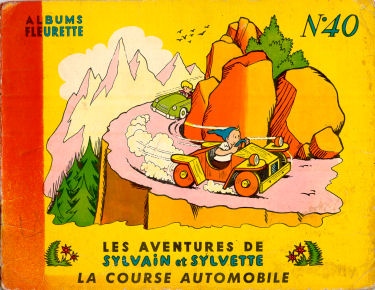
\includegraphics[width=.6\textwidth]{Sylvain+Sylvette_Course.jpg}} 
\newpage           

\item \underline{Résolution du système : }\\

\begin{tabular}{lp{3.5cm}ll}
\multicolumn{4}{l}{
$\begin{cases}
\qquad\dfrac{88}{V_1} -\dfrac{42}{V_2} \!\!\!\!\!\!\!\! &= 1 \\
& \\
\dfrac{106}{V_1} x -\dfrac{24}{V_2} y \!\!\!\!\!\!\!\!&= 1,5  \\
\end{cases}$} \\
& & & \\
\multicolumn{4}{l}{
Le système est linéaire si l'on pose :
       $X=\dfrac{1}{V_1} \text{ et }  Y=\dfrac{1}{V_2}$}\\
& & & \\
\begin{minipage}{4cm}
$\begin{cases}
 \; \; \; 88X - 42Y \!\!\!\!\!\!\!\!&= 1 \\
106X - 24Y\!\!\!\!\!\!\!\! &= 1,5  \\
\end{cases}$ \\
\end{minipage}  &  \multicolumn{1}{|l}{$\begin{array}{l}
                     24\\ -42 \\ 
                  \end{array}$ } & 
                   \begin{minipage}{4cm}       
                         $\begin{cases}
                             \; \; \; 88X - 42Y \!\!\!\!\!\!\!\!&= 1 \\
                            106X - 24Y \!\!\!\!\!\!\!\!&= 1,5  \\
                          \end{cases}$ 
                \end{minipage} &  \multicolumn{1}{|l}{ $\begin{array}{l}
                                        106\\-88\\ 
                                  \end{array}$}\\
& & & \\   
\begin{minipage}{4cm}
$\begin{cases}
 \quad 2112X - 1008Y \!\!\!\!\!\!\!\!&= 24 \\
-4452X - 1008Y \!\!\!\!\!\!\!\!&= -63  \\
\end{cases}$ \\
\end{minipage}  &  & 
                   \begin{minipage}{4cm}       
                         $\begin{cases}
                             \quad 9328X - 4452Y \!\!\!\!\!\!\!\!&= 106 \\
                            -9328X + 2112Y \!\!\!\!\!\!\!\!&= -132  \\
                          \end{cases}$ 
                \end{minipage} &  \\
& & & \\                           
\cline{1-1} \cline{3-3}
\multicolumn{1}{l}{$\qquad \qquad \; \; \; -2340X = -39$} &&
               \multicolumn{1}{l}{$\qquad \qquad \; \; \; -2340Y =-26$}&\\
$\qquad \qquad \qquad \quad \;\; \; X = \dfrac{1}{60}$ && $\qquad \qquad \qquad \quad \;  \; \; Y = \dfrac{1}{90}$& \\
\end{tabular}\\

Il vient : $\dfrac{1}{V_1} = \dfrac{1}{60} $ 
       et  $\dfrac{1}{V_2} = \dfrac{1}{90} $\\


\item \underline{Réponse au problème } :\\

Sylvain roule à 60km/h et les 2 Sylvettes à 90km/h.
  
\end{enumerate} 

\ifdefined\COMPLETE
\else
    \end{document}
\fi  \newpage $\;$ \newpage

\section{Trigonométrie}
\subsection{Cercle trigonométrique}
On appelle cercle trigonométrique tout cercle de rayon $R=1$ sur lequel on a choisi une origine $I$ et un sens de parcours appelé « sens trigonométrique ». 

%------------- Cerlcle trigonométrique ------------------

\hspace*{2cm}
\begin{tikzpicture}[line cap=round,line join=round,>=triangle 45,x=1.0cm,y=1.0cm,scale=.8]
\clip(-3,-3) rectangle (3,3);
\draw [color=gray] (0,0) circle (2cm);
\draw (0,0)-- (2,0);
\draw [shift={(0,0)}] plot[domain=0.17:1.12,variable=\t]({1*2.35*cos(\t r)+0*2.35*sin(\t r)},{0*2.35*cos(\t r)+1*2.35*sin(\t r)});
\draw [->] (1.05,2.1) -- (1.03,2.11);
\fill (0,0) circle (1.5pt);
\draw (0,0) node [below]{$O$};
\fill (2,0) circle (1.5pt);
\draw(2,0) node [right] {$I$};
% \draw (-1/2, sqrt(3)/2) node [left] {$I'$};
\end{tikzpicture}\raisebox{10ex}{$R=OI=1$}
 
\subsection{Image d'un nombre réel sur le cercle trigonométrique}

Soit $\mathcal{C}$ un cercle trigonométrique.

$\mathcal{P} = 2{\pi}R = 2\pi \text{ puisque } R=1$ \\ 

\begin{itemize}
\item [\ding{87}] À tout nombre réel $x$ correspond un point et un seul de $\mathcal{C}$ appelé « image de $x$ sur $\mathcal{C}$ 
noté $M(x)$.\\

$M(\pi) = I'$ 
\item [\ding{87}] Tout point $M$ de  $\mathcal{C}$ est l'image d'une infinité de nombres réels.

\begin{minipage}{9cm}
\begin{tabbing}
Si \= $M$ est $\qquad\quad$ \= l'image de $x$ sur  $\mathcal{C}$\\
   \>  $M$ est aussi \> l'image de $x+2\pi$ \\
   \>  $M$ est aussi \> l'image de $x+4\pi$ \\  
   \>  $M$ est aussi \> l'image de $x+6\pi$\ldots  \\   
   \>  $M$ est aussi \> l'image de $x+2k\pi \quad k\in \mathbb{Z}$ \\    
\end{tabbing}
\hspace*{5cm}
\end{minipage}
%
%------- Enroulement des réels sur le cercle trigo --------
% Pour tracer les courbes de Bésier : 
% ajouter, 
% 1 - dans les préférences de TexMaker, 
%     dans  la ligne  pdflatex 
%     "--shell-escape  -enable-write18 " avant "%.tex"
% 2 - un lien vers gnuplot dans le répertoire  texbin 
%     cd /usr/texbin/
%     sudo ln -s /opt/local/bin/gnuplot ./gnuplot
%
\raisebox{-30ex}{\begin{tikzpicture}[line cap=round,line join=round,>=triangle 45,x=1.0cm,y=1.0cm, scale=.55]
\draw[->,color=black] (0,-7.1) -- (0,11.85);
\foreach \y in {-6,-4,-2,2,4,6,8,10}
\draw[shift={(0,\y)},color=black] (2pt,0pt) -- (-2pt,0pt);
\clip(-4.19,-7.1) rectangle (3.6,11.85);
\draw(-1,0) circle (1cm);
\draw (-2,0)-- (0,0);
\draw [shift={(1.63,-0.1)}] plot[domain=2.04:3.11,variable=\t]({1*3.63*cos(\t r)+0*3.63*sin(\t r)},{0*3.63*cos(\t r)+1*3.63*sin(\t r)});
\draw[smooth,samples=100,domain=0.0:1.0] plot[parametric] function{(1-t)**3*0.01+3*(1-t)**2*t*(-2.81)+3*(1-t)*t**2*(-2.81)+t**3*(-1),(1-t)**3*4.72+3*(1-t)**2*t*2.77+3*(1-t)*t**2*(-1.53)+t**3*(-1)};
\draw[smooth,samples=100,domain=0.0:1.0] plot[parametric] function{(1-t)**3*0+3*(1-t)**2*t*(-7)+3*(1-t)*t**2*2.23+t**3*0,(1-t)**3*6.28+3*(1-t)**2*t*(-2)+3*(1-t)*t**2*(-4.14)+t**3*0};
\draw [shift={(-0.13,-0.64)}] plot[domain=3.54:4.85,variable=\t]({1*0.94*cos(\t r)+0*0.94*sin(\t r)},{0*0.94*cos(\t r)+1*0.94*sin(\t r)});
\draw [shift={(1.64,5.56)}] plot[domain=1.97:2.71,variable=\t]({1*4.2*cos(\t r)+0*4.2*sin(\t r)},{0*4.2*cos(\t r)+1*4.2*sin(\t r)});
\draw [shift={(0.64,7.45)}] plot[domain=1.75:2.8,variable=\t]({1*3.6*cos(\t r)+0*3.6*sin(\t r)},{0*3.6*cos(\t r)+1*3.6*sin(\t r)});
\draw[smooth,samples=100,domain=0.0:1.0] plot[parametric] function{(1-t)**3*0+3*(1-t)**2*t*(-9.62)+3*(1-t)*t**2*7.32+t**3*(-1),(1-t)**3*7.85+3*(1-t)**2*t*(-8.49)+3*(1-t)*t**2*(-1.24)+t**3*1};
\draw [shift={(0.02,0.37)}] plot[domain=1.59:2.59,variable=\t]({1*1.2*cos(\t r)+0*1.2*sin(\t r)},{0*1.2*cos(\t r)+1*1.2*sin(\t r)});
\draw [shift={(-1.27,-0.26)}] plot[domain=4.29:5.13,variable=\t]({1*3.15*cos(\t r)+0*3.15*sin(\t r)},{0*3.15*cos(\t r)+1*3.15*sin(\t r)});
\draw [shift={(-0.52,-0.36)}] plot[domain=4.13:4.83,variable=\t]({1*4.39*cos(\t r)+0*4.39*sin(\t r)},{0*4.39*cos(\t r)+1*4.39*sin(\t r)});
\draw [shift={(0.18,-1.34)}] plot[domain=3.85:4.68,variable=\t]({1*4.95*cos(\t r)+0*4.95*sin(\t r)},{0*4.95*cos(\t r)+1*4.95*sin(\t r)});
\draw (-1,-1) -- (-1,1) ; 
\draw [->] (-2.73,8.71) -- (-2.75,8.66);
\draw [->] (-2.12,7.42) -- (-2.17,7.31);
\draw [->] (-2.4,-3.2) -- (-2.56,-3.14);
\draw [->] (-2.85,-4.07) -- (-2.92,-4.02);
\draw [->] (-3.51,-4.64) -- (-3.57,-4.57);
\draw [->] (.01,-.02) -- (0,0);
\draw [->] (-0.99,1.01) -- (-1,1);
\draw [->] (-0.98,.995) -- (-1,1);
\draw [->] (-0.99,-1.02) -- (-1,-1);
\draw [->] (-1.01,-1) -- (-1,-1);
\draw [->] (-2,.01) -- (-2,0);
\fill  (0,1.57) circle (1.5pt);
\draw (0,1.57) node [right] {${\pi}/2$};
\fill  (0,3.14) circle (1.5pt);
\draw (0,3.14) node [right]{$\pi$};
\fill  (0,9.42) circle (1.5pt);
\draw (0,9.42) node [right]{$3\pi$};
\fill  (0,11) circle (1.5pt);
\draw (0,11) node [right]{$\dfrac{7\pi}{2}$};
\fill  (0,-3.14) circle (1.5pt);
\draw (0,-3.14) node [right]{$-\pi$};
\fill  (0,-4.71) circle (1.5pt);
\draw (0,-4.71) node [right]{$-\dfrac{3\pi}{2}$};
\fill  (0,-1.57) circle (1.5pt);
\draw (0,-1.57) node [right]{$-\dfrac{\pi}{2}$};
\fill  (0,-6.28) circle (1.5pt);
\draw (0,-6.28) node [right]{$-2\pi$};
\fill  (-1,0) circle (1.5pt);
\draw (-1.28,-0.16) node {$O$};
\fill  (0,4.72) circle (1.5pt);
\draw (0,4.72) node [right]{$\dfrac{3\pi}{2}$};
\fill  (-1,-1) circle (1.5pt);
\draw (-1.1,-1) node [below] {$J'$};
\fill  (0,6.28) circle (1.5pt);
\draw (0,6.28) node [right]{$2\pi$};
\fill  (0,0) circle (1.5pt);
\draw (0,0) node [right]{$I$};
\fill  (-2,0) circle (1.5pt);
\draw (-1.7,0.27) node {$I'$};
\fill  (0,7.85) circle (1.5pt);
\draw (0,7.85) node [right]{$\dfrac{5\pi}{2}$};
\fill  (-1,1) circle (1.5pt);
\draw (-0.87,1.28) node {$J$};
\end{tikzpicture}}

\end{itemize}
\newpage

% ---------- Points remarquable du cercle trigo -----------

\begin{tikzpicture}[line cap=round,line join=round,>=triangle 45,x=1.0cm,y=1.0cm, scale=4]
\clip(-1.4,-1.4) rectangle (1.5,1.2);
\draw(0,0) circle (1cm);
\draw [dash pattern=on 1pt off 1pt,color=gray] (-1,1)-- (-1,-1);
\draw [dash pattern=on 1pt off 1pt,color=gray] (-1,-1)-- (1,-1);
\draw [dash pattern=on 1pt off 1pt,color=gray] (1,-1)-- (1,1);
\draw [dash pattern=on 1pt off 1pt,color=gray] (1,1)-- (-1,1);
\draw (-1,1)-- (1,-1);
\draw (1,1)-- (-1,-1);
\draw (0,1) node[above left] {$J$};
\draw [line width=1.2pt] (0,1)-- (0,-1);
\draw [color=violet](1,0) node[above right] {$M(0)$};
\draw [color=violet](1,0) node[below right] {$M(2\pi)\ldots$};
\draw [color=violet](-1,0) node[below left] {$ M(\pi) $};
\draw [dash pattern=on 1pt off 1pt,color=gray] (-0.5,0.87)-- (0.5,0.87);
\draw [dash pattern=on 1pt off 1pt,color=gray] (0.5,0.87)-- (0.5,-0.87);
\draw [dash pattern=on 1pt off 1pt,color=gray] (0.5,-0.87)-- (-0.5,-0.87);
\draw [dash pattern=on 1pt off 1pt,color=gray] (-0.5,-0.87)-- (-0.5,0.87);
\draw [dash pattern=on 1pt off 1pt,color=gray] (-0.87,0.5)-- (0.87,0.5);
\draw [dash pattern=on 1pt off 1pt,color=gray] (0.87,0.5)-- (0.87,-0.5);
\draw [dash pattern=on 1pt off 1pt,color=gray] (0.87,-0.5)-- (-0.87,-0.5);
\draw [dash pattern=on 1pt off 1pt,color=gray] (-0.87,-0.5)-- (-0.87,0.5);
\draw [line width=1.2pt] (-1,0)-- (1,0);
\begin{scriptsize}
\fill  (0,0) circle (.5pt);
\draw (0,0) node [below left]{$O$};
\fill [color=blue] (0.71,0.71) circle (.5pt);
\draw[color=blue] (0.71,0.71) node[right] {$M(\dfrac{\pi}{4})$};
\fill [color=blue] (-0.71,0.71) circle (.5pt);
\draw[color=blue] (-0.71,0.71) node [left]{$M(\dfrac{3\pi}{4})$};
\fill [color=VertClair] (0.87,0.5) circle (.5pt);
\draw[color=VertClair] (0.87,0.5) node [right] {$M(\dfrac{\pi}{6})$};
\fill [color=darkgreen] (0.5,0.87) circle (.5pt);
\draw[color=darkgreen] (0.5,0.87) node [right]{$M(\dfrac{\pi}{3})$};
\fill [color=violet] (0,1) circle (.5pt);
\draw[color=violet] (0,1) node [above right]{$M(\dfrac{\pi}{2})$};
\fill [color=darkgreen] (-0.5,0.87) circle (.5pt);
\draw[color=darkgreen] (-0.5,0.87) node [left]{$M(\dfrac{2\pi}{3)})$};
\fill [color=VertClair] (-0.87,0.5) circle (.5pt);
\draw[color=VertClair] (-0.87,0.5) node [left]{$M(\dfrac{5\pi}{6})$};
\fill [color=blue] (-1,0) circle (.5pt);
\draw[color=blue] (-1,0) node [above left]{$I'$};
\fill [color=blue] (1,0) circle (.5pt);
\draw[color=blue] (1,0) node [above left]{$I$};
\fill [color=blue] (0,-1) circle (.5pt);
\draw[color=blue] (0,-1) node[below left] {$J'$};
\fill [color=VertClair] (-0.87,-0.5) circle (.5pt);
\draw[color=VertClair] (-.87,-0.5) node[left]{$M(\dfrac{7\pi}{6})$};
\fill [color=blue] (-0.71,-0.71) circle (.5pt);
\draw[color=blue] (-0.71,-0.71) node [left]{$M(\dfrac{5\pi}{4})$};
\fill [color=darkgreen] (-0.5,-0.87) circle (.5pt);
\draw[color=darkgreen] (-0.5,-0.87) node [left]{$M(\dfrac{4\pi}{3})$};
\fill [color=violet] (0,-1) circle (.5pt);
\draw[color=violet] (0,-1) node [below right]{$M(\dfrac{3\pi}{2})$};
\fill [color=darkgreen] (0.5,-0.87) circle (.5pt);
\draw[color=darkgreen] (0.5,-0.87) node [right] {$(\dfrac{5\pi}{3})$};
\fill [color=blue] (0.71,-0.71) circle (.5pt);
\draw[color=blue] (0.71,-0.71) node [right] {$M(\dfrac{7\pi}{4})$};
\fill [color=VertClair] (0.87,-0.5) circle (.5pt);
\draw[color=VertClair](0.87,-0.5)node[right]{$M(\dfrac{11\pi}{6})$};
\end{scriptsize}
\end{tikzpicture}\\

Notion de congruence 

$\dfrac{5\pi}{2} \equiv \dfrac{\pi}{2} \left[2\pi\right] \text{ car } \dfrac{5\pi}{2}-\dfrac{\pi}{2} = 2\pi \longleftarrow \text{ Un tour de cercle.}$\\

$\dfrac{9\pi}{2} \equiv \dfrac{\pi}{2} \left[2\pi\right] \text{ car } \dfrac{9\pi}{2}-\dfrac{\pi}{2} = 4\pi \longleftarrow \text{ Deux tours de cercle.}$\\

$\dfrac{15\pi}{2} \cancel{\equiv} \dfrac{\pi}{2} \left[2\pi\right] \text{ car } \dfrac{15\pi}{2}-\dfrac{\pi}{2} = 7\pi \longleftarrow \dfrac{7}{2}\text{ tours de cercle.}$\\

Exercice : Placer sur un cercle trigonométrique les images de : \\
$\dfrac{223\pi}{6},\quad  \dfrac{252\pi}{4}, \quad \dfrac{431\pi}{3},\quad  \dfrac{1035\pi}{4}, \quad \dfrac{1702\pi}{3}, \quad \dfrac{2015\pi}{6}$ \\

\bigskip 

\begin{tabular}{c@{}c@{}c@{}c@{}c@{}l}
\ding{43} 
   $\qquad\dfrac{223\pi}{6}  $ & 
        $ \equiv \dfrac{7\pi}{6}   $ &
           $ \left[2\pi\right] $ & 
               $\text{ car } \dfrac{223\pi}{6}-\dfrac{7\pi}{6}  $ & 
                  $ = 36\pi   $ &
                    $ \longleftarrow \text{ 18 tours de cercle.}$\\
&&&\\
\ding{43}$\qquad\dfrac{291\pi}{4}   $ & $ \equiv \dfrac{3\pi}{4}   $ & $ \left[2\pi\right] $ & $\text{ car } \dfrac{291\pi}{4}-\dfrac{3\pi}{4}  $ & $ = 72\pi   $ & $ \longleftarrow \text{ 36 tours de cercle.}$\\
&&&\\
\ding{43}$\qquad\dfrac{431\pi}{3}   $ & $ \equiv \dfrac{5\pi}{3}   $ & $ \left[2\pi\right] $ & $\text{ car } \dfrac{231\pi}{3}-\dfrac{5\pi}{3}  $ & $ = 142\pi   $ & $ \longleftarrow \text{ 71 tours de cercle.}$\\
&&&\\
\ding{43}$\qquad\dfrac{1035\pi}{4}   $ & $ \equiv \dfrac{3\pi}{4}   $ & $ \left[2\pi\right] $ & $\text{ car } \dfrac{1035\pi}{4}-\dfrac{3\pi}{4}  $ & $ = 258\pi   $ & $ \longleftarrow \text{ 129 tours de cercle.}$\\
&&&\\
\ding{43}$\qquad\dfrac{1702\pi}{3}   $ & $ \equiv \dfrac{4\pi}{3}   $ & $ \left[2\pi\right] $ & $\text{ car } \dfrac{1702\pi}{3}-\dfrac{4\pi}{3}  $ & $ = 566\pi   $ & $ \longleftarrow \text{ 283 tours de cercle.}$\\
&&&\\
\ding{43}$\qquad\dfrac{2015\pi}{6}   $ & $ \equiv \dfrac{11\pi}{6}   $ & $ \left[2\pi\right] $ & $\text{ car } \dfrac{2015\pi}{6}-\dfrac{11\pi}{6}  $ & $ = 334\pi   $ & $ \longleftarrow \text{ 167 tours de cercle.}$\\
\end{tabular}

\newpage

\subsection{Cosinus et sinus d'un nombre réel}

Soit $\mathcal{C}$ un cercle trigonométrique.\\
Soit $M(x)$ l'image de $x$ sur $\mathcal{C}$.\\
Soit $H$ le projeté orthogonal de $M$ sur $(OI)$.\\
Soit $K$ le projeté orthogonal de $M$ sur $(OJ)$.\\

% ------•---- Projetés des points du cercle trigo -----------


\begin{tikzpicture}[line cap=round,line join=round,>=triangle 45,x=1.0cm,y=1.0cm,scale=.8]
\clip(0.3,1) rectangle (14,12.56);
\draw[line width=0.4pt,color=red] (3,11.44) -- (3.21,11.44) -- (3.21,11.65) -- (3,11.65) -- cycle; 
\draw[line width=0.4pt,color=red] (4.13,10.21) -- (3.92,10.21) -- (3.92,10) -- (4.13,10) -- cycle; 
\draw[line width=0.4pt,color=red] (9.79,11) -- (9.79,10.79) -- (10,10.79) -- (10,11) -- cycle; 
\draw[line width=0.4pt,color=red] (8.48,10) -- (8.48,10.21) -- (8.27,10.21) -- (8.27,10) -- cycle; 
\draw[line width=0.4pt,color=red] (1.99,3.79) -- (2.2,3.79) -- (2.2,4) -- (1.99,4) -- cycle; 
\draw[line width=0.4pt,color=red] (3,2.49) -- (2.79,2.49) -- (2.79,2.27) -- (3,2.27) -- cycle; 
\draw[line width=0.4pt,color=red] (11.51,4) -- (11.51,3.79) -- (11.72,3.79) -- (11.72,4) -- cycle; 
\draw[line width=0.4pt,color=red] (10.21,2.98) -- (10.21,3.19) -- (10,3.19) -- (10,2.98) -- cycle; 
\draw(3,4) circle (2cm);
\draw(10,4) circle (2cm);
\draw(3,10) circle (2cm);
\draw(10,10) circle (2cm);
\draw (1,10)-- (5,10);
\draw (3,12)-- (3,8);
\draw [dash pattern=on 5pt off 5pt,color=red] (4.13,11.65)-- (3,11.65);
\draw [dash pattern=on 5pt off 5pt,color=red] (4.13,11.65)-- (4.13,10);
\draw (4.6,8.66) node[anchor=north west] {\parbox{2.12 cm}{${\color{blue}\cos x=OH}\\{\color{Green}\sin x = OK}$}};
\draw [line width=1.6pt,very thick,color=Green] (3,11.65)-- (3,10);
\draw [line width=1.6pt,very thick,color=blue] (3,10)-- (4.13,10);
\draw (10,12)-- (10,8);
\draw [dash pattern=on 5pt off 5pt,color=red] (8.27,10)-- (8.27,11);
\draw (12,10)-- (8,10);
\draw [dash pattern=on 5pt off 5pt,color=red] (8.27,11)-- (10,11);
\draw (10,6)-- (10,2);
\draw (8,4)-- (12,4);
\draw [dash pattern=on 5pt off 5pt,color=red] (11.72,4)-- (11.72,2.98);
\draw [dash pattern=on 5pt off 5pt,color=red] (11.72,2.98)-- (10,2.98);
\draw (1,4)-- (5,4);
\draw (3,6)-- (3,2);
\draw [dash pattern=on 5pt off 5pt,color=red] (3,2.27)-- (1.99,2.27);
\draw [dash pattern=on 5pt off 5pt,color=red] (1.99,2.27)-- (1.99,4);
\draw (0,0.24) node[anchor=north west] {\parbox{2.12 cm}{${\color{blue}\cos x=OH}\\{\color{Green}\sin x = OK}$}};
\draw (11.68,8.68) node[anchor=north west] {\parbox{2.2 cm}{${\color{blue}\cos x=-OH}\\{\color{Green}\sin x = OK}$}};
\draw (4.62,2.7) node[anchor=north west] {\parbox{2.2 cm}{${\color{blue}\cos x= -OH}\\{\color{Green}\sin x = -OK}$}};
\draw (11.62,2.6) node[anchor=north west] {\parbox{2.16 cm}{${\color{blue}\cos x=OH}\\{\color{Green}\sin x = -OK}$}};
\draw [very thick, color=blue] (8.27,10)-- (10,10);
\draw [very thick,color=Green] (10,10)-- (10,11);
\draw [very thick, color=blue] (3,4)-- (1.99,4);
\draw [very thick,color=Green] (3,4)-- (3,2.27);
\draw [very thick, color=blue] (10,4)-- (11.72,4);
\draw [very thick,color=Green] (10,4)-- (10,2.98);

\fill (3,4) circle (1.5pt);
\draw(3,4) node [below left]{$O$};
\fill (10,4) circle (1.5pt);
\draw(10,4) node [below left]{$O$};
\fill (3,10) circle (1.5pt);
\draw(3,10) node [below left]{$O$};
\fill (10,10) circle (1.5pt);
\draw(10,10) node [below left]{$O$};
\fill (1,10) circle (1.5pt);
\draw(1,10) node [left] {$I'$};
\fill (5,10) circle (1.5pt);
\draw(5.32,10.1) node {$I$};
\fill (3,12) circle (1.5pt);
\draw(3,12) node [above]{$J$};
\fill (3,8) circle (1.5pt);
\draw(3,8) node [below] {$J'$};
\fill [color=red] (4.13,11.65) circle (1.5pt);
\draw[color=red] (4.13,11.65) node [right] {$M(x)$};
\fill [color=red] (3,11.65) circle (1.5pt);
\draw[color=red] (3,11.65) node [left] {$K$};
\fill [color=red] (4.13,10) circle (1.5pt);
\draw[color=red] (4.13,10) node [below] {$H$};
\fill [color=red] (8.27,11) circle (1.5pt);
\draw[color=red] (8.27,11) node [left]{$M(x)$};
\fill [color=red] (1.99,2.27) circle (1.5pt);
\draw[color=red] (1.99,2.27) node [left]{$M(x)$};
\fill [color=red] (11.72,2.98) circle (1.5pt);
\draw[color=red] (11.72,2.98) node [right]{$M(x)$};
\fill [color=red] (10,11) circle (1.5pt);
\draw[color=red] (10,11) node [right]{$K$};
\fill [color=red] (8.27,10) circle (1.5pt);
\draw[color=red] (8.27,10) node [below]{$H$};
\fill [color=red] (10,2.98) circle (1.5pt);
\draw[color=red] (10,2.98) node [left]{$K$};
\fill [color=red] (11.72,4) circle (1.5pt);
\draw[color=red] (11.72,4) node [above]{$H$};
\fill [color=red] (3,2.27) circle (1.5pt);
\draw[color=red] (3,2.27) node [right]{$K$};
\fill [color=red] (1.99,4) circle (1.5pt);
\draw[color=red] (1.99,4) node [above]{$H$};
\fill (8,10) circle (1.5pt);
\draw(8,10)  node [left] {$I'$};
\fill (12,10) circle (1.5pt);
\draw(12,10) node [right] {$I$};
\fill (1,4) circle (1.5pt);
\draw(1,4)  node [left] {$I'$};
\fill (5,4) circle (1.5pt);
\draw(5,4) node [right] {$I$};
\fill (8,4) circle (1.5pt);
\draw(8,4)  node [left] {$I'$};
\fill (12,4) circle (1.5pt);
\draw(12,4) node [right] {$I$};
\fill (10,12) circle (1.5pt);
\draw(10,12) node [above] {$J$};
\fill (10,8) circle (1.5pt);
\draw(10,8) node [below] {$J'$};
\fill (10,6) circle (1.5pt);
\draw(10,6)  node [above] {$J$};
\fill (10,2) circle (1.5pt);
\draw(10,2) node [below] {$J'$};
\fill (3,6) circle (1.5pt);
\draw(3,6)  node [above] {$J$};
\fill (3,2) circle (1.5pt);
\draw(3,2) node [below] {$J'$};

\end{tikzpicture}


% ------•---- Les quatres cadrans --------------------------

Quatre quadrants.

\parbox{5cm}{\begin{tikzpicture}[line cap=round,line join=round,>=triangle 45,x=1.0cm,y=1.0cm, scale=.8]
\clip (0.38,7.29) rectangle (6.04,12.92);
\draw (3,10) circle (2cm);
\draw (1,10)-- (5,10);
\draw (3,12)-- (3,8);
\draw (3.75,10.75)    node {\Huge \ding{172}};
\draw (2.25,10.75)       node {\Huge  \ding{173}};
\draw (2.25,9)     node {\Huge  \ding{174}};
\draw (3.75,9)  node {\Huge  \ding{175}};
\fill (3,10) circle (1.5pt);
\draw (3,10) node [below left]{$O$};
\fill (1,10) circle (1.5pt);
\draw (1,10) node [left] {$I'$};
\fill (5,10) circle (1.5pt);
\draw (5,10) node [right] {$I$};
\fill (3,12) circle (1.5pt);
\draw (3,12) node [above]{$J$};
\fill (3,8) circle (1.5pt);
\draw (3,8) node [below]{$J'$};
\end{tikzpicture}}
\parbox{10cm}{
   \ding{172} $\longrightarrow$\raisebox{-1ex}{$ \begin{array}{c}  
\cos (x) > 0 \\ 
\sin (x) >0 \\ 
   \end{array} 
        \qquad$}  
 \ding{173}
        $\longrightarrow$\raisebox{-1ex}{$\begin{array}{c}  
                 \cos (x) < 0 \\ 
                 \sin (x) > 0 \\ 
               \end{array}$}\\
               
               
\ding{174} 
    $\longrightarrow$\raisebox{-1ex}{$ \begin{array}{c}  
\cos (x) < 0 \\ 
\sin (x) < 0 \\ 
   \end{array} 
        \qquad$}  \ding{175}$\longrightarrow$\raisebox{-1ex}{ $\begin{array}{c}  
                 \cos (x) > 0 \\ 
                 \sin (x) < 0 \\ 
               \end{array}$}\\               
} \\
\renewcommand{\arraystretch }{1.75}
En particulier : 
\begin{quote}
{
\begin{tabular}{l@{$\;$}c@{$\qquad$}l@{$\;$}c}
$\bullet$  & $\cos 0 = 1 $ 
         & $\bullet$ & $\cos \dfrac{\pi}{2} = 0 $ \\  
          & $\sin 0 = 0 $ 
         &  & $\sin \dfrac{\pi}{2} = 1 $ \\  
& & & \\
$\bullet$  & $\cos \pi = -1 $ 
         & $\bullet$ & $\cos \dfrac{3\pi}{2} = 0 $ \\  
  & $\sin \pi = 0 $ 
         & & $\sin \dfrac{3\pi}{2} = -1 $ \\                             
\end{tabular}              
}
\end{quote}
\renewcommand{\arraystretch }{1}
\newpage 

Propriétés fondamentales pour $k \in \mathbb{Z}$  

\begin{quote}
\begin{tabular}{l@{$\,$}cc@{$\,$}l}
\ding{81} & Pour tout $x\in \Re$ & $\bullet$ & $-1
                       \leqslant \cos x  \leqslant 1 $ \\
          &          & $\bullet$ & $-1
                       \leqslant \sin x  \leqslant 1 $ \\
 & & & \\ 
 \ding{81} & Pour tout $x\in \Re$ & $\bullet$ 
                     & $ \cos (x+2k\pi) = \cos x $ \\
       &   & $\bullet$ & $ \sin x  (x+2k\pi) = \sin x $ \\
                        & & & \\ 
 \ding{81} & Pour tout $x\in \Re$ & $\bullet$ 
         & $ \cos^2 (x+2k\pi) + \sin^2 (x+2k\pi) = 1 $ \\

\end{tabular}\\

\bigskip

$(O, \overrightarrow{OI},  \overrightarrow{OJ})$ un repère orthonormal.\\

$M(\cos x, \sin x)$ dans $(O, \overrightarrow{OI},  \overrightarrow{OJ})$. \\

\begin{tabular}{r@{\,}l}
$ \cos^2 (x+2k\pi) + \sin^2 x $ &$= OH^2 + OK^2$\\
 &$= OH^2 + HM^2 $\\
 &$= OM^2$\\
 &$= 1 \qquad \qquad \text{ car }\; OM = 1 $\\ 
\end{tabular}\\

{\renewcommand{\arraystretch }{1.75}
\begin{tabular}{ll}
 
\begin{tikzpicture}[line cap=round,line join=round,>=triangle 45,x=1.0cm,y=1.0cm,scale=1]
\clip(-2.25,-2.38) rectangle (2.37,2.39);
\draw[line width=0.4pt] (0,1.32) -- (0.1,1.32) -- (0.1,1.42) -- (0,1.42) -- cycle; 
\draw[line width=0.4pt] (1.41,0.1) -- (1.31,0.1) -- (1.31,0) -- (1.41,0) -- cycle; 
\draw(0,0) circle (2cm);
\draw (-2,0)-- (2,0);
\draw (0,2)-- (0,-2);
\draw [dash pattern=on 2pt off 2pt] (1.41,1.42)-- (0,1.42);
\draw [dash pattern=on 2pt off 2pt] (1.41,1.42)-- (1.41,0);
\draw [line width=1.6pt] (0,1.42)-- (0,0);
\draw [line width=1.6pt] (0,0)-- (1.41,0);
\draw [line width=0.4pt] (0,2)-- (0,0);
\draw [line width=0.4pt] (0,0)-- (2,0);
\draw [line width=0.4pt] (2,0)-- (2,2);
\draw [line width=0.4pt] (2,2)-- (0,2);
\draw (0,0)-- (2,2);

\fill  (0,0) circle (1.5pt);
\draw(0,0) node [below left] {$O$};
\fill (-2,0) circle (1.5pt);
\draw(-2,0) node [left] {$I'$};
\fill (2,0) circle (1.5pt);
\draw(2,0) node [right] {$I$};
\fill (0,2) circle (1.5pt);
\draw(0,2) node [above] {$J$};
\fill (0,-2) circle (1.5pt);
\draw(0,-2) node [below] {$J'$};
\fill (1.41,1.42) circle (1.5pt);
\draw(1.41,1.42) node [above] {$M$};
\fill (0,1.42) circle (1.5pt);
\draw(0,1.42) node [left]{$K$};
\fill (1.41,0) circle (1.5pt);
\draw(1.41,0) node [below] {$H$};

\end{tikzpicture}


         &  \raisebox{27ex}{ \ding{81}}
            \raisebox{16.5ex}{              
         \parbox{.5\textwidth}{ 
        Cosinus et sinus de $\dfrac{\pi}{4}$ \\
        
        $ \begin{array}{r@{\;}l}
                 \cos^2 x + \sin^2 x              &= 1 \\
\cos^2 (\dfrac{\pi}{4}) + \sin^2 (\dfrac{\pi}{4}) &= 1 \\
                             2 sin^2 \dfrac{\pi}{4}      &= 1 \\ 
                         cos^2    \dfrac{\pi}{4} =     sin^2  \dfrac{\pi}{4} &= 
   \dfrac{1}{2} \quad \text { donc }= \dfrac{\sqrt{2}}{2} \text { ou } \cancel {-\dfrac{\sqrt{2}}{2}}\\  
        \end{array}$
         }}\\
\end{tabular}\\
\vspace*{-1cm}
\begin{center}
\fcolorbox{black}  {white}{
\hbox{
$\cos \dfrac{\pi}{4} = \dfrac{\sqrt{2}}{2} \quad \text{ et } \quad \sin \dfrac{\pi}{4} =  \dfrac{\sqrt{2}}{2} $ 
}}
\end{center}

\bigskip 

\begin{tabular}{ll}
 
% \definecolor{uuuuuu}{rgb}{0.27,0.27,0.27}
% \definecolor{qqffqq}{rgb}{0,1,0}
% \definecolor{ffqqqq}{rgb}{1,0,0}
% \definecolor{qqqqff}{rgb}{0,0,1}
\begin{tikzpicture}[line cap=round,line join=round,>=triangle 45,x=1.0cm,y=1.0cm,scale=1]
\clip(-2.25,-2.38) rectangle (2.37,2.39);
\draw[line width=0.4pt] (0,1.64) -- (0.1,1.64) -- (0.1,1.73) -- (0,1.73) -- cycle; 
\draw[line width=0.4pt] (1,0.1) -- (0.9,0.1) -- (0.9,0) -- (1,0) -- cycle; 
\draw(0,0) circle (2cm);
\draw (-2,0)-- (2,0);
\draw (0,2)-- (0,-2);
\draw [dash pattern=on 2pt off 2pt] (1,1.73)-- (0,1.73);
\draw [dash pattern=on 2pt off 2pt] (1,1.73)-- (1,0);
\draw [line width=1.6pt] (0,1.73)-- (0,0);
\draw [line width=1.6pt] (0,0)-- (1,0);
\draw  (0,0)-- (2,0);
\draw  (2,0)-- (1,1.73);
\draw  (1,1.73)-- (0,0);

\fill  (0,0) circle (1.5pt);
\draw(0,0) node [below left] {$O$};
\fill (-2,0) circle (1.5pt);
\draw(-2,0) node [left] {$I'$};
\fill (2,0) circle (1.5pt);
\draw(2,0) node [right] {$I$};
\fill (0,2) circle (1.5pt);
\draw(0,2) node [above] {$J$};
\fill (0,-2) circle (1.5pt);
\draw(0,-2) node [below] {$J'$};
\fill  (1,1.73) circle (1.5pt);
\draw (1.1,1.73) node [right]{$M$};
\fill  (0,1.73) circle (1.5pt);
\draw (0,1.73) node [left] {$K$};
\fill  (1,0) circle (1.5pt);
\draw (1,0) node [below] {$H$};
\end{tikzpicture}

         &  \raisebox{31ex}{ \ding{81}}
            \raisebox{10ex}{              
         \parbox{.5\textwidth}{ 
        Cosinus et sinus de $\dfrac{\pi}{3}$ \\
        
        $ \begin{array}{r@{\;}l}
                 \cos^2 x + \sin^2 x              &= 1 \\
\cos^2 (\dfrac{\pi}{3}) + \sin^2 (\dfrac{\pi}{3}) &= 1 \\
                                       & \qquad \qquad 0H=\dfrac{1}{2} \\
                     \dfrac{1}{4} + \sin^2 (\dfrac{\pi}{3})    &= 1 \\
                       \sin^2 (\dfrac{\pi}{3}) &= 1 - \dfrac{1}{4} \\
                          \sin^2 (\dfrac{\pi}{3}) -\dfrac{3}{4}  &= 0 \\ 
 \left( \sin (\dfrac{\pi}{3} - \sqrt{\dfrac{3}{4}}\right)  \left( \sin (\dfrac{\pi}{3}) +\sqrt{\dfrac{3}{4}}\right) &= 0 \\       
                                   \sin (\dfrac{\pi}{3}) &= 
\dfrac{\sqrt{3}}{2} \text { ou } \cancel {-\dfrac{\sqrt{3}}{2}}\\  
        \end{array}$
         }}\\         
\end{tabular}\\
}
\renewcommand{\arraystretch }{1}
\begin{center}
\fcolorbox{black}  {white}{
\hbox{
$\cos \dfrac{\pi}{3} = \dfrac{1}{2} \quad \text{ et } \quad \sin \dfrac{\pi}{3} =  \dfrac{\sqrt{3}}{2} $ 
}}
\end{center}

\newpage

{\renewcommand{\arraystretch }{1.75}
\begin{tabular}{ll}

\begin{tikzpicture}[line cap=round,line join=round,>=triangle 45,x=1.0cm,y=1.0cm]
\clip(-2.4,-2.38) rectangle (2.8,2.39);
\draw(0,0) circle (2cm);
\draw (-2,0)-- (2,0);
\draw (0,2)-- (0,-2);
\draw [dash pattern=on 2pt off 2pt] (1.73,1)-- (0,1);
\draw [dash pattern=on 2pt off 2pt] (1.73,1)-- (1.73,0);
\draw [line width=1.6pt] (0,1)-- (0,0);
\draw [line width=1.6pt] (0,0)-- (1.73,0);
\draw [line width=2pt](0,0)-- (1.73,1);
\draw [line width=2pt](1.73,1)-- (0,2);
\draw [line width=2pt](0,0)-- (0,2);
\draw (0,2)-- (0,0);
\fill  (0,0) circle (1.5pt);
\draw(0,0) node [below left] {$O$};
\fill (-2,0) circle (1.5pt);
\draw(-2,0) node [left] {$I'$};
\fill (2,0) circle (1.5pt);
\draw(2,0) node [right] {$I$};
\fill (0,2) circle (1.5pt);
\draw(0,2) node [above] {$J$};
\fill (0,-2) circle (1.5pt);
\draw(0,-2) node [below] {$J'$};
\fill  (1.73,1) circle (1.5pt);
\draw (1.73,1) node [right] {$M(\dfrac{\pi}{6})$};
\fill  (0,1) circle (1.5pt);
\draw (0,1) node [left]{$K$};
\fill  (1.73,0) circle (1.5pt);
\draw (1.73,0) node [below] {$H$};
\end{tikzpicture}
         &  \raisebox{31ex}{ \ding{81}}
            \raisebox{10ex}{              
         \parbox{.5\textwidth}{ 
        Cosinus et sinus de $\dfrac{\pi}{6}$ \\
        
        $ \begin{array}{r@{\;}l}
                 \cos^2 x + \sin^2 x              &= 1 \\
\cos^2 (\dfrac{\pi}{6}) + \sin^2 (\dfrac{\pi}{6}) &= 1 \\
                                       & \qquad \qquad OK=\dfrac{1}{2} \\
                      \cos^2 (\dfrac{\pi}{6})  +\dfrac{1}{4}   &= 1 \\
                       \cos^2 (\dfrac{\pi}{6}) &= 1 - \dfrac{1}{4} \\
                          \cos^2 (\dfrac{\pi}{6}) -\dfrac{3}{4}  &= 0 \\ 
 \left( \cos^2 (\dfrac{\pi}{6}) - \sqrt{\dfrac{3}{4}}\right)  \left( \cos^2 (\dfrac{\pi}{6})) +\sqrt{\dfrac{3}{4}}\right) &= 0 \\       
                                   \cos (\dfrac{\pi}{6}) &= 
\dfrac{\sqrt{3}}{2} \text { ou } \cancel {-\dfrac{\sqrt{3}}{2}}\\  
        \end{array}$
         }}\\         
\end{tabular}\\
}
\renewcommand{\arraystretch }{1}
\begin{center}
\fcolorbox{black}  {white}{
\hbox{
$\cos \dfrac{\pi}{6} = \dfrac{\sqrt{3}}{2} \quad \text{ et } \quad \sin \dfrac{\pi}{6} =  \dfrac{1}{2} $ 
}}
\end{center}
\end{quote}

\vspace{2cm}

\underline{Récapitulation} : \\

\bigskip 

\hspace*{2cm}
{\renewcommand{\arraystretch }{2.3}
\begin{tabular}{|c||c|c|c|c|c|}
\hline
$x$ & $0$ & $\dfrac{\pi}{6}$ & $\dfrac{\pi}{4}$ & $\dfrac{\pi}{3}$ & $\dfrac{\pi}{2}$ \\
\hline
\hline
$\cos x$ & $1$ & $\dfrac{\sqrt{3}}{2}$ & $\dfrac{\sqrt{2}}{2}$ & $\dfrac{1}{2}$ & $0$ \\
\hline
$\sin x$ & $0$ & $\dfrac{1}{2}$ & $\dfrac{\sqrt{2}}{2}$ & $\dfrac{\sqrt{3}}{2}$ & $1$ \\
\hline
\end{tabular}
}

\vspace{2cm}


\centerline{
 \renewcommand{\arraystretch }{2.3}
\begin{tabular}{|c||c|c|c|c|c|c|c|c|c|c|c|c|c|c|c|c|}
\hline
$x$ & $0$ & $\dfrac{\pi}{6}$ & $\dfrac{\pi}{4}$ & $\dfrac{\pi}{3}$ & $\dfrac{\pi}{2}$ & $\dfrac{2\pi}{3}$ & $\dfrac{3\pi}{4}$ & $\dfrac{5\pi}{6}$ & $\pi$ & $\dfrac{7\pi}{6}$ & $\dfrac{5\pi}{4}$ & $\dfrac{4\pi}{3}$ & $\dfrac{3\pi}{2}$ & $\dfrac{5\pi}{3}$ & $\dfrac{7\pi}{4}$ & $\dfrac{11\pi}{6}$ \\
\hline
\hline
$\cos x$ & $1$ & $\dfrac{\sqrt{3}}{2}$ & $\dfrac{\sqrt{2}}{2}$ & $\dfrac{1}{2}$ & $0$
         & $-\dfrac{1}{2}$ & $-\dfrac{\sqrt{2}}{2}$ & $- \dfrac{\sqrt{3}}{2}$ & $-1$ 
         & $-\dfrac{\sqrt{3}}{2}$ & $-\dfrac{\sqrt{2}}{2}$ & $-\dfrac{1}{2}$ & $0$ 
         & $\dfrac{1}{2}$ & $\dfrac{\sqrt{2}}{2}$ & $\dfrac{\sqrt{3}}{2}$\\
\hline
$\sin x$ & $0$ &  $\dfrac{1}{2}$ & $\dfrac{\sqrt{2}}{2}$ & $\dfrac{\sqrt{3}}{2}$ & $1$
         & $\dfrac{\sqrt{3}}{2}$ & $\dfrac{\sqrt{2}}{2}$ & $\dfrac{1}{2}$ & $0$
         & $-\dfrac{1}{2}$ & $-\dfrac{\sqrt{2}}{2}$ & $- \dfrac{\sqrt{3}}{2}$ & $-1$ 
         & $-\dfrac{\sqrt{3}}{2}$ & $-\dfrac{\sqrt{2}}{2}$ & $-\dfrac{1}{2}$\\
\hline
\end{tabular}
}



\newpage

\subsection*{Formules de transposition}

\definecolor{uuuuuu}{rgb}{0.27,0.27,0.27}
\begin{tikzpicture}[line cap=round,line join=round,>=triangle 45,x=1.0cm,y=1.0cm,scale=.8]
\clip(-2.52,-2.76) rectangle (16.6,2.76);
\draw[line width=0.4pt,color=red] (0,1.44) -- (0.21,1.44) -- (0.21,1.65) -- (0,1.65) -- cycle; 
\draw[line width=0.4pt,color=red] (1.13,0.21) -- (0.91,0.21) -- (0.91,0) -- (1.13,0) -- cycle; 
\draw[line width=0.4pt,color=red] (0.21,-1.65) -- (0.21,-1.44) -- (0,-1.44) -- (0,-1.65) -- cycle; 
\draw[line width=0.4pt,color=red] (6.98,1.46) -- (7.19,1.46) -- (7.19,1.68) -- (6.98,1.68) -- cycle; 
\draw[line width=0.4pt,color=red] (8.11,0.24) -- (7.89,0.24) -- (7.89,0.03) -- (8.11,0.03) -- cycle; 
\draw[line width=0.4pt,color=red] (14,1.44) -- (14.21,1.44) -- (14.21,1.65) -- (14,1.65) -- cycle; 
\draw[line width=0.4pt,color=red] (15.13,0.21) -- (14.91,0.21) -- (14.91,0) -- (15.13,0) -- cycle; 
\draw[line width=0.4pt,color=red] (6.07,0.03) -- (6.07,0.24) -- (5.85,0.24) -- (5.85,0.03) -- cycle; 
\draw[line width=0.4pt,color=red] (12.87,-0.21) -- (13.09,-0.21) -- (13.09,0) -- (12.87,0) -- cycle; 
\draw[line width=0.4pt,color=red] (14,-1.44) -- (13.79,-1.44) -- (13.79,-1.65) -- (14,-1.65) -- cycle; 
\draw(0,0) circle (2cm);
\draw (-2,0)-- (2,0);
\draw (0,2)-- (0,-2);
\draw [dash pattern=on 5pt off 5pt,color=red] (1.13,1.65)-- (0,1.65);
\draw [dash pattern=on 5pt off 5pt,color=red] (1.13,1.65)-- (1.13,0);
\draw [line width=1.6pt,color=Green] (0,1.65)-- (0,0);
\draw [line width=1.6pt,color=blue] (0,0)-- (1.13,0);
\draw [dash pattern=on 5pt off 5pt,color=red] (1.13,0)-- (1.13,-1.65);
\draw [dash pattern=on 5pt off 5pt,color=red] (1.13,-1.65)-- (0,-1.65);
\draw [line width=1.6pt,color=Green] (0,-1.65)-- (0,0);
\draw(6.98,0.03) circle (2cm);
\draw (4.98,0.03)-- (8.98,0.03);
\draw (6.98,2.03)-- (6.98,-1.97);
\draw [dash pattern=on 5pt off 5pt,color=red] (8.11,1.68)-- (6.98,1.68);
\draw [dash pattern=on 5pt off 5pt,color=red] (8.11,1.68)-- (8.11,0.03);
\draw [line width=1.6pt,color=Green] (6.98,1.68)-- (6.98,0.03);
\draw [line width=1.6pt,color=blue] (6.98,0.03)-- (8.11,0.03);
\draw(14,0) circle (2cm);
\draw (12,0)-- (16,0);
\draw (14,2)-- (14,-2);
\draw [dash pattern=on 5pt off 5pt,color=red] (15.13,1.65)-- (14,1.65);
\draw [dash pattern=on 5pt off 5pt,color=red] (15.13,1.65)-- (15.13,0);
\draw [line width=1.6pt,color=Green] (14,1.65)-- (14,0);
\draw [line width=1.6pt,color=blue] (14,0)-- (15.13,0);
\draw [dash pattern=on 5pt off 5pt,color=red] (5.85,1.68)-- (6.98,1.68);
\draw [dash pattern=on 5pt off 5pt,color=red] (5.85,1.68)-- (5.85,0.03);
\draw [dash pattern=on 5pt off 5pt,color=red] (12.87,-1.65)-- (15.13,1.65);
\draw [dash pattern=on 5pt off 5pt,color=red] (12.87,-1.65)-- (14,-1.65);
\draw [dash pattern=on 5pt off 5pt,color=red] (12.87,-1.65)-- (12.87,0);
\draw [line width=1.6pt,color=Green] (14,0)-- (14,-1.65);
\draw [line width=1.2pt,color=blue] (14,0)-- (12.87,0);
\fill (0,0) circle (1.5pt);
\draw(0,0) node [below left] {$O$};
\fill (-2,0) circle (1.5pt);
\draw(-2,0) node [left] {$I'$};
\fill (2,0) circle (1.5pt);
\draw(2,0) node [right] {$I$};
\fill (0,2) circle (1.5pt);
\draw(0.01,2.47) node {$J$};
\fill (0,-2) circle (1.5pt);
\draw(-0.09,-2.18) node [below] {$J'$};
\fill [color=red] (1.13,1.65) circle (1.5pt);
\draw[color=red] (1.3,1.91) node {$M(x)$};
\fill [color=red] (0,1.65) circle (1.5pt);
\draw[color=red] (0,1.65) node [left]{$K$};
\fill [color=red] (1.13,0) circle (1.5pt);
\draw[color=red] (1.13,0) node [below left]{$H$};
\fill [color=red] (1.13,-1.65) circle (1.5pt);
\draw[color=red] (1.13,-1.65) node [right]{$M'(x)$};
\fill [color=red] (0,-1.65) circle (1.5pt);
\draw[color=red] (0,-1.65) node [left] {$K'$};
\fill (7,0) circle (1.5pt);
\draw(7,0) node [below left]{$O$};
\fill (5,0) circle (1.5pt);
\draw(5,0) node[below left] {$I'$};
\fill (9,0) circle (1.5pt);
\draw(9,0) node [right] {$I$};
\fill (7,2.5) circle (1.5pt);
\draw(7,2.5) node {$J$};
\fill (7,-2) circle (1.5pt);
\draw(7,-2) node [below] {$J'$};
\fill [color=red] (8.11,1.68) circle (1.5pt);
\draw[color=red] (8.11,1.68) node [right]{$M(x)$};
\fill [color=red] (7,1.68) circle (1.5pt);
\draw[color=red] (7,1.68) node [below left] {$K$};
\fill [color=red] (8.11,0) circle (1.5pt);
\draw[color=red] (8.11,0) node [below]{$H$};
\fill (14,0) circle (1.5pt);
\draw(14,0) node [above left]{$O$};
\fill (12,0) circle (1.5pt);
\draw(12,0) node [left]{$I'$};
\fill (16,0) circle (1.5pt);
\draw(16,0) node [right] {$I$};
\fill (14,2) circle (1.5pt);
\draw(14,2) node [above]{$J$};
\fill (14,-2) circle (1.5pt);
\draw(14,-2) node [below]{$J'$};
\fill [color=red] (15.13,1.65) circle (1.5pt);
\draw[color=red] (15.13,1.65) node [right]{$M(x)$};
\fill [color=red] (14,1.65) circle (1.5pt);
\draw[color=red] (14,1.65) node [left]{$K$};
\fill [color=red] (15.13,0) circle (1.5pt);
\draw[color=red] (15,0) node [below]{$H$};
\fill [color=red] (5.85,1.68) circle (1.5pt);
\draw[color=red] (5.85,1.68) node [left]{$M'(x)$};
\fill (5.85,0) circle (1.5pt);
\draw [color=red] (5.85,0) node [below] {$H'$};
\fill [color=red] (12.87,-1.65) circle (1.5pt);
\draw[color=red] (12.87,-1.65) node [below left]{$M'(x)$};
\fill (12.87,0) circle (1.5pt);
\draw [color=red] (12.87,0) node [above]{$H'$};
\fill (14,-1.65) circle (1.5pt);
\draw [color=red](14,-1.65) node [right] {$K'$};
\end{tikzpicture}


\bigskip 

\centerline{
\begin{tabular}{c@{$\,$}l@{\hspace{3cm}}c@{$\,$}l@{\hspace{3cm}}c@{$\,$}l}
% $\bullet$ & $M'(x) \text{ image de } x $ & 
%      $\bullet$ & $M'(\pi - x) \text{ image de } \pi - x $& 
%           $\bullet$ & $M'(\pi + x) \text{ image de } \pi + x $ \\
&$\cos (-x) = \cos (x) $& &$\cos (\pi -x) = -\cos (x)$&&$\cos (\pi+x) = -\cos (x)$\\
&$\sin(-x) = -\sin (x) $& &$\sin (\pi -x) = \sin (x)$&&$\sin (\pi+x) = \sin (x)$\\
\end{tabular}
}

\centerline{
\begin{tikzpicture}[line cap=round,line join=round,>=triangle 45,x=1.0cm,y=1.0cm, scale=.8]
\clip(-2.33,-2.76) rectangle (10.12,2.59);
\draw[line width=0.4pt,color=red] (0,0.81) -- (0.19,0.81) -- (0.19,1) -- (0,1) -- cycle; 
\draw[line width=0.4pt,color=red] (1.73,0.19) -- (1.54,0.19) -- (1.54,0) -- (1.73,0) -- cycle; 
\draw[line width=0.4pt,color=red] (6.98,1.65) -- (7.18,1.65) -- (7.18,1.45) -- (6.98,1.45) -- cycle; 
\draw[line width=0.4pt,color=red] (8.13,0.19) -- (7.94,0.19) -- (7.94,0) -- (8.13,0) -- cycle; 
\draw[line width=0.4pt,color=red] (0.16,0.09) -- (0.07,0.26) -- (-0.09,0.16) -- (0,0) -- cycle; 
\draw[line width=0.4pt,color=red] (-0.19,1.73) -- (-0.19,1.54) -- (0,1.54) -- (0,1.73) -- cycle; 
\draw[line width=0.4pt,color=red] (-0.81,0) -- (-0.81,0.19) -- (-1,0.19) -- (-1,0) -- cycle; 
\draw(0,0) circle (2cm);
\draw (-2,0)-- (2,0);
\draw (0,2)-- (0,-2);
\draw [dash pattern=on 5pt off 5pt,color=red] (1.73,1)-- (0,1);
\draw [dash pattern=on 5pt off 5pt,color=red] (1.73,1)-- (1.73,0);
\draw [line width=1.6pt,color=Green] (0,1)-- (0,0);
\draw [line width=1.6pt,color=blue] (0,0)-- (1.73,0);
\draw(7,0) circle (2cm);
\draw (5,0)-- (9,0);
\draw (6.98,2.03)-- (6.98,-1.97);
\draw [dash pattern=on 5pt off 5pt,color=red] (8.13,1.65)-- (6.98,1.65);
\draw [dash pattern=on 5pt off 5pt,color=red] (8.13,1.65)-- (8.13,0);
\draw [line width=1.6pt,color=Green] (6.98,1.65)-- (7,0);
\draw [line width=1.6pt,color=blue] (7,0)-- (8.13,0);
\draw [dash pattern=on 2pt off 2pt,color=red] (0,0)-- (-1,1.73);
\draw [dash pattern=on 2pt off 2pt,color=red] (0,0)-- (1.73,1);
\draw [dash pattern=on 5pt off 5pt,color=red] (-1,1.73)-- (0,1.73);
\draw [dash pattern=on 5pt off 5pt,color=red] (-1,1.73)-- (-1,0);
\draw [dotted,color=red] (7,0)-- (8.87,0.7);
\draw [dotted,color=red] (7,0)-- (8.13,1.65);
\draw [dash pattern=on 5pt off 5pt,color=red] (8.87,0)-- (8.87,0.7);
\draw [dash pattern=on 5pt off 5pt,color=red] (8.87,0.7)-- (6.98,0.7);
\fill  (0,0) circle (1.5pt);
\draw (0,0) node [below left]{$O$};
\fill  (-2,0) circle (1.5pt);
\draw (-2,0) node [left]{$I'$};
\fill  (2,0) circle (1.5pt);
\draw (2,0) node [right] {$I$};
\fill  (0,2) circle (1.5pt);
\draw (0,2) node [above] {$J$};
\fill  (0,-2) circle (1.5pt);
\draw (0,-2) node [below] {$J'$};
\fill [color=red] (1.73,1) circle (1.5pt);
\draw[color=red] (1.73,1) node [right] {$M(x)$};
\fill [color=red] (0,1) circle (1.5pt);
\draw[color=red] (0,1) node [left] {$K$};
\fill [color=red] (1.73,0) circle (1.5pt);
\draw[color=red] (1.73,0) node [below] {$H$};
\fill  (7,0) circle (1.5pt);
\draw (7,0) node [below left]{$O$};
\fill  (5,0) circle (1.5pt);
\draw (5,0) node [left] {$I'$};
\fill  (9,0) circle (1.5pt);
\draw (9,0) node [right] {$I$};
\fill  (7,2) circle (1.5pt);
\draw (7,2) node [above] {$J$};
\fill  (7,-2) circle (1.5pt);
\draw (7,-2) node [below] {$J'$};
\fill [color=red] (8.13,1.65) circle (1.5pt);
\draw[color=red] (8.13,1.65) node [right]{$M(x)$};
\fill [color=red] (6.98,1.65) circle (1.5pt);
\draw[color=red] (6.98,1.65) node [left] {$K$};
\fill [color=red] (8.13,0) circle (1.5pt);
\draw[color=red] (8.13,0) node [below] {$H$};
\fill [color=red] (-1,1.73) circle (1.5pt);
\draw[color=red] (-1,1.73) node [left] {$M'(x)$};
\fill [color=red] (0,1.73) circle (1.5pt);
\draw[color=red] (0,1.73) node [right] {$K'$};
\fill [color=red] (-1,0) circle (1.5pt);
\draw[color=red] (-1,0) node [below]{$H'$};
\fill [color=red] (8.87,0.7) circle (1.5pt);
\draw[color=red] (8.87,0.7) node [right] {$M'(x)$};
\fill [color=red] (6.98,0.7) circle (1.5pt);
\draw[color=red] (6.98,0.7) node [left] {$K'$};
\fill [color=red] (8.87,0) circle (1.5pt);
\draw[color=red] (8.87,0) node [below] {$H'$};
\end{tikzpicture}
}

\centerline{\renewcommand{\arraystretch }{2}
\begin{tabular}{c@{$\,$}l@{\hspace{2.5cm}}%
                           c@{$\,$}l}
% $\bullet$ & $M'\left( x+\dfrac{\pi}{2} \right) \text{ est l'image ddu réel  } x $ & 
%      $\bullet$ & $M'\left(\dfrac{\pi}{2} - x\right) \text{ image de } x $ \\
           &$\cos \left(x+\dfrac{\pi}{2}\right) = -\sin (x) $& 
               &$\cos \left(\dfrac{\pi}{2} -x\right) = \sin (x)$\\
          &$\sin \left(x+\dfrac{\pi}{2}\right) = \cos (x) $& 
            &$\sin \left(\dfrac{\pi}{2} -x\right) = \cos (x)$\\
\end{tabular}}

\vspace*{.3cm}

Un superbe exercice : 

Soit $x\in \mathbb{R}$, simplifier : 

\begin{enumerate}

\item \raisebox{-2.8ex}{\renewcommand{\arraystretch }{1}
\begin{tabular}{r@{}l}
$A$&$=\cos x +\cos \left(\dfrac{\pi}{2}-x\right) +\cos \left(x +\dfrac{\pi}{2}\right)+\cos (\pi -x) $\\ 
   &$=\cos x + \sin x - \sin x - \cos x $ \\
   & $= 0$ \\
\end{tabular}}

\item \raisebox{-7ex}{\renewcommand{\arraystretch }{1.6}
\begin{tabular}{r@{$\,$}l}
$A'$&$=\cos \left(\dfrac{\pi}{8}\right) +\cos \left(\dfrac{3\pi}{8}\right)+ \cos \left(\dfrac{5\pi}{8}\right) +\cos \left(\dfrac{7\pi}{8}\right)$\\ 
    &$=\cos \left(\dfrac{\pi}{8}\right) +\cos \left(\dfrac{\pi}{2}-\dfrac{\pi}{8}\right)+ \cos \left(\dfrac{\pi}{2}+\dfrac{\pi}{8}\right) +\cos \left(\pi - \dfrac{\pi}{8}\right)$\\ 
   &$=\cos \dfrac{\pi}{8}+ \sin \dfrac{\pi}{8} -  \sin \dfrac{\pi}{8} - \cos \dfrac{\pi}{8}$  \\
   & $=0$ \\
\end{tabular}}

\item \raisebox{-3ex}{\renewcommand{\arraystretch }{1}
\begin{tabular}{r@{$\,$}l}
 $B$ & $=\sin^2 x 
         + \sin^2\left(\dfrac{\pi}{2} - x\right) 
         + \sin^2\left(x +\dfrac{\pi}{2}\right)
         +\sin^2 (\pi - x) $\\ 
   & $=\sin^2 x + \cos^2 x + \cos^2 x + \sin^2 x $  \\
   & $= 1 + 1 = 2 $ \\
\end{tabular}}

\item \raisebox{-4.5ex}{\renewcommand{\arraystretch }{1.6}
\begin{tabular}{r@{$\,$}l}
$B'$&$= \sin^2 \left(\dfrac{\pi}{8}\right) 
      + \sin^2 \left(\dfrac{\pi}{2} - \dfrac{\pi}{8}\right)) 
      + \sin^2 \left(\dfrac{\pi}{2}+\dfrac{\pi}{8}\right)) +  \sin^2 (\pi - \dfrac{\pi}{8}) $\\ 
    &$=\sin^2 \left(\dfrac{\pi}{8}\right) 
       + \cos^2 \left(\dfrac{\pi}{8}\right) 
       + \cos^2 \left(\dfrac{\pi}{8}\right) 
       + \sin^2 \left(\dfrac{\pi}{8}\right) $  \\
   & $= 1 + 1 = 2 $ \\
\end{tabular}}

\end{enumerate}

\samepage

\newpage 

\renewcommand{\arraystretch }{1}

\subsection{Représentations graphiques}

\subsubsection{Représentation graphique de la fonction sinus}

\begin{tabular}{rl}
$\sin\quad : $ & $\mathbb{R} \longrightarrow \mathbb{R} $ \\
               &  $x \longmapsto \sin x $ \\
               & \\
               & $ {\Large \mathcal{D}_{\sin}} = \mathbb{R} $ \\
\end{tabular}\\

% \definecolor{ttzzqq}{rgb}{0.2,0.6,0} % Vert agreable
% \definecolor{qqzzqq}{rgb}{0,0.6,0}   % Vert agreable
% \definecolor{ffefdv}{rgb}{1,0.94,0.84} % AntiqueWhite pour grid
\begin{tikzpicture}[line cap=round,line join=round,>=triangle 45,x=1.0cm,y=1.0cm,scale=.8]

% \draw [color=AntiqueWhite,, xstep=0.1cm,ystep=0.1cm] (-7.1,-1.54) grid (13.29,2.53);


\draw[->,color=black] (-7.1,0) -- (13.29,0);
\foreach \x in {-6,-4,-2,2,4,6,8,10,12}
\draw[shift={(\x,0)},color=black] (0pt,2pt) -- (0pt,-2pt);
\draw[->] (0,-1.54) -- (0,2.53);
\foreach \y in {-1,1,2}
\draw[shift={(0,\y)},color=black] (2pt,0pt) -- (-2pt,0pt);
\clip(-7.1,-1.54) rectangle (13.29,2.53);
\draw[color=Green, smooth,samples=100,domain=-7.097377544417069:13.285348399587015] plot(\x,{sin(((\x))*180/pi)});

% Délimite les périodes 
\draw (-6.28,2)-- (-6.28,-2);
% \draw (0,2.39)-- (0,-2.27);
\draw (12.57,2)-- (12.57,-2);
\draw (6.28,2)-- (6.28,-2);

\draw (0,2) -- node[below, midway] {Période $2\pi$}  (6.28,2);

\begin{tiny}
\draw  (1.05,0)-- ++(-1.0pt,0 pt) -- ++(2.0pt,0 pt) ++(-1.0pt,-1.0pt) -- ++(0 pt,2.0pt);
\draw (pi/3,0) node [below]{$\dfrac{\pi}{3}$};
\draw  (1.57,0)-- ++(-1.0pt,0 pt) -- ++(2.0pt,0 pt) ++(-1.0pt,-1.0pt) -- ++(0 pt,2.0pt);
\draw (pi/2,0 ) node [below] {$\dfrac{\pi}{2}$};
\draw  (3.67,0)-- ++(-1.0pt,0 pt) -- ++(2.0pt,0 pt) ++(-1.0pt,-1.0pt) -- ++(0 pt,2.0pt);
\draw (2*pi/3,0) node [below]{$\dfrac{2\pi}{3}$};
\draw  (4.71,0)-- ++(-1.0pt,0 pt) -- ++(2.0pt,0 pt) ++(-1.0pt,-1.0pt) -- ++(0 pt,2.0pt);
\draw (3*pi/2,0) node [below] {$\dfrac{3\pi}{2}$};
\draw  (5.76,0)-- ++(-1.0pt,0 pt) -- ++(2.0pt,0 pt) ++(-1.0pt,-1.0pt) -- ++(0 pt,2.0pt);
\draw (5*pi/6,0) node [below] {$\dfrac{5\pi}{6}$};
\draw [color=Green] (6.28,0)-- ++(-1.0pt,-1.0pt) -- ++(2.0pt,2.0pt) ++(-2.0pt,0) -- ++(2.0pt,-2.0pt);
\draw  (2.62,0)-- ++(-1.0pt,0 pt) -- ++(2.0pt,0 pt) ++(-1.0pt,-1.0pt) -- ++(0 pt,2.0pt);
\draw (11*pi/6,0) node [above]{$\dfrac{11\pi}{6}$};
\draw (7*pi/6,0) node [above]{$\dfrac{7\pi}{6}$};
\draw  (0.57,0)-- ++(-1.0pt,0 pt) -- ++(2.0pt,0 pt) ++(-1.0pt,-1.0pt) -- ++(0 pt,2.0pt);
\draw (pi/6,0) node [below] {$\dfrac{\pi}{6}$};
\draw (0,0.5) node [left] {$\dfrac{1}{2}$};
\draw  (0,-0.5)-- ++(-1.0pt,0 pt) -- ++(2.0pt,0 pt) ++(-1.0pt,-1.0pt) -- ++(0 pt,2.0pt);
\draw (0,-0.5) node [left]{$-\dfrac{1}{2}$};
\end{tiny}
\begin{scriptsize}
\draw (pi,0) node [above]{$\pi$};
\draw (2*pi,0) node [below right]{$2\pi$};
\draw (0,1) node[right] {$1$};
\draw  (0,-1)-- ++(-1.0pt,0 pt) -- ++(2.0pt,0 pt) ++(-1.0pt,-1.0pt) -- ++(0 pt,2.0pt);
\draw (0,-1) node [left]{$-1$};
\end{scriptsize}
\fill [color=black,shift={(0.1,2)},rotate=90] (0,0) ++(0 pt,2.25pt) -- ++(1.95pt,-3.375pt)--++(-3.9pt,0 pt) -- ++(1.95pt,3.375pt);
\fill [color=black,shift={(6.18,2)},rotate=270] (0,0) ++(0 pt,2.25pt) -- ++(1.95pt,-3.375pt)--++(-3.9pt,0 pt) -- ++(1.95pt,3.375pt);
\draw [color=Green] (0.52,0.5)-- ++(-1.0pt,-1.0pt) -- ++(2.0pt,2.0pt) ++(-2.0pt,0) -- ++(2.0pt,-2.0pt);
\draw [color=Green] (-6.28,0)-- ++(-1.0pt,-1.0pt) -- ++(2.0pt,2.0pt) ++(-2.0pt,0) -- ++(2.0pt,-2.0pt);
\draw [color=Green] (-5.76,0.5)-- ++(-1.0pt,-1.0pt) -- ++(2.0pt,2.0pt) ++(-2.0pt,0) -- ++(2.0pt,-2.0pt);
\draw [color=Green] (-4.71,1)-- ++(-1.0pt,-1.0pt) -- ++(2.0pt,2.0pt) ++(-2.0pt,0) -- ++(2.0pt,-2.0pt);
\draw [color=Green] (-3.67,0.5)-- ++(-1.0pt,-1.0pt) -- ++(2.0pt,2.0pt) ++(-2.0pt,0) -- ++(2.0pt,-2.0pt);
\draw [color=Green] (-2.62,-0.5)-- ++(-1.0pt,-1.0pt) -- ++(2.0pt,2.0pt) ++(-2.0pt,0) -- ++(2.0pt,-2.0pt);
\draw [color=Green] (-3.14,0)-- ++(-1.0pt,-1.0pt) -- ++(2.0pt,2.0pt) ++(-2.0pt,0) -- ++(2.0pt,-2.0pt);
\draw [color=Green] (-1.57,-1)-- ++(-1.0pt,-1.0pt) -- ++(2.0pt,2.0pt) ++(-2.0pt,0) -- ++(2.0pt,-2.0pt);
\draw [color=Green] (-0.52,-0.5)-- ++(-1.0pt,-1.0pt) -- ++(2.0pt,2.0pt) ++(-2.0pt,0) -- ++(2.0pt,-2.0pt);
\draw [color=Green] (1.05,0.87)-- ++(-1.0pt,-1.0pt) -- ++(2.0pt,2.0pt) ++(-2.0pt,0) -- ++(2.0pt,-2.0pt);
\draw [color=Green] (1.57,1)-- ++(-1.0pt,-1.0pt) -- ++(2.0pt,2.0pt) ++(-2.0pt,0) -- ++(2.0pt,-2.0pt);
\draw [color=Green] (2.09,0.87)-- ++(-1.0pt,-1.0pt) -- ++(2.0pt,2.0pt) ++(-2.0pt,0) -- ++(2.0pt,-2.0pt);
\draw [color=Green] (2.62,0.5)-- ++(-1.0pt,-1.0pt) -- ++(2.0pt,2.0pt) ++(-2.0pt,0) -- ++(2.0pt,-2.0pt);
\draw [color=Green] (3.14,0)-- ++(-1.0pt,-1.0pt) -- ++(2.0pt,2.0pt) ++(-2.0pt,0) -- ++(2.0pt,-2.0pt);
\draw [color=Green] (3.67,-0.5)-- ++(-1.0pt,-1.0pt) -- ++(2.0pt,2.0pt) ++(-2.0pt,0) -- ++(2.0pt,-2.0pt);
\draw [color=Green] (4.71,-1)-- ++(-1.0pt,-1.0pt) -- ++(2.0pt,2.0pt) ++(-2.0pt,0) -- ++(2.0pt,-2.0pt);
\draw [color=Green] (5.76,-0.5)-- ++(-1.0pt,-1.0pt) -- ++(2.0pt,2.0pt) ++(-2.0pt,0) -- ++(2.0pt,-2.0pt);
\draw  (0,0.5)-- ++(-1.0pt,0 pt) -- ++(2.0pt,0 pt) ++(-1.0pt,-1.0pt) -- ++(0 pt,2.0pt);

\begin{pgfonlayer}{background}  
% Attention l'ordre de ces lignes est important 
% Ne pas le modifier   
\draw[step=1mm,ultra thin,AntiqueWhite!10](-7,-2)  grid (14,2.6);
\draw[step=5mm,very thin,AntiqueWhite!30] (-7,-2)  grid (14,2.6);
\draw[step=1cm,very thin,AntiqueWhite!50] (-7,-2)  grid (14,2.6);
\draw[step=5cm,thin,AntiqueWhite]         (-7,-2)  grid (14,2.6);

\end{pgfonlayer} 

\end{tikzpicture}

\bigskip 

La fonction sinus est périodique de période $2\pi$. \\

La fonction est dite \underline{sinusoïde}. 


\bigskip 

\subsubsection{Représentation graphique de la fonction cosinus}

\begin{tabular}{rl}
$\cos\quad : $ & $\mathbb{R} \longrightarrow \mathbb{R} $ \\
               &  $x \longmapsto \cos x $ \\
               & \\
               & $ {\Large \mathcal{D}_{\cos}} = \mathbb{R} $ \\
\end{tabular}\\

% \definecolor{ttzzqq}{rgb}{0.2,0.6,0} % Vert agreable
% \definecolor{qqzzqq}{rgb}{0,0.6,0}   % Vert agreable
% \definecolor{ffefdv}{rgb}{1,0.94,0.84} % AntiqueWhite pour grid
\begin{tikzpicture}[line cap=round,line join=round,>=triangle 45,x=1.0cm,y=1.0cm,scale=.8]
% \draw [color=AntiqueWhite,, xstep=0.1cm,ystep=0.1cm] (-7.1,-1.54) grid (13.29,2.53);
\draw[->,color=black] (-7.1,0) -- (13.29,0);
\foreach \x in {-6,-4,-2,2,4,6,8,10,12}
\draw[shift={(\x,0)},color=black] (0pt,2pt) -- (0pt,-2pt);
\draw[->,color=black] (0,-1.54) -- (0,2.53);
\foreach \y in {-1,1,2}
\draw[shift={(0,\y)},color=black] (2pt,0pt) -- (-2pt,0pt);
\clip(-7.1,-1.54) rectangle (13.29,2.53);
\draw[color=Green, smooth,samples=100,domain=-7.097377544417069:13.285348399587015] plot(\x,{cos(((\x))*180/pi)});

% \draw (-6.28,1.5)-- (-6.28,-2);
% \draw (0,2.39)-- (0,-2.27);
% \draw (12.57,1.5)-- (12.57,-2);
% \draw (6.28,2)-- (6.28,-2);


% Délimite les périodes 
\draw (-6.28,2)-- (-6.28,-2);
% \draw (0,2.39)-- (0,-2.27);
\draw (12.57,2)-- (12.57,-2);
\draw (6.28,2)-- (6.28,-2);

\draw (0,2) -- node[below, midway] {Période $2\pi$}  (6.28,2);
% \draw (1.53,1.78) node] {...};
\begin{tiny}
\draw  (1.05,0)-- ++(-1.0pt,0 pt) -- ++(2.0pt,0 pt) ++(-1.0pt,-1.0pt) -- ++(0 pt,2.0pt);
\draw (pi/3,0) node [below]{$\dfrac{\pi}{3}$};
\draw  (1.57,0)-- ++(-1.0pt,0 pt) -- ++(2.0pt,0 pt) ++(-1.0pt,-1.0pt) -- ++(0 pt,2.0pt);
\draw (pi/2,0 ) node [below] {$\dfrac{\pi}{2}$};
\draw  (3.67,0)-- ++(-1.0pt,0 pt) -- ++(2.0pt,0 pt) ++(-1.0pt,-1.0pt) -- ++(0 pt,2.0pt);
\draw (2*pi/3,0) node [below]{$\dfrac{2\pi}{3}$};
\draw  (4.71,0)-- ++(-1.0pt,0 pt) -- ++(2.0pt,0 pt) ++(-1.0pt,-1.0pt) -- ++(0 pt,2.0pt);
\draw (3*pi/2,0) node [below] {$\dfrac{3\pi}{2}$};
\draw  (5.76,0)-- ++(-1.0pt,0 pt) -- ++(2.0pt,0 pt) ++(-1.0pt,-1.0pt) -- ++(0 pt,2.0pt);
\draw (5*pi/6,0) node [below] {$\dfrac{5\pi}{6}$};
\draw [color=Green] (6.28,0)-- ++(-1.0pt,-1.0pt) -- ++(2.0pt,2.0pt) ++(-2.0pt,0) -- ++(2.0pt,-2.0pt);
\draw  (2.62,0)-- ++(-1.0pt,0 pt) -- ++(2.0pt,0 pt) ++(-1.0pt,-1.0pt) -- ++(0 pt,2.0pt);
\draw (11*pi/6,0) node [above]{$\dfrac{11\pi}{6}$};
\draw (7*pi/6,0) node [above]{$\dfrac{7\pi}{6}$};
\draw  (0.57,0)-- ++(-1.0pt,0 pt) -- ++(2.0pt,0 pt) ++(-1.0pt,-1.0pt) -- ++(0 pt,2.0pt);
\draw (pi/6,0) node [below] {$\dfrac{\pi}{6}$};
\draw (0,0.5) node [left] {$\dfrac{1}{2}$};
\draw  (0,-0.5)-- ++(-1.0pt,0 pt) -- ++(2.0pt,0 pt) ++(-1.0pt,-1.0pt) -- ++(0 pt,2.0pt);
\draw (0,-0.5) node [left]{$-\dfrac{1}{2}$};
\end{tiny}
\begin{scriptsize}
\draw (pi,0) node [above]{$\pi$};
\draw (2*pi,0) node [below right]{$2\pi$};
\draw (0,1) node[right] {$1$};
\draw  (0,-1)-- ++(-1.0pt,0 pt) -- ++(2.0pt,0 pt) ++(-1.0pt,-1.0pt) -- ++(0 pt,2.0pt);
\draw (0,-1) node [left]{$-1$};
\end{scriptsize}
\fill [color=black,shift={(0.1,2)},rotate=90] (0,0) ++(0 pt,2.25pt) -- ++(1.95pt,-3.375pt)--++(-3.9pt,0 pt) -- ++(1.95pt,3.375pt);
\fill [color=black,shift={(6.18,2)},rotate=270] (0,0) ++(0 pt,2.25pt) -- ++(1.95pt,-3.375pt)--++(-3.9pt,0 pt) -- ++(1.95pt,3.375pt);


\draw [color=Green] (0.52-pi/2,0.5)-- ++(-1.0pt,-1.0pt) -- ++(2.0pt,2.0pt) ++(-2.0pt,0) -- ++(2.0pt,-2.0pt);
\draw [color=Green] (-6.28-pi/2,0)-- ++(-1.0pt,-1.0pt) -- ++(2.0pt,2.0pt) ++(-2.0pt,0) -- ++(2.0pt,-2.0pt);
\draw [color=Green] (-5.76-pi/2,0.5)-- ++(-1.0pt,-1.0pt) -- ++(2.0pt,2.0pt) ++(-2.0pt,0) -- ++(2.0pt,-2.0pt);
\draw [color=Green] (-4.71-pi/2,1)-- ++(-1.0pt,-1.0pt) -- ++(2.0pt,2.0pt) ++(-2.0pt,0) -- ++(2.0pt,-2.0pt);
\draw [color=Green] (-3.67-pi/2,0.5)-- ++(-1.0pt,-1.0pt) -- ++(2.0pt,2.0pt) ++(-2.0pt,0) -- ++(2.0pt,-2.0pt);
\draw [color=Green] (-2.62-pi/2,-0.5)-- ++(-1.0pt,-1.0pt) -- ++(2.0pt,2.0pt) ++(-2.0pt,0) -- ++(2.0pt,-2.0pt);
\draw [color=Green] (-3.14-pi/2,0)-- ++(-1.0pt,-1.0pt) -- ++(2.0pt,2.0pt) ++(-2.0pt,0) -- ++(2.0pt,-2.0pt);
\draw [color=Green] (-1.57-pi/2,-1)-- ++(-1.0pt,-1.0pt) -- ++(2.0pt,2.0pt) ++(-2.0pt,0) -- ++(2.0pt,-2.0pt);
\draw [color=Green] (-0.52-pi/2,-0.5)-- ++(-1.0pt,-1.0pt) -- ++(2.0pt,2.0pt) ++(-2.0pt,0) -- ++(2.0pt,-2.0pt);
\draw [color=Green] (1.05-pi/2,0.87)-- ++(-1.0pt,-1.0pt) -- ++(2.0pt,2.0pt) ++(-2.0pt,0) -- ++(2.0pt,-2.0pt);
\draw [color=Green] (1.57-pi/2,1)-- ++(-1.0pt,-1.0pt) -- ++(2.0pt,2.0pt) ++(-2.0pt,0) -- ++(2.0pt,-2.0pt);
\draw [color=Green] (2.09-pi/2,0.87)-- ++(-1.0pt,-1.0pt) -- ++(2.0pt,2.0pt) ++(-2.0pt,0) -- ++(2.0pt,-2.0pt);
\draw [color=Green] (2.62-pi/2,0.5)-- ++(-1.0pt,-1.0pt) -- ++(2.0pt,2.0pt) ++(-2.0pt,0) -- ++(2.0pt,-2.0pt);
\draw [color=Green] (3.14-pi/2,0)-- ++(-1.0pt,-1.0pt) -- ++(2.0pt,2.0pt) ++(-2.0pt,0) -- ++(2.0pt,-2.0pt);
\draw [color=Green] (3.67-pi/2,-0.5)-- ++(-1.0pt,-1.0pt) -- ++(2.0pt,2.0pt) ++(-2.0pt,0) -- ++(2.0pt,-2.0pt);
\draw [color=Green] (4.71-pi/2,-1)-- ++(-1.0pt,-1.0pt) -- ++(2.0pt,2.0pt) ++(-2.0pt,0) -- ++(2.0pt,-2.0pt);
\draw [color=Green] (5.76-pi/2,-0.5)-- ++(-1.0pt,-1.0pt) -- ++(2.0pt,2.0pt) ++(-2.0pt,0) -- ++(2.0pt,-2.0pt);
\draw  (0,0.5)-- ++(-1.0pt,0 pt) -- ++(2.0pt,0 pt) ++(-1.0pt,-1.0pt) -- ++(0 pt,2.0pt);

\begin{pgfonlayer}{background}  
% Attention l'ordre de ces lignes est important 
% Ne pas le modifier   
\draw[step=1mm,ultra thin,AntiqueWhite!10](-7,-2)  grid (14,2.6);
\draw[step=5mm,very thin,AntiqueWhite!30] (-7,-2)  grid (14,2.6);
\draw[step=1cm,very thin,AntiqueWhite!50] (-7,-2)  grid (14,2.6);
\draw[step=5cm,thin,AntiqueWhite]         (-7,-2)  grid (14,2.6);

\end{pgfonlayer} 

\end{tikzpicture}

\bigskip 

La fonction cosinus est périodique de période $2\pi$. \\

La fonction est dite \underline{sinusoïde}. 

\newpage 

\subsubsection{Comparaison des représentations graphiques des fonctions sinus et cosinus}

\centerline{\begin{tabular}{r@{\hspace*{3cm}}l}
    \begin{tabular}{rl}
    \multicolumn{2}{c}{\textcolor{Green} {Cosinus tracé en vert}} \\
    $\cos\quad : $ & $\mathbb{R} \longrightarrow \mathbb{R} $ \\
                   &  $x \longmapsto \cos x $ \\
                   & \\
                   & $ {\Large \mathcal{D}_{\cos}} = \mathbb{R} $ \\
    \end{tabular} & 
                   \begin{tabular}{rl}
                       \multicolumn{2}{c}{\textcolor{Red} {Sinus tracé en rouge}} \\
                    $\sin\quad : $ & $\mathbb{R} \longrightarrow \mathbb{R} $ \\
                                &  $x \longmapsto \sin x $ \\
                                & \\
                                & $ {\Large \mathcal{D}_{\cos}} = \mathbb{R} $ \\
                     \end{tabular}\\
\end{tabular}}

\bigskip 


% \definecolor{ttzzqq}{rgb}{0.2,0.6,0} % Vert agreable
% \definecolor{qqzzqq}{rgb}{0,0.6,0}   % Vert agreable
% \definecolor{ffefdv}{rgb}{1,0.94,0.84} % AntiqueWhite pour grid
\begin{tikzpicture}[line cap=round,line join=round,>=triangle 45,x=1.0cm,y=1.0cm,scale=.8]
% \draw [color=AntiqueWhite,, xstep=0.1cm,ystep=0.1cm] (-7.1,-1.54) grid (13.29,2.53);
\draw[->,color=black] (-7.1,0) -- (13.29,0);
\foreach \x in {-6,-4,-2,2,4,6,8,10,12}
\draw[shift={(\x,0)},color=black] (0pt,2pt) -- (0pt,-2pt);
\draw[->,color=black] (0,-1.54) -- (0,2.53);
\foreach \y in {-1,1,2}
\draw[shift={(0,\y)},color=black] (2pt,0pt) -- (-2pt,0pt);
\clip(-7.1,-1.54) rectangle (13.29,2.53);
\draw[color=Green, smooth,samples=100,domain=-7.097377544417069:13.285348399587015] plot(\x,{cos(((\x))*180/pi)});
\draw[color=red, smooth,samples=100,domain=-7.097377544417069:13.285348399587015] plot(\x,{sin(((\x))*180/pi)});

% \draw (-6.28,1.5)-- (-6.28,-2);
% \draw (0,2.39)-- (0,-2.27);
% \draw (12.57,1.5)-- (12.57,-2);
% \draw (6.28,2)-- (6.28,-2);


% Délimite les périodes 
\draw (-6.28,2)-- (-6.28,-2);
% \draw (0,2.39)-- (0,-2.27);
\draw (12.57,2)-- (12.57,-2);
\draw (6.28,2)-- (6.28,-2);

\draw (0,2) -- node[below, midway] {Période $2\pi$}  (6.28,2);

\begin{tiny}
% \draw  (1.05,0)-- ++(-1.0pt,0 pt) -- ++(2.0pt,0 pt) ++(-1.0pt,-1.0pt) -- ++(0 pt,2.0pt);
%\draw (pi/3,0) node [below]{$\dfrac{\pi}{3}$};
%\draw  (1.57,0)-- ++(-1.0pt,0 pt) -- ++(2.0pt,0 pt) ++(-1.0pt,-1.0pt) -- ++(0 pt,2.0pt);
%\draw (pi/2,0 ) node [below] {$\dfrac{\pi}{2}$};
%\draw  (3.67,0)-- ++(-1.0pt,0 pt) -- ++(2.0pt,0 pt) ++(-1.0pt,-1.0pt) -- ++(0 pt,2.0pt);
%\draw (2*pi/3,0) node [below]{$\dfrac{2\pi}{3}$};
%\draw  (4.71,0)-- ++(-1.0pt,0 pt) -- ++(2.0pt,0 pt) ++(-1.0pt,-1.0pt) -- ++(0 pt,2.0pt);
%\draw (3*pi/2,0) node [below] {$\dfrac{3\pi}{2}$};
%\draw  (5.76,0)-- ++(-1.0pt,0 pt) -- ++(2.0pt,0 pt) ++(-1.0pt,-1.0pt) -- ++(0 pt,2.0pt);
%\draw (5*pi/6,0) node [below] {$\dfrac{5\pi}{6}$};
%\draw [color=Green] (6.28,0)-- ++(-1.0pt,-1.0pt) -- ++(2.0pt,2.0pt) ++(-2.0pt,0) -- ++(2.0pt,-2.0pt);
%\draw  (2.62,0)-- ++(-1.0pt,0 pt) -- ++(2.0pt,0 pt) ++(-1.0pt,-1.0pt) -- ++(0 pt,2.0pt);
%\draw (11*pi/6,0) node [above]{$\dfrac{11\pi}{6}$};
%\draw (7*pi/6,0) node [above]{$\dfrac{7\pi}{6}$};
%\draw  (0.57,0)-- ++(-1.0pt,0 pt) -- ++(2.0pt,0 pt) ++(-1.0pt,-1.0pt) -- ++(0 pt,2.0pt);
%\draw (pi/6,0) node [below] {$\dfrac{\pi}{6}$};

\draw (0,0.5) node [left] {$\dfrac{1}{2}$};
\draw  (0,-0.5)-- ++(-1.0pt,0 pt) -- ++(2.0pt,0 pt) ++(-1.0pt,-1.0pt) -- ++(0 pt,2.0pt);
\draw (0,-0.5) node [left]{$-\dfrac{1}{2}$};
\end{tiny}
\begin{scriptsize}
\draw (pi,0) node [above]{$\pi$};
\draw (2*pi,0) node [below right]{$2\pi$};
\draw (0,1) node[right] {$1$};
\draw  (0,-1)-- ++(-1.0pt,0 pt) -- ++(2.0pt,0 pt) ++(-1.0pt,-1.0pt) -- ++(0 pt,2.0pt);
\draw (0,-1) node [left]{$-1$};
\end{scriptsize}
\fill [color=black,shift={(0.1,2)},rotate=90] (0,0) ++(0 pt,2.25pt) -- ++(1.95pt,-3.375pt)--++(-3.9pt,0 pt) -- ++(1.95pt,3.375pt);
\fill [color=black,shift={(6.18,2)},rotate=270] (0,0) ++(0 pt,2.25pt) -- ++(1.95pt,-3.375pt)--++(-3.9pt,0 pt) -- ++(1.95pt,3.375pt);


\draw [color=Green] (0.52-pi/2,0.5)-- ++(-1.0pt,-1.0pt) -- ++(2.0pt,2.0pt) ++(-2.0pt,0) -- ++(2.0pt,-2.0pt);


\begin{pgfonlayer}{background}  
% Attention l'ordre de ces lignes est important 
% Ne pas le modifier   
\draw[step=1mm,ultra thin,AntiqueWhite!10](-7,-2)  grid (14,2.6);
\draw[step=5mm,very thin,AntiqueWhite!30] (-7,-2)  grid (14,2.6);
\draw[step=1cm,very thin,AntiqueWhite!50] (-7,-2)  grid (14,2.6);
\draw[step=5cm,thin,AntiqueWhite]         (-7,-2)  grid (14,2.6);

\end{pgfonlayer} 

% \clip(-7.1,-1.54) rectangle (13.29,2.53);
% \draw [color=AntiqueWhite,, xstep=0.1cm,ystep=0.1cm] (-7.1,-1.54) grid (13.29,2.53);
%\draw [color=Green] (-6.28-pi/2,0)-- ++(-1.0pt,-1.0pt) -- ++(2.0pt,2.0pt) ++(-2.0pt,0) -- ++(2.0pt,-2.0pt);
%\draw [color=Green] (-5.76-pi/2,0.5)-- ++(-1.0pt,-1.0pt) -- ++(2.0pt,2.0pt) ++(-2.0pt,0) -- ++(2.0pt,-2.0pt);
%\draw [color=Green] (-4.71-pi/2,1)-- ++(-1.0pt,-1.0pt) -- ++(2.0pt,2.0pt) ++(-2.0pt,0) -- ++(2.0pt,-2.0pt);
%\draw [color=Green] (-3.67-pi/2,0.5)-- ++(-1.0pt,-1.0pt) -- ++(2.0pt,2.0pt) ++(-2.0pt,0) -- ++(2.0pt,-2.0pt);
%\draw [color=Green] (-2.62-pi/2,-0.5)-- ++(-1.0pt,-1.0pt) -- ++(2.0pt,2.0pt) ++(-2.0pt,0) -- ++(2.0pt,-2.0pt);
%\draw [color=Green] (-3.14-pi/2,0)-- ++(-1.0pt,-1.0pt) -- ++(2.0pt,2.0pt) ++(-2.0pt,0) -- ++(2.0pt,-2.0pt);
%\draw [color=Green] (-1.57-pi/2,-1)-- ++(-1.0pt,-1.0pt) -- ++(2.0pt,2.0pt) ++(-2.0pt,0) -- ++(2.0pt,-2.0pt);
%\draw [color=Green] (-0.52-pi/2,-0.5)-- ++(-1.0pt,-1.0pt) -- ++(2.0pt,2.0pt) ++(-2.0pt,0) -- ++(2.0pt,-2.0pt);
%\draw [color=Green] (1.05-pi/2,0.87)-- ++(-1.0pt,-1.0pt) -- ++(2.0pt,2.0pt) ++(-2.0pt,0) -- ++(2.0pt,-2.0pt);
%\draw [color=Green] (1.57-pi/2,1)-- ++(-1.0pt,-1.0pt) -- ++(2.0pt,2.0pt) ++(-2.0pt,0) -- ++(2.0pt,-2.0pt);
%\draw [color=Green] (2.09-pi/2,0.87)-- ++(-1.0pt,-1.0pt) -- ++(2.0pt,2.0pt) ++(-2.0pt,0) -- ++(2.0pt,-2.0pt);
%\draw [color=Green] (2.62-pi/2,0.5)-- ++(-1.0pt,-1.0pt) -- ++(2.0pt,2.0pt) ++(-2.0pt,0) -- ++(2.0pt,-2.0pt);
%\draw [color=Green] (3.14-pi/2,0)-- ++(-1.0pt,-1.0pt) -- ++(2.0pt,2.0pt) ++(-2.0pt,0) -- ++(2.0pt,-2.0pt);
%\draw [color=Green] (3.67-pi/2,-0.5)-- ++(-1.0pt,-1.0pt) -- ++(2.0pt,2.0pt) ++(-2.0pt,0) -- ++(2.0pt,-2.0pt);
%\draw [color=Green] (4.71-pi/2,-1)-- ++(-1.0pt,-1.0pt) -- ++(2.0pt,2.0pt) ++(-2.0pt,0) -- ++(2.0pt,-2.0pt);
%\draw [color=Green] (5.76-pi/2,-0.5)-- ++(-1.0pt,-1.0pt) -- ++(2.0pt,2.0pt) ++(-2.0pt,0) -- ++(2.0pt,-2.0pt);
%\draw  (0,0.5)-- ++(-1.0pt,0 pt) -- ++(2.0pt,0 pt) ++(-1.0pt,-1.0pt) -- ++(0 pt,2.0pt);
\end{tikzpicture}

\bigskip 

La représentation graphique de la fonction cosinus est obtenue par translation de la fonction sinus avec un décalage de $\dfrac{\pi}{2}$. \\

En effet, pour tout $x \in \mathbb{R}$ \\
\begin{quote}
$\cos \left(\dfrac{\pi}{2}-x\right) = \sin x$ \\

\smallskip 
$\sin \left(\dfrac{\pi}{2}-x\right) = \cos x$ \\
\end{quote}

\newpage

\subsubsection{Exercice}

\begin{tabular}{r@{\hspace*{3cm}}l}
    \begin{tabular}{rl}
    \multicolumn{2}{c}{\textcolor{Green} {$f$ tracé en vert}} \\
    $f \quad : $ & $\mathbb{R} \longrightarrow \mathbb{R} $ \\
                   &  $x \longmapsto f(x) = \cos x $ \\
                   & $f$ est périodique de période $2\pi$ \\ 
                   & \\
                   & $ {\Large \mathcal{D}_{f}} = \mathbb{R} $ \\
    \end{tabular} & 
                   \begin{tabular}{rl}
                     \multicolumn{2}{c}{\textcolor{Red} {$g$ tracé en rouge}} \\
                    $g \quad : $ & $\mathbb{R} \longrightarrow \mathbb{R} $ \\
                        &  $x \longmapsto \sin \left(\dfrac{1}{2} x\right) $ \\
                                & $g$ est périodique de période $\pi$ \\ 
                                & \\
                                & $ {\Large \mathcal{D}_{g}} = \mathbb{R} $ \\
                     \end{tabular}\\
\end{tabular}

% \definecolor{ttzzqq}{rgb}{0.2,0.6,0} % Vert agreable
% \definecolor{qqzzqq}{rgb}{0,0.6,0}   % Vert agreable
% \definecolor{ffefdv}{rgb}{1,0.94,0.84} % AntiqueWhite pour grid
\begin{tikzpicture}[line cap=round,line join=round,>=triangle 45,x=1.0cm,y=1.0cm,scale=.8]
% \draw [color=AntiqueWhite,, xstep=0.1cm,ystep=0.1cm] (-7.1,-1.54) grid (13.29,2.53);
\draw[->,color=black] (-7.1,0) -- (13.29,0);
\foreach \x in {-6,-4,-2,2,4,6,8,10,12}
\draw[shift={(\x,0)},color=black] (0pt,2pt) -- (0pt,-2pt);
\draw[->,color=black] (0,-1.54) -- (0,2.53);
\foreach \y in {-1,1,2}
\draw[shift={(0,\y)}] (2pt,0pt) -- (-2pt,0pt);
\clip(-7.1,-1.54) rectangle (13.29,2.80);
\draw[color=Green, smooth,samples=100,domain=-7.097377544417069:13.285348399587015] plot(\x,{cos(((\x))*180/pi)});
\draw[color=red, smooth,samples=100,domain=-7.097377544417069:13.285348399587015] plot(\x,{sin(((\x/2))*180/pi)});

% Délimite les périodes 
\draw (-6.28,2)-- (-6.28,-2);
% \draw (0,2.39)-- (0,-2.27);
\draw (12.57,2)-- (12.57,-2);
\draw (6.28,2)-- (6.28,-2);

\draw (0,2) -- node[above, midway] {La période de $f \text{ est } 2\pi$}  (6.28,2);
\draw [<->] (-2*pi,1.5) -- node[below, midway] {La période de $g \text{ est } 4\pi$}  (6.28,1.5);

\begin{tiny}
% \draw  (1.05,0)-- ++(-1.0pt,0 pt) -- ++(2.0pt,0 pt) ++(-1.0pt,-1.0pt) -- ++(0 pt,2.0pt);
% \draw (pi/3,0) node [below]{$\dfrac{\pi}{3}$};
% \draw  (1.57,0)-- ++(-1.0pt,0 pt) -- ++(2.0pt,0 pt) ++(-1.0pt,-1.0pt) -- ++(0 pt,2.0pt);
% \draw (pi/2,0 ) node [below] {$\dfrac{\pi}{2}$};
% \draw  (3.67,0)-- ++(-1.0pt,0 pt) -- ++(2.0pt,0 pt) ++(-1.0pt,-1.0pt) -- ++(0 % pt,2.0pt);
% \draw (2*pi/3,0) node [below]{$\dfrac{2\pi}{3}$};
% \draw  (4.71,0)-- ++(-1.0pt,0 pt) -- ++(2.0pt,0 pt) ++(-1.0pt,-1.0pt) -- ++(0 pt,2.0pt);
% \draw (3*pi/2,0) node [below] {$\dfrac{3\pi}{2}$};
% \draw  (5.76,0)-- ++(-1.0pt,0 pt) -- ++(2.0pt,0 pt) ++(-1.0pt,-1.0pt) -- ++(0 pt,2.0pt);
% \draw (5*pi/6,0) node [below] {$\dfrac{5\pi}{6}$};
% \draw [color=Green] (6.28,0)-- ++(-1.0pt,-1.0pt) -- ++(2.0pt,2.0pt) ++(-2.0pt,0) -- ++(2.0pt,-2.0pt);
% \draw  (2.62,0)-- ++(-1.0pt,0 pt) -- ++(2.0pt,0 pt) ++(-1.0pt,-1.0pt) -- ++(0 pt,2.0pt);
% \draw (11*pi/6,0) node [above]{$\dfrac{11\pi}{6}$};
% \draw (7*pi/6,0) node [above]{$\dfrac{7\pi}{6}$};
% \draw  (0.57,0)-- ++(-1.0pt,0 pt) -- ++(2.0pt,0 pt) ++(-1.0pt,-1.0pt) -- ++(0 pt,2.0pt);
% \draw (pi/6,0) node [below] {$\dfrac{\pi}{6}$};

\draw (0,0.5) node [left] {$\dfrac{1}{2}$};
\draw  (0,-0.5)-- ++(-1.0pt,0 pt) -- ++(2.0pt,0 pt) ++(-1.0pt,-1.0pt) -- ++(0 pt,2.0pt);
\draw (0,-0.5) node [left]{$-\dfrac{1}{2}$};
\end{tiny}
\begin{scriptsize}
\draw (pi,0) node [above]{$\pi$};
\draw (2*pi,0) node [below right]{$2\pi$};
\draw (0,1) node[right] {$1$};
\draw  (0,-1)-- ++(-1.0pt,0 pt) -- ++(2.0pt,0 pt) ++(-1.0pt,-1.0pt) -- ++(0 pt,2.0pt);
\draw (0,-1) node [left]{$-1$};
\end{scriptsize}

\fill [color=black,shift={(0.1,2)},rotate=90] (0,0) ++(0 pt,2.25pt) -- ++(1.95pt,-3.375pt)--++(-3.9pt,0 pt) -- ++(1.95pt,3.375pt);
\fill [color=black,shift={(6.18,2)},rotate=270] (0,0) ++(0 pt,2.25pt) -- ++(1.95pt,-3.375pt)--++(-3.9pt,0 pt) -- ++(1.95pt,3.375pt);


\draw [color=Green] (0.52-pi/2,0.5)-- ++(-1.0pt,-1.0pt) -- ++(2.0pt,2.0pt) ++(-2.0pt,0) -- ++(2.0pt,-2.0pt);
\begin{pgfonlayer}{background}  
% Attention l'ordre de ces lignes est important 
% Ne pas le modifier   
\draw[step=1mm,ultra thin,AntiqueWhite!10](-7,-2)  grid (14,2.6);
\draw[step=5mm,very thin,AntiqueWhite!30] (-7,-2)  grid (14,2.6);
\draw[step=1cm,very thin,AntiqueWhite!50] (-7,-2)  grid (14,2.6);
\draw[step=5cm,thin,AntiqueWhite]         (-7,-2)  grid (14,2.6);

\end{pgfonlayer} 

%\draw [color=Green] (-6.28-pi/2,0)-- ++(-1.0pt,-1.0pt) -- ++(2.0pt,2.0pt) ++(-2.0pt,0) -- ++(2.0pt,-2.0pt);
%\draw [color=Green] (-5.76-pi/2,0.5)-- ++(-1.0pt,-1.0pt) -- ++(2.0pt,2.0pt) ++(-2.0pt,0) -- ++(2.0pt,-2.0pt);
%\draw [color=Green] (-4.71-pi/2,1)-- ++(-1.0pt,-1.0pt) -- ++(2.0pt,2.0pt) ++(-2.0pt,0) -- ++(2.0pt,-2.0pt);
%\draw [color=Green] (-3.67-pi/2,0.5)-- ++(-1.0pt,-1.0pt) -- ++(2.0pt,2.0pt) ++(-2.0pt,0) -- ++(2.0pt,-2.0pt);
%\draw [color=Green] (-2.62-pi/2,-0.5)-- ++(-1.0pt,-1.0pt) -- ++(2.0pt,2.0pt) ++(-2.0pt,0) -- ++(2.0pt,-2.0pt);
%\draw [color=Green] (-3.14-pi/2,0)-- ++(-1.0pt,-1.0pt) -- ++(2.0pt,2.0pt) ++(-2.0pt,0) -- ++(2.0pt,-2.0pt);
%\draw [color=Green] (-1.57-pi/2,-1)-- ++(-1.0pt,-1.0pt) -- ++(2.0pt,2.0pt) ++(-2.0pt,0) -- ++(2.0pt,-2.0pt);
%\draw [color=Green] (-0.52-pi/2,-0.5)-- ++(-1.0pt,-1.0pt) -- ++(2.0pt,2.0pt) ++(-2.0pt,0) -- ++(2.0pt,-2.0pt);
%\draw [color=Green] (1.05-pi/2,0.87)-- ++(-1.0pt,-1.0pt) -- ++(2.0pt,2.0pt) ++(-2.0pt,0) -- ++(2.0pt,-2.0pt);
%\draw [color=Green] (1.57-pi/2,1)-- ++(-1.0pt,-1.0pt) -- ++(2.0pt,2.0pt) ++(-2.0pt,0) -- ++(2.0pt,-2.0pt);
%\draw [color=Green] (2.09-pi/2,0.87)-- ++(-1.0pt,-1.0pt) -- ++(2.0pt,2.0pt) ++(-2.0pt,0) -- ++(2.0pt,-2.0pt);
%\draw [color=Green] (2.62-pi/2,0.5)-- ++(-1.0pt,-1.0pt) -- ++(2.0pt,2.0pt) ++(-2.0pt,0) -- ++(2.0pt,-2.0pt);
%\draw [color=Green] (3.14-pi/2,0)-- ++(-1.0pt,-1.0pt) -- ++(2.0pt,2.0pt) ++(-2.0pt,0) -- ++(2.0pt,-2.0pt);
%\draw [color=Green] (3.67-pi/2,-0.5)-- ++(-1.0pt,-1.0pt) -- ++(2.0pt,2.0pt) ++(-2.0pt,0) -- ++(2.0pt,-2.0pt);
%\draw [color=Green] (4.71-pi/2,-1)-- ++(-1.0pt,-1.0pt) -- ++(2.0pt,2.0pt) ++(-2.0pt,0) -- ++(2.0pt,-2.0pt);
%\draw [color=Green] (5.76-pi/2,-0.5)-- ++(-1.0pt,-1.0pt) -- ++(2.0pt,2.0pt) ++(-2.0pt,0) -- ++(2.0pt,-2.0pt);
%\draw  (0,0.5)-- ++(-1.0pt,0 pt) -- ++(2.0pt,0 pt) ++(-1.0pt,-1.0pt) -- ++(0 pt,2.0pt);
\end{tikzpicture}

{\renewcommand{\arraystretch }{2}
\begin{tabular}{c@{$\, \longrightarrow\,$}c@{$\, \longrightarrow \,$}c
@{\hspace*{3cm}}lc@{$ \; = \; $}c}
$2\pi$ & $\pi $  & $0$ &$x=0$ & $\sin 0 $ & $0$ \\
$\pi$ & $ \dfrac{ \pi}{2} $  & $1$ &$x=\dfrac{\pi}{3}$ & $\sin \dfrac{\pi}{6} $ & $\dfrac{1}{2}$ \\
$\dfrac{\pi}{2}$ & $\dfrac{\pi}{4}$  & $\dfrac{\sqrt{2}}{2}$ &$x=\pi$ & $\sin \dfrac{\pi}{2} $ & $1$ \\
$\dfrac{\pi}{3}$ & $\dfrac{\pi}{6}$  & $\dfrac{1}{2}$ &$x=\dfrac{5\pi}{3}$ & $\sin \dfrac{5\pi}{6} $ & $\dfrac{1}{2}$ \\
\multicolumn{3}{c}{}&$x=2\pi$ & $\sin \pi $ & $0$ \\
\end{tabular}
}\renewcommand{\arraystretch }{1}

                 \newpage 
\ifdefined\COMPLETE
\else
    \input{./preambule-sacha-utf8.ltx}
    \begin{document}
\fi


\vspace*{-2cm}

% ------------ Pour elargir la double barre dans les tableaux de signes --------

\tikzset{double style/.style = {double,thick, double distance=1pt}}

%-------------------------------------------------------------------------------


\section{Fonctions numériques de la variable réelle}

\subsection{Introduction}

\subsubsection{Exemples de représentations graphiques de fonctions polynômes.}

\paragraph{Exercice \no 1}% Garder le tilde ci-dessous, sinon pas de saut de ligne
~\\
 
\begin{tabular}{l@{$\;$ }l}
$f$ : & $ \mathbb{R} \longrightarrow \mathbb{R}$\\
      & $ x \longmapsto f(x) = x^3 -3x^2 +4$\\
\end{tabular}\\

$\mathscr{D}_f = \mathbb{R} = ] -\infty, +\infty [ $ \\

$
\begin{array}{l@{}l}
          x_{min} &= -3 \\
          x_{max} &= 5  \\
          y_{min} &= -3 \\
          y_{max} &= 5  \\
\end{array}
 %    \qquad  \text{(3 mouvements = }3^{\text{me}} \text{ degré } \longrightarrow \text{ normal) }
$

\vspace*{-2cm}
\centerline{\ifdefined\COMPLETE
\else
    \input{./preambule-sacha-utf8.ltx}
    \begin{document}
\fi

% \definecolor{bistre}{rgb}{1,0.94,0.84}
\begin{tikzpicture}[line cap=round,line join=round,>=triangle 45,x=1.0cm,y=1.0cm,scale=1]
% \draw [color=bistre,dotted, xstep=0.1cm,ystep=0.1cm] (-1.97,-2.77) grid (3.65,5.23);


\draw[->,color=black] (-2,0) -- (6,0);
\foreach \x in {-1.5,-1,-0.5,0.5,1,1.5,2,2.5,3,3.5}
% \draw[shift={(\x,0)},color=black] (0pt,2pt) -- (0pt,-2pt) node[below] {\footnotesize $\x$};
\draw[->,color=black] (0,-3) -- (0,6);
% \foreach \y in {-2.5,-2,-1.5,-1,-0.5,0.5,1,1.5,2,2.5,3,3.5,4,4.5,5}
% \draw[shift={(0,\y)},color=black] (2pt,0pt) -- (-2pt,0pt) node[left] % {\footnotesize $\y$};
\draw (0,0) node[below left] {\footnotesize $0$};

\clip(-1.97,-2.77) rectangle (6,6);
\draw[smooth,samples=100,domain=-1.9669243523648017:3.6547612536527065] plot(\x,{(\x)^3-3*(\x)^2+4});

\draw (-1.52,-2.05) node {$f$};
\draw  (-1,0)-- ++(-1.0pt,-1.0pt) -- ++(2.0pt,2.0pt) ++(-2.0pt,0) -- ++(2.0pt,-2.0pt);
\draw  (-0.5,3.13)-- ++(-1.0pt,-1.0pt) -- ++(2.0pt,2.0pt) ++(-2.0pt,0) -- ++(2.0pt,-2.0pt);
\draw  (-0.25,3.8)-- ++(-1.0pt,-1.0pt) -- ++(2.0pt,2.0pt) ++(-2.0pt,0) -- ++(2.0pt,-2.0pt);
\draw  (0,4)-- ++(-1.0pt,-1.0pt) -- ++(2.0pt,2.0pt) ++(-2.0pt,0) -- ++(2.0pt,-2.0pt);
\draw (0,4) node [above left] {$M$};
\draw  (0.5,3.38)-- ++(-1.0pt,-1.0pt) -- ++(2.0pt,2.0pt) ++(-2.0pt,0) -- ++(2.0pt,-2.0pt);
\draw  (1,2)-- ++(-1.0pt,-1.0pt) -- ++(2.0pt,2.0pt) ++(-2.0pt,0) -- ++(2.0pt,-2.0pt);
\draw (1,2) node [right] {$I$};
\draw  (1.5,0.63)-- ++(-1.0pt,-1.0pt) -- ++(2.0pt,2.0pt) ++(-2.0pt,0) -- ++(2.0pt,-2.0pt);
\draw  (1.6,0.42)-- ++(-1.0pt,-1.0pt) -- ++(2.0pt,2.0pt) ++(-2.0pt,0) -- ++(2.0pt,-2.0pt);
\draw  (1.7,0.24)-- ++(-1.0pt,-1.0pt) -- ++(2.0pt,2.0pt) ++(-2.0pt,0) -- ++(2.0pt,-2.0pt);
\draw  (2,0)-- ++(-1.0pt,-1.0pt) -- ++(2.0pt,2.0pt) ++(-2.0pt,0) -- ++(2.0pt,-2.0pt);
\draw (2,0) node [below] {$m$};
\draw  (2.1,0.03)-- ++(-1.0pt,-1.0pt) -- ++(2.0pt,2.0pt) ++(-2.0pt,0) -- ++(2.0pt,-2.0pt);
\draw  (2.2,0.13)-- ++(-1.0pt,-1.0pt) -- ++(2.0pt,2.0pt) ++(-2.0pt,0) -- ++(2.0pt,-2.0pt);
\draw  (2.3,0.3)-- ++(-1.0pt,-1.0pt) -- ++(2.0pt,2.0pt) ++(-2.0pt,0) -- ++(2.0pt,-2.0pt);
\draw  (2.4,0.54)-- ++(-1.0pt,-1.0pt) -- ++(2.0pt,2.0pt) ++(-2.0pt,0) -- ++(2.0pt,-2.0pt);
\draw  (2.5,0.88)-- ++(-1.0pt,-1.0pt) -- ++(2.0pt,2.0pt) ++(-2.0pt,0) -- ++(2.0pt,-2.0pt);
\draw  (3,4)-- ++(-1.0pt,-1.0pt) -- ++(2.0pt,2.0pt) ++(-2.0pt,0) -- ++(2.0pt,-2.0pt);



\begin{pgfonlayer}{background}  
% Attention l'ordre de ces lignes est important 
% Ne pas le modifier   
\draw[step=1mm,ultra thin,AntiqueWhite!10](-2,-3)  grid (6,6);
\draw[step=5mm,very thin,AntiqueWhite!30](-2,-3)  grid (6,6);
\draw[step=1cm,very thin,AntiqueWhite!50]        (-2,-3)  grid (6,6);
\draw[step=5cm,thin,AntiqueWhite]     (-2,-3)  grid (6,6);

\end{pgfonlayer} 

\end{tikzpicture}
% xstep=0.1cm,ystep=0.1cm

\ifdefined\COMPLETE
\else
    \end{document}
\fi }

\textbf{Commentaires :}

 Sens de variation 

$f$ est croissante sur $]- \infty, 0]$ \\
$f$ est décroissante sur $[0, 2]$ \\
$f$ est croissante sur $[2, \infty[$ \\

\smallskip 

$M(0,4) \longrightarrow $ un maximum (des maxima) local (sinon absolu) \\
$M(2,0) \longrightarrow $ un minimum (des minima) local (sinon absolu)\\

$\lim\limits_{\substack{x \to -\infty}} f(x) = -\infty \qquad \qquad \lim\limits_{\substack{x \to +\infty}} f(x) = +\infty $ \\


\textbf{Tableau de variations}\\

\begin{tikzpicture}
\tkzTabInit[espcl=4]{
    $x$   /.8,
    $f(x)$ /1}     {$-\infty$ , $0$ ,$2$, $+\infty$}
\tkzTabVar{-/$-\infty$,+/$4$,-/$0$,+/ $+\infty$}
\end{tikzpicture}\\

$\mathscr{C}_f$ est symétrique par rapport à $I(1,2)$ . (Symétrie centrale). 

\newpage

\paragraph{Exercice \no 2}~\\

\begin{tabular}{l@{$\;$ }l}
 $f$ : & $ \mathbb{R} \longrightarrow \mathbb{R}$\\
       & $ x \longmapsto f(x) = \dfrac{1}{4}x^4 -2x^3 +4x^2 +1$ 
\end{tabular}\\

$\mathscr{D}_f = \mathbb{R} = ] -\infty, +\infty [ $ \\

\vspace{1cm}
\hspace*{7.5cm}$\;$\footnote{Où on peut voir un chameau ou un $\Omega$ (oméga dodu)}

\ifdefined\COMPLETE
\else
    \input{./preambule-sacha-utf8.ltx}
    \begin{document}
\fi


\begin{tikzpicture}[line cap=round,line join=round,>=triangle 45,x=1.0cm,y=1.0cm]

\clip(-1.7,-.8) rectangle (5.81,9.47);


\draw[->] (-1.7,0) -- (5.81,0);
\foreach \x in {-1,1,2,3,4,5}
\draw[shift={(\x,0)}] (0pt,2pt) -- (0pt,-2pt);
\draw[->] (0,-2.28) -- (0,9.47);
\foreach \y in {1,2,3,4,5,6,7,8}
\draw[shift={(0,\y)}] (2pt,0pt) -- (-2pt,0pt);


\draw [-, dashed] (2,-2) -- (2,10);
\draw (2,6) node [right] {$(\Delta)$};


\draw[smooth,samples=100,domain=-1.702640509906506:5.808636640617362] plot(\x,{1/4*(\x)^4-2*(\x)^3+4*(\x)^2+1});

\draw (-1,7.25)-- ++(-1.0pt,-1.0pt) -- ++(2.0pt,2.0pt) ++(-2.0pt,0) -- ++(2.0pt,-2.0pt);
\draw (-0.5,2.27)-- ++(-1.0pt,-1.0pt) -- ++(2.0pt,2.0pt) ++(-2.0pt,0) -- ++(2.0pt,-2.0pt);
\draw (-0.4,1.77)-- ++(-1.0pt,-1.0pt) -- ++(2.0pt,2.0pt) ++(-2.0pt,0) -- ++(2.0pt,-2.0pt);
\draw (-0.2,1.18)-- ++(-1.0pt,-1.0pt) -- ++(2.0pt,2.0pt) ++(-2.0pt,0) -- ++(2.0pt,-2.0pt);
\draw (0,1)-- ++(-1.0pt,-1.0pt) -- ++(2.0pt,2.0pt) ++(-2.0pt,0) -- ++(2.0pt,-2.0pt);
\draw(0,1) node [below left] {$m_1$};
\draw (0.3,1.31)-- ++(-1.0pt,-1.0pt) -- ++(2.0pt,2.0pt) ++(-2.0pt,0) -- ++(2.0pt,-2.0pt);
\draw (0.6,2.04)-- ++(-1.0pt,-1.0pt) -- ++(2.0pt,2.0pt) ++(-2.0pt,0) -- ++(2.0pt,-2.0pt);
\draw (1,3.25)-- ++(-1.0pt,-1.0pt) -- ++(2.0pt,2.0pt) ++(-2.0pt,0) -- ++(2.0pt,-2.0pt);
\draw (1.5,4.52)-- ++(-1.0pt,-1.0pt) -- ++(2.0pt,2.0pt) ++(-2.0pt,0) -- ++(2.0pt,-2.0pt);
\draw (1.8,4.92)-- ++(-1.0pt,-1.0pt) -- ++(2.0pt,2.0pt) ++(-2.0pt,0) -- ++(2.0pt,-2.0pt);
\draw (2,5)-- ++(-1.0pt,-1.0pt) -- ++(2.0pt,2.0pt) ++(-2.0pt,0) -- ++(2.0pt,-2.0pt);
\draw(2,5) node [above] {$M$};
\draw (2.3,4.82)-- ++(-1.0pt,-1.0pt) -- ++(2.0pt,2.0pt) ++(-2.0pt,0) -- ++(2.0pt,-2.0pt);
\draw (3,3.25)-- ++(-1.0pt,-1.0pt) -- ++(2.0pt,2.0pt) ++(-2.0pt,0) -- ++(2.0pt,-2.0pt);
\draw (3.5,1.77)-- ++(-1.0pt,-1.0pt) -- ++(2.0pt,2.0pt) ++(-2.0pt,0) -- ++(2.0pt,-2.0pt);
\draw (3.7,1.31)-- ++(-1.0pt,-1.0pt) -- ++(2.0pt,2.0pt) ++(-2.0pt,0) -- ++(2.0pt,-2.0pt);
\draw (3.9,1.04)-- ++(-1.0pt,-1.0pt) -- ++(2.0pt,2.0pt) ++(-2.0pt,0) -- ++(2.0pt,-2.0pt);
\draw (4,1)-- ++(-1.0pt,-1.0pt) -- ++(2.0pt,2.0pt) ++(-2.0pt,0) -- ++(2.0pt,-2.0pt);
\draw(5,1) node [below] {$m_2$};
\draw (4.3,1.42)-- ++(-1.0pt,-1.0pt) -- ++(2.0pt,2.0pt) ++(-2.0pt,0) -- ++(2.0pt,-2.0pt);
\draw (4.4,1.77)-- ++(-1.0pt,-1.0pt) -- ++(2.0pt,2.0pt) ++(-2.0pt,0) -- ++(2.0pt,-2.0pt);
\draw (4.5,2.27)-- ++(-1.0pt,-1.0pt) -- ++(2.0pt,2.0pt) ++(-2.0pt,0) -- ++(2.0pt,-2.0pt);
\draw (5,7.25)-- ++(-1.0pt,-1.0pt) -- ++(2.0pt,2.0pt) ++(-2.0pt,0) -- ++(2.0pt,-2.0pt);



\begin{pgfonlayer}{background}  
% Attention l'ordre de ces lignes est important 
% Ne pas le modifier   
\draw[step=1mm,ultra thin,AntiqueWhite!10](-2,-1)  grid (6,10);
\draw[step=5mm,very thin,AntiqueWhite!30](-2,-1)  grid (6,10);
\draw[step=1cm,very thin,AntiqueWhite!50]        (-2,-1)  grid (6,10);
\draw[step=5cm,thin,AntiqueWhite]     (-2,-1)  grid (6,10);

\end{pgfonlayer} 

\end{tikzpicture}


\ifdefined\COMPLETE
\else
    \end{document}
\fi \hspace{1cm}%
    \raisebox{40ex}{\begin{minipage}{.4\textwidth}%
       \begin{tabular}{l@{$\quad$}l}
        $f$ est décroissante & sur $]-\infty, 0]$\\ 
        $f$ est croissante   & sur $[0, 2]$\\
        $f$ est décroissante & sur $[2,4]$\\
        $f$ est croissante   & sur $[4,+\infty[$\\    
       \end{tabular} \\
      
      $M(2,5) \longrightarrow $ maximum local \\
      $m_1(0,1)$ et $m_2(4,1) \longrightarrow $ minima absolus.\\
      
      
      $\lim\limits_{\substack{x \to -\infty}} f(x) = +\infty $ \\

      $\lim\limits_{\substack{x \to +\infty}} f(x) = +\infty $ \\
     
 \begin{center}      
 
\begin{tikzpicture}
\tkzTabInit[lgt=1,espcl=1.5]{
    $x$   /.8,
    $f(x)$ /1}     {$-\infty$ , $0$ ,$2$, $4$, $+\infty$}
\tkzTabVar{+/$+\infty$,-/$1$,+/$5$,-/$1$,+/ $+\infty$}
\end{tikzpicture}\\
\end{center} 
       \end{minipage}}\\
       
\bigskip 

$\mathscr{C}_f$ est symétrique par rapport à la droite $\Delta$ d'équation $x=2$. (Symétrie axiale). 

\newpage

\subsubsection{Exemples de représentations graphiques de fonctions rationnelles}

%---  Exercice 1   ------------------------------------------------------------      

\paragraph{Exercice \no 1}~\\

\begin{tabular}{ll@{$\;$ }l}
 $f$ : & $ \mathbb{R} \longrightarrow \mathbb{R}$\\
       & $ x \longmapsto f(x) = \dfrac{2x^2 -7x +5}{x^2 -5x +7}$ \\
\end{tabular}\\

\begin{tabular}{lr@{$\;=\;$}r}
Il ne faut pas que & $x^2 -5x +7$  & $0$ \\
         & $(x^2 -5x +\dfrac{25}{4}) +\dfrac{3}{4}$& $0$\\
         & $(x -\dfrac{5}{2})^2 +\dfrac{3}{4}$& $0$ 
\end{tabular}\\

$\mathscr{D}_f = \mathbb{R} = ] -\infty, +\infty [ $ puisque l'équation $(x^2 -\dfrac{5}{2})^2 = -\dfrac{3}{4}$ n'a pas de solution.\\


\bigskip 


\centerline{
\begin{tikzpicture}[line cap=round,line join=round,>=triangle 45,x=1.0cm,y=1.0cm]

\draw[->,color=black] (-4.61,0) -- (10.33,0);
\foreach \x in {-4,-3,-2,-1,1,2,3,4,5,6,7,8,9,10}
\draw[shift={(\x,0)},color=black] (0pt,2pt) -- (0pt,-2pt);
\draw[->,color=black] (0,-1.52) -- (0,3.88);
\foreach \y in {-1,1,2,3}
\draw[shift={(0,\y)},color=black] (2pt,0pt) -- (-2pt,0pt);

\clip(-4.61,-1.52) rectangle (10.33,3.88);

\begin{pgfonlayer}{background}  
% Attention l'ordre de ces lignes est important 
% Ne pas le modifier   
\draw[step=1mm,ultra thin,AntiqueWhite!10](-4.61,-1.52)  grid (10.33,3.88);
\draw[step=5mm,very thin,AntiqueWhite!30] (-4.61,-1.52)  grid (10.33,3.88);
\draw[step=1cm,very thin,AntiqueWhite!50] (-4.61,-1.52)  grid (10.33,3.88);
\draw[step=5cm,thin,AntiqueWhite]         (-4.61,-1.52)  grid (10.33,3.88);

\end{pgfonlayer} 
\draw[smooth,samples=100,domain=-4.607462622368634:10.327241402849797] plot(\x,{(2*(\x)^2-7*(\x)+5)/((\x)^2-5*(\x)+7)});
\draw (-0.28,-0.15) node[anchor=north west] {O};
\draw [color=red,domain=-4.61:10.33] plot(\x,{(--2.01-0*\x)/1});

\draw [color=red] (0,2)-- ++(-1.0pt,-1.0pt) -- ++(2.0pt,2.0pt) ++(-2.0pt,0) -- ++(2.0pt,-2.0pt);
\draw  (4,3)-- ++(-1.0pt,-1.0pt) -- ++(2.0pt,2.0pt) ++(-2.0pt,0) -- ++(2.0pt,-2.0pt);
\draw (4.02,3.24) node {$M$};
\draw  (2,-1)-- ++(-1.0pt,-1.0pt) -- ++(2.0pt,2.0pt) ++(-2.0pt,0) -- ++(2.0pt,-2.0pt);
\draw (2,-1.08) node {$m$};
\draw  (-4,1.51)-- ++(-1.0pt,-1.0pt) -- ++(2.0pt,2.0pt) ++(-2.0pt,0) -- ++(2.0pt,-2.0pt);
\draw  (-3.5,1.47)-- ++(-1.0pt,-1.0pt) -- ++(2.0pt,2.0pt) ++(-2.0pt,0) -- ++(2.0pt,-2.0pt);
\draw  (-3,1.42)-- ++(-1.0pt,-1.0pt) -- ++(2.0pt,2.0pt) ++(-2.0pt,0) -- ++(2.0pt,-2.0pt);
\draw  (-2.5,1.36)-- ++(-1.0pt,-1.0pt) -- ++(2.0pt,2.0pt) ++(-2.0pt,0) -- ++(2.0pt,-2.0pt);
\draw  (-2,1.29)-- ++(-1.0pt,-1.0pt) -- ++(2.0pt,2.0pt) ++(-2.0pt,0) -- ++(2.0pt,-2.0pt);
\draw  (-1.5,1.19)-- ++(-1.0pt,-1.0pt) -- ++(2.0pt,2.0pt) ++(-2.0pt,0) -- ++(2.0pt,-2.0pt);
\draw  (-1,1.08)-- ++(-1.0pt,-1.0pt) -- ++(2.0pt,2.0pt) ++(-2.0pt,0) -- ++(2.0pt,-2.0pt);
\draw  (-0.5,0.92)-- ++(-1.0pt,-1.0pt) -- ++(2.0pt,2.0pt) ++(-2.0pt,0) -- ++(2.0pt,-2.0pt);
\draw  (0,0.71)-- ++(-1.0pt,-1.0pt) -- ++(2.0pt,2.0pt) ++(-2.0pt,0) -- ++(2.0pt,-2.0pt);
\draw  (0.5,0.42)-- ++(-1.0pt,-1.0pt) -- ++(2.0pt,2.0pt) ++(-2.0pt,0) -- ++(2.0pt,-2.0pt);
\draw  (1,0)-- ++(-1.0pt,-1.0pt) -- ++(2.0pt,2.0pt) ++(-2.0pt,0) -- ++(2.0pt,-2.0pt);
\draw  (1.5,-0.57)-- ++(-1.0pt,-1.0pt) -- ++(2.0pt,2.0pt) ++(-2.0pt,0) -- ++(2.0pt,-2.0pt);
\draw  (2,-1)-- ++(-1.0pt,-1.0pt) -- ++(2.0pt,2.0pt) ++(-2.0pt,0) -- ++(2.0pt,-2.0pt);
\draw  (2.5,0)-- ++(-1.0pt,-1.0pt) -- ++(2.0pt,2.0pt) ++(-2.0pt,0) -- ++(2.0pt,-2.0pt);
\draw  (3,2)-- ++(-1.0pt,-1.0pt) -- ++(2.0pt,2.0pt) ++(-2.0pt,0) -- ++(2.0pt,-2.0pt);
\draw  (3.5,2.86)-- ++(-1.0pt,-1.0pt) -- ++(2.0pt,2.0pt) ++(-2.0pt,0) -- ++(2.0pt,-2.0pt);
\draw  (4,3)-- ++(-1.0pt,-1.0pt) -- ++(2.0pt,2.0pt) ++(-2.0pt,0) -- ++(2.0pt,-2.0pt);
\draw  (4.5,2.95)-- ++(-1.0pt,-1.0pt) -- ++(2.0pt,2.0pt) ++(-2.0pt,0) -- ++(2.0pt,-2.0pt);
\draw  (5,2.86)-- ++(-1.0pt,-1.0pt) -- ++(2.0pt,2.0pt) ++(-2.0pt,0) -- ++(2.0pt,-2.0pt);
\draw  (5.5,2.77)-- ++(-1.0pt,-1.0pt) -- ++(2.0pt,2.0pt) ++(-2.0pt,0) -- ++(2.0pt,-2.0pt);
\draw  (6,2.69)-- ++(-1.0pt,-1.0pt) -- ++(2.0pt,2.0pt) ++(-2.0pt,0) -- ++(2.0pt,-2.0pt);
\draw  (6.5,2.63)-- ++(-1.0pt,-1.0pt) -- ++(2.0pt,2.0pt) ++(-2.0pt,0) -- ++(2.0pt,-2.0pt);
\draw  (7,2.57)-- ++(-1.0pt,-1.0pt) -- ++(2.0pt,2.0pt) ++(-2.0pt,0) -- ++(2.0pt,-2.0pt);
\draw  (7.5,2.52)-- ++(-1.0pt,-1.0pt) -- ++(2.0pt,2.0pt) ++(-2.0pt,0) -- ++(2.0pt,-2.0pt);
\draw  (8,2.48)-- ++(-1.0pt,-1.0pt) -- ++(2.0pt,2.0pt) ++(-2.0pt,0) -- ++(2.0pt,-2.0pt);
\draw  (8.5,2.45)-- ++(-1.0pt,-1.0pt) -- ++(2.0pt,2.0pt) ++(-2.0pt,0) -- ++(2.0pt,-2.0pt);
\draw  (9,2.42)-- ++(-1.0pt,-1.0pt) -- ++(2.0pt,2.0pt) ++(-2.0pt,0) -- ++(2.0pt,-2.0pt);
\draw  (9.5,2.39)-- ++(-1.0pt,-1.0pt) -- ++(2.0pt,2.0pt) ++(-2.0pt,0) -- ++(2.0pt,-2.0pt);
\draw  (10,2.37)-- ++(-1.0pt,-1.0pt) -- ++(2.0pt,2.0pt) ++(-2.0pt,0) -- ++(2.0pt,-2.0pt);
\draw  (-1.08,2.01)-- ++(-1.0pt,-1.0pt) -- ++(2.0pt,2.0pt) ++(-2.0pt,0) -- ++(2.0pt,-2.0pt);
\draw (-1,2.15) node {$B$};

\end{tikzpicture}
 }


\bigskip 



\begin{tabular}{l@{}l}
        $f$ est décroissante & sur $]-\infty, 2]$\\ 
        $f$ est croissante   & sur $[2, 4]$\\
        $f$ est décroissante   & sur $[4,+\infty[$\\    
       \end{tabular}

\smallskip 

$M(4,3) \longrightarrow $ un maximum (des maxima) local (sinon absolu) \\
$M(2,-1) \longrightarrow $ un minimum (des minima) local (sinon absolu)\\

$\lim\limits_{\substack{x \to -\infty}} f(x) = 2 $ \\

$\lim\limits_{\substack{x \to +\infty}} f(x) = 2 $ \\

\begin{center}
\begin{tikzpicture}
\tkzTabInit[espcl=3]{
    $x$   /.8,
    $f(x)$ /1}     {$-\infty$ , $2$ ,$4$, $+\infty$}
\tkzTabVar{+/$2$,-/$-1$,+/$3$,-/ $2$}
\end{tikzpicture}\\
\end{center}

\newpage   

%---  Exercice 2   ------------------------------------------------------------

\vspace*{-2cm}  % Pour garder le tableau sur la même page
\paragraph{Exercice \no 2}~\\

\begin{tabular}{ll@{$\;$ }l}
$f$ : & $ \mathbb{R} \longrightarrow \mathbb{R}$\\
      & $ x \longmapsto f(x) = \dfrac{2x^2 +x -13}{x^2 -x -2}$ \\
\end{tabular}\\

{\renewcommand{\arraystretch }{1.75}
\begin{tabular}{l|r@{$\;=\;$}r}
Il ne faut pas que & $x^2 -x -2$  & $0$ \\
         & $(x^2 -x +\dfrac{1}{4}) -\dfrac{9}{4}$& $0$\\
         & $(x -\dfrac{1}{2})^2 - (\dfrac{3}{2})^2$& $0$ \\
   & $(x -\dfrac{1}{2} + \dfrac{3}{2}) (x -\dfrac{1}{2} - \dfrac{3}{2})$& $0$\\
         & $(x  + 1) (x -2)$                    & $0$   \\          
          & \multicolumn{2}{c}{$x = -1$  ou $x=2$ }   \\        
\end{tabular}
}

\renewcommand{\arraystretch }{1}
\begin{tabular}{r@{$\;=\;$}l}
$\mathscr{D}_f $ & $ \mathbb{R} \setminus \{-1,2\} $\\
                 & $ ] -\infty, -1 [ \cup ] -1, 2[ \cup ] 2, +\infty[$ . 
\end{tabular}\\


\renewcommand{\arraystretch }{1}
\begin{tabular}{r@{$\;\;$}r@{\hspace{2cm}}r@{$\;\;$}r}
Asymptotes verticales & $ \begin{cases}
                           x = -1  \\
                            x = 2 
                         \end{cases}$ &  Asymptote horizontale  & $ y = 2$\\
\end{tabular}\\

\centerline{\ifdefined\COMPLETE
\else
    \input{./preambule-sacha-utf8.ltx}
    \begin{document}
\fi


\begin{tikzpicture}[line cap=round,line join=round,>=triangle 45,x=1.0cm,y=1.0cm,scale=.5]

\draw[->] (-7.24,0) -- (11.88,0);
\foreach \x in {-6,-4,-2,2,4,6,8,10}
\draw[shift={(\x,0)}] (0pt,2pt) -- (0pt,-2pt);
\draw[->] (0,-10.09) -- (0,9.11);
\foreach \y in {-10,-8,-6,-4,-2,2,4,6,8}
\draw[shift={(0,\y)}] (2pt,0pt) -- (-2pt,0pt);

\clip(-7.24,-10.09) rectangle (11.88,9.11);


\begin{pgfonlayer}{background}  
% Attention l'ordre de ces lignes est important 
% Ne pas le modifier   
\draw[step=2mm,ultra thin,AntiqueWhite!20](-7.24,-10.09)  grid (11.87,9.11); \draw[step=1cm,very thin,AntiqueWhite!60] (-7.24,-10.09)  grid (11.87,9.11);
\draw[step=2cm,very thin,AntiqueWhite] (-7.24,-10.09)  grid (11.87,9.11);
% \draw[step=20cm,thin,AntiqueWhite]         (-7.24,-10.09)  grid (11.87,9.11);

\end{pgfonlayer} 


\draw (0,0) node[below left] {\scriptsize O};

% \draw[smooth,samples=100,domain=-7.239:11.875000000000002] plot(\x,{(2*(\x)^2+(\x)-13)/((\x)^2-(\x)-2)});
% Pour éviter les bavures, on dessine par morceaux.

\draw[smooth,samples=100,domain=-7.239:-1.1] plot(\x,{(2*(\x)^2+(\x)-13)/((\x)^2-(\x)-2)});
\draw[smooth,samples=100,domain=-.99:1.99] plot(\x,{(2*(\x)^2+(\x)-13)/((\x)^2-(\x)-2)});
\draw[smooth,samples=250,domain=2.01:11.875] plot(\x,{(2*(\x)^2+(\x)-13)/((\x)^2-(\x)-2)});
\draw [color=red] (-1,-10.09) -- (-1,9.11);
\draw [color=red] (2,-10.09) -- (2,9.11);
\draw [color=red,domain=-7.24:11.88] plot(\x,{(--2-0*\x)/1});

\draw (-6.19,0.81) node {$f$};

% \draw  [color=red] (-6,1.33)-- ++(-4pt,-4pt) -- ++(8.0pt,8.0pt) ++(-8.0pt,0) -- ++(8.0pt,-8.0pt);
\draw  (-6,1.33)-- ++(-2pt,-2pt) -- ++(4.0pt,4.0pt) ++(-4.0pt,0) -- ++(4.0pt,-4.0pt);
% \draw  (-5.75,1.29)-- ++(-0.5pt,-0.5pt) -- ++(1.0pt,1.0pt) ++(-1.0pt,0) -- ++(1.0pt,-1.0pt);
\draw  (-5.5,1.24)-- ++(-2pt,-2pt) -- ++(4.0pt,4.0pt) ++(-4.0pt,0) -- ++(4.0pt,-4.0pt);
% \draw  (-5.25,1.2)-- ++(-0.5pt,-0.5pt) -- ++(1.0pt,1.0pt) ++(-1.0pt,0) -- ++(1.0pt,-1.0pt);
\draw  (-5,1.14)-- ++(-2pt,-2pt) -- ++(4.0pt,4.0pt) ++(-4.0pt,0) -- ++(4.0pt,-4.0pt);
% \draw  (-4.75,1.08)-- ++(-0.5pt,-0.5pt) -- ++(1.0pt,1.0pt) ++(-1.0pt,0) -- ++(1.0pt,-1.0pt);
\draw  (-4.5,1.01)-- ++(-2pt,-2pt) -- ++(4.0pt,4.0pt) ++(-4.0pt,0) -- ++(4.0pt,-4.0pt);
% \draw  (-4.25,0.93)-- ++(-0.5pt,-0.5pt) -- ++(1.0pt,1.0pt) ++(-1.0pt,0) -- ++(1.0pt,-1.0pt);
\draw  (-4,0.83)-- ++(-2pt,-2pt) -- ++(4.0pt,4.0pt) ++(-4.0pt,0) -- ++(4.0pt,-4.0pt);
% \draw  (-3.75,0.72)-- ++(-0.5pt,-0.5pt) -- ++(1.0pt,1.0pt) ++(-1.0pt,0) -- ++(1.0pt,-1.0pt);
\draw  (-3.5,0.58)-- ++(-2pt,-2pt) -- ++(4.0pt,4.0pt) ++(-4.0pt,0) -- ++(4.0pt,-4.0pt);
% \draw  (-3.25,0.41)-- ++(-0.5pt,-0.5pt) -- ++(1.0pt,1.0pt) ++(-1.0pt,0) -- ++(1.0pt,-1.0pt);
\draw  (-3,0.2)-- ++(-2pt,-2pt) -- ++(4.0pt,4.0pt) ++(-4.0pt,0) -- ++(4.0pt,-4.0pt);
\draw  (-2.75,-0.08)-- ++(-2pt,-2pt) -- ++(4.0pt,4.0pt) ++(-4.0pt,0) -- ++(4.0pt,-4.0pt);
\draw  (-2.5,-0.44)-- ++(-2pt,-2pt) -- ++(4.0pt,4.0pt) ++(-4.0pt,0) -- ++(4.0pt,-4.0pt);
\draw  (-2.25,-0.96)-- ++(-2pt,-2pt) -- ++(4.0pt,4.0pt) ++(-4.0pt,0) -- ++(4.0pt,-4.0pt);
\draw  (-2,-1.75)-- ++(-2pt,-2pt) -- ++(4.0pt,4.0pt) ++(-4.0pt,0) -- ++(4.0pt,-4.0pt);
% \draw  (-1.75,-3.07)-- ++(-0.5pt,-0.5pt) -- ++(1.0pt,1.0pt) ++(-1.0pt,0) -- ++(1.0pt,-1.0pt);
\draw  (-1.5,-5.71)-- ++(-2pt,-2pt) -- ++(4.0pt,4.0pt) ++(-4.0pt,0) -- ++(4.0pt,-4.0pt);
\draw  (-1.25,-13.69)-- ++(-2pt,-2pt) -- ++(4.0pt,4.0pt) ++(-4.0pt,0) -- ++(4.0pt,-4.0pt);
\draw  (-0.75,18.36)-- ++(-2pt,-2pt) -- ++(4.0pt,4.0pt) ++(-4.0pt,0) -- ++(4.0pt,-4.0pt);
\draw  (-0.5,10.4)-- ++(-2pt,-2pt) -- ++(4.0pt,4.0pt) ++(-4.0pt,0) -- ++(4.0pt,-4.0pt);
\draw  (-0.25,7.78)-- ++(-2pt,-2pt) -- ++(4.0pt,4.0pt) ++(-4.0pt,0) -- ++(4.0pt,-4.0pt);
\draw  (0,6.5)-- ++(-2pt,-2pt) -- ++(4.0pt,4.0pt) ++(-4.0pt,0) -- ++(4.0pt,-4.0pt);
\draw  (0.25,5.77)-- ++(-2pt,-2pt) -- ++(4.0pt,4.0pt) ++(-4.0pt,0) -- ++(4.0pt,-4.0pt);
\draw  (0.5,5.33)-- ++(-2pt,-2pt) -- ++(4.0pt,4.0pt) ++(-4.0pt,0) -- ++(4.0pt,-4.0pt);
\draw  (0.75,5.09)-- ++(-2pt,-2pt) -- ++(4.0pt,4.0pt) ++(-4.0pt,0) -- ++(4.0pt,-4.0pt);
\draw  (1,5)-- ++(-4pt,-4pt) -- ++(8.0pt,8.0pt) ++(-8.0pt,0) -- ++(8.0pt,-8.0pt);
\draw (1,5) node [below]{$m$};
\draw  (1.25,5.11)-- ++(-2pt,-2pt) -- ++(4.0pt,4.0pt) ++(-4.0pt,0) -- ++(4.0pt,-4.0pt);
\draw  (1.5,5.6)-- ++(-2pt,-2pt) -- ++(4.0pt,4.0pt) ++(-4.0pt,0) -- ++(4.0pt,-4.0pt);
\draw  (1.75,7.45)-- ++(-2pt,-2pt) -- ++(4.0pt,4.0pt) ++(-4.0pt,0) -- ++(4.0pt,-4.0pt);
\draw  (2.25,-0.77)-- ++(-2pt,-2pt) -- ++(4.0pt,4.0pt) ++(-4.0pt,0) -- ++(4.0pt,-4.0pt);
\draw  (2.5,1.14)-- ++(-2pt,-2pt) -- ++(4.0pt,4.0pt) ++(-4.0pt,0) -- ++(4.0pt,-4.0pt);
\draw  (2.75,1.73)-- ++(-2pt,-2pt) -- ++(4.0pt,4.0pt) ++(-4.0pt,0) -- ++(4.0pt,-4.0pt);
\draw  (3,2)-- ++(-2pt,-2pt) -- ++(4.0pt,4.0pt) ++(-4.0pt,0) -- ++(4.0pt,-4.0pt);
\draw  (3.25,2.14)-- ++(-2pt,-2pt) -- ++(4.0pt,4.0pt) ++(-4.0pt,0) -- ++(4.0pt,-4.0pt);
\draw  (3.5,2.22)-- ++(-2pt,-2pt) -- ++(4.0pt,4.0pt) ++(-4.0pt,0) -- ++(4.0pt,-4.0pt);
\draw  (3.75,2.27)-- ++(-2pt,-2pt) -- ++(4.0pt,4.0pt) ++(-4.0pt,0) -- ++(4.0pt,-4.0pt);
\draw  (4,2.3)-- ++(-2pt,-2pt) -- ++(4.0pt,4.0pt) ++(-4.0pt,0) -- ++(4.0pt,-4.0pt);
% \draw  (4.25,2.32)-- ++(-0.5pt,-0.5pt) -- ++(1.0pt,1.0pt) ++(-1.0pt,0) -- ++(1.0pt,-1.0pt);
\draw  (4.5,2.33)-- ++(-2pt,-2pt) -- ++(4.0pt,4.0pt) ++(-4.0pt,0) -- ++(4.0pt,-4.0pt);
% \draw  (4.75,2.33)-- ++(-0.5pt,-0.5pt) -- ++(1.0pt,1.0pt) ++(-1.0pt,0) -- ++(1.0pt,-1.0pt);
\draw  (5,7/3)-- ++(-4pt,-4pt) -- ++(8.0pt,8.0pt) ++(-8.0pt,0) -- ++(8.0pt,-8.0pt);
\draw (5,7/3) node [above] {$M$};
% \draw  (5.25,2.33)-- ++(-0.5pt,-0.5pt) -- ++(1.0pt,1.0pt) ++(-1.0pt,0) -- ++(1.0pt,-1.0pt);
% \draw  (5.5,2.33)-- ++(-0.5pt,-0.5pt) -- ++(1.0pt,1.0pt) ++(-1.0pt,0) -- ++(1.0pt,-1.0pt);
% \draw  (5.75,2.33)-- ++(-0.5pt,-0.5pt) -- ++(1.0pt,1.0pt) ++(-1.0pt,0) -- ++(1.0pt,-1.0pt);
\draw  (6,2.32)-- ++(-2pt,-2pt) -- ++(4.0pt,4.0pt) ++(-4.0pt,0) -- ++(4.0pt,-4.0pt);
% \draw  (6.25,2.32)-- ++(-0.5pt,-0.5pt) -- ++(1.0pt,1.0pt) ++(-1.0pt,0) -- ++(1.0pt,-1.0pt);
% \draw  (6.5,2.31)-- ++(-0.5pt,-0.5pt) -- ++(1.0pt,1.0pt) ++(-1.0pt,0) -- ++(1.0pt,-1.0pt);
% \draw  (6.75,2.31)-- ++(-0.5pt,-0.5pt) -- ++(1.0pt,1.0pt) ++(-1.0pt,0) -- ++(1.0pt,-1.0pt);
\draw  (7,2.3)-- ++(-2pt,-2pt) -- ++(4.0pt,4.0pt) ++(-4.0pt,0) -- ++(4.0pt,-4.0pt);
% \draw  (7.25,2.29)-- ++(-0.5pt,-0.5pt) -- ++(1.0pt,1.0pt) ++(-1.0pt,0) -- ++(1.0pt,-1.0pt);
\draw  (7.5,2.29)-- ++(-2pt,-2pt) -- ++(4.0pt,4.0pt) ++(-4.0pt,0) -- ++(4.0pt,-4.0pt);
% \draw  (7.75,2.28)-- ++(-0.5pt,-0.5pt) -- ++(1.0pt,1.0pt) ++(-1.0pt,0) -- ++(1.0pt,-1.0pt);
\draw  (8,2.28)-- ++(-2pt,-2pt) -- ++(4.0pt,4.0pt) ++(-4.0pt,0) -- ++(4.0pt,-4.0pt);
% \draw  (8.25,2.27)-- ++(-0.5pt,-0.5pt) -- ++(1.0pt,1.0pt) ++(-1.0pt,0) -- ++(1.0pt,-1.0pt);
\draw  (8.5,2.27)-- ++(-2pt,-2pt) -- ++(4.0pt,4.0pt) ++(-4.0pt,0) -- ++(4.0pt,-4.0pt);
% \draw  (8.75,2.26)-- ++(-0.5pt,-0.5pt) -- ++(1.0pt,1.0pt) ++(-1.0pt,0) -- ++(1.0pt,-1.0pt);
\draw  (9,2.26)-- ++(-2pt,-2pt) -- ++(4.0pt,4.0pt) ++(-4.0pt,0) -- ++(4.0pt,-4.0pt);
% \draw  (9.25,2.25)-- ++(-0.5pt,-0.5pt) -- ++(1.0pt,1.0pt) ++(-1.0pt,0) -- ++(1.0pt,-1.0pt);
% \draw  (9.5,2.25)-- ++(-0.5pt,-0.5pt) -- ++(1.0pt,1.0pt) ++(-1.0pt,0) -- ++(1.0pt,-1.0pt);
% \draw  (9.75,2.24)-- ++(-0.5pt,-0.5pt) -- ++(1.0pt,1.0pt) ++(-1.0pt,0) -- ++(1.0pt,-1.0pt);
\draw  (10,2.24)-- ++(-2pt,-2pt) -- ++(4.0pt,4.0pt) ++(-4.0pt,0) -- ++(4.0pt,-4.0pt);



\end{tikzpicture}


\ifdefined\COMPLETE
\else
    \end{document}
\fi }

\smallskip 

\begin{tabular}{lr}
\begin{tabular}{l@{$\;\;$}l}
        $f$ est décroissante & sur $]-\infty, -1[$\\ 
        $f$ est décroissante   & sur $]-1, 1]$\\
        $f$ est croissante   & sur $[1, 2[$\\
        $f$ est croissante  & sur $]2, 4]$\\
        $f$ est décroissante   & sur $[4,+\infty[$\\    
       \end{tabular} & \parbox{7cm}
                        {\lineskip=5mm
                           $m(5,\dfrac{7}{3}) \longrightarrow $ un minimum  local\\
                           $M(1,5) \longrightarrow $ un maximum  local
                           
                        } \\     
\end{tabular}\\

\medskip

\begin{tabular}{l@{\hspace{.5cm}}r}
\raisebox{4ex}{\parbox{2.5cm}
{\lineskip=3mm
       $\lim\limits_{\substack{x \to -\infty}} f(x) = 2 $ \\
       $\lim\limits_{\substack{x \to +\infty}} f(x) = 2 $ 
}}   
 &   \begin{tikzpicture}
      \tkzTabInit[lgt=1,espcl=1.7]{
       $x$   /.8,
      $f(x)$ /1}     {$-\infty$, $-1$,$1$, $2$, $5$, $+\infty$}
     \tkzTabVar{+/$2$,-D+/$-\infty$/$+\infty$, -/$5$,+D-/$+\infty$/$-\infty$,+/$\frac{7}{3}$,-/$2$}
     \end{tikzpicture}\\
\end{tabular}

\samepage

\newpage

%---  Exercice 3 ------------------------------------------------------------


\paragraph{Exercice \no 3}~\\

\begin{tabular}{l@{$\;$ }l}
$f$ : & $ \mathbb{R} \longrightarrow \mathbb{R}$\\
      & $ x \longmapsto f(x) = \sqrt{-x^2 + 2x +3}$ \\
\end{tabular}\\


\bigskip 

\begin{tabular}{lr@{$\;$}cr@{$\,$}r}
Il faut que & $-x^2 +2x +3$  & $\geqslant$ & $0$ \\
         & $x^2 -2x -3$  & $\leqslant$ & $0$ \\
         & \multicolumn{3}{l}{$\qquad$ \ldots} \\
         & $(x  + 1) (x -3)$ & $\leqslant$ & $0$ \\             
\end{tabular}
\\

\[
\begin{tabvar}{|C|CCRCCCCC|} 
 \hline
x &-\infty& \hspace*{15mm}&  &-1 & \hspace*{15mm} &3 & \hspace*{15mm}&+\infty \\ 
\hline
 (x +1 ) & & -  &  &\barre{0} & + & \barre{} &+ & \\ 
 \hline
  (x -3 ) & & -  &  &\barre{} & -  & \barre{0} &+ & \\ 
 \hline
  (x +1)  (x -3 )  & & + &  &\barre{0} & - & \barre{0} &+ & \\ 
  \hline
\end{tabvar}
\]




\renewcommand{\arraystretch }{1}
\begin{tabular}{r@{$\qquad\qquad$}l}
$\mathscr{D}_f = [-1, 3] $ &  Qu'est-ce qu'il y a avant $-1$ ? \\
                           & Rien, le néant, le vide total ! \\ 
\end{tabular}\\




\bigskip 


\bigskip 

\centerline{% \input{preambule-sacha-utf8.ltx}

% \begin{document}

\begin{tikzpicture}[line cap=round,line join=round,>=triangle 45,x=1.0cm,y=1.0cm]
\draw[->] (-1.54,0) -- (3.94,0);
\foreach \x in {-1,1,2,3}
\draw[shift={(\x,0)}] (0pt,2pt) -- (0pt,-2pt);
\draw[->] (0,-2.14) -- (0,3.37);
\foreach \y in {-2,-1,1,2,3}
\draw[shift={(0,\y)}] (2pt,0pt) -- (-2pt,0pt);
\clip(-1.54,-2.14) rectangle (3.94,3.37);
\begin{pgfonlayer}{background}  
% Attention l'ordre de ces lignes est important 
% Ne pas le modifier   
\draw[step=1mm,ultra thin,AntiqueWhite!10](-1.54,-2.14)  grid (3.94,3.37);
\draw[step=5mm,very thin,AntiqueWhite!30] (-1.54,-2.14)  grid (3.94,3.37);
\draw[step=1cm,very thin,AntiqueWhite!50] (-1.54,-2.14)  grid (3.94,3.37);
\draw[step=5cm,thin,AntiqueWhite]         (-1.54,-2.14)  grid (3.94,3.37);

\end{pgfonlayer} 
\draw (0,0 ) node[below left] {O};
\draw[smooth,samples=100,domain=-0.9999990589764385:2.9999994338555847] plot(\x,{sqrt(-(\x)^2+2*(\x)+3)});
\draw [dash pattern=on 3pt off 3pt] (1,-2.14) -- (1,3.37);



\fill  (-1,0) circle (1.5pt);
\fill  (-0.75,0.97) circle (1.5pt);
\fill  (-0.5,1.32) circle (1.5pt);
\fill  (-0.25,1.56) circle (1.5pt);
\fill  (0,1.73) circle (1.5pt);
\fill  (0.25,1.85) circle (1.5pt);
\fill  (0.5,1.94) circle (1.5pt);
\fill  (0.75,1.98) circle (1.5pt);
\fill  (1,2) circle (1.5pt);
\fill  (1.25,1.98) circle (1.5pt);
\fill  (1.5,1.94) circle (1.5pt);
\fill  (1.75,1.85) circle (1.5pt);
\fill  (2,1.73) circle (1.5pt);
\fill  (2.25,1.56) circle (1.5pt);
\fill  (2.5,1.32) circle (1.5pt);
\fill  (2.75,0.97) circle (1.5pt);
\fill  (3,0) circle (1.5pt);
% \draw  (-1.07,-0.49)-- ++(-1.5pt,-1.5pt) -- ++(3.0pt,3.0pt) ++(-3.0pt,0) -- ++(3.0pt,-3.0pt);
\draw (-1,0) node [below] {$m_1$};
% \draw  (2.97,-0.32)-- ++(-1.5pt,-1.5pt) -- ++(3.0pt,3.0pt) ++(-3.0pt,0) -- ++(3.0pt,-3.0pt);
\draw (3,0) node [below] {$m_2$};
% \draw  (0.92,2.38)-- ++(-1.5pt,-1.5pt) -- ++(3.0pt,3.0pt) ++(-3.0pt,0) -- ++(3.0pt,-3.0pt);
\draw (1,2) node [above] {$M$};


\end{tikzpicture}
% \end{document} }


\bigskip 



\bigskip 

\begin{tabular}{lr}
\begin{tabular}{l@{$\;\;$}l}
        $f$ est croissante & sur $]-1, 1[$\\ 
        $f$ est décroissante   & sur $]1, 3[$\\
   
       \end{tabular} & \parbox{8cm}
                        {\lineskip=5mm
            $m_1(-1,0) $ et $ m_2(3,0) $  sont des minima absolus \\
            $M(1,2)  $ est un maximum  absolu                        
                        } \\     
\end{tabular}\\

\bigskip 


\centerline{\begin{tikzpicture}
      \tkzTabInit[lgt=1,espcl=1.7]{
       $x$   /.8,
      $f(x)$ /1}     {$-1$, $1$, $3$}
     \tkzTabVar{-/$0$,+/$2$, -/$0$}
     \end{tikzpicture}}


\bigskip 

La fonction $f$ est symétrique par rapport à la droite d'équation $x=1$. 


\newpage

Montrons que $\mathscr{C}_f $ est un demi-cercle de centre $\Omega(1 ; 0)$ et de rayon $R=2$ \\

Dans un repère orthonormal : \\

Soit $M(x, y) \in \mathscr{C}_f 
       \Longleftrightarrow 
           \begin{cases}
               -1 \leqslant x \leqslant 3\\
               y = \sqrt{-x^2 +2x +3} \\   
           \end{cases} $ \\

\centerline {$\Longleftrightarrow$\\}


\begin{tabular}{l@{$\;$}l@{$\;$ }l}
$ \Omega{M}^2$ & $=$ & $ (x-1)^2 + (\sqrt{-x^2 +2x +3})^2$ \\
               & $=$ & $ x^2 -2x +1 -x^2 +2x +3 $ \\
               & $=$ & $4$ \\
\end{tabular} \\

$\Omega{M} = 2$ \\

D'autre part, pour tout $x\in [-1, 3] \quad f(x) \geqslant 0$. \\

$\mathscr{C}_f $ est au dessus de l'axe des abscisses. 



%---  Exercice 4 --------------------------------------------------

\paragraph{Exercice \no 4}~\\

\begin{tabular}{l@{$\;$ }l}
$f$ : & $ \mathbb{R} \longrightarrow \mathbb{R}$\\
      & $ x \longmapsto f(x) = \sqrt{x^2 - 2x -3}$ \\
\end{tabular}\\


\bigskip 

\begin{tabular}{lr@{$\;$}c@{$\;$}l}
Il faut que & $x^2 -2x -3$  & $\geqslant$ & $0$ \\
            & $ (x^2 -2x +1) -4$  & $\geqslant$ & $0$ \\
            & $ (x^2 -1)^2 -4 $ & $\geqslant$ & $0$ \\            
         & $(x -1 +2 ) (x -1 -2 )$ & $\geqslant$ & $0$ \\   
          & $(x + 1 ) (x -3 )$ & $\geqslant$ & $0$ \\                
\end{tabular}\\


\[
\begin{tabvar}{C|CCRCCCCC} 
\hline
x &-\infty& \hspace*{15mm}&  &-1 & \hspace*{15mm} &3 & \hspace*{15mm}&+\infty \\ 
\hline
 (x +1 ) & & -  &  &\barre{0} & + & \barre{} &+ & \\ 
 \hline
  (x -3 ) & & -  &  &\barre{} & -  & \barre{0} &+ & \\ 
 \hline
  (x +1)  (x -3 )  & & + &  &\barre{0} & - & \barre{0} &+ & \\ 
 \hline
\end{tabvar}
\]

$\mathscr{D}_f = ]-\infty, -1] \cup [3, +\infty [ $\\

Sur $]-\infty, -1]$ \\
Soit ${\Delta}_1$ la demi-droite d'équation : $y=-x+1$ \\

Sur $[3, +\infty [ $ \\
Soit ${\Delta}_2$ la demi-droite d'équation : $y=x-1$ \\


\centerline{

\begin{tikzpicture}[line cap=round,line join=round,>=triangle 45,x=1.0cm,y=1.0cm]
\draw[->,color=black] (-7.04,0) -- (9.28,0);
\foreach \x in {-7,-6,-5,-4,-3,-2,-1,1,2,3,4,5,6,7,8,9}
\draw[shift={(\x,0)},color=black] (0pt,2pt) -- (0pt,-2pt) node[below] {\footnotesize $\x$};
\draw[->,color=black] (0,-0.62) -- (0,8.94);
\foreach \y in {,1,2,3,4,5,6,7,8}
\draw[shift={(0,\y)},color=black] (2pt,0pt) -- (-2pt,0pt) node[left] {\footnotesize $\y$};
\draw[color=black] (0pt,-10pt) node[right] {\footnotesize $0$};
\clip(-7.04,-0.62) rectangle (9.28,8.94);
\draw[smooth,samples=100,domain=-7.040000000000002:-1.000000150399996] plot(\x,{sqrt((\x)^2-2*(\x)-3)});
\draw[smooth,samples=100,domain=3.0000000714765283:9.280000000000005] plot(\x,{sqrt((\x)^2-2*(\x)-3)});
\draw [dash pattern=on 5pt off 5pt] (1,-0.62) -- (1,8.94);
\draw [color=red,domain=-7.040000000000002:-1.0] plot(\x,{(-4--4*\x)/-4});
\draw [color=red,domain=3.0:9.280000000000005] plot(\x,{(-4--4*\x)/4});

\begin{pgfonlayer}{background}   
\draw[step=1mm,ultra thin,AntiqueWhite!10] (-7.04,-0.62)  grid (9.28,8.94);
\draw[step=5mm,very thin,AntiqueWhite!30]  (-7.04,-0.62)  grid (9.28,8.94);
\draw[step=1cm,very thin,AntiqueWhite!50]  (-7.04,-0.62)  grid (9.28,8.94);
\draw[step=5cm,thin,AntiqueWhite]          (-7.04,-0.62)  grid (9.28,8.94);

\end{pgfonlayer} 
\end{tikzpicture}
 }

\bigskip

$f$ est décroissante sur $]-\infty, -1]$ \\
$f$ est croissante sur $[3, +\infty[$ \\

$\lim\limits_{\substack{x \to -\infty}} f(x) = +\infty $ \\

$\lim\limits_{\substack{x \to +\infty}} f(x) = +\infty $ \\

\bigskip 

\centerline{
\begin{tikzpicture}
\tikzset{double style/.style = {double,thin, double distance=0pt}}
      \tkzTabInit[lgt=1,espcl=1.7]{
       $x$   /.8,
      $f(x)$ /1}     {$-\infty$, $1$, $3$, $+\infty$}
     \tkzTabVar{+/$+\infty$,-CH/$0$,  -C/$0$, +/$+\infty$/}
\end{tikzpicture}}



$\mathscr{C}_f $ est symétrique par rapport à la droite d'équation $x=1$. 

${\Delta}_1$ sur $]-\infty, -1] \qquad y = -x +1$\\
${\Delta}_2$ sur $[3, +\infty[ \qquad \quad y = x -1$\\

$f(x) = \sqrt{x^2 - 2x -3}$

\begin{tabular}{l@{\hspace{3cm}}|l}
\multicolumn{1}{c}{$g(x)=-x+1$} & \multicolumn{1}{c}{$g(x)=x - 1$}\\
                                &                                 \\
$\begin{cases}
f(-10) \approx 10,815\\
g(-10) = 11
\end{cases}$                  & $ \begin{array}{rl}
                                f(+10) \approx 8,774 \\
                                g(10) = 9  
                                \end{array}$ \\
$\begin{cases}
f(-100) \approx 100,980\\
g(-100) = 101
\end{cases}$                  & $ \begin{array}{rl}
                                f(+100) \approx 98,975 \\
                                g(100) = 99  
                                \end{array}$ \\
$\begin{cases}
f(-1000) \approx 1000,998\\
g(-1000) = 1001
\end{cases}$                  & $ \begin{array}{rl}
                                f(+1000) \approx 998,997 \\
                                g(1000) = 999  
                                \end{array}$ \\                             
\end{tabular}

\newpage

%---  Exercice 1 ( suite)  ------------------------------------------------------------

\paragraph{Exercice \no 1 (suite)}~\\

\begin{itemize}
    \item Déterminer le nombre et le signe des solutions $f(x) =2$ \\
    $\begin{cases}
        y = x^3 -3x^2 +4\\
        y = 2
    \end{cases}$ \\
    
    3 points d'intersection de $\mathscr{C}_f$ et de $\Delta$ d'équation $y=2$ \\
    
    L'équation admet 3 solutions $\underbrace{x_1, x_2 \text{ et }x_3}_{\text{Les abscisses de 3 points d'intersection}}$ \\
    
    $x_1 < 0 \quad (\approx 0,7)$\\
    $x_2 = 1 $\\
    $x_3 > 0 \quad (\approx 2,7)$\\
    
    \item Soit $m \in \mathbb{R}$ \\
    
    Discuter graphiquement le nombre et le signe des solutions de l'équation $f(x) = m $\\
    
    $\begin{cases}
        y = x^3 -3x^2 +4\\
        y = m 
    \end{cases}$ \\

\bigskip

\begin{tikzpicture}
% lgt   = largeur colonne 1 (en cm)
% espcl = espace entre 2 valeurs (la meme pout tous) 
\tkzTabInit[lgt=1.9,espcl=4]%
% Les élements de la première colonne entre {}
% sont séparés par des virgules
% ce sont des couples "blabla" / hauteur en cm
{$m$ / .8, $f(x)=m$ /2, $\,$ /1.5}
                          {$-\infty$, $0$, $4$, $+\infty$}
\tkzTabLine[]{, 
% \genfrac voir  http://www-sop.inria.fr/marelle/tralics/doc-g.html
         \genfrac{}{}{0pt}{0}
                {\text{Une solution}}
                {x_1 \text{ avec } x < 0 } , d,
          \genfrac{}{}{0pt}{0}      
              {\genfrac{}{}{0pt}{0}
                {\text{3 solutions }} 
                {x_1, x_2 \text{ et } x_3 \text{ avec}}
              }  
              {\genfrac{}{}{0pt}{0}
                {x_1<0 \ x_2>0  \text{ et } x_3>0}
                  {} 
              }
                              , d,
          \genfrac{}{}{0pt}{0}
                {\text{Une solution}}
                {x_1 \text{ avec } x > 0 }
             }
     \draw [decoration={brace,amplitude=12pt,raise=-12pt},
            decorate, line width=1] (M12) -- (M22) ; 
     \draw [decoration={brace,amplitude=12pt,raise=-12pt},
            decorate, line width=1] (M22) -- (M32) ; 
            
        \tkzTabLine[]{  , , 
          \genfrac{}{}{0pt}{0}
                {x_1=-1, x_2=2}
                {\text{ double car minimum }}
                 , ,\genfrac{}{}{0pt}{0}
                {x_1=-1, x_2=2}
                {\text{ double car minimum }}
                 , , }   
\end{tikzpicture}    
\end{itemize}

\newpage


%---  Exercice 2 (suite)  ------------------------------------------------------------


\paragraph{Exercice \no 2 (suite)}~\\


\begin{itemize}
    \item Déterminer le nombre et le signe des solutions $f(x) =4$ \\
    $\begin{cases}
        y = \dfrac{1}{4} x^4 -2x^3 +4x^2 +1\\
        y = 3
    \end{cases}$ \\
    
    4 points d'intersection de $\mathscr{C}_f$ et de $\Delta$ d'équation $y=3$ \\
    
    L'équation admet 4 solutions $\underbrace{x_1, x_2, x_3 \text{ et }x_4}_{\text{Les abscisses de 3 points d'intersection}}$ \\
    
    $x_1 < 0 $\\
    $x_2 > 0 $\\
    $x_3 > 0 $\\
    $x_4 > 0 $\\
    
    \item Soit $m \in \mathbb{R}$ \\
    
    Discuter graphiquement le nombre et le signe des solutions de l'équation $f(x) = m $\\
    
    $\begin{cases}
        y = \dfrac{1}{4} x^4 -2x^3 +4x^2 +1\\
        y = m 
    \end{cases}$ \\

\bigskip

\begin{tikzpicture}
% lgt   = largeur colonne 1 (en cm)
% espcl = espace entre 2 valeurs (la meme pout tous) 
\tkzTabInit[lgt=1.9,espcl=4.6]%
% Les élements de la première colonne entre {}
% sont séparés par des virgules
% ce sont des couples "blabla" / hauteur en cm
{$m$ / .8, $f(x)=m$ /2, $\,$ /1.5}
                          {$-\infty$, $1$, $5$, $+\infty$}
\tkzTabLine[]{, 
% \genfrac voir  http://www-sop.inria.fr/marelle/tralics/doc-g.html
         \genfrac{}{}{0pt}{0}
                {\text{Aucune solution}}
                {\text{pas de solution}} , d,
          \genfrac{}{}{0pt}{0}      
              {\genfrac{}{}{0pt}{0}
                {\text{4 solutions }} 
                {x_1, x_2, x_3 x_3 \text{ et } x_4 \text{ avec}}
              }  
              {\genfrac{}{}{0pt}{0}
                {x_1<0 \ x_2>0, x_3 > 0   \text{ et } x_4>0}
                  {} 
              }
                              , d,
          \genfrac{}{}{0pt}{0}
                {\text{2 solutions} x_1 et x_2}
                {\text{ avec } x_1 < 0 \text{ et } x_2 > 0 }
             }
     \draw [decoration={brace,amplitude=12pt,raise=-12pt},
            decorate, line width=1] (M12) -- (M22) ; 
     \draw [decoration={brace,amplitude=12pt,raise=-12pt},
            decorate, line width=1] (M22) -- (M32) ; 
            
        \tkzTabLine[]{  , , 
          \genfrac{}{}{0pt}{0}
                {x_1=0, x_2=4}
                {\text{ double car minimum }}
                 , ,\genfrac{}{}{0pt}{0}
                {x_1<0 , x_2=2, \text{ et } x_3>0}
                {x_2 \text{ est une solution double }}
                 , , }   
\end{tikzpicture}    
\end{itemize}

\newpage 


%---  Exercice 3 (suite)  ------------------------------------------------------------

\paragraph{Exercice \no 3 (suite)}~\\


\begin{itemize}
    \item Déterminer le nombre et le signe des solutions $f(x) =1$ \\
    $\begin{cases}
        y = \dfrac{2x^2 -7x +5}{x^2 -5x +7} \\
        y = 1
    \end{cases}$ \\
    
    2 points d'intersection de $\mathscr{C}_f$ et de $\Delta$ d'équation $y=1$ \\
    
    L'équation admet 2 solutions $x_1 \text{ et } x_2$ \\
    
    $x_1 < 0 $\\
    $x_2 > 0 $\\
  
    
    \item Soit $m \in \mathbb{R}$ \\
    
    Discuter graphiquement le nombre et le signe des solutions de l'équation $f(x) = m $\\
    
    $\begin{cases}
        y = \dfrac{2x^2 -7x +5}{x^2 -5x +7} \\
        y = m
    \end{cases}$ \\

\bigskip

{ \footnotesize
\begin{tikzpicture}
% lgt   = largeur colonne 1 (en cm)
% espcl = espace entre 2 valeurs (la meme pout tous) 
\tkzTabInit[lgt=1.9,espcl=2.3]%
% Les élements de la première colonne entre {}
% sont séparés par des virgules
% ce sont des couples "blabla" / hauteur en cm
{$m$ / .8, $f(x)=m$ /2, $\,$ /1.5}
                          {$-\infty$, $-1$, $\dfrac{5}{7}$,2,3, $+\infty$}
\tkzTabLine[]{, 
% \genfrac voir  http://www-sop.inria.fr/marelle/tralics/doc-g.html
         \genfrac{}{}{0pt}{0}
                {\text{pas de}}
                {\text{solution}} , d,                     
          \genfrac{}{}{0pt}{0}
                {\text{2 solutions }} 
                {x_1>0 , x_2 > 0}, d, 
          \genfrac{}{}{0pt}{0}
                {\text{2 solutions }} 
                {x_1<0 , x_2 > 0} , d,
                    \genfrac{}{}{0pt}{0}
                {\text{2 solutions }} 
                {x_1 > 0 , x_2 > 0}, d,      
         \genfrac{}{}{0pt}{0}
                {\text{pas de}}
                {\text{solution}}
             }
     \draw [decoration={brace,amplitude=12pt,raise=-12pt},
            decorate, line width=1] (M12) -- (M22) ; 
     \draw [decoration={brace,amplitude=12pt,raise=-12pt},
            decorate, line width=1] (M22) -- (M32) ; 
     \draw [decoration={brace,amplitude=12pt,raise=-12pt},
            decorate, line width=1] (M32) -- (M42) ; 
     \draw [decoration={brace,amplitude=12pt,raise=-12pt},
            decorate, line width=1] (M42) -- (M52) ;        
\tkzTabLine[]
{  , , 
          \genfrac{}{}{0pt}{0}
                {x=2}
                {\text{double}}
                 , ,
           \genfrac{}{}{0pt}{0}
                {x=0}
                {x_2 >0 }
                 , , 
            \genfrac{}{}{0pt}{0}
                {x=3}
                {\text{Simple} }
                 , ,
             \genfrac{}{}{0pt}{0}
                {x=0}
                {\text{Double}}
}   
\end{tikzpicture}\\
}    

    \item  $f(x) = 2$ \\
    
       $ \dfrac{2x^2 -7x +5}{x^2 -5x +7} = 2 $ \\

       $ 2x^2 -7x +5 = 2 (x^2 -5x +7) $ \\
       
        $ 2x^2 -7x +5 = 2x^2 -10x +14) $ \\
        
        $ 3x = 9  \longleftarrow $ 1$^{\text{er}}$ degré. \\
       
        $ x = 3 $ 
\end{itemize}

\newpage


%---  Exercice 4 (suite)  ------------------------------------------------------------

\paragraph{Exercice \no 4 (suite)}~\\

\begin{itemize}
    \item Déterminer le nombre et le signe des solutions $f(x) = -2$ \\
    $\begin{cases}
        y = \dfrac{2x^2 +x +3}{x^2 -x -2} \\
        y = -2
    \end{cases}$ \\
    
    2 points d'intersection de $\mathscr{C}_f$ et de $\Delta$ d'équation $y=1$ \\
    
    L'équation admet 2 solutions $x_1 \text{ et } x_2$ \\
    
    $x_1 < 0 $\\
    $x_2 > 0 $\\
  
    
    \item Soit $m \in \mathbb{R}$ \\
    
    Discuter graphiquement le nombre et le signe des solutions de l'équation $f(x) = m $\\
    
    $\begin{cases}
        y = \dfrac{2x^2 +x +3}{x^2 -x -2} \\
        y = -2
    \end{cases}$ \\
    

\bigskip

{ \footnotesize
\begin{tikzpicture}
% lgt   = largeur colonne 1 (en cm)
% espcl = espace entre 2 valeurs (la meme pout tous) 
\tkzTabInit[lgt=1.9,espcl=2.3]%
% Les élements de la première colonne entre {}
% sont séparés par des virgules
% ce sont des couples "blabla" / hauteur en cm
{$x$ / .8, $f(x)=m$ /2, $\,$ /1.5}
                          {$-\infty$, $-1$, $\dfrac{7}{3}$,5, 
                           $\dfrac{13}{2}$, $+\infty$
                          }
\tkzTabLine[]{, 
% \genfrac voir  http://www-sop.inria.fr/marelle/tralics/doc-g.html
          \genfrac{}{}{0pt}{0}
                {\text{2 solutions }} 
                {x_1<0 , x_2 > 0}, d,                      
          \genfrac{}{}{0pt}{0}
                {\text{2 solutions }} 
                {x_1>0 , x_2 > 0}, d, 
          \genfrac{}{}{0pt}{0}
                {\text{Pas de solution}} 
                {} , d,
           \genfrac{}{}{0pt}{0}
                {\text{2 solutions }} 
                {x_1 > 0 , x_2 > 0}, d,      
           \genfrac{}{}{0pt}{0}
                {\text{2 solutions }} 
                {x_1 < 0 , x_2 > 0}
             }
     \draw [decoration={brace,amplitude=12pt,raise=-12pt},
            decorate, line width=1] (M12) -- (M22) ; 
     \draw [decoration={brace,amplitude=12pt,raise=-12pt},
            decorate, line width=1] (M22) -- (M32) ; 
     \draw [decoration={brace,amplitude=12pt,raise=-12pt},
            decorate, line width=1] (M32) -- (M42) ; 
     \draw [decoration={brace,amplitude=12pt,raise=-12pt},
            decorate, line width=1] (M42) -- (M52) ;        
\tkzTabLine[]
{  , , 
          \genfrac{}{}{0pt}{0}
                {x=3}
                {\text{Simple}}
                 , ,
           \genfrac{}{}{0pt}{0}
                {x=5}
                {\text{Double}}
                 , , 
            \genfrac{}{}{0pt}{0}
                {x=1}
                {\text{Double} }
                 , ,
             \genfrac{}{}{0pt}{0}
                {x=0}
                {x_2>0}
}   
\end{tikzpicture}\\
}   
\end{itemize}

\newpage
\subsection{Fonctions affines}


\begin{tabular}{l@{$\;$ }l}
  $f$ : & $ \mathbb{R} \longrightarrow \mathbb{R}\qquad \qquad a \neq 0 $  (sinon la fonction est constante)\\
        & $ x \longmapsto f(x) = ax+b$  \\
\end{tabular}\\

$\mathscr{D}_f = \mathbb{R} = ] -\infty, +\infty [ $ \\

Soit $ (O, \vec{i}, \vec{j}) $ un repère. $\mathscr{C}_f$ sa représentation graphique.\\

 
\begin{tabular}{r@{$\;$}r@{$\;$}l}
$M(x,y) \in \mathscr{C}_f  
          \Longleftrightarrow $ &        $ y $ & $= f(x) $\\
         $\Longleftrightarrow $ &        $ y $ & $= ax + b$ \\
         $\Longleftrightarrow $ & $ ax -y +b $ & $= 0$ \\                     
\end{tabular}

\'{E}quation cartésienne de la droite 
         
           
\begin{tabular}{|cc|c}
\multicolumn{1}{c}{$\vec{u}$}    &\multicolumn{1}{c}{$\vec{j}$}     & \\
\multicolumn{1}{c}{$\downarrow $}&\multicolumn{1}{c}{$\downarrow $} & \\
$1$ & $0$ & $ 1 - 0 =  1 \neq 0 $ \\
$a$ & $ 1$ &  
\end{tabular}  \\

$\vec{u}$ et $\vec{j}$ ne sont pas colinéaires.

Donc la représentation graphique d'une fonction affine                                           est une droite non parallèle à l'axe des ordonnées. 

\begin{tabular}{l@{$\qquad$}l@{$\quad$}l}
$y=x-2$   & $A(0, \; -2)$ &  $B(2, \; 0)$ \\
$y=4x-24$ & $A(6, \; 0)$  &  $B(7, \; 4)$ \\
\end{tabular}\\

\subsubsection*{Sens de variation d'une fonction}


\begin{tabular}{l@{$\;$ }l}
  Soit $f$ : & $ \mathbb{R} \longrightarrow \mathbb{R}$\\
        & $ x \longmapsto f(x) = ax+b$  \\
\end{tabular}\\

Soit $I$ un intervalle inclus dans $\mathscr{D}_f$ \\

Soit $x_1 \in I$ et $x_2 \in I$ avec $x_1 < x_2$ \\

\centerline{
\begin{tabular}{r@{}c@{}l@{$\qquad \qquad$}r@{}c@{}l}
\multicolumn{3}{c}{\ifdefined\COMPLETE
\else
    \input{./preambule-sacha-utf8.ltx}
    \begin{document}
\fi

\begin{tikzpicture}[line cap=round,line join=round,>=triangle 45,x=1.0cm,y=1.0cm]
\draw[->] (-1.23,0) -- (5.66,0);
\foreach \x in {,2,4}
\draw[shift={(\x,0)}] (0pt,2pt) -- (0pt,-2pt);
\draw[->] (0,-1.15) -- (0,5.03);
\foreach \y in {,2,4}
\draw[shift={(0,\y)}] (2pt,0pt) -- (-2pt,0pt);
\clip(-1.23,-1.15) rectangle (5.66,5.03);
\draw[smooth,samples=100,domain=0.5:4.9] plot(\x,{0.5-4/((\x)-5)});

\draw  (2.15,1.9)-- ++(-1.5pt,-1.5pt) -- ++(3.0pt,3.0pt) ++(-3.0pt,0) -- ++(3.0pt,-3.0pt);
\draw  (3.93,4.24)-- ++(-1.5pt,-1.5pt) -- ++(3.0pt,3.0pt) ++(-3.0pt,0) -- ++(3.0pt,-3.0pt);
\draw  (2.15,0)-- ++(-1.5pt,-1.5pt) -- ++(3.0pt,3.0pt) ++(-3.0pt,0) -- ++(3.0pt,-3.0pt);

\draw (2.15,0) node [below] {$x_1$};
\fill  (0,1.9) circle (1.5pt);
\draw (0,1.9) node [left] {$f(x_1)$};
\fill (0,4.24) circle (1.5pt);
\draw (0,4.24) node [left] {$f(x_2)$};
\fill (3.93,0) circle (1.5pt);
\draw (3.93,0) node [below] {$x_2$};
\begin{pgfonlayer}{background}   
\draw[step=1mm,ultra thin,AntiqueWhite!10](-1.23,-1.15) grid (5.66,5.03);
\draw[step=5mm,very thin,AntiqueWhite!30] (-1.23,-1.15) grid (5.66,5.03);
\draw[step=1cm,very thin,AntiqueWhite!50] (-1.23,-1.15) grid (5.66,5.03);
\draw[step=5cm,thin,AntiqueWhite]         (-1.23,-1.15) grid (5.66,5.03);
\end{pgfonlayer}
\end{tikzpicture}


\ifdefined\COMPLETE
\else
    \end{document}
\fi} &
     \multicolumn{3}{c}{% \input{preambule-sacha-utf8.ltx}
% \begin{document}

\begin{tikzpicture}[line cap=round,line join=round,>=triangle 45,x=1.0cm,y=1.0cm]
\draw[->] (-1.23,0) -- (5.31,0);
\foreach \x in {,2,4}
\draw[shift={(\x,0)}] (0pt,2pt) -- (0pt,-2pt);
\draw[->] (0,-1.1) -- (0,5.03);
\foreach \y in {,2,4}
\draw[shift={(0,\y)}] (2pt,0pt) -- (-2pt,0pt);
\clip(-1.23,-1.1) rectangle (5.31,5.03);
\draw[smooth,samples=100,domain=0.2:5.0] plot(\x,{0.5+4/(\x)});

\draw  (1.38,0)-- ++(-1.5pt,-1.5pt) -- ++(3.0pt,3.0pt) ++(-3.0pt,0) -- ++(3.0pt,-3.0pt);
\draw (1.38,0) node [below]{$x_1$};
\fill  (0,3.41) circle (1.5pt);
\draw (0,3.41) node [left]{$f(x_1)$};
\fill  (0,1.68) circle (1.5pt);
\draw (0,1.68) node [left]{$f(x_2)$};
\fill  (3.38,0) circle (1.5pt);
\draw (3.58,0) node [below]{$x_2$};
\draw  (1.38,3.41)-- ++(-1.5pt,-1.5pt) -- ++(3.0pt,3.0pt) ++(-3.0pt,0) -- ++(3.0pt,-3.0pt);
\draw  (3.38,1.68)-- ++(-1.5pt,-1.5pt) -- ++(3.0pt,3.0pt) ++(-3.0pt,0) -- ++(3.0pt,-3.0pt);

\begin{pgfonlayer}{background}   
\draw[step=1mm,ultra thin,AntiqueWhite!10] (-1.23,-1.1) grid (5.31,5.03);
\draw[step=5mm,very thin,AntiqueWhite!30]  (-1.23,-1.1) grid (5.31,5.03);
\draw[step=1cm,very thin,AntiqueWhite!50]  (-1.23,-1.1) grid (5.31,5.03);
\draw[step=5cm,thin,AntiqueWhite]          (-1.23,-1.1) grid (5.31,5.03);
\end{pgfonlayer} 

\end{tikzpicture}
% \end{document}} \\
$x_1$ & $<$ & $ x_2 $ & $x_1$ & $<$ & $ x_2 $ \\
$f(x_1)$ & $ < $ & $f(x_2) $ &  $f(x_1)$ & $ > $ & $f(x_2) $ \\
$f(x_2) - f(x_1)$& $>$ & $0$ & $f(x_2) - f(x_1)$& $<$ & $0$  \\
\multicolumn{3}{c}{$f$ est croissante sur $I$} &
     \multicolumn{3}{c}{$f$ est décroissante sur $I$} \\
\end{tabular}
}

\newpage

Pour étudier le sens de variation d'une fonction $f$, on étudie le signe de $f(x_2)-f(x_1)$ \\

Pour tout couple $x_1$, $x_2$ vérifiant  $x_1 \in I$ et $x_2 \in I$ et $x_1 < x_2$ \\

\begin{itemize}
\item[*] Si $f(x_2) -f(x_1) >0$ alors $f$ est strictement croissante sur $I$.
\item[*] Si $f(x_2) -f(x_1) < 0$ alors $f$ est strictement décroissante sur $I$.
\end{itemize}

\bigskip

\underline { Cas d'une fonction affine}

\begin{tabular}{l@{$\;$ }l}
  $f$ : & $ \mathbb{R} \longrightarrow \mathbb{R}\qquad \qquad a \neq 0 $  \\
        & $ x \longmapsto f(x) = ax+b$  \\
\end{tabular}\\

$\mathscr{D}_f = \mathbb{R} $ \\

\begin{tabular}{rl}
Soit & $x_1 \in \mathbb{R} $ \\
     & $x_2 \in \mathbb{R} $ \\
avec & $x_1 < x_2 $ 
\end{tabular}   

\begin{tabular}{rl}
$f(x_2) -f(x_1) $ & $=(ax_2 +b) - (ax_1 +b) $ \\
                  & $= ax_2 +b - ax_1 - b $ \\ 
$f(x_2) -f(x_1) $ & $= a \;  \; \underbrace{(x_2 - x_1)} $ \\
                  & $ \qquad $ strictement positif \\                  
\end{tabular}  \\

\begin{enumerate}
\item Cas $a>0$ 

\begin{tabular}{rl}
$f(x_2) -f(x_1) = \underbrace{a}$ & $\underbrace{(x_2 - x_1)} $ \\
              strictement positif & strictement positif  aussi \\
\end{tabular}\\

Donc $f$ est strictement croissante sur $ \mathbb{R}$.

\item Cas $a<0$ 

\begin{tabular}{rl}
$f(x_2) -f(x_1) = \underbrace{a}$ & $\underbrace{(x_2 - x_1)} $ \\
              strictement négatif & strictement positif \\
\end{tabular}\\

Donc $f$ est strictement décroissante sur $ \mathbb{R}$.             
\end{enumerate}

\bigskip
\centerline{
\begin{tabular}{r@{$\qquad$}l 
                                   @{\hspace*{5cm}}
                r@{$\qquad$}l }
\underline {Ex \no 1} : &  $f : \mathbb{R} \longrightarrow \mathbb{R}$ & 
\underline {Ex \no 2} : &  $f : \mathbb{R} \longrightarrow \mathbb{R}$ \\
      & \multicolumn{1}{l}{$x \mapsto 2x -3 $}  &
      &       \multicolumn{1}{l}{$x \mapsto -2x +3 $} \\
\multicolumn{2}{l}{$\mathscr{D}_f = \mathbb{R} $} &
    \multicolumn{2}{l}{$\mathscr{D}_f = \mathbb{R} $} \\                               
\multicolumn{2}{l}{$A(0,-3) \qquad B(3, 3)$} &
    \multicolumn{2}{l}{$A(0,3)\qquad B(3, -3)$} \\    
\multicolumn{2}{l}{% \input{preambule-sacha-utf8.ltx}
%\begin{document}

\begin{tikzpicture}[line cap=round,line join=round,>=triangle 45,x=1.0cm,y=1.0cm,scale=.8]
\draw[->] (-1,0) -- (3.9,0);
\foreach \x in {-1,1,2,3}
\draw[shift={(\x,0)}] (0pt,2pt) -- (0pt,-2pt);
\draw[->] (0,-4.23) -- (0,4.41);
\foreach \y in {-4,-3,-2,-1,1,2,3,4}
\draw[shift={(0,\y)},color=black] (2pt,0pt) -- (-2pt,0pt);
\clip(-1,-4.23) rectangle (3.9,4.41);
\draw[smooth,samples=100,domain=-0.5:3.5] plot(\x,{2*(\x)-3});
\draw  (0,-3)-- ++(-1.0pt,-1.0pt) -- ++(2.0pt,2.0pt) ++(-2.0pt,0) -- ++(2.0pt,-2.0pt);
\draw  (0,-3) node [right] {$A$};
\draw   (3,3)-- ++(-1.0pt,-1.0pt) -- ++(2.0pt,2.0pt) ++(-2.0pt,0) -- ++(2.0pt,-2.0pt);
\draw  (2.6,3.08) node {$B$};
\begin{pgfonlayer}{background}   
\draw[step=1mm,ultra thin,AntiqueWhite!10] (-1,-4.23) grid (3.9,4.41);
\draw[step=5mm,very thin,AntiqueWhite!30]  (-1,-4.23) grid (3.9,4.41);
\draw[step=1cm,very thin,AntiqueWhite!50]  (-1,-4.23) grid (3.9,4.41);
\draw[step=5cm,thin,AntiqueWhite]          (-1,-4.23) grid (3.9,4.41);
\end{pgfonlayer} 
\end{tikzpicture}
% \end{document}} &
    \multicolumn{2}{l}{\ifdefined\COMPLETE
\else
    \input{./preambule-sacha-utf8.ltx}
    \begin{document}
\fi

\begin{tikzpicture}[line cap=round,line join=round,>=triangle 45,x=1.0cm,y=1.0cm,scale=.8]
\draw[->] (-1,0) -- (3.9,0);
\foreach \x in {-1,1,2,3}
\draw[shift={(\x,0)}] (0pt,2pt) -- (0pt,-2pt);
\draw[->] (0,-4.23) -- (0,4.41);
\foreach \y in {-4,-3,-2,-1,1,2,3,4}
\draw[shift={(0,\y)},color=black] (2pt,0pt) -- (-2pt,0pt);
\clip(-1,-4.23) rectangle (3.9,4.41);

\draw[smooth,samples=100,domain=-1.0:4.0] plot(\x,{0-2*(\x)+3});
\draw  (0,3)-- ++(-1.0pt,-1.0pt) -- ++(2.0pt,2.0pt) ++(-2.0pt,0) -- ++(2.0pt,-2.0pt);
\draw (0.3,3.03) node {$A$};
\draw  (3,-3)-- ++(-1.0pt,-1.0pt) -- ++(2.0pt,2.0pt) ++(-2.0pt,0) -- ++(2.0pt,-2.0pt);
\draw (2.6,-2.93) node {$B$};

\begin{pgfonlayer}{background}   
\draw[step=1mm,ultra thin,AntiqueWhite!10] (-1,-4.23) grid (3.9,4.41);
\draw[step=5mm,very thin,AntiqueWhite!30]  (-1,-4.23) grid (3.9,4.41);
\draw[step=1cm,very thin,AntiqueWhite!50]  (-1,-4.23) grid (3.9,4.41);
\draw[step=5cm,thin,AntiqueWhite]          (-1,-4.23) grid (3.9,4.41);
\end{pgfonlayer} 
\end{tikzpicture}


\ifdefined\COMPLETE
\else
    \end{document}
\fi} \\
\end{tabular}
}
\newpage

\underline{Problème inverse} \\


\begin{center}
                    \ifdefined\COMPLETE
\else
    \input{./preambule-sacha-utf8.ltx}
    \begin{document}
\fi

\begin{tikzpicture}[line cap=round,line join=round,>=triangle 45,x=1.0cm,y=1.0cm,scale=.8]
\draw[->] (-0.85,0) -- (3.95,0);
\foreach \x in {,1,2,3}
\draw[shift={(\x,0)}] (0pt,2pt) -- (0pt,-2pt);
\draw[->] (0,-3.85) -- (0,5.11);
\foreach \y in {-3,-2,-1,1,2,3,4,5}
\draw[shift={(0,\y)}] (2pt,0pt) -- (-2pt,0pt);
\clip(-0.85,-3.85) rectangle (3.95,5.11);

\draw[smooth,samples=100,domain=-0.5:2.8] plot(\x,{3*(\x)-2});
\draw (1.58,5.23) node[anchor=north west] {$ \Delta $};
\draw (1,0) node[below] {1};
\draw (2,0) node[below] {2};
\draw (0,1) node[left] {1};
\draw (0,4) node[left] {4};


\draw  (1,1)-- ++(-1.0pt,-1.0pt) -- ++(2.0pt,2.0pt) ++(-2.0pt,0) -- ++(2.0pt,-2.0pt);
\draw (1,1) node [left]{$A$};
\draw  (2,4)-- ++(-1.0pt,-1.0pt) -- ++(2.0pt,2.0pt) ++(-2.0pt,0) -- ++(2.0pt,-2.0pt);
\draw (2,4) node [right] {$B$};
\begin{pgfonlayer}{background}   
\draw[step=1mm,ultra thin,AntiqueWhite!10] (-0.85,-3.85) grid (3.95,5.11);
\draw[step=5mm,very thin,AntiqueWhite!30]  (-0.85,-3.85) grid (3.95,5.11);
\draw[step=1cm,very thin,AntiqueWhite!50]  (-0.85,-3.85) grid (3.95,5.11);
\draw[step=5cm,thin,AntiqueWhite]          (-0.85,-3.85) grid (3.95,5.11);
\end{pgfonlayer} 
\end{tikzpicture}

\ifdefined\COMPLETE
\else
    \end{document}
\fi 
\end{center}

     Déterminer la fonction assocée à $\Delta$, \\
     
     $A(1,1)$\\
     $B(2,4)$ \\
     
     $y = ax + b$ \\
     
     on a : $\begin{cases}
               1 = a \times 1 + b \\
               4 = a \times 2 + b \\ 
             \end{cases}$ \\
\bigskip  
             
\begin{tabular}{lcl}
$\left\{ \begin{array}{ll|l} 
      \;\;\; a + b  \!\!\!\!\!\!\!\! & = 1 & -1 \\
     2a + b   \!\!\!\!\!\!\!\!& = 4 & 
          \end{array} \right. $ & \hspace{1cm} 
   & $\left\{ \begin{array}{ll|l} 
                  \; \; a + b \!\!\!\!\!\!\!\!& = 1 & -2 \\
                 2a + b  \!\!\!\!\!\!\!\!& = 4 & 
              \end{array} \right. $ \\
   & & \\
$\left\{ \begin{array}{ll} 
       \; \; -a - b \!\!\!\!\!\!\!\! & = -1  \\
       2a + b \!\!\!\!\!\!\!\! & = 4
          \end{array} \right. $ & \hspace{1cm} 
   & $\left\{ \begin{array}{ll} 
                 -2a - 2b  \!\!\!\!\!\!\!\! & = -2  \\
                  \; \; 2a +  b  \!\!\!\!\!\!\!\! & = \;\; 4
               \end{array} \right. $ \\
\cline{1-1} \cline{3-3}\\
$  \qquad \qquad   a  =  3 $ & & $ \qquad \qquad -b = \; \; 2 $\\
               & & $ \qquad \qquad  \; \; \; b = -2 $ \\
\end{tabular}   

\bigskip          


\begin{tabular}{l@{$\;$ }l}
  $f$ : & $ \mathbb{R} \longrightarrow \mathbb{R}$  \\
        & $ x \longmapsto f(x) = 3x - 2$  \\
\end{tabular}\\
     
\newpage

\subsection{Fonctions polynômes du second degré}


\begin{tabular}{l@{$\;$ }l}
  $f$ : & $ \mathbb{R} \longrightarrow \mathbb{R}$  \\
        & $ x \longmapsto f(x) = ax^2 + bx + c \qquad \qquad a \neq 0$ \\
\end{tabular}\\

\subsubsection{Fonction de référence}

\begin{tabular}{l@{$\;$ }l}
  $f$ : & $ \mathbb{R} \longrightarrow \mathbb{R}$  \\
        & $ x \longmapsto f(x) = x^2$ \\
\end{tabular}\\


$\mathscr{D}_f = \mathbb{R} = ] -\infty, +\infty [ $ \\

\centerline{\ifdefined\COMPLETE
\else
    \input{./preambule-sacha-utf8.ltx}
    \begin{document}
\fi


\begin{tikzpicture}[line cap=round,line join=round,>=triangle 45,x=1.0cm,y=1.0cm]
\draw[->] (-4.35,0) -- (4.72,0);
\foreach \x in {-4,-3,-2,-1,1,2,3,4}
\draw[shift={(\x,0)}] (0pt,2pt) -- (0pt,-2pt) node[below] {\footnotesize $\x$};
\draw[->] (0,-1.43) -- (0,9.89);
\foreach \y in {-1,1,2,3,4,5,6,7,8,9}
\draw[shift={(0,\y)}] (2pt,0pt) -- (-2pt,0pt) node[left] {\footnotesize $\y$};
\draw (0pt,-10pt) node[right] {\footnotesize $0$};
\clip(-4.35,-1.43) rectangle (4.72,9.89);
\draw[smooth,samples=100,domain=-3.5:3.5] plot(\x,{(\x)^2});

\draw (-2.77,9.63) node {$\mathcal{C}_f$};
\draw  (-2,4)-- ++(-1.0pt,-1.0pt) -- ++(2.0pt,2.0pt) ++(-2.0pt,0) -- ++(2.0pt,-2.0pt);
\draw  (2,4)-- ++(-1.0pt,-1.0pt) -- ++(2.0pt,2.0pt) ++(-2.0pt,0) -- ++(2.0pt,-2.0pt);
\draw  (-3,9)-- ++(-1.0pt,-1.0pt) -- ++(2.0pt,2.0pt) ++(-2.0pt,0) -- ++(2.0pt,-2.0pt);
\draw  (3,9)-- ++(-1.0pt,-1.0pt) -- ++(2.0pt,2.0pt) ++(-2.0pt,0) -- ++(2.0pt,-2.0pt);

\begin{pgfonlayer}{background}   
\draw[step=1mm,ultra thin,AntiqueWhite!10] (-4.35,-1.43) grid (4.72,9.89);
\draw[step=5mm,very thin,AntiqueWhite!30]  (-4.35,-1.43) grid (4.72,9.89);
\draw[step=1cm,very thin,AntiqueWhite!50]  (-4.35,-1.43) grid (4.72,9.89);
\draw[step=5cm,thin,AntiqueWhite]          (-1.23,-1.1) grid (5.31,5.03);
\end{pgfonlayer} 
\end{tikzpicture}


\ifdefined\COMPLETE
\else
    \end{document}
\fi}

$\mathcal{C}_f$ est symétrique par rapport à l'axe des ordonnées (symétrie axiale).\\

$\mathcal{C}_f$ est une parabole \\

\begin{itemize}
\item [*] Montrons que $f$ est décroissante sur $] -\infty, 0[ $.\\

\begin{tabular}{ll}
\parbox{3.5cm}{$\left.\begin{array}{c}
                           x_1 \leqslant 0\\
                           x_2 \leqslant 0 \\
                               \end{array} \right\rbrace  x_1 + x_2 < 0 $} 
   &                                
        \begin{tabular}{rl@{$\qquad$}l}
            Soit & $x_1 \in ]-\infty, 0[$ & avec  $x_1 < x_2 $ \\
                 & $x_2 \in  ]-\infty, 0[ $ &  \\
        \end{tabular}\\
\end{tabular}\\        

\begin{tabular}{r@{}l}
$f(x_2) -f(x_1) $ & $=x_{2}^2 -  x_{1}^2$ \\
$f(x_2) -f(x_1) $ 
& $=\underbrace{(x_2 - x_1)}_\text{\makebox[1.5cm][l]{strictement positif}}
    \overbrace{(x_2 + x_1)}^\text{négatif}
  $ \\
\end{tabular} 

\newpage

\item [*] Montrons que $f$ est croissante sur $] 0, +\infty[$ .\\

\begin{tabular}{rl@{$\qquad$}l}
 Soit & $x_1 \in ]0, +\infty[$ & avec  $x_1 < x_2 $ \\
     & $x_2 \in  ]0, +\infty[ $ &  \\
\end{tabular}


\begin{tabular}{r@{}l}
$f(x_2) -f(x_1) $ 
& $=\underbrace{(x_2 - x_1)}_\text{\makebox[1.5cm][l]{strictement positif}}
    \overbrace{(x_2 + x_1)}^\text{positif}
  $ \\
\end{tabular}  \\


$\left.\begin{array}{c}
        x_1 \geqslant 0\\
        x_2 \geqslant 0 \\
\end{array} \right\rbrace  x_1 + x_2 \geqslant 0 $

Minimum $\overbrace{O}^{[\omega]}(0,0)$.

pour tout $x \in \mathbb{R}, x^2 \geqslant 0 $ donc $f(x) \geqslant 0$

\end{itemize}


\subsubsection{Exemple fondamental}


\begin{tabular}{l@{$\;$ }l}
  $f$ : & $ \mathbb{R} \longrightarrow \mathbb{R}$  \\
        & $ x \longmapsto f(x) = x^2 -2x -3 $ \\
\end{tabular}\\

$\mathscr{D}_f = \mathbb{R} = ] -\infty, +\infty [ $ \\

\centerline{\ifdefined\COMPLETE
\else
    \input{./preambule-sacha-utf8.ltx}
    \begin{document}
\fi

\begin{tikzpicture}[line cap=round,line join=round,>=triangle 45,scale=.8]
\draw[->] (-2.87,0) -- (6.06,0);
\foreach \x in {-2,-1,1,2,3,4,5}
\draw[shift={(\x,0)}] (0pt,2pt) -- (0pt,-2pt) node[below] {\footnotesize $\x$};
\draw[->] (0,-5.44) -- (0,9.43);
\foreach \y in {-1,1,2,3,4,5,6,7,8,9}
\draw[shift={(0,\y)}] (2pt,0pt) -- (-2pt,0pt) node[left] {\footnotesize $\y$};
\draw (0pt,0pt) node[below left] { $0$};
\draw (0,-4) node[below left] {-4};

\clip(-2.87,-5.44) rectangle (6.06,9.43);

\draw[smooth,samples=100,domain=-2.8:4.8] plot(\x,{(\x)^2-2*(\x)-3});
\draw [line width=0.4pt,domain=-2.87:6.06,color=blue] plot(\x,{(-4-0*\x)/1});
\draw [line width=0.4pt,color=blue] (1,-5.44) -- (1,9.43);
\draw [->] (0,0) -- (0,1);
\draw [->] (0,0) -- (1,0);
\draw [->] (0,-4) -- (0,-3);
\draw [->] (0,-4) -- (1,-4);

\draw (0,0.3)     node [left]  {$\vec{j}$};
\draw (0.5,0)     node [below] {$\vec{i}$};
\draw (0,-3.8)    node [left]  {$\vec{j}$};
\draw (0.5,-4) node [below] {$\vec{i}$};
\draw (-2,5)-- ++(-1.0pt,-1.0pt) -- ++(2.0pt,2.0pt) ++(-2.0pt,0) -- ++(2.0pt,-2.0pt);
\draw (4,5)-- ++(-1.0pt,-1.0pt) -- ++(2.0pt,2.0pt) ++(-2.0pt,0) -- ++(2.0pt,-2.0pt);

\begin{pgfonlayer}{background}   
\draw[step=1mm,ultra thin,AntiqueWhite!10] (-2.87,-5.44) grid (6.06,9.43);
\draw[step=5mm,very thin,AntiqueWhite!30]  (-2.87,-5.44) grid (6.06,9.43);
\draw[step=1cm,very thin,AntiqueWhite!50]  (-2.87,-5.44) grid (6.06,9.43);
\draw[step=5cm,thin,AntiqueWhite]          (-2.87,-5.44) grid (6.06,9.43);
\end{pgfonlayer} 
\end{tikzpicture}

\ifdefined\COMPLETE
\else
    \end{document}
\fi
} 

\newpage



\begin{enumerate}
\renewcommand{\theenumi}{\alph{enumi})}
\item \underline{Changement de repère}


\underline{Nouveau repère} $(S, \vec{i}, \vec{j}) 
               \qquad S(1, -4) \overrightarrow{OS}\left(\begin{array}{c}
                                                          1\\
                                                         -4\\
                                                   \end{array}\right)$ \\
                                    
\begin{tabular}{r@{$\left.\begin{array}{c}  \\ \\ \\ \\ 
                               \end{array} \right\lbrace $}l}
\raisebox{-1ex}{\parbox[l]{1.9cm}
{Dans la\\
même base}} & \begin{tabular}{r@{$\Longleftrightarrow$}l}
    $M(x,y)$ dans $(0, \vec{i}, \vec{j}) $ 
          & $ \overrightarrow{OM} = x\vec{i} +y\vec{j} $ \\
          & $ \overrightarrow{OM} =\left(\begin{array}{c}
                                            x\\
                                            y\\
                                   \end{array}\right)$ \\
   $M(X,Y)$ dans $(S, \vec{i}, \vec{j}) $ 
          & $ \overrightarrow{SM} =\left(\begin{array}{c}
                                            X\\
                                            Y\\
                                   \end{array}\right)$ \\                                   
   \end{tabular}\\
\end{tabular}                                                   


\begin{tabular}{rl}
On a 
    & $\overrightarrow{OM} = \overrightarrow{OS} + \overrightarrow{SM}$\\
    & $\begin{cases}
           \; x = 1 + X\\
           \; y = -4 +Y\\
        \end{cases}$   
\end{tabular}\\

\begin{tabular}{r@{$\Longleftrightarrow$}r@{$\;$}l}
$M(x,y)\in \mathcal{C}_f$  
          & $ y $ & $ = f(x) $ \\
          & $ y $ & $ = x^2 -2x -3 \leftarrow$ Équation de la parabole dans l'ancien repère\\
          & $-4 + Y $ & $ = (1+X)^2 -2(1+X) -3 $ \\                                        
          & $-4 + Y $ & $ = 1 + 2X + X^2 -2 -2 X -3 $ \\                                        
          & $-4 + Y $ & $ = -4 + X^2 $ \\                                                  
          &    $Y$  & $ = X^2 \leftarrow$  Équation de la parabole dans le nouveau repère\\                                                            
\end{tabular}\\
                                              

\begin{tabular}{l@{$\;$ }l}
  $f$ : & $ \mathbb{R} \longrightarrow \mathbb{R}$  \\
        & $ X \longmapsto F(X) = X^2 $ \\
\end{tabular}\\

$\mathscr{D}_F = \mathbb{R}$                                               

\newpage
               
\item \underline{Sens de variation}

\begin{itemize}
\item [*] Montrons que $f$ est décroissante sur $] -\infty, 1] $.\\

Soit $x_1 < x_2 \text{ et }  x_1, x_2 \in  ]-\infty, 1[  $   \\    

\begin{tabular}{r@{}l}
$f(x_2) -f(x_1) $ & $= (x^{2}_2 -2x_2 -3) - (x^{2}_1 -2x_1 -3)$ \\
                  & $= x^{2}_2 -2x_2 -3 - x^{2}_1 + 2x_1 +3$ \\
                  & $= (x_2 - x_1) (x_2 + x_1) -2 (x_2 - x_1) $ \\                  
                  & $=\overbrace{(x_2 - x_1)}^\text{\makebox[1.5cm][l]{strictement positif}}
    \underbrace{(x_2 + x_1 -2 )}_{\begin{array}{r@{\;\leqslant\;}l}
                                       x_1 & 1 \\
                                       x_2 & 1 \\
                                  x_2 + x_1 & 2 \\
                                x_2 +x_1 -2 & 0 \\
                       \multicolumn{2}{c}{\uparrow\text{Négatif}}\\
                                    \end{array}
                                  }
    $
  \\
\end{tabular}\\

\item [*] Montrons que $f$ est croissante sur $[1, +\infty[ $.\\

Soit $x_1 < x_2 \text{ et }  x_1, x_2 \in  [1,+\infty[  $   \\    

\begin{tabular}{r@{}l}
$f(x_2) -f(x_1) $ & $= (x^{2}_2 -2x_2 -3) - (x^{2}_1 -2x_1 -3)$ \\
                  & $= x^{2}_2 -2x_2 -3 - x^{2}_1 + 2x_1 +3$ \\
                  & $= (x_2 - x_1) (x_2 + x_1) -2 (x_2 - x_1) $ \\                  
                  & $=\overbrace{(x_2 - x_1)}^\text{\makebox[1.5cm][l]{strictement positif}}
    \underbrace{(x_2 + x_1 -2 )}_{\begin{array}{r@{\;\geqslant\;}l}
                                       x_1 & 1 \\
                                       x_2 & 1 \\
                                  x_2 + x_1 & 2 \\
                                x_2 +x_1 -2 & 0 \\
                       \multicolumn{2}{c}{\uparrow\text{Positif}}\\
                                    \end{array}
                                  }
    $
  \\
\end{tabular}      \\   
\end{itemize}

Extremum : $S(1, -4) \leftarrow $ Minimum absolu.      
                                        
\item Forme canonique

$f(x) = ax^2 +bx +c \qquad a\neq 0$\\

$f(x) = a (x - \alpha) ^2 + \beta $\\

\begin{tabular}{l@{$\;$}ll}
$f(x) $  & $= x^2 -2x -3$            & $a=1$ \\
            & $= (x^2 -2x) -3$          &           \\
            & $= [(x^2 -1)^2 -1] -3 $ &          \\            
            & $=  (x^2 -1)^2 -4       $ &  $ \alpha = 1  \quad  \beta = -4 $ \\                 
\end{tabular}\\

$S(1,-4) $\\

$\left\lbrace \begin{array}{r@{$\;$}l}
\text{Pour tout  } x \in \Re (x-1)^2 &   \geqslant 0 \\
                          (x-1)^2 -4  &  \geqslant -4 \\     
 \multicolumn{2}{l}{ f(x) \geqslant -4 } \\                                              
\end{array}   \right. $ \\

Donc $f(x)$ a pour minimum absolu  $-4$ \\

\newpage
Encore des formes canoniques ? Oh oui ! 


\begin{tabular}{l@{$\;$}ll}
$f(x) $  & $= 3x^2 -12x +7$            & $a=3$ \\
            & $= 3(x^2 -4x)  +7$          &           \\
            & $= 3[(x -2)^2 -4] +7 $ &          \\            
            & $=  3(x -2)^2 -12 +7 $ &  $ \alpha = 2  \quad  \beta = -5 $ \\      
            & $=  3(x -2)^2 -5       $ &   \\               
\end{tabular}\\

$S(2,-5) $\\
 

$\begin{array}{r@{$\;$}l}
\text{Pour tout  } x \in \Re (x-2)^2 &   \geqslant 0 \\
                                        3 (x-2)^2 &   \geqslant 0 \\
                          3(x-2)^2 -5  &  \geqslant -5 \\     
 \multicolumn{2}{l}{ f(x) \geqslant -5 } \\                                              
\end{array}    $  \\ 

Minimum absolu \\

 {\renewcommand{\arraystretch }{2}
\begin{tabular}{l@{$\;$}l}
$f(x) $  & $= 3x^2 +5x -8$                                              \\
            & $= 3(x^2 +\dfrac{5}{3} x)  -8$                          \\
            & $= 3[(x +\dfrac{5}{6})^2  -\dfrac{25}{36} ] -8$  \\      
            & $= 3(x +\dfrac{5}{6})^2  -\dfrac{75}{36}  -8$    \\                  
            &$= 3(x +\dfrac{5}{6})^2  -\dfrac{121}{12}$         \\            
\end{tabular}\\

$S(-\dfrac{5}{6}, -\dfrac{121}{12}) $\\
 
$\begin{array}{r@{$\;$}l}
\text{Pour tout  } x \in \Re, (x+\dfrac{5}{6})^2 &   \geqslant 0 \\
                                        3 (x+\dfrac{5}{6})^2 &   \geqslant 0 \\
                          3(x+\dfrac{5}{6})^2 -\dfrac{121}{12}  &  \geqslant -\dfrac{121}{12}  \\     
 \multicolumn{2}{l}{ f(x) \geqslant -\dfrac{121}{12}  } \\                                              
\end{array}   $ \\

\renewcommand{\arraystretch }{1}}

\end{enumerate}


\newpage

\vspace*{-1cm}

\subsubsection{Autre exemple fondamental}

\begin{tabular}{l@{$\;$ }l}
 $f$ : & $ \mathbb{R} \longrightarrow \mathbb{R}$\\
        & $ x \longmapsto f(x) = -x^2 +6x -4$ \\
\multicolumn{2}{l}{$\mathscr{D}_f = ]-\infty, +\infty [ $ }       \\
\end{tabular}\\


\centerline{\begin{tikzpicture}[line cap=round,line join=round,>=triangle 45,x=1.0cm,y=1.0cm,scale=.9]
\draw[->] (-2.5,0) -- (7.16,0);
\foreach \x in {-2,-1,1,2,3,4,5,6,7}
\draw[shift={(\x,0)}] (0pt,2pt) -- (0pt,-2pt) node[below] {\footnotesize $\x$};
\draw[->,color=black] (0,-6.58) -- (0,5.72);
\foreach \y in {-6,-5,-4,-3,-2,-1,1,2,3,4,5}
\draw[shift={(0,\y)},color=black] (2pt,0pt) -- (-2pt,0pt) node[left] {\footnotesize $\y$};
\draw(0,0) node[below left] {\footnotesize $0$};
\clip(-2.5,-6.58) rectangle (7.16,5.72);
\draw [samples=50,rotate around={-180:(3,5)},xshift=3cm,yshift=5cm,domain=-5.0:5.0)] plot (\x,{(\x)^2/2/0.5});
\draw [dash pattern=on 2pt off 2pt,domain=-2.5:7.16] plot(\x,{(--5-0*\x)/1});
\draw [dash pattern=on 2pt off 2pt] (3,-6.58) -- (3,5.72);

\draw  (1,1)-- ++(-1.0pt,-1.0pt) -- ++(2.0pt,2.0pt) ++(-2.0pt,0) -- ++(2.0pt,-2.0pt);
\draw (2,4)-- ++(-1.0pt,-1.0pt) -- ++(2.0pt,2.0pt) ++(-2.0pt,0) -- ++(2.0pt,-2.0pt);
\draw  (4,4)-- ++(-1.0pt,-1.0pt) -- ++(2.0pt,2.0pt) ++(-2.0pt,0) -- ++(2.0pt,-2.0pt);
\draw  (5,1)-- ++(-1.0pt,-1.0pt) -- ++(2.0pt,2.0pt) ++(-2.0pt,0) -- ++(2.0pt,-2.0pt);
\draw (0,-4)-- ++(-1.0pt,-1.0pt) -- ++(2.0pt,2.0pt) ++(-2.0pt,0) -- ++(2.0pt,-2.0pt);
\draw  (6,-4)-- ++(-1.0pt,-1.0pt) -- ++(2.0pt,2.0pt) ++(-2.0pt,0) -- ++(2.0pt,-2.0pt);
\draw   (3,5)-- ++(-1.0pt,-1.0pt) -- ++(2.0pt,2.0pt) ++(-2.0pt,0) -- ++(2.0pt,-2.0pt);

\begin{pgfonlayer}{background}   
\draw[step=1mm,ultra thin,AntiqueWhite!10] (-2.5,-6.58) grid (7.16,5.72);
\draw[step=5mm,very thin,AntiqueWhite!30] (-2.5,-6.58) grid (7.16,5.72);
\draw[step=1cm,very thin,AntiqueWhite!50] (-2.5,-6.58) grid (7.16,5.72);
\draw[step=5cm,thin,AntiqueWhite]             (-2.5,-6.58) grid (7.16,5.72);

\end{pgfonlayer} 
\end{tikzpicture}}

\bigskip 


\begin{enumerate}
\renewcommand{\theenumi}{\alph{enumi})}

\item \underline{Nouveau repère} $(S, \vec{i}, \vec{J}) \quad
                          S(3,5) \quad \overrightarrow{OS}\left(\begin{array}{c}
                                                                                 3\\
                                                                                 5\\
                                                                            \end{array} \right)$ \\
\begin{tabular}{l
                             @{$\;$}
                                             l}
$M(x,y)$ dans $(O, \vec{i, \vec{j}}) $ & $ \Longleftrightarrow \overrightarrow{OM}\left(\begin{array}{c}
                                                                                 x\\
                                                                                 y\\
                                                                            \end{array} \right)$ \\
   & \\                                            
$M(X, Y) \text { dans } (S, \vec{i}, \vec{J}) $ & $ \Longleftrightarrow \overrightarrow{SM}\left(\begin{array}{c}
                                                                                 X\\
                                                                                 Y\\
                                                                            \end{array} \right)$ \\
\end{tabular}\\

$
  \begin{array}{r@{\;}l@{\;}c@{}c@{}c}
     \overrightarrow{OM}  & = & \overrightarrow{OS} & + & \overrightarrow{SM}\\
    \ldelim\{{2}{4mm}  x   & = &              3                & +  & X \\
                                  y   & = &              5                & +  & Y \\
  \end{array}
$\\

\begin{tabular}{r@{$\;$}r@{$\;$}l}
$M(x,y) \in \mathscr{C}_f  
           \Longleftrightarrow $ & $ y $ & $= f(x) $\\
         $\Longleftrightarrow $ & $ y $ & $= -x^2 +6x -4$ \\
         $\Longleftrightarrow $ & $ 5 + Y  $ & $= -(3 + X)^2 + 6(3+X) -4$ \\        
         $\Longleftrightarrow $ & $ 5 + Y  $ & $= -(9 + X^2 +6X) +18 +6X  -4$ \\                
         $\Longleftrightarrow $ & $ 5 + Y  $ & $= -9 - X^2 - 6X +18 +6X  -4$ \\                
         $\Longleftrightarrow $ & $ 5 + Y  $ & $= - X^2 + 5$ \\         
         $\Longleftrightarrow $ & $  Y  $ & $= - X^2 $ \\    
\end{tabular}

\begin{tabular}{l@{$\;$ }l}
 $F$ : & $ \mathbb{R} \longrightarrow \mathbb{R}$\\
        & $ X \longmapsto F(X) = -X^2$ \\
\multicolumn{2}{l}{$\mathscr{D}_{F} = \R $ }       \\
\end{tabular}
 
\samepage
 
 \newpage
 \item \underline{Sens de variation}

\begin{itemize}

\item [*] Montrons que $f$ est croissante sur $]-\infty, 3]$ \\

Soient $x_1 < x_2$   et  $x_2 \in ] -\infty, 3]$ \\

\begin{tabular}{r@{$\;$}l}
$f(x_2) -f(x_1) =$      &  $ (-x_{2}^{2} +6x_2 -4 ) - (-x_{1}^{2} +6x_1 -4 ) $\\
         $=$ & $  -x_{2}^{2} +6x_2 +x_{1}^{2} -6x_1 $\\
         $=$ & $(x_1 + x_2) (x_1 - x_2) -6 (x_1 -x_2) $ \\        
         $=$ & $\overbrace{(x_2 - x_1)}^\text{\makebox[1.5cm][l]{strictement négatif}}
    \underbrace{(x_2 + x_1 -6 )}_{\begin{array}{r@{\;\leqslant\;}l}
                                       x_1 & 3 \\
                                       x_2 & 3 \\
                                  x_2 + x_1 & 6 \\
                                x_2 +x_1 -6 & 0 \\
                       \multicolumn{2}{c}{\uparrow\text{Négatif}}\\
                                    \end{array}
                                  }
    $
\end{tabular}\\

\item [*] Montrons que $f$ est décroissante sur $[3,\; +\infty$ \\

Soient $3 \leqslant x_1 < x_2$  \\

\begin{tabular}{r@{$\;$}l}
$f(x_2) -f(x_1) =$      & $(x_1 + x_2) (x_1 - x_2) -6 (x_1 -x_2) $ \\        
         $=$ & $\overbrace{(x_2 - x_1)}^\text{\makebox[1.5cm][l]{strictement négatif}}
    \underbrace{(x_2 + x_1 -6 )}_{\begin{array}{r@{\;\geqslant\;}l}
                           \multicolumn{2}{c}{\uparrow\text{Positif car}}\\
                                       x_1 & 3 \\
                                       x_2 & 3 \\
                                  x_2 + x_1 & 6 \\
                                x_2 +x_1 -6 & 0 \\
                                    \end{array}
                                  }
    $
\end{tabular}\\ 

$S(3,5)$ maximum absolu. \\
\end{itemize}

\item \underline{Écriture canonique}

\begin{tabular}{r@{$=\;$}l}
$f(x)$ & $ -x^2 + 6x        -4 $ \\
       & $ -( x^2 -6x)      -4 $ \\
       & $ -[ (x - 3)^2 -9] -4 $ \\
       & $ -(x -3)^2    +9  -4 $ \\
       & $ - (x - 3)^2 + 5 $ \\
\end{tabular}\\

\begin{tabular}{r@{$\!\!\!\!\!\!\!\!\!\!\!\!\!\!$}r@{$\;\;$}c@{}l}
Pour tout $ x \in \mathbb{R}, $ 
       & $   (x - 3)^2 $ & $ \geqslant $ & 0 \\
       & $ - (x - 3)^2 $ & $ \leqslant $ & 0 \\
       & $ - (x - 3)^2 + 5$ & $ \leqslant $ & 5 \\
\end{tabular}\\

$S(3, 5)$ \\

$f(x) \leqslant 5$ \\


 
\end{enumerate}


\newpage

Encore des formes canoniques ? Oh Oui ! \\

\begin{tabular}{r@{$=\;$}l}
$f(x)$ & $ -2x^2 + 4x        +1 $ \\
       & $ -2( x^2 -2x)      +1 $ \\
       & $ -2[ (x - 1)^2 -1] +1 $ \\
       & $ -2(x -1)^2    +2  +1 $ \\
       & $ -2(x - 1)^2 + 3 $ \\
\end{tabular}\\

$S(1,3)$ car $\alpha = 1$ et $\beta = 3$.\\

\begin{tabular}{r@{$\!\!\!\!\!\!\!\!\!\!\!\!\!\!$}r@{$\;\;$}c@{}l}
Pour tout $ x \in \mathbb{R}, $ 
       & $   (x - 1)^2 $ & $ \geqslant $ & 0 \\
       & $ -2(x - 1)^2 $ & $ \leqslant $ & 0 \\
       & $ -2(x - 1)^2 + 3$ & $ \leqslant $ & 3 \\
       & $ f(x) $           & $ \leqslant $ & 3 \\
\end{tabular}\\


\begin{tabular}{r@{$=\;$}l}
$f(x)$ & $ -5x^2  -30x       +19 $ \\
       & $ -5(x^2 + 6x)      +19 $ \\
       & $ -5[ (x + 3)^2 -9] +19 $ \\
       & $ -5(x + 3)^2  +45  +19 $ \\
       & $ -2(x - 1)^2 + 64  $ \\
\end{tabular}\\

$S(-3, 64)$ car $\alpha = -3$ et $\beta = 64$.\\

\marginpar [\flushleft \footnotesize 
Problème avec ma calculatrice ; 
il ne fallait pas prendre de bain avec !]{} 
\begin{tabular}{r@{$\!\!\!\!\!\!\!\!\!\!\!\!\!\!$}r@{$\;\;$}c@{}l}
Pour tout $ x \in \mathbb{R}, $ 
       & $   (x + 3)^2 $      & $ \geqslant $ & 0 \\
       & $ -5(x + 3)^2 $      & $ \leqslant $ & 0 \\
       & $ -5(x + 3)^2 + 64 $ & $ \leqslant $ & 64 \\
       & $ f(x) $           & $ \leqslant $ & 64 \\
\end{tabular}\\

Supplément gratuit : Algorithmique. \\


\begin{tabular}{r@{$=\;$}l}
$f(x)$ & $ ax^2  +bx                                    +c $ \\
       & $ a(x^2 + \dfrac{b}{a}x)                       +c $ \\
       & $ a[ (x + \dfrac{b}{2a})^2 -\dfrac{b^2}{4a^2}] +c $ \\
       & $ a (x + \dfrac{b}{2a})^2 -\dfrac{b^2}{4a}     +c $ \\
       & $ a (x + \dfrac{b}{2a})^2 -\dfrac{\fcolorbox{red}{white}{$b^2 - 4ac$}}{4a}  $ \\
\end{tabular}\\

$S(\alpha, \beta)$ ;  $\alpha = -\dfrac{-b}{2a}$ et $\beta = - \dfrac{\fcolorbox{red}{white}{$b^2 - 4ac$}}{4a}$.\\

\newpage

\subsection{Fonctions homographiques}


\begin{tabular}{l@{$\;$ }l@{$\qquad \qquad$}r}
  $f$ : & $ \mathbb{R} \longrightarrow \mathbb{R}$ &  \\
        & $ x \longmapsto f(x) = \dfrac{ax + b}{cx + d} $
                &  avec $ \qquad \left| \begin{array}{c}
                                           a b \\
                                           c d \\
                                          \end{array}
                                 \right|          
                                                         \neq 0$ \\  
\end{tabular}

\renewcommand{\arraystretch }{1}
\subsubsection{Fonction de référence}

\begin{tabular}{l@{$\;$ }l}
  $f$ : & $ \mathbb{R} \longrightarrow \mathbb{R}$  \\
        & $ x \longmapsto f(x) = \dfrac{1}{x}$ \\
\end{tabular}\\

\begin{itemize}
\item [*] Il ne faut pas que $x = 0 \qquad \qquad 
                    \mathscr{D}_f = \mathbb{R}\setminus\!\!\{0\} = ] -\infty,0[\cup]0, +\infty [ $ \\
                    
Asymptote verticale : $x = 0$.\\

\item[*] $\lim\limits_{x \to -\infty} f(x) = 0 $ 
        et  $\lim\limits_{x \to +\infty} f(x) = 0 $ \\
        
  Asymptote horizontale : $y = 0$.   \\         
                     
\end{itemize}

% \hspace*{10cm}{\parbox{5cm}{\flushleft \footnotesize
% Ma calculatrice ne marche pas\\
% faut aller voir un marabou !}

\centerline{% \input{preambule-sacha-utf8.ltx}

% \begin{document}

\begin{tikzpicture}[line cap=round,line join=round,>=triangle 45,x=1.0cm,y=1.0cm]
\draw[->] (-4.48,0) -- (4.54,0);
\foreach \x in {-4,-3,-2,-1,1/4, 1/2,1,2,3,4}
\draw[shift={(\x,0)}] (0pt,2pt) -- (0pt,-2pt);
\draw[->] (0,-4.84) -- (0,5.14);
\foreach \y in {-4,-3,-2,-1,1,2,3,4,5}
\draw[shift={(0,\y)}] (2pt,0pt) -- (-2pt,0pt);
\clip(-4.48,-4.84) rectangle (4.54,5.14);
\draw[smooth,samples=100,domain=-4.48:4.5] plot(\x,{1/(\x)});
\draw [color=red] (0,5)-- (0,-5);
\draw [color=red] (-5,0)-- (5,0);
\draw [color=red] (0,0) node [below left] {$O$} ; 
\draw (0,1) node [left] {$1$} ; 
\draw (0,2) node [left] {$2$} ; 
\draw (1/4,0) node [below] {\tiny $\frac{1}{4}$} ; 
\draw (1/2,0) node [below] {\footnotesize $\frac{1}{2}$} ; 
\draw (1,0) node [below] {\small $1$} ;
\draw (2,0) node [below] {$2$} ; 
\draw (4,0) node [below] {$4$} ; 
\begin{pgfonlayer}{background}   
\draw[step=1mm,ultra thin,AntiqueWhite!10] (-4.48,-4.84) grid (4.54,5.14);
\draw[step=5mm,very thin,AntiqueWhite!30]  (-4.48,-4.84) grid (4.54,5.14);
\draw[step=1cm,very thin,AntiqueWhite!50]  (-4.48,-4.84) grid (4.54,5.14);
\draw[step=5cm,thin,AntiqueWhite]          (-4.48,-4.84) grid (4.54,5.14);
\end{pgfonlayer} 
\end{tikzpicture}
% \end{document}}

\medskip 

$\mathcal{C}_f$ est symétrique par rapport au point $O$ (symétrie centrale). \\

\newpage 

\begin{itemize}

\item [*] Montrons que $f$ est décroissante sur $]-\infty, 0[$ \\

Soient $x_1 < x_2$   et  $x_1, x_2 \in ] -\infty, 0[$ \\

{\renewcommand{\arraystretch }{1.75}
\begin{tabular}{r@{$\;$}l}
$f(x_2) -f(x_1) =$      &  $ \dfrac{1}{x_2} -\dfrac{1}{x_1} $\\
      $=$ & {\renewcommand{\arraystretch }{1}
            \begin{tabular}{c@{}l}
           $x_1 - x_2$ 
             & $\longleftarrow $ {\footnotesize Strictement négatif}  \\
\cline{1-1}             
           $x_1 x_2$ 
             & $\longleftarrow $ {\footnotesize Strictement positif}  \\  
\end{tabular}}\\   
\end{tabular}}\\

\renewcommand{\arraystretch }{1}

Donc $f(x_2) - f(x_1) \leqslant 0 $ \\


\item [*] Montrons que $f$ est décroissante sur $]0, +\infty[$ \\

Soient $x_1 < x_2$   et  $x_1, x_2 \in ]0, \infty[$ \\

{\renewcommand{\arraystretch }{1.75}
\begin{tabular}{r@{$\;$}l}
$f(x_2) -f(x_1) =$      &  $ \dfrac{1}{x_2} -\dfrac{1}{x_1} $\\
      $=$ & {\renewcommand{\arraystretch }{1}
            \begin{tabular}{c@{}l}
           $x_1 - x_2$ 
             & $\longleftarrow $ {\footnotesize Strictement négatif}  \\
\cline{1-1}             
           $x_1 x_2$ 
             & $\longleftarrow $ {\footnotesize Strictement positif}  \\  
\end{tabular}}\\   
\end{tabular}}\\

\renewcommand{\arraystretch }{1}

Donc $f(x_2) - f(x_1) \leqslant 0 $ \\
\end{itemize}
% \newpage 
\subsubsection{Exemple fondamental}


\begin{tabular}{l@{$\;$ }l}
  $f$ : & $ \mathbb{R} \longrightarrow \mathbb{R}$  \\
        & $ x \longmapsto f(x) = \dfrac{x - 1}{x + 1}$ \\
\end{tabular}\\


\begin{enumerate}
\renewcommand{\theenumi}{\alph{enumi})}
\item \underline{Changement de repère}

\begin{itemize}
\item [*] Il ne faut pas que \raisebox{-1.5ex}{\begin{tabular}{r@{$\;=\;$}l}
                                    $x + 1$ & $ 0 $\\
                                    $x $ & $ -1 $ \\
                              \end{tabular}} 
            $ \qquad \qquad 
                    \mathscr{D}_f = \mathbb{R}\setminus\!\!\{-1\} = ] -\infty,-1[\cup]-1, +\infty [ $ \\
                    
Asymptote verticale : $x = -1\longleftarrow $ barrière infranchissable.\\

\item[*] $\lim\limits_{x \to -\infty} f(x) = 1 $ 
        et  $\lim\limits_{x \to +\infty} f(x) = 1 $ \\
        
  Asymptote horizontale : $y = 1$.   \\   
 
  
\centerline{\ifdefined\COMPLETE
\else
    \input{./preambule-sacha-utf8.ltx}
    \begin{document}
\fi

\begin{tikzpicture}[line cap=round,line join=round,>=triangle 45,x=1.0cm,y=1.0cm,scale=.8]
\draw[->] (-5.5,0) -- (4.56,0);
\foreach \x in {-5,-4,-3,-2,-1,1,2,3,4}
\draw[shift={(\x,0)}] (0pt,2pt) -- (0pt,-2pt) node[below] {\footnotesize $\x$};
\draw[->] (0,-4.28) -- (0,5.3);
\foreach \y in {-4,-3,-2,-1,1,2,3,4,5}
\draw[shift={(0,\y)}] (2pt,0pt) -- (-2pt,0pt) node[left] {\footnotesize $\y$};
\draw[color=black] (0pt,-10pt) node[right] {\footnotesize $0$};
\clip(-5.5,-4.28) rectangle (4.56,5.3);
\draw[smooth,samples=100,domain=-5.5:-1.01] plot(\x,{((\x)-1)/((\x)+1)});
\draw[smooth,samples=100,domain=-.99:4.5] plot(\x,{((\x)-1)/((\x)+1)});
\draw [color=red,domain=-5.5:4.56] plot(\x,{(--1-0*\x)/1});
\draw [color=red] (-1,-4.28) -- (-1,5.3);
\draw [color=red] (-1,1)-- ++(-1.0pt,-1.0pt) -- ++(2.0pt,2.0pt) ++(-2.0pt,0) -- ++(2.0pt,-2.0pt);
\draw[color=red] (-1,1) node [above left]{$I$};
\draw [color=black] (-2,3)-- ++(-1.0pt,-1.0pt) -- ++(2.0pt,2.0pt) ++(-2.0pt,0) -- ++(2.0pt,-2.0pt);
\draw [color=black] (-3,2)-- ++(-1.0pt,-1.0pt) -- ++(2.0pt,2.0pt) ++(-2.0pt,0) -- ++(2.0pt,-2.0pt);

\begin{pgfonlayer}{background}   
\draw[step=1mm,ultra thin,AntiqueWhite!10] (-5.5,-4.28) grid (4.56,5.3) ;
\draw[step=5mm,very thin,AntiqueWhite!30]  (-5.5,-4.28) grid (4.56,5.3) ;
\draw[step=1cm,very thin,AntiqueWhite!50]  (-5.5,-4.28) grid (4.56,5.3) ;
\draw[step=5cm,thin,AntiqueWhite]          (-5.5,-4.28) grid (4.56,5.3) ;
\end{pgfonlayer} 
\end{tikzpicture}

\ifdefined\COMPLETE
\else
    \end{document}
\fi }    

$I(-1,1)$ donc $\overrightarrow{OI} \left(\begin{array}{c}
                                                           -1\\
                                                           1\\
                                                      \end{array} \right)$ 
$M(x,y)$ dans $(O, \vec{i}, \vec{j}) 
      \Longleftrightarrow \overrightarrow{OM} \left(\begin{array}{c}
                                                           x\\
                                                           y\\
                                                      \end{array} \right)$\\
                                                      
$M(X,Y)$ dans $(I, \vec{i}, \vec{j}) 
      \Longleftrightarrow \overrightarrow{IM} \left(\begin{array}{c}
                                                           X\\
                                                           Y\\
                                                      \end{array} \right)$\\                               
                                                      
Grâce à la relation magique de Michel Chasles ; 

$\overrightarrow{OM} = \overrightarrow{OI} + \overrightarrow{IM} $\\

$\begin{cases}
  x =           -1 + X \\
  y = \phantom{-}1 + Y \\
 \end{cases}$ \\

{\renewcommand{\arraystretch }{1.75} 
\begin{tabular}{r@{$\;=\;$}l}
$ 1 + Y $ & $ \dfrac{-1 + \cancel{X} -1}{\cancel{-1} + \cancel{X} + \cancel{1} } $\\
$ 1 + Y $ & $ \dfrac{-2 + X}{X} $ \\
$     Y $ & $ \dfrac{-2 + X }{X} -1 $ \\
$     Y $ & $ \dfrac{-2 + X - X}{X} $ \\
$     Y $ & $ \dfrac{-2}{X} $\\
\end{tabular}\\       
} \renewcommand{\arraystretch }{1}
               
$M(x, y) \in \mathcal{C}_f \Longleftrightarrow \begin{array}{c}
                                                  x \neq -1\\
                                                  y = f(x)\\
                                                \end{array} $ \\
                                                
$\rightarrow \begin{cases}
                X \neq 0 \\
                1 + Y = \dfrac{-1 +X -1}{-1 + X +1}\\
             \end{cases}$ \\
             
La fonction de référence est multipliée par -2.\\


\begin{tabular}{l@{$\;$ }l}
  $f$ : & $ \mathbb{R} \longrightarrow \mathbb{R}$  \\
        & $ X \longmapsto F(X) = \dfrac{-2}{X}$ \\
\end{tabular}\\

$ \mathscr{D}_F = \mathbb{R}\setminus\!\!\{0\}$ \\
                    

\end{itemize}
\newpage     
 
\item Sens de variations


\begin{itemize}

\item [*] Montrons que $f$ est croissante sur $]-\infty, -1[$ \\

Soient $x_1 < x_2$   et  $x_2 \in ] -\infty, -1[$ \\

 
\begin{tabular}{l@{\hspace*{1cm}}l}
{\renewcommand{\arraystretch }{1.75}
  \begin{tabular}{r@{$\;=\;$}l}
  $f(x_2) -f(x_1) $      &  $ \dfrac{x_2 - 1}{x_2 + 1} -  \dfrac{x_1 - 1}{x_1 + 1}$\\
          & $\dfrac{(x_2 -1)(x_1 + 1) - (x_1 -1)(x_2 + 1)} {(x_2 + 1)(x_1 + 1)} $\\
          &  $\dfrac{(x_2 x_1 + x_2 - x_1 -1) - (x_1x_2 +x_1 -x_2 - 1)} 
                 {(x_2 + 1)(x_1 + 1)} $\\        
          &  $\dfrac{\cancel{x_2x_1} + x_2 - x_1 \cancel{-1} 
                     \cancel{-x_1x_2} - x_1 + x_2 \cancel{+1}} 
                 {(x_2 + 1)(x_1 + 1)} $\\ 
          & $ \dfrac{2x_2 - 2x_1}{(x_2 + 1)(x_1 + 1)}   $ \\    
          & {\renewcommand{\arraystretch }{1}
            \begin{tabular}{c@{}l}
                 $2(x_2 - x_1)$ 
                     & $\longleftarrow $ {\footnotesize Strictement positif}  \\
              \cline{1-1}             
                 $(x_2 + 1)(x_1 + 1)$ 
                      & $\longleftarrow $ {\footnotesize Strictement positif }  \\ 
            \end{tabular}}\\
   \end{tabular}}          
 & \raisebox{-1.8cm}{\begin{tabular}{r@{$\;$}c@{$\;$}l}
                  $x_1$     & $ < $ & $ -1 $ \\     
                  $x_1 + 1$ & $ < $ & $ 0 $  \\                    
                  $x_2$     & $ < $ & $ -1 $ \\     
                  $x_2 + 1$ & $ < $ & $ 0 $  \\    
  $(x_1 + 1) (x_2 + 1)$     & $ > $ & $ 0 $  \\
   \end{tabular}} \\
\end{tabular}\\



\item [*] Montrons que $f$ est croissante sur $]-1, +\infty[$ \\

Soient $x_1 < x_2$   et  $x_2 \in ] -1, +\infty[$ \\

Donc $x_2 -x_1 > 0 $\\
 
\begin{tabular}{l@{\hspace*{1cm}}l}
{\renewcommand{\arraystretch }{1.75}
  \begin{tabular}{r@{$\;=\;$}l}
$f(x_2) -f(x_1) $   & {\renewcommand{\arraystretch }{1}
            \begin{tabular}{c@{}l}
                 $2(x_2 - x_1)$ 
                     & $\longleftarrow $ {\footnotesize Strictement positif}  \\
              \cline{1-1}             
                 $(x_2 + 1)(x_1 + 1)$ 
                      & $\longleftarrow $ {\footnotesize Strictement positif}  \\ 
            \end{tabular}}\\
   \end{tabular}}          
 &{\begin{tabular}{r@{$\;$}c@{$\;$}l}
                  $x_1$     & $ > $ & $ -1 $ \\     
                  $x_1 + 1$ & $ > $ & $ 0 $  \\                    
                  $x_2$     & $ > $ & $ -1 $ \\     
                  $x_2 + 1$ & $ > $ & $ 0 $  \\    
  $(x_1 + 1) (x_2 + 1)$     & $ > $ & $ 0 $  \\
   \end{tabular}} \\
\end{tabular}\\

Donc $f(x_2) -f(x_1) > 0$. \\

\end{itemize}

\item \underline{Écriture canonique}

{\renewcommand{\arraystretch }{1.75}
\begin{tabular}{r@{$\;=\;$}l@{\hspace*{2cm}}c}
$f(x)$ & $\dfrac{x - 1}{x + 1}  $                   &    $ \alpha + \dfrac{\beta}{x + 1} $\\
$f(x)$ & $ \alpha + \dfrac{\beta}{x + 1} $          & Pour tout $x \neq -1$ \\
       & $ \dfrac{\alpha (x + 1) + \beta }{x + 1} $ &        \\
$f(x)$ & $ \dfrac{\alpha x + \alpha + \beta }{ x + 1 } $ & $ = \dfrac{x - 1}{x + 1}  $ \\       
\end{tabular}\\
}\renewcommand{\arraystretch }{1}

\begin{tabular}{rl}
Il vient que & $\left\lbrace \begin{array}{r@{\;=\;}l}
                              \alpha   &  1 \\
                        \alpha + \beta & -1 \\
                            \end{array} \right.$ \\
             & $\left\lbrace \begin{array}{r@{\;=\;}l}
                                \phantom{a +} \alpha &  1 \\
                                 \beta & -2 \\
                            \end{array} \right.$ \\               
\end{tabular}\\

$f(x) = 1 - \dfrac{2}{x + 1} $
\end{enumerate}


\newpage 

\subsubsection{Un autre exemple}

\begin{tabular}{l@{$\;$ }l}
  $f$ : & $ \mathbb{R} \longrightarrow \mathbb{R}$  \\
        & $ x \longmapsto f(x) = \dfrac{2x - 8}{x - 3}$ \\
\end{tabular}\\

\begin{itemize}

\item [*] Il ne faut pas que \raisebox{-1.5ex}{\begin{tabular}{r@{$\;=\;$}l}
                                    $x - 3$ & $ 0 $\\
                                    $x $ & $ 3 $ \\
                              \end{tabular}} 
            $ \qquad \qquad 
                    \mathscr{D}_f =  ] -\infty,3[\cup]3, +\infty [ $ \\
                                       
                    
Asymptote verticale : $x = 3\longleftarrow $.\\

\centerline{\ifdefined\COMPLETE
\else
    \input{./preambule-sacha-utf8.ltx}
    \begin{document}
\fi


\begin{tikzpicture}[line cap=round,line join=round,>=triangle 45,x=1.0cm,y=1.0cm]
\draw[->] (-4.06,0) -- (9.4,0);
\foreach \x in {-4,-3,-2,-1,1,2,3,4,5,6,7,8,9}
\draw[shift={(\x,0)}] (0pt,2pt) -- (0pt,-2pt);
\draw[->] (0,-3.24) -- (0,6.06);
\foreach \y in {-3,-2,-1,1,2,3,4,5,6}
\draw[shift={(0,\y)}] (2pt,0pt) -- (-2pt,0pt);
\clip(-4.06,-3.24) rectangle (9.4,6.06);
% Le dessin doit etre fait en deux parties sinon erreur autour de l'asymptote verticale
\draw[smooth,samples=100,domain=-4.06:2.9] plot(\x,{(2*\x - 8 ) / (\x - 3)});
\draw[smooth,samples=100,domain=3.1:9.4] plot(\x,{(2*\x - 8 ) / (\x - 3)});
\draw (0,0) node[below left] {O};
\draw (0,2) node[below left] {2};
\draw (3,0) node[below left] {3};
\draw (3,2) node[below left] {$I$};
\draw [color=red] (3,-3.24) -- (3,6.06);
\draw [color=red,domain=-4.06:9.4] plot(\x,{(--2-0*\x)/1});

\begin{pgfonlayer}{background}   
\draw[step=1mm,ultra thin,AntiqueWhite!10] (-4.06,-3.24) grid (9.4,6.06);
\draw[step=5mm,very thin,AntiqueWhite!30]  (-4.06,-3.24) grid (9.4,6.06);
\draw[step=1cm,very thin,AntiqueWhite!50]  (-4.06,-3.24) grid (9.4,6.06);
\draw[step=5cm,thin,AntiqueWhite]          (-4.06,-3.24) grid (9.4,6.06);
\end{pgfonlayer} 
\end{tikzpicture}


\ifdefined\COMPLETE
\else
    \end{document}
\fi }   

\medskip 

\item[*] $\lim\limits_{x \to -\infty} f(x) = 2 $ 
        et  $\lim\limits_{x \to +\infty} f(x) = 2 $ \\
        
  Asymptote horizontale : $y = 2$.   \\   

\end{itemize}

\newpage

\begin{enumerate}

\renewcommand{\theenumi}{\alph{enumi})}
\item \underline{Changement de repère}  

\medskip 

$I(3,2)$ donc $\overrightarrow{OI} \left(\begin{array}{c}
                                                           3\\
                                                           2\\
                                                      \end{array} \right)$ \\
                                                      
$M(x,y)$ dans $(O, \vec{i}, \vec{j}) 
      \Longleftrightarrow \overrightarrow{OM} \left(\begin{array}{c}
                                                           x\\
                                                           y\\
                                                      \end{array} \right)$\\
                                                      
$M(X,Y)$ dans $(I, \vec{i}, \vec{j}) 
      \Longleftrightarrow \overrightarrow{IM} \left(\begin{array}{c}
                                                           X\\
                                                           Y\\
                                                      \end{array} \right)$\\                               

$\overrightarrow{OM} = \overrightarrow{OI} + \overrightarrow{IM} $\\

$\begin{cases}
  x =  3 + X \\
  y =  1 + Y \\
 \end{cases}$ \\
         
\begin{tabular}{r@{$\Longleftrightarrow$}l}              
$M(x, y) \in \mathcal{C}_f$ & $\begin{cases}
                                  x \neq 3\\
                                  y = f(x)\\
                               \end{cases} $ \\
            & $\begin{cases}
                  X \neq 0\\
                  2 + Y = \dfrac{2(3 + X) -8 }{(3 + X) -3}\\
               \end{cases} $ \\
            & $\begin{cases}
                  X \neq 0\\
                  2 + Y = \dfrac{6 + 2X -8}{X} - 2 \\
               \end{cases} $ \\               
            & $\begin{cases}
                  X \neq 0\\
                  2 + Y = \dfrac{-2 \cancel{+ 2X} \cancel{- 2X}}{X} \\
               \end{cases} $ \\  
            & $\begin{cases}
                  X \neq 0\\
                  2 + Y = \dfrac{-2}{X} \\
               \end{cases} $ \\ 
\end{tabular} 
             
\begin{tabular}{l@{$\;$ }l}
  $F$ : & $ \mathbb{R} \longrightarrow \mathbb{R}$  \\
        & $ X \longmapsto F(X) = \dfrac{-2}{X} 
                  \qquad \qquad \text{ avec } X \neq 0$, donc \\
\end{tabular}\\

$ \mathscr{D}_F = \mathbb{R}\setminus\!\!\{0\}$ \\

\newpage
                      
 
\item \underline{Sens de variations}

\begin{itemize}

\item [*] Montrons que $f$ est croissante sur $]-\infty, 3[$ 

Soient $x_1 < x_2$   et  $x_1 \in ] -\infty, 3[$ et $x_2 \in ] -\infty, 3[$ 

 
\begin{tabular}{l@{\hspace*{1cm}}l}
{\renewcommand{\arraystretch }{1.75}
  \begin{tabular}{r@{$\;=\;$}l}
  $f(x_2) -f(x_1) $      &  $ \dfrac{2x_2 - 8}{x_2 - 3} -  \dfrac{2x_1 - 8}{x_1 - 3}$\\
          & $\dfrac{(2x_2 -8)(x_1 - 3) - (2x_1 -8)(x_2 -3)} {(x_2 - 3)(x_1 - 3)} $\\
          &  $\dfrac{(2x_2 x_1 -6x_2 -8x_1 +24) - (2x_1x_2 -6x_1 -8x_2 +24)} 
                 {(x_2 - 3)(x_1 - 3)} $\\        
          &  $\dfrac{\cancel{2x_2x_1} -6x_2 -8x_1 \cancel{+24} 
                     \cancel{-2x_1x_2} +6x_1 +8x_2 \cancel{-24}} 
                 {(x_2 - 3)(x_1 - 3)} $\\ 
          & $ \dfrac{-6x_2 -8x_1 + 6x_1 + 8x_2}{(x_2 - 3)(x_1 - 3)}   $ \\   
          & $ \dfrac{2x_2 -2x_1}{(x_2 - 3)(x_1 - 3)}   $ \\   
          & {\renewcommand{\arraystretch }{1}
            \begin{tabular}{c@{}l}
                 $2(x_2 - x_1)$ 
                     & $\longleftarrow $ {\footnotesize Strictement positif}  \\
              \cline{1-1}             
                 $(x_2 + 1)(x_1 + 1)$ 
                      & $\longleftarrow $ {\footnotesize Strictement positif }  \\ 
            \end{tabular}}\\
   \end{tabular}}          
 & \raisebox{-1.8cm}{\begin{tabular}{r@{$\;$}c@{$\;$}l}
                  $x_1$     & $ < $ & $ 3 $ \\     
                  $x_1 - 3$ & $ < $ & $ 0 $  \\                    
                  $x_2$     & $ < $ & $ 3 $ \\     
                  $x_2 - 3$ & $ < $ & $ 0 $  \\    
  $(x_1 + 1) (x_2 + 1)$     & $ > $ & $ 0 $  \\
   \end{tabular}} \\
\end{tabular}\\

  $f(x_2) -f(x_1)  > 0 $ \\

\item [*] Montrons que $f$ est croissante sur $]3, +\infty[$

Soient $x_1 < x_2$ et  $x_2 \in ] 3, +\infty[$ et  $x_2 \in ] 3, +\infty[$

Donc $x_2 -x_1 > 0 $
 
\begin{tabular}{l@{\hspace*{1cm}}l}
{\renewcommand{\arraystretch }{1.75}
  \begin{tabular}{r@{$\;=\;$}l}
$f(x_2) -f(x_1) $   & {\renewcommand{\arraystretch }{1}
            \begin{tabular}{c@{}l}
                 $2(x_2 - x_1)$ 
                     & $\longleftarrow $ {\footnotesize Strictement positif}  \\
              \cline{1-1}             
                 $(x_2 + 1)(x_1 + 1)$ 
                      & $\longleftarrow $ {\footnotesize Strictement positif}  \\ 
            \end{tabular}}\\
   \end{tabular}}          
 &{\begin{tabular}{r@{$\;$}c@{$\;$}l}
                  $x_1$     & $ > $ & $ 3 $ \\     
                  $x_1 -3$ & $ > $ & $ 0 $  \\                    
                  $x_2$     & $ > $ & $ 3 $ \\     
                  $x_2 -3$ & $ > $ & $ 0 $  \\    
  $(x_1 + 1) (x_2 + 1)$     & $ > $ & $ 0 $  \\
   \end{tabular}} \\
\end{tabular}\\

Donc $f(x_2) -f(x_1) > 0$. \\

\end{itemize}

\item \underline{Forme « canonique »}


{\renewcommand{\arraystretch }{1.75}
\begin{tabular}{r@{$\;=\;$}l@{\hspace*{2cm}}c}
$f(x)$ & $\dfrac{2x - 8}{x - 3} $                   &    $ f(x) = \alpha + \dfrac{\beta}{x - 3} $\\
$f(x)$ & $ \alpha + \dfrac{\beta}{x - 3} $          & Pour tout $x \neq 3$ \\
       & $ \dfrac{\alpha (x - 3) + \beta }{x - 3} $ &        \\
$f(x)$ & $ \dfrac{\alpha x - 3\alpha + \beta }{ x - 3 } $ & $\dfrac{2x - 8}{x - 3} $ \\       
\end{tabular}\\
}\renewcommand{\arraystretch }{1}

\begin{tabular}{rl}
Il vient que & $\left\lbrace \begin{array}{r@{\;=\;}l}
                              \alpha   &  2 \\
                        -3\alpha + \beta & -8 \\
                            \end{array} \right.$ \\
             & \\              
             & $ \beta = -8 +3 \times 2$ \\               
             & $ \beta = -8 + 6 $ \\      
             & $ \beta = -2$ \\      
\end{tabular}\\

$f(x) = 2 - \dfrac{2}{x - 3} $\\

Deux asymptotes : $\begin{array}{l}
                    x = 3 \\
                    y = 2 \\
                   \end{array}$
\end{enumerate}


\samepage

\newpage

\subsection{Intersections de courbes}




\subsubsection{Exercice \no 1}

\begin{tabular}{r@{$\;$ }l@{\hspace*{1cm}}l}
Soit  $f$ : & $ \mathbb{R} \longrightarrow \mathbb{R}$  & \\
        & $ x \longmapsto f(x) = x^2 -2x -3$        & $\mathcal{C}_f$ \\
$D_f=\mathbb{R} $ & & \\
        & & \\
\multicolumn{2}{c}{Soit $\Delta$ d'équation $y = 5$ } & \\
        & & \\
  $f_1$ : & $ \mathbb{R} \longrightarrow \mathbb{R}$  & \\  
          & $ x \longmapsto f_1(x) = -x -1 $        & $\mathcal{C}_{f_1} = \Delta_1$ \\          
        & & \\
  $f_2$ : & $ \mathbb{R} \longrightarrow \mathbb{R}$  & \\  
          & $ x \longmapsto f_2(x) = -x -5 $        & $\mathcal{C}_{f_2} = \Delta_2$ \\          
        & & \\
  $f_3$ : & $ \mathbb{R} \longrightarrow \mathbb{R}$  & \\  
          & $ x \longmapsto f_3(x) = 2x -7 $        & $\mathcal{C}_{f_3} = \Delta_3$ \\          
\end{tabular}\\

\centerline{% \input{preambule-sacha-utf8.ltx}
%\begin{document}

\definecolor{ttqqqq}{rgb}{0.2,0,0}
\definecolor{qqqqff}{rgb}{0,0,1}
\definecolor{zzttqq}{rgb}{0.6,0.2,0}
\definecolor{qqwuqq}{rgb}{0,0.39,0}
\definecolor{qqccqq}{rgb}{0,0.8,0}

\begin{tikzpicture}[line cap=round,line join=round,>=triangle 45,x=1.0cm,y=1.0cm,scale=.8]
\draw[->] (-6.63,0) -- (7.26,0);
\foreach \x in {-6,-5,-4,-3,-2,-1,1,2,3,4,5,6,7}
\draw[shift={(\x,0)}] (0pt,2pt) -- (0pt,-2pt);
\draw[->] (0,-7.71) -- (0,6.23);
\foreach \y in {-7,-6,-5,-4,-3,-2,-1,1,2,3,4,5,6}
\draw[shift={(0,\y)}] (2pt,0pt) -- (-2pt,0pt);
\clip(-6.63,-7.71) rectangle (7.26,6.23);
\draw [samples=50,rotate around={0:(1,-4)},xshift=1cm,yshift=-4cm,domain=-5.0:5.0)] plot (\x,{(\x)^2/2/0.5});
\draw [color=qqccqq,domain=-6.63:7.26] plot(\x,{(-1-1*\x)/1});
\draw [color=qqwuqq,domain=-6.63:7.26] plot(\x,{(-5-1*\x)/1});
\draw [color=zzttqq,domain=-6.63:7.26] plot(\x,{(-7--2*\x)/1});
\draw [color=blue,domain=-6.63:7.26] plot(\x,{(--5-0*\x)/1});
\draw (0,0) node[above right] {O};

\draw (-2.5,5.7) node {$\mathcal{C}_f$};
\draw (2,-7) node [right]{$\Delta_2$};
\draw (5,-6) node [right]{$\Delta_1$};
\draw (0,-7) node [left] {$\Delta_3$};
\draw (6.8,5) node [below] {$\Delta$};
\draw [color=ttqqqq] (-1,0)-- ++(-1.0pt,-1.0pt) -- ++(2.0pt,2.0pt) ++(-2.0pt,0) -- ++(2.0pt,-2.0pt);
\draw[color=ttqqqq] (-1,0) node [above right] {$A_1$};
\draw [color=ttqqqq] (2,-3)-- ++(-1.0pt,-1.0pt) -- ++(2.0pt,2.0pt) ++(-2.0pt,0) -- ++(2.0pt,-2.0pt);
\draw[color=ttqqqq] (2,-3) node [right]{$B_1=A_3$};
\begin{pgfonlayer}{background}   
\draw[step=1mm,ultra thin,AntiqueWhite!10] (-6.63,-7.71) grid (7.26,6.23);
\draw[step=5mm,very thin,AntiqueWhite!30]  (-6.63,-7.71) grid (7.26,6.23);
\draw[step=1cm,very thin,AntiqueWhite!50]  (-6.63,-7.71) grid (7.26,6.23);
\draw[step=5cm,thin,AntiqueWhite]          (-6.63,-7.71) grid (7.26,6.23);
\end{pgfonlayer}
\end{tikzpicture}
% \end{document} }   

\newpage

\begin{enumerate}
\item Intersection de $\mathcal{C}_f$ et de $\Delta$.

\begin{itemize}
\item [*] Graphiquement, on lit 2 points d'intersection : $A(-2, 5)$ et $B(4, 5)$.

\item [*] Résoudre l'équation $f(x) = 5$\\

$ x^2 -2x -3 = 5$\\
$(x^2 -2x +1) -9 = 0 $\\
$(x - 1)^2 -9 = 0 $ \\
$(x -1 -3) (x -1 +3) = 0 $\\
$(x - 4) (x + 2) = 0 $\\

$x = 4$ ou $ x = -2$ \\

$S=\{-2, 4\}$ Les solutions sont les abscisses 
               des points d'intersection de $\mathcal{C}_f$ et de $\Delta$.\\
               
               
               
\item [*] Résoudre l'inéquation : \\

$f(x) \leqslant 5$\\
$ x^2 -2x -3 \leqslant 5$\\
$(x^2 -2x +1) -9 \leqslant 0 $\\
$(x - 1)^2 -9 \leqslant 0 $ \\
$(x -1 -3) (x -1 +3) \leqslant 0 $\\
$(x - 4) (x + 2) \leqslant 0 $\\           

\begin{tikzpicture} % [help lines] % Help lines grise le tableau 
% lgt   = largeur colonne 1 (en cm)
% espcl = espace entre 2 valeurs (la meme pout tous) 
%\tkzTabInit[lgt=2.5,espcl=3,help]%
\tkzTabInit[lgt=2.5,espcl=3]%
% Les élements de la première colonne entre {}
% sont séparés par des virgules
% ce sont des couples "blabla" / hauteur en cm
{$x$ / .8, $x - 4$ /.8, $x + 2$ /.8,$(x-4)(x+2)$/.8 }
                          {$-\infty$, $-2$, $4$, $+\infty$}
\tkzTabLine[]{, 
              {\Huge -}, t,        
              {\Huge -}, z,  
              {\Huge +}
             }
\tkzTabLine[]{,
              {\Huge -}, z,        
              {\Huge +}, t,  
              {\Huge +}
             }
\tkzTabLine[]{,
              {\Huge +}, z,        
              {\Huge -}, z,  
              {\Huge +}
             }             
     \draw [decoration={brace, mirror, amplitude=12pt,raise=1pt},
            decorate,line width=1] (N24) -- (N34) ;  
\end{tikzpicture} \\

$S = [-2, 4]$ \\

Les solutions sont les abscisses des points de $\mathcal{C}_f$ situés au dessous de $\Delta$.\\

\end{itemize}

\item Intersection de $\mathcal{C}_f$ et de $\Delta_1$.

\begin{itemize}
\item [*] Graphiquement, on lit 2 points d'intersection : $A(-1, 0)$ et $B(2, -3)$.

\item [*] Résoudre l'équation $f(x) = f_1(x)$\\

$ x^2 -2x -3 = -x - 1$\\
$ x^2 -x  -2 = 0 $\\
$(x + 1) (x - 2) = 0 $\\
$x = -1$ ou $ x = 2$ \\

$S=\{-1, 2\}$ Les solutions sont les abscisses 
               des points d'intersection de $\mathcal{C}_f$ et de $\Delta_1$.\\
               
               \newpage
               
\item [*] Résoudre l'inéquation : \\

$f(x) \leqslant f_1(x)$\\
$ x^2 -2x -3 \leqslant -x - 1$\\
$ x^2 -2x  -2 \leqslant 0 $\\
$(x + 1) (x - 2) \leqslant 0 $\\

\begin{tikzpicture} % [help lines] % Help lines grise le tableau 
% lgt   = largeur colonne 1 (en cm)
% espcl = espace entre 2 valeurs (la meme pout tous) 
%\tkzTabInit[lgt=2.5,espcl=3,help]%
\tkzTabInit[lgt=2.5,espcl=3]%
% Les élements de la première colonne entre {}
% sont séparés par des virgules
% ce sont des couples "blabla" / hauteur en cm
{$x$ / .8, $x + 1$ /.8, $x - 2$ /.8,$(x+1)(x-2)$/.8 }
                          {$-\infty$, $-1$, $2$, $+\infty$}
\tkzTabLine[]{, 
              {\Huge -}, z,        
              {\Huge +}, t,  
              {\Huge +}
             }
\tkzTabLine[]{,
              {\Huge -}, t,        
              {\Huge -}, z,  
              {\Huge +}
             }
\tkzTabLine[]{,
              {\Huge +}, z,        
              {\Huge -}, z,  
              {\Huge +}
             }             
     \draw [decoration={brace, mirror, amplitude=12pt,raise=1pt},
            decorate,line width=1] (N24) -- (N34) ;  
\end{tikzpicture} \\

$S = [-2, 2]$ \\

Les solutions sont les abscisses des points de $\mathcal{C}_f$ situés au dessous de $\Delta$.\\

\end{itemize} 


\item Intersection de $\mathcal{C}_f$ et de $\Delta_2$.

\begin{itemize}
\item [*] Graphiquement, on ne lit aucun point d'intersection.

\item [*] Résoudre l'équation $f(x) = f_2(x)$\\

$ x^2 -2x -3 = -x - 5$\\
$ x^2 -x  +2 = 0 $\\

$(x + \dfrac{1}{2})^2 +\dfrac{7}{4} = 0 $\\

$(x + \dfrac{1}{2})^2 = -\dfrac{7}{4} \qquad $ Or, un carré est toujours positif.\\

Donc $S= \emptyset $ Les solutions sont les abscisses 
               des points d'intersection de $\mathcal{C}_f$ et de $\Delta_1$. Mais il n'y en a pas !\\
               
\item [*] Résoudre l'inéquation : \\

$f(x) \leqslant f_2(x)$\\

$(x + \dfrac{1}{2})^2 \leqslant -\dfrac{7}{4} \qquad $ Impossible !

\end{itemize} 

\newpage

\item Intersection de $\mathcal{C}_f$ et de $\Delta_3$.

\begin{itemize}
\item [*] Graphiquement, on lit 1 point d'intersection : $A_3(-2, -3)$.

\item [*] Résoudre l'équation $f(x) = f_3(x)$\\

$ x^2 -2x -3 = 2x - 7$\\
$ x^2 -4x  + 4 = 0 $\\
$(x - 2)^2 = 0  $\\
$x = 2$ \\

$S=\{2\}$ La solution est double.\\

La droite $\Delta$ est tangente à $\mathcal{C}_f$ au point $A_3(2, -3)$.
               
\item [*] Résoudre l'inéquation : \\

$f(x) \leqslant f_3(x)$\\
$ x^2 -2x -3 \leqslant 2x - 7$\\
$ x^2 -4x  + 4 \leqslant 0 $\\
$(x + 1)^2 \leqslant 0  $\\
$x = 2$ \\

\begin{tikzpicture} % [help lines] % Help lines grise le tableau 
% lgt   = largeur colonne 1 (en cm)
% espcl = espace entre 2 valeurs (la meme pout tous) 
%\tkzTabInit[lgt=2.5,espcl=3,help]%
\tkzTabInit[lgt=2.5,espcl=3]%
% Les élements de la première colonne entre {}
% sont séparés par des virgules
% ce sont des couples "blabla" / hauteur en cm
{$x$ / .8, $x -2 $ /.8, $x - 2$ /.8,$(x-2)^2$/.8 }
                          {$-\infty$, $2$, $+\infty$}
\tkzTabLine[]{, 
              {\Huge -}, z,        
              {\Huge +}
             }
\tkzTabLine[]{,       
              {\Huge -}, z,  
              {\Huge +}
             }
\tkzTabLine[]{,       
              {\Huge +}, z,  
              {\Huge +}
             }             
\end{tikzpicture} \\

$S = \{2\}$ \\

\end{itemize} 
\end{enumerate}

\newpage

\subsubsection{Exercice \no 2}

\begin{tabular}{r@{$\;$ }l@{\hspace*{1cm}}l}
Soit  $f$ : & $ \mathbb{R} \longrightarrow \mathbb{R}$  & \\
        & $ x \longmapsto f(x) = \dfrac{x - 1}{x + 1}$        &  \\
$D_f=\mathbb{R} $ & & \\
        & & \\
\multicolumn{2}{c}{Soit $\Delta$ d'équation $y = 3$ } & \\
        & & \\
  $f_1$ : & $ \mathbb{R} \longrightarrow \mathbb{R}$  & \\  
          & $ x \longmapsto f_1(x) = -x + 1 $        & $\mathcal{C}_{f_1} = \Delta_1$ \\          
        & & \\
  $f_2$ : & $ \mathbb{R} \longrightarrow \mathbb{R}$  & \\  
          & $ x \longmapsto f_2(x) = x + 1 $        & $\mathcal{C}_{f_2} = \Delta_2$ \\          
        & & \\
  $f_3$ : & $ \mathbb{R} \longrightarrow \mathbb{R}$  & \\  
          & $ x \longmapsto f_3(x) = 2x + 7 $        & $\mathcal{C}_{f_3} = \Delta_3$ \\          
\end{tabular}\\

\bigskip

\centerline{%\input{preambule-sacha-utf8.ltx}
%\begin{document}

\definecolor{ffqqqq}{rgb}{1,0,0}
\definecolor{yqqqqq}{rgb}{0.5,0,0}
\definecolor{wwffqq}{rgb}{0.4,1,0}
\definecolor{qqzzqq}{rgb}{0,0.6,0}

\begin{tikzpicture}[line cap=round,line join=round,>=triangle 45,x=1.0cm,y=1.0cm,scale=.8]
\draw[->] (-6.76,0) -- (6.08,0);
\foreach \x in {-6,-5,-4,-3,-2,-1,1,2,3,4,5,6}
\draw[shift={(\x,0)}] (0pt,2pt) -- (0pt,-2pt);
\draw[->] (0,-7.04) -- (0,7.66);
\foreach \y in {-7,-6,-5,-4,-3,-2,-1,1,2,3,4,5,6,7}
\draw[shift={(0,\y)}] (2pt,0pt) -- (-2pt,0pt);
\draw (0,0) node [below left] {$O$};
\draw (0,3) node [above left] {$3$};
\draw (0,1) node [above left] {$1$};
\draw (1,0) node [below] {$1$};
\draw (0,7) node [right] {$7$};
\draw (-.8,0) node [above left] {$-1$};
\clip(-6.76,-7.04) rectangle (6.08,7.66);
\draw[smooth,samples=100,domain=-6.75:-1.02] plot(\x,{((\x)-1)/((\x)+1)});
\draw[smooth,samples=100,domain=-.8:6.1] plot(\x,{((\x)-1)/((\x)+1)});
\draw [color=blue,domain=-6.76:6.08] plot(\x,{(--3-0*\x)/1});
\draw [color=qqzzqq,domain=-6.76:6.08] plot(\x,{(--1-1*\x)/1});
\draw [color=wwffqq,domain=-6.76:6.08] plot(\x,{(--1--1*\x)/1});
\draw [color=yqqqqq,domain=-6.76:6.08] plot(\x,{(--7--2*\x)/1});
\draw [color=ffqqqq,domain=-6.76:6.08] plot(\x,{(--1-0*\x)/1});
\draw [color=ffqqqq] (-1,-7.04) -- (-1,7.66);
\draw (-6,1.5) node [above] {$f$};
\draw (-.8,-6) node [right] {$f$};
\draw (5,3) node [above] {$\Delta$};
\draw (5,-4) node [right]{$\Delta_1$};
\draw (5,6) node [below right] {$\Delta_2$};
\draw (-5,-3) node [left] {$\Delta_3$};


\begin{pgfonlayer}{background}   
\draw[step=1mm,ultra thin,AntiqueWhite!10] (-6.76,-7.04) grid (6.08,7.66);
\draw[step=5mm,very thin,AntiqueWhite!30]  (-6.76,-7.04) grid (6.08,7.66);
\draw[step=1cm,very thin,AntiqueWhite!50]  (-6.76,-7.04) grid (6.08,7.66);
\draw[step=5cm,thin,AntiqueWhite]          (-6.76,-7.04) grid (6.08,7.66);
\end{pgfonlayer} 
\end{tikzpicture}

%\end{document} }   

\newpage

\begin{enumerate}
\item Intersection de $\mathcal{C}_f$ et de $\Delta$.

\begin{itemize}
\item [*] Graphiquement, on lit 1 point d'intersection : $A(-2, 3)$.

\item [*] Résoudre l'équation $f(x) = 3$\\

$ \dfrac{x - 1}{x + 1} = 3$\\

$3 (x + 1)  = x - 1 $\\
$3 x + 3 = x - 1$ \\
$2x = -4 $\\


$ x = -2 $ \\

$S=\{-2\}$ La solution est l'abscisse 
               du point d'intersection de $\mathcal{C}_f$ et de $\Delta$.\\
               
\item [*] Résoudre l'inéquation : \\

$f(x) \leqslant 3$\\

$ \dfrac{x - 1}{x + 1} \leqslant 3$\\

$\dfrac{x - 1}{x + 1} - 3 \leqslant 0 $ \\

$\dfrac{x - 1 -3(x + 1)}{x + 1}  \leqslant 0 $ \\

$\dfrac{x - 1 -3x -3 }{x + 1}  \leqslant 0 $ \\

$\dfrac{-2x -4 }{x + 1}  \leqslant 0 $ \\


\begin{tikzpicture} % [help lines] % Help lines grise le tableau 
% lgt   = largeur colonne 1 (en cm)
% espcl = espace entre 2 valeurs (la meme pout tous) 
% \tkzTabInit[lgt=2.5,espcl=3,help]%
\tkzTabInit[lgt=2.5,espcl=3]%
% Les élements de la première colonne entre {}
% sont séparés par des virgules
% ce sont des couples "blabla" / hauteur en cm
{      $ x $  /.8,
    $-2x - 4$  /.8, 
    $x + 1$   /.8,
 $(-2x-4)(x+1)$/.8,
    $S=$     /1.6
}
                    {$-\infty$, $-2$, $-1$, $+\infty$}
\tkzTabLine[]{, 
              {\Huge +}, z,        
              {\Huge -}, t,  
              {\Huge -}
             }
\tkzTabLine[]{,
              {\Huge -}, t,        
              {\Huge -}, z,  
              {\Huge +}
             }
\tkzTabLine[]{,
              {\Huge -}, z,        
              {\Huge +}, d,  
              {\Huge -}
             }             
     \draw [decoration={brace, mirror, amplitude=12pt,raise=1pt},
            decorate,line width=1] (T14) -- (N24) ;  
     \draw [decoration={brace, mirror, amplitude=12pt,raise=1pt},
            decorate,line width=1] (N34) -- (T24) ;    
\tkzTabLine[]{,
               {]-\infty, -2]  },,
               \cup,,
                ]-1, +\infty[
              }                                        
\end{tikzpicture} \\


Les solutions sont les abscisses des points de $\mathcal{C}_f$ situés au dessous de $\Delta$.\\

\end{itemize}

\newpage

\item Intersection de $\mathcal{C}_f$ et de $\Delta_1$.

\begin{itemize}
\item [*] Graphiquement, on lit 2 points d'intersection : $A(-2, 3)$ et $B_1(1,0)$.

\item [*] Résoudre l'équation $f(x) = f_1(x)$\\

$ \dfrac{x - 1}{x + 1} = -x + 1$\\
$ (-x + 1) (x + 1) = x - 1  $\\
$ -x^2 + 1 = x - 1$ \\
$ -x^2 -x +2 = 0 $\\
$ x^2 +x -2 = 0 $ \\
$ (x + 2) ( x - 1) = 0 $ \\
$ x = -2 $  ou $ x = 1 $ \\

$S=\{-2, 1\}$ Les solutions sont les abscisses 
               des points d'intersection de $\mathcal{C}_f$ et de $\Delta_1$.\\

             
\item [*] Résoudre l'inéquation : \\

$f(x) \leqslant f_1(x)$\\

$ \dfrac{x - 1}{x + 1} \leqslant  -x + 1$\\

$\dfrac{x - 1}{x + 1}  + x - 1 \leqslant 0 $ \\

$\dfrac{x - 1 + (x -1)(x + 1)}{x + 1}  \leqslant 0 $ \\

$\dfrac{x - 1 +x^2 -1 }{x + 1}  \leqslant 0 $ \\

$\dfrac{(x^2 +x -2 )}{x + 1}  \leqslant 0 $ \\

$\dfrac{(x + 2) (x - 1)}{x + 1}  \leqslant 0 $ \\


\begin{tikzpicture} % [help lines] % Help lines grise le tableau 
% lgt   = largeur colonne 1 (en cm)
% espcl = espace entre 2 valeurs (la meme pout tous) 
% \tkzTabInit[lgt=2.5,espcl=3,help]%
\tkzTabInit[lgt=2.5,espcl=3]%
% Les élements de la première colonne entre {}
% sont séparés par des virgules
% ce sont des couples "blabla" / hauteur en cm
{      $ x $  /.8,
    $ x + 2 $  /.8, 
    $x - 1$   /.8,
    $x + 1$   /.8,
 $\dfrac{(x+2)(x-1)}{x + 1}$/1.6,
    $S=$     /1.6
}
                    {$-\infty$, $-2$, $-1$, $1$, $+\infty$}
\tkzTabLine[]{, 
              {\Huge -}, z,        
              {\Huge +}, t,  
              {\Huge +}, t,  
              {\Huge +}
             }
\tkzTabLine[]{,
              {\Huge -}, t,        
              {\Huge -}, t,  
              {\Huge -}, z,  
              {\Huge +}
             }
\tkzTabLine[]{,
              {\Huge -}, t,  
              {\Huge -}, z,        
              {\Huge +}, t,  
              {\Huge +}
             }              
\tkzTabLine[]{,
              {\Huge -}, z,        
              {\Huge +}, d,  
              {\Huge -}, z,
              {\Huge +}
             }             
     \draw [decoration={brace, mirror, amplitude=12pt,raise=1pt},
            decorate,line width=1] (T15) -- (N25) ;  
     \draw [decoration={brace, mirror, amplitude=12pt,raise=1pt},
            decorate,line width=1] (N35) -- (N45) ;    
\tkzTabLine[]{,
               {]-\infty, -2]  },,
               \cup,,
                ]-1,+1],,
              }                                        
\end{tikzpicture} \\


Les solutions sont les abscisses des points de $\mathcal{C}_f$ situés au dessous de $\Delta_1$.\\

\end{itemize}

\newpage


\item Intersection de $\mathcal{C}_f$ et de $\Delta_2$.

\begin{itemize}
\item [*] Graphiquement, on ne lit aucun point d'intersection.

\item [*] Résoudre l'équation $f(x) = f_2(x)$\\

$ \dfrac{x - 1}{x + 1} = x + 1$\\

$ (x + 1)^2 = x - 1 $ \\
$ x^2 +2x +1  =  x -1  $ \\
$ x^2 +x +2  = 0  $ \\

$ (x + \dfrac{1}{2})^2 + \dfrac{7}{4} = 0 $ \\

$ (x + \dfrac{1}{2})^2 = -\dfrac{7}{4}  \qquad $ Impossible \\
             
\item [*] Résoudre l'inéquation : \\

$f(x) \leqslant f_2(x)$\\

$ \dfrac{x - 1}{x + 1} \leqslant  x + 1$\\

$\dfrac{x - 1}{x + 1}  - ( x + 1)  \leqslant 0 $ \\

$\dfrac{x - 1 - (x + 1)(x + 1)}{x + 1}  \leqslant 0 $ \\

$\dfrac{x - 1 - x^2 -2x -1 }{x + 1}  \leqslant 0 $ \\

$\dfrac{-x^2 -x -2 }{x + 1}  \leqslant 0 $ \\

$\dfrac{x^2 +x +2 }{x + 1}  \geqslant 0 $ \\

$ \dfrac{\left(x +\dfrac{1}{2}\right)^2 + \dfrac{7}{4} }{x + 1} \geqslant 0 $ \\

\begin{tikzpicture} % [help lines] % Help lines grise le tableau 
% lgt   = largeur colonne 1 (en cm)
% espcl = espace entre 2 valeurs (la meme pout tous) 
% \tkzTabInit[lgt=2.5,espcl=3,help]%
\tkzTabInit[lgt=2.5,espcl=3]%
% Les élements de la première colonne entre {}
% sont séparés par des virgules
% ce sont des couples "blabla" / hauteur en cm
{      $ x $  /.8,
    $ \left(x +\dfrac{1}{2}\right)^2 + \dfrac{7}{4}  $  /1.6, 
    $x + 1$   /.8,
    $\dfrac{\left(x +\dfrac{1}{2}\right)^2 + \dfrac{7}{4} }{x + 1}$   /1.6
}
                    {$-\infty$,  $-1$, $+\infty$}
\tkzTabLine[]{,        
              {\Huge +}, t,  
              {\Huge +}
             }
\tkzTabLine[]{,
              {\Huge -}, z,  
              {\Huge +}
             }           
\tkzTabLine[]{,  
              {\Huge -}, d,
              {\Huge +}
             }                                                  
\end{tikzpicture} \\

$S = ]-1, +\infty[ $ 

Les solutions sont les abscisses des points de $\mathcal{C}_f$ situés au dessous de $\Delta_2$.\\

\end{itemize}

\newpage 

\item Intersection de $\mathcal{C}_f$ et de $\Delta_3$.

\begin{itemize}
\item [*] Graphiquement, on lit 1 point d'intersection : $A(-2, 3)$.

\item [*] Résoudre l'équation $f(x) = f_3(x)$

$ \dfrac{x - 1}{x + 1} = 2x + 7$\\

$ (2x + 7) (x + 1) = x - 1  $\\
$ 2x^2 + 2x +7x +7  = x - 1$ \\
$ 2x^2 +8x +8 = 0 $\\
$ 2(x^2 +4x +4)  = 0 $ \\
$ 2(x + 2)^2  = 0 $ \\
$ x = -2 $ \\

$S=\{-2\}$ La solution est double. \\
               
$\Delta_1$ est tangente à   $\mathcal{C}_f$ au point $A_3(-2, 3)$.
             
\item [*] Résoudre l'inéquation :

$f(x) \leqslant f_3(x)$\\

$ \dfrac{x - 1}{x + 1} \leqslant  2x + 7$\\

$\dfrac{x - 1}{x + 1} - (2x + 7)  \leqslant 0 $ \\

$\dfrac{x - 1 + (2x + 7)(x + 1)}{x + 1}  \leqslant 0 $ \\

$\dfrac{x - 1 - (2x^2 + 9x + 7)}{x + 1}  \leqslant 0 $ \\

$\dfrac{-2x^2 -8x -8}{x + 1}  \leqslant 0 $ \\

$\dfrac{2x^2 +8x +8  }{x + 1}  \leqslant 0 $ \\

$\dfrac{2(x + 2)^2}{x + 1}  \leqslant 0 $ \\


\begin{tikzpicture} % [help lines] % Help lines grise le tableau 
% lgt   = largeur colonne 1 (en cm)
% espcl = espace entre 2 valeurs (la meme pout tous) 
% \tkzTabInit[lgt=2.5,espcl=3,help]%
 \tkzTabInit[lgt=2.5,espcl=3]%
% Les élements de la première colonne entre {}
% sont séparés par des virgules
% ce sont des couples "blabla" / hauteur en cm
{      $ x $  /.8,
    $ x + 2 $  /.8, 
    $x + 2 $   /.8,
    $x + 1$   /.8,
 $\dfrac{2(x+2)^2}{x + 1}$/1.2,
    $S=$     /1.1
}
                    {$-\infty$, $-2$, $-1$, $+\infty$}
\tkzTabLine[]{, 
              {\Huge -}, z,        
              {\Huge +}, t,  
              {\Huge +}
             }
\tkzTabLine[]{, 
              {\Huge -}, z,        
              {\Huge +}, t,  
              {\Huge +}
             }
\tkzTabLine[]{,
              {\Huge -}, t,        
              {\Huge -}, z,  
              {\Huge +}
             }        
\tkzTabLine[]{,
              {\Huge -}, z,        
              {\Huge -}, d,  
              {\Huge +}
             }             
     \draw [decoration={brace, mirror, amplitude=8pt,raise=1pt},
            decorate,line width=1] (N35) -- (T25) ;    
\tkzTabLine[]{,,,,,
               {\{-2\}}
               \cup
                ]-1,+\infty [
              }                                        
\end{tikzpicture} \\


Les solutions sont les abscisses des points de $\mathcal{C}_f$ situés au dessous de $\Delta_3$.\\

\end{itemize}

\end{enumerate}

\samepage

\newpage

\subsubsection{Exercices (Énoncés)}

\paragraph{Excercice \no 3}~\\

\begin{tabular}{r@{$\;$ }l}
  $f_1$ : & $ \mathbb{R} \longrightarrow \mathbb{R}$  \\
        & $ x \longmapsto f_1(x) = x^2 -2x + 1$       \\
        &                                             \\ 
  $f_2$ : & $ \mathbb{R} \longrightarrow \mathbb{R}$  \\
        & $ x \longmapsto f_2(x) = -2x^2 +16x  -26$   \\
\end{tabular}\\


\begin{enumerate} 
\renewcommand{\theenumi}{\alph{enumi})}

\item Formes canoniques de $f_1(x)$ et de $f_2(x)$.

\item Représentations graphiques de $f_1(x)$ et de $f_2(x)$.

\item $\Delta : y = 4x - 8$

\item Intersection de \raisebox{-3ex}{\begin{tabular}{rcl}
a) $\mathcal{C}_{f_1}$ & et & $\Delta$\\ 
b) $\mathcal{C}_{f_2}$ & et & $\Delta$\\ 
c) $\mathcal{C}_{f_1}$ & et & $\mathcal{C}_{f_2}$\\ 
\end{tabular}}\\

\end{enumerate}


\paragraph{Excercice \no 4}~\\

\begin{tabular}{r@{$\;$ }l@{\hspace*{1cm}}l@{\hspace*{1cm}}c}
  $f_1$ : & $ \mathbb{R} \longrightarrow \mathbb{R}$       &   \\
          & $ x \longmapsto f_1(x) = \dfrac{2x - 10}{x - 4}$ 
                        & $ \mathscr{D}_{f_1} = \mathbb{R}\!\!\setminus\!\!\!\{4\}$ \\
          &                 &                                   \\                   
  $f_2$ : & $ \mathbb{R} \longrightarrow \mathbb{R}$  & \\
          & $ x \longmapsto f_2(x) = \dfrac{2x +2}{x - 1}$        
                        & $ \mathscr{D}_{f_1} = \mathbb{R}\!\!\setminus\!\!\!\{1\}$ \\ 
\end{tabular}\\

\begin{enumerate} 

\item Formes canoniques de $f_1(x)$ et de $f_2(x)$.

\item Représentations graphiques de $f_1(x)$ et de $f_2(x)$.

\item Intersection de $\mathcal{C}_{f_1}$  et  $\mathcal{C}_{f_2}$\\ 

\end{enumerate}

\newpage


% ------------ Coorections ----Ex 3 --------------
\subsubsection{Exercices (Correction)}

\paragraph{Excercice \no 3}

\begin{enumerate} 

\item \raisebox{-11ex}{
\begin{tabular}{r@{$\;=\;$ }l@{$\qquad \qquad$ }l}
  $f_1(x)$  & $  x^2 -2x + 1$              &                                 \\
         & $ (x - 1)^2 $                &  $ \alpha = 1 \quad \beta = 0 $ \\ 
\multicolumn{3}{c}{} \\
  $f_2(x)$  & $ -2x^2 +16x  -26$           &                                 \\
         & $ -2 (x^2 -8x) -26$          &                                 \\
         & $ -2 [ (x - 4)^2 -16 ] -26 $ &                                 \\
         & $ -2 (x - 4)^2   +32  -26 $ &                                 \\
         & $ -2 (x - 4)^2   +32  -26 $ &                                 \\
         & $ -2 (x - 4)^2    +6 $       &  $ \alpha = 4 \quad \beta = 6 $ \\
\end{tabular}}\\

\item et 3)\\
\centerline{% \input{preambule-sacha-utf8.ltx}
%\begin{document}

\begin{tikzpicture}[line cap=round,line join=round,>=triangle 45,x=1.0cm,y=1.0cm, scale=.8]
\draw[->] (-2.67,0) -- (6.84,0);
\foreach \x in {-2,-1,1,2,3,4,5,6}
\draw[shift={(\x,0)}] (0pt,2pt) -- (0pt,-2pt);
\draw[->] (0,-2.79) -- (0,10.03);
\foreach \y in {-2,-1,1,2,3,4,5,6,7,8,9,10}
\draw[shift={(0,\y)}] (2pt,0pt) -- (-2pt,0pt);
\clip(-2.67,-2.79) rectangle (6.84,10.03);
\draw[smooth,samples=100,domain=-2.7:6.9,color=blue] plot(\x,{(\x)^2-2*(\x)+1});
\draw [samples=50,rotate around={-180:(4,6)},xshift=4cm,yshift=6cm,domain=-3.0:3.0)] plot (\x,{(\x)^2/2/0.25});
\draw [domain=-2.67:6.84,color=brown] plot(\x,{(-8--4*\x)/1});

\draw (1.5,-2) node [left]{$\Delta$};
\draw (6,-2) node [left] {$f_2$};
\draw (4,9) node [left] {$f_1$};
\draw (-2,9)-- ++(-1.0pt,-1.0pt) -- ++(2.0pt,2.0pt) ++(-2.0pt,0) -- ++(2.0pt,-2.0pt);
\draw (-1,4)-- ++(-1.0pt,-1.0pt) -- ++(2.0pt,2.0pt) ++(-2.0pt,0) -- ++(2.0pt,-2.0pt);
\draw (0,1)-- ++(-1.0pt,-1.0pt) -- ++(2.0pt,2.0pt) ++(-2.0pt,0) -- ++(2.0pt,-2.0pt);
\draw (1,0)-- ++(-1.0pt,-1.0pt) -- ++(2.0pt,2.0pt) ++(-2.0pt,0) -- ++(2.0pt,-2.0pt);
\draw (2,1)-- ++(-1.0pt,-1.0pt) -- ++(2.0pt,2.0pt) ++(-2.0pt,0) -- ++(2.0pt,-2.0pt);
\draw (3,4)-- ++(-1.0pt,-1.0pt) -- ++(2.0pt,2.0pt) ++(-2.0pt,0) -- ++(2.0pt,-2.0pt);
\draw (3,4) node [left] {$A_1$};
\draw (3,4) node [right] {$A_2,A_3$};
\draw (4,9)-- ++(-1.0pt,-1.0pt) -- ++(2.0pt,2.0pt) ++(-2.0pt,0) -- ++(2.0pt,-2.0pt);
\draw (2,-2)-- ++(-1.0pt,-1.0pt) -- ++(2.0pt,2.0pt) ++(-2.0pt,0) -- ++(2.0pt,-2.0pt);
\draw (4,6)-- ++(-1.0pt,-1.0pt) -- ++(2.0pt,2.0pt) ++(-2.0pt,0) -- ++(2.0pt,-2.0pt);
\draw (5,4)-- ++(-1.0pt,-1.0pt) -- ++(2.0pt,2.0pt) ++(-2.0pt,0) -- ++(2.0pt,-2.0pt);
\draw (6,-2)-- ++(-1.0pt,-1.0pt) -- ++(2.0pt,2.0pt) ++(-2.0pt,0) -- ++(2.0pt,-2.0pt);

\begin{pgfonlayer}{background}   
\draw[step=1mm,ultra thin,AntiqueWhite!10] (-2.67,-2.79) grid (6.84,10.03);
\draw[step=5mm,very thin,AntiqueWhite!30]  (-2.67,-2.79) grid (6.84,10.03);
\draw[step=1cm,very thin,AntiqueWhite!50]  (-2.67,-2.79) grid (6.84,10.03);
\draw[step=5cm,thin,AntiqueWhite]          (-2.67,-2.79) grid (6.84,10.03);
\end{pgfonlayer} 
\end{tikzpicture}
% \end{document}}

\setcounter{enumi}{4} 

4) $\; \;$ Intersections 


\begin{enumerate}
\renewcommand{\theenumi}{\alph{enumi})}

\item Intersection de $\mathcal{C}_{f_1}$ et $\Delta$

\begin{itemize}
\item [*] Graphiquement, on lit 1 point d'intersection  $A(3, 4)$  pour $\mathcal{C}_{f_1}$ et $\Delta$

\item [*] Résoudre l'équation $f_1(x) = 4x - 8$\\

$  x^2 -2x + 1 = 4x -8 $\\
$  x^2 -6x +9 = 0 $\\
$  (x - 3)^2 = 0 $ \\
$ x = 3 $ \\

$S=\{3\}$ La solution est double. 
               
$\Delta$ est tangente à   $\mathcal{C}_{f_1}$ au point $A_3(3,4)$.

\item [*] Résoudre l'inéquation : $f_1(x) \leqslant 4x - 8$\\

$  x^2 -2x + 1 \leqslant 4x -8 $\\
$  x^2 -6x +9  \leqslant   0   $\\
$  (x - 3)^2   \leqslant   0   $  \\


\begin{tikzpicture} % [help lines] % Help lines grise le tableau 
% lgt   = largeur colonne 1 (en cm)
% espcl = espace entre 2 valeurs (la meme pout tous) 
% \tkzTabInit[lgt=2.5,espcl=3,help]%
 \tkzTabInit[lgt=2.5,espcl=3]%
% Les élements de la première colonne entre {}
% sont séparés par des virgules
% ce sont des couples "blabla" / hauteur en cm
{      $ x $      /.8,
    $ x - 3 $     /.8, 
    $ x - 3 $     /.8,
    $ (x - 3)^2 $ /.8
}
                    {$-\infty$, $3$, $+\infty$}
\tkzTabLine[]{, 
              {\Huge -}, z,         
              {\Huge +}
             }
\tkzTabLine[]{, 
              {\Huge -}, z,         
              {\Huge +}
             }
\tkzTabLine[]{, 
              {\Huge +}, z,         
              {\Huge +}
             }                                           
\end{tikzpicture} \\

$S = \{3\}$ 

Une seule solution, puisque  $\Delta_1$ est tangente à $\mathcal{C}_{f_1}$.

\end{itemize}

\item Intersection de $\mathcal{C}_{f_2}$ et $\Delta$ \\

\begin{itemize}
\item [*] Graphiquement, on lit 1 point d'intersection  $A(3, 4)$  pour $\mathcal{C}_{f_2}$ et $\Delta$\\ 

\item [*] Résoudre l'équation $f_2(x) = 4x - 8$\\

$  -2x^2 +16x -26 = 4x -8 $\\
$  -2x^2 +12x -18 = 0 $\\
$  -2(x^2 -6x +9) = 0 $\\
$  (x - 3)^2 = 0 $ \\
$ x = 3 $ \\

$S=\{3\}$ La solution est double. \\
               
$\Delta$ est tangente à   $\mathcal{C}_{f_2}$ au point $A_2(3,4)$.
             
\item [*] Résoudre l'inéquation : $f_2(x) \leqslant 4x - 8$\\

$  -2x^2 +16x -26 \leqslant 4x -8 $\\
$  -2x^2 +12x -18 \leqslant 0 $\\
$  -2(x^2 -6x +9) \leqslant 0 $\\
$  (x - 3)^2 \geqslant 0 $ \\


\begin{tikzpicture} % [help lines] % Help lines grise le tableau 
% lgt   = largeur colonne 1 (en cm)
% espcl = espace entre 2 valeurs (la meme pout tous) 
% \tkzTabInit[lgt=2.5,espcl=3,help]%
 \tkzTabInit[lgt=2.5,espcl=3]%
% Les élements de la première colonne entre {}
% sont séparés par des virgules
% ce sont des couples "blabla" / hauteur en cm
{      $ x $      /.8,
    $ x - 3 $     /.8, 
    $ x - 3 $     /.8,
    $ -2(x - 3)^2 $ /.8
}
                    {$-\infty$, $3$, $+\infty$}
\tkzTabLine[]{, 
              {\Huge -}, z,         
              {\Huge +}
             }
\tkzTabLine[]{, 
              {\Huge -}, z,         
              {\Huge +}
             }
\tkzTabLine[]{, 
              {\Huge -}, z,         
              {\Huge -}
             }                                           
\end{tikzpicture} \\

$S = ]-\infty, +\infty[ = \mathbb{R}$ 

Une seule solution, puisque  $\Delta_1$ est tangente à $\mathcal{C}_{f_1}$ par le dessus.

\end{itemize}

\newpage

\item Intersection de $\mathcal{C}_{f_1}$ et $\mathcal{C}_{f_2}$ \\

\begin{itemize}
\item [*] Graphiquement, on lit 1 point d'intersection  $A(3, 4)$  pour $\mathcal{C}_{f_1}$ et $\mathcal{C}_{f_2}$.\\ 

\item [*] Résoudre l'équation $f_1(x) = f_2(x)$\\

$  x^2 -2x +1 = -2x^2 +16x -26 $\\
$  3x^2 -18x +27 = 0 $\\
$  3(x^2 -6x +9) = 0 $\\
$  3(x - 3)^2 = 0 $ \\
$ x = 3 $ \\

$S=\{3\}$ La solution est double. \\
               
Les paraboles $\mathcal{C}_{f_1}$ et $\mathcal{C}_{f_2}$ sont tangentes.
             
\item [*] Résoudre l'inéquation : $f_1(x) \leqslant f_2(x)$\\

$  x^2 -2x +1    \leqslant -2x^2 +16x -26 $\\
$  3x^2 -18x +27 \leqslant 0 $\\
$  3(x^2 -6x +9) \leqslant 0 $\\
$  3(x - 3)^2    \leqslant 0 $ \\


\begin{tikzpicture} % [help lines] % Help lines grise le tableau 
% lgt   = largeur colonne 1 (en cm)
% espcl = espace entre 2 valeurs (la meme pout tous) 
% \tkzTabInit[lgt=2.5,espcl=3,help]%
 \tkzTabInit[lgt=2.5,espcl=3]%
% Les élements de la première colonne entre {}
% sont séparés par des virgules
% ce sont des couples "blabla" / hauteur en cm
{      $ x $      /.8,
    $ x - 3 $     /.8, 
    $ x - 3 $     /.8,
    $ 3(x - 3)^2 $ /.8
}
                    {$-\infty$, $3$, $+\infty$}
\tkzTabLine[]{, 
              {\Huge -}, z,         
              {\Huge +}
             }
\tkzTabLine[]{, 
              {\Huge -}, z,         
              {\Huge +}
             }
\tkzTabLine[]{, 
              {\Huge +}, z,         
              {\Huge +}
             }                                           
\end{tikzpicture} \\

$S = \{3\}$ 

Une seule solution, puisque  les paraboles $\mathcal{C}_{f_1}$ et $\mathcal{C}_{f_2}$ sont tangentes.

\end{itemize}

\end{enumerate}

\end{enumerate}

\newpage 

% ------------ Coorections ----Ex 4 --------------

\paragraph{Excercice \no 4} ~\\


\begin{enumerate}
\renewcommand{\theenumi}{\arabic{enumi})}

\item \raisebox{-5ex}{\renewcommand{\arraystretch }{1.75}
\begin{tabular}{r@{$\;=\;$ }l@{$\qquad \qquad$ }l}
$f_1(x)$ & $ \dfrac{2x - 10}{x - 4}$ 
                        & $ f_1(x) = \alpha + \dfrac{\beta}{x - 4}$ \\
         & $ \dfrac{\alpha (x - 4) +\beta}{x - 4}$  &               \\
         & $ \dfrac{\alpha x - 4\alpha  +\beta}{x - 4}$  &               \\
\end{tabular}}\\

Il vient \raisebox{-2ex}
          {$\left\lbrace
             \begin{array}{rl}
                    \alpha \!\!\!\!\!\!\!\!& = 2   \\
          - 4\alpha +\beta \!\!\!\!\!\!\!\!& = -10 \\        
            \end{array}
            \right.$}\\ 

Donc \raisebox{-2ex}
          {$\begin{array}{rl}
                    \alpha \!\!\!\!\!\!\!\!& =  2 \\
                    \beta  \!\!\!\!\!\!\!\!& = -2 \\        
             \end{array}$}\\             
            
Ainsi $ f_1(x) = 2 -\dfrac{2}{x - 4}$ \\

\bigskip 
            
{\renewcommand{\arraystretch }{1.75}
\begin{tabular}{r@{$\;=\;$ }l@{$\qquad \qquad$ }l}
$f_2(x)$ & $ \dfrac{2x +2}{x - 1}$ 
                        & $ f_2(x) = \alpha + \dfrac{\beta}{x - 1}$ \\
         & $ \dfrac{\alpha x - \alpha  +\beta}{x - 1}$  &               \\
\end{tabular}}\\

Il vient \raisebox{-2ex}
          {$\left\lbrace
             \begin{array}{rl}
                    \alpha \!\!\!\!\!\!\!\!& = 2   \\
            -\alpha +\beta \!\!\!\!\!\!\!\!& = 2 \\        
            \end{array}
            \right.$}\\    
            

Donc \raisebox{-2ex}
          {$\begin{array}{rl}
                    \alpha \!\!\!\!\!\!\!\!& =  2 \\
                    \beta  \!\!\!\!\!\!\!\!& =  4 \\        
             \end{array}$}\\             
            
Ainsi $ f_2(x) = 2 + \dfrac{4}{x - 1}$ \\

                              
            
\item ~\\
\centerline{\ifdefined\COMPLETE
\else
    \input{./preambule-sacha-utf8.ltx}
    \begin{document}
\fi

\begin{tikzpicture}[line cap=round,line join=round,>=triangle 45,x=1.0cm,y=1.0cm]
\draw[->] (-3.46,0) -- (9.2,0);
\foreach \x in {-3,-2,-1,1,2,3,4,5,6,7,8,9}
\draw[shift={(\x,0)}] (0pt,2pt) -- (0pt,-2pt);
\draw[->] (0,-3.46) -- (0,4.64);
\foreach \y in {-3,-2,-1,1,2,3,4}
\draw[shift={(0,\y)}] (2pt,0pt) -- (-2pt,0pt);
\draw (-1,0) node[below] {$-1$};
\draw (1,0) node[below] {$1$};
\draw (3,0) node[below] {$3$};
\draw (4,0) node[below] {$4$};
\draw (5,0) node[below] {$5$};
\draw (0,-2) node[left] {$-2$};
\draw (0,2) node[left] {$2$};
\draw (0,4) node[left] {$4$};
\clip(-3.46,-3.46) rectangle (9.2,4.64);
\draw[smooth,samples=100,domain=-3.5:3.9] plot(\x,{(2*(\x)-10)/((\x)-4)});
\draw[smooth,samples=100,domain=4.1:9.2] plot(\x,{(2*(\x)-10)/((\x)-4)});
\draw[smooth,samples=100,domain=-3.5:.9] plot(\x,{(2*(\x)+2)/((\x)-1)});
\draw[smooth,samples=100,domain=1.1:9.2] plot(\x,{(2*(\x)+2)/((\x)-1)});
\draw [color=red] (1,-3.46) -- (1,4.64);
\draw [color=red] (4,-3.46) -- (4,4.64);
\draw [color=red,domain=-3.46:9.2] plot(\x,{(--2-0*\x)/1});
\draw (3.2,4.3) node[right] {$C_{f_1}$};
\draw (7,1) node[right] {$C_{f_1}$};
\draw (2.8,4.3) node[left] {$C_{f_2}$};
\draw (-2,.5) node[left] {$C_{f_2}$};
\draw (0,0) node[below left] {$O$};
\begin{pgfonlayer}{background}   
\draw[step=1mm,ultra thin,AntiqueWhite!10] (-3.46,-3.46) grid (9.2,4.64);
\draw[step=5mm,very thin,AntiqueWhite!30]  (-3.46,-3.46) grid (9.2,4.64);
\draw[step=1cm,very thin,AntiqueWhite!50]  (-3.46,-3.46) grid (9.2,4.64);
\draw[step=5cm,thin,AntiqueWhite]          (-3.46,-3.46) grid (9.2,4.64);
\end{pgfonlayer} 

\end{tikzpicture}

\ifdefined\COMPLETE
\else
    \end{document}
\fi}\\

\newpage

\item Intersection de $\mathcal{C}_{f_1}$ et $\Delta$ \\

\begin{itemize}
\item [*] Graphiquement, on lit 1 point d'intersection  $A(3, 4)$  pour $\mathcal{C}_{f_1}$ et $\Delta$\\ 

\item [*] Résoudre l'équation $f_1(x) = 4x - 8$\\

$  x^2 -2x + 1 = 4x -8 $\\
$  x^2 -6x +9 = 0 $\\
$  (x - 3)^2 = 0 $ \\
$ x = 3 $ \\

$S=\{3\}$ La solution est double. \\
               
$\Delta$ est tangente à   $\mathcal{C}_{f_1}$ au point $A_3(3,4)$.
             
\item [*] Résoudre l'inéquation : $f_1(x) \leqslant 4x - 8$\\

$  x^2 -2x + 1 \leqslant 4x -8 $\\
$  x^2 -6x +9  \leqslant   0   $\\
$  (x - 3)^2   \leqslant   0   $  \\


\begin{tikzpicture} % [help lines] % Help lines grise le tableau 
% lgt   = largeur colonne 1 (en cm)
% espcl = espace entre 2 valeurs (la meme pout tous) 
% \tkzTabInit[lgt=2.5,espcl=3,help]%
 \tkzTabInit[lgt=2.5,espcl=3]%
% Les élements de la première colonne entre {}
% sont séparés par des virgules
% ce sont des couples "blabla" / hauteur en cm
{      $ x $      /.8,
    $ x - 3 $     /.8, 
    $ x - 3 $     /.8,
    $ (x - 3)^2 $ /.8
}
                    {$-\infty$, $3$, $+\infty$}
\tkzTabLine[]{, 
              {\Huge -}, z,         
              {\Huge +}
             }
\tkzTabLine[]{, 
              {\Huge -}, z,         
              {\Huge +}
             }
\tkzTabLine[]{, 
              {\Huge +}, z,         
              {\Huge +}
             }                                           
\end{tikzpicture} \\

$S = \{3\}$ 

Une seule solution, puisque  $\Delta_1$ est tangente à $\mathcal{C}_{f_1}$.

\end{itemize}

\item Intersection de $\mathcal{C}_{f_2}$ et $\Delta$ \\

\begin{itemize}
\item [*] Graphiquement, on lit 1 point d'intersection  $A(3, 4)$  pour $\mathcal{C}_{f_2}$ et $\Delta$\\ 

\item [*] Résoudre l'équation $f_2(x) = 4x - 8$\\

$  -2x^2 +16x -26 = 4x -8 $\\
$  -2x^2 +12x -18 = 0 $\\
$  -2(x^2 -6x +9) = 0 $\\
$  (x - 3)^2 = 0 $ \\
$ x = 3 $ \\

$S=\{3\}$ La solution est double. \\
               
$\Delta$ est tangente à   $\mathcal{C}_{f_2}$ au point $A_2(3,4)$.

\newpage
             
\item [*] Résoudre l'inéquation : $f_2(x) \leqslant 4x - 8$\\

$  -2x^2 +16x -26 \leqslant 4x -8 $\\
$  -2x^2 +12x -18 \leqslant 0 $\\
$  -2(x^2 -6x +9) \leqslant 0 $\\
$  (x - 3)^2 \leqslant 0 $ \\


\begin{tikzpicture} % [help lines] % Help lines grise le tableau 
% lgt   = largeur colonne 1 (en cm)
% espcl = espace entre 2 valeurs (la meme pout tous) 
% \tkzTabInit[lgt=2.5,espcl=3,help]%
 \tkzTabInit[lgt=2.5,espcl=3]%
% Les élements de la première colonne entre {}
% sont séparés par des virgules
% ce sont des couples "blabla" / hauteur en cm
{      $ x $      /.8,
    $ x - 3 $     /.8, 
    $ x - 3 $     /.8,
    $ -2(x - 3)^2 $ /.8
}
                    {$-\infty$, $3$, $+\infty$}
\tkzTabLine[]{, 
              {\Huge -}, z,         
              {\Huge +}
             }
\tkzTabLine[]{, 
              {\Huge -}, z,         
              {\Huge +}
             }
\tkzTabLine[]{, 
              {\Huge -}, z,         
              {\Huge -}
             }                                           
\end{tikzpicture} \\

$S = ]-\infty, +\infty[ = \mathbb{R}$ 

Une seule solution, puisque  $\Delta_1$ est tangente à $\mathcal{C}_{f_1}$ par le dessus.

\end{itemize}

\newpage

\item Intersection de $\mathcal{C}_{f_1}$ et $\mathcal{C}_{f_2}$ \\

\begin{itemize}
\item [*] Graphiquement, on lit 1 point d'intersection  $A(3, 4)$  pour $\mathcal{C}_{f_1}$ et $\mathcal{C}_{f_2}$.\\ 

\item [*] Résoudre l'équation $f_1(x) = f_2(x)$\\

$ \dfrac{2x - 10}{x - 4} = \dfrac{2x + 2}{x - 1} $ \\

$ (2x - 10) ( x - 1) = (2x + 2) (x - 4) $ \\
$ \cancel{2x^2} -2x -10x +10 = \cancel{2x^2} -8x +2x -8 $\\
$ -12x +10 = -6x -8 $\\
$ -6x = -18 $ \\
$ x = 3 $ \\

$S = \{3\}$ \\

La solution est l'abscisse du point d'intersection de $\mathcal{C}_{f_1}$ et  $\mathcal{C}_{f_1}$\\

\newpage
             
\item [*] Résoudre l'inéquation : $f_1(x) \leqslant f_2(x)$\\

$ \dfrac{2x - 10}{x - 4} \leqslant \dfrac{2x + 2}{x - 1} $ \\

$ \dfrac{2x - 10}{x - 4}  - \dfrac{2x + 2}{x - 1} \leqslant 0 $ \\

$ \dfrac{(2x - 10) (x - 1) -  (2x + 2) ( x - 4) }{(x - 4)(x - 1)} \leqslant 0 $ \\

$ \dfrac{2x^2 -2x -10x +10 - (2x^2 -8x +2x -8) }{(x - 4)(x - 1)} \leqslant 0 $ \\

$ \dfrac{\cancel{2x^2} -12x +10 \; \cancel{-2x^2} +8x -2x +8 }
                                                 {(x - 4)(x - 1)} \leqslant 0 $ \\
                                                 
$ \dfrac{-6x +18}{(x-4)(x-1)}  \leqslant 0 $ \\                                                



\begin{tikzpicture} % [help lines] % Help lines grise le tableau 
% lgt   = largeur colonne 1 (en cm)
% espcl = espace entre 2 valeurs (la meme pout tous) 
% \tkzTabInit[lgt=2.5,espcl=3,help]%
\tkzTabInit[lgt=2.5,espcl=3]%
% Les élements de la première colonne entre {}
% sont séparés par des virgules
% ce sont des couples "blabla" / hauteur en cm
{      $ x $      /.8,
    $ -6x +18 $     /.8, 
    $ x - 4$     /.8,
    $ x - 1$     /.8,
$ \dfrac{-6x +18}{(x-4)(x-1)} $ /1.6
}
                    {$-\infty$, $1$, $3$, $4$, $+\infty$}
\tkzTabLine[]{, 
              {\Huge +}, t,  
              {\Huge +}, z,         
              {\Huge -}, t,
              {\Huge -}
             }
\tkzTabLine[]{, 
              {\Huge -}, t,  
              {\Huge -}, t,         
              {\Huge -}, z,
              {\Huge +}
             }
\tkzTabLine[]{, 
              {\Huge -}, z,  
              {\Huge +}, t,         
              {\Huge +}, t,
              {\Huge +}
             } 
\tkzTabLine[]{, 
              {\Huge +}, d,  
              {\Huge -}, z,         
              {\Huge +}, d,
              {\Huge +}
             }     
\draw [decoration={brace, mirror, amplitude=8pt,raise=1pt},
            decorate,line width=1] (N25) -- (N35) ;                                                     
\draw [decoration={brace, mirror, amplitude=8pt,raise=1pt},
            decorate,line width=1] (N45) -- (T25) ;                                                     
\end{tikzpicture} \\

$S = ]1, 3] \cup ]4, +\infty [ $ 

Les solutions sont les abscisses des points d'intersections et des points de  $\mathcal{C}_{f_1}$ qui sont situés sous  $\mathcal{C}_{f_2}$.

\end{itemize}

\end{enumerate}

\newpage

\subsection{Exemples de problèmes}
\subsubsection{Exercice \no 1} ~\\
Dans le système métrique l'unité de température est le degré Celcius ($^{o}$C).\\
Dans certains pays anglo-saxons, l'unité de température est le degré Farenheit ($^{o}$F). \\

\begin{itemize}
\item[*] La glace fond à 0$^{o}$C ou 32$^{o}$F.
\item[*] l'eau bout à 100$^{o}$C ou 212$^{o}$F.
\end{itemize}

Le modèle mathématique de correspondance entre les deux échelles de température est une {\it fonction affine}. \\

Soit $f$ la fonction qui, à la mesure$x$ en $^{o}$C d'une température, associe sa mesure $f(x)$ en $^{o}$F.\\

Soit $g$ la fonction qui, à la mesure $x$ en $^{o}$F d'une température, associe sa mesure $g(x)$ en degré $^{o}$C.\\


\begin{enumerate}
\item Déterminer $f$ et $g$.
\item Compléter le tableau suivant : 
\begin{tabular}{c@{$\;\mid\quad$}c@{$\quad\mid\quad$}c@{$\quad$}}
$^{o}$C&20& \\
\hline
$^{o}$F & & 86 \\
\end{tabular}


\item Existe-t-il une température qui a la même mesure $^{o}$C et en $^{o}$F ? \\
Si oui laquelle ? 
\end{enumerate}

\begin{enumerate}
\item $f(x) = ax +b $ \\

\begin{tabular}{r@{$\;$}c@{$\;$}rcr@{$\;$}c@{$\;$}r}
$f(0) $    & $=$ & $ 32$  & donc & $a \times 0 +b $ & $=$ & $32$ \\
$f (100) $ & $=$ & $ 212$ & donc & $a \times 100 +b $ & $=$ & $212$ \\
\end{tabular}\\

$b=32$ \\

\begin{tabular}{lr@{$\;$}c@{$\;$}l}
Il vient que & $212$   & $=$ & $ 100a +32 $ \\
             & $180$   & $=$ & $ 100a$ \\
             & $a$     & $=$ & $\dfrac{9}{5} $ \\
             &         &     &                   \\ 
Ainsi        & $f(x) $ & $=$ & $\dfrac{9x}{5}  +32 $ \\    
\end{tabular}\\

\newpage 
$g(x) = ax +b $ \\

\begin{tabular}{r@{$\;$}c@{$\;$}rcr@{$\;$}c@{$\;$}r}
$f(32) $    & $=$ & $ 0$  & donc & $a \times 32 +b $ & $=$ & $0$ \\
$f (212) $ & $=$ & $ 100$ & donc & $a \times 212 +b $ & $=$ & $100$ \\
\end{tabular}

\renewcommand{\arraystretch }{1.7}
\begin{tabular}{lcl}
$\left\{ \begin{array}{ll|l} 
      \;\;\;\;\;\; 0  \!\!\!\!\!\!\!\! & = 32a   + b  &  \\
          100   \!\!\!\!\!\!\!\! & = 212 a + b  & -1
          \end{array} \right. $ & \hspace{1cm} 
   & $\left\{ \begin{array}{ll|l} 
                  \;\;\;\; \; 0  \!\!\!\!\!\!\!\!& = 32 a + b  & -\dfrac{53}{8} \\
                      100  \!\!\!\!\!\!\!\!& = 212 a + b & 
              \end{array} \right. $ \\
$\left\{ \begin{array}{ll} 
       \;\;\;\;  \;\;\;\; \; 0  \!\!\!\!\!\!\!\! & = 32 a + b   \\
           -100 \!\!\!\!\!\!\!\! & = -212 a -b 
          \end{array} \right. $ & \hspace{1cm} 
   & $\left\{ \begin{array}{ll} 
                 \;\;\;\;\;\;0   \!\!\!\!\!\!\!\! & = -212a - \dfrac{53}{8} b  \\
                 100  \!\!\!\!\!\!\!\! & = 212a + b \\
               \end{array} \right. $ \\
\cline{1-1} \cline{3-3}
$  \quad  \;\;\;  -100 =  -180a  $ & & $ \quad \;\; 100 = -\dfrac{45}{8} b $\\
$  \quad  \;\;\;\;\; \;  100 =  180a  $ & & \\
$ \qquad \quad    a  =  \dfrac{100}{180} $ & & $ \qquad  \;  b  = -\dfrac{800}{45}$\\
$ \qquad \quad   a  =  \dfrac{5}{9} $ & & $ \qquad \;  b  =  -\dfrac{160}{9}$\\
\end{tabular}   \\
\renewcommand{\arraystretch }{1}
 
 
 
Ainsi         $g(x) = \dfrac{5x}{9} -\dfrac{160}{9} $ \\  
 
\end{enumerate}

%------------------   Exercice sur la petite feuille  Clermont -- Paris --------

\newpage

\subsubsection{Exercice \no 2} ~\\

 Sylvain se rend de Clermont-Ferrand à Paris en utilisant l'autoroute A71. La distance de Clermont-Ferrand à Paris est 400 km. \\

Le trajet de l'autoroute est représenté par le graphique ci-dessous : 

\bigskip 

\centerline{\ifdefined\COMPLETE
\else
    \input{./preambule-sacha-utf8.ltx}
     \usepackage{pgf,tikz}
     \usetikzlibrary{arrows}
    \begin{document}
\fi




\begin{tikzpicture}[line cap=round,line join=round,>=triangle 45,x=.2mm,y=.2mm]
\draw[->,color=black] (-15.99,0) -- (365.78,0);
\foreach \x in  {10,20,30,40,50,60,70,80,90,100,110,130,140,150,160,170,
                 190,200,210,220,230,250,260,270,280,290,310,320,330,340,350}
\draw[shift={(\x,0)}] (0pt,2pt) -- (0pt,-2pt) ;
\foreach \x in  {60,120,180,240,300,360}
\draw[shift={(\x,0)}] (0pt,2pt) -- (0pt,-2pt) node[below] {\footnotesize $\x$};
\draw[->] (0,-10.46) -- (0,417.84);
\foreach \y in  {25,50,75,125,150,175,200,225,250,275,300,325,350,375}
\draw[shift={(0,\y)},color=black] (2pt,0pt) -- (-2pt,0pt);
\foreach \y in  {100,400}
\draw[shift={(0,\y)},color=black] (2pt,0pt) -- (-2pt,0pt) node[left] {\footnotesize $\y$};
\draw[color=black] (0pt,-10pt) node[right] {\footnotesize $0$};
\clip(-80,-55) rectangle (370,420);
\draw  (0,0)-- (90,150);
\draw  (90,150)-- (110,150);
\draw  (110,150)-- (140,200);
\draw  (140,200)-- (170,150);
\draw  (170,150)-- (180,150);
\draw  (180,150)-- (330,400);
\draw [dashed] (90,150)-- (90,0);
\draw [dashed] (180,150)-- (0,150);
\draw [dashed] (140,200)-- (140,0);
\draw [dashed] (140,200)-- (0,200);
\draw [dashed] (170,150)-- (170,0);
\draw [dashed] (180,150)-- (180,0);
\draw [dashed] (330,400)-- (330,0);
\draw [dashed] (330,400)-- (0,400);

\begin{scriptsize}
\draw (-35,400) node [left] {\sc paris}  ; 
\draw (0,-40) node [below] {\sc clermont-fd}  ; 
\draw (0,-20) node [below] {(14h)} ;  
\draw (60,-20) node [below] {(15h)} ; 
\draw (120,-20) node [below] {(16h)} ; 
\draw (0,200) node [left]   {\boxed {\parbox{1.1cm}{ Distances\\
\centerline{(en km)}}}} ; 
\draw (200,-20) node [below]{\boxed { \parbox{2.3cm}{Durée (en minutes)}}} ; 
\end{scriptsize}
\end{tikzpicture}

\ifdefined\COMPLETE
\else
    \end{document}
\fi}

\newpage 

\vspace*{-2cm}

En {\it abscisse}, sont portées les durées calculées en minutes, à partir de 14h, heure de départ de Clermont-Ferrand de Sylvain. \\
En {\it ordonnée}, sont portées les distances calculées en kilomètres, entre Sylvain et Clermont-Ferrand. 

\begin{enumerate}
   \item En lisant sur le graphique, répondre aux questions suivantes : 

       \begin{enumerate}
          \renewcommand{\theenumii}{\alph{enumii}}
           \item Quelle est la durée totale du voyage de Clermont-Ferrand à Paris ? \\
                 À quelle heure Sylvain arrive-t-il à Paris ? 
           \item À quelle distance de Clermont-Ferrand Sylvain se trouve-t-il 
                 une heure et demie après sont départ ? 
           \item Combien d'arrêts a-t-il faits ? 
           \item Quelle est la durée totale des arrêts ? 
           \item Qu'a fait Sylvain entre 16h20min et 16h50min ?       
       \end{enumerate}   
   \item Un deuxième automobiliste (part de Paris à 15h pour se rendre à Clermont-Ferrand en 
         empruntant lui aussi l'autoroute A71. Il roule à 100km/h. Au bout de 2 heures et demie,
          il s'arrête pendant 30 minutes. Puis il repart à la même vitesse jusqu'à 
          Clermont-Ferrand sans s'arrêter. 
       \begin{enumerate}
           \item Représenter le trajet Paris-Clermont-Ferrand de ce deuxième automobiliste 
                 sur le graphique. \\
                 En {\it abscisse}, sont toujours portées les durées calculées en minutes, 
                 à partir de 14h. \\
                 En {\it ordonnée}, sont portées les distances calculées en kilomètres, 
                 entre ce deuxième automobiliste et Clermont-Ferrand. 
           \item Trouver, à partir de ce graphique, une valeur approchée de l'heure de croisement
                 des deux automobilistes, ainsi qu'une valeur approchée de la distance 
                 du lieu de croisement à Clermont-Ferrand.  
       \end{enumerate}   
   \item Placer sur le graphique, les points A, B, C et D définis par : \\
         $ A(130,150) ; \quad B(330,400) ; \quad C(60,400) ; \quad D(210, 150) ;  $\\
         \begin{enumerate}
            \item Déterminer une équation dela droite $(AB)$. 
            \item On admet qu'une équation de la droite $(CD)$ est : \\
                   \[ y=-\dfrac{5}{3} +500 \]
                  calculer les coordonnées du point commun des droites $(AB)$ et $(CD)$. 
            \item Que représente l'abscisse obtenue ? l'ordonnée obtenue ? 
         \end{enumerate}                 
\end{enumerate}

\begin{enumerate}
    \setcounter{enumi}{1}
    \item 
     \begin{enumerate}
       \item  1$^{\mathrm{er}}$ morceau $A_1(0,0)$ et $B_1(90,150)$ \\

        $f(x) = ax + b$ \\

        $\begin{cases}
        \;\;\;\;\; 0 \!\!\!\!\!\!\!\!&= 0\times a +b\\
         150 \!\!\!\!\!\!\!\!&= a \times 90 + b\\
        \end{cases} $ \\


        $\begin{cases}
        \;\;\; 0a +b \!\!\!\!\!\!\!\!&= 0\\
        90a + b \!\!\!\!\!\!\!\!&= 150 \\
        \end{cases} $ \\


        $\begin{cases}
        a = \dfrac{5}{3}\\
        b = 0 \\
        \end{cases} $ \\

        3$^{\mathrm{me}}$ morceau $A_3(110,150)$ et $B_3(140,200)$ \\
        4$^{\mathrm{me}}$ morceau $A_3(140,200)$ et $B_3(170,150)$ \\
        6$^{\mathrm{me}}$ morceau $A_3(180,150)$ et $B_3(330,400)$ \\
\bigskip 

\centerline{\ifdefined\COMPLETE
\else
    \input{./preambule-sacha-utf8.ltx}
\usepackage{pgf,tikz}
\usetikzlibrary{arrows}
    \begin{document}
\fi


\begin{tikzpicture}[line cap=round,line join=round,>=triangle 45,x=.2mm,y=.2mm]
\draw[->,color=black] (-15.99,0) -- (365.78,0);
\foreach \x in  {10,20,30,40,50,60,70,80,90,100,110,130,140,150,160,170,
                 190,200,210,220,230,250,260,270,280,290,310,320,330,340,350}
\draw[shift={(\x,0)}] (0pt,2pt) -- (0pt,-2pt) ;
\foreach \x in  {60,120,180,240,300,360}
\draw[shift={(\x,0)}] (0pt,2pt) -- (0pt,-2pt) node[below] {\footnotesize $\x$};
\draw[->] (0,-10.46) -- (0,417.84);
\foreach \y in  {25,50,75,125,150,175,200,225,250,275,300,325,350,375}
\draw[shift={(0,\y)},color=black] (2pt,0pt) -- (-2pt,0pt);
\foreach \y in  {100,400}
\draw[shift={(0,\y)},color=black] (2pt,0pt) -- (-2pt,0pt) node[left] {\footnotesize $\y$};
\draw[color=black] (0pt,-10pt) node[right] {\footnotesize $0$};
\clip(-80,-55) rectangle (370,420);
\draw  (0,0)-- (90,150);
\draw  (90,150)-- (110,150);
\draw  (110,150)-- (140,200);
\draw  (140,200)-- (170,150);
\draw  (170,150)-- (180,150) node [below] {A};
\draw  (180,150)-- (330,400) node [above] {B};
\draw [dashed] (90,150)-- (90,0);
\draw [dashed] (180,150)-- (0,150);
\draw [dashed] (140,200)-- (140,0);
\draw [dashed] (140,200)-- (0,200);
\draw [dashed] (170,150)-- (170,0);
\draw [dashed] (180,150)  -- (180,0);
\draw [dashed] (330,400)-- (330,0);
\draw [dashed] (330,400)-- (0,400);

\draw  (60,400) node [above] {C} -- (210,150) node [below] {D} 
      -- (240, 150) -- (330, 0) ;
      
\draw (195, 175) node [right] {I} ;       


\begin{scriptsize}
\draw (-35,400) node [left] {\sc paris}  ; 
\draw (0,-40) node [below] {\sc clermont-fd}  ; 
\draw (0,-20) node [below] {(14h)} ;  
\draw (60,-20) node [below] {(15h)} ; 
\draw (120,-20) node [below] {(16h)} ; 
\draw (0,200) node [left]   {\boxed {\parbox{1.1cm}{ Distances\\
\centerline{(en km)}}}} ; 
\draw (200,-20) node [below]{\boxed { \parbox{2.3cm}{Durée (en minutes)}}} ; 
\end{scriptsize}

\begin{pgfonlayer}{background}   
\draw[step=1mm,ultra thin,AntiqueWhite!10] (-80,-55) grid (370,420);
\draw[step=5mm,very thin,AntiqueWhite!30]  (-80,-55) grid (370,420);
\draw[step=1cm,very thin,AntiqueWhite!50]  (-80,-55) grid (370,420);
\draw[step=5cm,thin,AntiqueWhite]          (-80,-55) grid (370,420);
\end{pgfonlayer} 
\end{tikzpicture}


\ifdefined\COMPLETE
\else
    \end{document}
\fi
}

\bigskip 

        Fonction affine par morceaux. \\
   \item Intersection de $(AB)$ et $(CD)$  \\
   
   $\begin{cases}
       y = \dfrac{5}{3} x -150 \\
       y = - \dfrac{5}{3} x +500 \\
    \end{cases} $ \\    
 
 \medskip 
    
   $  \dfrac{5}{3} x -150 = - \dfrac{5}{3} x +500 $ \\

\smallskip 
   
   $ \dfrac{10}{3} x = 650 $ \\

   $ x = 195 $ \\
    
   Les deux automobilistes se sont croisés à 17h15 à 175 km de Clermont-Ferrand.  
\end{enumerate}

\item La fonction affine devient le trajet du deuxième automobiliste. 

$g : \mathbb{R} \longrightarrow  \mathbb{R}$ \\
\begin{tabular}{l@{$\;$}c@{$\;$}l@{$\qquad$}l}
$x\longmapsto g(x) $ & $=$ & $ - \dfrac{5}{3} x + 500$ & si $ x \in [ 60, 210 ] $ \\
                     & $=$ & $ 150 $                   & si $ x \in [210, 240 ]  $ \\
                     & $=$ & $ - \dfrac{5}{3} x + 550$ & si $ x \in [240,330 ]  $ \\
                     &     &                           &   \\
                     &     &                           &   $D_g = [60, 330] $ \\
\end{tabular}

\end{enumerate}

\newpage 
%------------------   Problème d'optimisation --------

\subsubsection{Exercice \no 3 : Problème d'optimisation }
\includegraphics[width=.5cm]{264_Pouce_leve.jpg}\\

Un maître nageur dispose d'une corde de 160m de longueur pour délimiter un rectangle de baignade surveillée. \\

À quelle distance du rivage doit-il placer les 2 bouées A et B pour que le rectangle de baignade surveillée ait une aire maximale ? 

\bigskip 

\centerline{\ifdefined\COMPLETE
\else
    \input{./preambule-sacha-utf8.ltx}
    \begin{document}
\fi

\begin{tikzpicture}[line cap=round,line join=round,>=triangle 45,scale=.6]
\clip(-6.77,-1) rectangle (10.85,6.05);
\fill[dash pattern=on 6pt off 6pt,color=LightCyan,fill=LightCyan,fill opacity=0.1] (-3.04,0.05) -- (-6.37,0.02) -- (-6.35,7.55) -- (10.1,7.65) -- (10.07,0.05) -- (6.97,0.02) -- (6.99,4.05) -- (-3.02,4) -- cycle;
\draw [domain=-6.77:10.85] plot(\x,{(-0-0*\x)/10});
\draw [line width=1.6pt] (-3,0)-- (-3,4);
\draw [line width=1.6pt] (-3,4)-- (7,4);
\draw [line width=1.6pt] (7,4)-- (7,0);
\draw [dash pattern=on 6pt off 6pt,color=LightCyan] (-3.04,0.05)-- (-6.37,0.02);
\draw [dash pattern=on 6pt off 6pt,color=LightCyan] (-6.37,0.02)-- (-6.35,7.55);
\draw [dash pattern=on 6pt off 6pt,color=LightCyan] (-6.35,7.55)-- (10.1,7.65);
\draw [dash pattern=on 6pt off 6pt,color=LightCyan] (10.1,7.65)-- (10.07,0.05);
\draw [dash pattern=on 6pt off 6pt,color=LightCyan] (10.07,0.05)-- (6.97,0.02);
\draw [dash pattern=on 6pt off 6pt,color=LightCyan] (6.97,0.02)-- (6.99,4.05);
\draw [dash pattern=on 6pt off 6pt,color=LightCyan] (6.99,4.05)-- (-3.02,4);
\draw [dash pattern=on 6pt off 6pt,color=LightCyan] (-3.02,4)-- (-3.04,0.05);

\draw [color=blue] (-3,4)-- ++(-1.0pt,-1.0pt) -- ++(2.0pt,2.0pt) ++(-2.0pt,0) -- ++(2.0pt,-2.0pt);
\draw (-3.19,4.27) node {$A$};
\draw (7,4)-- ++(-1.0pt,-1.0pt) -- ++(2.0pt,2.0pt) ++(-2.0pt,0) -- ++(2.0pt,-2.0pt);
\draw (7.17,4.27) node {$B$};
\draw (-3.44,2.2) node {$x$};
\draw (2.14,4.43) node {$y$};
\draw (2.14,0) node [below] {Rivage} ; 
\end{tikzpicture}

\ifdefined\COMPLETE
\else
    \end{document}
\fi
}

\bigskip 

Soit $x$ la distance cherchée ; Unité : m. \\

On a $2x +y = 160 $ \\

\begin{tabular}{r@{$\;$}c@{$\;$}l}
$\scrA $ & $=$ & $xy$ \\
               & $=$ & $x (-2x+160)$ \\
               & $=$ & $-2x^2 +160x$ \\
\end{tabular}\\

Soit $f : \mathbb{R} \longrightarrow  \mathbb{R}$ \\
$x \longrightarrow f(x) = -2x^2 + 160x \qquad \mathrm{D}_f=[0,80]$ \\

\begin{tabular}{rll}
RG de $f$ : & en abscisses : & 1 cm pour  10 \\
            & en ordonnées : & 1 cm pour 400 \\
\end{tabular}\\

\centerline{% \input{preambule-sacha-utf8.ltx}
 

% \begin{document}

\begin{tikzpicture}[line cap=round,line join=round,>=triangle 45,x=1.0cm,y=0.25cm]
% \draw [dotted, xstep=1.0cm,ystep=1.0cm] (-0.41,-2.44) grid (8.68,34.53);
\draw[->] (-0.41,0) -- (8.68,0);
\foreach \x in {1,2,3,4,5,6,7,8}
\draw[shift={(\x,0)}] (0pt,2pt) -- (0pt,-2pt) node[below] {\footnotesize ${\x}0$};
\draw[->] (0,-2.44) -- (0,34.53);
\foreach \y in {4,8,12,16,20,24,28,32}
\draw[shift={(0,\y)}] (-2pt,0pt) node[left] {\footnotesize ${\y}00$};
\draw[] (0pt,-10pt) node[right] {\footnotesize $0$};
\clip(-0.41,-2.44) rectangle (8.68,34.53);
\draw[smooth,samples=100,domain=0.0:8.0] plot(\x,{16*(\x)-2*(\x)^2});

\draw  (1,14)-- ++(-1.0pt,-1.0pt) -- ++(2.0pt,2.0pt) ++(-2.0pt,0) -- ++(2.0pt,-2.0pt);
\draw  (2,24)-- ++(-1.0pt,-1.0pt) -- ++(2.0pt,2.0pt) ++(-2.0pt,0) -- ++(2.0pt,-2.0pt);
\draw  (3,30)-- ++(-1.0pt,-1.0pt) -- ++(2.0pt,2.0pt) ++(-2.0pt,0) -- ++(2.0pt,-2.0pt);
\draw  (4,32)-- ++(-1.0pt,-1.0pt) -- ++(2.0pt,2.0pt) ++(-2.0pt,0) -- ++(2.0pt,-2.0pt);
\draw (4.11,32.7) node {$S$};
\draw  (5,30)-- ++(-1.0pt,-1.0pt) -- ++(2.0pt,2.0pt) ++(-2.0pt,0) -- ++(2.0pt,-2.0pt);
\draw  (6,24)-- ++(-1.0pt,-1.0pt) -- ++(2.0pt,2.0pt) ++(-2.0pt,0) -- ++(2.0pt,-2.0pt);
\draw  (7,14)-- ++(-1.0pt,-1.0pt) -- ++(2.0pt,2.0pt) ++(-2.0pt,0) -- ++(2.0pt,-2.0pt);

\begin{pgfonlayer}{background}   
\draw[step=1mm,ultra thin,AntiqueWhite!10] (-0.5,-2.5) grid (9.5,33);
\draw[step=5mm,very thin,AntiqueWhite!30]  (-0.5,-2.5) grid (9.5,33);
\draw[step=1cm,very thin,AntiqueWhite!50]  (-0.5,-2.5) grid (9.5,33);
\draw[step=5cm,thin,AntiqueWhite]          (-0.5,-2.5) grid (9.5,33);
\end{pgfonlayer} 
\end{tikzpicture}

% \end{document}}


\begin{tabular}{l@{$\;$}c@{$\;$}l}
$f(x)$ & $=$ & $-2x^2 +160x $\\
       & $=$ & $ -2(x^2 -80x) $\\
       & $=$ & $ -2[ (x-40)^2 - 1600]$ \\
       & $=$ & $ 2(x-40)^2 +3200 \qquad \qquad   \alpha = 40 \quad \beta = 3200 $ \\
\end{tabular} \\

La solution de $f$ est donc le point $S(40, 3200)$. \\

\begin{tabular}{r@{$\;$}r@{$\;$}c@{$\;$}l}
Pour tout $x \in [0, 50] $ & $ \qquad \qquad \quad(x-40)^2 $  & $ \geqslant $ & $0$ \\
                           & $-2(x-40)^2 $ & $ \leqslant $ & $0$ \\
\multicolumn{2}{r}{$-2(x-40)^2 +3200 $ }   &  $ \leqslant $ & $3200$ \\
             \multicolumn{2}{r}{$f(x)$ }   &  $ \leqslant $ & $3200$ \\                                  
\end{tabular}\\

Le maître nageur doit placer ses bouées à $40m$ du rivage,\\
et l'aire du rectangle de baignade sera alors de $3200m^2$ \\

\newpage 

%------------------   2me problème d'optimisation --------

\subsubsection{Exercice \no 4 : Problème d'optimisation }

On considère une boîte sans couvercle.

\bigskip 

\bigskip 

\centerline {\begin{tabular}{c@{$\qquad \qquad$}c}
\begin{tikzpicture}  % ------ La boite sans couvercle ------------------
      [x={(-0.572cm,-0.416cm)},y={(1cm,0cm)},z={(0cm,1cm)}]
    \draw [dashed] (1,0,0)--(0,0,0) --(0,2,0) ;
    \draw  (0,2,0) --  node [pos=.8, right ] {$x$} (1,2,0)-- node [midway, below ] {$x$}(1,0,0);
    \draw (0,0,1)--(1,0,1)-- (1,2,1)-- (0,2,1)-- cycle;
    \draw [dashed] (0,0,0)--(0,0,1) ;
    \draw (1,0,0)--(1,0,1);
    \draw (0,2,0)-- node [midway, right ] {$h$}(0,2,1);
    \draw (1,2,0)-- (1,2,1);
\end{tikzpicture} & \raisebox{3ex}{ \parbox{5cm}{ Volume : $\dfrac{1}{2}$ L \\
                                  $x$ et $h$ en $cm$ \\ 
                                }} \\
\end{tabular}}

Déterminer $x$ pour que l'aire extérieure de la boîte soit minimale (parce que on veut peindre la boîte à moindre frais). \\


\begin{tabular}{l@{$\;$}l}
{\renewcommand{\arraystretch }{1.75}
\begin{tabular}{r@{$\;$}ll}
On a $\qquad \qquad \mathcal{V}$ & $ = x^2h $ & \multirow{2}{3cm}{$\left.\begin{array}{c}
                                                 \\
                                                 \\
                                                 \end{array}\right \rbrace x^2h =500$ }\\
     $\mathcal{V}$ & $ = 500 cm^3  $ &\\
                   &            &     \\
     $\scrA$ & $ = x^2 + 4xh $ & \\  
                   & $ = x^2 + 4x \dfrac{500}{x^2} $ \\
                   & $ = x^2 + \dfrac{2000}{x}  $ \\           
\end{tabular}} & \raisebox{-10ex}{\parbox{8cm}{
                     \renewcommand{\arraystretch }{1.5}
                     \begin{tabular}{r@{$\;$}l}
                      Soit $f:$ & $ \mathbb{R}\rightarrow \mathbb{R} $ \\
                                & $ x \rightarrow f(x) : x^2 + \dfrac{2000}{x}    
                                      \qquad \qquad \mathrm{D}_f = ] 0,+\infty[ $ \\
                     \end{tabular}   \\              
                        Asymptote verticale $x=0$ \\
                        \begin{tabular}{r@{$\;$}l}
                            RG de $f$ en abscisse & : 1 cm pour 5 \\
                                       en ordonnées & : 1 cm pour 100.\\
                       \end{tabular}
                       }} \\
\end{tabular}\\
\renewcommand{\arraystretch }{1}
\centerline{% \input{preambule-sacha-utf8.ltx}


% \begin{document}

\begin{tikzpicture}[line cap=round,line join=round,>=triangle 45,x=0.2cm,y=.01cm,scale=.8]
\draw[->] (-5,0) -- (45,0);
\foreach \x in {5,10,15,20,25,30,35,40}
\draw[shift={(\x,0)}] (0pt,2pt) -- (0pt,-2pt) node[below] {\footnotesize $\x$};
\draw[->] (0,-50) -- (0,1450);
\foreach \y in {,100,200,300,400,500,600,700,800,900,1000,1100,1200,1300,1400}
\draw[shift={(0,\y)}] (2pt,0pt) -- (-2pt,0pt) node[left] {\footnotesize $\y$};
\draw (0pt,-5pt) node[left] {\footnotesize $0$};
\clip(-8,-55) rectangle (50,1400);
\draw[smooth,samples=100,domain=1:50.0] plot(\x,{(\x)^2+2000/(\x)});

\begin{pgfonlayer}{background}   
\draw[step=1mm,ultra thin,AntiqueWhite!10] (-8,-55)  grid (45,1400);
\draw[step=5mm,very thin,AntiqueWhite!30]   (-8,-55)  grid (45,1400);
\draw[step=1cm,very thin,AntiqueWhite!50]   (-8,-55)  grid (45,1400);
\draw[step=5cm,thin,AntiqueWhite]          (-8,-55)  grid (45,1400);
\end{pgfonlayer} 

\end{tikzpicture}



% \end{document}
}

\newpage

Montrons que $f$ est décroissante sur $]0,10]$\\
Soit $x_1$ et $x_2 \in ]0,10] \qquad $ avec $\boxed {x_1 < x_2} $ \\

%\bigskip 

\begin{tikzpicture}  

\tikzstyle{block} = [color=darkgreen] 
%      \draw [help lines] (0,0) grid (8,5)  ; 
   \matrix 
    {
    a & b \\ 
\node {$f(x_2) - f(x_1) $} ;  & \node {$=$} ;  & \node [left=1.7cm] {$ \left({x_2}^2 + \dfrac{2000}{x_2}\right) 
                               - \left({x_1}^2 
                                 + \dfrac{2000}{x_1}\right) $ } ; \\
                 & \node {$=$} ;  &  \node [left=2.2cm] {$ {x_2}^2 + \dfrac{2000}{x_2} - {x_1}^2 
                                    - \dfrac{2000}{x_1}$ }  ; \\                              
                  & \node {$=$} ; & \node [left=.8cm]{ $ \left({x_2} - {x_1}\right) 
                            \left({x_2} + {x_1}\right) 
                            + 2000 
                               \left(\dfrac{1}{x_2} - \dfrac{1}{x_1}\right)$ }; \\    
                  & \node {$=$}; & \node [left=.2cm]{ $ \dfrac{\left({x_2} - {x_1}\right) 
                                                \left({x_2} + {x_1}\right) x_1 x_2 - 2000 
                                                \left( x_2 - x_1 \right)}      {x_1 x_2}$ } ; \\                                                  
                   &   & \node (a) {\textcolor{darkgreen}{Négatif}} ; \\                                                                                                                                          
                  & \node (b) {$=$} ;  & \node (c) [left=1.3cm]{ $ \dfrac{\left(x_2 - x_1\right) \quad \big[
                             \left({x_2} + {x_1}\right) x_1 x_2 - 2000\big]}{\quad x_1 x_2}$ } ;\\                                                                                                                                         
                  &    & \node  (d) [left=4cm] {\textcolor{darkgreen}{\parbox{2cm}{Strictement\\positif}}} ; 
                          \node (e) [left] {\textcolor{darkgreen}{\parbox{2cm}{Strictement\\positif}}} ;\\                                                                                                                        
} ; 
\draw [->, darkgreen] (a.west)  to [bend right]  (c.north); 
\draw [->, darkgreen] (d)  to [bend left]  (c.west); 
\draw [->, darkgreen] (e.north west)  to [bend left]  (c);   ; 
\end{tikzpicture} \\

\begin{itemize}
\item[*] $\left. \begin{array}{c}
                     x_1 > 0\\
                     x_2 > 0 
                 \end{array} \right\rbrace x_2 x_1 > 0 $ \\
                 
\item[*] \raisebox{-9ex}{$       \begin{array}{r@{\;}c@{\;}l}
                     x_1 & \leqslant & 10\\
                     x_2 & \leqslant & 10\\
                         &           &    \\    
              (x_2 + x_1)& \leqslant & 20\\   
                 x_1 x_2 & \leqslant & 100 \\ 
               (x_2 + x_1) x_1 x_2 & \leqslant & 2000 \\ 
(x_2 + x_1) x_1 x_2  -2000 & \leqslant & 0  \\               
                 \end{array} $  } \\

\bigskip 
                 
  Conclusion : $f(x_2) - f(x_1) \leqslant 0 $

\end{itemize}

\bigskip    

\newpage
  
Montrons que $f$ est croissante sur $]10, +\infty[$ \\
                              
Soit $x_1$ et $x_2 \in [10,+\infty \qquad $ avec $\boxed {x_1 < x_2} $ \\

\begin{tikzpicture}  
   \matrix 
    {
                   &   & \node (a) {\textcolor{darkgreen}{Positif}} ; \\                                                                                                                                          
\node {$f(x_2) - f(x_1) $} ;  & \node {$=$} ;  & \node (c) [left=1.3cm]{ $ \dfrac{\left(x_2 - x_1\right) \quad \big[
                             \left({x_2} + {x_1}\right) x_1 x_2 - 2000\big]}{\quad x_1 x_2}$ } ;\\                                                                                                                                         
                  &    & \node  (d) [left=4cm] {\textcolor{darkgreen}{\parbox{2cm}{Strictement\\positif}}} ; 
                          \node (e) [left] {\textcolor{darkgreen}{\parbox{2cm}{Strictement\\positif}}} ;\\                                                                                                                        
} ; 
\draw [->, darkgreen] (a.west)  to [bend right]  (c.north); 
\draw [->, darkgreen] (d)  to [bend left]  (c.west); 
\draw [->, darkgreen] (e.north west)  to [bend left]  (c);   ; 
\end{tikzpicture} \\


\begin{itemize}
\item[*] $\left. \begin{array}{c}
                     x_1 > 0\\
                     x_2 > 0 
                 \end{array} \right\rbrace x_2 x_1 > 0 $ \\
                 
\item[*] \raisebox{-9ex}{$       \begin{array}{r@{\;}c@{\;}l}
                     x_1 & \geqslant& 10\\
                     x_2 & \geqslant & 10\\
                         &           &    \\    
              (x_2 + x_1)& \geqslant & 20\\   
                 x_1 x_2 & \geqslant & 100 \\ 
               (x_2 + x_1) x_1 x_2 & \geqslant & 2000 \\ 
(x_2 + x_1) x_1 x_2  -2000 & \geqslant & 0  \\               
                 \end{array} $  } \\
            
\bigskip                  
  Conclusion : $f(x_2) - f(x_1) \geqslant 0 $
\end{itemize}

\bigskip    

Le minimum a donc pour coordonnées $(10, 300)$. 

L'aire maximale est donc obtenue pour $x = 10 cm$. Elle est alors de $300 cm^2$. 


\ifdefined\COMPLETE
\else
    \end{document}
\fi       \newpage $\;$ \newpage


\setcounter{section}{0} 

\part{Mathématiques appliquées à l'économie}

\section{Coût total, coût marginal et coût moyen}

\subsection{Première partie}

Le coût total de fabrication de $x$ objets est donnée par : $CT(x) = -0,01x^2 + 100x + 2000$. \\
$CT(x)$ est exprimé en euros. \\

\begin{itemize}
\item[1.] 
\begin{itemize}
\item[a)] Déterminer le coût total de fabrication de 1000 objets puis de 1001 objets. 
\item[b)] Déterminer \hbox{l'augmentation du coût total entraînée par la fabrication de cet objet supplémentaire.}
\end{itemize}
\item[2.]
\begin{itemize}
\item[a)] Exprimer en fonction de $x$ la différence $CT(x+1) - CT(x)$. \\ Ce nombre, noté $Cm(x)$, représente l'augmentation du coût total entraînée par la fabrication d'un objet supplémentaire lorsque l'on en a fabriqué $x$. Il est appelé \textbf{coût marginal} de $x$.
\item[b)] Déterminer $CT'(x)$. ($CT'$ est la fonction dérivée de $CT$). 
\end{itemize}
\item[3.] On suppose que $Cm(x) = CT'(x)$. 
\begin{itemize}
\item[a)] Quelle est l'erreur commise ?
\item[b)] Vérifier le résultat pour 1000 objets. 
\item[c)] Exprimer l'erreur commise en pourcentage relatif au coup marginal pour 1000 objets.
\end{itemize}
\end{itemize}

\vspace*{.3cm}

\textbf{Conclusion :} \\ Dans \hbox{la pratique, pourvu que $x$ soit assez grand, on assimile le \textbf{coût marginal} à la \textbf{dérivée du coût total}.}

\vspace*{.3cm}

\begin{itemize}
\item[1.] 
\begin{itemize}
\item[a)] $CT(1000) = 92 000$ € et $CT(1001) = 92 079,99$ €. \\
\item[b)] $CT(1001) - CT(1000) = \dfrac{7999}{100} = 79,99$ €. \\ Donc produire un objet de plus coûte 79,99 €. \\
\end{itemize}
\item[2.] 
\begin{itemize}
\item[a)] $CT(x+1) - CT(x) = -0,02x + 99,99$. \\ Donc $Cm(x) = -0,02x + 99,99$. \\
\item[b)] On a $CT(x) = -0,01x^2 + 100x + 2000$. \\ Donc $CT'(x) = -0,02x + 100$. \\
\end{itemize}
\item[3.] 
\begin{itemize}
\item[a)] L'erreur est donc de $0,01$ € $ = 1$ centime \\
\item[b)] $CT'(1000) = 80$ et $Cm'(1000) = 79,99$. \\  
\item[c)] $\dfrac{CT'(1000) - Cm(1000)}{Cm(1000)} \times 100 = \dfrac{80 - 79,99}{79,99} \times 100 \approx 0,0125$ \%. \vspace*{.3cm} \\ L'erreur commise est donc de $0,0125$ \% du coût marginal. 
\end{itemize}
\end{itemize}

\newpage

\subsection{Deuxième partie}

\textbf{Coût total $\mathbf{CT(x)}$} \\

Le coût total de fabrication de $x$ centaines d'objets est donné par : $CT(x) = x^3 - 12x^2 + 48x$. \\
$CT(x)$ est exprimé en milliers d'euros. \\

Étudier les variations de la fonction $CT$ sur l'intervalle $\left[0\; ; \; 8\right]$. \\

Représenter graphiquement la fonction $CT$ sur l'intervalle $\left[0\; ; \; 8\right]$ dans un repère $\left(O \; ; \; \overrightarrow{i} \; ; \; \overrightarrow{j}\right)$ \\

Définition du repère $\left(O \; ; \; \overrightarrow{i} \; ; \; \overrightarrow{j}\right)$ : \\

$\left(O \; ; \; \overrightarrow{i} \; ; \; \overrightarrow{j}\right)$ est un repère orthogonal défini par : sur l'axe des abscisses, 1 cm correspond à 1 et sur l'axe des ordonnées, 1 cm correspond à 10. \\

\textbf{Coût marginal $\mathbf{Cm(x)}$}. \\

La production étant importante, on assimile le coup marginal à la dérivée du coup total. \\

\begin{itemize}
\item[1.] Déterminer $Cm(x)$. \\
\item[2.] Étudier les variations de la fonction $Cm$ sur l'intervalle $\left[0\; ; \; 8\right]$. \\

Représenter graphiquement la fonction $CT$ sur l'intervalle $\left[0\; ; \; 8\right]$ dans un repère $\left(O \; ; \; \overrightarrow{i} \; ; \; \overrightarrow{j}\right)$ \\

$\left(O \; ; \; \overrightarrow{i} \; ; \; \overrightarrow{j}\right)$ est un repère orthogonal défini par : sur l'axe des abscisses, 1 cm correspond à 1 et sur l'axe des ordonnées, 1 cm correspond à 10. \\
\end{itemize}

\textbf{Coût moyen $\mathbf{CM(x)}$} \\

$CM(x) = \dfrac{CT(x)}{x}$ pour tout $x \neq 0$. \\

\begin{itemize}
\item[1.] Déterminer $CM(x)$. \\
\item[2.] Étudier les variations de la fonction $CM$ sur l'intervalle $\left]0\; ; \; 8\right]$. \\

Représenter graphiquement la fonction $CT$ sur l'intervalle $\left]0\; ; \; 8\right]$ dans un repère $\left(O \; ; \; \overrightarrow{i} \; ; \; \overrightarrow{j}\right)$. On utilisera le même repère que pour la fonction $Cm$ \\
\end{itemize}

Pour quelle valeur $x_0$ de $x$ le coût moyen est-il minimum.  ? \\ Comparer $CM(x_0)$ et $Cm(x_0)$. Que remarque-t-on ? \\ Généraliser ce résultat. \\

\textbf{Conclusion} \\

Le \textbf{coût moyen} est \textbf{minimum} lorsqu'il est \textbf{égal} au \textbf{coût marginal}. 

\newpage

\textbf{Coût total $\mathbf{CT(x)}$} \\

$CT(x) = x^3 - 12x^2 + 48x$. \\

La fonction $CT$ est définie sur $\R$, donc sur $\left[0\ ; ;\; 8\right]$ \\

$CT'(x) = 3x^2 - 24x + 48$. \\

\begin{tabular}{lll}
$CT'(x) = 0$ & $\Longleftrightarrow$ & $3x^2 - 24x + 48 = 0$ \\
& $\Longleftrightarrow$ & $x = 4$. \\
\end{tabular}

\vspace*{.3cm}

On peut en déduire le signe de $CT'(x)$ et les variations de $CT$ : \\

\variations
x & -\infty & & 0 & & & 4 & & & 8 & & +\infty \\
CT'(x) & \ha & \ha & \bg & & + & \z & \; \; \; \; \; \; \; \; \;  + & & \bd & \ha & \ha \\
CT(x) & \hv & \hv &\bg & \b{0} & \tcb & 64 & \ch & \h{128} & \bd & \hv & \hv \\
\fin

\vspace*{.3cm}

Une tangente horizontale passe au point $I\left(4 \; ; \; 64\right)$. \\

\begin{tikzpicture}[line cap=round,line join=round,>=triangle 45,x=1.0cm,y=0.10cm,scale=.8]
\draw[->] (-0.91,0) -- (10.76,0);
\foreach \x in {,2,4,6,8,10}
\draw[shift={(\x,0)}] (0pt,2pt) -- (0pt,-2pt) node[below] {\footnotesize $\x$};
\draw[->] (0,-1) -- (0,150);
\foreach \y in {,20,40,50,60,70,80,100,120,140}
\draw[shift={(0,\y)}] (2pt,0pt) -- (-2pt,0pt) node[left] {\footnotesize $\y$};
\draw(0pt,-10pt) node[right] {\footnotesize $0$};
\clip(-0.91,-1) rectangle (10.76,150);
\draw[smooth,samples=100,domain=0:10] plot(\x,{(\x)*(\x)*(\x)-12*(\x)*(\x)+48*(\x)});
\draw [color=red,domain=0:10.76] plot(\x,{(-0--35*\x)/1});
\draw [<->,color=blue] (3.5,64) -- (4.5,64) ; 
\node [color=blue] at (4,64) [above]  {$I$} ;
\draw [color=red,domain=0:10.76] plot(\x,{(-0--18.33*\x)/1});
\draw [color=green,domain=0:10.76] plot(\x,{(-0--12*\x)/1});
\begin{scriptsize}
\node at (8,120) [right] {$CT$};
\draw [color=red] (6,72)-- ++(-1.5pt,-1.5pt) -- ++(3.0pt,3.0pt) ++(-3.0pt,0) -- ++(3.0pt,-3.0pt);
\draw[color=red] (6,72) node [left]{$T$};
\end{scriptsize}
\begin{pgfonlayer}{background}   
\draw[step=1mm,ultra thin,AntiqueWhite!10] (-0.91,-1) grid (10.76,150);
\draw[step=5mm,very thin,AntiqueWhite!30]  (-0.91,-1) grid (10.76,150);
\draw[step=1cm,very thin,AntiqueWhite!50]  (-0.91,-1) grid (10.76,150);
\draw[step=5cm,thin,AntiqueWhite]          (-0.91,-1) grid (10.76,150);
\end{pgfonlayer}
\end{tikzpicture}

\newpage

\textbf{Coût marginal $\mathbf{Cm(x)}$}. \\

$Cm(x) = CT'(x) = 3x^2 - 24x + 48$. \\

La fonction $Cm$ est définie sur $\R$, donc sur $\left[0\; ; \; 8\right]$. \\

$Cm'(x) = 6x - 24$. \\

\begin{tabular}{lll}
$Cm'(x) = 0$ & $\Longleftrightarrow$ & $6x - 24 = 0$ \\
& $\Longleftrightarrow$ & $x = 4$ \\
\end{tabular}

\vspace*{.3cm}

On peut en déduire le signe de $Cm'(x)$ et la variations de $Cm$ : \\

\variations
x & -\infty & & 0 & & & 4 & & & 8 & & +\infty \\
Cm'(x) & \ha & \ha & \bg & & - & \z & \; \; \; \; \; \; \; \; \;  + & & \bd & \ha & \ha \\
Cm(x) & \hv & \hv &\bg & \h{48} & \dl & \b{0} & \cl & \h{48} & \bd & \hv & \hv \\
\fin

\vspace*{.3cm}

Le point $m(4 \; ; \; 0)$ est un minimum absolu par lequel asse une tangente horizontale. \\

\begin{tikzpicture}[line cap=round,line join=round,>=triangle 45,x=1.0cm,y=.10cm]
\draw[->] (-0.66,0) -- (8.48,0);
\foreach \x in {,1,2,3,4,5,6,7,8}
\draw[shift={(\x,0)}] (0pt,2pt) -- (0pt,-2pt) node[below] {\footnotesize $\x$};
\draw[->] (0,-5) -- (0,60);
\foreach \y in {,10,20,30,40,50,60}
\draw[shift={(0,\y)}] (2pt,0pt) -- (-2pt,0pt) node[left] {\footnotesize $\y$};
\draw(0pt,-10pt) node[right] {\footnotesize $0$};
\clip(-0.66,-12.6) rectangle (9,65);
%\draw[smooth,samples=100,domain=-0:8] plot(\x,{(\x)*(\x)-12*(\x)+48});
\draw[smooth,samples=100,domain=-0:8] plot(\x,{3*(\x)*(\x)-24*(\x)+48});
\draw (7.06,25.8) node[anchor=north west] {C marginal};
%\draw (7.08,11) node[anchor=north west] {C moyen};
\begin{scriptsize}
%\draw [fill=blue] (4,0) circle (1.5pt);
%\draw[<->, >=latex, color=blue] (5.5,12) -- (6.5,12) ;
%\draw[color=blue] (6,12) node [above] {$M$};
\draw[<->, >=latex, color=blue] (3.5,0) -- (4.5,0) ;
\draw[color=blue] (4,0) node [above] {$m$};
\end{scriptsize}
\begin{pgfonlayer}{background}   
\draw[step=1mm,ultra thin,AntiqueWhite!10] (-0.66,-12.6) grid (9,65);
\draw[step=5mm,very thin,AntiqueWhite!30]  (-0.66,-12.6) grid (9,65);
\draw[step=1cm,very thin,AntiqueWhite!50]  (-0.66,-12.6) grid (9,65);
\draw[step=5cm,thin,AntiqueWhite]          (-0.66,-12.6) grid (9,65);
\end{pgfonlayer}
\end{tikzpicture}

Pour $x_0 = 6$, on a : $CM(6) = 12$ et $Cm(6) = 12$. \\ 

D'où $CM(6) = Cm(6)$. \\

\newpage

\textbf{Coût moyen $\mathbf{CM(x)}$} \\

$CM(x) = \dfrac{CT(x)}{x}$ pour tout $x \neq 0$. \\

$CM(x) = \dfrac{CT(x)}{x} = \dfrac{x^3 - 12x^2 + 48x}{x} = \dfrac{x\left(x^2 - 12x + 48\right)}{x} = x^2 - 12x + 48$ pour tout $x \neq 0$. \\

La fonction $CM$ est définie sur $\R^* = \R \setminus \lb 0 \rb$, donc sur $\left]0 \; ; \; 8\right]$. 

$CM'(x) = 2x - 12$. \\

\begin{tabular}{lll}
$CM'(x) = 0$ & $\Longleftrightarrow$ & $2x - 12 = 0$ \\
& $\Longleftrightarrow$ & $2x = 12$ \\
& $\Longleftrightarrow$ & $x = 6$ \\ 
\end{tabular}

\vspace*{.3cm}

\variations
x & -\infty & & 0 & & & 6 & & & 8 & & +\infty \\
CM'(x) & \ha & \ha & \bg & & - & \z & \; \; \; \; \; \; \; \; \;  + & & \bd & \ha & \ha \\
CM(x) & \hv & \hv &\bg & \h{48} & \dl & \b{12} & \cl & \h{16} & \bd & \hv & \hv \\
\fin

\vspace*{.3cm}

$M(6 \; ; \; 12)$ est un minimum absolu, par lequel passe une tangente horizontale. 

\begin{tikzpicture}[line cap=round,line join=round,>=triangle 45,x=1.0cm,y=.10cm]
\draw[->] (-0.66,0) -- (8.48,0);
\foreach \x in {,1,2,3,4,5,6,7,8}
\draw[shift={(\x,0)}] (0pt,2pt) -- (0pt,-2pt) node[below] {\footnotesize $\x$};
\draw[->] (0,-5) -- (0,60);
\foreach \y in {,10,20,30,40,50,60}
\draw[shift={(0,\y)}] (2pt,0pt) -- (-2pt,0pt) node[left] {\footnotesize $\y$};
\draw(0pt,-10pt) node[right] {\footnotesize $0$};
\clip(-0.66,-12.6) rectangle (9,65);
\draw[smooth,samples=100,domain=-0:8] plot(\x,{(\x)*(\x)-12*(\x)+48});
\draw[smooth,samples=100,domain=-0:8] plot(\x,{3*(\x)*(\x)-24*(\x)+48});
\draw (7.06,25.8) node[anchor=north west] {C marginal};
\draw (7.08,11) node[anchor=north west] {C Moyen};
\begin{scriptsize}
%\draw [fill=blue] (4,0) circle (1.5pt);
\draw[<->, >=latex, color=blue] (5.5,12) -- (6.5,12) ;
\draw[color=blue] (6,12) node [above] {$M$};
\draw[<->, >=latex, color=blue] (3.5,0) -- (4.5,0) ;
\draw[color=blue] (4,0) node [above] {$m$};
\end{scriptsize}
\begin{pgfonlayer}{background}   
\draw[step=1mm,ultra thin,AntiqueWhite!10] (-0.66,-12.6) grid (9,65);
\draw[step=5mm,very thin,AntiqueWhite!30]  (-0.66,-12.6) grid (9,65);
\draw[step=1cm,very thin,AntiqueWhite!50]  (-0.66,-12.6) grid (9,65);
\draw[step=5cm,thin,AntiqueWhite]          (-0.66,-12.6) grid (9,65);
\end{pgfonlayer}
\end{tikzpicture}

\newpage

On a aussi : \\

\begin{tabular}{lll}
$CM(x)$ & $=$ & $\dfrac{CT(x)}{x}$ \vspace*{.3cm} \\
$CM'(x)$ & $=$ & $\dfrac{CT'(x)x - CT(x)}{x^2}$ \\
\end{tabular}

\vspace*{.3cm}

\begin{tabular}{lll}
$CM'(x) = 0$ & $\Longleftrightarrow$ & $\dfrac{CT'(x)x - CT(x)}{x^2} = 0$ \vspace*{.3cm} \\
& $\Longleftrightarrow$ & $CT'(x)x - CT(x) = 0$ \vspace*{.3cm} \\
& $\Longleftrightarrow$ & $CT'(x)x = CT(x)$ \vspace*{.3cm} \\
& $\Longleftrightarrow$ & $CT'(x) = \dfrac{CT(x)}{x}$ \vspace*{.3cm} \\
& $\Longleftrightarrow$ & $Cm(x) = CM(x)$ \vspace*{.3cm} \\
\end{tabular}

\textbf{Conclusion} 

Le coût moyen est minimum lorsqu'il est égal au coût marginal. 

\newpage

\subsection{Troisième partie}

Soit $M$ un point d'abscisse $x$ de la représentation graphique de $CT$. \\

Montrer que le coefficient directeur de la droite $\left(OM\right)$ est $CM(x)$. \\

Montrer \hbox{que le coefficient directeur de la tangente en $M$ à la représentation graphique de $CT$ est $Cm(x)$.} \\

Déterminer l'équation de la tangente à la représentation graphique de la fonction $CT$ au point \\ d'abscisse $x_0$. \\

Tracer cette tangente. Que remarque-t-on ? \\

Généraliser ce résultat. \\

Montrer que l'on peut déterminer graphiquement la valeur de $x_0$ de $x$ pour laquelle le coût moyen est minimum. \\

\textbf{Conclusion}

Le \textbf{coût moyen} est \textbf{minimum} lorsque la \textbf{sécante $ \; \mathbf{\left(OM\right)}$} est \textbf{tangente} à la représentation \\ graphique de la fonction $CT$.

\vspace*{.6cm}

\hbox{Équation de la droite tangente au point de la représentation graphique de la fonction $CT$ d'abscisse $x_0 = 6$,} donc au point $I(6 \; ; \; 72)$. \\

$y = CT'(x_0)(x-x_0)+CT(x_0)$ \\
$y = CT'(6)(x-6)+CT(6)$ \\
$y = 12\left(x-6\right)+72$ \\
$ y = 12x$ \\

Généralisation : \\

Soit $M\left(x \; ; \; CT(x)\right)$ appartenant à la représentation graphique de la fonction $CT$. On cherche l'équation de la droite $\left(OM\right)$. \\

La droite $\left(OM\right)$ passe par l'origine, son équation est donc de la forme : $y = ax$. \\

On cherche l'expression du coefficient directeur de la droite : \\

$a = \dfrac{y_M - y_0}{x_M - x_0} = \dfrac{y_M}{x_M} = \dfrac{CT(x)}{x}$ \\

Donc la droite $\left(OM\right)$ a pour équation $ y = \dfrac{CT(x)}{x}x \Longleftrightarrow y = CM(x)x$ \\

\newpage

\section{Problème}

Une entreprise fabrique un certain objet. \\
Le coût total de fabrication est donné par : $CT(x) = 2x^3 -33x^2 + 181,5x$ \\
$x$ exprime une quantité en centaines d'objets et $CT(x)$ un prix en milliers d'euros. \\

\begin{itemize}
\item[1.] Étudier la fonction $CT$ sur l'intervalle $\left[0\; ; \; 10\right]$. La représenter graphiquement dans un repère $\left(O \; ;\; \overrightarrow{i} \; ; \; \overrightarrow{j}\right)$ défini par : en abscisses, 1 cm pour 1 et en ordonnées 1 cm pour 50. \\
\item[2.] Le coût moyen de fabrication est désigné par $CM(x)$. $CM(x) = \dfrac{CT(x)}{x}$ pour tout $x \neq 0$. \\

Déterminer graphiquement le nombre d'objets à fabriquer pour que le coût moyen soit minimum. \\

\item[3.] Étudier la fonction $CM$. \\ Déterminer par le calcul le nombre d'objets à fabriquer pour que le coût moyen soit minimum. \\

\item[4.] Le coût marginal pour $x$ centaines d'objets par désigné par $Cm(x)$. \\ La production étant importante, le coût marginal est assimilé à la dérivée du coût total. \\ Résoudre l'équation $CM(x) = Cm(x)$. \\ 

\item[5.] Montrer que le coût moyen est minimum lorsqu'il est égal au coût marginal. \\ Que vaut ce coût moyen minimum ? \\

\item[6.] Soit $p(x) = -83,1x + 1270,5$. \\ Lorsque $x$ centaines d'objets sont vendues, chacune l'est au prix $p(x)$. \\ Déterminer la recette totale $RT(x)$ pour la vente de $x$ centaines d'objets. \\

\item[7.] La recette marginale pour $x$ centaines d'objets est désignée par $Rm(x)$. \\ La recette marginale est assimilée à la dérivée de la recette totale. \\ Résoudre l'équation $Rm(x) = Cm(x)$. \\

\item[8.] Déterminer le bénéfice $B(x)$ pour la production et la vente de $x$ centaines d'objets. \\

\item[9.] Étudier la fonction $B$. \\ Déterminer le nombre d'objets à fabriquer et à vendre pour que le bénéfice soit maximum. \\

\item[10.] Montrer que le bénéfice est maximum lorsque la recette marginale est égale au coût marginal. \\ Que vaut ce bénéfice maximum ?
\end{itemize}

\newpage

\vspace*{-1.2cm}

$CT(x) = 2x^3 -33x^2 + 181,5x$ 

$CT(x)$ est définie sur $\R$, donc sur $\left[0 \; ; \; 10\right]$. 

\begin{itemize}
\item[1.] $CT'(x) = 6x^2 - 66x + 181,5$. \\
\end{itemize}

\begin{tabular}{lll}
$CT'(x) = 0$ & $\Longleftrightarrow$ & $6x^2 - 66x + 181,5 = 0$ \\
& $\Longleftrightarrow$ & $x = 5,5$ \\
\end{tabular}

On peut en déduire le signe de $CT'(x)$ et les variations de $CT$ : 

\vspace*{.1cm}

\variations
x & -\infty & & 0 & & & 5,5 & & & 10 & & +\infty \\
CT'(x) & \ha & \ha & \bg & & + & \z & \; \; \; \; \; \; \; \; \;  + & & \bd & \ha & \ha \\
CT(x) & \hv & \hv &\bg & \b{0} & \tcb & 332,75 & \ch & \h{515} & \bd & \hv & \hv \\
\fin

\vspace*{.1cm}

Une tangente horizontale passe au point $I\left(5,5 \; ; \; 332,75\right)$. \\

\begin{tikzpicture}[line cap=round,line join=round,>=triangle 45,x=1.0cm,y=.02cm,scale=.6]
\draw[->] (-0.9,0) -- (11.26,0);
\foreach \x in {,2,4,6,8,10}
\draw[shift={(\x,0)}] (0pt,2pt) -- (0pt,-2pt) node[below] {\footnotesize $\x$};
\draw[->] (0,-43.33) -- (0,577.11);
\foreach \y in {,100,200,300,400,500}
\draw[shift={(0,\y)}] (2pt,0pt) -- (-2pt,0pt) node[left] {\footnotesize $\y$};
\draw[color=black] (0pt,-10pt) node[right] {\footnotesize $0$};
\clip(-1,-50) rectangle (11,575);
\draw[smooth,samples=100,domain=-0:11] plot(\x,{2*(\x)*(\x)*(\x)-33*(\x)*(\x)+181.5*(\x)});
\draw [color=red,domain=0:11] plot(\x,{(-0--45.38*\x)/1});
\begin{scriptsize}
\draw [fill=blue] (5.5,332.75) circle (1.5pt) node [above] {$I$} ;
\draw[<->, >=latex, color=blue] (5,332.75) -- (6,332.75) ;
\node [red] at (9.5,400) {$CM$} ; 
\end{scriptsize}
\begin{pgfonlayer}{background}   
\draw[step=1mm,ultra thin,AntiqueWhite!10] (-1,-50) grid (11,575);
\draw[step=5mm,very thin,AntiqueWhite!30]  (-1,-50) grid (11,575);
\draw[step=1cm,very thin,AntiqueWhite!50]  (-1,-50) grid (11,575);
\draw[step=5cm,thin,AntiqueWhite]          (-1,-50) grid (11,575);
\end{pgfonlayer}
\end{tikzpicture}

\begin{itemize}
\item[2.] Tangente à $C_{CT}$ passant par l'origine. 

Graphiquement, on lit que le coût marginal est minimum pour la fabrication de 825 objets. \\

\item[3.] $CM(x) = \dfrac{CT(x)}{x} = 2x^2 -33x + 181,5$. \\

Donc $CM'(x) = 4x - 33$ \\
\end{itemize}

\vspace*{-.3cm}

\begin{tabular}{lll}
$CM'(x) = 0$ & $\Longleftrightarrow$ & $4x - 33 = 0$ \\
& $\Longleftrightarrow$ & $4x = 33$ \\
& $\Longleftrightarrow$ & $x = \dfrac{33}{3}$ \\
& $\Longleftrightarrow$ & $x = 8,25$ \\
\end{tabular}

\vspace*{.3cm}

\variations
x & -\infty & & 0 & & & 4 & & & 8 & & +\infty \\
CM'(x) & \ha & \ha & \bg & & - & \z & \; \; \; \; \; \; \; \; \;  + & & \bd & \ha & \ha \\
CM(x) & \hv & \hv &\bg & \h{181,5} & \dl & \b{45,375} & \cl & \h{51,5} & \bd & \hv & \hv \\
\fin

\vspace*{.3cm}

$m(8,25 \; ; \; 45,375)$ est un minimum absolu. \\

Donc le coût moyen est minimum pour la fabrication de $8,25$ centaines d'objets, donc pour la fabrication de 825 objets. Ce coût moyen minimum est de $45 375$ euros. 

\vspace*{-5cm}

\newpage

\begin{itemize}
\item[4.] $Cm(x) \approx CT'(x) \Longleftrightarrow Cm(x) \approx 6x^2 -66x + 181,5$. \\
\end{itemize}

\vspace*{.3cm}

\begin{tabular}{lll}
$CM(x) = Cm(x)$ & $\Longleftrightarrow$ & $2x^2 - 33x + 181,5 = 6x^2 - 66x + 181,5$ \\
& $\Longleftrightarrow$ & $-4x^2 + 33x = 0$ \\
& $\Longleftrightarrow$ & $x\left(-4x + 33\right) = 0$ \\
& $\Longleftrightarrow$ & $x = 0$ ou $-4x + 33 = 0$ \\
& $\Longleftrightarrow$ & $x = 0$ ou $ -4x = -33$ \\
& $\Longleftrightarrow$ & $x = 0$ ou $ x = 8,25$ \\
\end{tabular}

\vspace*{.3cm}

Or, $x \neq 0$, donc $x = 8,25$. \\

\begin{itemize}
\item[5.] Ainsi, le coût moyen est minimum lorsqu'il est égal au coût marginal. Ici, on a $x = 8,25$. \\

\item[6.] $p(x) = -83,1x + 1270,5$ \\

$RT(x) = xp(x) = x\left(-83,1x + 1270,5\right) = -83,1x^2 + 1270,5x$ \\

\item[7.] On a $Rm(x) = RT'(x) \Longleftrightarrow Rm(x) = -166,2x 1270,5$ \\
\end{itemize}

\begin{tabular}{lll}
$Rm(x) = Cm(x) $ & $\Longleftrightarrow$ & $-166,2x 1270,5 = 6x^2 -66x + 181,5$ \\
& $\Longleftrightarrow$ & $-6x^2 - 100,2x + 1089 = 0$ \\
& $\Longleftrightarrow$ & $x = -94,2$ ou $x = 7,5$. \\
\end{tabular}

\vspace*{.3cm}

\begin{itemize}
\item[8.] Déterminer le bénéfice $B$. \\
\end{itemize}

\vspace*{.3cm}

\begin{tabular}{lll}
$B(x)$ & $ = $ & $RT(x) - CT(x)$ \\
& $=$ & $\left(-83,1x^2 + 1270x\right) -\left(2x^3 -33x^2 + 181,5x\right)$ \\
& $=$ & $-2x^3 -50,1x^2 + 1099x$ \\
\end{tabular}

\vspace*{.3cm}

\begin{itemize}
\item[9.] $B'(x) = -6x^2 - 100,2x + 1089$ \\
\end{itemize}

\begin{tabular}{lll}
$B'(x) = 0$ & $\Longleftrightarrow$ & $-6x^2 - 100,2x + 1089 = 0$ \\
& $\Longleftrightarrow$ & $x = -24,2$ ou $x = 7,5$. \\
\end{tabular}

\vspace*{.3cm}

\variations
x & -\infty & & -24,2 & & & 0 & & & 7,5 & & & 10 & & +\infty \\
6x^2 - 100,2x + 1089 & &  - & \z & \; \; \; + & & \bg & & + & \z & \; \; \; \; \; \; \; \; - & & \bd & \; \; \; \; \; \; \; \; \; \; \; \; \;  -  \\
B'(x) & \ha & \ha & \ha & \ha & \ha & \bg & & + & \z & \; \; \; \; \; \; \; \; \; - & & \bd & \ha & \ha \\
B(x) & \hv & \hv & \hv & \hv & \hv & \bg & \b{0} & \cl & \h{4\; 505 \; 625} & \dl & \b{3880} & \bd & \hv & \hv  \\
\fin

\vspace*{.3cm}

\begin{itemize}
\item[10.] Le bénéfice est donc maximum pour la fabrication et la vente de 750 objets. Ce bénéfice est alors  de $4 \; 505 \; 625$ euros. \\ Le bénéfice est maximum lorsque la recette marginale est égale au coût marginal. Ici, $x = 7,5$.
\end{itemize}              \newpage

\ifdefined\COMPLETE
\else
    \input{./preambule-sacha-utf8.ltx}
    \begin{document}
\fi


\setcounter{section}{0} 

\part{Statistique}

\section{Vocabulaire}

\begin{tabular}{c|c|c}

Vocabulaire ensembliste & Vocabulaire statistique & Vocabulaire probabiliste \\
\hline
Ensemble & Population & Univers \\
Sous-ensemble & Échantillon & Événement \\
Élément & Individu & Éventualité (cas possible) \\
Propriété & Caractère & {\Large $\times$} \\
\end{tabular} \\

% \textbf{Exemple} \\

\begin{center}

\begin{tikzpicture}
\begin{scope} [rotate=-30]
\draw (0,0)  circle  (1 and 2); 
\draw (0,0) ++(0:-.2) circle (.6 and 1); 
\end{scope} 
\draw (0.7,1.5) node {$E$} ; 
\draw (.2,.6) node {$A$} ; 
\draw (-.3,-.5) node {{\tiny $\times$} $\!\!x$} ; 
\end{tikzpicture}

$ A \subset E $, car A est un sous-ensemble de E.

$ x \in A $ et $ x \in E $ car $x$ est un élément de A, et par conséquent un élément de E. \\

\vspace*{2cm}


Il existe différents types de caractères : \\

\bigskip 
\begin{tikzpicture}
\draw(-2,2) node [below] {Qualitatif} -- (0,3) node [above] {Caractère} 
-- (1.5,2) node [below] {Quantitatif} ; 
\draw (-2,1.5) -- (-2,-.5) node [below] {Rouge} ; 
\draw (0.3,1) node [below]{Discret} -- (1.5,1.5) -- (2.8,1) node [below]{Continu} ; 
\draw (0.3,.5) -- (0.3,-.5) node [below]{13} ; 
\draw (2.8,.5) -- (2.8, -.5) node [below]{Entre 13 et 15} ; 
\end{tikzpicture}
\end{center} 

\newpage

\vspace*{-2cm}

\section{Caractéristiques d'une série statistique}

Soit $\left(x_i \; ; \; n_i \right)$ une série statistique, dont le caractère étudié est le nombre de frères et sœurs. \\

\begin{tabular}{c|c}
Valeur du caractère $x_i$ & Effectifs $n_i$ \\
\hline
$0$ & $3$ \\
$1$ & $7$ \\
$2$ & $10$ \\
$3$ & $5$ \\
$4$ & $2$ \\
$5$ & $1$ \\
\hline
$\Sigma$ & $28$ \\
\end{tabular}

\vspace*{.3cm}

On lit que $x_2 = 1$ ; $n_1 = 3$ et $n_6 = 1$. \\

On a $\Sigma_{n_i} = 28 = n_1 + n_2 + n_3 + n_4 + n_5 + n_6$ 

\subsection{Le mode}

Le mode est la  valeur du caractère qui a le plus grand effectif. \\

\textbf{Exemple}

Les modes de la série statistique de la série précédente est $2$.

\subsection{L'étendue}

C'est la différence entre la plus grande valeur et la plus petite valeur du caractère. \\

\textbf{Exemple}

Dans la série statistique de la série précédente, l'étendue est $5 - 0 = 5$.

\subsection{La médiane}

Si elle existe, la médiane est la valeur du caractère qui partage l'effectif total en deux parties de même effectif. \\

\textbf{Exemple n°1}

Notes classées par ordre croissant. \\

$ \underbrace{ 7 \, ; \,  8 \, ; \,  9 \, ; \,  9 \, ; \,  10 \, ; \,  10 \, ; \, } 11 \underbrace{\, ; \,  12 \, ; \,  13 \, ; \,  14 \, ; \,  14 \, ; \,  15 \, ; \,  17.} $ \\

$ N = \Sigma_{n_i} = 13$ \\

$N$ est impair. La médiane est donc le terme de rang $\dfrac{N+1}{2}$. 

Donc $med = 11$ \\

\textbf{Exemple n°2} \\

$ \underbrace{7 \, ; \,  7 \, ; \,  9 \, ; \,  9 \, ; \,  10 \, ; \,  11 \, ; \, } 12 \, ; \,  13 \underbrace{\, ; \,  13 \, ; \,  13 \, ; \,  14 \, ; \,  14 \, ; \,  15 \, ; \,  15.}$ \\

$ N = 14 $. \\

$N$ est pair. La médiane est donc la moyenne entre le terme de rang $\dfrac{N}{2}$ et celui de rang $\dfrac{N}{2} + 1$. \\
Donc $med = \dfrac{12 + 13}{2} = 12,5 $. 

\newpage

\subsection{Les quartiles}

\begin{itemize}
\item[*] Le premier quartile $Q_1$ est la plus petite valeur du caractère telle qu'au moins 25\% des valeurs du caractère soient inférieures ou égales à ce nombre.
\item[*] Le troisième quartile $Q_3$ est la plus petite valeur du caractère telle qu'au moins 75\% des valeurs du caractère soient inférieures ou égales à ce nombre.
\end{itemize}

\vspace*{.3cm}

\textbf{N.B.} : Le deuxième quartile n'est autre que la médiane.

\vspace*{.3cm}

\textbf{Exemple n°1} \\

$ 7 \, ; \,  7 \, ; \,  8 \, ; \,  9 \, ; \,  10 \, ; \,  12 \, ; \,  13 \, ; \,  13 \, ; \,  15 \, ; \,  16 \, ; \,  17 \, ; \,  18.$ \\

$\Sigma_{n_i} = N = 12$ \\

$N$ est divisible par 4. Donc $Q_1$ est le terme de rang $\dfrac{N}{4}$, et $Q_3$ est le terme de rang $\dfrac{3N}{4}$. \\

Ainsi,  \\

\begin{itemize}
\item[*] $\dfrac{N}{4} = 3$, donc $Q_1 = 8$.
\\
\item[*] $ \dfrac{3N}{4} = 9$, donc $Q_3 = 15$.
\end{itemize}

\vspace*{.3cm}

\textbf{Exemple n°2} \\

$ 7 \, ; \,  7 \, ; \,  8 \, ; \,  9 \, ; \,  10 \, ; \,  12 \, ; \,  13 \, ; \,  13 \, ; \,  15 \, ; \,  16 \, ; \,  17 \, ; \,  18 \, ; \,  19.$ \\

$\Sigma_{n_i} = N = 13$ \\

$N$ n'est pas divisible par 4. Donc $Q_1$ est le terme de rang le premier nombre entier qui suit $\dfrac{N}{4}$, 

et $Q_3$ est le terme de rang le premier nombre entier qui suit $\dfrac{3N}{4}$. \\

Ainsi,  \\

\begin{itemize}
\item[*] $\dfrac{N}{4} = 3,25$, donc $Q_1$ est le terme de rang 4, et $Q_1 = 9$.
\\
\item[*] $ \dfrac{3N}{4} = 9,75$, donc $Q_3$ est le terùe de rang 10, et $Q_3 = 16$.
\end{itemize}

\newpage

\textbf{On peut aussi faire des tableaux :}

%Y mettre les couleurs. J'ai écrit la légende...

En orange l'« affichage machine », en rouge les quartiles et en vert la médiane. \\

Sur l'exemple n°1 : \\

\begin{itemize}
\item[*] Médiane : $N$ est pair. On a $\dfrac{N}{2} = 6$ et $\dfrac{N}{2} + 1 = 7$. D'où $med = \dfrac{12 + 13}{2} = 12,5$. \\
\item[*] Quartiles : $N$ est divisible par $4$. On a $\dfrac{N}{4} = 3$, et $\dfrac{3N}{4} = 9$. D'où $Q_1 = 8$ et $Q_3 =15$. \\
\end{itemize}

\begin{tabular}{rrc|c|c}
& & $x_i$ & $n_i$ & Effectifs cumulés croissants \\
\cline{3-5}
\textcolor{DarkOrange}{$\mathrm{min}_{x}$}&   & 7 & 2 & 2 \\
\textcolor{DarkOrange}{$Q_1 = 8.5$}& \textcolor{Red}{$Q_1$}
    & 8 & 1 & $\quad$ 3 \textcolor{red}{$\leftarrow$}\\
& & 9 & 1 & 4 \\
& & 10 & 1 & 5 \\
% Les accollades par paire sinon le vert déteint
& \multirow{2}{2cm}{{\color{VertClair}
 $\left. \begin{array}{c}
          \mathrm{\fcolorbox{red}{white}{med=12.5}}\\
          \end{array}
  \right[$
 } }                  & 12 & 1 
           & $\quad$ 6 \textcolor{VertClair}{$\leftarrow$} \\
& & 13 & 2 & $\quad$ 8 \textcolor{VertClair}{$\leftarrow$}  \\
\textcolor{DarkOrange}{$Q_3 = 15.5$}
    &  \textcolor{Red}{$Q_3$}& 15 & 1 & $\quad$ 9 \textcolor{red}{$\leftarrow$} \\
& & 16 & 1 & 10 \\
& & 17 & 1 & 11 \\
\textcolor{DarkOrange}{$\mathrm{max}_x$}& & 18 & 1 & 12 \\
\cline{3-5}
& &  $\Sigma$ & 12 & {\Large $\times$} \\
& &  &\textcolor{DarkOrange}{n}& \\
\end{tabular}

\vspace*{.5cm}

Sur l'exemple n°2 : \\

\begin{itemize}
\item[*] Médiane : $N$ est impair. On a $\dfrac{N+1}{2} = 7$ D'où $med = 13$. \\
\item[*] Quartiles : $N$ n'est pas divisible par $4$. On a $\dfrac{N}{4} = 3,25$, et $\dfrac{3N}{4} = 9,75$. \vspace*{.3cm} \\ D'où $Q_1$ est le $4^{\mathrm{ème}}$ terme et $Q_1 = 9$ et $Q_3$ est le $10^{\mathrm{ème}}$ terme et $Q_3 =16$. \\
\end{itemize}

\begin{tabular}{rrc|c|c}
&&$x_i$ & $n_i$ & Effectifs cumulés croissants \\
\cline{3-5}
\textcolor{DarkOrange}{$\mathrm{min}_{x}$} & & 7 & 2 & 2 \\
&&8 & 1 & 3 \\
\textcolor{DarkOrange}{$Q_1 = 8.5$}& \textcolor{Red}{$Q_1$}
       & 9 & 1 & $\quad$ 4 \textcolor{red}{$\leftarrow$} \\
&&10 & 1 & 5 \\
&&12 & 1 & 6 \\
&\textcolor{VertClair}{med} & \fcolorbox{red}{white}{13} 
     & 2 & $\quad$ 8 \textcolor{VertClair}{$\leftarrow$}  \\
&&15 & 1 & 9 \\
\textcolor{DarkOrange}{$Q_3 = 15.5$}
    &  \textcolor{Red}{$Q_3$} & 16 & 1 
            &  $\quad$ 10 \textcolor{red}{$\leftarrow$} \\
&&17 & 1 & 11 \\
&&18 & 1 & 12 \\
\textcolor{DarkOrange}{$\mathrm{max}_x$}&&19 & 1 & 13 \\
\cline{3-5}
&&$\Sigma$ & 13 & {\Large $\times$} \\
& &  &\textcolor{DarkOrange}{n}& \\
\end{tabular}

\newpage

\subsection{Diagramme en boîte (ou boîte à moustaches)}

\textbf{Exemple n°1 :}

%Mettre le dessin.
 \begin{tikzpicture}[scale=0.7]
\tkzInit[xmax=20,xstep=1,ymax=2]
\tkzGrid [ultra thin,
% color=AntiqueWhite!10,sub,
color=AntiqueWhite,sub,
%       subcolor=AntiqueWhite!20,
       subxstep = 1](0,0)(20,2)
% \tkzLabelX[orig=false, color=white]
\tkzLabelX 
\tkzWhbox{7,8,12.5,15,18}
\draw (7,-1) node{$\mathrm{Min}_{x}$} ;  
\draw (8,-1) node{$\mathrm{Q}_{1}$} ;  
\draw (12.5,-1) node{Med} ; 
\draw (15,-1) node{$\mathrm{Q}_{3}$} ;   
\draw (18,-1) node{$\mathrm{Max}_{x}$} ;  
\end{tikzpicture}

\vspace*{.3cm}

L'écart inter-quartile est $Q_3 - Q_1 = 15 - 8 = 7$. \\ C'est la longueur de la boîte.

% \bigskip

\textbf{Exemple n°2 :}

%Mettre le dessin.
 \begin{tikzpicture}[scale=0.7]
\tkzInit[xmax=20,xstep=1,ymax=2]
\tkzGrid [ultra thin,
% color=AntiqueWhite!10,sub,
color=AntiqueWhite,sub,
%       subcolor=AntiqueWhite!20,
       subxstep = 1](0,0)(20,2)
% \tkzLabelX[orig=false, color=white]
\tkzLabelX 

\tkzWhbox{7,9,13,16,19}
\draw (7,-1) node{$\mathrm{Min}_{x}$} ;  
\draw (9,-1) node{$\mathrm{Q}_{1}$} ;  
\draw (13,-1) node{Med} ; 
\draw (16,-1) node{$\mathrm{Q}_{3}$} ;   
\draw (19,-1) node{$\mathrm{Max}_{x}$} ;  

\end{tikzpicture}

L'écart inter-quartile est $Q_3 - Q_1 = 16 - 9 = 7$. \\ C'est la longueur de la boîte. \\

\textbf{À la calculatrice :} \\

Rentrer les valeurs dans les colonnes $L1$ pour les $x_i$ et $L2$ pour les $n_i$, en appuyant sur « stats » \\ puis « 1: Edite ». \\
Après que les valeurs aient été entrées, appuyer sur « stats » puis aller dans l'onglet « CALC ». \\ Appuyer sur « 1: Stats 1 - Var », puis entrer « L1,L2 » (les touches L1 et L2 sont accessibles \\ par l'intermédiaire de la touche « 2nde »). On peut donc vérifier ses résultats. \\

\underline{Pour la boite à moustaches}, faire « 2nde » puis « f(x) » pour activer la fonction « graph stats ». \\ Puis « Entrer » pour choisir le premier Graph, et choisir en-dessous celui qui ressemble à une \\ boite à moustaches, le deuxième de la deuxième ligne. \\

Enfin, appuyer sur « fenêtre », la définir, puis « graphe » pour tracer la boîte à moustaches. 

\subsection{La moyenne}

Soit $\left(x_i \; ; \; n_i\right)$ une série statistique. \\ 

\begin{tabular}{c|c|c}
$x_i$ & $n_i$ & $n_ix_i$ \\
\hline
2 & 2 & 4	\\
6 & 7 & 42 \\
10 & 9 & 90 \\
14 & 9 & 126 \\
18 & 1 & 18 \\
\hline
$\Sigma$ & 28 & 280 \\
    & \textcolor{DarkOrange}{n} & \textcolor{DarkOrange}{$\Sigma x$} \\
\end{tabular}

\vspace{.3cm}

$\overline{x} = \dfrac{\Sigma_{n_ix_i}}{\Sigma_{n_i}} $ \\

$\overline{x} = \dfrac{280}{28} = 10 $

\newpage

\subsection{L'écart type}

\textbf{a) Introduction}

On observe les résultats en mathématique de 2 élèves, Sylvain et Sylvette, au cours d'un trimestre. On appelle « Élève A » Sylvain, et « Élève B », Sylvette. \\

\begin{itemize}
\item[*] Élève A : $ 11 / 9 / 13 $
\item[*] Élève B : $ 12 / 3 / 18 $
\end{itemize}

\vspace{.3cm}

On constate que $\overline{x_A} = \overline{x_B} = 11 $. \\

\centerline{\footnotesize
\begin{tabular}{c|c|c|c|c|c|c|c|c|c}
& Notes & Moyenne & Écarts & Moyenne & Valeurs & Moyenne & Carrés & Moyenne & Racine \\ 
& & & par & des & absolues & des & des & des & carrée \\
& & & rapport & écarts & des & valeurs & écarts & carrés & de la \\
& & & à la & par & écarts & absolues & par & des & moyenne \\
& & & moyenne & rapport & par & des & rapport & écarts & des \\
& & & & à la & rapport & écarts & à la & par & carrés \\
& & & & moyenne & à la & par & moyenne & rapport & des \\
& & & & & moyenne & rapport & & à la & écarts \\
& & & & & & à la & & moyenne & par \\
& & & & & & moyenne & & & rapport \\
& & & & & & & & & à la \\
& & & & & & & & & moyenne \\
\hline
& & & & & & & & & \\
Élève A & $11$ / $9$ / $13$ & $11$ & $0$ / $-2$ / $+2$ & $0$ & $0$ / $2$ / $2$ & $\dfrac{4}{3} \approx 1,33$ & $0$ / $4$ / $4$ & $\dfrac{8}{3} \approx 2,67$ & $\sqrt{\dfrac{8}{3}} \approx 1,63$ \\
& & & & & & & & & \\
Élève B & $12$ / $3$ / $18$ & $11$ & $+1$ / $-8$ / $+7$ & $0$ & $1$ / $8$ / $7$ & $\dfrac{16}{3} \approx 5,33$ & $1$ / $64$ / $49$ & $38$ & $\sqrt{38} \approx 6,16$ \\
%& & & & RATÉ, il aurait fallu faire une moyenne arithmétique, pas algébrique & & Pas mal, mais pas exploitable & & Ça n'a pas de signification, des points au carré & \\
\hline
& & & & & & & & & \\
& & & & & & & ÉCART-MOYEN & VARIANCE & ÉCART-TYPE \\
\end{tabular}}

\vspace*{.5cm}

\textbf{b) Définition :}

On note l'écart type $\sigma_x$, et on a : $ \sigma_x = \sqrt{\dfrac{\Sigma_{n_i}\left(x_i - \overline{x}\right)^2}{\Sigma_{n_i}}} $. \\

\textbf{c) Exemple :} \\

\begin{tabular}{c|c|c|c}
$x_i$ & $n_i$ & $n_ix_i$ & $n_i\left(x_i - \overline{x}\right)^2$ \\
\hline
2 & 2 & 4 & 128 	\\
6 & 7 & 42 & 112 \\
10 & 9 & 90 & 0 \\
14 & 9 & 126 & 144 \\
18 & 1 & 18 & 64 \\
\hline
$\Sigma$ & 28 & 280 & 448 \\
\end{tabular}

\vspace*{.3cm}

$ \overline{x} = \dfrac{\Sigma{n_ix_i}}{\Sigma_{n_i}} = \dfrac{280}{28} = 10 $ \\

\vspace*{.3cm}

$\sigma_x = \sqrt{\dfrac{448}{28}} = 4 $ \\

\newpage

\vspace*{-1cm}

\textbf{d) Autre formule} \\

$ \sigma_x^2 = \dfrac{\Sigma_{n_i \times \left(x_i - \overline{x}\right)^2}}{\Sigma_{n_i}} $ \\

$ \sigma_x^2 = \dfrac{\Sigma_{n_i \left(x_i^2 - 2\overline{x}x_i + \overline{x}^2\right)}}{\Sigma_{n_i}} $ \\

$ \sigma_x^2 = \dfrac{\Sigma_{n_ix_i^2 - 2n_ix_i\overline{x} + n_i\overline{x}^2}}{\Sigma_{n_i}} $ \\

$ \sigma_x^2 = \dfrac{\Sigma_{n_ix_i^2} - 2\overline{x}\Sigma_{n_ix_i} + \overline{x}^2\Sigma{n_i}}{\Sigma_{n_i}} $ \\

$ \sigma_x^2 = \dfrac{\Sigma_{n_ix_i^2}}{\Sigma_{n_i}} - 2\overline{x} \dfrac{\Sigma_{n_ix_i}}{\Sigma_{n_i}} + \overline{x}^2 \dfrac{\Sigma_{n_i}}{\Sigma_{n_i}} $ \\

$ \sigma_x^2 = \overline{x^2} - 2\overline{x} \times \overline{x} + \overline{x}^2 \times 1 $ \\

$ \sigma_x^2 = \overline{x^2} - 2\overline{x}^2 + \overline{x}^2 $ \\

$ \sigma_x^2 = \overline{x^2} - \overline{x}^2 $

Et donc $ \sigma_x = \sqrt{\overline{x^2} - \overline{x}^2} $ \\

\textbf{e) Exemple :} \\

\begin{tabular}{c|c|c|c}
$x_i$ & $n_i$ & $n_ix_i$ & $n_ix_i^2$ \\
\hline
2 & 2 & 4 & 8 	\\
6 & 7 & 42 & 252 \\
10 & 9 & 90 & 900 \\
14 & 9 & 126 & 1764 \\
18 & 1 & 18 & 324 \\
\hline
$\Sigma$ & 28 & 280 & 3248 \\
\end{tabular}

\vspace{.3cm
}
On rappelle que $\overline{x} = 10 $. \\

On a : $ \sigma_x = \sqrt{\overline{x^2} - \overline{x}^2} = \sqrt{\dfrac{3248}{28} - \left(\dfrac{280}{28}\right)^2} = 4 $ \\

%On notera l'affiche machine en orange...

On peut vérifier à la calculatrice : 

\begin{itemize}
\item[*] $\overline{x} = 10$ 
\item[*] $\Sigma_x = 280$ 
\item[*] $\Sigma_{x^2} = 3248$ 
\item[*] $\sigma_x = 4$ 
\item[*] $n = 28$ 
\item[*] $min_x = 2$ 
\item[*] $Q_1 = 6$ 
\item[*] $Med = 10$ 
\item[*] $Q_3 = 14$ 
\item[*] $max_x = 18$ \\
\end{itemize}

Elle nous donne tout ! \vspace*{.3cm}

Néanmoins, il faut faire attention aux valeurs des quartiles données par la calculatrice... \\ Elles sont à prendre avec des pincettes !

\vspace*{-5cm}

\newpage

\subsection{Répartition « normale »}

Soit $\left(x_i,n_i\right)$ une série statistique. 

Soient $\overline{x}$ la moyenne et $\sigma_x$ l'écart-type. \\

On considère que la répartition est « normale » : \\

\begin{itemize}
\item[*] si les valeurs du caractère comprises entre $\overline{x} - \sigma_x$ et $\overline{x} + \sigma_x$ représentent 68\% de l'effectif total.
\item[*] \textbf{ou} si les valeurs du caractère comprises entre $2\overline{x} - 2\sigma_x$ et $2\overline{x} + 2\sigma_x$ représentent 95\% de l'effectif total.
\item[*] \textbf{ou} si les valeurs du caractère comprises entre $3\overline{x} - 3\sigma_x$ et $3\overline{x} + 3\sigma_x$ représentent 99\% de l'effectif total.
\end{itemize}

\vspace*{.3cm}

%Mettre les dessin.

\pgfmathdeclarefunction{gauss}{2}{%
    \pgfmathparse{1/(#2*sqrt(2*pi))*exp(-((x-#1)^2)/(2*#2^2))}%
        }

\begin{tikzpicture}

    \begin{axis}[
      hide y axis, tick align=outside,
      domain=-4:4, samples=50,
%       axis lines*=left, xlabel=Gauss, ylabel=$~$,
        axis lines*=left, xlabel=$~$, ylabel=$~$,
      height=5cm, width=13cm,
      xtick={-4,-3,-1.5,-1,0,1,1.5,3,4}, ytick=\empty,
      xticklabels={%
        $\overline{x}-3\sigma_x$,
        $\overline{x}-2\sigma_x$,
        $\overline{x}-\sigma_x$,
        ,
        $\overline{x}$,
        ,
        $\overline{x}+\sigma_x$,
        $\overline{x}+2\sigma_x$,
        $\overline{x}+3\sigma_x$}      
      ]
   
      \addplot [fill=blue!30, domain=-1.5:1.5] {gauss(0,1)}\closedcycle;
         
            \addplot [thick,red,domain=-4:4] {gauss(0,1)};
   \addplot [red, domain=-4:4] {gauss(0,1)}\closedcycle;
   
         \addplot [thick,green,domain=-3:3] {gauss(0,1)};
      \addplot [fill=VertClair, domain=-3:-1.5] {gauss(0,1)}\closedcycle;   
      \addplot [fill=VertClair, domain=1.5:3] {gauss(0,1)}\closedcycle;

      \addplot [thick,black!50!black,domain=-1.5:1.5] {gauss(0,1)};

    \end{axis}
    
    \draw (5.7,1.5) node {68\%} ;  
    \draw [VertClair](10,3) node {$\bumpeq \; $ 95\%} ;    
    \draw [red](10,2.5) node {$\bumpeq \; $ 99\%} ; 
\end{tikzpicture}

Ceci est appelé « Courbe en cloche de Gauss ». \\

\textbf{Exemple} \\

Si $\overline{x} = 10$ et $ \sigma_x = 4$, alors : \\

\begin{itemize}
\item[*] $\overline{x} - \sigma_x = 6$ et $\overline{x} + \sigma_x = 14$. On a donc $7 + 9 + 9 = 25$ élèves, soit 89,3\%. \\
\item[*] $2\overline{x} - 2\sigma_x = 2$ et $2\overline{x} + 2\sigma_x = 18$. On a donc $28$ élèves, soit 100\%. 
\end{itemize}

\newpage

\section{Exercice : Étude d'un caractère quantitatif discret}

Dans une maternité, on étudie la taille des bébés en cm pour 200 bébés. \\

\begin{tabular}{rc|c|c|c|c|c}
&\textcolor{DarkOrange}{\Ovalbox{$L_1$}}
          &\textcolor{DarkOrange}{\Ovalbox{$L_2$}}&&&&\\
 & $x_i$ & $n_i$ & $p_i$ & Effectifs cumulés croissants & $n_ix_i$ & $n_ix_i^2$ \\
\cline{2-7}
 \textcolor{DarkOrange}{$\mathrm{min}_{x}$} & 43 & 4 & 2 & 4 & 172 & 7 396 \\
 & 44 & 0 & 0 & 4 & 0 & 0 \\
 & 45 & 0 & 0 & 4 & 0 & 0 \\
 & 46 & 8 & 4 & 12 & 368 & 16 928 \\
 & 47 & 16 & 8 & 28 & 752 & 35 344 \\
 & 48 & 22 & 11 & 50 & 1056 & 50 688 \\
 & 49 & 38 & 19 & 88 & 1862 & 91 238 \\
 & 50 & 42 & 21 & 130 & 2100 & 105 000 \\
 & 51 & 30 & 15 & 160 & 1530 & 78 030 \\
 & 52 & 16 & 8 & 176 & 832 & 43 264 \\
 & 53 & 14 & 7 & 190 & 742 & 39 326 \\
 & 54 & 4 & 2 & 194 & 216 & 11 664 \\
 & 55 & 4 & 2 & 198 & 220 & 12 100 \\
 & 56 & 0 & 0 & 198 & 0 & 0 \\
 \textcolor{DarkOrange}{$\mathrm{max}_{x}$} & 57 & 2 & 1 & 200 & 114 & 6 498 \\
\cline{2-7}
 & $\Sigma$ & 200 & 100 & {\Large $\times$} & 9 964 & 497 476 \\
 &  & \textcolor{DarkOrange}{n} &\multicolumn{2}{c}{}   
 & \multicolumn{1}{c}{\textcolor{DarkOrange}{$\Sigma x$} } 
 &  \multicolumn{1}{c}{\textcolor{DarkOrange}{$\Sigma x^2$}}\\ 
\end{tabular}

\subsection{Mode et étendue}

\begin{itemize}
\item[*] Mode : $50$
\item[*] Etendue : $57 - 43 = 14$.
\end{itemize}

\medskip 

\begin{center}
\textbf{Diagramme en bâtons des pourcentages}

\begin{tikzpicture}[scale=.7]
    \tkzInit[xmin=42,xmax=57,ymax=22, ystep=2]

    \tkzGrid[color=AntiqueWhite]
    \tkzDrawX[label=$~$]
    \tkzLabelX[orig=false, color=black ]
   \tkzDrawY[label=$~$]
    \tkzLabelY[orig=false]
%     \tkzAxeXY
    \tkzBardiagram[wd = 0.1,
                   pos = {below,outer sep = 5pt},
                   sp = 1,
                   noval]
     { /2, /0, /0, /4, /8, /10.5, /19, /21, /17, /8, /7, /2, /2, /0, /1}
%            \draw (13,9) node{\large Diagramme en bâtons des effectifs} ;  
\end{tikzpicture}
\end{center}

\newpage 

\subsection{Médiane, 1$^{\mathrm {\bf er}}$ quartile et 3$^{\mathrm{\bf e}}$ quartile}

\textbf{Médiane} \\

$ N = 200 $. $N$ est un nombre pair. \\

$\dfrac{N}{2} = 100 $ et $\dfrac{N}{2} + 1 = 101 $. \\

\begin{itemize}
\item[*] Le terme de rang 100 est 50.
\item[*] Le terme de rang 101 est 50.
\end{itemize}

\vspace*{.3cm}

$\mathrm{med} = \dfrac{50 + 50}{2} = $ 
      \textcolor {DarkOrange}{\Ovalbox {\textcolor{black}{50}} med = 50}. \\

$\mathbf{Q_1}$ \textbf{et} $\mathbf{Q_3}$ \\

$ N = 200 $. $N$ est divisible par 4. \\

$\dfrac{N}{4} = 50 $ et $\dfrac{3N}{4} = 150 $. \\

\begin{itemize}
\item[*] Le terme de rang 50 est 48.
\item[*] Le terme de rang 150 est 51.
\end{itemize}

\vspace*{.3cm}

Donc $Q_1 = 48$ et $Q_3 = 51$. \\

\textbf{Boîte à moustaches}

\bigskip 

%Inclure le dessin.

 \begin{tikzpicture}[scale=0.7]
\tkzInit[xmin=42,xmax=58,xstep=1,ymax=2]
\tkzGrid [ultra thin,
% color=AntiqueWhite!10,sub,
color=AntiqueWhite,sub,
%       subcolor=AntiqueWhite!20,
       subxstep = 1](42,0)(58,2)
% \tkzLabelX[orig=false, color=white]
\tkzLabelX 

\tkzWhbox{43,48,50,51,57}
\draw (1,1.5) node{$\mathrm{Min}_{x}$} ;  
\draw (5.5,1.5) node{$\mathrm{Q}_{1}$} ;  
\draw (8,1.8) node{Med} ; 
\draw (9.5,1.5) node{$\mathrm{Q}_{3}$} ;   
\draw (15,1.5) node{$\mathrm{Max}_{x}$} ;  

\end{tikzpicture}

Interprétation de la médiane : \\

Environ 50\% des bébés mesurent moins de 50 cm. \\
Environ 50\% des bébés mesurent plus de 50 cm. \\

Interprétation de l'\underline{écart interquartile} : \\

Environ 50\% des bébés mesurent entre 48 et 51 cm. 

\subsection{Moyenne et écart-type}

$\overline{x} = \dfrac{\Sigma_{n_ix_i}}{\Sigma_{n_i}} = \dfrac{9964}{200} = 49,82$. \\

Donc $\overline{x} = 49,82$cm. \\

$\sigma_x = \sqrt{\overline{x^2} - \overline{x}^2} = \sqrt{\dfrac{497476}{200} - \left(\dfrac{9964}{200}\right)^2} \approx 2,31$. \\

Donc $\sigma_x = 2,31$cm. \\

\subsection{Répartition « normale »}

\begin{itemize}
\item[*] $\overline{x} - \sigma_x = 47,51$. \\ $\overline{x} + \sigma_x = 52,13$. \\On a donc $22 + 38 + 42 + 30 + 16 = 148$ bébés, soit 74\%. 
\\
\item[*] $\overline{x} - 2\sigma_x = 45,20$ \\ $\overline{x} + 2\sigma_x = 54,44$. \\ On a donc $200 - 4 - 4 - 2 = 190$ bébés, soit 95\%. 
\end{itemize}

\ifdefined\COMPLETE
\else
    \end{document}
\fi              \newpage
\ifdefined\COMPLETE
\else
    \input{./preambule-sacha-utf8.ltx}
    \begin{document}
\fi


\setcounter{section}{0} 

\part{Probabilités}

\section{Ensembles finis}

\subsection{Définitions}

\begin{itemize}
\item[*] Soit $E$ un ensemble. \\ $E$ est un ensemble fini si et seulement si $E$ est vide, ou si E est constitué d'un nombre défini d'éléments.
\item[*] Soit E un ensemble fini non vide. On appelle \underline{cardinal de E} et on note $\mathrm{Card} \; E$ le nombre d'éléments de E.
\end{itemize} 

\vspace*{.3cm}

\textbf{Exemple}

\centerline{\begin{tabular}{c@{$\qquad \qquad$}c}
\begin{tikzpicture}
% \draw [help lines] (-2,-2) grid (2,2)  ;
% \tkzTabInit[help]
{\begin{scope} [rotate=-30]
\draw (0,0)  circle  (1 and 2); 
% \draw (0,0) ++(0:-.2) circle (.6 and 1); 
\end{scope} 
\draw (1,2) node {$E$} ; 
\draw (.2,.9) node {\Large $\bigstar$} ; 
\draw (.3,-.1) node { \Large $\blacksquare$} ; 
\draw (-.6,-.3) node { \Huge $\sharp$} ; 
\draw (-.3,-1.3) node {\Huge $\flat$} ; 
}
\end{tikzpicture} 
                     &    \raisebox{8ex}{Card E = 4} \\
                     & \\
\end{tabular}} 

On complète la définition en posant : $\mathrm{Card} \; \varnothing = 0 $.

\subsection{Propriétés}

Soient E et F deux ensembles finis.

\textbf{a)} 


\centerline{
\begin{tabular}{c@{$\qquad \qquad$}c}
                       & \\
\begin{tikzpicture}
% \draw [help lines] (-2,-2) grid (2,2)  ;
\begin{scope}   [rotate=-90]
\draw (0,0)  circle  (1 and 2); 
\draw (0,0) ++(0:-.2) circle (.6 and 1); 
\end{scope} 
\draw (1.5,-0.3) node {$F$} ; 
\draw (.2,.5) node {$E$} ; 
\draw (-.3,0) node {{\tiny $\times$} $\!\!x$} ; 
\draw (-.3,-.75) node {{\tiny $\times$} $\!\!y$} ; 
\end{tikzpicture}
                     &    \raisebox{5ex}{\parbox{5cm}{
                               \begin{itemize}
                                  \item[*] $\forall x\in E$, $x\in F$.
                                  \item[*] $\exists y\in F$ tel que $y\notin E$                               
                               \end{itemize} 
                               \bigskip                            
                               Si $E\subset F$, alors Card $E \leq$ Card $F$.
                               }} \\
                      & \\         
\end{tabular}} 


\textbf{b)} 

%Dessin, et à côté le texte ci-dessous.

\begin{center}

\begin{tabular}{c@{$\qquad \qquad$}c}
\begin{tikzpicture}
% \draw [help lines] (-2,-2) grid (3,3)  ;

\begin{scope} [rotate=-30]
    \draw (0,0) circle (1.5 and 2.5); 
    \draw (1,1) circle (1   and 2.5); 
\end{scope} 

\draw (1,2) node {$E$} ; 
\draw (2.5,2.2) node {$F$} ; 

\draw (-1,.-1.3)  node {\Large $\times$} ; 
\draw (-.6,-.6)   node {\Large $\times$} ; 
\draw (-.3,.5)    node {\Large $\times$} ; 
\draw (1,.2) node {\Large $\times$} ; 
\draw (1,1)   node {\Large $\times$} ; 
\draw (0,1)   node {\Large $\times$} ; 
% \draw (.8,1)   node {\Large $\times$} ; 
\draw (2,0)   node {\Large $\times$} ; 
\draw (2.2,1.2)   node {\Large $\times$} ; 
\draw (2,2) node {\Large $\times$} ; 
\end{tikzpicture} 
                     &    \raisebox{15ex}{\parbox{7cm}{
                               On a : $\mathrm{Card} \; E = 6 \qquad $ et $\qquad \mathrm{Card} \; F = 5$.\\
                            
                            \bigskip

                              Card $\left(E \cup F\right) = 9$. \\
                              
                            \bigskip
                             
                             $\mathrm{Card} \; \left(E \cap F\right) = 2$.\\    
                          }} \\
\end{tabular} 

Plus généralement, $\mathrm{Card} \; \left(E \cup F\right) 
                 = \mathrm{Card} \; E +\mathrm{Card} \; F - \mathrm{Card} \; \left(E\cap F\right)$. 
\end{center}

\newpage 

\textbf{c)} On a : $E = \lb A ; B ; C\rb $ et $F = \lb 1 ; 2\rb $. Donc $\mathrm{Card} \; E = 3$ et $\mathrm{Card} \; F = 2$. \\

Ainsi, $E {\Large\times} F = \lb \left(a;1\right)\left(a;2\right)\left(b;1\right)\left(b;2\right)\left(c;1\right)\left(c;2\right) \rb $, et $\mathrm{Card} \; \left(E {\Large\times} F\right) = 6$. \\

Donc, $\mathrm{Card} \; \left(E {\Large\times} F\right) = \left(\mathrm{Card} \; E\right)\left(\mathrm{Card} \; F\right)$. \\

$E \times F$ est l’ensemble des couples que l’on peut former avec les éléments des ensembles E et F.
Le signe « $\times$ » est une opération de produit cartésien (ce n’est donc pas une multiplication « habituelle » ).

\subsection{Ensemble des parties d'un ensemble fini}

Soit $E$ un ensemble fini. On donne $\mathrm{Card} \; E = n$.

Soit $\mathcal{P} \left(E\right)$ l'ensemble des parties de E, c'est-à-dire l'ensemble des sous-ensembles de E. \\

\textbf{Exemples : } \\

\begin{itemize}
\item[*] $E = \varnothing$. Donc $\mathrm{Card} \; E = 0$

On a $\mathcal{P} \left(E\right) = \big\lbrace \varnothing \big\rbrace $, et $\mathrm{Card} \; \mathcal{P}\left(E\right)  = 1 = 2^0$ \\

\item[*] $E = \big\lbrace a \big\rbrace $. Donc $\mathrm{Card} \; E = 1$ 

On a $\mathcal{P} \left(E\right) = \lb \varnothing ; \big\lbrace a \big\rbrace \rb $,  et $\mathrm{Card} \; \mathcal{P}\left(E\right)  = 2 = 2^1$ \\
\item[*] $E = \lb a,b \rb $. Donc $\mathrm{Card} \; E = 2$

On a $\mathcal{P} \left(E\right) = \lb \varnothing ;\big\lbrace a \big\rbrace \; ; \; \big\lbrace b \big\rbrace \; ; \; \big\lbrace a,b \big\rbrace \rb $,  et $\mathrm{Card} \; \mathcal{P}\left(E\right)  = 4 = 2^2$ \\
\item[*] $E = \lb a,b,c \rb $. Donc $\mathrm{Card} E = 3$

On a $\mathcal{P} \left(E\right) = \lb \varnothing \; ; \;  \big\lbrace a \big\rbrace \; ; \; \big\lbrace b \big\rbrace \; ; \; \big\lbrace c \big\rbrace \; ; \; \big\lbrace a,b \big\rbrace \; ; \; \big\lbrace a,c \big\rbrace \; ; \; \big\lbrace b,c \big\rbrace \; ; \; \big\lbrace a,b,c \big\rbrace \rb$ , et $\mathrm{Card} \; \mathcal{P}\left(E\right)  = 8 = 2^3$  \\
\end{itemize}

\vspace{.3cm}

D'une manière générale : \\ Soit E un ensemble fini tel que $\mathrm{Card} \; E = n$, on a $\mathrm{Card} \; \mathcal{P} \left(E\right) = 2^n$. \\

\textbf{Exercice}

Soit une assemblée de 10 personnes.

Combien de délégations constituées d'au moins 2 personnes peut-on constituer ? \\

$ N = 2^{10} - 1 - 10 = 1013$ \\

% \begin{tikzpicture}  
%    \matrix 
%     {
%        \node (a)  {$ N = 2^{10} -1$} ;  & \node (b) %{$-10 = 1013$};    \\
%    \node (c) {\textcolor{darkgreen} %{\parbox{2cm}%{partie vide,\\ musclée  !}}} ;  &  \\
% } ; 
% \draw [<-, darkgreen] (a.south east)  to [bend left]  %(c.east); 
% \end{tikzpicture} \\


\newpage 

\section{Vocabulaire des probabilités}

\begin{tabular}{c|c|c}
Vocabulaire ensembliste & Vocabulaire statistique & Vocabulaire probabiliste \\
\hline
Ensemble $E$ & Population & Univers $\Omega$. \\
\hline
Élément $x$, avec $x\in E$ & Individu & Éventualité ou cas possible. \\
& & Un univers est constitué d'éventualités. \\
\hline
Sous-ensemble A, avec $A\subset E$ & Échantillon & Événement $A \subset \Omega$. \\
\hline
Partie vide & \Large{$\times$} & Événement impossible \\
\hline
Partie pleine & \Large{$\times$} & Événement certain \\
\hline
Singleton & \Large{$\times$} & Événement élémentaire \\
\end{tabular}

\vspace*{.3cm}

Soit $\Omega$ un univers. 

Soient A et B deux événements de $\Omega$.

%Faire les dessins, et écrire le texte à côté.

% ------------------- Dessin A et A barre  -----------
\begin{center}
\begin{tabular}{c@{$\qquad \qquad$}c}
\raisebox{5ex}{\parbox{9cm}{
\textbf{1.} $\overline{A}$ est l'événement contraire de A. \\ $x \in \overline{A} \Longleftrightarrow x \notin A $.}}
  & \begin{tikzpicture}
    \begin{scope}   [rotate=-90]
%     \draw [pattern color=blue, pattern=north east lines]  (0,0)  circle  (1 and 2);
    \fill [color=PaleTurquoise]  (0,0)  circle  (1 and 2);    
    \fill [color=white]  (0,0) ++(0:-.2) circle (.6 and 1);
    \draw (0,0)  circle  (1 and 2); 
    \draw (0,0) ++(0:-.2) circle (.6 and 1); 
    \end{scope} 
    \draw (1.5,-0.2) node {\Large $\overline{A}$ } ; 
    \draw (0,.3) node {\Large $A$} ; 
    \draw (1.3,1.1) node {\Large $\Omega$} ; 
    \end{tikzpicture} \\
    &       \\                
\end{tabular} 
\end{center}

% ------------------- Dessin A inter B -----------

\begin{center}
\begin{tabular}{c@{$\qquad \qquad$}c}
\raisebox{15ex}{\parbox{9cm}{
\textbf{2.} $ A \cap B $ est l'événement intersection de A et de B. \\ $x\in A\cap B \Longleftrightarrow x \in A \;  \mathbf{et} \; x \in B $.  \\ }}
  & \def\A_rond{(0,0)  circle  (1 and 2)}
\def\B_rond{(1,1)  circle  (1 and 2)}
\def\GrandRond{(2:0) circle (2.5 and 4)}

% On trace les ensembles 
\begin{tikzpicture}[scale=.6]

% On materialise l'intersection      
    \begin{scope}  [rotate=-30]
      \clip \A_rond;
      \clip \B_rond;
      \fill[color=PaleTurquoise] \GrandRond;
    \end{scope}
% On trace les bords ensuite       
    \begin{scope}  [rotate=-30]
    \draw \A_rond node[left] {$A$};
    \draw \B_rond node [right] {$B$};
    \draw \GrandRond node [above=2] {$\Omega$};
     \end{scope}     
\end{tikzpicture}\\
    &       \\                      
\end{tabular} 
\end{center}


\begin{center}
\begin{tabular}{c@{$\qquad \qquad$}c}
\raisebox{15ex}{\parbox{9cm}{
\textbf{3.} $ A \cup B $ est l'événement réunion de A et de B. \\ $ x \in A \cup B \Longleftrightarrow x \in A \; \mathbf{ou} \;  x \in B$.}}
  & \def\A_rond{(0,0)  circle  (1 and 2)}
\def\B_rond{(1,1)  circle  (1 and 2)}
\def\GrandRond{(2:0) circle (2.5 and 4)}

% On trace les ensembles 
\begin{tikzpicture}[scale=.6]
% On materialise l'union      
    \begin{scope}  [rotate=30]
      \clip \GrandRond ;
      \fill[color=PaleTurquoise] \A_rond \B_rond ; % ;
    \end{scope}
% On trace les bords ensuite     
    \begin{scope}  [rotate=30]
    \draw \A_rond node[left] {$A$};
    \draw \B_rond node [right] {$B$};
    \draw \GrandRond node [above=2.1] {$\Omega$};
     \end{scope} 
\end{tikzpicture}\\
    &       \\                      
\end{tabular} 
\end{center}

\newpage 

\section{Lois de De Morgan}

On jette un dé non pipé. \\

Univers $\Omega = \lb 1\; ; \; 2 \; ; \; 3 \; ; \; 4 \; ; \; 5 \; ; \; 6 \rb $.

Événement A : « Le résultat est pair » $ A = \lb 2 \; ; \; 4 \; ; \; 6 \rb $. \\

Événement B : « Le résultat est supérieur ou égal à 3 » $ B = \lb 3\; ; \; 4 \; ; \; 5 \; ; \; 6 \rb $ \\

On a : 

\begin{itemize}
\item[*] $ \overline{A} = \lb 1\; ; \; 3 \; ; \; 5\rb $ \\
\item[*] $ \overline{B} = \lb 1 \; ; \; 2 \rb $ \\
\item[*] $ A \cap B = \lb 4 \; ; \; 6 \rb $ \\
\item[*] $ A \cup B = \lb 2 \; ; \; 3 \; ; \; 4 \; ; \; 5 \; ; \; 6 \rb $ \\
\item[*] $ \overline{A \cap B} = \lb 1 \; ; \; 2 \; ; \;  3 \; ; \; 5 \rb $ \\
\item[*] $\overline{A \cup B} = \lb 1 \rb $ \\
\item[*] $ \overline{A} \cap \overline{B} = \lb 1 \rb $ \\
\item[*] $ \overline{A} \cup \overline{B} = \lb 1 \; ; \; 2 \; ; \; 3 \; ; \; 5 \rb $ \\
\end{itemize}

On constate que : 

\begin{itemize}
\item[*] $ \overline{A} \cap \overline{B} = \overline{A \cup B} $ \\
\item[*] $ \overline{A} \cup \overline{B} = \overline{A \cap B} $ \\
\end{itemize}


\tikzstyle{reverseclip}=[insert path={(current page.north east) --
  (current page.south east) --
  (current page.south west) --
  (current page.north west) --
  (current page.north east)}
]

\def\A_rond{(0,-.5)  circle  (1 and 2.5)}
\def\B_rond{(1,1)  circle  (1 and 2)}
\def\GrandRond{(2:0) circle (3.5 and 4)}

\begin{center}
\begin{tabular}{cc}

\begin{tikzpicture}[remember picture, scale=.4]

%------- Non (A inter B) 

\begin{scope}  [rotate=90]
    \fill [PaleTurquoise] \GrandRond;
\end{scope}

\begin{scope}  [rotate=90]
    \clip \A_rond;
    \clip \B_rond;
    \fill [color=white] \GrandRond;    
    \draw [color=white, pattern=north east lines] \GrandRond;
\end{scope}

\begin{scope}  [rotate=90]
    \draw \A_rond node[below] {$A$};
    \draw \B_rond node [above] {$B$};    
    \draw \GrandRond node [right=1.8cm ] {\Large $\overline{A \cap B}$};
\end{scope}
\end{tikzpicture} & 
\begin{tikzpicture}[remember picture, scale=.4] 

%------- (Non A) union (non B) ------------

% Je verdis non A 
\begin{scope}  [rotate=90]
   \begin{pgfinterruptboundingbox}
        \path  [clip] \A_rond  [reverseclip];
    \end{pgfinterruptboundingbox}
     \draw [opacity=0.5, pattern color=PaleGreen!60, 
           pattern=north east lines] \GrandRond;
\end{scope}

\begin{scope}  [rotate=90]    
   \begin{pgfinterruptboundingbox}
       \path  [clip] \B_rond [reverseclip];     
    \end{pgfinterruptboundingbox}
    \fill [opacity=0.5, pattern color=Salmon!60,
           pattern=fivepointed stars] \GrandRond;   
\end{scope}

\begin{scope}  [rotate=90]
    \clip \A_rond;
    \clip \B_rond;  
    \draw [pattern=north east lines] \GrandRond;    
\end{scope}

 \begin{scope}  [rotate=90]
    \draw \A_rond node[below] {$A$};
    \draw \B_rond node [above] {$B$};    
    \draw \GrandRond node [right=1.8cm ] 
            {\Large $\overline{A} \cup \overline{B}$};
\end{scope}
\end{tikzpicture} \\
 & \begin{tikzpicture} 
    \draw [opacity=0.5, pattern color=PaleGreen!60, 
           pattern=north east lines]
          (-3,0)   rectangle  (-1,.5) ;
         \draw (-2,.5)  node [above] {\Large $\overline{A}$}   ; 
        \draw [opacity=0.5, pattern color=Salmon!60,
           pattern=fivepointed stars]
          (0,0)  rectangle   (2,.5) ;      
         \draw (1,.5)  node [above] {\Large $\overline{B}$}   ; 
    \end{tikzpicture} \\
    & \\
%------- non (A union B )
\begin{tikzpicture}[remember picture, scale=.4] 
\begin{scope}  [rotate=90]
    \begin{pgfinterruptboundingbox}
        \path  [clip] \A_rond [reverseclip];
        \path  [clip] \B_rond [reverseclip];
    \end{pgfinterruptboundingbox}
     \fill [PaleTurquoise] \GrandRond;
\end{scope}

\begin{scope}  [rotate=90]
    \fill [pattern=north east lines] \A_rond  \B_rond;
\end{scope}

\begin{scope}  [rotate=90]
    \draw \A_rond node[below] {$A$};
    \draw \B_rond node [above] {$B$};    
    \draw \GrandRond node [right=1.8cm ]  {\Large $\overline{A \cup B}$};
\end{scope}
\end{tikzpicture} & 
\begin{tikzpicture}[remember picture, scale=.4] 

%-------  (non A) inter (non B)  
\begin{scope}  [rotate=90]
   \begin{pgfinterruptboundingbox}
        \path  [clip] \A_rond  [reverseclip];
    \end{pgfinterruptboundingbox}
     \draw [opacity=0.5, pattern color=PaleGreen!60, 
           pattern=north east lines] \GrandRond;
\end{scope}

\begin{scope}  [rotate=90]    
   \begin{pgfinterruptboundingbox}
       \path  [clip] \B_rond [reverseclip];     
    \end{pgfinterruptboundingbox}
    \fill [opacity=0.5, pattern color=Salmon!60,
           pattern=fivepointed stars] \GrandRond;   
\end{scope}

\begin{scope}  [rotate=90] 
    \fill [white] \A_rond \B_rond ;    
    \fill [pattern=north east lines] \A_rond \B_rond ;    
\end{scope}

 \begin{scope}  [rotate=90]
    \draw \A_rond node[below] {$A$};
    \draw \B_rond node [above] {$B$};    
    \draw \GrandRond node [right=1.8cm ] {\Large $\overline{A} \cap \overline{B}$};
\end{scope}
\end{tikzpicture} \\
\end{tabular}
\end{center}

\newpage

\section{Probabilité et espace probabilisé fini}

\subsection{Définition}

Soit $\Omega$ un univers.

On appelle \underline{probabilité} sur $\Omega$ toute fonction $p$ : $\mathcal{P}\left (\Omega\right ) \longrightarrow \R $

$\;  \;  \;  \;  \;  \;  \;  \;  \;  \; \;  \;  \;  \;  \; \; \; \;   \;  \;  \;  \; \;  \;  \;  \;  \;  \;  \;  \;  \;  \; \;  \;  \;  \;  \;  \;  \;  \;  \;  \;  \;  \;  \;  \;  \;  \;  \;  \;  \;  \; \;  \;  \;  \;  \;  \;  \;  \;  \;  \; \;  \;  \;  \;  \;  \;  \;  \;  \;  \;  \;  \;  \; \;  \;  \;  \;  \;  \;  \;  \;  \;  \; \;  \;  \;  \;  \;  \;  \;  \;  \;  \; \;  \;  \;  \;  \;  \;  \;  \;  \;  \; \;  \;  \;  \;  \;  \;  \;  \;  \;  \; \;  \;  \;  \;  \;  \;  \;  \; A  \;  \; \longmapsto p\left (A\right )$ \\

telle que : \\

\textbf{Premier axiome :} La probabilité de l'événement certain est égale à 1 : $p\left(\Omega\right) = 1$. \\

\textbf{Deuxième axiome : } Pour tout $A \in \mathcal{P}\left (\Omega\right )$, on a $ p\left(A\right) \geqslant 0$. \\

\textbf{Troisième axiome :} Pour tout $A \in \mathcal{P}\left (\Omega\right )$ et pour tout $B \in \mathcal{P}\left (\Omega\right )$,  \\ si $A \cap B = \varnothing$, c'est-à-dire si A et B sont incompatibles, alors $p\left(A\cup B\right) = p \left(A\right) + \left(B \right)$.

\subsection{Théorèmes fondamentaux}

Soit $\Omega$ un univers. Soit $p$ une probabilité définie sur $\Omega$. \\

\begin{itemize}
\item[*] Pour tout $A \in \mathcal{P}\left (\Omega\right )$, on a $p\left(\overline{A}\right) = 1 - p\left(A\right)$. \\ En particulier, $p\left(\varnothing\right) = p\left(\overline{\Omega}\right) = 1 - p\left(\Omega\right) = 1 - 1 = 0$. \\ La probabilité de l'événement impossible est donc nulle. \\

\item[*] Pour tout $A \in \mathcal{P}\left (\Omega\right )$ et pour tout $B\in \mathcal{P}\left (\Omega\right )$ : \\ Si $A \subset B$, alors $p\left(A\right) \leqslant p\left(B\right)$. \\ Ainsi, pour tout $A \in \mathcal{P}\left (\Omega\right )$, on a : $0 \leqslant p\left(A\right) \leqslant 1$. \\

\item[*] Pour tout $A\in \mathcal{P}\left (\Omega\right )$ et pour tout $B \in \mathcal{P}\left (\Omega\right )$, on a : $p\left(A\cup B\right) = p\left(A\right) + p\left(B\right) - p\left(A\cap B\right).$ \\
\end{itemize}

\subsection{Récapitulation}

\begin{itemize}
\item[*]$0 \leqslant p\left(A\right) \leqslant 1$. \\
\item[*] $p\left( \varnothing\right) = 0 $ et $ p\left(\Omega\right) = 1$ \\
\item[*] $p\left(\overline{A}\right) = 1 - p\left(A\right) $ \\
\item[*] $p\left( A \cup B \right) = p \left(A \right) - p \left(B \right) - p\left(A \cap B\right) $. \\
\end{itemize}

\vspace*{.3cm}

Enfin, on appelle \underline{espace probabilisé fini} tout univers dans lequel on a défini une probabilité.

\newpage

\section{Espace probabilisé fini dans lequel les événements sont équiprobables}

Soit $\Omega$ un univers tel que $\mathrm{card} \; \Omega = n$. \\
 
$\Omega = \lb \omega_1 \; ; \; \omega_2 \; ; \; \omega_3 \; ; \;  ... \; ; \; \omega_n \rb $ \\
 
On suppose que $p\left( \lb \omega_1 \rb \right) = p\left( \lb \omega_2 \rb \right) = p\left( \lb \omega_3 \rb \right) = ... = p\left( \lb \omega_n \rb \right) = p_0 $. \\
 
On a aussi : $\Omega = \lb \omega_1 \rb \cup \lb \omega_2 \rb \cup \lb \omega_3 \rb \cup ... \cup \lb \omega_n \rb = \displaystyle\bigcup_{i=1}^n \; \omega_i$ \\
 
Les événements élémentaires distincts sont incompatibles. \\ D'où : $p\left(\Omega\right) = p\left(\omega_1\right) + p\left(\omega_2\right) + p\left(\omega_3\right) + ... + p\left(\omega_n\right)$. \\

$p\left(\Omega\right) = p_0 + p_0 + p_0 + ... + p_0 $ \\

$p\left(\Omega\right) = np_0$ \\

Or, on sait que : $p\left(\Omega\right) = 1$. \\

Donc $np_0 = 1 $ \\

et $ p_0 = \dfrac{1}{n} $. \\

Soit A un événement quelconque non impossible, tel que $\mathrm{card} \; A = k$ avec $k \leqslant n$. \\

$A = \lb \omega_1 \; ; \;  \omega_2 \; ; \; \omega_3 \; ; \; ... \; ; \; \omega_k \rb $ \\

$p\left(A\right) = kp_0$ \\

$ p\left(A\right) = \dfrac{k}{n} $ \\

Soit $\Omega$ un univers dans lequel les événements élémentaires sont équiprobables. \\ Soit $A$ un événement quelconque tel que $\mathrm{card} \;  A = k$  \\

$ p\left(A\right) = \dfrac{\mathrm{card} \; A}{\mathrm{card} \; \Omega} $ \\

Et si $ A = \varnothing $ ? \\ 

$ p \left(A\right) = p \left(\varnothing\right) = 0 $ \\

$\dfrac{\mathrm{card} \; A}{\mathrm{card} \; \Omega} = \dfrac{\mathrm{card} \; \varnothing }{\mathrm{card} \; \Omega} = \dfrac{0}{n} = 0 $ \\

\newpage

\section{Exemples}

\subsection{Exemple \no 1}

Soit un jeu de 52 cartes. On tire une carte.

Événement A : « On tire un pique. » \\
Événement B : « On tire une carte rouge. » \\
Événement C : « On tire une figure. » \\

$\Omega =$ ensemble des 52 cartes du jeu. Donc $\mathrm{card} \; \Omega = 52$. 

\begin{itemize}
\item[*] $A = $ ensemble des piques, et $\mathrm{card} \; A = 13$ \\ $p\left(A\right) = \dfrac{\mathrm{card} \; A}{\mathrm{card} \; \Omega} = \dfrac{13}{52} = \dfrac{1}{4} $ \\
\item[*] $B = $ ensemble des cartes rouges, et $\mathrm{card} \; B = 26$ \\ $p\left(B\right) = \dfrac{\mathrm{card} \; B}{\mathrm{card} \; \Omega} = \dfrac{26}{52} = \dfrac{1}{2} $ \\
\item[*] $C = $ ensemble des figures, et $\mathrm{card} \; C = 12$ \\ $p\left(C\right) = \dfrac{\mathrm{card} \; C}{\mathrm{card} \; \Omega} = \dfrac{12}{52} = \dfrac{3}{13} $ \\
\item[*] $A\cap B = $ ensemble des piques rouges, et $\mathrm{card} \; \left(A \cap B\right) = 0$ \\ $p\left(A \cap B\right) = 0$ car A et B sont incompatibles. \\
\item[*] $A \cap C = $ ensemble des figures piques, et $\mathrm{card} \; \left(A \cap C\right) = 3$ \\ $p\left(A \cap C \right) = \dfrac{ \mathrm{card} \; \left(A \cap C\right)}{\mathrm{card} \; \Omega} = \dfrac{3}{52} $ \\
\item[*] $A \cup B = $ ensemble des piques ou des cartes rouges \\ $p\left(A \cup B\right) = p\left(A\right) + p\left(B\right)$ car A et B sont incompatibles. \\ $p\left(A \cup B\right) = \dfrac{1}{4} + \dfrac{1}{2} = \dfrac{3}{4} $ \\
\item[*]  $ A \cup C =$ ensembles des piques ou des figures ou les deux. \\ $p\left(A \cup C\right) = p\left(A\right) + p\left(C\right) - p\left(A \cap C\right) $ \\ $p\left(A \cup C\right) = \dfrac{1}{4} + \dfrac{3}{13} - \dfrac{3}{52} = \dfrac{11}{26} $ \\
\end{itemize}

Soit un événement E : « On tire ni un pique ni une carte rouge. » \\  Ainsi, la probabilité de tirer un trèfle est $p\left(E\right) = \dfrac{1}{4} $.

Autre méthode : $E = \overline{A} \cap \overline{B} = \overline{A \cup B}$. 

$p\left(E\right) = p\left(\overline{A\cup B}\right) = 1 - p\left(A \cup B\right) $

$p\left(E\right) = 1 - \dfrac{3}{4} $ 

$p\left(E\right) = \dfrac{1}{4} $ \\

Soit un événement F : « On tire ni un pique ni une figure. »

$F = \overline{A} \cap \overline{C} = \overline{A \cup C}$. 

$p\left(F\right) = p\left(\overline{A\cup C}\right) = 1 - p\left(A \cup C\right) $ 

$p\left(F\right) = 1 - \dfrac{11}{26} $ 

$p\left(F\right) = \dfrac{15}{26} $ 

\newpage

\subsection{Exercice \no 2}

\textbf{Première partie} \\

On jette un dé non pipé. \\ 

Soit un événement A : « Le résultat est pair. » \\

$\Omega = \lb 1,2,3,4,5,6 \rb $, avec $\mathrm{card} \; \Omega = 6$. \\

$ A = \lb 2,4,6 \rb $ et $ \mathrm{card} \; A = 3$. \\

$p\left(A\right) = \dfrac{\mathrm{card} \; A}{\mathrm{card} \; \Omega} = \dfrac{3}{6} = \dfrac{1}{2} $ \\

\textbf{Deuxième partie} \\

On jette 2 dés non pipés. \\ 

Soit un événement B : « La sommes des résultats est supérieure ou égale à 10. » \\

$\Omega = \lb 1,2,3,4,5,6 \rb \times \lb 1,2,3,4,5,6 \rb$, avec $\mathrm{card} \; \Omega = 6 \times 6 = 36$. \\

$B = \lb \left(4,6\right) \left(5,6\right) \left(5,5\right) \left(5,6\right) \left(6,5\right) \left(6,4\right) \rb $, avec $\mathrm{card} \; B = 6 $ \\

$p\left(B\right) = \dfrac{\mathrm{card} \; B}{\mathrm{card} \; \Omega} = \dfrac{6}{36} = \dfrac{1}{6} $ \\

\textbf{Troisième partie} \\

On jette 3 dés non pipés. \\ Soit un événement C : « On fait 421. » \\

$\Omega = \lb 1,2,3,4,5,6 \rb \times \lb 1,2,3,4,5,6 \rb \times \lb 1,2,3,4,5,6 \rb$ , avec $\mathrm{card} \; \Omega = 6 \times 6 \times 6 = 216$. \\

$C = \lb \left(4,2,1\right) \left(4,1,2\right) \left(2,4,1\right) \left(2,1,4\right) \left(1,4,2\right) \left(1,2,4\right) \rb $, avec $\mathrm{card} \; C = 6 $ \\

$p\left(C\right) = \dfrac{\mathrm{card} \; C}{\mathrm{card} \; \Omega} = \dfrac{6}{216} = \dfrac{1}{36} $ \\

\newpage

\subsection{Amusette \no 1}

On jette deux dés non pipés. On s'intéresse à la sommes des résultats, et on appelle $A$ cette somme. \\ Quelle est l'événement qui a la probabilité la plus élevée ? \\

\begin{itemize}
\item[*] $p\left(A = 1\right) = 0 $ \\
\item[*] $p\left(A = 2\right) = \dfrac{1}{36} $ \\
\item[*] $p\left(A = 3\right) = \dfrac{1}{18} $ \\
\item[*] $p\left(A = 4\right) = \dfrac{1}{12} $ \\
\item[*] $p\left(A = 5\right) = \dfrac{1}{9} $ \\
\item[*] $p\left(A = 6\right) = \dfrac{5}{36} $ \\
\item[*] $p\left(A = 7\right) = \dfrac{1}{6} $ \\
\item[*] $p\left(A = 8\right) = \dfrac{5}{36} $ \\
\item[*] $p\left(A = 9\right) = \dfrac{1}{9} $ \\
\item[*] $p\left(A = 10\right) = \dfrac{1}{12} $ \\
\item[*] $p\left(A = 11\right) = \dfrac{1}{18} $ \\
\item[*] $p\left(A = 12\right) = \dfrac{1}{36}  $ \\
\end{itemize}

L'événement $A=7$ a donc la probabilité la plus élevée. \\

\textbf{Remarque :} La somme des probabilités est bien égale à 1.

\newpage

\subsection{Amusette \no 2}

On jette un dé pipé. \\Les nombres 1,2,3,4, et 5 ont la même probabilité de sortie, mais la probabilité d'obtenir un 6 est égale \\ à 3 fois la probabilité d'obtenir un 1. \\

Déterminer la probabilité de sortie de chaque nombre. \\

$p\left(X=1\right) = p\left(X=2\right) = p\left(X=3\right) = p\left(X=4\right) = p\left(X=5\right) = p_0 $ \\

$p\left(X=6\right) = 3p\left(X=1\right) = 3p_0 $ \\

On a $p\left(X=1\right) + p\left(X=2\right) + p\left(X=3\right) + p\left(X=4\right) + p\left(X=5\right) + p\left(X=6\right) = 1$ \\

$ p_0 + p_0 + p_0 + p_0 + p_0 + 3p_0 = 1 $ \\

$ 5p_0 + 3p_0 = 1 $ \\

$ 8p_0 = 1 $ \\

 $p_0 = \dfrac{1}{8} $ \\
 
Donc :

\begin{itemize}
\item[*] $p\left(X=1\right) = \dfrac{1}{8} $ \\
\item[*] $p\left(X=2\right) = \dfrac{1}{8} $ \\
\item[*] $p\left(X=3\right) = \dfrac{1}{8} $ \\
\item[*] $p\left(X=4\right) = \dfrac{1}{8} $ \\
\item[*] $p\left(X=5\right) = \dfrac{1}{8} $ \\
\item[*] $p\left(X=6\right) = \dfrac{3}{8} $ \\
\end{itemize}

\newpage

\subsection{Exercice \no 3}

Soit une urne contenant deux boules rouges et trois boules blanches. \\

\textbf{Première partie} \\

Soit un événement A : « On tire une boule rouge. » \\

Quelle est la probabilité de A ? \\

$ \Omega = \lb R_1, R_2, B_1, B_2, B_3 \rb $, et $\mathrm{card} \; \Omega = 5 $ \\

$ A = \lb R_1, R_2 \rb $, et $ \mathrm{card} \; A = 2 $ \\

$ p\left(A\right) = \dfrac{\mathrm{card} \; A}{\mathrm{card} \; \Omega} = \dfrac{2}{5} $ \\

\textbf{Deuxième partie} \\

On tire deux boules simultanément. \\ Soit un événement A : « On tire deux boules rouges. » \\Soit un événement B : « On tire une boule rouge et une boules blanche. » \\Soit un événement C : « On tire deux boules blanches. » \\

$\Omega = \lb \lb R_1,R_2 \rb \lb R_1,B_1 \rb \lb R_1,B_2 \rb \lb R_1,B_3 \rb \lb R_2,B_1 \rb \lb R_2,B_2 \rb \lb R_2,B_3 \rb \lb B_1,B_2 \rb \lb B_1,B_3 \rb \lb B_2,B_3 \rb \rb  $, $\mathrm{card} \; \Omega = 10 $. \\

\textbf{Remarque :} $\Omega$ est un ensemble de paires de boules. \\

$A = \lb \lb R_1, R_2 \rb \rb $, et $\mathrm{card} \; A = 1 $ \\

$ p\left(A\right) = \dfrac{\mathrm{card} \; A}{\mathrm{card} \; \Omega} = \dfrac{1}{10}$ \\

\vspace*{.3cm}

$B = \lb \lb R_1, B_1 \rb \lb R_1, B_2 \rb\lb R_1, B_3 \rb\lb R_2, B_1 \rb \lb R_2, B_2 \rb \lb R_2, B_3 \rb \rb $, et $\mathrm{card} \; B = 6 $ \\

$ p\left(A\right) = \dfrac{\mathrm{card} \; B}{\mathrm{card} \; \Omega} = \dfrac{6}{10} = \dfrac{3}{5}$ \\

\vspace*{.3cm}

$B = \lb  \lb B_1, B_2 \rb \lb B_1, B_3 \rb \lb B_2, B_3 \rb \rb $, et $\mathrm{card} \; C = 3 $ \\

$ p\left(A\right) = \dfrac{\mathrm{card} \; C}{\mathrm{card} \; \Omega} = \dfrac{3}{10} $ \\

On vérifie que $p\left(A\right) + p\left(B\right) + p\left(C\right) = 1 $ \\

On a bien $\dfrac{1}{10} + \dfrac{6}{10} + \dfrac{3}{10} = 1 $

\newpage 

\subsection{Exercice \no 4}

Soit un jeu de 52 cartes. \\

\textbf{Première partie} \\

On tire successivement deux cartes avec remise. \\

$\Omega =$  ensemble des 52 cartes $ \times $ ensemble des 52 cartes, avec $\mathrm{card} \; \Omega = 52 \times 52 = 2704 $ \\

\begin{itemize}
\item[*] Soit un événement A : « On tire deux piques. » 
\item[*] Soit un événement B : « On ne tire pas de pique. » 
\item[*] Soit un événement C : « On tire au moins un pique. » 
\item[*] Soit un événement D : « On tire un pique et un seul. » 
\end{itemize}

\vspace*{.3cm }
$ A = $ ensemble des 13 piques $ \times $ ensemble des 13 piques, et $\mathrm{card} \; A = 13 \times 13 = 169 $ \\

$ p\left(A\right) = \dfrac{\mathrm{card} \; A}{\mathrm{card} \; \Omega} = \dfrac{169}{2704} = \dfrac{1}{16} $ \\

$ B = $ \hbox{ensemble des 39 cartes non-piques $ \times $ ensemble des 39 cartes non-piques, et $\mathrm{card} \; B = 39 \times 39 = 1521 $.} \\

$ p\left(B\right) = \dfrac{\mathrm{card} \; B}{\mathrm{card} \; \Omega} = \dfrac{1521}{2704} = \dfrac{9}{16} $ \\

$ C = \overline{B} $ \\

$ p\left(C\right) = p\left(\overline{B} \right) = 1 - p\left(B\right) = 1 - \dfrac{9}{16} = \dfrac{7}{16} $ \\

$ D = \overline{A} \cap \overline{B} = \overline{A \cup B} $ \\

$ p\left(D\right) = p\left(\overline{A\cup B}\right) = 1 - p\left(A\cup B\right)$.  \\

Or, $p\left(A\cup B\right) = p\left(A\right) + p\left(B\right) $ car A et B sont incompatibles. \\

Ainsi $p\left(A\cup B\right) = \dfrac{1}{16} + \dfrac{9}{16} = \dfrac{10}{16} = \dfrac{5}{8} $ \\

Et $p\left(D\right) = 1 - \dfrac{5}{8} = \dfrac{3}{8} $ \\

On vérifie que $\left(A\right) + \left(D\right) + \left(B\right) = 1$ (ensemble des cas possibles). \\ On constate d'ailleurs que $p\left(A\right) + p\left(B\right) + p\left(C\right) + p\left(D\right) \neq 1 $.

\newpage

\textbf{Seconde partie} \\

On tire successivement deux cartes sans remise. \\

$\Omega =$  ensemble des 52 cartes $ \times $ ensemble des 51 cartes restantes, avec $\mathrm{card} \; \Omega = 52 \times 51 = 2652 $. \\

$ A = $ ensemble des 13 piques $ \times $ ensemble des 12 piques restants, et $\mathrm{card} \; A = 13 \times 12 = 156 $ \\

$ p\left(A\right) = \dfrac{\mathrm{card} \; A}{\mathrm{card} \; \Omega} = \dfrac{156}{2652} = \dfrac{1}{17} $ \\

$ B = $ ensemble des 39 cartes non-piques $ \times $ ensemble des 38 cartes non-piques restantes, et $\mathrm{card} \; B = 39 \times 38 = 1482 $ \\

$ p\left(B\right) = \dfrac{\mathrm{card} \; B}{\mathrm{card} \; \Omega} = \dfrac{1482}{2652} = \dfrac{19}{34} $ \\

$ C = \overline{B} $ \\

$ p\left(C\right) = p\left(\overline{B} \right) = 1 - p\left(B\right) = 1 - \dfrac{19}{34} = \dfrac{15}{34} $ \\

$ D = \overline{A} \cap \overline{B} = \overline{A \cup B} $ \\

$ p\left(D\right) = p\left(\overline{A\cup B}\right) = 1 - p\left(A\cup B\right)$.  \\

Or, $p\left(A\cup B\right) = p\left(A\right) + p\left(B\right) $ car A et B sont incompatibles. \\

Ainsi $p\left(A\cup B\right) = \dfrac{1}{17} + \dfrac{19}{34} = \dfrac{21}{34} $ \\

Et $p\left(D\right) = 1 - \dfrac{21}{34} = \dfrac{13}{34} $ \\

On vérifie que $p\left(A\right) + p\left(D\right) + p\left(B\right) = 1$ (ensemble des cas possibles). On constate d'ailleurs que $p\left(A\right) + p\left(B\right) + p\left(C\right) + p\left(D\right) \neq 1 $.

\newpage

\section{Événements indépendants : Exercice, le Pachinko}

Soit $\Omega$ un univers. \\ Soit $p$ une probabilité définie sur $\Omega$. \\ Soient A et B deux événements sur $\Omega$. \\

A et B sont indépendants $ \Longleftrightarrow p\left(A \cap B \right) = p\left(A\right) \times p\left(B\right) $ \\

\textbf{Attention :} ne pas confondre « indépendants » et « incompatibles ». \\

\textbf{Schéma du Pachinko :}

\begin{center}

\begin{tikzpicture}[node distance=1cm]
% \draw[help lines, gray] (0,0) grid (7,8);
\draw (0,-.2) circle (6pt) ; \draw (0,-.2) node {A} ;
\draw (2,-.2) circle (6pt) ; \draw (2,-.2) node {B} ;
\draw (4,-.2) circle (6pt) ; \draw (4,-.2) node {C} ;
\draw (6,-.2) circle (6pt) ; \draw (6,-.2) node {D} ;
 \draw [very thick] (0,0) -- (0,1)   -- (1,2) circle (2pt)  -- (1,3) -- (2,4) circle (2pt)   -- (2,5) -- (3,6) circle (2pt)  -- (3,7) node (I) [above] {\Large I} ; 
\draw [very thick] (2,0) -- (2,1)   -- (1,2) ; 
\draw [very thick] (2,1) -- (3,2) circle (2pt)  -- (3,3) -- (2,4) ; 
\draw [very thick] (4,0) -- (4,1) -- (3,2) -- (3,3) -- (4,4) circle (2pt)  -- (4,5) -- (3,6) ;  
\draw [very thick] (4,1) -- (5,2)circle (2pt)   ; 
\draw [very thick] (6,0) -- (6,1) -- (5,2) -- (5,3) -- (4,4)  ; 
\draw ((2,6.7) node {Gauche $\longleftarrow \;\;$} ; 
\draw ((4,6.7) node {$\longrightarrow$ droite} ; 
\end{tikzpicture}

\end{center}

La probabilité qu'une boule lâchée en I prenne la direction « gauche » \\ à une intersection est de $\dfrac{1}{3} $. Les événements successifs sont indépendants. \\

Soit $G_i$ l'événement : « La boule prend la direction gauche à la $i^\mathrm{ème}$ intersection. »

$p\left(G_1\right) = p\left(G_2\right) = p\left(G_3\right) = p\left(G_4\right) = p\left(G_5\right) = p\left(G_6\right) = p\left(G\right) =  \dfrac{1}{3}$. \\

$p\left(\overline{G}\right) = 1 - p\left(G\right) = 1 - \dfrac{1}{3} = \dfrac{2}{3} $ \\

Soit un événement A : « La boule arrive en A. » \\

$ A = G \cap G \cap G $ \\

$ p\left(A\right) = p\left(G \cap G \cap G\right) = p\left(G\right) \times p\left(G\right) \times p\left(G\right) = \dfrac{1}{3} \times \dfrac{1}{3} \times \dfrac{1}{3} = \left(\dfrac{1}{3}\right)^3 = \dfrac{1}{27} $ \\

\newpage

Soit un événement B : « La boule arrive en B. » \\

$ B = \left( G \cap G \cap \overline{G} \right) \cup \left( G \cap \overline{G} \cap G \right) \cup \left( \overline{G} \cap G \cap G \right) $ \\

Ces trois éléments sont incompatibles deux à deux. \\

$ p\left(B\right) = p\left[\left( G \cap G \cap \overline{G} \right) \cup \left( G \cap \overline{G} \cap G \right) \cup \left( \overline{G} \cap G \cap G \right)\right] $ \\

$ p\left(B\right) = p\left( G \cap G \cap \overline{G} \right) +  p\left( G \cap \overline{G} \cap G \right) +  p\left( \overline{G} \cap G \cap G \right) $ \\

$ p\left(B\right) = p\left(G\right) \times p\left(G\right) \times p\left(\overline{G}\right) + p\left(G\right) \times p\left(\overline{G}\right) \times p\left(G\right) + p\left(\overline{G}\right) \times p\left(G\right) \times p\left(G\right) $ \\

$ p\left(B\right) = \dfrac{1}{3} \times \dfrac{1}{3} \times \dfrac{2}{3} +  \dfrac{1}{3} \times \dfrac{2}{3} \times \dfrac{1}{3} +  \dfrac{2}{3} \times \dfrac{1}{3} \times \dfrac{1}{3} $ \\

$ p\left(B\right) = \left(\dfrac{1}{3}\right)^2 \times \dfrac{2}{3} +  \left(\dfrac{1}{3}\right)^2 \times \dfrac{2}{3} +  \left(\dfrac{1}{3}\right)^2 \times \dfrac{2}{3} $ \\

$ p\left(B\right) = 3\left(\dfrac{1}{3}\right)^2 \times \dfrac{2}{3} $ \\

$ p\left(B\right) = \dfrac{2}{9} $ \\

Soit un événement C : « La boule arrive en C. » \\

$ C = \left( \overline{G} \cap  \overline{G} \cap G \right) \cup \left( \overline{G} \cap G \cap \overline{G} \right) \cup \left( G \cap \overline{G} \cap \overline{G} \right) $ \\

Ces trois éléments sont incompatibles deux à deux. \\

$ p\left(C\right) = p\left[\left( \overline{G} \cap  \overline{G} \cap G \right) \cup \left( \overline{G} \cap G \cap \overline{G} \right) \cup \left( G \cap \overline{G} \cap \overline{G} \right)\right] $ \\

$ p\left(C\right) = p\left(\overline{G} \cap  \overline{G} \cap G \right) + p\left( \overline{G} \cap G \cap \overline{G} \right) + p\left( G \cap \overline{G} \cap \overline{G} \right) $ \\

$ p\left(C\right) = p\left(\overline{G}\right) \times p\left(\overline{G}\right) \times p\left(G\right) + p\left(\overline{G}\right) \times p\left(G\right) \times p\left(\overline{G}\right) + p\left(G\right) \times p\left(\overline{G}\right) \times p\left(\overline{G}\right) $ \\

$ p\left(C\right) = \dfrac{2}{3} \times \dfrac{2}{3} \times \dfrac{1}{3} +  \dfrac{2}{3} \times \dfrac{1}{3} \times \dfrac{2}{3} +  \dfrac{1}{3} \times \dfrac{2}{3} \times \dfrac{2}{3} $ \\

$ p\left(C\right) = \left(\dfrac{2}{3}\right)^2 \times \dfrac{1}{3} +  \left(\dfrac{2}{3}\right)^2 \times \dfrac{1}{3} +  \left(\dfrac{2}{3}\right)^2 \times \dfrac{1}{3} $ \\

$ p\left(C\right) = 3\left(\dfrac{2}{3}\right)^2 \times \dfrac{1}{3} $ \\

$ p\left(C\right) = \dfrac{4}{9} $ \\

Soit un événement D : « La boule arrive en D. » \\

$ D = \overline{G} \cap \overline{G} \cap \overline{G} $ \\

$ p\left(D\right) = p\left(\overline{G} \cap \overline{G} \cap \overline{G}\right) = p\left(\overline{G}\right) \times p\left(\overline{G}\right) \times p\left(\overline{G}\right) = \dfrac{2}{3} \times \dfrac{2}{3} \times \dfrac{2}{3} = \left(\dfrac{2}{3}\right)^3 = \dfrac{8}{27} $ \\

On vérifie que $p\left(A\right) + p\left(B\right) + p\left(C\right) + p\left(D\right) = 1$.

\newpage

\section{Variable aléatoire, loi de probabilité et espérance mathématique}

\subsection{Exemple}

On investit un euro. \\ On tire une carte dans un jeu de 52 cartes. On gagne 4 euros si la carte tirée est un cœur. On perd sa mise sinon. \\

\begin{itemize}
\item[•] Soit $X$ la \textbf{variable aléatoire} qui correspond au gain du jouer. \\ 

$X\left(\Omega\right) = \lb -1 \; ; \; 3 \rb$. \\
\item[•] \textbf{Loi de probabilité} de $X$ : \\
\end{itemize}

\begin{tabular}{|c|l|l|}
\hline
$x_i$ & $-1$ & $3$ \\
\hline
& & \\
$p\left(X = x_i\right)$ & $\dfrac{3}{4}$ & $\dfrac{1}{4}$ \\
& & \\
\hline
\end{tabular}

\vspace*{.3cm}

On a bien $p\left(X = -1\right) + p\left(X = 3\right) = 1$ \\

\begin{itemize}
\item[•] \textbf{Espérance mathématique} de X : \\
\end{itemize}

$E(x) = \displaystyle \sum  x_ip\left(X = x_i\right)$ \\

$ E(x) = -1 \times \dfrac{3}{4} + 3 \times \dfrac{1}{4} = 0$. \\

Donc le jeu est équilibré. \\

L'espérance mathématique s'apparente à la moyenne des gains, car on peut écrire : \\

$E(x) = \dfrac{3 \times \left(-1\right)+ 1 \times 3}{4}$, qui est de la forme : $\overline{x} = \dfrac{\Sigma n_ix_i}{\Sigma n_i}$ \\

\textbf{Remarque :} \\

\begin{itemize}
\item[*] Si $E(x) > 0$, alors le jeu est favorable au joueur.  
\item[*] Si $E(x) < 0$, alors le jeu est défavorable au joueur. 
\end{itemize} 

\newpage

\subsection{Sujet de bac}

Un fabricant d'objets périssables : \\

\begin{itemize}
\item[•] gagne $300$ euros par objet vendu.
\item[•] perd $200$ euros par objet invendu. 
\end{itemize}

\vspace*{.3cm}

On appelle $D$ la demande journalière. \\
On appelle $G_k$ la variable aléatoire correspondant au gain quotidien réalisé lorsque l'on fabrique $k$ objets avec $0 \leqslant k \leqslant 4$. \\

On donne : \\

\begin{tabular}{|c|c|c|c|c|c|c|}
\hline
& & & & & & \\
Demandes journalières $d_i$ & 0 & 1 & 2 & 3 & 4 & 5 ou plus \\
& & & & & & \\
\hline
& & & & & & \\
$p\left(D = d_i\right)$ & $0,1$ & $0,2$ & $0,35$ & $0,25$ & $0,1$ & $0$ \\
& & & & & & \\
\hline
& & & & & & \\
$G_1$ & $-200$ & $300$ & $300$ & $300$ & $300$ & $300$ \\
& & & & & & \\
\hline
& & & & & & \\
$G_2$ & $-400$ & $100$ & $600$ & $600$ & $600$ & $600$ \\
& & & & & & \\
\hline
& & & & & & \\
$G_3$ & $-600$ & $-100$ & $400$ & $900$ & $900$ & $900$ \\
& & & & & & \\
\hline
& & & & & & \\
$G_4$ & $-800$ & $-300$ & $200$ & $700$ & $1200$ & $1200$ \\
& & & & & & \\
\hline
\end{tabular}

\vspace*{.3cm}

On calcule l'espérance mathématique des différents gains : \\

$E(G_1) = -200 \times 0,1 + 300 \times 0,2 + 300 \times 0,35 + 300 \times 0,25 + 300 \times 0,1$ \\
$E(G_1) = 250$ \\

De même, on trouve : \\ 

$E(G_2) = 400$ \\

$E(G_3) = 375$ \\

$E(G_4) = 225$ \\

Donc l'artisan doit fabriquer $2$ objets pour espérer obtenir la gain le plus important. \\ La moyenne de ses gains sera alors de $400$ euros par jour.

\newpage

\vspace*{-2.3cm}

\section{Épreuves répétées}

On considère une expérience n'admettant que deux résultats possibles, appelés « succès » ou « échec~» et notés \\ respectivement $S$ et $\overline{S} $.

\vspace*{-.3cm}

\subsection{Épreuve de Bernoulli}

On répète l'épreuve dans des conditions identiques, les résultats successifs étant indépendants les uns des autres. 

\vspace*{-.3cm}

\subsection{Schéma de Bernoulli ou loi binomiale}

\textbf{Exemple}

On jette un dé non-pipé. \\ Soit un événement S : « On obtient un 6. » $p\left(S\right) = \dfrac{1}{6} $. \\

\underline{Épreuve de Bernoulli :} On jette le dé trois fois de suite. \\

\underline{Schéma de Bernoulli :} Soit \hbox{un événement A : « On obtient exactement deux fois 6 au cours des trois jets. »} \\

Quelle est la probabilité de A ? \\

\begin{tikzpicture} 
[level distance=10mm]
\tikzstyle{level 1}=[sibling distance=40mm]
\tikzstyle{level 2}=[sibling distance=20mm]
\tikzstyle{level 3}=[sibling distance=10mm]

\node (root) {}
[grow=right]
child {node {$\overline{S}$}
       child {node {$\overline{S}$}              
              child {node {$\overline{S}$}}
              child {node {$S$}} 
             }
       child {node {$S$}             
              child {node {$\overline{S}$}}
              child {node {$S$}} 
             }
      }
child {node {$S$}
       child {node {$\overline{S}$}
              child {node {$\overline{S}$}}
              child {node {$S$}} 
             }
       child {node {$S$}
              child {node {$\overline{S}$}}
              child {node {$S$}} 
             } 
      }
; 

\node at (root-2-2-2) [right] {$\qquad\qquad S\cap S\cap S \quad p(S)\times p(S) \times p(S) = \dfrac{1}{6} \times \dfrac{1}{6} \times \dfrac{1}{6} = \left(\dfrac{1}{6}\right)^3$} ; 
\node at (root-2-2-1) [right] {$\star \quad\qquad S\cap S\cap \overline{S} \quad p(S)\times p(S) \times p(\overline{S}) = \dfrac{1}{6} \times \dfrac{1}{6} \times \dfrac{5}{6} = \left(\dfrac{1}{6}\right)^2 \times \dfrac{5}{6}$} ; 
\node at (root-2-1-2) [right] {$\star \quad\qquad S\cap \overline{S}\cap S \quad p(S)\times p(\overline{S}) \times p(S) = \dfrac{1}{6} \times \dfrac{5}{6} \times \dfrac{1}{6} = \left(\dfrac{1}{6}\right)^2 \times \dfrac{5}{6}$} ; 
\node at (root-2-1-1) [right] {$\qquad\qquad S\cap \overline{S}\cap \overline{S} \quad p(S)\times p(\overline{S}) \times p(\overline{S}) = \dfrac{1}{6} \times \dfrac{5}{6} \times \dfrac{5}{6} = \dfrac{1}{6} \times \left(\dfrac{5}{6}\right)^2$} ; 
\node at (root-1-2-2) [right] {$\star \quad\qquad \overline{S}\cap S\cap S \quad p(\overline{S})\times p(S) \times p(S) = \dfrac{5}{6} \times \dfrac{1}{6} \times \dfrac{1}{6} = \left(\dfrac{1}{6}\right)^2 \times \dfrac{5}{6}$} ; 
\node at (root-1-2-1) [right] {$\qquad\qquad \overline{S}\cap S\cap \overline{S} \quad p(\overline{S})\times p(S) \times p(\overline{S}) = \dfrac{5}{6} \times \dfrac{1}{6} \times \dfrac{5}{6} = \dfrac{1}{6} \times \left(\dfrac{5}{6}\right)^2$} ; 
\node at (root-1-1-2) [right] {$\qquad\qquad \overline{S}\cap \overline{S}\cap S \quad p(\overline{S})\times p(\overline{S}) \times p(S) = \dfrac{5}{6} \times \dfrac{5}{6} \times \dfrac{1}{6} = \dfrac{1}{6} \times \left(\dfrac{5}{6}\right)^2$} ; 
\node at (root-1-1-1) [right] {$\qquad\qquad \overline{S}\cap \overline{S}\cap \overline{S} \quad p(\overline{S})\times p(\overline{S}) \times p(\overline{S}) = \dfrac{5}{6} \times \dfrac{5}{6} \times \dfrac{5}{6} = \left(\dfrac{5}{6}\right)^3$} ; 
\end{tikzpicture}

$ A = \left(S \cap S \cap \overline{S} \right) \cup \left(S \cap \overline{S} \cap S \right) \cup \left(\overline{S} \cap S \cap S\right)$. \\

Ces trois événements sont incompatibles deux à deux. \\

$ p\left(A\right) = p\left[\left(S \cap S \cap \overline{S} \right) \cup \left(S \cap \overline{S} \cap S \right) \cup \left(\overline{S} \cap S \cap S\right)\right] $ \\

$ p\left(A\right) = p\left(S \cap S \cap \overline{S} \right) + p\left(S \cap \overline{S} \cap S \right) + p\left(\overline{S} \cap S \cap S\right) $ \\

$ p\left(A\right) = \dfrac{1}{6} \times \dfrac{1}{6} \times \dfrac{5}{6} + \dfrac{1}{6} \times \dfrac{5}{6} \times \dfrac{1}{6} + \dfrac{5}{6} \times \dfrac{1}{6} \times \dfrac{1}{6} $ \\

$ p\left(A\right) =  \left(\dfrac{1}{6}\right)^2 \times \dfrac{5}{6} + \left(\dfrac{1}{6}\right)^2 \times \dfrac{5}{6} + \left(\dfrac{1}{6}\right)^2 \times \dfrac{5}{6} $ \\

$p\left(A\right) = 3 \left(\dfrac{1}{6} \right)^2 \times \dfrac{5}{6} $ \\

$ p\left(A\right) = \dfrac{5}{72} $

\vspace*{-5cm}

\newpage

\subsection{Généralisation}

Soit une épreuve de Bernoulli, avec $p$ la probabilité de succès de l'épreuve. \\
On répète l'épreuve $n$ fois dans des conditions identiques. \\ Les résultats étant indépendants les uns des autres. \\

\textbf{Schéma de Bernoulli de paramètres $\mathbf{n}$ et $\mathbf{p}$, ou loi binomiale :} $\mathbf{\mathcal{B} \left(n,p\right)}$ \\

Soit A l'événement « On obtient exactement k succès. » $p(A)$ est donnée par la formule : \\

$ p\left(A\right)  = \left(\begin{array}{c} n \\ k \end{array} \right) p^k \left(1-p\right)^{n-k} \; \;  $ avec $\left(\begin{array}{c} n \\ k \end{array} \right)$ le nombre de manières d'obtenir $k$ succès dans $n$ épreuves. \\

\textbf{Remarque :} On a $ 0 \leqslant k \leqslant n $.  \\

\textbf{Exemples :}

$\left(\begin{array}{c} 4 \\ 3 \end{array} \right)$ = 4. Il y a 4 façons d'obtenir trois succès quand l'épreuve est répétée quatre fois : \\

\begin{tabular}{l}
$ S \; S \; S \; \overline{S} $ \\
$ S \; S  \; \overline{S} \; S $ \\
$ S \; \overline{S} \; S \; S $ \\
$ \overline{S} \; S \; S \; S $ \\
\end{tabular}

\vspace{.3cm}

$\left(\begin{array}{c} 4 \\ 2 \end{array} \right)$ = 6. Il y a 6 façons d'obtenir deux succès quand l'épreuve est répétée quatre fois : \\

\begin{tabular}{l}
$ S \; S \; \overline{S} \; \overline{S} $ \\
$ S \; \overline{S} \; S \overline{S} $ \\
$ \overline{S} \; S \; S \overline{S} $ \\
$ S \; \overline{S}  \; \overline{S} \; S $ \\
$ \overline{S} \; S \; \overline{S} \; S $ \\
$ \overline{S} \; \overline{S} \; S \; S $ \\
\end{tabular}

\vspace{.3cm}

$\left(\begin{array}{c} 5 \\ 3 \end{array} \right)$ = 10. Il y a 10 façons d'obtenir trois succès quand l'épreuve est répétée cinq fois : \\

\begin{tabular}{l}
$ S \; S \; S\; \overline{S} \; \overline{S} $ \\
$ S \; S \overline{S} \; S \; \overline{S} $ \\
$ S \; \overline{S} \; S \; S \; \overline{S} $ \\
$ \overline{S}  \; S \; S \; S \overline{S} $ \\
$ S \; S \;  \overline{S} \; \overline{S} \; S $ \\
$ S \; \overline{S} \; S \; \overline{S} \; S $ \\
$ \overline{S} \; S \; S \; \overline{S} \; S $ \\
$ S \; \overline{S} \; \overline{S} \; S \; S $ \\
$  \overline{S} \; S \; \overline{S} \; S \; S $ \\
$  \overline{S} \; \overline{S} \; S \; S \; S $ \\
\end{tabular}

\vspace{.3cm}

\subsection{Triangle de Pascal}

%Papa + Texte à mettre en orange

\begin{tabular}{r@{$\;=\;$}lll}
\multicolumn{2}{l}{$\;\;\; a+b$} & $1 \;\;\; 1$ & $n=1$ \\
$(a+b)^2 $ & $ a^2 +2ab+b^2$ & $1 \;\;\; 2 \;\;\; 1 $ & $n =2$ \\
$(a+b)^3 $ & $ a^3 +3a^2b+3ab^2+b^3$ & $1 \;\;\; 3 \;\;\; 3 \;\;\;\; 1 $ & $n =3$ \\
$(a+b)^4 $ & $ a^4 + 4a^3b +6a^2 b^2 + 4ab^3 +b^4 $
           &  $1 \;\;\; 4 \;\;\; 6 \;\;\;\; 4 \;\;\;\; 1 $ & $n =4$ \\
$(a+b)^5 $ & $ a^5 + 5a^4b +10a^3 b^2 + 10a^2b^3 + 5ab^4 + b^5 $
           &  $1 \;\;\; 5 \; 10 \; 10 \;\;\;  5 \;\; 1 $ & $n =5$ \\    
$(a+b)^6 $ & $ a^6 + 6a^5b +15a^4 b^2 + 20a^3b^3 + 15a^2b^4 + 6ab^5 +b^6 $
           &  $1 \;\;\; 6 \; 15 \; 20 \; 15 \;  6 \;\;\; 1 $ & $n =6$ \\                     
\end{tabular}\\

\textcolor{orange} {\begin{tabular}{lccc}
Calculatrice : & 3 & combinaison & 2 \\
& 4 & combinaison & 2 \\
& 4 & combinaison & 3 \\
& 5 & combinaison & 3 \\
\end{tabular}}

\subsection{Loi de probabilité et espérance mathématique de la loi binomiale}

\textbf{Exemple :} $n = 3$ et $p = \dfrac{1}{6}$ \\

$p\left(X = 0\right) = \left(\begin{array}{c} 3 \\ 0 \end{array}\right) \left(\dfrac{1}{6}\right)^0\left(\dfrac{5}{6}\right)^3 = \left(\dfrac{5}{6}\right)^3 = \dfrac{125}{216}$ \vspace*{.3cm} \\

$p\left(X = 1\right) = \left(\begin{array}{c} 3 \\ 1 \end{array}\right) \left(\dfrac{1}{6}\right)^1\left(\dfrac{5}{6}\right)^2 = 3 \times \dfrac{1}{6} \left(\dfrac{5}{6}\right)^2 = \dfrac{25}{72}$ \vspace*{.3cm} \\

$p\left(X = 2\right) = \left(\begin{array}{c} 3 \\ 2 \end{array}\right) \left(\dfrac{1}{6}\right)^2\left(\dfrac{5}{6}\right)^1 = 3 \times \left(\dfrac{1}{6}\right)^2 \dfrac{5}{6} = \dfrac{5}{72}$ \vspace*{.3cm} \\

$p\left(X = 3\right) = \left(\begin{array}{c} 3 \\ 3 \end{array}\right) \left(\dfrac{1}{6}\right)^3\left(\dfrac{5}{6}\right)^0 = \left(\dfrac{1}{6}\right)^3 = \dfrac{1}{216}$ \vspace*{.3cm} \\

On vérifie que l'ensemble des solutions fait 1 : $\dfrac{125}{216} + \dfrac{25}{72} + \dfrac{5}{72} + \dfrac{1}{216} = 1$. \\

On calcule l'espérance mathématique : $0 \times \dfrac{125}{216} + 1 \times \dfrac{25}{72} + 2 \times \dfrac{5}{72} + 3 \times \dfrac{1}{216} = \dfrac{1}{2}$ \\

\textbf{Remarque :} Soit $\mathcal{B} \left(n,p\right)$ une loi binomiale de paramètres $n$ et $p$. \\

$E(x) = np$ \\

On a $n = 3$ et $p = \dfrac{1}{6}$ \\

D'où $E(x) = 3 \times \dfrac{1}{6} = \dfrac{1}{2}$ \\

Les résultats concordent. 

\newpage

\subsection{Amusette}

Il naît 1044 garçons pour 1000 filles. \\ Quelle est la probabilité qu'il y ait 3 garçons pour 5 familles de 5 enfants ? \\

Épreuve de Bernoulli : Faire un enfant. \\

Succès $S$ : « Avoir un garçon. » $p\left(S\right) = \dfrac{1044}{2044} = \dfrac{261}{511} $ \\

On répète l'épreuve 5 fois. \\

Schéma de Bernoulli de paramètre $n = 5 $ et $p = \dfrac{1044}{2044} $ \\

Soit un événement A : « On obtient exactement trois garçons. » \\

$p\left(X = 3\right) = \left(\begin{array}{c} 3 \\ 5 \end{array}\right) \left(\dfrac{261}{511}\right)^3\left(\dfrac{1000}{2044}\right)^2$ \\

$p\left(X=3\right) = 10 \times \left(\dfrac{261}{511}\right)^3\left(\dfrac{1000}{2044}\right)^2 $ \\

$ p\left(X=3\right)  \approx 0,3189 $ \\

\textcolor{orange} {À la calculatrice : $\mathrm{binompdf} \left(5,\dfrac{261}{511},3\right)$} 

\vspace*{.3cm}

\textbf{Loi de probabilité : }\\

$p\left(X = 0\right) \approx 0,0280$ \\

$p\left(X = 1\right) \approx 0,1463$ \\

$p\left(X = 2\right) \approx 0,3055$ \\

$p\left(X = 3\right) \approx 0,3189$ \\

$p\left(X = 4\right) \approx 0,1665$ \\

$p\left(X = 5\right) \approx 0,0348$ \\

\textbf{Espérance mathématique :} \\

$E(x) = np = 5 \times \dfrac{261}{511} \approx 2,5538$ \\

En moyenne, dans une famille de 5 enfants, il y a environ 2,55 garçons.

\newpage

\section{Lien entre les tableaux à  doubles entrées et les arbres de probabilités}


\begin{tabular}{|l|c|c|c|c|}
\hline
Sexe / Série & L & ES & S & Total \\
\hline
Garçons & 12 & 25 & 30 & 67 \\
\hline
Filles & 20 & 15 & 15 & 50 \\
\hline
Total & 32 & 40 & 45 & 117 \\
\hline
\end{tabular}

\vspace*{.3cm}

Deux arbres à probabilités possibles :

\begin{center}

\begin{tikzpicture} 
% \draw [help lines]  (0,-3) grid (4,3)  ;
[level distance=30mm]
\tikzstyle{level 1}=[sibling distance=30mm]
\tikzstyle{level 2}=[sibling distance=10mm]

\node (root) {}
[grow=right]
 child  {  node {G} 
       child {node {S}}   
       child {node {ES}}     
       child {node {L}}                
      }
child {node {F}
       child {node {S}}   
       child {node {ES}}     
       child {node {L}}                
      }
; 

\draw (1.5,.80) node {$\dfrac{50}{117}$} ; 
\draw (1.5,-.80) node {$\dfrac{67}{117}$} ; 

\draw (4,2.4) node {$\dfrac{20}{50}$} ; 
\draw (5,1.6) node {$\dfrac{15}{50}$} ; 
\draw (4,.6) node {$\dfrac{15}{50}$} ; 

\draw (4,-.6) node {$\dfrac{12}{67}$} ; 
\draw (5,-1.6) node {$\dfrac{25}{67}$} ; 
\draw (4,-2.4) node {$\dfrac{30}{67}$} ; 

\end{tikzpicture} \\

\end{center}

\textbf{Notations :} $p\left(G\right) = \dfrac{67}{117}$ et $p\left(F\right) = \dfrac{50}{117} $. On a aussi $p_G\left(L\right) = \dfrac{12}{67}$, ceci s'appelle une \underline{probabilité conditionnelle}. \\


\begin{center}
\begin{tikzpicture} 
% \draw [help lines]  (0,-3) grid (4,3)  ;
[level distance=30mm]
\tikzstyle{level 1}=[sibling distance=20mm]
\tikzstyle{level 2}=[sibling distance=10mm]

\node (root) {}
[grow=right]
 child  {  node {S} 
       child {node {F}}   
       child {node {G}}                  
      }
child {node {ES}
       child {node {F}}   
       child {node {G}}                    
      }
child {node {L}
       child {node {F}}   
       child {node {G}}                   
      }      
; 

\draw (1,1.80) node {$\dfrac{32}{117}$} ; 
\draw (1.5,.2) node {$\dfrac{40}{117}$} ; 
\draw (1,-1.80) node {$\dfrac{45}{117}$} ; 

\draw (4.5,2.4) node {$\dfrac{12}{32}$} ; 
\draw (4,1.6) node {$\dfrac{20}{32}$} ; 

\draw (4.5,.5) node {$\dfrac{25}{40}$} ; 
\draw (4,-.5) node {$\dfrac{15}{40}$} ; 


\draw (4.5,-1.6) node {$\dfrac{30}{45}$} ; 
\draw (4,-2.4) node {$\dfrac{15}{45}$} ; 

\end{tikzpicture} \\

\end{center}

\textbf{Notations :} $p\left(L\right) = \dfrac{32}{117}$, $p\left(ES\right) = \dfrac{40}{117} $ et $p\left(S\right) = \dfrac{45}{117}$. On a aussi $p_L\left(G\right) = \dfrac{12}{32}$. \\

\newpage

Maintenant, une petite amusette : \\

Soit un événement A : « L'élève est une fille et une élève de L. » \\ Quelle est la probabilité de A ? \\

$ A = F \cap L $ \\

$p\left(A\right) = p\left(F\cap L\right) = \dfrac{20}{117} $ \\

%D'après la formule des probabilités conditionnelles, on a $p\left(F\cap L\right) = p\left(F\right) \times p_F\left(L\right) $ \\

$p\left(F\cap L\right) = \dfrac{50}{117} \times \dfrac{20}{50} = \dfrac{20}{117} $\\

Soit un événement B : « L'élève est un garçon ou un élève de S. » \\

$ B = G\cup S$ \\

$p\left(G\cup S\right) = p\left(G\right) + p\left(S\right) - p\left(G\cap S\right) $ \\

$p\left(G\cup S\right) = \dfrac{67}{117} + \dfrac{45}{117} - \dfrac{30}{117} $ \\

$p\left(G\cup S\right) = \dfrac{82}{117} $ \\

\newpage

\section{Exercices}

\subsection{Exercice \no 1}

On jette simultanément trois dés non-pipés. \\ 

Soit un événement A : « On fait un triple. » \\

Quelle est la probabilité de A ? \\

$\Omega = \lb 1,2,3,4,5,6 \rb \times \lb 1,2,3,4,5,6 \rb \times \lb 1,2,3,4,5,6 \rb $, et $\mathrm{card} \; \Omega = 6 \times 6 \times 6 = 216 $ \\

$ A = \left(1,1,1\right) \cap \left(2,2,2\right) \cap \left(3,3,3\right)\cap \left(4,4,4\right)\cap \left(5,5,5\right)\cap \left(6,6,6\right) $, et $\mathrm{card} \; A = 6 $ \\

$p\left(A\right) = \dfrac{6}{216} = \dfrac{1}{36} $ 

\subsection{Exercice \no 2}

On joue 4 fois à pile ou face. \\

Soit un événement A : « On obtient exactement deux fois pile et deux fois face. » \\

Soit un événement B : « On obtient au moins une fois pile. » \\

On a : $\mathcal{B} \left(2,\dfrac{1}{2}\right) $ \\

$p\left(A\right) = \left( \begin{array}{c} 4 \\ 2 \end{array} \right) \times \left(\dfrac{1}{2}\right)^2 \times \left( 1 - \dfrac{1}{2} \right)^2 $ \\

$ p\left(A\right) = 6 \times \left(\dfrac{1}{2} \right)^4 $ \\

$ p\left(A\right) = \dfrac{3}{8} $ \\

$ p\left(B\right) = 1 - p\left(X=0\right) $ \\

$p\left(X=0\right) = \left( \begin{array}{c} 4 \\ 0 \end{array} \right) \times \left(\dfrac{1}{2}\right)^0 \times \left(1 - \dfrac{1}{2} \right)^4 $ \\

$p\left(X=0\right) = 1 \times \left(\dfrac{1}{2}\right)^4 $ \\

$ p\left(X=0\right) = \dfrac{1}{16} $ \\

$ p\left(B\right) = 1 - \dfrac{1}{16} = \dfrac{15}{16} $ \\
 

\ifdefined\COMPLETE
\else
    \end{document}
\fi              \newpage


\end{document}